%!TEX TS-program = xelatex
%!TEX encoding = UTF-8 Unicode


%%%%%%%%%%%%%%%%%%%%%%%%%%%%%%%%%%%%%%%%%
% The Legrand Orange Book
% LaTeX Template
% Version 2.0 (9/2/15)
%
% This template has been downloaded from:
% http://www.LaTeXTemplates.com
% License:
% CC BY-NC-SA 3.0 (http://creativecommons.org/licenses/by-nc-sa/3.0/)
% Important note:
% Chapter heading images should have a 2:1 width:height ratio,
% e.g. 920px width and 460px height.
%%%%%%%%%%%%%%%%%%%%%%%%%%%%%%%%%%%%%%%%%

\documentclass[11pt,fleqn,twoside]{book}
\usepackage{ctex}
\usepackage{zhlineskip}
% \setCJKmainfont[BoldFont={SimHei},ItalicFont={KaiTi}]{SimSun}
\usepackage{mathrsfs}
\usepackage{indentfirst}
\usepackage{cancel}
\usepackage{bm}
\usepackage{mathrsfs}
% \usepackage{siunitx}
\usepackage{ulem}
%\usepackage[version=3]{mhchem}
% \usepackage{draftwatermark}
% \SetWatermarkText{\textsc{Draft Translation}}
% \SetWatermarkLightness{0.9}
% \SetWatermarkScale{0.4}
\usepackage{marginfix}
%\include{marginpar}
%%%%%%%%%%%%%%%%%%%%%%%%%%%%%%%%%%%%%%%%%
% The Legrand Orange Book
% Structural Definitions File
% Version 2.0 (9/2/15)
%
% Original author:
% Mathias Legrand (legrand.mathias@gmail.com) with modifications by:
% Vel (vel@latextemplates.com)
%
% This file has been downloaded from:
% http://www.LaTeXTemplates.com
%
% License:
% CC BY-NC-SA 3.0 (http://creativecommons.org/licenses/by-nc-sa/3.0/)
%
%%%%%%%%%%%%%%%%%%%%%%%%%%%%%%%%%%%%%%%%%

%----------------------------------------------------------------------------------------
%	VARIOUS REQUIRED PACKAGES AND CONFIGURATIONS
%----------------------------------------------------------------------------------------

\usepackage[top=3cm,bottom=3cm,left=3cm,right=3cm,headsep=10pt,a4paper,outer=7cm,marginparwidth=4cm, marginparsep=2cm]{geometry} % Page margins

\usepackage{graphicx} % Required for including pictures
\graphicspath{{Pictures/}} % Specifies the directory where pictures are stored

\usepackage{lipsum} % Inserts dummy text

\usepackage{tikz} % Required for drawing custom shapes

\usepackage[english]{babel} % English language/hyphenation

\usepackage{enumitem} % Customize lists
\setlist{nolistsep} % Reduce spacing between bullet points and numbered lists

\usepackage{booktabs} % Required for nicer horizontal rules in tables

\usepackage{xcolor} % Required for specifying colors by name
\definecolor{ocre}{RGB}{243,102,25} % Define the orange color used for highlighting throughout the book

%----------------------------------------------------------------------------------------
%	FONTS
%----------------------------------------------------------------------------------------

% \usepackage{avant} % Use the Avantgarde font for headings
%\usepackage{times} % Use the Times font for headings
%\usepackage{mathptmx} % Use the Adobe Times Roman as the default text font together with math symbols from the Sym­bol, Chancery and Com­puter Modern fonts

%\usepackage{microtype} % Slightly tweak font spacing for aesthetics
% \usepackage[utf8]{inputenc} % Required for including letters with accents
% \usepackage[T1]{fontenc} % Use 8-bit encoding that has 256 glyphs

%----------------------------------------------------------------------------------------
%	BIBLIOGRAPHY AND INDEX
%----------------------------------------------------------------------------------------

%\usepackage[style=alphabetic,citestyle=numeric,sorting=nyt,sortcites=true,autopunct=true,babel=hyphen,hyperref=true,abbreviate=false,backref=true,backend=biber]{biblatex}
%\addbibresource{bibliography.bib} % BibTeX bibliography file
%\defbibheading{bibempty}{}

\usepackage{calc} % For simpler calculation - used for spacing the index letter headings correctly
\usepackage{makeidx} % Required to make an index
\makeindex % Tells LaTeX to create the files required for indexing

%----------------------------------------------------------------------------------------
%	MAIN TABLE OF CONTENTS
%----------------------------------------------------------------------------------------

\usepackage{titletoc} % Required for manipulating the table of contents

\contentsmargin{0cm} % Removes the default margin

% Part text styling
\titlecontents{part}[0cm]
{\addvspace{20pt}\centering\large\bfseries}
{}
{}
{}

% Chapter text styling
\titlecontents{chapter}[1.25cm] % Indentation
{\addvspace{12pt}\large\sffamily\bfseries} % Spacing and font options for chapters
{\color{ocre!60}\contentslabel[\Large\thecontentslabel]{1.25cm}\color{ocre}} % Chapter number
{\color{ocre}}
{\color{ocre!60}\normalsize\;\titlerule*[.5pc]{.}\;\thecontentspage} % Page number

% Section text styling
\titlecontents{section}[1.25cm] % Indentation
{\addvspace{3pt}\sffamily\bfseries} % Spacing and font options for sections
{\contentslabel[\thecontentslabel]{1.25cm}} % Section number
{}
{\hfill\color{black}\thecontentspage} % Page number
[]

% Subsection text styling
\titlecontents{subsection}[1.25cm] % Indentation
{\addvspace{1pt}\sffamily\small} % Spacing and font options for subsections
{\contentslabel[\thecontentslabel]{1.25cm}} % Subsection number
{}
{\ \titlerule*[.5pc]{.}\;\thecontentspage} % Page number
[]

% List of figures
\titlecontents{figure}[0em]
{\addvspace{-5pt}\sffamily}
{\thecontentslabel\hspace*{1em}}
{}
{\ \titlerule*[.5pc]{.}\;\thecontentspage}
[]

% List of tables
\titlecontents{table}[0em]
{\addvspace{-5pt}\sffamily}
{\thecontentslabel\hspace*{1em}}
{}
{\ \titlerule*[.5pc]{.}\;\thecontentspage}
[]

%----------------------------------------------------------------------------------------
%	MINI TABLE OF CONTENTS IN PART HEADS
%----------------------------------------------------------------------------------------

% Chapter text styling
\titlecontents{lchapter}[0em] % Indenting
{\addvspace{15pt}\large\sffamily\bfseries} % Spacing and font options for chapters
{\color{ocre}\contentslabel[\Large\thecontentslabel]{1.25cm}\color{ocre}} % Chapter number
{}
{\color{ocre}\normalsize\sffamily\bfseries\;\titlerule*[.5pc]{.}\;\thecontentspage} % Page number

% Section text styling
\titlecontents{lsection}[0em] % Indenting
{\sffamily\small} % Spacing and font options for sections
{\contentslabel[\thecontentslabel]{1.25cm}} % Section number
{}
{}

% Subsection text styling
\titlecontents{lsubsection}[.5em] % Indentation
{\normalfont\footnotesize\sffamily} % Font settings
{}
{}
{}

%----------------------------------------------------------------------------------------
%	PAGE HEADERS
%----------------------------------------------------------------------------------------

\usepackage{fancyhdr} % Required for header and footer configuration

\pagestyle{fancy}
\renewcommand{\chaptermark}[1]{\markboth{\sffamily\normalsize\bfseries\chaptername\ \thechapter.\ #1}{}} % Chapter text font settings
\renewcommand{\sectionmark}[1]{\markright{\sffamily\normalsize\thesection\hspace{5pt}#1}{}} % Section text font settings
\fancyhf{} \fancyhead[LE,RO]{\sffamily\normalsize\thepage} % Font setting for the page number in the header
\fancyhead[LO]{\rightmark} % Print the nearest section name on the left side of odd pages
\fancyhead[RE]{\leftmark} % Print the current chapter name on the right side of even pages
\renewcommand{\headrulewidth}{0.5pt} % Width of the rule under the header
\addtolength{\headheight}{2.5pt} % Increase the spacing around the header slightly
\renewcommand{\footrulewidth}{0pt} % Removes the rule in the footer
\fancypagestyle{plain}{\fancyhead{}\renewcommand{\headrulewidth}{0pt}} % Style for when a plain pagestyle is specified

% Removes the header from odd empty pages at the end of chapters
\makeatletter
\renewcommand{\cleardoublepage}{
\clearpage\ifodd\c@page\else
\hbox{}
\vspace*{\fill}
\thispagestyle{empty}
\newpage
\fi}

%----------------------------------------------------------------------------------------
%	THEOREM STYLES
%----------------------------------------------------------------------------------------

\usepackage{amsmath,amsfonts,amssymb,amsthm,mathtools} % For math equations, theorems, symbols, etc

\newcommand{\intoo}[2]{\mathopen{]}#1\,;#2\mathclose{[}}
\newcommand{\ud}{\mathop{\mathrm{{}d}}\mathopen{}}
\newcommand{\intff}[2]{\mathopen{[}#1\,;#2\mathclose{]}}
\newtheorem{notation}{Notation}[chapter]

% Boxed/framed environments
\newtheoremstyle{ocrenumbox}% % Theorem style name
{0pt}% Space above
{0pt}% Space below
{\normalfont}% % Body font
{}% Indent amount
{\small\bf\sffamily\color{ocre}}% % Theorem head font
{\;}% Punctuation after theorem head
{0.25em}% Space after theorem head
{\small\sffamily\color{ocre}\thmname{#1}\nobreakspace\thmnumber{\@ifnotempty{#1}{}\@upn{#2}}% Theorem text (e.g. Theorem 2.1)
\thmnote{\nobreakspace\the\thm@notefont\sffamily\bfseries\color{black}---\nobreakspace#3.}} % Optional theorem note
\renewcommand{\qedsymbol}{$\blacksquare$}% Optional qed square

\newtheoremstyle{blacknumex}% Theorem style name
{5pt}% Space above
{5pt}% Space below
{\normalfont}% Body font
{} % Indent amount
{\small\bf\sffamily}% Theorem head font
{\;}% Punctuation after theorem head
{0.25em}% Space after theorem head
{\small\sffamily{\tiny\ensuremath{\blacksquare}}\nobreakspace\thmname{#1}\nobreakspace\thmnumber{\@ifnotempty{#1}{}\@upn{#2}}% Theorem text (e.g. Theorem 2.1)
\thmnote{\nobreakspace\the\thm@notefont\sffamily\bfseries---\nobreakspace#3.}}% Optional theorem note

\newtheoremstyle{blacknumbox} % Theorem style name
{0pt}% Space above
{0pt}% Space below
{\normalfont}% Body font
{}% Indent amount
{\small\bf\sffamily}% Theorem head font
{\;}% Punctuation after theorem head
{0.25em}% Space after theorem head
{\small\sffamily\thmname{#1}\nobreakspace\thmnumber{\@ifnotempty{#1}{}\@upn{#2}}% Theorem text (e.g. Theorem 2.1)
\thmnote{\nobreakspace\the\thm@notefont\sffamily\bfseries---\nobreakspace#3.}}% Optional theorem note

% Non-boxed/non-framed environments
\newtheoremstyle{ocrenum}% % Theorem style name
{5pt}% Space above
{5pt}% Space below
{\normalfont}% % Body font
{}% Indent amount
{\small\bf\sffamily\color{ocre}}% % Theorem head font
{\;}% Punctuation after theorem head
{0.25em}% Space after theorem head
{\small\sffamily\color{ocre}\thmname{#1}\nobreakspace\thmnumber{\@ifnotempty{#1}{}\@upn{#2}}% Theorem text (e.g. Theorem 2.1)
\thmnote{\nobreakspace\the\thm@notefont\sffamily\bfseries\color{black}---\nobreakspace#3.}} % Optional theorem note
\renewcommand{\qedsymbol}{$\blacksquare$}% Optional qed square
\makeatother

% Defines the theorem text style for each type of theorem to one of the three styles above
\newcounter{dummy}
\numberwithin{dummy}{section}
\theoremstyle{ocrenumbox}
\newtheorem{theoremeT}[dummy]{Theorem}
\newtheorem{problem}{Problem}[chapter]
\newtheorem{exerciseT}{Exercise}[chapter]
\theoremstyle{blacknumex}
\newtheorem{exampleT}{Example}[chapter]
\theoremstyle{blacknumbox}
\newtheorem{vocabulary}{Vocabulary}[chapter]
\newtheorem{definitionT}{Definition}[]
\newtheorem{corollaryT}[dummy]{Corollary}
\theoremstyle{ocrenum}
\newtheorem{proposition}[dummy]{Proposition}

%----------------------------------------------------------------------------------------
%	DEFINITION OF COLORED BOXES
%----------------------------------------------------------------------------------------

\RequirePackage[framemethod=default]{mdframed} % Required for creating the theorem, definition, exercise and corollary boxes

% Theorem box
\newmdenv[skipabove=7pt,
skipbelow=7pt,
backgroundcolor=black!5,
linecolor=ocre,
innerleftmargin=5pt,
innerrightmargin=5pt,
innertopmargin=5pt,
leftmargin=0cm,
rightmargin=0cm,
innerbottommargin=5pt]{tBox}

% Exercise box
\newmdenv[skipabove=7pt,
skipbelow=7pt,
rightline=false,
leftline=true,
topline=false,
bottomline=false,
backgroundcolor=ocre!10,
linecolor=ocre,
innerleftmargin=5pt,
innerrightmargin=5pt,
innertopmargin=5pt,
innerbottommargin=5pt,
leftmargin=0cm,
rightmargin=0cm,
linewidth=4pt]{eBox}

% Definition box
\newmdenv[skipabove=7pt,
skipbelow=7pt,
rightline=false,
leftline=true,
topline=false,
bottomline=false,
linecolor=ocre,
innerleftmargin=5pt,
innerrightmargin=5pt,
innertopmargin=0pt,
leftmargin=0cm,
rightmargin=0cm,
linewidth=4pt,
innerbottommargin=0pt]{dBox}

% Corollary box
\newmdenv[skipabove=7pt,
skipbelow=7pt,
rightline=false,
leftline=true,
topline=false,
bottomline=false,
linecolor=gray,
backgroundcolor=black!5,
innerleftmargin=5pt,
innerrightmargin=5pt,
innertopmargin=5pt,
leftmargin=0cm,
rightmargin=0cm,
linewidth=4pt,
innerbottommargin=5pt]{cBox}

% Creates an environment for each type of theorem and assigns it a theorem text style from the "Theorem Styles" section above and a colored box from above
\newenvironment{theorem}{\begin{tBox}\begin{theoremeT}}{\end{theoremeT}\end{tBox}}
\newenvironment{exercise}{\begin{eBox}\begin{exerciseT}}{\hfill{\color{ocre}\tiny\ensuremath{\blacksquare}}\end{exerciseT}\end{eBox}}
\newenvironment{definition}{\begin{dBox}\begin{definitionT}}{\end{definitionT}\end{dBox}}
\newenvironment{example}{\begin{exampleT}}{\hfill{\tiny\ensuremath{\blacksquare}}\end{exampleT}}
\newenvironment{corollary}{\begin{cBox}\begin{corollaryT}}{\end{corollaryT}\end{cBox}}

%----------------------------------------------------------------------------------------
%	REMARK ENVIRONMENT
%----------------------------------------------------------------------------------------

\newenvironment{remark}{\par\vspace{10pt}\small % Vertical white space above the remark and smaller font size
\begin{list}{}{
\leftmargin=35pt % Indentation on the left
\rightmargin=25pt}\item\ignorespaces % Indentation on the right
\makebox[-2.5pt]{\begin{tikzpicture}[overlay]
\node[draw=ocre!60,line width=1pt,circle,fill=ocre!25,font=\sffamily\bfseries,inner sep=2pt,outer sep=0pt] at (-15pt,0pt){\textcolor{ocre}{R}};\end{tikzpicture}} % Orange R in a circle
\advance\baselineskip -1pt}{\end{list}\vskip5pt} % Tighter line spacing and white space after remark

%----------------------------------------------------------------------------------------
%	SECTION NUMBERING IN THE MARGIN
%----------------------------------------------------------------------------------------

\makeatletter
\renewcommand{\@seccntformat}[1]{\llap{\textcolor{ocre}{\csname the#1\endcsname}\hspace{1em}}}
\renewcommand{\section}{\@startsection{section}{1}{\z@}
{-4ex \@plus -1ex \@minus -.4ex}
{1ex \@plus.2ex }
{\normalfont\large\sffamily\bfseries}}
\renewcommand{\subsection}{\@startsection {subsection}{2}{\z@}
{-3ex \@plus -0.1ex \@minus -.4ex}
{0.5ex \@plus.2ex }
{\normalfont\sffamily\bfseries}}
\renewcommand{\subsubsection}{\@startsection {subsubsection}{3}{\z@}
{-2ex \@plus -0.1ex \@minus -.2ex}
{.2ex \@plus.2ex }
{\normalfont\small\sffamily\bfseries}}
\renewcommand\paragraph{\@startsection{paragraph}{4}{\z@}
{-2ex \@plus-.2ex \@minus .2ex}
{.1ex}
{\normalfont\small\sffamily\bfseries}}

%----------------------------------------------------------------------------------------
%	PART HEADINGS
%----------------------------------------------------------------------------------------

% numbered part in the table of contents
\newcommand{\@mypartnumtocformat}[2]{%
\setlength\fboxsep{0pt}%
\noindent\colorbox{ocre!20}{\strut\parbox[c][.7cm]{\ecart}{\color{ocre!70}\Large\sffamily\bfseries\centering#1}}\hskip\esp\colorbox{ocre!40}{\strut\parbox[c][.7cm]{\linewidth-\ecart-\esp}{\Large\sffamily\centering#2}}}%
%%%%%%%%%%%%%%%%%%%%%%%%%%%%%%%%%%
% unnumbered part in the table of contents
\newcommand{\@myparttocformat}[1]{%
\setlength\fboxsep{0pt}%
\noindent\colorbox{ocre!40}{\strut\parbox[c][.7cm]{\linewidth}{\Large\sffamily\centering#1}}}%
%%%%%%%%%%%%%%%%%%%%%%%%%%%%%%%%%%
\newlength\esp
\setlength\esp{4pt}
\newlength\ecart
\setlength\ecart{1.2cm-\esp}
\newcommand{\thepartimage}{}%
\newcommand{\partimage}[1]{\renewcommand{\thepartimage}{#1}}%
\def\@part[#1]#2{%
\ifnum \c@secnumdepth >-2\relax%
\refstepcounter{part}%
\addcontentsline{toc}{part}{\texorpdfstring{\protect\@mypartnumtocformat{\thepart}{#1}}{\partname~\thepart\ ---\ #1}}
\else%
\addcontentsline{toc}{part}{\texorpdfstring{\protect\@myparttocformat{#1}}{#1}}%
\fi%
\startcontents%
\markboth{}{}%
{\thispagestyle{empty}%
\begin{tikzpicture}[remember picture,overlay]%
\node at (current page.north west){\begin{tikzpicture}[remember picture,overlay]%
\fill[ocre!20](0cm,0cm) rectangle (\paperwidth,-\paperheight);
\node[anchor=north] at (4cm,-3.25cm){\color{ocre!40}\fontsize{220}{100}\sffamily\bfseries\@Roman\c@part};
\node[anchor=south east] at (\paperwidth-1cm,-\paperheight+1cm){\parbox[t][][t]{8.5cm}{
\printcontents{l}{0}{\setcounter{tocdepth}{1}}%
}};
\node[anchor=north east] at (\paperwidth-1.5cm,-3.25cm){\parbox[t][][t]{15cm}{\strut\raggedleft\color{white}\fontsize{30}{30}\sffamily\bfseries#2}};
\end{tikzpicture}};
\end{tikzpicture}}%
\@endpart}
\def\@spart#1{%
\startcontents%
\phantomsection
{\thispagestyle{empty}%
\begin{tikzpicture}[remember picture,overlay]%
\node at (current page.north west){\begin{tikzpicture}[remember picture,overlay]%
\fill[ocre!20](0cm,0cm) rectangle (\paperwidth,-\paperheight);
\node[anchor=north east] at (\paperwidth-1.5cm,-3.25cm){\parbox[t][][t]{15cm}{\strut\raggedleft\color{white}\fontsize{30}{30}\sffamily\bfseries#1}};
\end{tikzpicture}};
\end{tikzpicture}}
\addcontentsline{toc}{part}{\texorpdfstring{%
\setlength\fboxsep{0pt}%
\noindent\protect\colorbox{ocre!40}{\strut\protect\parbox[c][.7cm]{\linewidth}{\Large\sffamily\protect\centering #1\quad\mbox{}}}}{#1}}%
\@endpart}
\def\@endpart{\vfil\newpage
\if@twoside
\if@openright
\null
\thispagestyle{empty}%
\newpage
\fi
\fi
\if@tempswa
\twocolumn
\fi}

%----------------------------------------------------------------------------------------
%	CHAPTER HEADINGS
%----------------------------------------------------------------------------------------

\newcommand{\thechapterimage}{}%
\newcommand{\chapterimage}[1]{\renewcommand{\thechapterimage}{#1}}%
\def\@makechapterhead#1{%
{\parindent \z@ \raggedright \normalfont
\ifnum \c@secnumdepth >\m@ne
\if@mainmatter
\begin{tikzpicture}[remember picture,overlay]
\node at (current page.north west)
{\begin{tikzpicture}[remember picture,overlay]
\node[anchor=north west,inner sep=0pt] at (0,0) {\includegraphics[width=\paperwidth]{\thechapterimage}};
\draw[anchor=west] (\Gm@lmargin,-9cm) node [line width=2pt,rounded corners=15pt,draw=ocre,fill=white,fill opacity=0.5,inner sep=15pt]{\strut\makebox[22cm]{}};
\draw[anchor=west] (\Gm@lmargin+.3cm,-9cm) node {\huge\sffamily\bfseries\color{black}\thechapter. #1\strut};
\end{tikzpicture}};
\end{tikzpicture}
\else
\begin{tikzpicture}[remember picture,overlay]
\node at (current page.north west)
{\begin{tikzpicture}[remember picture,overlay]
\node[anchor=north west,inner sep=0pt] at (0,0) {\includegraphics[width=\paperwidth]{\thechapterimage}};
\draw[anchor=west] (\Gm@lmargin,-9cm) node [line width=2pt,rounded corners=15pt,draw=ocre,fill=white,fill opacity=0.5,inner sep=15pt]{\strut\makebox[22cm]{}};
\draw[anchor=west] (\Gm@lmargin+.3cm,-9cm) node {\huge\sffamily\bfseries\color{black}#1\strut};
\end{tikzpicture}};
\end{tikzpicture}
\fi\fi\par\vspace*{270\p@}}}

%-------------------------------------------

\def\@makeschapterhead#1{%
\begin{tikzpicture}[remember picture,overlay]
\node at (current page.north west)
{\begin{tikzpicture}[remember picture,overlay]
\node[anchor=north west,inner sep=0pt] at (0,0) {\includegraphics[width=\paperwidth]{\thechapterimage}};
\draw[anchor=west] (\Gm@lmargin,-9cm) node [line width=2pt,rounded corners=15pt,draw=ocre,fill=white,fill opacity=0.5,inner sep=15pt]{\strut\makebox[22cm]{}};
\draw[anchor=west] (\Gm@lmargin+.3cm,-9cm) node {\huge\sffamily\bfseries\color{black}#1\strut};
\end{tikzpicture}};
\end{tikzpicture}
\par\vspace*{270\p@}}
\makeatother

%----------------------------------------------------------------------------------------
%	HYPERLINKS IN THE DOCUMENTS
%----------------------------------------------------------------------------------------

\usepackage[colorlinks,linkcolor=red,anchorcolor=blue,citecolor=blue,urlcolor=black]{hyperref}
\hypersetup{hidelinks,colorlinks=true,breaklinks=true,urlcolor= ocre,bookmarksopen=false,pdftitle={Title},pdfauthor={Author}}
\usepackage{bookmark}
\bookmarksetup{
open,
numbered,
addtohook={%
\ifnum\bookmarkget{level}=0 % chapter
\bookmarksetup{bold}%
\fi
\ifnum\bookmarkget{level}=-1 % part
\bookmarksetup{color=ocre,bold}%
\fi
}
}

%----------------------------------------------------------------------------------------
%	CHINESE SETTING
%----------------------------------------------------------------------------------------
\usepackage{caption}
\captionsetup{font={scriptsize}}
\captionsetup{figurename={图}, tablename={表}}
%\addto{\captionsenglish}{\renewcommand{\contentsname}{目\quad录}}
\def\chntoday{\the\year~年~\the\month~月~\the\day~日}
\usepackage{xypic}

\makeatletter
\def\UrlBreaks{\do\A\do\B\do\C\do\D\do\E\do\F\do\G\do\H\do\I\do\J
\do\K\do\L\do\M\do\N\do\O\do\P\do\Q\do\R\do\S\do\T\do\U\do\V
\do\W\do\X\do\Y\do\Z\do\[\do\\\do\]\do\^\do\_\do\`\do\a\do\b
\do\c\do\d\do\e\do\f\do\g\do\h\do\i\do\j\do\k\do\l\do\m\do\n
\do\o\do\p\do\q\do\r\do\s\do\t\do\u\do\v\do\w\do\x\do\y\do\z
\do\.\do\@\do\\\do\/\do\!\do\_\do\|\do\;\do\>\do\]\do\)\do\,
\do\?\do\'\do+\do\=\do\#}

\newcommand\figcaption{\def\@captype{figure}\caption} \newcommand\tabcaption{\def\@captype{table}\caption}
\makeatother

\newcounter{mparcnt}[chapter]
\renewcommand\themparcnt{\small{$^{\arabic{mparcnt}}$}}
\newcommand\mpar[1]{\refstepcounter{mparcnt}{$^{\arabic{mparcnt}}$}\marginpar{\themparcnt\scriptsize#1}}

\newcommand\tr{\text{tr}}

%\makeatletter
%\def\mpar#1{%
%  {\refstepcounter{mparcnt}{$^{\arabic{mparcnt}}$}\marginpar{\themparcnt\tiny#1}}%
%}
%\def\mpar@macro#1[#2]{%
%  {\refstepcounter{mparcnt}{$^{\arabic{mparcnt}}$}\marginnote[#2]{\themparcnt\tiny#1}}
%}
%\makeatother

%% 句号
\catcode`\。=\active
\let。=.

\begin{document}
\allowdisplaybreaks

%----------------------------------------------------------------------------------------
%	TITLE PAGE
%----------------------------------------------------------------------------------------

\begingroup
\thispagestyle{empty}
\begin{tikzpicture}[remember picture,overlay]
\coordinate [below=12cm] (midpoint) at (current page.north);
\node at (current page.north west)
{\begin{tikzpicture}[remember picture,overlay]
\node[anchor=north west,inner sep=0pt] at (0,0) {\includegraphics[width=\paperwidth]{background}}; % Background image
\draw[anchor=north] (midpoint) node [fill=ocre!30!white,fill opacity=0.6,text opacity=1,inner sep=1cm]{\Huge\centering\bfseries\sffamily\parbox[c][][t]{\paperwidth}{\centering 基于对称性的现代物理学 \\[15pt] % Book title
{\Large 原著:Jakob Schwichtenberg \quad 翻译:超理汉化组}\\[20pt] % Subtitle
{\huge } % Author name
{\huge Translate Version: \chntoday}
}};
\end{tikzpicture}};
\end{tikzpicture}
\vfill
\endgroup

%----------------------------------------------------------------------------------------
%	COPYRIGHT PAGE
%----------------------------------------------------------------------------------------

\newpage
~\vfill
\thispagestyle{empty}

\noindent 本文档由热心网友翻译制作,原著书名为:Physics from Symmetry,属Springer公司Undergraduate Lecture Notes in Physics(ULNP)丛书,ISBN 978-3-319-19200-0,DOI 10.1007/978-3-319-19201-7。
\\ {\bf 仅限教学科研使用,使用与传播应严格遵守相关法律规定。}\\\\\\

\noindent《中华人民共和国著作权法》第四节第二十二条:\\
在下列情况下使用作品,可以不经著作权人许可,不向其支付报酬,但应当指明作者姓名、作品名称,并且不得侵犯著作权人依照本法享有的其他权利:\\
\dots \\
(六)为学校课堂教学或者科学研究,翻译或者少量复制已经发表的作品,供教学或者科研人员使用,但不得出版发行;\\
\dots \\\\



\noindent \copyright\ Springer International Publishing Switzerland 2015 \\

\noindent \copyright\ 2016 Chaoli-Translating-Group(超理汉化组) \\ % Copyright notice

\noindent \textsc{Not Published}\\ % Publisher

%\noindent \textsc{https://github.com/laserroger/Physics-from-Symmetry/}\\ % URL

%\noindent Licensed under the Creative Commons Attribution-NonCommercial 3.0 Unported License (the ``License''). You may not use this file except in compliance with the License. You may obtain a copy of the License at \url{http://creativecommons.org/licenses/by-nc/3.0}. Unless required by applicable law or agreed to in writing, software distributed under the License is distributed on an \textsc{``as is'' basis, without warranties or conditions of any kind}, either express or implied. See the License for the specific language governing permissions and limitations under the License.\\ % License information

%\noindent \textit{First printing, March 2013} % Printing/edition date

%----------------------------------------------------------------------------------------
%	TABLE OF CONTENTS
%----------------------------------------------------------------------------------------
\chapterimage{chapter_head_1.pdf} % Chapter heading image


\pagestyle{empty} % No headers


\cleardoublepage % Forces the first chapter to start on an odd page so it's on the right

\pagestyle{fancy} % Print headers again

%----------------------------------------------------------------------------------------
%	PART
%----------------------------------------------------------------------------------------

%\part*{Preface}
\include{Preface}
%!TEX encoding = UTF-8 Unicode

\chapter{Acknowledgments}
感谢所有帮我编写这本书的人。我特别感激Fritz Waitz,他的评论、想法与纠正让本书质量大大改善。我十分感谢Arne Becker 和Daniel Hilpert, 感谢他们无价的建议、意见与细致的校对。感谢Robert Sadlier对我英文的帮助以及Jakob Karalus的解释。

我还想感谢与我有许多见解深刻的讨论的Marcel K\"opke, 感谢Silvia Schwichtenberg和 Christian Nawroth 的支持。

最后,我亏欠最多的是我的父母,他们支持着我,教导我知识高于一切。

如果发现文中的错误,我非常希望你能够寄一封短邮件到 errors@jakobschwichtenberg.com。 勘误表的地址是\url{http://physicsfromsymmetry.com/errata}。


\tableofcontents % Print the table of contents itself


\setcounter{page}{0}

%!TEX encoding = UTF-8 Unicode

\part{Foundations 基础}

\begin{partquote}

{\bfseries “真相总比你想的简单”}\marginpar{``The truth always turns out to be simpler than you thought.''}


\begin{flushright}
--- Richard P. Feynman\\
as quoted by\\
K. C. Cole. {\itshape Sympathetic Vibrations.}\marginpar{%
K. C. Cole.\\ {\itshape Sympathetic Vibrations.}
Bantam, reprint edition,\\10 1985.\\
ISBN 9780553342345%
}
\end{flushright}
    
\end{partquote}


%!TEX root = ./../main.tex
%!TEX encoding = UTF-8 Unicode

%----------------------------------------------------------------------------------------
%	CHAPTER 1
%   translator: laserdog
%   proofreader: SI, laserdog
%----------------------------------------------------------------------------------------

\chapterimage{chapter_head_1.pdf} % Chapter heading image


\chapter[简介]{Introduction 简介}\label{chap1}

\section[我们所不知的事情]{What we Cannot Derive 我们所不知的事情}\label{sec1.1}

在讨论对称性能告诉我们什么之前,我们得先说说需要人为的在理论中添加些什么。首先,目前没有任何理论可以给出自然界的常数。这些常数需要实验测定,比如各种相互作用的耦合常数啊,基本粒子的质量啊这种的。这就是需要人为加入的参数。

除此之外,我们还有很多解释不了的:{\bfseries 数字$3$}。这不是术数的那种神秘主义的东西,而是我们不能解释所有的直接与数字$3$相联系的限制。比如:

\begin{itemize}
\item 对应三种标准模型描述的基本作用力有三种规范理论\mpar{如果你不理解这个简介中的某些名词,比如规范理论或者双覆盖,不需要太过担心。本书将会详尽的解释,在这里提到只是为了完整。}。这些力是由分别对应于对称群$\mathcal{U}(1), \mathcal{SU}(2)$和$\mathcal{SU}(3)$的规范理论描述的。为什么没有对应$\mathcal{SU}(4)$带来的基本作用力?没人知道!
\item 轻子有三代,夸克也有三代。为什么没有第四代?我们只能从实验\mpar{比如,现在宇宙中元素的丰度是依赖于代的数量的。更进一步,对撞机实验中有对此的很强的证据。(见Phys. Rev. Lett. 109, 241802)}中知道没有第四代。
\item 我们只在拉格朗日量里面包含$\Phi$的最低三阶$(\Phi^0, \Phi^1, \Phi^2)$,其中$\Phi$指代一些描述我们的物理系统的东西,是个通称,而我们用拉格朗日量描述自由(即无相互作用)的场/粒子。
\item Poincaré群双覆盖的基本表示中我们只用到三个,分别对应自旋$0, \tfrac{1}{2}$和$1$。没有基本粒子的自旋是$\tfrac{3}{2}$。
\end{itemize}

这是目前理论中必须人为引入的假设。我们从实验上知道这些假设是正确的,但是目前为止没有更深刻的原理告诉我们为什么一到$3$就得停。

除此之外,还有两件事情没法从对称性中得到,但却是一个严谨的理论所必须考虑的:

\begin{itemize}
\item 我们只允许在拉格朗日量中引入尽可能低阶的非平庸微分算符$\partial_\mu$。一些理论使用一阶的微分算符$\partial_\mu$,而另一些理论中,Lorentz不变性禁止了一阶导数,从而二阶导数$\partial_\mu\partial^\mu$是最低阶的可能的非平庸项。除此之外我们就再也得不到一个合理的理论了。存在高阶导数项的理论,能量没有下界,这导致它可以是一个任意大小的负值;因此,这些理论中的态总可以跃迁到能量更低的态,从而永远不会稳定。
\item 类似的,如果半整数自旋的粒子和整数自旋的粒子拥有完全一样的行为的话,宇宙中就不会有稳定的物质。因此,这两者必然有某些{\itshape 东西}不一样,而我们没得选,只有一种可能而且合理的选择\mpar{量子场论里一开始使用反对易子而不是对易子,从而防止理论没有下界。}是正确的。这引出了半整数自旋粒子的Fermi-Dirac统计的概念和整数自旋粒子的Bose-Einstein统计的概念。半整数自旋的粒子从而通常被称为Fermion\footnote{常译为费米子},它们中永远不存在两个粒子处在完全一样的态上。相反,这种情况对整数自旋的粒子——通常被称为Boson\footnote{常译为玻色子}——是可能的。
\end{itemize}

最后呢,本书不能导出{\bfseries 引力}理论。大名鼎鼎的广义相对论就是优美而准确的描述引力的理论;然而这个理论与其他理论完全不一样,而导出它的框架则超出了本书的研究范围。尝试将引力问题划入相同框架下的量子引力理论仍待完善,目前没有人能够成功得出一个完整的形式。但最后一章我们会对引力做一些评述。

\section[全书概览]{Book Overview 全书概览}\label{sec1.2}

\begin{center}
  \makebox[\textwidth][c]{\quad\quad\quad\quad
\small\xymatrix{
& \underset{\overset{|}{\text{不可约表示}}}{\text{Poincaré群的双覆盖}}\ar[d]  &\\
&\ar[dl]\ar[d]\ar[dr] &\\
(0,0): \text{自旋$0$表示}\ar[d]_{\text{作用}}^{\text{在}}&(\tfrac{1}{2},0)\oplus(0,\tfrac{1}{2}): \text{自旋$\tfrac{1}{2}$表示} \ar[d]_{\text{作用}}^{\text{在}}&(\tfrac{1}{2},\tfrac{1}{2}): \text{自旋$1$表示}\ar[d]_{\text{作用}}^{\text{在}}\\
\text{标量}\ar[d]_{\text{保证拉格朗日量}}^{\text{是(对称变换)不变的}}&\text{旋量} \ar[d]_{\text{保证拉格朗日量}}^{\text{是(对称变换)不变的}}&\text{矢量}\ar[d]_{\text{保证拉格朗日量}}^{\text{是(对称变换)不变的}}\\
\text{自由的自旋$0$体系的拉格朗日量}\ar[d]_{\text{欧拉-拉格朗日}}^{\text{方程}}&\text{自由的自旋$\tfrac{1}{2}$体系的拉格朗日量} \ar[d]_{\text{欧拉-拉格朗日}}^{\text{方程}}&\text{自由的自旋$1$体系的拉格朗日量}\ar[d]_{\text{欧拉-拉格朗日}}^{\text{方程}}\\
\text{Klein-Gordon方程}&\text{Dirac方程}&\text{Proka方程}
}}
\end{center}
% FIXME: figure

这本书使用{\bfseries 自然单位制},也就是说Planck常数$h = 1$,光速$c=1$。这是基本理论的惯例,它免除了很多不必要的笔墨。而对于应用来说呢,这些常数需要被再一次的加上去从而回到标准的SI单位制。

本书从{\bfseries 狭义相对论}的基本假设出发;一方面,在所有的惯性参考系——一些相互之间的速度保持恒定的参考系——中,光的速度不变,为$c$;而另一方面物理规律在在所有惯性系中相同。

满足这些对称性的所有的变换构成的集合叫做{\bfseries Poincaré群}。我们接下来介绍一些数学知识从而使得我们能够利用好对称性和这些对称变换。数学上这一分支叫群论。我们会得到Poincaré群\mpar{严格来说,我们会得到Poincaré群的双覆盖而不是Poincaré群本身。“双覆盖”这个词是由于一个群的双覆盖和这个群的关系是前者的两个元素与后者的一个元素相对应。这在后面的节\ref{sec3.3.1}中会讲到。}的不可约表示——你可以当成是组成其它所有表示的“地基”。这些表示就是后面用来描述粒子和场的不同自旋的表示。自旋一方面是对不同种类的粒子和场的标记,而另一方面也可以视为内禀角动量。

之后介绍力学问题的{\bfseries 拉格朗日形式},它使得我们可以方便的在物理问题里面使用对称性。这里面的核心对象是{\bfseries 拉格朗日量},我们通过考虑对称性来给出不同物理系统的拉格朗日量\footnote{实际上,拉格朗日量是人为写出来的,而不是能够推导出来的。它是我们对某类体系『唯象』且经验的刻画——译者注}。而在此之上我们就得到了{\bfseries 欧拉-拉格朗日方程},从而我们可以得到给定拉格朗日量下,系统的运动方程。利用Poincaré群的不可约表示,就可以导出带有不同自旋的场和粒子的基本运动方程。

这里面的中心思想是在Poincaré群的作用下,拉格朗日量必须是不变的。这使得在任意的参考系中得到的运动方程都一样,就像之前说的那样,“物理规律在在所有惯性系中相同”。

之后我们就会发现对于自旋$\tfrac{1}{2}$场的拉格朗日量的另一个对称性:在$\mathcal{U}(1)$变换下的对称性。类似的,对于自旋$1$的场的{\bfseries 内禀对称性}也可以找到。{\bfseries 局域}的$\mathcal{U}(1)$对称性可以使得我们得到自旋$\tfrac{1}{2}$场和自旋$1$场之间的{\bfseries 耦合项}。带这样的耦合项的拉格朗日量是{\bfseries 量子电动力学的拉格朗日量}的正确形式。类似的局域$\mathcal{SU}(2)$和$\mathcal{SU}(3)$变换会得到{\bfseries 弱和强相互作用的拉格朗日量}的正确形式。

作为补充,我们会讨论{\bfseries 自发对称破缺}和{\bfseries Higgs机制}。这些让我们能够去描述有质量的粒子\mpar{在对称性自发破缺前,拉格朗日量中的描述质量的项会因破坏对称性而被被禁止}。

之后就可以导出{\bfseries Noether定理},它给我们展示了对称性和守恒量之间深刻的联系。在物理量和相应对称性的生成元之间划等号,就能导出量子力学中最重要的方程\footnote{原书有typo}
\begin{align}\label{eq1.1}
[\hat{x}_i,\hat{p}_j]=i\delta_{ij}
\end{align}
和量子场论中
\begin{align}\label{eq1.2}
[\hat{\Phi}(x),\hat{\pi}(y)]=i\delta(x-y)
\end{align}

接下来可以通过对自旋$0$粒子的运动方程,即Klein-Gordon方程,取非相对论性\mpar{非相对论性指所有物体相比光速来说都运动的十分缓慢,从而狭义相对论的古怪的特性很小不会被观察到。}极限,来得到了著名的{\bfseries Schrödinger方程}。而与此同时,我们又认识到了物理量与对称性生成元之间的联系,这些一起就构成了{\bfseries 量子力学}的基石。

接下来我们从不同的运动方程\mpar{Klein-Gordon, Dirac, Proka和Maxwell方程}的解,和方程\eqref{eq1.2}出发来考察{\bfseries 自由场的量子场论}。这之后我们通过仔细审视包含不同自旋场之间的耦合的拉格朗日量来考虑相互作用。这使得我们可以讨论{\bfseries 散射过程的概率振幅}是如何得到的。

我们用{\bfseries Ehrenfest定理}来演示量子和{\bfseries 经典力学}的联系。更进一步,我们够得了{\bfseries 经典电动力学}的基本方程,包括{\bfseries Maxwell方程组}和{\bfseries Lorentz力定律}。

最后简要的介绍现代{\bfseries 引力}理论——{\bfseries 广义相对论}的基本结构,并点出一些构建{\bfseries 引力的量子理论}的困难。

这本书的主要精力会花在处理对称性的数学工具,以及导出被称为{\bfseries 标准模型}的理论上。标准模型是用量子场论为语言来描述所有已知的基本粒子的行为的。直到现在,所有标准模型的实验预言都是正确的。这里引入的其他任何理论都可以看作标准模型下的特殊情况,比如对于宏观物体:经典力学,或者对于低能的基本粒子:量子力学。
%这里介绍的任何其他的理论都可以看作标准模型下的一个特殊情况,比如宏观物体(经典力学),或者低能的基本粒子(量子力学)。
对于现今已知的基本粒子和它们之间相互作用的情况,我们会在下一小节进行一个快速的概述,以方便那些不熟悉相关内容的读者。

\section[基本粒子和基本相互作用力]{Elementary Particles and Fundamental Forces 基本粒子和基本相互作用力}\label{sec1.3}

基本粒子分成两个主要的大类:{\bfseries bosons}和{\bfseries fermions}。{\bfseries Pauli不相容原理}说明不能有两个fermions处在完全相同的态上,而boson则可以有任意多个粒子处在同一个态上。这种自然界奇怪的事实导致了这些粒子截然不同的性质:

\begin{itemize}
\item Fermions构成物质\footnote{这里,『构成』实际上不是很合适的翻译。直译的话应该叫Fermions对物质『负责』。不过大体上就是那么个意思吧。---译者注}
\item Bosons构成自然界的力
\end{itemize}

这说明,比如,原子是由fermions\mpar{原子有电子,质子和中子组成,它们都是fermions。然而注意质子和中子都不是基本的粒子,它们有夸克组成,而夸克也是fermions。}组成的,但是电磁相互作用力是通过被称为光子的bosons传播的。这带来的一个最令人震惊的结果是竟然能形成稳定的物质。如果允许有无限多的fermions处在相同的状态,根本就不可能有稳定的物质存在,我们会在第\ref{chap6}章中讨论。

目前我们知道四种基本作用力

\begin{itemize}
\item 电磁相互作用力,通过无质量的{\bfseries 光子}传播
\item 弱相互作用力,通过有质量的$\mathbf{W^+, W^-}$和\textbf{Z-bosons}传播。
\item 强相互作用力通过无质量的{\bfseries 胶子}传播。
\item 引力,(或许)通过{\bfseries 引力子}传播。
\end{itemize}

这里面,一些相互作用对应的bosons是无质量的,而另一些不是,这揭露了一些自然界的深刻的事情。我们在做好足够的准备之后会去仔细理解这一点,现在只需要记住每一种相互作用力都与一个对称性相关。弱相互作用力传递的bosons是有质量的说明其对应的对称性被破坏了。这种{\bfseries 自发对称破缺}是{\bfseries 所有}基本粒子质量的起源。我们后面会看到这实际上是通过其与另一种基本boson,{\bfseries Higgs boson}的耦合来实现的。

基本粒子如果携带某种{\bfseries 荷}\mpar{在第\ref{chap7}章中我们会讲,所有的荷都有着一个相同的美丽起源}的时候它可以通过某种力来相互作用。

\begin{itemize}
\item 对于电磁力来说,这种荷就是{\bfseries 电荷},而相应的只有带电粒子能够通过电磁力相互作用。
\item 对于弱相互作用力来说,这种荷称为\mpar{通常弱相互作用力的荷会伴随着“弱”这个前缀,所以也被称为弱同位旋;而且还存在一种其它的叫同位旋的概念适用于强相互作用里面的的复合物。不仅如此,这不是一个基本的荷,而本书中会省略“弱”这个前缀。}{\bfseries 同位旋}。所有已知的fermions都携带同位旋,因此它们之间通过弱作用力来相互作用。
\item 强作用力的荷叫{\bfseries 色},因为它与人对色彩的知觉有某种奇妙的共性。不要被这个名字搞糊涂,这个荷实际上与日常生活中的色彩没有任何关系。
\end{itemize}

基本的fermions被分成两个种类:{\bfseries 夸克},组成质子和中子的基本组成;与{\bfseries 轻子},如电子和中微子。其中的区别体现为夸克可以通过强作用力来相互作用,这就是说他们带色,而轻子则不是这样。夸克和轻子有三代,每一代有两种粒子:

\begin{table}[h]
\centering
\begin{tabular}{c|c|c|c|c|c|c}
 \hline
 & 第一代 & 第二代 & 第三代 & 电荷 & 同位旋 & 色 \\
 \hline
 & 上(u)  & 粲(c) &  顶(t) & $+\tfrac{2}{3}e$  & $\tfrac{1}{2}$ & $\checkmark$\\
 夸克: & 下(d) & 奇异(s) &底(b) & $-\tfrac{1}{3}e$ & $-\tfrac{1}{2}$ & $\checkmark$\\
 \hline
 \ &\ &\ &\ &\ &\ &\ \\
 \hline
 & 电子中微子 & $\mu$子中微子 & $\tau$子中微子 & 0 & $+\tfrac{1}{2}$ & -\\
 轻子:&电子 & $\mu$子 & $\tau$子 & $-e$ & $-\tfrac{1}{2}$ & -\\
 \hline
\end{tabular}
\end{table}

一般的来说,不同的粒子可以通过{\bfseries 标签}来识别。除了荷和质量之外,它们还有很多其他的十分重要的标签,称为{\bfseries 自旋},你可以把它理解为内禀的角动量,我们会在第\ref{sec4.5.4}节中得到这一点。Bosons携带整数自旋,fermions携带半整数自旋。我们上面列出来的基本的fermions都只有$\tfrac{1}{2}$的自旋。基本的bosons有着$1$的自旋。除此之外,只有一种基本粒子有$0$自旋:Higgs boson。

每种粒子都有其反粒子,带着大小完全一样的相反\mpar{除了质量标签。这点目前正在接受实验的检验,比如瑞士日内瓦的CERN进行的ARGIS,ATRAP和ALPHA实验。}的标签。比如电子的反粒子就是正电子,但是一般的话我们不会人为的说一个新的名字,只是在原来的粒子前面加上前缀“反”。比如说,顶夸克的反粒子被称为反顶夸克。有些诸如光子\mpar{或许还有中微子,这一点目前正在接受各种关于搜索无中微子的双光子通道衰变实验研究。}一类的粒子自己就是自己的反粒子。

上面提到的这些想法之后都会更具体的解释。现在是时候去尝试推导理解这门能够正确描述粒子大观园中的不同特性是如何相互影响在一起的理论了。而第一步,也就是我们下一章的主题,是Einstein著名的狭义相对论。





%!TEX root = ./../main.tex
%!TEX encoding = UTF-8 Unicode
%----------------------------------------------------------------------------------------
%   CHAPTER 2
%   translator: InSight
%   proofreader: SI, laserdog
%----------------------------------------------------------------------------------------

\chapterimage{chapter_head_1.pdf} % Chapter heading image



\chapter[狭义相对论]{Special Relativity \quad 狭义相对论}
\label{chap2}
 著名的Michelson-Morley实验告诉我们,光在任何参考系中都具有相同的速度\mpar{日常生活中所观测到的物体的速度取决于选定的参考系。如果一个观察者站在火车站上,测得的火车速度为$50 \mathrm{km\,h^{-1}} $,另一个观察者以$15\mathrm{km\,h^{-1}}$ 的速度与火车一同运动,那么测得的火车速度就应是$35 \mathrm{km\,h^{-1}}$。与此不同的是,光始终以$1.08 \times 10^9 \mathrm{km\,h^{-1}}$运动,不论如何相对于光运动。}。Albert Einstein首先意识到这个结果所蕴含的深刻意义,从而在此基础之上建立了狭义相对论。从光速不变原理出发,Einstein预言了许多有趣而又悖于常理的现象,最后都被实验证实是正确的。在这里我们首先阐明狭义相对论的基础,然后再体会这个原理的强大之处。狭义相对论有两个基本假设:
 \begin{itemize}
   \item {\bf{相对性原理:}} 任意惯性系,即任意两个相对速度恒定的参考系的物理规律相同。
   \item {\bf{光速不变原理:}} 在任意惯性系中的光速均为常数$c$。
 \end{itemize}
除此之外,我们还假设时空均匀且各向同性。这意味着不论在哪儿(均匀),不论朝着什么方向(各向同性)做实验,物理规律都是一样的。例如两个物理学家,一个在纽约,一个在东京,他们做完全一样的两个实验,会得到相同
\mpar{这当然要排除某些参数的影响,例如重力加速度。}  的物理规律,就算是在火星也一样。

%翻译欠佳,主语应该换换
正确的物理定律不应该随看实验的角度%这里我不太确定
或是进行实验的时间点而变。\footnote{原文为:The laws of physics, formulated correctly, shouldn't change if you look at the experiment from a different perspective or repeat it tomorrow.}此外,狭义相对论的第一条假设告诉我们,不管是在匀速运动的马车上,还是是在静止的实验室中,做同一物理实验都会得到相同的结果。以上论述均与与我们的生活经验相符。举个例子,如果你闭着眼睛坐在匀速运动的汽车上,你是没有办法分辨出你是真的在运动还是静止的。

如果没有了各向同性和均匀性,物理学就会遇到很大的麻烦:从实验中得到的物理定律如果仅仅在空间中的某一点对于确定的某一方向成立,显然是毫无用处的。

唯一有些不直观的就是狭义相对论的第二条假设,毕竟它违背了我们所有的日常经验。虽然如此,至今为此所有的实验都表明这个假设是正确的。
\section[狭义相对论的中的不变量]{The Invariant of Special Relativity \quad 狭义相对论的中的不变量}
\label{sec2.1}
在接下来的几节中,我们将使用狭义相对论的两个基本假设推导出Minkowski度规,有了它,我们就能计算两个物理事件的“距离”。物理事件在这里指在Minkowski 时空中的点,而整个狭义相对论都建立在Minkowski时空之上。我们从而得知任意两个不同惯性参考系之间的变换必须保证Minkowski度规不变,通过这一条件我们能够找到连接两个允许存在的惯性系(也就是光速为常数的参考系)之间所有的变换\footnote{非常类似我们要找旋转变换对应的各个参数的变换规律,而旋转变换保证了长度的守恒}。
在本书其余的部分我们将会用到这些关于变换的知识,来寻找在这些变换下不变的方程。让我们从一个能导出一条狭义相对论假设的最重要的推论之一的思想实验开始。
{\picmpar{
    \centering
    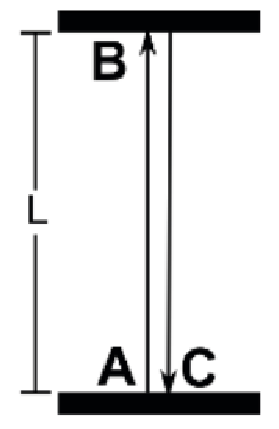
\includegraphics[scale=0.5]{fig2_1.pdf}
    \caption{思想实验图示}
    \label{fig2.1}
}}
设想坐标系中一观察者,在原点处向上发出一个光脉冲,经过一段时间后被垂直镜面反射回原点。如图\ref{fig2.1}所示

有3个重要的事件:
\begin{itemize}
  \item {\bf{A:}}光从原点发出
  \item {\bf{B:}}光在镜面上反射
  \item {\bf{C:}}光回到原点
\end{itemize}
事件{\bf{AC}}之间的时间间隔为\mpar{对于恒定速度$v$而言,有$v=\frac{\Delta s}{\Delta t}$,$\Delta s$表示经过的距离,$\Delta t$代表所需时间,因此$\Delta t=\frac{\Delta s}{v}$}
\begin{equation}\label{equ2.1}
\Delta t=t_C-t_A=\frac{2L}{c}
\end{equation}
式中$L$表示原点与反射点之间的距离。

{\picmpar{
        \centering
        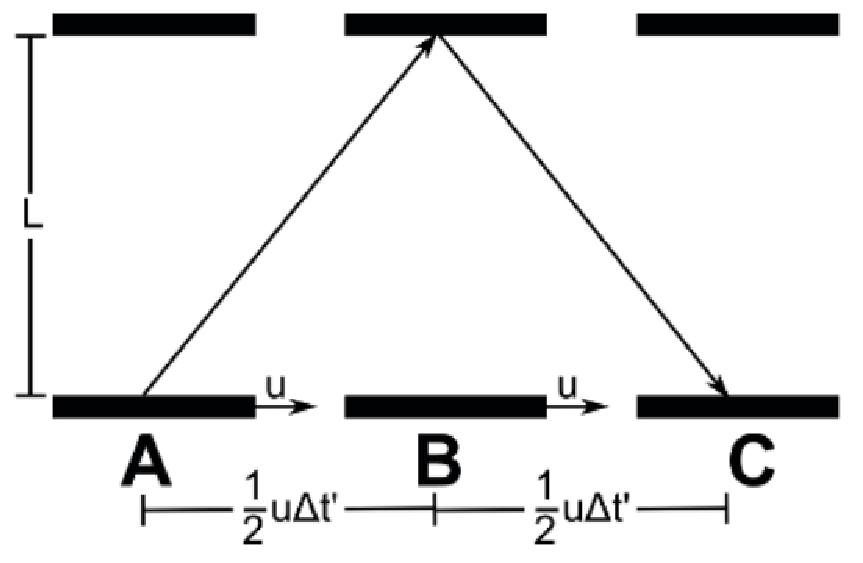
\includegraphics[scale=0.31]{fig2_2.pdf}
        \caption{思想实验图示。 第二位移动观察者向左移动, 因此第一位观察者相对他向右移动}
        \label{fig2.2}
}}


接下来考虑第二位观察者,在$t_A$时刻处于他所在的坐标系的原点,并以恒定速度$u$相对于第一个观察者\mpar{那些能将两相对速度恒定的惯性参考系中的物理量相互转化的变换称为
{\bf{推动(Boost)}}变换, 后面我们会对此进行详述。}向左运动。为简便起见,我们假设第二个参考系的原点在$t_A$时刻与第一位观察者的坐标系原点重合。第二位观察者所见到的现象就与第一位不一样了。在他的参考系中,光脉冲的起点和终点并不在同一位置(见图\ref{fig2.2})。

用数学语言表示:
\begin{equation}\label{equ2.2}
  x'_A=0 \neq x'_C=u \Delta t' \qquad \rightarrow \qquad \Delta x' =u \Delta t'
\end{equation}
带撇物理量代表第二位观察者所测量的量。对于第一位静止系的观察者而言有
\begin{equation}\label{equ2.3}
  x_A=x_C \qquad \rightarrow \qquad \Delta x=0
\end{equation}
假定了第二位观察者运动沿$x$轴,因此
\begin{equation}\label{equ2.4}
 y'_A=y'_C \quad  \quad z'_A=z'_C \quad \rightarrow \quad \Delta y'=0 \quad  \quad \Delta z'=0
\end{equation}
那么同样也有
\begin{equation}\label{equ2.5}
 y_A=y_C \quad  \quad z_A=z_C \quad \rightarrow \quad \Delta y=0 \quad  \quad \Delta z=0
\end{equation}

接下来的问题是:{\bf{第二位观察者所测得的时间间隔是多少?}}因为已经假定了光速为常数,那么事件{\bf{AC}}对于第二位观察者而言将具有不同的间隔!时间间隔$\Delta t'=t'_C-t'_A$,等于光在第二位观察者的参考系中走过的距离$l$除以光速$c$。
\begin{equation}\label{equ2.6}
  \Delta t'=\frac{l}{c}
\end{equation}
我们可以利用古老的Pythagoras\footnote{通译为毕达哥拉斯。}定理(见图\ref{fig2.2}) 计算光传播的距离
\begin{equation}\label{equ2.7}
  l=2 \sqrt{\left(\frac{1}{2} u \Delta t'\right)^2+L^2}
\end{equation}
利用式\eqref{equ2.6}可以得到
\begin{equation}\label{equ2.8}
  c \Delta t' =2 \sqrt{\left(\frac{1}{2} u \Delta t'\right)^2+L^2}
\end{equation}
再利用式\eqref{equ2.2}中的$\Delta x'=u\Delta t'$可得
\begin{displaymath}
c \Delta t' =
  2 \sqrt{\left(\frac{1}{2} u \Delta t'\right)^2+L^2}
\end{displaymath}
\begin{displaymath}
  \rightarrow
  \left( c \Delta t' \right)^2 =
   4 \left( \left(\frac{1}{2} u \Delta t'\right)^2+L^2 \right)
\end{displaymath}
\begin{equation}\label{equ2.9}
\rightarrow
\left( c \Delta t' \right)^2
-\left(\Delta x' \right)^2=
4 \left( \left(\frac{1}{2} u \Delta t'\right)^2+L^2 \right)
-\left(\Delta x' \right)^2 =4L^2
\end{equation}
 现在回到式\eqref{equ2.1},即$\Delta t =\frac{2L}{c}$,那么
\begin{equation}\label{equ2.10}
 \left( c \Delta t' \right)^2
 -\left(\Delta x' \right)^2
 =4 L^2
 =\left( c \Delta t \right)^2
 =\left( c \Delta t \right)^2
 -
 \!\!\!
 \underbrace{\left(\Delta x \right)^2}_{=0 \text{由式}\eqref{equ2.3} \text{知}}
\end{equation}
终于,我们得到\mpar{\it{注意到我们在此处采用的是得到这个结果的最简方法,因为我们假定$t_A$时刻两坐标的原点是重合的。尽管如此,就算我们任意选择两惯性参考系原点的关系,仍然可以证明这个结论,只是过程会复杂一些。因为物理定律在任意惯性系中都是一样的,这给了我们任意选择便于计算的参考系的自由。如果第二位观察者的参考系运动方向是任意的,那就不再有$\Delta y'=0$和$\Delta z'=0$,但虽然如此,我们能够证明方程仍然是成立的,因为物理定律在任意惯性系中都是一样的。$^{\color{red}{4}}$\ \\ \ \\ {$^{\color{red}{4}}$ 译者注:原文的确把这句话说了两遍}}}

\begin{equation}\label{equ2.11}
\left( c \Delta t' \right)^2
-\left(\Delta x' \right)^2
-\underbrace{\left(\Delta y' \right)^2}_{=0}
-\underbrace{\left(\Delta z' \right)^2}_{=0}
=
\left( c \Delta t \right)^2
-\underbrace{\left(\Delta x \right)^2}_{=0}
-\underbrace{\left(\Delta y \right)^2}_{=0}
-\underbrace{\left(\Delta z \right)^2}_{=0}
\end{equation}
考虑第三个观察者,相对于第一个观察者以不同的速度运动,用同样的推理可以得到
\begin{equation}\label{equ2.12}
\left( c \Delta t'' \right)^2
-\left(\Delta x'' \right)^2
-\left(\Delta y'' \right)^2
-\left(\Delta z'' \right)^2
=
\left( c \Delta t \right)^2
-\left(\Delta x \right)^2
-\left(\Delta y \right)^2
-\left(\Delta z \right)^2
\end{equation}
因此,我们得到了一些对于所有观察者都相同的量:即二次型
\begin{equation}\label{equ2.13}
(\Delta s)^2
\equiv\left( c \Delta t \right)^2
-\left(\Delta x \right)^2
-\left(\Delta y \right)^2
-\left(\Delta z \right)^2
\end{equation}

此外,我们还能看出对于不同观察者,$(\Delta x)^2+(\Delta y)^2+(\Delta z)^2$或者说$(c\Delta t)^2$是不同的。我们将在下一节讨论不变量$\Delta s^2$所蕴含的物理意义。


\section[固有时]{Proper Time \quad 固有时}
\label{sec2.2}
我们在上一节推导出了狭义相对论中的不变量$\Delta s^2$,其在所有观察者眼中都相同。接下来我们要讨论这个量的物理意义。
    \picmpar{
        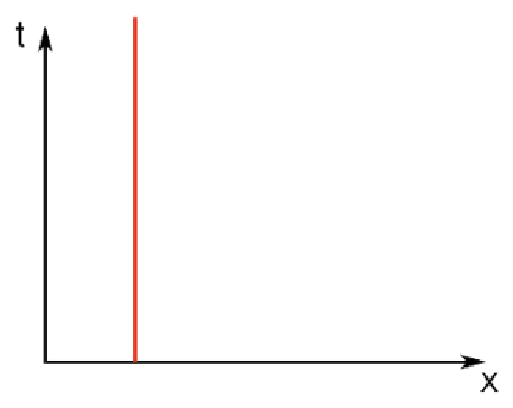
\includegraphics[scale=0.4]{fig2_3.pdf}
        \caption{静止物体的世界线。物体位置不随时间流逝而变化。}\label{fig2.3}
    }
为简便起见,我们将问题限制在一维空间中。对于一个相对于观察者静止的物体,我们能作出它的时空图(见图\ref{fig2.3})。相应的,一个匀速运动的物体能作出如图\ref{fig2.4}所示的时空图。

    \picmpar{
        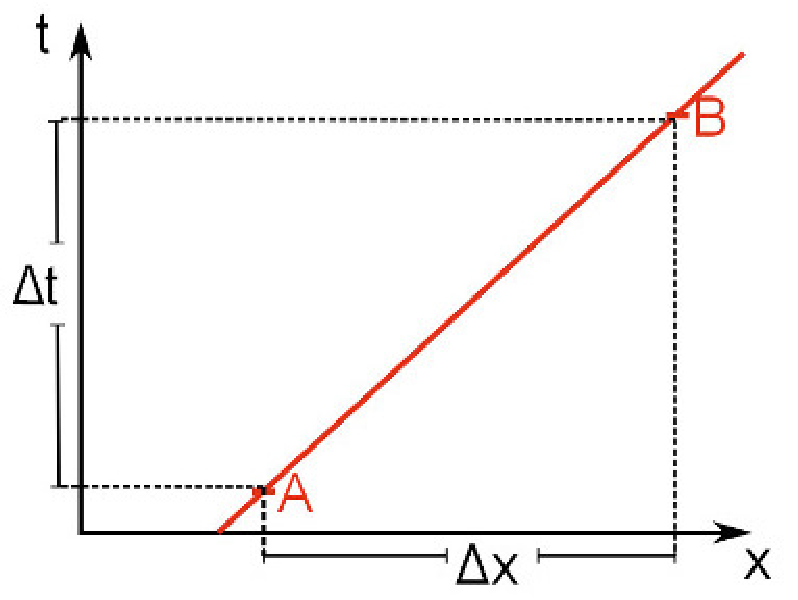
\includegraphics[scale=0.35]{fig2_4.pdf}
        \caption{某匀速直线运动物体的世界线。物体前后经过某两点记为事件A,B。它们间的空间距离为$\Delta x$,时间间隔为$\Delta t$}\label{fig2.4}
    }
我们画来用于确定物体在时空中位置的线称为{\bf{世界线(world line)}}。世界线总是依赖于观察者的。两不同观察者对于同一物体可能会画出完全不同的世界线。若一观察者眼中的物体时空图为图\ref{fig2.4},那么对于速度与物体相同的观察者,其时空图将为图\ref{fig2.5},即对于此观察者物体静止。为了解释两位观察者给出的不同描述,我们引入$x'$ 和$t'$ 表示第二位观察者的参考系中的时间和位置。\footnote{注意:我们这里使用的例子与节\ref{sec2.1}不同}

我们可以看到,两个观察者将对事件$AB$之间的变化持不同观点。对于第一位观察者,$\Delta x \neq 0$, 但对于第二位观察者,$\Delta x' = 0$。 两观察者都认为事件$A$ 和$B$ 之间的时间间隔非零:$\Delta t \neq 0$ 和$\Delta t' \neq 0$,且认为$\Delta s^2$也相同(见上节推导的结论,任意观察者都有相同的$\Delta s^2$)。 这将导出一个令人惊讶的结论:事件$A$ 到$B$ 经历的时间对于两观察者不同
    \picmpar{
        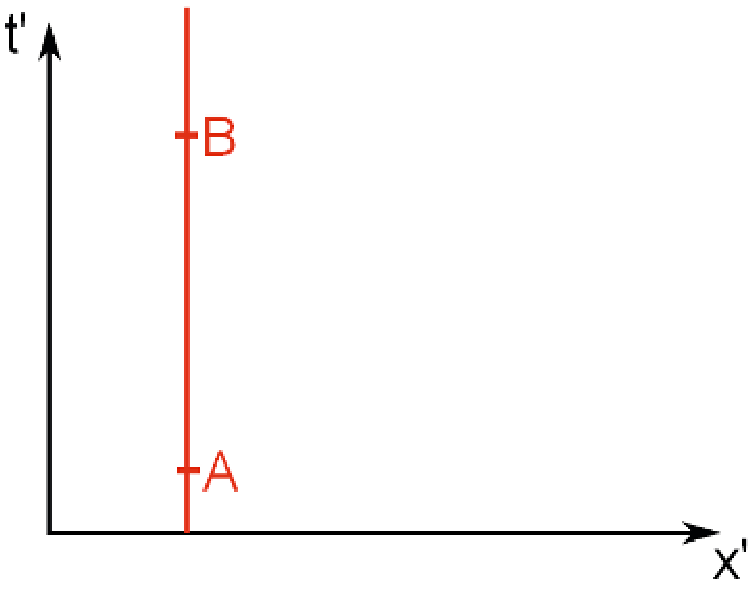
\includegraphics[scale=0.35]{fig2_5.pdf}
        \caption{同一个运动物体的世界线,但观察者与该物体速度相同。该观察者观测到的事件AB之间的空间距离为$\Delta x' = 0$}\label{fig2.5}
    }
\begin{equation}\label{equ2.14}
  (\Delta s)^2
  =(c\Delta t)^2
  -(\Delta x)^2
\end{equation}
\begin{equation}\label{equ2.15}
  (\Delta s')^2
  =(c\Delta t')^2
  -\underbrace{(\Delta x')^2}_{=0}
  =(c\Delta t')^2
\end{equation}
\begin{equation}\label{equ2.16}
   (\Delta s)^2
   = (\Delta s')^2
   \rightarrow
    (\Delta t')^2 \neq
     (\Delta t')^2
     \quad \text{因为}  (\Delta x)^2 \neq 0
\end{equation}

这是有关狭义相对论最著名的一个效应,通常称为{\bf{钟慢效应(time-dilation)}}。时间间隔依赖于观察者,正如空间距离一样。不同观察者时间流逝速度不同,因此两事件经历的时间也就自然不同了。

现在时间将变为一个相对的概念,如果我们能找到一个对于所有观察者都相同的时间量,这将会非常有用。在上述例子中,第二位观察者与物体有相同的速度,有
\begin{equation}\label{equ2.17}
  (\Delta s')^2
  =(c\Delta t')^2
\end{equation}

上式意味着狭义相对论中的不变量恰为观察者所观测到的时间间隔乘上光速$c$。这让我们有机会能用$(\Delta s)^2$定义一个对于所有观察者相同的时间量。我们定义
\begin{equation}\label{equ2.18}
  (\Delta s)^2
  =(c\Delta \tau)^2
\end{equation}
$\tau$称为{\bf{固有时(proper time)}}。固有时是所有相对于该物体静止的观察者所测量的时间。

当然,现实生活中的物体绝非只能做匀速运动,但我们可以取足够短的时间(无穷小),使得运动近似为匀速运动,这样固有时的概念就说得通了。因此数学上我们需将概念过渡到无穷小,即$\Delta \rightarrow d$:
\begin{equation}\label{equ2.19}
  (ds)^2  =(cd \tau )^2=(cdt)^2-(dx)^2-(dy)^2-(dz)^2
\end{equation}

因此,就算一个物体到处乱跑,我们也能假设一个与物体一起运动的自带时钟的观察者,这样他总与该物体相对静止。对于这个特定的观察者而言,他所测量的时间间隔就是固有时,这一数值对其余观察者也是相同的,因为$(ds)^2=(cd\tau)^2$对于任意观察者成立。再次强调,这并不意味着对所有观察者都有同样的时间间隔,只是这些观察者承认该特殊观察者所测量的时间间隔为一不变量罢了。

\section[速度上限]{Upper Speed Limit \quad 速度上限}
\label{sec2.3}
在上节中我们对狭义相对论这一不变量有了解释,现在可以更进一步,导出另一个狭义相对论的惊人结论。

由于不变量的定义中带有负号,这意味着对于时空中的两个事件,$(\Delta s)^2$的值可能为0。$(\Delta s)^2$的值甚至可能是负的,但这样我们将得到一个复的固有时\mpar{按固有时定义,$(ds)^2=(cd\tau)^2$,$(ds)^2 < 0 \rightarrow d\tau$ 为复数。},通常复的固有时没有物理意义。因此,$(\Delta s)^2=0$时固有时最小,$\tau=0$,令
\[
\Delta s^2_{min}
=0=(c \Delta t)^2-(\Delta x)^2-(\Delta y)^2-(\Delta z)^2
\]
\[
\rightarrow (c \Delta t)^2
=(\Delta x)^2+(\Delta y)^2+(\Delta z)^2
\]
\begin{equation}\label{equ2.20}
 \rightarrow c^2=
  \frac{(\Delta x)^2+(\Delta y)^2+(\Delta z)^2}{(\Delta t)^2}
\end{equation}
在上式右侧我们有速度平方$v^2$,也就是距离除上时间,把这个式子写成极限,则
\begin{equation}\label{equ2.21}
 \rightarrow c^2=\frac{(d x)^2+(d y)^2+(d z)^2}{(dt)^2}
\end{equation}
函数$x(t)$,$y(t)$,$z(t)$是描述两事件之间路径的参数方程,这样式子右侧就是两事件间的运动速率。
%flag 此处的速度在文中并无主语,可能要加上物体二字,那么前面也得改。

因此,当某一观察者测得的固有时为$0$时其速度将满足下式
\begin{equation}\label{equ2.22}
  \rightarrow c^2 =v^2
\end{equation}
这意味着没有物体能以超过光速$c$的速度运动!\footnote{译者注:否则其固有时为复}{\bf{我们给物理学中的一切事物找到了一个速度上限。}}时空中的两事件相互影响的传播速度不能超光速。

{\it{这一点满足物理学上的{\bf{局域性原理(principle of locality)}},即物理学中的对象只能被它邻近的对象影响。相互作用都是局域的,不存在超距作用,物理效应的传播需要时间。}}

\section[Minkowski记法]{The Minkowski Notation \quad Minkowski 记法}
\label{sec2.4}
\begin{quote}
从现在起,孤立的空间和孤立的时间注定要消失成为影子,只有两者的统一才能保持独立的存在。
\end{quote}
\begin{flushright}
  {\bf{-Hermann Minkowski}}\mpar{出自Hermann Minkowski在Assembly of German Natural Scientists and Physicians(1908.9.21)上的演讲}
\end{flushright}
写出狭义相对论中不变量
\begin{equation}\label{equ2.23}
 ds^2=(cdt)^2-(dx)^2-(dy)^2-(dz)^2
\end{equation}
在此处将采用一种新的记法,这种记法初学时可能稍显复杂,不过后文中将经常用到:\\
\begin{align}
ds^2&=\eta^{\mu\nu}dx_\mu dx_\nu \notag \\
&=\eta^{00}(dx_0)^2+\eta^{11}(dx_1)^2+\eta^{22}(dx_2)^2+\eta^{33}(dx_3)^2 \notag \\
&=dx_0^2-dx_1^2-dx_2^2-dx_3^2\notag \\
&=(cdt)^2-(dx)^2-(dy)^2-(dz)^2 \label{equ2.24}
\end{align}
在这里我们用了一些新的约定和记号,这些东西在近代物理中应用很广泛,所以越早熟悉越好:
\begin{itemize}
  \item Einstein求和约定:某指标在同一项内出现两次则代表遍历该指标并求和。例如:$\sum_{i=1}^3a_i b_i =a_i b_i=a_1 b_1 +a_2 b_2 +a_3 b_3$,但$\sum_{i=1}^3a_i b_j=a_1 b_j +a_2 b_j +a_3 b_j\neq a_i b_j$
  \item 像$\mu$,$\nu$,$\sigma$这样的希腊字母
  \mpar{像 $i$,$j$,$k$这样的罗马字母作指标时一般代表从1到3求和:$x_i x_i \equiv \sum_i^3 x_i x_i$。 后面我们还会用到大写的罗马字母如$A$,$B$,$C$,它们作指标时代表从1到8求和。} 作指标时,一般代表从0 到3 求和:$x_\mu y_\mu=\sum_{\mu=0}^3 x_\mu y_\mu $
  \item 我们约定变量$x_0\equiv ct$,$x_1\equiv x$,$x_2\equiv y$,$x_3\equiv z$。这样时间空间地位等同,也便于我们使用Einstein求和约定
  \item 引入Minkowski度规($\eta$看作一矩阵,$\eta^{ij}$ 为其矩阵元):$\eta^{00}=1$,$\eta^{11}=-1$,$\eta^{22}=-1$,$\eta^{33}=-1$,当$\mu \neq \nu$时$\eta^{\mu\nu}=0$  (也可以等价的写为
\mpar{$\eta^{\mu\nu}= \\ \\
       \left(
       \begin{array}{cccc}
        1 & 0 & 0 & 0 \\
         0 & -1 & 0 & 0 \\
          0 & 0 & -1 & 0 \\
          0 & 0 & 0  & -1\\
        \end{array}
        \right)$ }
      $\eta^{\mu\nu} = \mathrm{diag} (1,-1,-1,-1)$)
\end{itemize}

另外按常规我们还要引入{\bf{四维矢量(four-vector)}},简称{\bf{4矢}}。
\begin{equation}\label{equ2.25}
  dx_\mu =\left(\begin{array}{c}
            dx_0 \\
            dx_1 \\
            dx_2 \\
            dx_3
          \end{array}\right)
\end{equation}
式\eqref{equ2.24}可用4矢和Minkowski度规表出
\begin{align}
  &(ds)^2=dx_\mu \eta^{\mu\nu} dx_\nu \notag \\
  &=\left(
     \begin{array}{cccc}
       dx_0 & dx_1 & dx_2 & dx_3 \\
     \end{array}
   \right)
   \!\!\!
   \left(
     \begin{array}{cccc}
       1 & 0 & 0 & 0 \\
       0 & -1 & 0 & 0 \\
        0 & 0 & -1 & 0 \\
        0 & 0 & 0  & -1\\
     \end{array}
   \right)
   \!\!\!
   \left(
     \begin{array}{c}
       dx_0 \\
        dx_1 \\
       dx_2 \\
        dx_3\\
     \end{array}
   \right)\notag \\
   &=dx_0^2-dx_1^2-dx_2^2-dx_3^2 \label{equ2.26}
\end{align}

采用这种记法能让我们省不少事。对于$ds$,我们给出的解释是时空(Minkowski时空)中两事件的“距离”,这个“距离”并不只是空间距离,它还将时间间隔考虑在内。如果我们考虑3维Euclidean 空间\mpar{3维Euclidean空间就是经典物理中一般的空间,在此空间中我们将时间和空间分别处理,也就是未将时空考虑成一个整体的几何结构来考虑。但一旦将时间作为新坐标,结合出时空的观念,我们便能将时间空间放在同一坐标下考虑。}中两点间最短距离的平方\mpar{Kronecker函数$\delta_{ij}$即是单位矩阵在指标记法下的表示,详见附录\ref{appendix.B.5.5}}
\begin{align}
  (ds)^2&=dx_i \delta^{ij} dx_j \notag \\
            &=\left(
               \begin{array}{ccc}
                dx_1 & dx_2 & dx_3 \\
               \end{array}
               \right)
               \left(
               \begin{array}{ccc}
                1 & 0 & 0  \\
                0 & 1 & 0  \\
                0 & 0 & 1  \\
              \end{array}
              \right)
              \left(
              \begin{array}{c}
               dx_1 \\
               dx_2 \\
               dx_3\\
              \end{array}
              \right)\notag \\
           &=(ds)^2=(dx_1)^2+(dx_2)^2+(dx_3)^2\label{equ2.27}
\end{align}

这种数学工具叫{\bf{度规(metric)}},它能够告诉我们无限临近的两点之间的距离。在Euclidean空间中度规就是单位矩阵$\delta_{ij}$。在广义相对论的弯曲时空中将会有更复杂的度规,但在狭义相对论中我们采用的是相对简单的Minkowski度规$\eta^{\mu\nu}$。度规是计算长度的工具,我们可以通过度规定义{\bf{4矢的长度(length of a four-vector)}},即4矢与自身的标量积\mpar{此定义在Euclidean空间中同样适用:由于度规为
$\delta_{ij}=\left(
 \begin{array}{ccc}
 1 & 0 & 0  \\
  0 & 1 & 0  \\
  0 & 0 & 1  \\
  \end{array}
  \right)
$,易得矢量$\vec{v}$的长度$=\vec{v}\cdot\vec{v}=v_1^2+v_2^2+v_3^2$。}
\[
x^2=x \cdot x \equiv x_\mu x_\nu \eta^{\mu\nu}
\]
类似地,两任意4矢的标量积定义为
\begin{equation}\label{equ2.28}
  x\cdot y\equiv x_\mu y_\nu \eta^{\mu\nu}
\end{equation}

对于上下标,也有一些约定能使计算过程更清晰。我们定义带有 上指标的4矢\mpar{带有下指标的4矢通常叫做协变4矢,带有上指标的4 矢通常叫做逆变4矢。}
\begin{equation}\label{equ2.29}
  x^{\mu}\equiv\eta^{\mu\nu}x_\nu
\end{equation}
或者
\begin{equation}\label{equ2.30}
  y^{\nu}\equiv\eta^{\mu\nu}y_\mu
 \!\!\!\!\!\!\!\!\!\!\!\!\!\!\!\!\!\!\!\!\!\!\!\!\!\!\!\!
 \underbrace{=}_{Minkowski\text{度规是对称的}\eta^{\mu\nu}=\eta^{\nu\mu}}
 \!\!\!\!\!\!\!\!\!\!\!\!\!\!\!\!\!\!\!\!\!\!\!\!\!\!\!\!
  \eta^{\nu\mu}y_\mu
\end{equation}
因此,标量积可以写为\mpar{指标的名称如何选取并不影响最后的值,详见附录\ref{appendix.B.5.1}。}
\begin{equation}\label{equ2.31}
  x\cdot y\equiv x_\mu y_\nu \eta^{\mu\nu}=x_\mu y^\mu=x^\nu y_\nu
\end{equation}
上式中,变换的上指标是可以任意选择的,这只是为了避免公式中总是出现$\eta^{\mu\nu}$的一种方法,正如引入Einstein求和约定是为了避免总是出现求和号一样。

\section[Lorentz变换]{Lorentz Transformations \quad Lorentz变换}
\label{sec2.5}
下一步,我们将尝试找出两参考系之间不违背狭义相对论基本假设的变换方式。由上文可知,从狭义相对论的两个基本假设可以推出对于所有惯性参考系均有$ds^2=\eta^{\mu\nu} dx_\mu dx_\nu $,即
\begin{equation}\label{equ2.32}
  ds'^2= dx'_\mu dx'_\nu \eta^{\mu\nu}
  =ds^2
  =dx_\mu dx_\nu\eta^{\mu\nu}
\end{equation}
因此,两参考系间所允许的变换要能保证这个二次式的形式,和Minkowski时空中的标量积在变换下不变。设变换为$\Lambda$,那么变换后
\begin{equation}\label{equ2.33}
  dx_\mu \rightarrow dx'_\mu=\Lambda^\sigma_\mu dx_\sigma
\end{equation}
由于$(ds)^2$在变换下不变
\begin{align}
(ds)^2&=(ds')^2 \notag\\
\rightarrow dx\cdot dx &\overset{\text{!}}{=} dx' \cdot dx' \notag \\
\rightarrow dx_\mu dx_\nu\eta^{\mu\nu} &\overset{\text{!}}{=} dx'_\mu dx'_\nu\eta^{\mu\nu} \underbrace{=}_{\mathclap{\eqref{equ2.33}\text{式}}} \Lambda_\mu^\sigma dx_\sigma \Lambda_\nu^\gamma dx_\gamma\eta^{\mu\nu}\notag \\
\underbrace{\rightarrow}_{\mathclap{\text{重命名哑指标}}} dx_\mu dx_\nu\eta^{\mu\nu} &\overset{\text{!}}{=} \Lambda^\mu_\sigma dx_\mu \Lambda^\nu_\gamma dx_\nu\eta^{\sigma\gamma}\notag\\
\underbrace{\rightarrow}_{\mathclap{因为dx_\nu\text{任意}}} \eta^{\mu\nu} &\overset{\text{!}}{=} \Lambda^\mu_\sigma\Lambda^\nu_\gamma\eta^{\sigma\gamma}\label{equ2.34}
\end{align}
或者用矩阵形式来写\mpar{详见附录\ref{appendix.C.1}。}
\begin{equation}\label{equ2.35}
  \eta=\Lambda^{\mathrm{T}}\eta\Lambda
\end{equation}

{\bf{此即变换$\Lambda_\mu^\nu$所需满足条件。}}

这个条件现在看起来可能有些奇怪,但在后文中我们会用更自然的方式导出这个条件。在下一章里,我们会看到Euclidean空间中的旋转所导出的变换%
\mpar{稍后会讲明$O$的意义。}$O$能够保证Euclidean 空间的标量积不变\mpar{“$\cdot$”表示的是矢量的点乘,如果我们将矢量写为列向量,那么按矩阵相乘的定义有$\vec{a}\cdot\vec{b}=\vec{a}^\mathrm{T}\cdot\vec{b}$。 有关$(Oa)^\mathrm{T}=a^\mathrm{T}O^\mathrm{T}$这一点详见附录\ref{appendix.C.1},式\ref{equC.3}。}% 此处原文有误
\begin{equation}\label{equ2.36}
  \vec{a} \cdot \vec{b}
  \overset{\text{!}}{=}
  \vec{a'} \cdot \vec{b'}
  \underbrace{=}_{\mathclap{\text{注意} (Oa)^\mathrm{T}=a^\mathrm{T}O^\mathrm{T}}}
  \vec{a}^\mathrm{T} O^\mathrm{T} O\vec{b}
\end{equation}
因此
\mpar{这一条件一般称为{\bf{正交性(orthogonality)}}条件,因此用字母$O$表示。满足$O^\mathrm{T} O={\bf{1}}$的矩阵称为正交矩阵,因为它列与列之间是正交的。换句话说,矩阵的每一列都可以看做一个矢量,正交性条件就是说这些矢量相互正交。}

$O^\mathrm{T} {\bf{1}} O\overset{\text{!}}{=}{\bf{1}}$,恰巧Euclidean 空间的度规就是单位矩阵${\bf{1}}$,其地位正如Minkowski 度规在式\eqref{equ2.35} 中一样。这个性质是旋转的定义中的一部分,旋转不能改变矢量的长度,即在数学上保证标量积不变
\mpar{矢量的长度即是矢量与自身的标量积的平方根。}$^{,}$\footnote{译者注:$\vec{a}\cdot \vec{b}=\frac{1}{2} [(\vec{a}+\vec{b})^2-\vec{a}^2-\vec{b}^2]$,若保证模长不变,标量积也不变。}此外我们还注意到旋转不改变坐标系的手向\mpar{详见附录\ref{appendix.A.5}。},这表明 $\text{det}(O) \overset{\text{!}}{=}1$,因为保证标量积不变的变换除了旋转变换还有空间反演\mpar{空间反演可简单地理解为映射$\vec{x}\rightarrow -\vec{x}$。这种变换满足$\text{det}(O) \overset{\text{!}}{=}$及$O^{\mathrm{T}}O={\bf{1}}$。 因此,如果我们要将变换限制为旋转变换,就需要加上条件$\text{det} (O) \overset{\text{!}}{=} {\bf{1}}$。此外,空间反演变换又称宇称变换。}。

我们定义保Minkowski时空中标量积不变的变换为
{\bf{Lorentz变换(Lorentz transformations)}}
,这也是为保证狭义相对论的假设所必需的。相应的,每当我们需要得到在Lorentz变换下不变的项时,{\it{都必须结合上下指标}}:$x_\mu y^\mu=x_\mu y_\nu \eta^{\mu\nu}$。
在学会一些非常优雅的技术来处理这样的情况之后,我们会在下一章构建这些转换具体的矩阵形式。


\section[不变性,对称性,协变性]{Invariance, Symmetry and Covariance 不变性,对称性,协变性}
在继续之前,我们有一些重要的概念要事先声明。首先,一个量能被称为{\bf{不变量(invariant)}},这个量必须在变换下不变。比如说,我们考虑一个依赖于不同参数$A,B,C,\dots$的任意函数$ F$,$F=F(A,B,C,\dots)$,如果我们将$A,B,C,\dots$变换为$A',B',C',\dots$,有
\begin{equation}\label{equ2.37}
  F(A',B',C',\dots)=F(A,B,C,\dots)
\end{equation}
那么$F$称为变换下的一个不变量。我们可以用对称性来描述。
{\bf{对称性(symmetry)}}是指在某一变换下或者某一系列变换下保持不变的性质。举个例子,如果说一个物理系统在任意的旋转变换下不变,那么该系统具有旋转对称性。再比如说,一间室温为常温的房间,房间内各点的温度与位置无关,换言之,如果把所有的点朝着某特定方向平移一段距离,室温不变。因此我们说室温具有{\it{平移对称性}}。

协变性与不变性有共通之处而又不同。如果一个方程在变换下形式不变,那么称这个方程具有协变性。例如下面这个式子
\[
E_1=a A^2+bBA'+cC^4
\]
在变换之后这个方程写为
\[
E'_1=a A'^2+bB'A'+cC'^4
\]
那么这个方程具有协变性,因其在变换下形式不变。另一方程
\[
E_2=x^2+4axy+z
\]
若在变换之后写为
\[
E'_2=y'^3+4az'y'+y'^2+8z'x'
\]
那么它就不是协变的,因为其形式已经变化。

所有的物理规律都应具有Lorentz协变性\footnote{即在Lorentz变换下具有协变性——译者(InSight)},因为只有这样的物理规律才能在任意参考系下成立。非协变的物理规律只能在某一特定参考系下成立,这会导致在东京和纽约具有不同的物理规律。显然这个主意糟透了,因为不应该存在一个特殊的参考系,我们得让物理规律在任意参考系中成立。后面我们将讲述如何用协变的方法来计算物理规律。

\section*{Further Reading Tips\quad 阅读建议}
\begin{itemize}
\item {\bfseries E.Taylor and J.Wheeler - Spacetime Physics:Introduction to Special Relativity}\mpar{Edwin F.Taylor and John Archibald Wheeler.\\ {\itshape Spacetime Physics}.\\W.H.Freeman,2nd edition,\\3 1992.ISBN 9780716723271}适合用来入门。
\item {\bfseries D.Fleisch - A Student's Guide to Vectors and Tensors}\mpar{Daniel Fleisch.\\{\itshape A Student's Guide \\ to Vectors and Tensors}.\\ Cambridge
University Press,\\1st edition,11 2011.ISBN 9780521171908}对狭义相对论中用到的张量范式有很有创意的解释。比如对于协变与逆变分量的差异。
\item {\bfseries N.Jeevanjee - An Introduction to Tensors and Group Theory for Physicists}\mpar{Nadir Jeevanjee. \\{\itshape An Introduction to Tensors and Group Theory for Physicists}.\\Birkhaeuser,1st edition,August 2011.\\ISBN 978-0817647148}是另一本把在狭义相对论中用到的数学讲的不错的书。
\item {\bfseries A.Zee - Einstein Gravity in a nutshell}\mpar{Anthony Zee.\\{\itshape Einstein Gravity in a
Nutshell}.\\Princeton University Press,\\1st
edition,5 2013.\\ISBN 9780691145587}是一本关于广义相对论的书,但是里面也有很多关于狭义相对论的很棒的解释。
\end{itemize}

%!TEX encoding = UTF-8 Unicode

\part{Symmetry Tools 对称性工具}

\begin{partquote}
{\bfseries “数字是大小的度量,群是对称性的度量。”}\marginpar{``Numbers measure size, groups measure symmetry.''}


\begin{flushright}
--- Mark A.Armstrong\\
in {\itshape Groups and Symmetry.}
\marginpar{%
Groups and Symmetry.\\
Springer,2nd edition,2 1997.
ISBN 9780387966755
}
\end{flushright}
\end{partquote}


%!TEX root = ./../main.tex
%!TEX encoding = UTF-8 Unicode
%----------------------------------------------------------------------------------------
%	CHAPTER 3
%	Translator: SI(= Surgam Identidem), InSight
%	Proofreader: lh1962, laserdog
%----------------------------------------------------------------------------------------

\chapterimage{chapter_head_1.pdf} % Chapter heading image

\begin{quote}
{\bfseries “数字是大小的度量,群是对称性的度量。”}\marginpar{``Numbers measure size, groups measure symmetry.''}


\begin{flushright}
--- Mark A.Armstrong\\
in {\itshape Groups and Symmetry.}
\marginpar{%
Groups and Symmetry.\\
Springer,2nd edition,2 1997.
ISBN 9780387966755
}
\end{flushright}
\end{quote}

\chapter[Lie群]{Lie Group Theory\quad  Lie群}
\label{chap3}

\section*{本章概述}



\marginpar{


下面的图表是本章结构的示意图。 当你迷失方向的时候记得回来看看, 初学的时候不太需要看它。

\setlength{\unitlength}{0.8cm}
\begin{picture}(4, 3)\thicklines
\put(1.5, 1.8){\makebox(2.5, 1.2){\text{二维旋转}}}
\put(1, 0.7){\vector(1, 1){1.4}}
\put(4, 0.7){\vector(-1, 1){1.4}}
\put(0.5, 0.2){\makebox{$\mathcal{U}(1)$}}
\put(4, 0.2){\makebox{$\mathcal{SO}(2)$}}
\put(0, 0){\line(5, 0){5.5}}
\end{picture}

\begin{picture}(4, 3)\thicklines
\put(1.5, 1.8){\makebox(2.5, 1.2){\text{三维旋转}}}
\put(1, 0.7){\vector(1, 1){1.4}}
\put(4, 0.7){\vector(-1, 1){1.4}}
\put(0.5, 0.2){\makebox{$\mathcal{SU}(2)$}}
\put(4, 0.2){\makebox{$\mathcal{SO}(3)$}}
\put(0, 0){\line(5, 0){5.5}}
\end{picture}

\begin{picture}(5, 5)\thicklines
\put(1.5, 4){\makebox(2.5, 1.2){\text{Lorentz变换}}}
\put(2.5, 4.3){\vector(0, -1){0.8}}
\put(1.5, 2.5){\makebox(2.5, 1.2){ \text{Lie代数} $\hat{=} \, \mathfrak{su}(2) \oplus \mathfrak{su}(2) $  }}
\put(2.5, 2.8){\vector(0, -1){0.8}}
\put(1.5, 1){\makebox(2.5, 1.2){\text{双覆盖表示}}}
\put(0, 1){\line(5, 0){5.5}}
\end{picture}

\begin{picture}(5, 3)\thicklines
\put(1.5, 3){\makebox(2.5, 1.2){\text{Lorentz变换 + 平移}}}
\put(2.5, 3.2){\vector(0, -1){0.8}}
\put(1.5, 1.6){\makebox(2.5, 1.2){ \text{Poincar\'e群} }}
\end{picture}

}

本章的最终目的是导出{\bf{Poincar\'e群双覆盖的基本表示}}, 物理学现在认为Poincar\'e群是时空根本的对称性群。 这些基本表示是描述所有基本粒子的必要工具, 每一种表示对应一种基本粒子, 它们揭示了自然界存在何种基本粒子。

我们从两个简单例子引出{\bf{群}}的定义, 然后作为学习Lie群理论的第一步, 我们讨论描述二维旋转变换的两种方式:
\begin{itemize}
	\item $2 \times 2$旋转矩阵。
	\item 单位复数\footnote{指模长为$1$的复数。}。
\end{itemize}
%\mathcal 会覆盖 \bf,这里的SU(2)与原书一样改用黑体
接着我们尝试找出描述三维旋转的第二种方法(像复数那样, 当然第一种方法是$3\times3$矩阵), 第二种方法法与一种超级重要的群——{\bf{$SU(2)$}}\mpar{$S$表示特殊(special), 它的含义为$\det (M) = 1$。 U表示幺正: $M^\dagger M = 1$, 数字$2$表示这个群起初是用$2 \times 2$矩阵定义的。}有关。 之后我们研究{\bf{Lie代数}}, 使用相对简单的Lie代数就能深入研究复杂的Lie群。 不同的群可以有相同的Lie代数, 但只有其中的一部分是基本的。
从上述基础出发就能准确揭示自然的基本对称性群——Poincar\'e群的双覆盖。
%flag1:  double covers the Poincar\'e group。 (Poincar\'e 群的双覆盖) 翻译是否正确?
%ZRQ:感觉可以
我们将利用已知的变换操作导出Lie代数, 并利用Lie代数得出对称变换的不同表示。 这样就能看出开始时使用的表示其实只是一种特殊情况。 于是又能研究Poincar\'e群的重要部分——{\bf{Lorentz群}}, 我们会看到Lorentz群双覆盖的Lie代数由两份$\mathfrak{su}(2)$\, Lie代数所组成, 因此可以直接利用我们熟悉的$\mathcal{SU}(2)$群的结论。 最后将平移变换考虑进来, 就得到了Poincar\'e群, Poincar\'e群就是Lorentz群加上平移。 完成上述所有之后我们终于可以将Poincar\'e群双覆盖的基本表示进行分类, 这些在后面的章节中会大用特用, 我们将从中导出物理学的基本定律。

\section[群]{Groups\quad 群}
\label{sec3.1}
我们需要合适的数学工具描述对称性。 描述对称的数学分支称为{\bf{群论}},而其中物理中经常遇到的连续对称性则需要群论的一个分支{\bf{Lie理论}}来进行描述。

我们把对称性定义为变换下的不变性, 而描述对称的群就定义为某些变换的集合。 让我们从两个简单例子开始体会群到底该怎么定义:



\begin{enumerate}
	\item 正方形在数学上是一些点的集合(例如四个顶点是该集合的一部分),正方形的对称性是指在某些变换下(变换: 将一个点映射到另一个点)保持不变(点集自身被映射回自身)的性质。\footnote{译者注:原文里把对称性定义为了一种\underline{变换},而不是在某种变换下不变的\underline{性质}(a symmetry of the square is a \underline{transformation} that maps this set of points into itself.),但是后面又说`Symmetry means \underline{invariance under a transformation}',这里翻译时有些改变。另外后文中不少也是意译,不妨参考原文阅读。(QZR)}

	符合条件的变换有绕中心旋转$90^\circ, 180^\circ, 270^\circ, 0^\circ$等等。 这些旋转操作将正方形映射到它自身。这意味着把集合里的每个点都映射回了集合里。我们称这个集合(正方形点集)在这样的变换下具有不变性。
	% flag1: This means they map every point of the set to a point that lies again in the set 没翻译, 因为觉得太啰嗦...
	%我还是补上了,请管理员考虑是否merge

	\picmpar{
		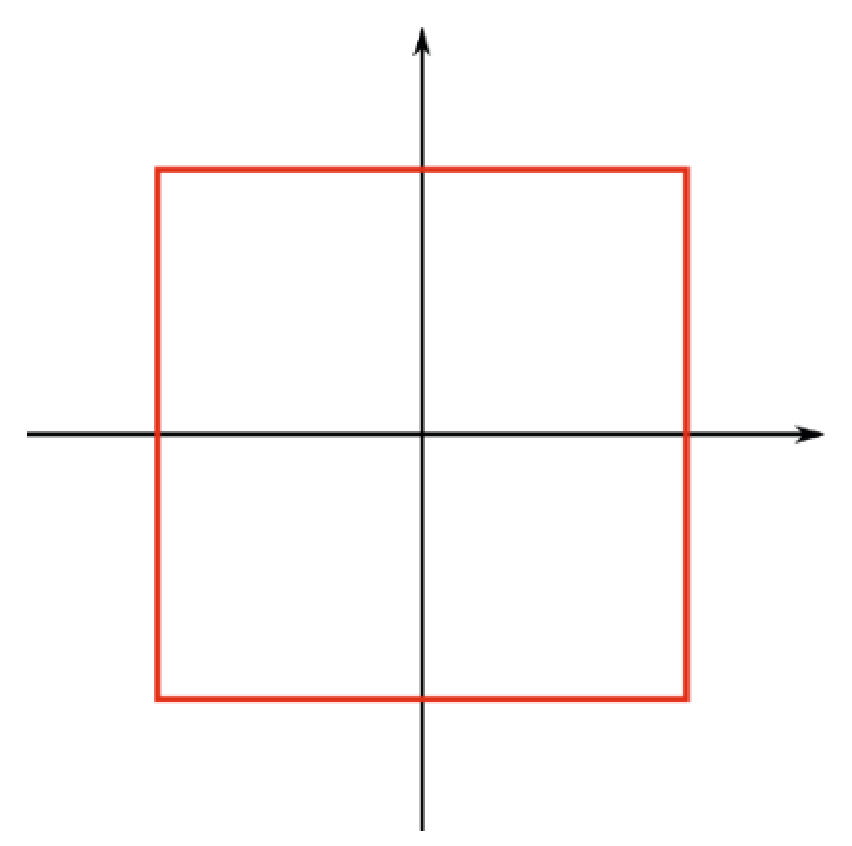
\includegraphics[scale=0.35]{fig3_1}
		\caption{正方形}
	}

	\picmpar{
		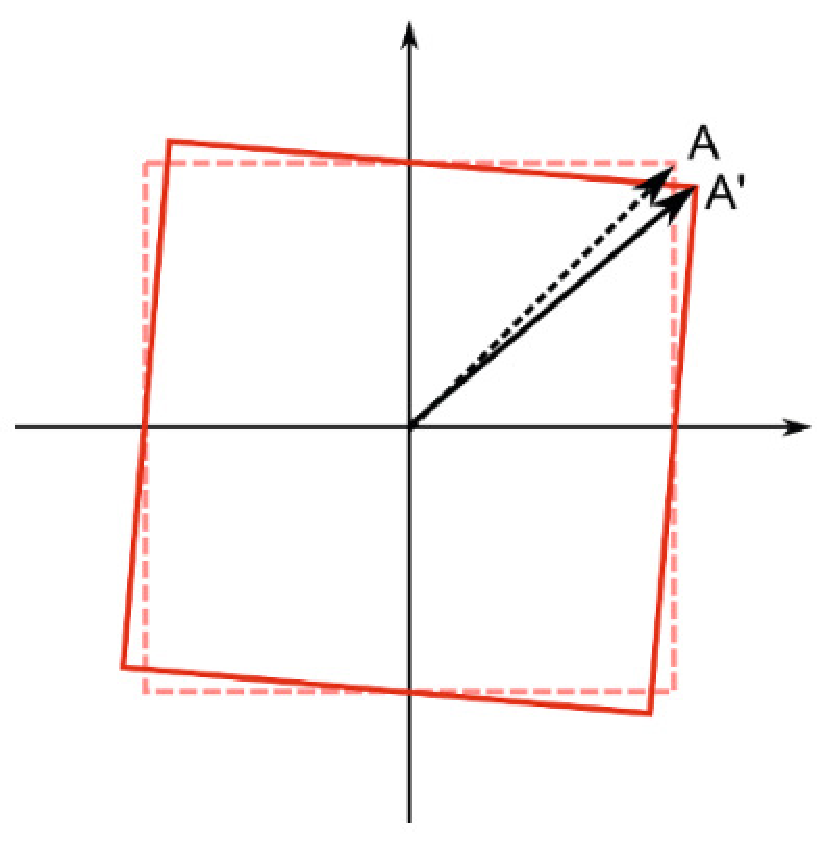
\includegraphics[scale=0.35]{fig3_2.pdf}
		\caption{正方形绕中心顺时针旋转$5^\circ$}
	}

	注意不是所有旋转变换对于正方形都是对称的。 如果我们关注顶点的变化就容易看出来, 比如绕中心顺时针旋转$5^\circ$, 这个变换将顶点映射到原来正方形点集之外,顶点$A$映射到了原来正方形集合之外的点$A'$。 因此这个旋转变换对正方形不具有对称性。当然,变换后的点集仍然是个正方形,但却是另一个正方形(即不同点的集合)。而绕中心转$90^\circ$是对称的, 如图\ref{fig3.3}, 顶点$A$变换到点$B$ 等等, 原来的正方形点集变换到相同的集合。

	{
	\centering
	\captionsetup{type=figure}
	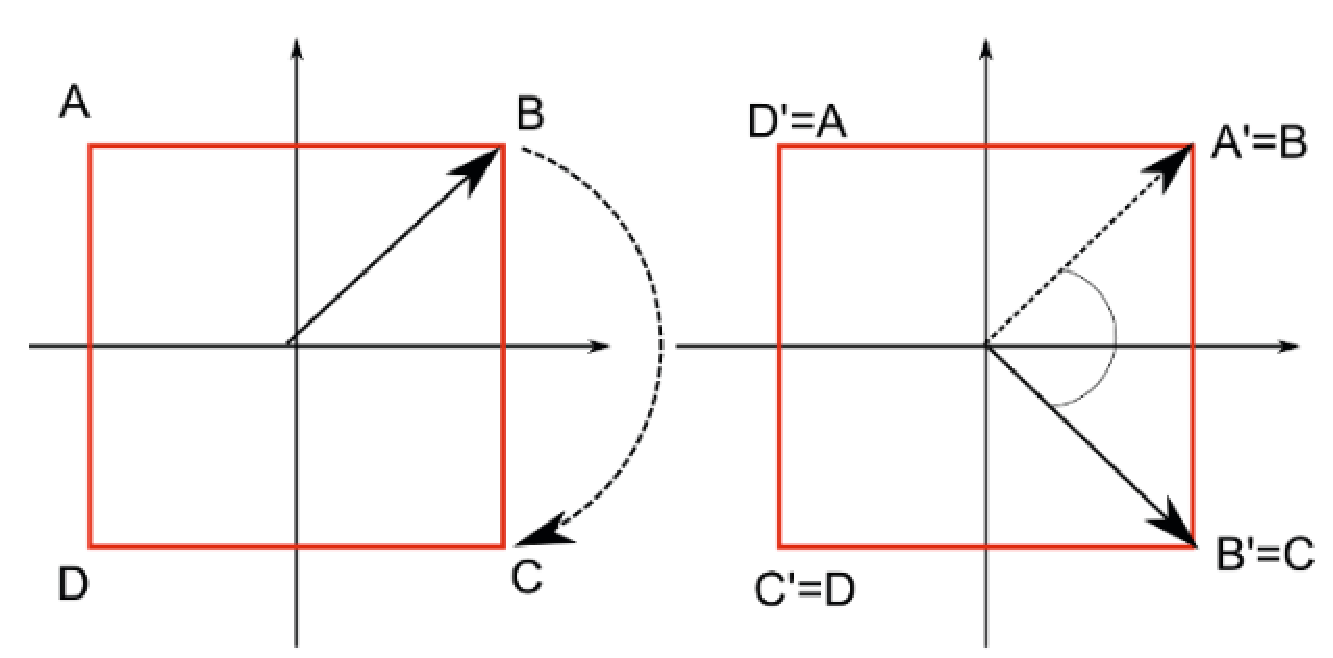
\includegraphics[scale=0.4]{fig3_3}
	\caption{正方形绕中心旋转$90^\circ$}
	\label{fig3.3}
	}

	换个角度看:假如你看了一眼原来的正方形, 然后闭上眼睛, 这时有人可能把正方形做了一个变换。 如果你睁眼以后不能分辨这个正方形是否被人变换过, 那么这个变换就是个对称变换。

	我们把所有使正方形不变的变换构成的集合称为群。 变换参数(本例中就是旋转角度)不能任意取值(而是取分立的数), 这样这个群称为离散群。

	\item 另一个例子是使单位圆不变的变换构成的集合。 类似地, 单位圆还是一些点构成的集合, 对称变换把这个集合映射到它自身。

	单位圆绕圆心旋转任意角度都不变。 换言之, 变换参数(这里就是旋转角度)可以取任意值, 因此这个群是连续群。
\end{enumerate}
	\picmpar{
		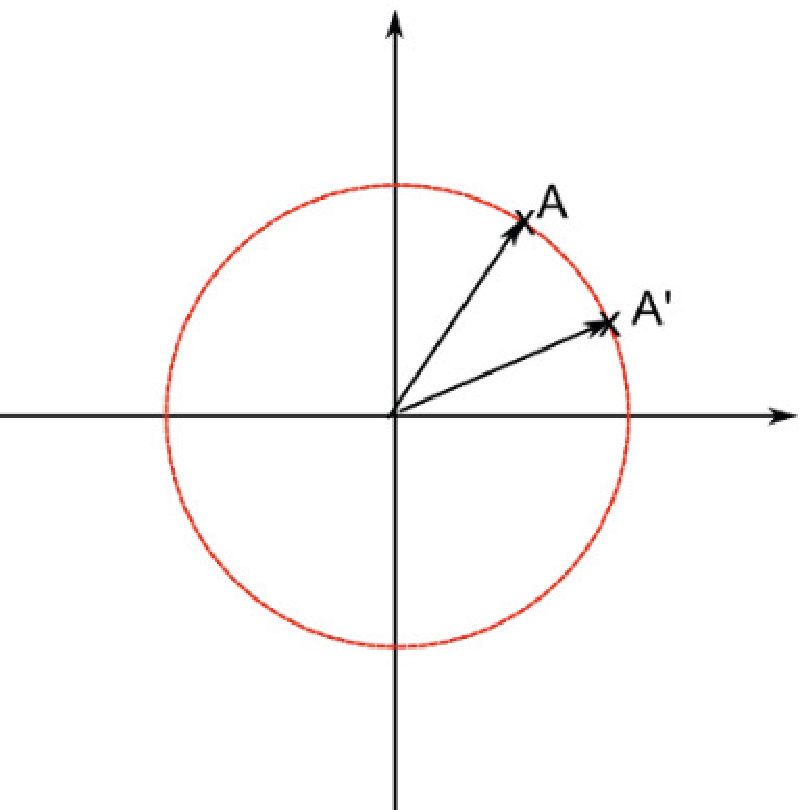
\includegraphics[scale=0.35]{fig3_4.pdf}
		\caption{单位圆旋转的示意图,单位圆绕圆心旋转任意角度都不变}
	}

数学中除了几何图形之外还有好多别事物的都有对称性。 例如,对于向量, 我们可以考虑所有让向量长度不变的变换构成的集合。 看出本节开头对称性定义的普遍性了没? 对称性就是变换下的不变性。 非常幸运, 搞数学的早已建立了群论, 它可以研究所有类型的对称性\mpar{历史上数学家们建立群论最初是为了描述方程的对称性}。

为了让描述对称的工具——群——有确切的含义, 我们把对称性的定义用数学语言精炼一下:
\begin{itemize}
	\item 对某物什么也不做(比如转个$0^\circ$)当然也是对称变换(按照我们的对称性定义), 因此任何群都需要包含一个恒等变换(恒等元)。 在上面的例子里, 恒等元就是旋转$0^\circ$。

	\item 对某物先做变换再做逆变换的结果必须等于啥也不做。 因此对于群中的任意元素(简称群元), 必须有相应的逆元素。 按定义, 先做变换再做逆变换等于恒等变换。 例如先转$90^\circ$再转$-90^\circ$(先逆针再顺针转)与旋转$0^\circ$相同。

	\item 先做一个对称变换再做一个对称变换, 总体效果必须还是对称变换。 例如先旋转$90^\circ$再转$180^\circ$等于直接转$270^\circ$, 后者也是对称变换。 对称变换的这个性质称为封闭性。

	\item 对称变换之间必须满足结合律\mpar{它们不一定满足交换律!例如绕不同轴的旋转变换之间不能交换顺序,比如$R_x(\theta) R_z(\phi) \neq R_z(\phi) R_x(\theta)$}。 例如转$90^\circ$再转$40^\circ$再转$110^\circ$这种操作,无论是先转$130^\circ$再转$110^\circ$,还是先转$90^\circ$再转$150^\circ$都一样。 用符号表示更加清楚:
	\begin{equation}\label{equ3.1}
	R(110^\circ) R(40^\circ) R(90^\circ) = R(110^\circ)\bigg( R(40^\circ)R(90^\circ) \bigg) = R(110^\circ) R(130^\circ)
	\end{equation}
	\begin{equation}\label{equ3.2}
	R(110^\circ) R(40^\circ) R(90^\circ) = \bigg( R(110^\circ) R(40^\circ) \bigg) R(90^\circ) = R(150^\circ) R(90^\circ)
	\end{equation}
	这个性质称为{\bfseries 结合律}。

	\item 我们需要了解两个群元(对称变换)是怎样结合的。这种结合是个{\bfseries 二元运算}\footnote{两个群元结合成一个}, 我们称它为{\bfseries 群乘法}。
\end{itemize}

	在上面的例子里, 旋转变换的标准表示方法是用旋转矩阵\mpar{旋转矩阵见附录\ref{appendix.A.2}。}, 两个群元(两个旋转矩阵, 或两个旋转操作)结合的规则是线性代数里的矩阵乘法。 同样的变换经常有不同的表示方法\mpar{例如, 二维平面旋转还可以用单位复数描述, 相应的群乘法是复数乘法。 稍后就讨论这一点。}, 群论非常系统性地概括了所有形式。 群论的分支——{\bfseries 表示论}就是研究相同变换的不同描述方式的, 我们在\ref{sec3.5}节学习表示论。

\

我们把上述群与对称变换的特征用严谨的数学语言表达, 再将它们提升为公理, 满足这些公理的一切数学结构就称为群。必须指出我们可以搞出超级抽象而又满足群公理的结构, 但我们现在只关注上面例子里的旋转变换那样的群。

讨论完了这些,我们认识到群的抽象定义仅仅是(显然地)蕴含着这些(我们通过对称变换的性质导出的)群公理的东西\mpar{别担心怎么才能根据这些公理凑出一个群来。 搞物理的往往是从某个变换出发, 考察它是否符合群公理, 如果是那么就可以应用群论来解决问题。}:

一个群是一个集合$G$,加上一个定义在$G$上的二元运算(群乘法)$\circ$, 且要求$(G, \circ)$满足以下公理:
\begin{itemize}
	\item 封闭性: 对于任意$g_1, g_2 \in G, g_1 \circ g_2 \in G$

	\item 单位元: 存在单位元$e \in G$使得对于所有$g \in G, g\circ e = g = e \circ g$

	\item 逆元: 对于任意$g \in G$, 存在相应的逆元$g^{-1} \in G$使得$g \circ g^{-1} = e = g^{-1} \circ g$

	\item 结合律: 对于任意$g_1, g_2, g_3 \in G, g_1 \circ (g_2 \circ g_3) = (g_1 \circ g_2) \circ g_3$
\end{itemize}

总而言之: 某对象在一些变换下保持不变, 所有的这些变换组成\footnote{我在想这里该用`构成'还是`组成', 后来我觉得无所谓, 因为这不是初中化学...(分子构成物质, 元素组成物质...)——译者(SI)}的集合叫做对称群。 对于Minkowski时空, Minkowski度规\mpar{复习一下, Minkowski度规就是在Minkowski空间中用来计算距离和长度的工具, 见第\ref{chap2}章。}在变换下保持不变, 相应的对称群称为Poincar\'e群。

要注意群的定义完全与变换的对象是啥没有关系。 因此我们可以脱离特定对象而只研究对称变换本身, 群的定义将变换从对象中`提取'出来了。 这是非常有用的, 许多不同事物具有同样或同类的对称性。 群论让我们不用管变换的对象\footnote{译者注:圆还是正方形}, 只研究变换(例如旋转)的普遍性质。


\section[二维旋转]{Rotations in two Dimensions\quad 二维旋转}
\label{sec3.2}
我们从一个简单而重要的例子开始学习群论。考虑那些让二维平面中的向量长度不变的对称变换。符合条件的有旋转和反射\mpar{当然还有平移。平移的数学描述与前两者有些不同,我们之后再讨论它。}。它们也是圆的对称变换,一个单位元旋转或反射之后还是单位圆。可见同一个群(对应一种变换)可以作用于不同类对象:圆(几何图形),或者向量\footnote{可以简单考虑为一个点,其相对于原点就是该向量。——译者注}。本节考虑向量,可以用旋转矩阵表示向量的旋转或反射\mpar{旋转矩阵的推导见附录\ref{appendix.A.2}。},将起点位于原点的向量绕原点逆时针旋转$\theta$角度的旋转矩阵为\footnote{译者注:原文此式符号有误。}
\begin{equation}
\label{equ3.3}
R_\theta =
	\begin{pmatrix}
		\cos \theta & -\sin \theta \\
		\sin \theta & \cos \theta
	\end{pmatrix}
\end{equation}

关于$x$轴与$y$轴的反射变换用矩阵表示为:
\begin{equation}
\label{equ3.4}
P_x = 	\begin{pmatrix}
			-1 & 0 \\ 0 & 1
		\end{pmatrix}
\quad
P_y = 	\begin{pmatrix}
			1 & 0 \\ 0 & -1
		\end{pmatrix}
\end{equation}
将矩阵乘法作为群乘法$\circ$, 可以验证对于所有的$\theta$,$R(\theta), P_x, P_y$与矩阵乘法符合群公理,因而构成一个群,亦即旋转与反射变换构成一个群。

可以用更抽象的方式表达‘所有让二维向量长度不变的变换’,向量长度就是向量与自身点乘的平方根($|a| = \sqrt{a \cdot a}$). 向量长度在变换$a \rightarrow a'$下不变意味着\footnote{等号上面的!只是起强调、提示作用——译者(SI)}:
\begin{equation}
\label{equ3.5}
a' \cdot a' \stackrel{!}{=} a \cdot a
\end{equation}

将线性变换对应的矩阵记作$\mathcal{O}$,变换即为$a \rightarrow a' = \mathcal{O}a$.
\begin{equation}
\label{equ3.6}
a \cdot a = a^{{T}} a \rightarrow a'^{{T}} a' = (\mathcal{O} a)^{{T}} \mathcal{O} a = a^{{T}} \mathcal{O}^{{T}} \mathcal{O} a \stackrel{!}{=} a^{{T}} a = a \cdot a
\end{equation}
由此可见,使向量长度不变的变换必须满足\footnote{其中是由于$a$任意从而能够得到$\mathcal{O}^{{T}} \mathcal{O} = I$。}:
\begin{equation}
\label{equ3.7}
\mathcal{O}^{{T}} \mathcal{O} = I
\end{equation}
其中$I$表示单位矩阵。\mpar{ \[I =
	\begin{pmatrix}
		1 & 0 \\ 0 & 1
	\end{pmatrix}\]}。前文的旋转和反射矩阵都满足此条件\mpar{例如\eqref{equ3.3}式的矩阵,
	$R_\theta^{{T}} R =
	\begin{pmatrix}
		\cos \theta & -\sin \theta \\
		\sin \theta & \cos \theta
	\end{pmatrix}
	\begin{pmatrix}
		\cos \theta & \sin \theta \\
		-\sin \theta & \cos \theta
	\end{pmatrix}
	 =
	 \begin{pmatrix}
		 \cos^2 \theta + \sin^2 \theta & 0 \\
		 0 & \sin^2 \theta + \cos^2 \theta
	 \end{pmatrix}
	 =
	 \begin{pmatrix}
		 1 & 0 \\ 0 & 1
	 \end{pmatrix}
	$
}%mpar
$2 \times 2$矩阵中所有满足\eqref{equ3.7}式的矩阵构成了$\mathcal{O}(2)$群,即所有$2 \times 2$正交矩阵构成的群\mpar{严谨地说,任意$2 \times 2$正交矩阵可以表示为\eqref{equ3.3}、\eqref{equ3.4}式,或者它们的乘积的形式。}。我们可以找出这个群中描述旋转变换的那一部分(构成一个子群)。根据\eqref{equ3.7}式:
\begin{align}
\det(\mathcal{O}^{{T}} O ) = \det(O^{{T}}) \det(O) \stackrel{!}{=} \det(I) = 1 \nonumber\\
\label{equ3.8}
(\det(\mathcal{O}))^2 \stackrel{!}{=} 1 \rightarrow \det{(\mathcal{O})} \stackrel{!}{=} \pm 1
\end{align}

$\det \mathcal{O} = 1$的矩阵对应旋转变换\mpar{见\eqref{equ3.3}与\eqref{equ3.4}式。反射矩阵的行列式等于$-1$。}。
而条件
\begin{align}
\label{equ3.9}
\mathcal{O}^{{T}} \mathcal{O} = I \\
\label{equ3.10}
\det \mathcal{O} = 1
\end{align}
定义了$\mathcal{SO}(2)$群,这里的$\mathcal{S}$表示‘特殊’(special),$\mathcal{O}$表示‘正交’(orthogonal)。

$\mathcal{SO}(2)$包含的旋转变换保持了坐标系的取向,即一个右手坐标系\mpar{右手坐标系与左手坐标系见附录\ref{appendix.A.5}。}经旋转变换后还是右手系,而反射变换会改变它的取向。用线性代数的概念来说,我们规定$\mathcal{SO}(2)$中的矩阵行列式必须为$+1$。

\subsection[用单位复数表示旋转变换]{Rotations with Unit Complex Numbers\quad 用单位复数表示旋转变换}
\label{sec3.2.1}
还可以用单位复数来表示二维的旋转变换:绕原点旋转$\theta$角可以表示为乘以单位复数$z$(单位复数意为$z = a + ib$,$|z|^2 = z^* z = 1$)\mpar{上标$ ^*$表示复数的共轭复数:$z = a + ib \rightarrow z^* = a - ib$}。

所有单位复数构成一个群,称为\mpar{$\mathcal{U}$表示幺正性,它的含义为$\mathcal{U}^* \mathcal{U} = 1$.}\ $\mathcal{U}(1)$,群乘法即为复数乘法,不难验证它符合群公理。为了看出它与之前引入的$\mathcal{O}(2), \mathcal{SO}(2)$群\footnote{译者注:原文有误,现已更正}的关系,我们将$\mathcal{U}(1)$群的条件——复数的模(长度)为1表示为\mpar{定义中包含复数乘法的群的普遍性质见\ref{sec3.10}节的附录。}, $\forall \mathcal{U} \in \mathcal{U}(1)$:
\begin{equation}
\label{equ3.11}
\mathcal{U}^* \mathcal{U} = 1
\end{equation}
单位复数另一种写法是\mpar{附录\ref{appendix.B.4.2}推导了传说中的欧拉公式。对任意复数$z = a + ib$, $a$称为$z$的实部,记为$\mathrm{Re}(z) = a$; $b$称为虚部,记为$\mathrm{Im}(z) = b$. 欧拉公式中$R_\theta$的实部为$\cos  \theta$, 虚部为$\sin \theta$.}:% Euler翻译为欧拉
\begin{equation}
\label{equ3.12}
R_\theta = \mathrm{e}^{i\,\theta} = \cos \theta + i\sin \theta
\end{equation}
$R_\theta$的模平方为:
\begin{equation}
\label{equ3.13}
R_\theta^* R_\theta = \mathrm{e}^{-i\,\theta} \mathrm{e}^{i\,\theta} = \big( \cos \theta - i \sin \theta  \big) \big( \cos \theta + i \sin \theta \big) = 1
\end{equation}

\picmpar{
	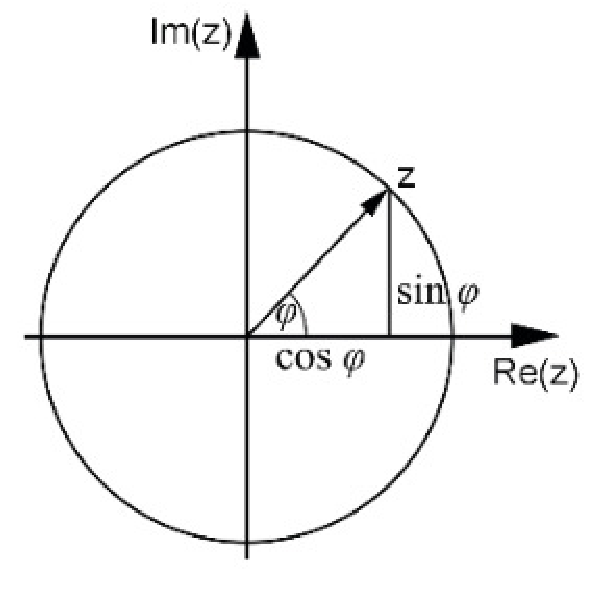
\includegraphics[scale=0.45]{fig3_5.pdf}
	\caption{单位复数在复平面的单位圆上}
	\label{fig3.5}
	}

例:将向量$(3,  5)$对应的复数$z = 3 + 5i$旋转$90^\circ$:
\begin{equation}
\label{equ3.14}
z \rightarrow z' = \mathrm{e}^{i\, 90^\circ}z = \bigg( \underbrace{\cos 90^\circ}_{=0} + i\underbrace{\sin 90^\circ}_{=1} \bigg) (3 + 5i) = i(3 + 5i) = 3i - 5
\end{equation}

图\ref{fig3.6}绘制了旋转前后的向量(复数),图中可见复数乘以$\mathrm{e}^{i\, 90^\circ}$旋转了$90^\circ$.
\picmpar{
	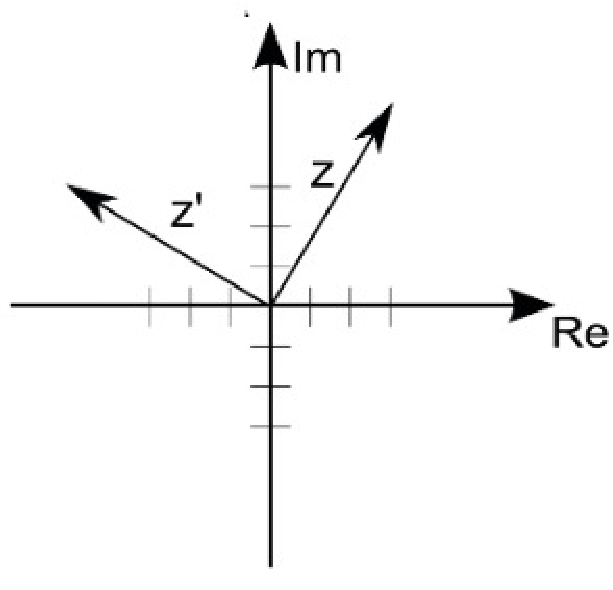
\includegraphics[scale=0.45]{fig3_6.pdf}
	\caption{复数通过乘以单位复数进行旋转}
	\label{fig3.6}
	}

需要注意$\mathrm{e}^{i\, 90^\circ}$作用于(乘以)向量对应的复数而非向量本身。描述二维旋转只需要一个参数:旋转角$\phi$. 而复数有两个自由度(实部和虚部),因此我们加上单位复数的限制:$|z| = \text{实部}^2 + \text{虚部}^2 = 1$,刚好只剩一个自由度。

描述二维旋转的两种方式——单位复数与$2 \times 2$矩阵(矩阵元都是实数)通过如下方式相联系。定义:
\begin{equation}
\label{equ3.15}
\mathbf{1} =
	\begin{pmatrix}
		1 & 0 \\ 0 & 1
	\end{pmatrix}
,\quad
\mathbf{i} =
	\begin{pmatrix}
		0 & -1 \\ 1 & 0
	\end{pmatrix}
\end{equation}
不难验证这样定义的$\mathbf{1, i}$仍然满足:
\begin{equation}
\mathbf{1}^2 = \mathbf{1},\quad \mathbf{i}^2 = -\mathbf{1},\quad \mathbf{1i} = \mathbf{i1} = \mathbf{i}
\end{equation}
这样单位复数对应的$2 \times 2$实数矩阵为\footnote{译者注:原文此式有误,译文已参照勘误表修改。}
\begin{equation}
\label{equ3.17}
R_\theta = \cos \theta + i\sin\theta = \cos \theta
\begin{pmatrix}
	1 & 0 \\ 0 & 1
\end{pmatrix}
+ \sin \theta
\begin{pmatrix}
	0 & -1 \\ 1 & 0
\end{pmatrix}
=
\begin{pmatrix}
	\cos \theta & -\sin \theta \\
	\sin \theta & \cos \theta
\end{pmatrix}
\end{equation}
可见,定义了复单位$i \rightarrow \text{实矩阵}$的对应关系后,单位复数就回到了熟悉的旋转矩阵。还有一点要注意:旋转矩阵作用于向量(列矩阵),而我们将$i$与$2 \times 2$的实矩阵相联系,因此被旋转的向量(与一个复数对应)也将变成一个$2 \times 2$矩阵。

例:任意向量$(a, b)$对应的复数对应的$2 \times 2$矩阵为:
\begin{equation}
\label{equ3.18}
z = a + ib = a
\begin{pmatrix}
	1 & 0 \\ 0 & 1
\end{pmatrix}
+ b
\begin{pmatrix}
	0 & -1 \\ 1 & 0
\end{pmatrix}
=
\begin{pmatrix}
	a & -b \\ b & a
\end{pmatrix}
\end{equation}
将旋转矩阵作用于$z$:
\begin{eqnarray}
\label{sec3.19}
	z' &=& \begin{pmatrix}
			a' & -b' \\ b' & a'
		 \end{pmatrix}
	= R_\theta z =
		\begin{pmatrix}
			\cos \theta & -\sin \theta \\
			\sin \theta & \cos \theta
		\end{pmatrix}
		\begin{pmatrix}
			a & -b \\ b & a
		\end{pmatrix}
	\nonumber \\
	&=& \begin{pmatrix}
			a\cos\theta - b\sin \theta & - b\cos \theta - a \sin \theta \\
			a\sin \theta + b\cos \theta & -b \sin \theta + a \cos \theta
		\end{pmatrix}
\end{eqnarray}
由上式可得
\begin{align}
\label{equ3.20}
a' &= a \cos \theta - b \sin \theta \\
\label{equ3.21}
b' &= a \sin \theta + b \cos \theta
\end{align}
这与旋转矩阵作用于向量(列矩阵形式)相同:
\begin{equation}
\label{equ3.22}
	\begin{pmatrix}
		\cos \theta & -\sin \theta \\
		\sin \theta & \cos \theta
	\end{pmatrix}
	\begin{pmatrix}
		a \\ b
	\end{pmatrix}
	=
	\begin{pmatrix}
		a \cos \theta - b \sin \theta \\
		a \sin \theta + b \cos \theta
	\end{pmatrix}
	=
	\begin{pmatrix}
		a' \\ b'
	\end{pmatrix}
\end{equation}
我们看到这两种表示方法是一回事儿,用数学术语来说,$\mathcal{SO}(2)$与$\mathcal{U}(1)$间有一个同构映射\mpar{如果映射$\Pi: G \rightarrow G'$是一一映射,并且满足:$\forall g_1, g_2 \in G, \Pi(g_1) \circ \Pi(g_2) = \Pi(g_1 \circ g_2)$, 则$\Pi$就是同构映射,并且称群$G, G'$是同构的。}。这一点太重要了,之后的篇幅会不断出现这种思想。

下面研究三维旋转,尝试找出它的两种描述方法\mpar{其中蕴含着十分硬却失挺(interesting)的内容... 与二维旋转类似,我们将找出三维旋转的第二法,这个第二法能够揭示大自然更深刻的内容。}。

\section[三维旋转]{Rotations in three Dimensions\quad 三维旋转}
\label{sec3.3}
三维向量旋转变换当然可以用$3 \times 3$旋转矩阵\footnote{原文公式有误,译文已按勘误表改正。}:
\begin{align}
R_x =
	\begin{pmatrix}
		1 & 0 & 0 \\
		0 & \cos \theta & -\sin \theta \\
		0 & \sin \theta & \cos \theta
	\end{pmatrix}
\quad
R_y =
	\begin{pmatrix}
		\cos \theta & 0 & \sin \theta \\
		0 & 1 & 0 \\
		-\sin \theta & 0 & \cos \theta
	\end{pmatrix}
\nonumber \\
\label{equ3.23}
R_z =
	\begin{pmatrix}
		\cos \theta & -\sin \theta & 0 \\
		\sin \theta & \cos \theta & 0 \\
		0 & 0 & 1
	\end{pmatrix}
\end{align}

类比$\mathcal{SO}(2)$群,上面三个矩阵构成了$\mathcal{SO}(3)$群的一组基\mpar{基的概念见附录\ref{appendix.A.1}。}。这意味着$\mathcal{SO}(3)$中的任意群元(矩阵)都可以写为$R_x, R_y, R_z$的线性组合,且系数唯一。
将向量
\begin{equation*}
\vec{v} = \begin{pmatrix}
			1 \\ 0 \\ 0
		\end{pmatrix}
\end{equation*}
绕$z$轴旋转\mpar{三维向量旋转的一般情况的推导见附录\ref{appendix.A.2}。}就是用旋转矩阵乘以向量:
\begin{equation}
\label{equ3.24}
R_z(\theta) \vec{v} =
	\begin{pmatrix}
		\cos \theta & -\sin \theta & 0 \\
		\sin \theta & \cos \theta & 0 \\
		0 & 0 & 1
	\end{pmatrix}
	\begin{pmatrix}
		1 \\ 0 \\ 0
	\end{pmatrix}
=
	\begin{pmatrix}
		\cos \theta \\ \sin \theta \\ 0
	\end{pmatrix}
\end{equation} \footnote{译者注:原文符号有误,现已订正。}
为找出描述三维旋转的第二法,我们尝试把复数的概念扩展到三维空间。首先试着把$2$维的复数\footnote{实部虚部两个自由度}扩展为$3$维复数,但前人探索发现没有$3$维的,但存在$4$维‘复数’,称为{\bfseries 四元数(quaternions)}。下面就会看到四元数正是描述三维旋转的第二法,并且它还能深刻揭示宇宙——四维时空的规律。描述三维旋转需要三个参数(绕$x,y,z$轴的旋转角),而四元数有四个参数,这与二维旋转的情况类似\mpar{单位复数描述二维旋转。}。四元数加上单位长度的限制——单位四元数(三个自由参数)能够描述三维旋转。

\subsection[四元数]{Quaternions\quad 四元数}
\label{sec3.3.1}
我们类比复数来构造四元数,复数只有一个虚单位$i$,而四元数里定义三个虚单位,记作$\mathbf{i,j,k}$,它们仍然满足
\begin{equation}
\label{equ3.25}
\mathbf{i}^2 = \mathbf{j}^2 = \mathbf{k}^2 = -1
\end{equation}
这样任意一个四元数$q$表示为
\begin{equation}
\label{equ3.26}
q = a\mathbf{1} + b\mathbf{i} + c\mathbf{j} + d\mathbf{k}
\end{equation}
其中$a, b, c, d \in \mathbb{R}$, $\mathbf{1}$就是正常的实数1。\footnote{$\mathbf{1,i,j,k}$用黑体表示是为了强调它们是四元数的基。---译者(SI)}

要想定义四元数间的乘法,必须定义虚单位间的乘法规则,比如$\mathbf{ij} = ?$. 为此再定义
\begin{equation}
\label{equ3.27}
\mathbf{ijk} = -1
\end{equation}
这样虚单位间的乘法就没问题了,例如,为导出$\mathbf{ij} = \mathbf{k}$, 在\eqref{equ3.27}式等号两侧右乘$\mathbf{k}$:
\begin{equation}
\label{equ3.28}
\mathbf{ij} \underbrace{\mathbf{kk}}_{= -1} = -\mathbf{k} \rightarrow \mathbf{ij} = \mathbf{k}
\end{equation}

单位四元数$q = a\mathbf{1} + b\mathbf{i} + c\mathbf{j} + d\mathbf{k}$满足\mpar{符号$\dag$称为`dagger',表示转置加取复共轭,即$a^\dag = (a^*)^T$。实数向量间的点乘定义为$a \cdot b = a^T b$, 向量用列矩阵表示,其转置为行矩阵,于是点乘的定义符合矩阵乘法规则。四元数对应的列矩阵含复数,为使四元数与它自身相乘结果为实数(实数结果可表示‘长度’),在转置之外还加上取复共轭。}:
\begin{align}
q^\dag q &\stackrel{!}{=} 1 \nonumber\\
\label{equ3.29}
\rightarrow (a\mathbf{1} - b\mathbf{i} - c\mathbf{j} - d\mathbf{k}) (a\mathbf{1} +& b\mathbf{i} + c\mathbf{j} + d\mathbf{k}) = a^2 + b^2 + c^2 + d^2 \stackrel{!}{=} 1
\end{align}

就像单位复数构成一个群(群乘法为复数乘法)那样,单位四元数也构成一个群(群乘法为四元数乘法)。

类似于我们将二维复数与$2 \times 2$实数矩阵建立联系的做法,四元数也可如此——将四个基$\mathbf{1,i,j,k}$与合适的矩阵一一对应。其中一种方式(还有别的方式)是将它们与$2 \times 2$复数矩阵对应\footnote{译者注:原文此式及后续\eqref{equ3.31}、\eqref{equ3.38}、\eqref{equ3.39}、\eqref{equ3.43}和\eqref{equ3.44}均有误,已据勘误表订正。}:
\begin{align}
\mathbf{1} = \begin{pmatrix}
				1 & 0 \\ 0 & 1
			 \end{pmatrix}
\quad &, \quad
\mathbf{i} = \begin{pmatrix}
				0 & -1 \\ 1 & 0
			 \end{pmatrix}
\nonumber \\
\label{equ3.30}
\mathbf{j} = \begin{pmatrix}
				0 & i \\ i & 0
			 \end{pmatrix}
\quad &, \quad
\mathbf{k} = \begin{pmatrix}
				i & 0 \\
				0 & -i
			 \end{pmatrix}
\end{align}
不难验证上式满足四元数乘法,比如\eqref{equ3.25}、\eqref{equ3.27}式。这样任意一个四元数都可用矩阵表示为:
\begin{equation}
\label{equ3.31}
q = a\mathbf{1} + b\mathbf{i} + c\mathbf{j} + d\mathbf{k} = \begin{pmatrix}
	a + di & b + ci \\
	- b + ci & a - di
	\end{pmatrix}
\end{equation}
由上式可见
\begin{equation}
\label{equ3.32}
\det(q) = a^2 + b^2 + c^2 + d^2
\end{equation}
上式与\eqref{equ3.29}式比较可以发现单位四元数对应的矩阵的行列式为$1$。因此单位四元数对应的$2 \times 2$复数矩阵$\mathcal{U}$满足:
\begin{equation}
\label{equ3.33}
\mathcal{U}^\dag \mathcal{U} = 1, \quad \text{且} \det(\mathcal{U}) = 1
\end{equation}
注意\eqref{equ3.30}式中的矩阵是线性独立的\mpar{线性独立的概念见附录\ref{appendix.A.1}。},它们构成群$\mathcal{SU}(2)$的基。与之前相同,$\mathcal{S}$表示特殊(special),含义为$\det (\mathcal{U}) = 1$;$\mathcal{U}$表示幺正(unitary)\mpar{进一步介绍见本章附录\ref{sec3.10}节。},即$\mathcal{U}^\dag \mathcal{U} = 1$。任意单位四元数都唯一对应$\mathcal{SU}(2)$群中的一个群元。

$\mathcal{SU}(2)$群如何与三维旋转联系?和之前不同,$\mathcal{SU}(2)$群与$\mathcal{SO}(3)$\mpar{$\mathcal{SO}(3)$群就是三维旋转矩阵构成的群。}之间的对应关系并不像二维旋转中$\mathcal{U}(1)$与$\mathcal{SO}(2)$那样简单。

2维虚数$z = a + ib$与2维向量很容易对应。单位复数保证了矢量长度在旋转变换下不变\mpar{注意这里的$R$表示一个单位复数,即$R^* R = 1$, $R$与复数$z$相乘就将$z$进行旋转变换。}:$(Rz)^* Rz = z^* R^* Rz = z^* z$。四元数有$4$个参数,它与三维向量的对应关系是并不明显。我们尝试将三维向量$\vec{v} = (x, y, z)$定义为如下四元数\footnote{注意下式中的$\mathbf{ijk}$是四元数的‘基’而非三维直角坐标系的基矢。——译者}:
\begin{equation}
\label{equ3.34}
v \equiv x\mathbf{i} + y\mathbf{j} + z\mathbf{k}
\end{equation}
利用前述四元数的矩阵表示可得:
\begin{equation}
\label{equ3.35}
\det(v) = x^2 + y^2 + z^2
\end{equation}
于是保持向量$(x, y, z)$长度不变的变换就对应于保持矩阵行列式不变的矩阵变换。而{\bfseries 单位}四元数对应矩阵都具有{\bfseries 单位}行列式,它与任意矩阵相乘不改变该矩阵的行列式\footnote{利用$\det(AB) = \det(A)\det(B)$,——译者}。进展很顺利,但现在有个微妙的状况:继续猜想下去,我们会认为用单位四元数$u$旋转向量(对应的四元数)$v$直接用$u$乘以$v$就可以了(按照四元数乘法规则)。但细想起来这却不行,因为根据\eqref{equ3.34}式,我们把任意三维向量对应的四元数定义在$\mathbb{R}\mathbf{i} + \mathbb{R}\mathbf{j} + \mathbb{R}\mathbf{k}$的范围内,$u$与$v$的四元数乘积会超出这个范围,这样向量旋转后可能不是个向量!这当然不行。

事实上,旋转变换表示为:
\begin{equation}
\label{equ3.36}
v' = q^{-1} v q
\end{equation}
其中$v$, $v'$分别为旋转前后的向量,$q$为表示旋转的单位四元数。

这样我们终于实现了描述三维旋转的第二法——单位四元数。

例:定义$u$是$\mathbb{R}\mathbf{i} + \mathbb{R}\mathbf{j} + \mathbb{R}\mathbf{k}$中的某一单位向量,则任意单位四元数$t$可表示为:
\begin{equation}
\label{equ3.37}
t = \cos \theta +  u\sin \theta
\end{equation}
利用\eqref{equ3.34}式,任意三维向量$\vec{v}$可表示为:
\begin{equation}
\label{equ3.38}
\vec{v} = (v_x, v_y, v_z)^T = v_x \mathbf{i} + v_y \mathbf{j} + v_z \mathbf{k} \underbrace{=}_{\eqref{equ3.31}\text{式}} \begin{pmatrix}
		iv_z & v_x + iv_y \\
		-v_x + iv_y & -iv_z
	\end{pmatrix}
\end{equation}

简明起见我们举个特例,把向量$\vec{v} = (1, 0, 0)^T$绕$z$轴旋转。
\begin{align}
\label{equ3.39}
\vec{v} &= (1, 0, 0)^T \rightarrow v = 1\mathbf{i} + 0\mathbf{j} + 0\mathbf{k} =
	\begin{pmatrix}
		0 & 1 \\ -1 & 0
	\end{pmatrix}
\\
\label{equ3.40}
R_z(\theta) &= \cos \theta \mathbf{1} + \sin \theta \mathbf{k} =
	\begin{pmatrix}
		\cos \theta + i\sin \theta & 0 \\
		0 & \cos \theta - i\sin \theta
	\end{pmatrix}
\end{align}
上式也可用欧拉公式写出\mpar{欧拉公式的推导见附录\ref{appendix.B.4.2}}:
\begin{equation}
\label{equ3.41}
\mathrm{e}^{ix} = \cos x + i\sin x
\Rightarrow
R_z(\theta) = \begin{pmatrix}
				\mathrm{e}^{i\theta} & 0 \\
				0 & \mathrm{e}^{-i\theta}
			  \end{pmatrix}
\end{equation}
四元数旋转矩阵的逆矩阵为:
\begin{equation}
\label{equ3.42}
R_z^{-1} (\theta) =
	\begin{pmatrix}
		\cos \theta - i\sin \theta & 0 \\
		0 & \cos \theta + i\sin \theta
	\end{pmatrix}
=
	\begin{pmatrix}
		\mathrm{e}^{-i\theta} & 0 \\
		0 & \mathrm{e}^{i\theta}
	\end{pmatrix}
\end{equation}
根据\eqref{equ3.36}式旋转向量$v$;
\begin{align}
v' &= R_z^{-1} (\theta) v R_z(\theta) =
	\begin{pmatrix}
		\mathrm{e}^{-i\theta} & 0 \\
		0 & \mathrm{e}^{i\theta}
	\end{pmatrix}
	\begin{pmatrix}
	0 & 1 \\ -1 & 0
	\end{pmatrix}
	\begin{pmatrix}
		\mathrm{e}^{i\theta} & 0 \\
		0 & \mathrm{e}^{-i\theta}
	\end{pmatrix}
\nonumber \\
\label{equ3.43}
&= \begin{pmatrix}
		0 & \mathrm{e}^{-i 2\theta} \\
		-\mathrm{e}^{i 2\theta} & 0
	\end{pmatrix}
= \begin{pmatrix}
		0 & \cos (2\theta) - i\sin (2\theta) \\
		-\cos (2\theta) - i\sin (2\theta) & 0
  \end{pmatrix}
\end{align}
另一方面,向量$v'$用四元数表示为:
\begin{equation}
\label{equ3.44}
v' =
	\begin{pmatrix}
		iv'_z & v'_x + iv'_y \\
		-v'_x + iv'_y & -iv'_z
	\end{pmatrix}
\end{equation}
上式与\eqref{equ3.43}式比较可得:
\begin{equation}
\label{equ3.45}
v'_x = \cos(2\theta),\quad v'_y = -\sin (2\theta),\quad v'_z = 0
\end{equation}
所以
\begin{equation}
\label{equ3.46}
\rightarrow \vec{v'} = \big( \cos(2\theta), -\sin (2\theta), 0 \big)^T
\end{equation}
由上式可见从$\vec{v}$到$\vec{v}'$确实进行了旋转\mpar{见\eqref{equ3.24}式,那里我们用三维旋转矩阵旋转向量。},但是要注意,上式表示我们没有把$\vec{v}$旋转$\theta$角度,而是旋转了$2\theta$!因此我们定义$\phi \equiv 2 \theta$, 这样$\phi$表示真正的旋转角,$\eqref{equ3.37}$重写为:
\begin{equation}
\label{equ3.47}
t = \cos \left( \frac{\phi}{2} \right) + \sin \left(\frac{\phi}{2} \right) u
\end{equation}

这样定义的单位四元数与三维旋转矩阵之间的关系并非一一对应的,而是两个单位四元数描述同一个旋转,例如\mpar{将向量旋转$\pi$与旋转$3\pi = \pi + 2\pi$相同。换言之:两个单位四元数$u$与$-u$对应同一变换:旋转$\pi$.}:

{
\centering
\setlength{\unitlength}{0.8cm}
\begin{picture}(6, 4.5)\thicklines
\put(0.5, 3){\makebox(2.5, 1.2){\text{$t_{\phi = \pi} = u$}}}
\put(5.5, 3){\makebox(2.5, 1.2){\text{$t_{\phi = 3\pi} = -u$}}}

\put(1.7, 3.2){\vector(1, -1){1.4}}
\put(6.0, 3.2){\vector(-1, -1){1.4}}
\put(2.8, 0.8){\makebox(2.5, 1.2){\text{将向量旋转$\pi$}}}
\end{picture}
}

因此$\mathcal{SU}(2)$群称为$\mathcal{SO}(3)$群的{\bfseries 双覆盖}。一个$\mathcal{SU}(2)$中的群元对应$\mathcal{SO}(3)$的哪个群元是很明确的,反过来就不行,因为$\mathcal{SO}(3)$中的一个群元对应$\mathcal{SU}(2)$中的两个。这并非仅有数学意义,稍后就会看到,在物理上,一个能覆盖别的群的群往往更加深刻\mpar{剧透:Lorentz群的双覆盖蕴含{\bfseries 自旋}概念,而Lorentz群自身并不具有。自旋是指粒子的某种内禀角动量,它是粒子最重要的特征之一。自旋在小节\ref{sec4.5.4}和\ref{sec8.5.5}详述。}。

给定某个群,为了找出能覆盖这个群的群,我们需要学习Lie代数——Lie理论的利器,下一节就讲Lie代数。

注意我们把三维向量对应到四元数集$\mathbb{R}\mathbf{i} + \mathbb{R}\mathbf{j} + \mathbb{R}\mathbf{k}$中,因此四元数的一个参数没有用到,这是相对论的伏笔。比如将时间$t$考虑进来后,四维‘向量’与四元数对应的十分自然,就像二维复数与二维向量之间那样:$v = t\mathbf{1} + x\mathbf{i} + y\mathbf{j} + z\mathbf{k}$。纯数学的观点鼓励我们使用4维向量。如果我们想描述四维旋转(因为我们目前认为宇宙是$3+1$四维时空),应该怎么办?有两个选择:
\begin{itemize}
	\item 再去找更高维的‘复数’,或者:
	\item 再用四元数试试看。
\end{itemize}
从刚才的遐想可以看出四元数与四维旋转有着暧昧的联系。任意四维旋转需要$6$个参数表示\mpar{四维旋转矩阵$\mathcal{O}$($4 \times 4$)有$16$个参数,条件$\mathcal{O}^T \mathcal{O} = 1$与$\det(\mathcal{O}) = 1$将$16$个参数限制为$6$个自由参数。\footnote{当然也可以考虑总共有四个轴,选两个作为旋转的平面,从而有$C^2_4=6$个自由的旋转角度,与参数个数是$6$。---译者注}},没有$7$维复数,这样‘单位7维复数描述6个参数的四维旋转’就行不通了。我们注意到{\bfseries 两个}单位四元数正好有$6$个自由参数。因此两个单位四元数很可能可以描述四维旋转。之后会看到,两个$\mathcal{SU}(2)$群与四维旋转群确实存在千丝万缕的联系。

\section[Lie代数]{Lie Algebras\quad Lie代数}
\label{sec3.4}
Lie理论是研究连续对称的理论。连续对称的例子可见本章开头讨论的单位圆的旋转对称性。连续性意味着存在无限接近于恒等变换(恒等变换:什么都不干)的群元。相对的,离散群的群元个数是可数的,不存在无限接近于恒等元的群元。例如把正方形绕中心转$0.000001^\circ$,这与恒等变换(转$0^\circ$)非常接近,但它不是正方形的恒等变换。而把圆绕圆心转$0.000001^\circ$就是对称的。圆的对称群(对称变换组成的群)是连续的,因为变换参数(旋转角)可以取任意(连续)的值。用数学符号来表示:把恒等元记作$I$,无限接近恒等元的群元$g$可表示为:
\begin{equation}
\label{equ3.48}
g(\epsilon) = I + \epsilon X
\end{equation}
其中$\epsilon$表示小量(数学上总是用$\epsilon$表示小量),$X$称为生成元,稍后就讨论它。这样一个轻微的小变换作用在对象上几乎啥也不变,有时称$g(\epsilon)$为无穷小变换。把无穷小变换重复许多次就能得到一个有限大小的变换。以旋转为例:许多朝同一方向小旋转等效于一次有限大的旋转。用数学语言来说,我们可以将无穷小变换重复许多次:
\begin{equation}
\label{equ3.49}
h(\theta) = \underbrace{(I + \epsilon X)(I + \epsilon X) \dots (I + \epsilon X)}_{k\text{个}(I + \epsilon X)} = (I + \epsilon X)^k
\end{equation}
其中$k$表示无穷小变换重复的次数。如果$\theta$表示有限大的旋转角,比如$50^\circ$什么的,然后$N$表示超大的数,则无限接近于恒等变换的旋转变换可表示为:
\begin{equation}
\label{equ3.50}
g(\frac{\theta}{N}) = I + \frac{\theta}{N} X
\end{equation}
要使上式表示的变换尽可能小,则让$N$尽可能大,令$N \rightarrow \infty$。为了从这样一个无穷小变换得到一个有限变换,需要把无穷小变换重复无限多次,即:
\begin{equation}
\label{equ3.51}
h(\theta) = \lim_{N \rightarrow \infty} \left( I + \frac{\theta}{N}X \right)^N
\end{equation}
微积分告诉我们这个极限就是指数函数\mpar{\eqref{equ3.51}式经常用作指数函数的定义。指数的级数表示与\eqref{equ3.51}式等价性的证明见附录\ref{appendix.B.4.1}。这在几乎所有的数学分析课本中都能找到。}:
\begin{equation}
\label{equ3.52}
h(\theta) = \lim_{N \rightarrow \infty} \left( I + \frac{\theta}{N}X \right)^N = \mathrm{e}^{\theta X}
\end{equation}
上式有$X$生成了有限变换$h(\theta)$的感觉,因此$X$成为{\bfseries 生成元}。生成元的严格定义之后详述,下面先从另一个角度看这个问题。

考虑某个用矩阵表示的连续变换群,对任意群元,在恒等元$I$处做Taylor展开\mpar{如果你从未听说过Taylor展开或Taylor级数,作者推荐你看一看附录\ref{appendix.B.3}}。
\begin{equation}
\label{equ3.53}
h(\theta) = I + \frac{1}{1!} \frac{dh}{d\theta} \bigg|_{\theta = 0} \theta +  \frac{1}{2!} \frac{d^2 h}{d \theta^2} \bigg|_{\theta = 0} \theta^2 + \dots = \sum_n \frac{1}{n!} \frac{d^n h}{d \theta^n} \bigg|_{\theta = 0} \theta^n
\end{equation}

利用指数函数的级数展开可将上式的级数表示为更紧凑的形式\mpar{附录\ref{appendix.B.4.1}中有推导}:\footnote{原文下式有误,译文已按勘误表修改。}
\begin{equation}
\label{equ3.54}
h(\theta) = \exp \left( \frac{dh}{d\theta}\Big|_{\theta = 0} \theta \right) \equiv \sum_n \frac{1}{n!} \frac{d^n h}{d \theta^n}\Bigg|_{\theta = 0} \theta^n
\end{equation}
这与之前的描述有联系。比较上式与\eqref{equ3.52}式可得:
\begin{equation}
\label{equ3.55}
X = \frac{dh}{d\theta}\Bigg|_{\theta = 0}
\end{equation}

蕴含在上述推导中的思想是:通过研究群中重要的无穷小元素——{\bfseries 生成元}\footnote{注意生成元$X$并非群元,$I + \epsilon X$才是。}(上面的$X$)就能获得群的许多重要信息。

矩阵Lie群(记作$G$)的Lie代数就是下面的集合:
\[
\Big\{X \Big| \text{若}\mathrm{e}^X \in G \Big\}
\]
即如果$X$满足$\mathrm{e}^X$是$G$的群元,则$X$就是$G$的Lie代数(它是一个集合!)中的元素。这个简单定义只对矩阵Lie群管用。之后我们引入Lie代数的一般定义。

上面的矩阵Lie群的Lie代数的定义用数学语言表述为\mpar{群$G$的Lie代数通常用哥特体活字(Fraktur)字母$\mathfrak{g}$表示。}:

{ \it
$n \times n$矩阵Lie群$G$的Lie代数$\mathfrak{g}$是满足如下条件的$n \times n$矩阵$X$的集合:

	{\begin{center}
		$\mathrm{e}^{tX} \in G, t \in \mathbb{R}$
	\end{center}
	}
}

根据群的定义,群无非是一些变换的集合。群乘法$\circ$告诉我们群元之间怎样结合。矩阵Lie群的群乘法就是矩阵乘法,我们可能naive地认为Lie代数的元素之间采用相同的方式结合($\circ$),但这并不正确!诚然,(矩阵Lie群的)Lie代数的元素都是矩阵\mpar{Lie群理论的著名定理——Ado定理(Ado's Theorem)告诉我们任意Lie代数与矩阵Lie代数同构。
},但两个Lie代数的矩阵乘法的结果往往不再是Lie代数的元素。Lie代数元素间有另外的结合规则,当然它与原来群的群乘法直接有关。

Lie群乘法与Lie代数结合法则之间的关系由著名的Baker-Campbell-Hausdorff公式(以下简称BCH公式)给出\mpar{我们不讲这个公式的证明,在大多数关于Lie理论的教材都能找到,比如 William Fulton and Joe Harris. Representation Theory: A First Course. Springer, 1st corrected edition, 8 1999. ISBN 9780387974958}:
\begin{equation}
\label{equ3.56}
\mathrm{e}^X \circ \mathrm{e}^Y = \mathrm{e}^{X + Y + \frac{1}{2}[X, Y] + \frac{1}{12} \big[X, [X, Y]\big] - \frac{1}{12} \big[Y, [X, Y]\big] + \dots  }
\end{equation}
其中\mpar{重复一下,群$G$的Lie代数通常用哥特体字母$\mathfrak{g}$表示。}$X, Y \in \mathfrak{g}$, 即$X, Y$是群$G$的生成元。$\mathrm{e}^X, \mathrm{e}^Y$是$G$的群元,把它们分别记作$g, h$,这样上式写成:
\begin{equation}
\label{equ3.57}
\underbrace{g}_{\in G} \circ \underbrace{h}_{\in G} = \mathrm{e}^X \circ \mathrm{e}^Y = \underbrace{\mathrm{e}^{ X + Y + \frac{1}{2} [X, Y] + \frac{1}{12}\big[X, [X, Y]\big] - \frac{1}{12} \big[Y, [X, Y]\big] + \dots }}_{\in G}
\end{equation}

上式等号右侧是群的一个群元,可见两个群元($g,h$)相乘可表示为一些Lie代数元素的和(再取指数)\footnote{正如后面所说,这句话的正确性是由于\eqref{equ3.57}中的诸如$[X, Y]$,$\big[X, [X, Y]\big]$都是Lie代数元素。---译者注}。上两式出现的新运算$[,]$称为{\bfseries Lie括号},对于矩阵Lie群,$[X, Y] = XY - YX$,$[X, Y]$称为$X, Y$的对易子。注意$XY$和$YX$一般不是Lie代数的元素,但它们的差一定是\mpar{John Stillwell.\\ {\itshape Naive Lie Theory}. Springer,\\ 1st edition, August 2008a.\\ ISBN 978-0387782140 里面有漂亮的证明。}!

由BCH公式可知Lie代数元素间的乘法规则是Lie括号$[,]$,而非最初认为的矩阵乘法。就像群在群乘法$\circ$运算(矩阵群的$\circ$就是矩阵乘法)下封闭那样,我们称Lie代数在Lie括号运算下封闭。集合在某运算下封闭的含义是集合的任意两个元素进行该运算所得结果仍在此集合内\mpar{用数学语言表示封闭性:$\forall g, h \in G$, $g \circ h \in G$。 对于$X, Y \in \mathfrak{g}, [X, Y] \in \mathfrak{g}, X \circ Y \notin \mathfrak{g}$}。

在学习一个Lie代数的例子之后,我们将讨论Lie代数的现代定义。现代定义是从群的生成元在Lie括号运算下的行为来定义的。利用更广泛的现代定义就能看出哪些不同的群具有{\bfseries 相同的}Lie代数,只从上面的Lie代数定义出发看不出这一点来。因此Lie代数的新定义能让我们更深刻地认识一种变换的基本特征。同一Lie代数可对应许多Lie群,Lie理论的一条重要定理告诉我们这其中有一个{\bfseries 特别的}Lie群。引入Lie群的现代定义之后上面所说的就具体起来了。

下面我们就举一个从给定的群导出相应Lie代数的例子。

\subsection[$\mathcal{SO}(3)$群的生成元与Lie代数]{The Generators and Lie Algebra of $\mathcal{SO}(3)$\quad $\mathcal{SO}(3)$群的生成元与Lie代数}
\label{sec3.4.1}
$\mathcal{SO}(3)$群的定义为(\eqref{equ3.10}式):
\begin{equation}
\label{equ3.58}
\mathcal{O}^T \mathcal{O} \stackrel{!}{=} I , \quad \det(\mathcal{O}) \stackrel{!}{=} 1
\end{equation}

任意群元$\mathcal{O}$用相应的生成元$J$表示为:
\begin{equation}
\label{equ3.59}
\mathcal{O} = \mathrm{e}^{\phi J} % 这里似乎应该用\phi(原文为\Phi),因为(3.69)式是用\phi表示的
\end{equation}

上式带入群的第一个定义条件得:
\begin{equation}
\label{equ3.60}
\mathcal{O}^T \mathcal{O} = \mathrm{e}^{\phi J^T} \mathrm{e}^{\phi J} \stackrel{!}{=} 1 \quad \rightarrow \quad J^T + J \stackrel{!}{=} 0
\end{equation}
带入第二个定义条件,再利用等式\mpar{$\tr(A)$表示矩阵$A$的迹,也就是$A$的主对角线上所有元素的和。例如\[A = \begin{pmatrix} A_{11} & A_{12} \\ A_{21} & A_{22} \end{pmatrix}\]的迹为$\tr(A) = A_{11} + A_{22}$。}$\det(\mathrm{e}^A) = \mathrm{e}^{\tr(A)}$得:
\begin{align}
\det(\mathcal{O}) \stackrel{!}{=} 1 \quad &\rightarrow \quad \det(\mathrm{e}^{\phi J}) = \mathrm{e}^{\phi \tr (J)} \stackrel{!}{=} 1
\nonumber \\
\label{equ3.61}
& \rightarrow \tr(J) \stackrel{!}{=} 0
\end{align}

满足\eqref{equ3.60}、\eqref{equ3.61}式的三个线性无关的\mpar{线性无关的概念见附录\ref{appendix.A.1}}矩阵为:
\begin{equation}
\label{equ3.62}
J_1 = 	\begin{pmatrix}
		0 & 0 & 0 \\
		0 & 0 & -1 \\
		0 & 1 & 0
	  	\end{pmatrix}
, \quad
J_2 =	\begin{pmatrix}
			0 & 0 & 1 \\
			0 & 0 & 0 \\
			-1 & 0 & 0
		\end{pmatrix}
, \quad
J_3 = 	\begin{pmatrix}
			0 & -1 & 0 \\
			1 & 0 & 0 \\
			0 & 0 & 0
		\end{pmatrix}
\end{equation}
这三个矩阵构成$\mathcal{SO}(3)$群的生成元的{\bfseries 基}。 即群的任意生成元$J$可惟一表示为这三者的线性组合:$J = aJ_1 + bJ_2 + cJ_3$,其中$a, b, c$表示实常数。$J_1, J_2, J_3$可用Levi-Civita符号更紧凑地表示\mpar{Levi-Civita符号的含义见附录\ref{appendix.B.5.5}}:
\begin{equation}
\label{equ3.63}
(J_i)_{jk} = -\epsilon_{ijk}, \quad i,j,k = 1, 2, 3.
\end{equation}
其中$j, k$表示生成元$J_i$的分量。例:
\begin{multline}
\label{equ3.64}
(J_1)_{jk} = -\epsilon_{1jk} \longleftrightarrow
	\begin{pmatrix}
		(J_1)_{11} & (J_1)_{12} & (J_1)_{13} \\
		(J_1)_{21} & (J_1)_{22} & (J_1)_{23} \\
		(J_1)_{31} & (J_1)_{32} & (J_1)_{33}
	\end{pmatrix}
\\
=
-	\begin{pmatrix}
		\epsilon_{111} & \epsilon_{112} & \epsilon_{113} \\
		\epsilon_{121} & \epsilon_{122} & \epsilon_{123} \\
		\epsilon_{131} & \epsilon_{132} & \epsilon_{133}
	\end{pmatrix}
=
	\begin{pmatrix}
		0 & 0 & 0 \\
		0 & 0 & -1 \\
		0 & 1 & 0
	\end{pmatrix}
\end{multline}

这些生成元可以生成有限大小的变换矩阵。以$J_1$为例,我们可以只关注非零部分——右下角的$2 \times 2$矩阵,把它记作$j_1$\mpar{其实子矩阵$j_1$也可用二维Levi-Civita符号表示,$(j_1)_{ij} = \epsilon_{ij}$。见附录\ref{appendix.B.5.5}。 $j_1$是二维旋转群$\mathcal{SO}(2)$的生成元。}。
\begin{equation}
\label{equ3.65}
J_1 =
	\begin{pmatrix}
		0 & \\
		  &	\underbrace{
		  	\begin{pmatrix}
		  		0 & -1 \\
		  		1 & 0
		  	\end{pmatrix}
		  	}_{\equiv j_1}
	\end{pmatrix}
\end{equation}
计算可得\footnote{以下符号$\mathbf{1}$、$I$均表示单位矩阵。——译者}
\begin{equation}
\label{equ3.66}
j_1^2 = -\mathbf{1}
\end{equation}
接着:
\begin{equation}
\label{equ3.67}
j_1^3 = \underbrace{j_1^2}_{= -1} j_1 = -j_1, \quad j_1^4 = + \mathbf{1}, \quad j_1^5 = +j_1
\end{equation}
一般情况为:
\begin{equation}
\label{equ3.68}
j_1^{2n} = (-1)^n I, \quad j_1^{2n + 1} = (-1)^n j_1
\end{equation}
利用上式可计算$j_1$的指数函数的级数展开\mpar{推导见附录B.4.1。相关技巧在B.4.2.中进一步解释。正弦和余弦函数的级数展开也在B.4.1中。}:
\begin{align}
R_1 &= \mathrm{e}^{\phi j_1} = \sum_{n = 0}^{\infty} \frac{\phi^n j_1^n}{n!} \nonumber \\
    &= \sum_{n = 0}^{\infty} \frac{\phi^{2n}}{(2n)!} \underbrace{j_1^{2n}}_{(-1)^n I} + \sum_{n = 0}^{\infty} \frac{\phi^{2n + 1}}{ (2n + 1)!} \underbrace{j_1^{2n + 1}}_{(-1)^n j_1} \nonumber \\
    &= \underbrace{\left( \sum_{n = 0}^{\infty} \frac{\phi^{2n}}{(2n)!} (-1)^n  \right)}_{ = \cos \phi} I + \underbrace{\left( \sum_{n = 0}^{\infty} \frac{\phi^{2n + 1}}{(2n + 1)!} (-1)^n  \right)}_{ = \sin \phi} j_1 \nonumber \\
    &= \cos \phi \begin{pmatrix}
    				1 & 0 \\ 0 & 1
    			 \end{pmatrix}
       + \sin \phi 	\begin{pmatrix}
       					0 & -1 \\ 1 & 0
       				\end{pmatrix} \nonumber \\
    &=	\begin{pmatrix}
    		\cos \phi & -\sin \phi \\
    		\sin \phi & \cos \phi
    	\end{pmatrix}
\end{align}
再利用$\mathrm{e}^0 = 1$计算左上角的$0$对应的元素,得到完整的有限变换矩阵:
\begin{equation}
\label{equ3.70}
R_1 =
	\begin{pmatrix}
		1 & 0 & 0 \\
		0 & \cos \phi & -\sin \phi \\
		0 & \sin \phi & \cos \phi
	\end{pmatrix}
\end{equation}

我们已经得出$\mathcal{SO}(3)$群的生成元显式的矩阵形式(\eqref{equ3.62}式),这样就能直接计算生成元之间的Lie括号了\mpar{前面说过,Lie代数元素间的‘乘法’是Lie括号。直接计算生成元的基之间的Lie括号,就可得到所有生成元之间的Lie括号(任意生成元都是基的线性组合)。之后会看到生成元的基在Lie括号运算下的行为极其重要。Lie代数的所有重要信息都蕴含在生成元的基的Lie括号中。},不难得到\mpar{例如:$[J_1, J_2] = J_1 J_2 - J_2 J_1=
	 	\begin{pmatrix}
			0 & 0 & 0 \\
			0 & 0 & -1 \\
			0 & 1 & 0
		\end{pmatrix}
		\begin{pmatrix}
			0 & 0 & 1 \\
			0 & 0 & 0 \\
			-1 & 0 & 0
		\end{pmatrix} -
		\begin{pmatrix}
			0 & 0 & 1 \\
			0 & 0 & 0 \\
			-1 & 0 & 0
		\end{pmatrix}
		\begin{pmatrix}
			0 & 0 & 0 \\
			0 & 0 & -1 \\
			0 & 1 & 0
		\end{pmatrix} =
		\begin{pmatrix}
			0 & 0 & 0 \\
			1 & 0 & 0 \\
			0 & 0 & 0
		\end{pmatrix}
		-
		\begin{pmatrix}
			0 & 1 & 0 \\
			0 & 0 & 0 \\
			0 & 0 & 0
		\end{pmatrix}
		=
		\begin{pmatrix}
			0 & -1 & 0 \\
			1 & 0 & 0 \\
			0 & 0 & 0
		\end{pmatrix}
		= \underbrace{\epsilon_{12k}}_{\mathclap{=0, \text{除了}k=3}} J_k
		= \epsilon_{123} J_3 = J_3$.}:
\begin{equation}
\label{equ3.71}
[J_i, J_j] = \epsilon_{ijk} J_k
\end{equation}
其中$\epsilon_{ijk}$是Levi-Civita符号。

出于物理层面的考虑,在$\mathcal{SO}(3)$生成元$\mathrm{e}^{\phi J}$的幂附加一个虚单位$i$,即$\mathrm{e}^{i\phi J}$,生成元的基变成:
\begin{equation}
\label{equ3.72}
J_1 = i
	\begin{pmatrix}
		0 & 0 & 0 \\
		0 & 0 & 1 \\
		0 & -1 & 0
	\end{pmatrix}
,\quad
J_2 = i
	\begin{pmatrix}
		0 & 0 & -1 \\
		0 & 0 & 0 \\
		1 & 0 & 0
	\end{pmatrix}
,\quad
J_3 = i
	\begin{pmatrix}
		0 & 1 & 0 \\
		-1 & 0 & 0 \\
		0 & 0 & 0
	\end{pmatrix}
\end{equation}
于是Lie代数\mpar{重复一下,我们把生成元的基的Lie括号运算结果{\bfseries 等同为}Lie代数,因为Lie代数的所有重要信息都蕴含在那里面。}为:
\begin{equation}
\label{equ3.73}
[J_i, J_j] = i\epsilon_{ijk} J_k
\end{equation}

将生成元加$i$是为了让它们是厄米生成元\mpar{例如$J_1^* = -i\begin{pmatrix} 0 & 0 & 0 \\ 0 & 0 & 1 \\ 0 & -1 & 0 \end{pmatrix}$,而$J_1^\dag = (J_1^*)^T = i \begin{pmatrix} 0 & 0 & 0 \\ 0 & 0 & 1 \\ 0 & -1 & 0 \end{pmatrix} = J_1$。},厄米生成元的含义是$J^\dag \equiv (J^*)^T \stackrel{!}{=} J$。加$i$是从物理意义考虑的:厄米矩阵的本征值都是实数,这在量子力学里面极其重要,因为生成元的本征值是实验的可观测量,第\ref{sec8.3}节对此详细讨论。如果不加$i$,生成元就是反厄米的了:$J^\dag = (J^*)^T = -J$,反厄米矩阵的本征值是虚数。

还有另一种导出生成元的方法,利用$\eqref{equ3.55}$式——$X = \frac{dh}{d\theta}\big|_{\theta = 0}$,以及三维旋转矩阵的形式(\eqref{equ3.23}、\eqref{equ3.70}式)可得\footnote{原文下式有误,译文已按勘误表修改。}:
\begin{multline}
\label{equ3.74}
J_1 = \frac{dR_1}{d\theta} \bigg|_{\theta = 0} = \frac{d}{d\theta}
	\begin{pmatrix}
		1 & 0 & 0 \\
		0 & \cos \theta & -\sin \theta \\
		0 & \sin \theta & \cos \theta
	\end{pmatrix}
\Bigg|_{\theta = 0} \\
= 	\begin{pmatrix}
		0 & 0 & 0 \\
		0 & -\sin \theta & -\cos \theta \\
		0 & \cos \theta & -\sin \theta
	\end{pmatrix}
\Bigg|_{\theta = 0}
=	\begin{pmatrix}
		0 & 0 & 0 \\
		0 & 0 & -1 \\
		0 & 1 & 0
	\end{pmatrix}
\end{multline}
这正是\eqref{equ3.26}式导出的第一个生成元。第一种方法更加普遍,因为像这样已知有限变换矩阵具体形式的好事不太常见。对于之后的Lorentz群,我们先根据群的定义导出其生成元的基,然后才得出Lorentz变换的显式形式。当然如果已知变换矩阵形式那么利用\eqref{equ3.55}式就能最简便地导出生成元。

下面开始填作者之前挖的坑吧:我们看看Lie代数的现代定义到底是啥。

\subsection[Lie代数的抽象定义]{The Abstract Definition of a Lie Algebra \quad Lie代数的抽象定义}
\label{sec3.4.2}
前面介绍了简化版的Lie代数定义。群$G$的Lie代数是满足如下条件的$X$的集合:$\mathrm{e}^{X} \in G$。下面我们会看到\footnote{作者似乎很喜欢挖这种坑然后慢慢填。——译者},群的重要部分——群乘法(规定群元之间怎样结合),可以从Lie代数元素的Lie括号运算中导出。

就像定义Lie群那样,我们把Lie代数的关键特征表示为公理,这就形成了Lie代数的抽象定义:

{\it
Lie代数是一个向量空间$\mathfrak{g}$配备一个二元运算$[,]: \mathfrak{g} \times \mathfrak{g} \rightarrow \mathfrak{g}$,且二元运算$[,]$满足如下公理:
\begin{itemize}
	\item 双线性:$\forall a, b \in \mathbb{R} \text{以及} \forall X, Y, Z \in \mathfrak{g}, [aX + bY, Z] = a[X, Z] + b[Y, Z]$,$[Z, aX + bY] = a[Z, X] + b[Z, Y]$。
	\item 反交换律:$\forall X, Y \in \mathfrak{g}, [X, Y] = -[Y, X]$。
	\item Jacobi恒等式:$\forall X, Y, Z \in \mathfrak{g}, [X, [Y, Z]] + [Z, [X, Y]] + [Y, [Z, X]] = 0$。
\end{itemize}
}

之前我们把矩阵的对易子作为Lie代数的二元运算$[,]$,不难验证对易子满足上面的要求。其实有许多和对易子丝毫不同的二元运算照样满足这些公理,比如经典力学中著名的Poisson括号\footnote{Poisson括号可见朗道,力学,高等教育出版社,2007,\S42,泊松括号。ISBN:9787040208498。——译者}。

注意Lie代数的抽象定义完全不依赖群,这十分重要哟\footnote{但是恐怕仅仅在这个地方读者很难感受到这句话的意义。没事,译者也是很久之后才领会到的,但是请一定把这句话记住。——译者}。

在下一小节我们推导$\mathcal{SU}(2)$群的生成元的基(再通过线性组合就能得到所有生成元),并且我们会看到它与$\mathcal{SO}(3)$的生成元满足同样的Lie括号关系(\eqref{equ3.73}式)。这就是$\mathcal{SU}(2)$与$\mathcal{SO}(3)$群有{\bfseries 相同}Lie代数的含义。这个超级重要的结论将揭示$\mathcal{SU}(2)$与$\mathcal{SO}(3)$间许多不为人知的关系。



\subsection[$\mathcal{SU}(2)$的生成元与Lie代数]{The Generators and Lie Algebra of $\mathcal{SU}(2)$ \quad $\mathcal{SU}(2)$的生成元与Lie代数}
\label{sec3.4.3}
前面我们历经磨难终于找到描述三维旋转的第二法——$\mathcal{SU}(2)$群,并且发现$\mathcal{SU}(2)$是$\mathcal{SO}(3)$的双覆盖\mpar{复习一下,这意味着两个$\mathcal{SU}(2)$中的两个群元对应$\mathcal{SO}(3)$群的同一元素。}。

$\mathcal{SU}(2)$群的群元是具有单位行列式\mpar{具有单位行列式正是“特殊”($\mathcal{S}$)的含义。}的幺正的$2 \times 2$矩阵,即:
\begin{align}
\label{equ3.75}
\mathcal{U}^\dag \mathcal{U} = \mathcal{U} \mathcal{U}^\dag = \mathbf{1} \\
\label{equ3.76}
\det (\mathcal{U}) = 1
\end{align}

从群元满足的条件可导出其生成元满足的条件。设生成元为$J_1, J_2, \dots$\footnote{在下面的式子中请注意区分虚数单位$i$和表示数字指标的下标$i$,我们对作者采用这样的符号很抱歉。——译者},将群元用生成元表示,带入上两式\mpar{前面说过,为了让生成元是厄米矩阵,我们在$\mathrm{e}$指数上加了$i$,这样可以确保量子力学预言的实验值为实数。}:
\begin{align}
\label{equ3.77}
\mathcal{U}^\dag \mathcal{U} = (\mathrm{e}^{iJ_i})^\dag \mathrm{e}^{iJ_i} \stackrel{!}{=} \mathbf{1} \\
\label{equ3.78}
\det (\mathcal{U}) = \det (\mathrm{e}^{iJ_i}) \stackrel{!}{=} 1
\end{align}

结合\eqref{equ3.77}式、BCH公式(\eqref{equ3.56}式)和$[J_i, J_i] = 0$\footnote{这由Lie括号的反对称性导出:$[J_i, J_i] = -[J_i, J_i] \rightarrow [J_i, J_i] = 0$,——译者}:
\begin{align}
(\mathrm{e}^{i J_i})^\dag \mathrm{e}^{i J_i} = \mathrm{e}^{-i J_i^\dag} \mathrm{e}^{i J_i} \stackrel{!}{=} \mathbf{1} \nonumber \\
\rightarrow \mathrm{e}^{-i J_i^\dag + i J_i + \frac{1}{2}[J_i^\dag, J_i] + \dots } \stackrel{!}{=} \mathbf{1} \nonumber \\
\label{equ3.79}
\underbrace{\rightarrow}_{\mathrm{e}^0 = 1} J_i^\dag \stackrel{!}{=} J_i
\end{align}

满足$J_i^\dag = J_i$的矩阵称为厄米矩阵,由上可见$\mathcal{SU}(2)$的生成元必须是厄米的。

利用恒等式$\det (\mathrm{e}^A) = \mathrm{e}^{\tr (A)}$\footnote{可将$A$化成上三角矩阵来证明。——译者}与\eqref{equ3.78}式可得:
\begin{equation}
\label{equ3.80}
\det (\mathrm{e}^{i J_i}) = \mathrm{e}^{i \tr(J_i)} = 1 \underbrace{\rightarrow}_{\mathrm{e}^0 = 1} \tr (J_i) \stackrel{!}{=} 0
\end{equation}

综上,$\mathcal{SU}(2)$的生成元一定是无迹的厄米矩阵。$2 \times 2$\ 无迹厄米矩阵的一组基为\mpar{$2 \times 2$复数矩阵有$4$个复数元素,因此有$8$个自由度。无迹、厄米性的条件限制了只剩$3$个自由度。}:
\begin{equation}
\label{equ3.81}
\sigma_1 =	\begin{pmatrix}
				0 & 1 \\ 1 & 0
			\end{pmatrix}
, \quad
\sigma_2 = 	\begin{pmatrix}
				0 & -i \\ i & 0
			\end{pmatrix}
, \quad
\sigma_3 =	\begin{pmatrix}
				1 & 0 \\ 0 & -1
			\end{pmatrix}
\end{equation}
也就是说任意$2 \times 2$\ 无迹厄米矩阵都可唯一表示为上面三个矩阵的线性组合。这三个矩阵称为{\bfseries Pauli 矩阵}。

把Pauli矩阵扔进Lie括号中进行计算可得:
\begin{equation}
\label{equ3.82}
[\sigma_i, \sigma_j] = 2i \epsilon_{ijk} \sigma_{k}
\end{equation}
其中$\epsilon_{ijk}$是Levi-Civita符号。上式右侧的$2$很多余,因此通常将$\mathcal{SU}(2)$的生成元的基定义为$J_i \equiv \frac{1}{2} \sigma_i$,这样Lie括号计算结果为:
\begin{equation}
\label{equ3.83}
[J_i, J_j] = i \epsilon_{ijk} J_k
\end{equation}
注意这与$\mathcal{SO}(3)$的生成元形式(\eqref{equ3.73}式)相同!因此我们说$\mathcal{SU}(2)$与$\mathcal{SO}(3)$有相同的Lie代数,因为Lie代数是通过Lie括号定义的!利用Lie代数的抽象定义可以用不同的方式描述$\mathcal{SU}(2)$群对应的变换,即,$\mathcal{SU}(2)$群对应的变换可以不用$2 \times 2$矩阵表示。为了做到这一点,我们还需要知道Lie群的抽象定义。因为一直以来就是用$2 \times 2$矩阵定义$\mathcal{SU}(2)$的,($\mathcal{SU}$‘$2$’嘛!)换一种表示方法(例如用$3 \times 3$矩阵表示)则不知所云。Lie群的抽象定义能够让我们发现同一变换的不同表示之间的关系。抽象定义将Lie群与一种几何结构——流形相等同,利用这种抽象结构来定义一个群。这一想法初看十分怪异,但在学习两个例子之后就会发现它是超级有意义的。


\subsection[Lie群的抽象定义]{The Abstract Definition of a Lie Group \quad Lie群的抽象定义}
\label{sec3.4.4}
我们讨论过纯良的$\mathcal{U}(1)$群,它由全体单位复数构成。定义为$z^* z = 1$,设$z = a + ib$,则:
\begin{equation}
\label{equ3.84}
z^* z = (a + ib)^* (a + ib) = (a - ib)(a + ib) = a^2 + b^2 = 1
\end{equation}
这也是单位圆的定义条件\mpar{单位圆记作$S^1$,它是二维空间中到原点的距离为$1$的所有点构成的集合。用数学语言就是$S^1 = \{(x_1, x_2) | x_1^2 + x_2^2 = 1 \}。$}。可见单位复数的集合{\bfseries 正是}复平面上的单位圆。此外,我们知道$\mathcal{U}(1)$与$\mathcal{SO}(2)$群间存在一一映射\mpar{严谨的说法是:同构映射。数学上把两个对象‘相同’称为它们‘同构’。如果两个对象之间存在一个同构映射,那么它们就是同构的。}。因此这两个群可以与几何对象——单位圆——视为等同。群的抽象定义并非将这个群用$\mathcal{SO}(2)$,或着是不同的$\mathcal{U}(1)$体现,因为它们都是由特定维数的对象定义的。可以将该群直接利用单位圆定义。即二维旋转变换(对应的Lie群)等同于单位圆,然后我们可以用$\mathcal{SO}(2)$群{\itshape 表示}这个变换($2 \times 2$矩阵),也可用$\mathcal{U}(1)$群来{\itshape 表示}(单位复数)。

下面讨论升级版——$\mathcal{SO}(3)$与$\mathcal{SU}(2)$。前面讲过在$\mathcal{SU}(2)$与单位四元数之间有一一映射。单位四元数就是满足下列条件的一般四元数$q = a\mathbf{1} + b\mathbf{i} +c\mathbf{j} + d\mathbf{k}$:
\begin{equation}
\label{equ3.85}
a^2 + b^2 + c^2 + d^2 \stackrel{!}{=} 1
\end{equation}
这与三维超球面$S^3$的定义\mpar{单位圆$S^1$的定义是$\{(x_1, x_2) | x_1^2 + x_2^2 = 1 \}$。二维球面$S^2$的定义是$\{(x_1, x_2, x_3) | x_1^2 + x_2^2 + x_3^2 = 1 \}$,它是三维球体的表面。三维超球面$S^3$的定义是$\{ (x_1, x_2, x_3, x_4) | x_1^2 + x_2^2 + x_3^2 + x_4^2 = 1 \}$。$S$的上标表示维数。在二维空间中加上单位长度的条件之后得到了一维对象$S^1$,相同地,在四维空间加上单位长度条件$x_1^2 + x_2^2 + x_3^2 + x_4^2 = 1$后得到三维对象$S^3$,它是四维超球体的“表面”,注意区分$S^3$与三维球体。}相同!上式给出了一个$\mathcal{SU}(2)$与$S^3$之间的映射,该映射是同构映射(是单射也是满射),因此我们可以把$\mathcal{SU}(2)$与三维超球面$S^3$等同。

结合上面的例子,Lie群的现代定义就不难理解了\mpar{下面定义里的数学细节不必在意,本书用不着那些内容。但必须记住现代定义的灵魂:Lie群 = 流形。}:

{\it
Lie群是一个群,也是一个微分流形\mpar{流形是满足某些条件的点集,例如球面就是一个流形,它局部看起来就像平坦Euclidean空间$\mathbb{R}^n$。或者,$n$维流形就是满足如下条件的点的集合:任意一点可以对应$n$个独立坐标。
% flag: it’s a set which can be given n independent coordinates in some neighborhood of any point. 邻域(neighborhood)未能翻译出来
%”任何一点的邻域内都可以设立$n$个独立坐标“?
本章末的\ref{sec3.11}节有流形的详细说明。
}。当然,这个流形要满足如下条件:

群乘法$\circ$诱导出的从流形到流形自身的映射必须是可微的\footnote{把函数看做一个映射,则映射的可微性就是函数的可微性。流形之间映射的可微性的一般定义可以见\, 微分几何入门与广义相对论,梁灿彬,上册,科学出版社,第二版,2006,ISBN 7-03-016469-1 第二章定义3。——译者}。这称为相容性条件,它保证了群定义与流形定义的兼容。例如,群$G$的任意群元$a$诱导出了从$G$到$G$的映射:给定$\forall b \in G$,$c \equiv a \circ b \in G$,映射$a: G \rightarrow G$\footnote{或者记作$a: b \in G \mapsto c \in G$。}必须是可微的。

流形中的任意点都有相应的坐标,可以用坐标的语言表示上述内容:$c = ab$对应的坐标必须是$b$的坐标的可微函数。
}

从Lie代数的抽象定义可以看出$\mathcal{SO}(3)$与$\mathcal{SU}(2)$有相同的Lie代数(\eqref{equ3.83}式),现在有了Lie群的抽象定义,我们可以填在\ref{sec3.4}节结尾处开的一个坑了:

\begin{quote}
“… Lie理论的一条重要定理告诉我们这其中有一个{\bfseries 特别的}Lie群。”
\end{quote}

为啥有一个特别的群?因为这个特别的群是{\bfseries 单连通}的。单连通性是流形的性质,它的含义是流形上的任意闭合曲线可以平滑地收缩为一点\mpar{本书不讨论这些抽象内容。感兴趣的读者可以阅读本章末尾的推荐教材。在这里我们知道一个Lie代数总是有{\bfseries 一个}特别的群就够了。}。只有通过现代定义将群与流形联系起来才能找出特别的群。

把上面的重点重复一遍\mpar{这个命题的证明可见Michael Spivak. \\{\itshape A Comprehensive Introduction \\ to Differential Geometry}, \\Vol.1, 3rd Edition. Publish or Perish, 3rd edition, 1 1999. ISBN 9780914098706}:

{\bfseries 任一Lie代数仅对应一个单连通Lie群。}

给定Lie代数,它可对应许多Lie群,而其中唯一的单连通Lie群可以视为其他群的“母体”,因为总存在从这个单连通群到其他群的映射,反之则不一定。何妨把这个单连通群称为母群呢?数学家们给它起了一个不太文艺的名字:覆盖群。并且称该群覆盖了同一Lie代数对应的其他群。我们已经遭遇过这种情况:$\mathcal{SU}(2)$群是$\mathcal{SO}(3)$群的双覆盖,即两个$\mathcal{SU}(2)$元素对应一个$\mathcal{SO}(3)$的元素。

$\mathcal{SU}(2)$就是三维超球面,它正是一个单连通流形。因此Lie代数\eqref{equ3.83}式对应的覆盖群就是$\mathcal{SU}(2)$。 从$\mathcal{SU}(2)$出发可以构造出其他所有对应的群。

$\mathcal{SO}(3)$是什么流形?已知$\mathcal{SU}(2)$到$\mathcal{SO}(3)$的映射将$\mathcal{SU}(2)$的{\bfseries 两个}点映射为$\mathcal{SO}(3)$中的{\bfseries 一个}。因此$\mathcal{SO}(3)$是单位超球面的一半。

	\picmpar{
		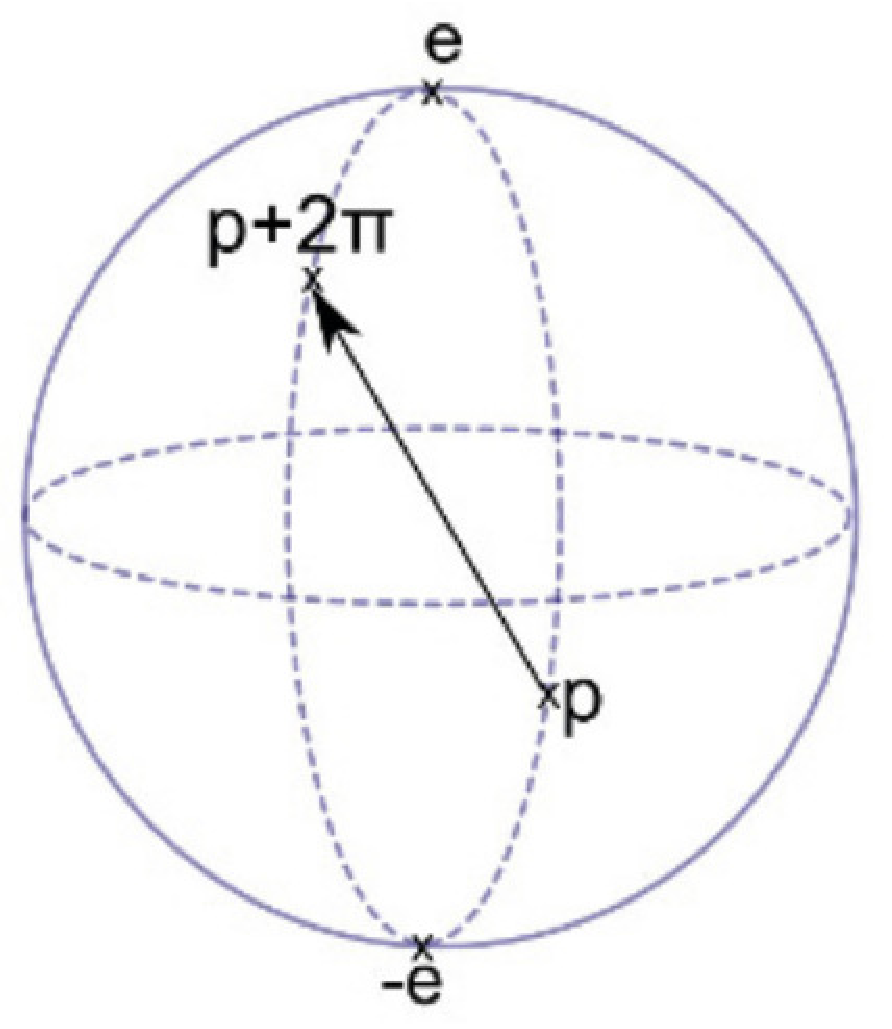
\includegraphics[scale=0.3]{fig3_7.pdf}
		\caption{三维超球面$S^3$的一个二维切面($S^3$自身是四维超球的“表面”,愚蠢的人类没法直接把它画出来),图中可见球面的上半部分对应$\mathcal{SO}(3)$,因为从$\mathcal{SU}(2)$到$\mathcal{SO}(3)$的映射将前者中的$p$点与$p + 2\pi$映射到后者中的同一点。}
	}

因此从流形的角度看,$\mathcal{SU}(2)$群比$\mathcal{SO}(3)$更完整,$\mathcal{SO}(3)$只是其中的一部分。

本书的指导思想之一就是用最基本的群描述大自然最基本的对称性。具体到三维旋转的情况,我们采用$\mathcal{SU}(2)$而非$\mathcal{SO}(3)$。之后其他的对称性我们都这么处理。

世界似乎就是这么设计的!\footnote{先不管设计者有没有、到底是谁吧}比如必须用Poincar\'e群的双覆盖表示来描述基本粒子,而常用却不完整的4-向量表示就不行。要从最深刻的层面描述自然,必须使用覆盖群,而非从覆盖群导出的其他群。

给定一个Lie代数,我们可以通过Lie代数的表示来导出它的覆盖群的表示\mpar{“表示”的具体含义下一节就讲。},然后把Lie代数元素(生成元)的矩阵表示扔进$\mathrm{e}$指数里面就能得到任意群元的矩阵表示。

这就是Lie理论的威力所在。人类通过纯数学就能揭示自然的某些深刻规律。狭义相对论的标准对称群隐藏了一些真相\mpar{学过量子力学的人可能听说过:标准对称群不能告诉我们自旋!},因为它(尽管常用)不是这一对称性对应的最基本的覆盖群。Poincar\'e群\mpar{简明起见,我们省略了“双覆盖”或“覆盖群”的说法,我们利用Poincar\'e群的一个表示导出相应的Lie代数,然后利用此Lie代数导出相应覆盖群的表示,也就是Poincar\'e双覆盖群的表示。}的覆盖群才是最基本的,我们用它描述自然。

总结一下\mpar{$S^2$未出现,没有与$S^2$对应的Lie群,因为没有三维复数。我们从二维复数$i$直接跳到了四维的四元数$\mathbf{i,j,k}$。}:

\begin{itemize}
	\item $S^1 \hat{=} \mathcal{U}(1) \underbrace{\longleftrightarrow}_{\text{一一对应}} \mathcal{SO}(2)$
	\item $S^3 \hat{=} \mathcal{SU}(2) \underbrace{\longrightarrow}_{\text{二对一}} \mathcal{SO}(3) \hat{=} S^3$的一半

		$\Rightarrow \mathcal{SU}(2)$是Lie代数$[J_i, J_j] = i\epsilon_{ijk} J_k$ \, (\eqref{equ3.83}\text{式})的覆盖群,因为$S^3$是单连通流形。
\end{itemize}

下一节介绍Lie理论的重要分支——表示论。表示论使我们能够从任意Lie群导出相应基本群。



\section[表示论]{Representation Theory 表示论}
\label{sec3.5}
群论可以描述变换本身而不必联系现实中的特定对象,这是群论的重要特征。

理论上经常从抽象观点来考虑一个群。这意味着用流形结构与群乘法定义群。例如$\mathcal{SU}(2)$就是$S^3$(超球面),群元就是流形中的点,群乘法规定两个群元$a,b$怎样结合,且满足群公理。搞物理的更关心一个群到底能做什么,即{\itshape 群作用}。

{\bfseries 同一个}群能作用于{\bfseries 许多}不同种类的东西\mpar{这话的含义稍后会更加清楚。},这一重要事实使我们定义了{\bfseries 表示}的概念:群$G$的一个表示就是从$G$到{\itshape 某个向量空间$V$上全体线性变换组成的集合}\mpar{本书中$V$上的线性变换其实就是指矩阵,即表示$R$把群元映射为矩阵,矩阵通过矩阵乘法作用于向量空间中的向量。}的映射,将表示记作$R$, 映射
\begin{equation}
\label{equ3.86}
R: \underbrace{g}_{\in G} \mapsto R(g)
\end{equation}
其中$R(g)$表示$V$上的某个线性变换。映射$R$必须满足如下条件\mpar{满足这些条件的映射称为{\bfseries 同态映射},同构映射当然是同态的,并且比同态性还多了一一映射的特征。}:
\begin{itemize}
	\item $R(e) = I$, 恒等元对应的线性变换是恒等变换。
	\item $R(g^{-1}) = \big( R(g) \big)^{-1}$, 逆元对应的变换是逆变换。
	\item $R(g) \circ R(h) = R(g \circ h)$, 群元$g,h$结合对应的变换等于他们分别对应变换的结合。
\end{itemize}

群的表示\mpar{表示的定义可以进行推广,不一定非得是向量空间(别的空间也行)上的线性变换(非线性也可能),拓展后的映射叫{\bfseries realization}。物理主要考虑向量空间中的线性变换(例如量子力学的Hilbert空间、狭义相对论的Minkowski空间),因此对物理而言表示比更广泛的realization更重要。}将抽象的群元(群流形上的点)与向量空间中的线性变换相联系。尽管按定义来讲,表示是个映射,但大多数情况把表示看做许多矩阵的集合就行了。例如,向量空间\mpar{$\mathbb{R}^3$表示三维Euclidean空间,它的元素就是三维向量,附录A.1里面有很多例子。}$\mathbb{R}^3$中的旋转矩阵组成的集合就是$\mathcal{SO}(3)$群的一个表示,旋转矩阵就是$\mathbb{R}^3$上的线性变换。注意$\mathcal{SO}(3)$群对应的变换也可以作用到其他向量空间。
%不知道`realization'应该怎么翻译

表示论让我们能系统研究同一个群对不同向量空间的作用,这让群论变得精彩多了。

$\mathcal{SU}(2)$是在物理里最常用的群之一。它可以作用到许多向量空间上,比如作用于一维复数向量空间$C^1$,稍后会看到结果是很平凡的。再比如作用于$C^2$,下面我们会详细探究这种作用,$C^2$的元素是二维复数向量,因此$\mathcal{SU}(2)$的群元以$2 \times 2$复数矩阵的形式出现,这是$\mathcal{SU}(2)$最常用的表示,之前一直采用此表示。$\mathcal{SU}(2)$还可作用到$C^3$,前人已经对此有完备的研究,$\mathcal{SU}(2)$作用于$3$维复向量的时候以$3 \times 3$矩阵的形式出现。剧透:$\mathcal{SU}(2)$的$C^3$版本的生成元是\mpar{下一节(\ref{sec3.6.5})就推倒(无误)它,这里只是为了说明就算是$\mathcal{SU}(\text{`}2\text{'})$,也可以作用于三维向量。}:\footnote{原文下式$J_3$的形式有误,译文已按勘误表修改。}
\begin{equation}
\label{equ3.87}
J_1 = \frac{1}{\sqrt{2}}
	\begin{pmatrix}
		0 & 1 & 0 \\
		1 & 0 & 1 \\
		0 & 1 & 0
	\end{pmatrix}
, \quad
J_2 = \frac{1}{\sqrt{2}}
	\begin{pmatrix}
		0 & -i & 0 \\
		i & 0 & -i \\
		0 & i & 0
	\end{pmatrix}
, \quad
J_3 = \frac{1}{\sqrt{2}}
	\begin{pmatrix}
		1 & 0 & 0 \\
		0 & 0 & 0 \\
		0 & 0 & -1
	\end{pmatrix}
\end{equation}

把生成元扔进$\mathrm{e}$指数里就可得到$\mathcal{SU}(2)$的群元在这个表示之下对应的矩阵的形式。

上面的路可以一直走到$C^n$。因此作者纳闷人们为啥叫把这个群叫$\mathcal{SU}(2)$而非$S^3$。\mpar{在作者撰写本书手稿时就把这个群叫$S^3$,考虑到这个非标准名字会对初学者造成困扰所以改了,因为主流教科书都用$\mathcal{SU}(2)$。}但$\mathcal{SU}(2)$通常定义为满足如下条件的$2 \times 2$(是$2$哟!)复数矩阵集合(即\eqref{equ3.33}式)
\begin{equation}
\label{equ3.88}
\mathcal{U}^\dag \mathcal{U} = \mathbf{1}, \quad \det (\mathcal{U}) = 1
\end{equation}
下面会把$\mathcal{SU}(2)$的群元写成$3 \times 3$矩阵的形式,因此要牢记当谈论一般情况$\mathcal{SU}(2)$或其他群群元的时候,我们指的是抽象的群流形中的点,而非只是$2 \times 2$矩阵或者别的。

本章前面都是从群的某个表示出发定义一个群的。比如用$2 \times 2$矩阵定义$\mathcal{SU}(2)$,此方法的优点是群的含义十分具体。在入门之后,把群视为抽象流形的观点\mpar{例如把$\mathcal{SU}(2)$视为$S^3$}更有效,因为这样可以更方便地找出其他有用的群表示。

下面定义几个之后要用的概念,它们与表示的“等级”有关(不是所有表示都是基本的)。


首先是{\bfseries 相似变换}。给定任意矩阵$R$与可逆\mpar{矩阵$S$可逆的含义是存在矩阵$T$使得$ST = TS = \mathbf{1}$,$S$的逆矩阵一般记作$S^{-1}$。}矩阵$S$。则通过可逆矩阵进行相似变换得到:
\begin{equation}
\label{equ3.89}
R \rightarrow R' = S^{-1} RS
\end{equation}

相似变换与表示的关系在于,给定群$G$,群的表示$R(G)$以及任意可逆矩阵$S$,则$S^{-1} RS$也是群表示。这可以从群的定义直接看出来:$\forall g_1, g_2 \in G$,表示$R$把群元映射为向量空间$V$上的线性变换$R(g_1),R(g_2)$。群的定义要求:
\begin{equation}
\label{equ3.90}
R(g_1) R(g_2) = R(g_1 g_2)
\end{equation}
现在把表示进行相似变换:
\begin{equation}
\label{equ3.91}
S^{-1} R(g_1) \underbrace{SS^{-1}}_{=1} R(g_2) S = S^{-1} R(g_1) R(g_2) S = S^{-1} R(g_1 g_2) S
\end{equation}
上式可得$S^{-1} RS$也是一个表示。如果我们有一个表示,那么就能利用任意可逆矩阵变出好多其他表示,新表示的形式可以更漂亮(比如让它是对角矩阵)。

第二个概念:{\bfseries 不变子空间}。给定群$G$在向量空间$V$上的表示$R$, 如果$V' \subset V$满足:
\[
\forall v \in V', g \in G, \text{都有} R(g)v \in V'
\]
则$V'$称为$V$的不变子空间\mpar{自然$v \in V$,子空间$V' \subset V$,换言之$V'$的任意元素都是$V$的元素。}。

任意群元作用于$V'$中的任意向量所得向量仍然在$V'$内,这就可以在$V'$上定义群$G$的表示$R'$了:
\begin{equation}
\label{equ3.92}
R'(g) v = R(g) v,\quad \forall v \in V', g \in G
\end{equation}
这种情况下,表示$R$就有一种不够基本的感觉,它更像是多个小基本部件所构成的。我们称原来的表示$R$不是原来的向量空间$V$的基本表示,$R‘$称为子表示。%flag: but a composite of amaller building blocks 未翻译

定义了上述概念之后就能引入超级重要的{\bfseries 不可约表示}。群$G$在向量空间$V$上的不可约表示$R$意味着除了$0$空间和$V$自身之外再无不变子空间。不可约表示是基本的,它们不能再分解为子表示。利用所有的不可约表示可导出其他所有表示。

还可以从另一个角度看不可约表示:不可约表示不能通过相似变换变成分块对角矩阵形式。而可约表示能被相似变换变成分块对角形式。表示的可约性很关键,比如描述基本粒子要用不可约表示\mpar{要不用啥呢?(译者注:原文为`What else?')},%flag: 边注里的what else没看懂啥意思。。。
基本粒子在变换下的行为由相应对称群的不可约表示描述。

一个群有许多表示\mpar{比如我们前面讨论了二维旋转变换的两种方法——单位复数、$2 \times 2$矩阵。它们都是群流形$S^1$的表示。},怎么知道哪个是描述自然的基本表示?Casimir元可以给我们答案。Casimir元(记作$C$)从Lie代数的元素——生成元导出,它的定义是,对任意生成元$X$都有
\begin{equation}
\label{equ3.93}
[C, X] = 0
\end{equation}
著名的Schur引理\mpar{Schur引理是群论的基本结论之一,它在任何一本群论书都有。}告诉我们,给定一个不可约群表示$R: \mathfrak{g} \rightarrow GL(V)$\footnote{$GL(V)$表示向量空间$V$上所有线性变换组成的集合。},如果某个线性变换$T: V \rightarrow V$(即$T \in GL(V)$)与所有$R(g), \forall g \in G$对易\footnote{即$\forall g \in G, [R(g), T] = 0$。},则$T$必为恒等变换的常数倍。因此Casimir元是群表示的‘常数’,这些‘常数’的值自然地为群表示‘编号’\mpar{具体内容见下一节的例子。}。之后我们就从Casimir元对应编号最低的不可约表示开始。

群表示的定义与向量空间$V$有关。一个表示就是将抽象群到$V$的线性变换的映射。线性代数告诉我们以任意矩阵的本征向量为基可以张成一个向量空间。任意Lie群的生成元至少有一个可以通过相似变成对角矩阵\mpar{对角生成元的集合称为Cartan子代数,相应的集合元素称为Cartan生成元。它们在量子场论中大放异彩,因为Cartan生成元的本征值可以给基本粒子“编号”。例如量子色动力学使用$\mathcal{SU}(3)$群,它有两个Cartan生成元。因此色动力学描述的粒子都有两个“编号”。通常不用数字表示编号,而是用“色”(红、蓝、绿…)来标注。再比如描述弱相互作用的$\mathcal{SU}(2)$群只有一个Cartan生成元,因此每个粒子只有一个标签——Cartan生成元的本征值。},然后这个对角生成元的本征向量就可作为向量空间的基。

下一节导出$\mathcal{SU}(2)$群的不可约表示。研究$\mathcal{SU}(2)$是因为Lorentz群的Lie代数是两份$\mathcal{SU}(2)$的Lie代数。Lorentz群是Poincar\'e群的一部分,本章由浅入深对他们逐一讨论。



%%%%%%%%%%%%%%%%

\section[$\mathcal{SU}$(2)]{$\mathcal{SU}$(2)  特殊幺正群$\mathcal{SU}$(2)}\label{sec3.6}

我们在\ref{sec3.4.3}小节中用具体的矩阵形式进行计算得到了$\mathcal{SU}$(2)生成元的Lie括号\mpar{想当年我们就是用这东西抽象地定义了群的Lie代数。具体结果见
\eqref{equ3.83}式}。通过这一点便能得到$\mathcal{SU}(2)$群的进一步表示。回到开头我们对$\mathcal{SU}(2)$群的表示,即$2\times 2$ 的幺正矩阵,其行列式的值为1,但这只是一个特例罢了。在进一步处理这个问题之前,我们可以想一想大概能得到什么样的表示。

\subsection[$\mathcal{SU}$(2)群的有限维不可约表示]{The Finite-dimensional Irreducible Representations of $\mathcal{SU}$(2) $\mathcal{SU}$(2)群的有限维不可约表示}
\label{sec3.6.1}

为了知道$\mathcal{SU}$(2)群有限维不可约表示的一些东西,我们用在\ref{sec3.4.3}小节中出现的算符的线性组合来定义一个新的算符
\mpar{我们总是能让{\bf{一个}}生成元对角化。遵从惯例,我们选$J_3$为对角阵,由此也生出了矢量空间的基矢。此外,人们一般都是按书上的这种方法引入$J_\pm$的。}:
\begin{align}\label{equ3.94}
  J_+=\frac{1}{\sqrt{2}}(J_1+iJ_2) \\
\label{equ3.95}
  J_-=\frac{1}{\sqrt{2}}(J_1-iJ_2)
\end{align}
用\eqref{equ3.83}式可以验证新定义的算符满足如下对易关系:
%Looks better if equ3.96 and equ3.97 are left aligned
\begin{align}
  &[J_3,J_\pm]=\pm J_\pm \label{equ3.96} \\
  &[J_+,J_-]=J_3. \label{equ3.97}
\end{align}
若$v$为$J_3$本征矢,本征值为$b$\mpar{即$J_3 v=bv$,详见附录\ref{appendix.C.4}。},用新的算符作用在$v$上会得到很有意思的结果:
\begin{eqnarray}\label{equ3.98}
% \nonumber to remove numbering (before each equation)
\nonumber  J_3(J_\pm v) &=& J_3(J_\pm v)+\underbrace{J_\pm J_3 v -J_\pm J_3 v}_{=0} \\
\nonumber               &=& \underbrace{J_\pm J_3 v}_{=J\pm bv} +\underbrace{J_3J_\pm v -J_\pm J_3 v}_{=[J_3,J_\pm]v}\\
                        &\underbrace{=}_{\eqref{equ3.96}\text{式}}& (b\pm 1)J_\pm v
\end{eqnarray}
可见$J_\pm v$也是$J_3$的本征矢,本征值为$(b\pm 1)$,记该本征矢为$w$,则:
\begin{equation}\label{equ3.99}
  J_3 w=(b\pm 1)w \quad \text{以及} \quad w=J_\pm v
\end{equation}

算符$J_-$和$J_+$通常称为降算符和升算符,也称{\bf{阶梯算符(ladder operators)}}。我们可以通过重复利用阶梯算符$J_\pm$来得到关于$J_3$的本征矢,但这个过程不能无休止地进行,因为不同本征值的本征矢之间是线性独立的,而我们处理的是有限维的表示。这意味着相应的矢量空间是有限维的,我们只能得到有限个独立的矢量。

%此处书上的符号比较混乱,译者对此进行了调整
%感觉没有必要调整,给v_{max}加删除线是为什么?
我们推断一定有一本征矢对应着最大的本征值{{$v_{max}$}}。 若把$J_+$作用到$v$上N次以后,得到本征值最大的本征矢$v_{max}$
\begin{equation}\label{equ3.100}
  v_{max}=J_+^N v
\end{equation}
我们有
\begin{equation}\label{equ3.101}
  J_+v_{max}=0
\end{equation}
因为$v_{max}$已经是有最大本征值的本征矢了。称最大本征值为$j:=b+N$。相应有对应着最小本征值的本征矢$v_{min}$,满足
\begin{equation}\label{equ3.102}
  J_-v_{min}=0
\end{equation}
把$J_-$作用到$v_{\color{red}max}$上M次以后,得到本征值最小的本征矢$v_{min}$
\begin{equation}\label{equ3.103}
  v_{min}=J_-^M v_{max}
\end{equation}
因此,$v_{min}$对应的本征值为$j-M$。为进一步讨论,我们需要知道$J_\pm$作用到本征矢上的具体形式。上述的计算说明,$J_- v_k$应等于$v_{k-1}$乘上一常数:
\begin{equation}\label{equ3.104}
  J_- v_k=\alpha_k v_{k-1}
\end{equation}
如果非要深究$J_-$作用到$v_{max}$上的细节的话,那我只能告诉你
\mpar{见Matthew Robinson. Symmetry and the Standard Model. 第90页,Springer, 1st edition, August
2011. ISBN 978-1-4419-8267-4.} $\alpha$满足
\begin{equation}\label{equ3.105}
  \alpha_{j-k}=\frac{1}{\sqrt{2}}\sqrt{(2j-k)(k+1)}
\end{equation}
注意到当$k=2j$时$\alpha$为0,因此,经过$2j$步之后,我们从梯子的顶端到达了底端。$v_{min}$的本征值即是$j-2j=-j$。 总的来说,我们得到了$2j+1$个本征态的本征值
\begin{equation}\label{equ3.106}
  \{-j,-j+1,\dots,j-1,j\}
\end{equation}
此式仅当$j$为整数或半整数\mpar{不信的话你就用分数试试看!}时成立。因为我们有$2j+1$个线性独立的本征矢,故矢量空间应为$2j+1$维
\mpar{见此书 189页: Nadir
Jeevanjee. An Introduction to Tensors and
Group Theory for Physicists. Birkhaeuser,
1st edition, August 2011. ISBN 978-
0817647148}。{\it{这些$J_3$的本征矢构成了完备的矢量空间,因为$J_1$和$J_2$ 能够被$J_+$和$J_-$线性表示,就算是一个任意的线性组合$\sum_i a_i v_i$也能变换成另一种线性组合$\sum_i b_i v_i$,其中$a_i ,b_i$是常数。因此,$J_3$ 的本征矢构成了$V$的一个非平庸不变子空间,而我们也在寻找能构成完备矢量空间$V$的不可约表示}}。

我们可以利用上面定义的$2j+1$维的矢量空间及$J_3$的本征矢$v_k$来给出$\mathcal{SU}$(2)的一个表示。进一步说,我们能证明$\mathcal{SU}$(2)的每一种不可约表示都等价于这一种\mpar{例如此书 190页: Nadir
Jeevanjee. An Introduction to Tensors and
Group Theory for Physicists. Birkhaeuser,
1st edition, August 2011. ISBN 978-
0817647148}。

\subsection[$\mathcal{SU}$(2)的 Casimir算符]{The Casimir Operator of $\mathcal{SU}$(2)  $\mathcal{SU}$(2) 的 Casimir算符}
\label{sec3.6.2}
如第\ref{sec3.5}节所述,我们可以用Casimir算符来标记不同的群表示。$\mathcal{SU}$(2)恰好有一个Casimir算符\mpar{回想一下,Casimir算符指的是那些与群中每个生成元都对易的群元,即$[C,X]=0$。}:
\begin{equation}\label{equ3.107}
  J^2:=(J_1)^2+(J_2)^2+(J_3)^2
\end{equation}
满足定义的条件:
\begin{equation}\label{equ3.108}
  [J^2,J_i]=0
\end{equation}
我们可以用\eqref{equ3.95}式和\eqref{equ3.94}式定义的$J_\pm$ 来重新表示$J^2$:
\begin{eqnarray}
% \nonumber to remove numbering (before each equation)
\nonumber  J^2 &=&J_+J_- + J_-J_+ +(J_3)^2\\
\nonumber      &=& \frac{1}{2}(J_1+iJ_2)(J_1-iJ_2)+\frac{1}{2}(J_1-iJ_2)(J_1+iJ_2)+(J_3)^2   \\
\nonumber      &=& \frac{1}{2}((J_1)^2-iJ_1J_2+iJ_2J_1+(J_2)^2)+\frac{1}{2}((J_1)^2+iJ_1J_2-iJ_2J_1+(J_2)^2)\\
\nonumber      &&+(J_3)^2 \\
\label{equ3.109}
               &=& (J_1)^2+(J_2)^2+(J_3)^2 \quad \checkmark
\end{eqnarray}
带入\mpar{这些东西只是一些归一化常数,如果我们将$J_\pm$作用到归一态上,得到的结果一般都不是归一化的。然而,学物理的都喜欢用归一态,详细的原因以后再谈。这些常数的推导有些无聊,大体思路是先假设c是个归一化常数, 然后从$J_\pm v_k= c v_{k\pm 1}$开始。计算过程能在大多数的量子力学教材中找到(讲角动量和角动量算符那块儿)。如果你不知道也没关系,因为这节讲的对接下来要讲的东西不是太重要。}
\begin{equation}\label{equ3.110}
  J_+v_k=\frac{1}{\sqrt{2}}\sqrt{(j+k+1)(j-k)} v_{k+1}
\end{equation}
以及
\begin{equation}\label{equ3.111}
  J_-v_k=\frac{1}{\sqrt{2}}\sqrt{(j+k)(j-k+1)} v_{k-1}
\end{equation}
我们就能计算对于每个表示都成立的系数\footnote{原文下式有误,译文已按勘误表修改。}:
\begin{eqnarray}
% \nonumber to remove numbering (before each equation)
  \nonumber  J^2 v_k&=&(J_+J_- + J_-J_+ +(J_3)^2)v_k \\
  \nonumber         &=&J_+J_-v_k + J_-J_+v_k +(J_3)^2v_k \\
  \nonumber         &=& J_+ \frac{1}{\sqrt{2}}\sqrt{(j+k)(j-k+1)} v_{k-1}+J_-\frac{1}{\sqrt{2}}\sqrt{(j+k+1)(j-k)} v_{k+1} +k^2v_k  \\
  \nonumber         &=& \frac{1}{\sqrt{2}}\sqrt{(j+k)(j-k+1)} J_+v_{k-1}+\frac{1}{\sqrt{2}}\sqrt{(j+k+1)(j-k)}J_- v_{k+1} +k^2v_k  \\
  \nonumber         &=& \frac{1}{\sqrt{2}}\sqrt{(j+k)(j-k+1)}   \frac{1}{\sqrt{2}}  \sqrt{(j+(k-1)+1)(j-(k-1))}v_{k}   \\
  \nonumber          && +\frac{1}{\sqrt{2}}\sqrt{(j+k+1)(j-k)} \frac{1}{\sqrt{2}} \sqrt{(j+(k+1))(j-(k+1)+1)} v_{k} +k^2v_k  \\
   \nonumber        &=&\frac{1}{2}(j+k)(j-k+1)v_k +\frac{1}{2}(j-k)(j+k+1)v_k+k^2v_k\\
\label{equ3.112}
                    &=&(j^2+j)v_k=j(j+1)v_k
\end{eqnarray}
现在会看这种表示下的几个特例,当然,从最简单的低维数情况开始。

\subsection[$\mathcal{SU}$(2)的一维表示]{The Representation of $\mathcal{SU}$(2) in one Dimension $\mathcal{SU}$(2)的一维表示}
\label{sec3.6.3}
$j$的最小可能值为0,这样群的表示是一$\,2j+1=2 \cdot 0+1=1$ 维矢量空间。可以看出这个表示是平庸的,因为只有$1 \times 1$矩阵满足$\mathcal{SU}$(2)李代数的对易关系$[J_l,J_m]=i\varepsilon_{lmn} J_n=0$。而生成元0的指数映射得到的是变换$\mathcal{U}=e^0=1$,即群的恒等元。

\subsection[$\mathcal{SU}$(2)的二维表示]{The Representation of $\mathcal{SU}$(2) in two Dimension $\mathcal{SU}$(2)的二维表示}
\label{sec3.6.4}
接下来我们讨论$j=\frac{1}{2}$的情况,这个表示是$\,2j+1=2 \cdot \frac{1}{2}+1=2$ 维的。群的生成元$J_3$的本征值为$\frac{1}{2}$和$\frac{1}{2}-1=-\frac{1}{2}$,正如从\eqref{equ3.106} 式中所见,因此$J_3$可表示为
\begin{equation}\label{3.113}
  J_3=\frac{1}{2}\left(
                   \begin{array}{cc}
                     1 & 0 \\
                     0 & -1 \\
                   \end{array}
                 \right)
\end{equation}
此处我们选择$J_3$为对角化的生成元\mpar{由于对易关系, $\mathcal{SU}$(2)群仅有一个对角化的生成元。还有就是记住我们可以用相似变换把一个不对角的生成元变成对角的。}。对应其本征值$+\frac{1}{2}$和$-\frac{1}{2}$的本征矢为:
\begin{equation}\label{equ3.114}
  v_\frac{1}{2}=\left(
                  \begin{array}{c}
                    1 \\
                    0 \\
                  \end{array}
                \right)
                \quad \text{以及} \quad
     v_{-\frac{1}{2}}=\left(
                  \begin{array}{c}
                    0\\
                    1\\
                  \end{array}
                \right)
\end{equation}

可以用在这一基矢下的阶梯算符来得到$\mathcal{SU}$(2)另外两个生成元的矩阵形式
\begin{align}\label{equ3.115}
  J_1=\frac{1}{\sqrt{2}}(J_-+J_+) \\
\label{equ3.116}
  J_2=\frac{i}{\sqrt{2}}(J_--J_+)
\end{align}
这一点可以直接从\eqref{equ3.95}式和\eqref{equ3.94}式关于$J_\pm$的定义的得到。回忆一下,表示空间中的基矢是由$J_3$ 的本征矢给出的,而我们也基矢给出 用$J_1,J_2$。换句话说,$J_1,J_2$是由它们作用在$J_3$ 的本征矢上的效果来定义的。例如
\begin{equation}\label{equ3.117}
  J_1v_\frac{1}{2}
  =\frac{1}{\sqrt{2}}
  (J_-+J_+)v_\frac{1}{2}
  =\frac{1}{\sqrt{2}}
  (J_-v_\frac{1}{2}
  +\underbrace{J_+v_\frac{1}{2}}_{=0})
  =\frac{1}{\sqrt{2}}J_-v_\frac{1}{2}
  =\frac{1}{2}v_{-\frac{1}{2}}
\end{equation}
式中用到$J_+v_\frac{1}{2}=0$,因为$\frac{1}{2}$是最大的本征值。最后结果的系数$\frac{1}{2}$是从\eqref{equ3.105}式得到的。同理可得
\begin{equation}\label{equ3.118}
  J_1 v_{-\frac{1}{2}}=\frac{1}{\sqrt{2}}(J_-+J_+)v_{-\frac{1}{2}}=\frac{1}{2}v_{-\frac{1}{2}}
\end{equation}
而我们之前得到的基矢是$v_\frac{1}{2}=(1,0)^{{T}}$ 和$v_{-\frac{1}{2}}=(0,1)^{{T}}$,因此$J_1$的矩阵为:
\begin{equation}\label{equ3.119}
  J_1=\frac{1}{2}\left(
                   \begin{array}{cc}
                     0 & 1 \\
                     1 & 0 \\
                   \end{array}
                 \right)
\end{equation}
可以验证上式满足我们所说的$J_1$作用到基矢上的效果
\mpar{推导出的\eqref{equ3.117}式为$J_1v_\frac{1}{2}=\frac{1}{2}v_{-\frac{1}{2}}$。带入这里具体的矩阵形式可得
$J_1 v_\frac{1}{2}=\frac{1}{2}
\left(
\begin{array}{cc}
0 & 1 \\
1 & 0 \\
\end{array}
\right)
\left(
\begin{array}{c}
      1 \\
      0 \\
\end{array}
\right)
=\frac{1}{2}
\left(
\begin{array}{c}
      0 \\
      1\\
\end{array}
\right)=\frac{1}{2}v_{-\frac{1}{2}} \quad \surd$。}。 同理可得
\begin{equation}\label{equ3.120}
    J_2=\frac{1}{2}\left(
                   \begin{array}{cc}
                     0 & -i \\
                     i & 0 \\
                   \end{array}
                 \right)
\end{equation}
正如我们在这一章开头寻找$\mathcal{SU}(2)$群Lie代数时所发现的一样(\eqref{equ3.81}式),这些生成元$J_i=\frac{1}{2}\sigma_i$正是Pauli 矩阵。可以看出,现在使用表示的是二维表示。当然除此之外还有其他的表示形式,例如我们下节会看到的三维空间中的表示\mpar{再次说明,$\mathcal{SU}(2)$最开始的定义是全体行列式值为1的$2\times 2$幺正矩阵的集合,而在这儿我们采用抽象的定义,即其对应的流形$S^3$,接下来还要讨论这个群的更高维表示,比如$3\times 3$ 矩阵的表示。其实叫成别的名字可能更合适(比如说对应的流形$S^3$),但按照传统,它就叫$\mathcal{SU}(2)$.}。
\subsection[$\mathcal{SU}$(2)的三维表示]{The Representation of $\mathcal{SU}$(2) in two Dimension $\mathcal{SU}$(2)的三维表示}
\label{sec3.6.5}
重复与二维情况相似的操作\mpar{仍然是从对角化的生成元$J_3$出发。$J_3$的本征值为(1,0,-1),因此立刻就能得到其矩阵形式。对于$J_1,J_2$而言,仍然是从其作用结果出发,即把他们写成$J_\pm$的线性组合然后作用到$J_3$的本征矢上。} 可以得到\footnote{原文下式$J_3$的形式有误,译文已按勘误表修改。}:
\begin{equation}\label{equ3.121}
J_1=\frac{1}{\sqrt{2}}\left(
\begin{array}{ccc}
0& 1 & 0 \\
1 & 0 & 1 \\
0 & 1 & 0 \\
  \end{array}
\right)
J_2=\frac{1}{\sqrt{2}}\left(
\begin{array}{ccc}
0& -i & 0 \\
i & 0 & -i \\
0 & i & 0 \\
\end{array}
\right)
J_3=\frac{1}{\sqrt{2}}\left(
\begin{array}{ccc}
1 & 0 & 0 \\
0 & 0 & 0 \\
0 & 0 & -1 \\
\end{array}
\right)
\end{equation}
这就是$\mathcal{SU}(2)$的三维表示。如果你有兴趣的话,还可以推出三维表示下$\mathcal{SU}(2)$群元的形式(把生成元扔进$\mathrm{e}$指数里)。介于现在所学已足够理解最重要的Lorentz 群的表示,我们将不会推导更高维的$\mathcal{SU}(2)$表示。
%%%%%%%%%%%%%%%



\section[Lorentz群]{The Lorentz Group $\mathcal{O}(1, 3)$ \quad Lorentz群$\mathcal{O}(1, 3)$}
\label{sec3.7}

\begin{quote}
抽象总是从具体的现实中产生的$\dots$ 你总得从某件事物出发,最后才能把所有现实的痕迹抹除掉。
\end{quote}

\begin{flushright}
{\bfseries  --- Pablo Picasso}\mpar{引自 Robert S. Root-Bernstein and Michele M. Root-Bernstein. Sparks of Genius. Mariner Books, 1st edition, 8\, 2001. ISBN 9780618127450}
\end{flushright}

本节从Lorentz群{\bfseries 一种}常用的表示出发导出相应的Lie代数。推导过程与之前$\mathcal{SU}(2)$的情形相同——用$\mathcal{SU}(2)$的$2 \times 2$矩阵表示导出了Lie代数。我们会发现Lorentz群的Lie代数可以用两份$\mathcal{SU}(2)$\ Lie代数表示,这会导出Lorentz群的更多表示。著名的向量表示——即Lorentz群群元为$4 \times 4$矩阵,作用于$4$维向量——仅仅是众多表示中的{\bfseries 一种}。新表示能描述向量表示不能描述的物理系统。这就是Lie理论的威力所在,它使我们找出对称性隐藏的抽象结构,从而可以描述自然最基本的层面。

首先导出Lorentz群及其子群的特性。Lorentz群定义为Minkowski空间中{\itshape 所有保证内积不变的变换}组成的集合\mpar{下式的推导在第2章。重复一下,Lorentz群的定义借鉴了Euclidean空间中旋转、反射变换保证Euclidean空间中内积不变的特性。}:
\begin{equation}
\label{equ3.122}
x^\mu x_\mu = x^\mu \eta_{\mu \nu} x^\nu = (x^0)^2 - (x^1)^2 - (x^2)^2 - (x^3)^2
\end{equation}
其中$\eta_{\mu \nu}$表示Minkowski度规:
\begin{equation}
\label{equ3.123}
\eta_{\mu \nu} =
	\begin{pmatrix}
		1 & 0 & 0 & 0 \\
		0 & -1 & 0 & 0 \\
		0 & 0 & -1 & 0 \\
		0 & 0 & 0 & -1
	\end{pmatrix}
\end{equation}

这也就是我们把Lorentz群叫做$\mathcal{O}(1, 3)$的原因,类似地,群$\mathcal{O}(4)$就是保持内积$ (x^0)^2 + (x^1)^2 + (x^2)^2 + (x^3)^2$的群。这个定义的条件对变换(矩阵)有什么限制?Lorentz群的群元——Lorentz变换通常记作$\Lambda$,考虑变换$x^\mu \rightarrow x'^\mu = \Lambda^\mu_\nu x^\nu$,变换前后的内积为:
\begin{equation}
\label{equ3.124}
x^\mu \eta_{\mu \nu} x^\nu \rightarrow x'^\sigma \eta_{\sigma \rho} x'^\rho = (x^\mu \Lambda^\sigma_\mu) \eta_{\sigma \rho} (\Lambda^\rho_\nu x^\nu) \stackrel{!}{=} x^\mu \eta_{\mu \nu} x^\nu
\end{equation}
由$x^{\mu}$的任意性可得:
\begin{equation}
\label{equ3.125}
\Lambda^\sigma_\mu \eta_{\sigma \rho} \Lambda^\rho_\nu \stackrel{!}{=} \eta_{\mu \nu}
\end{equation}
上式写成矩阵形式\mpar{复习:两个向量的内积用矩阵乘法表示是,左侧的向量转置成行矩阵。因此下式左侧有$\Lambda^T$。}:
\begin{equation}
\label{equ3.126}
\Lambda^T \eta \Lambda \stackrel{!}{=} \eta
\end{equation}
{\bfseries 上式就是Lorentz变换$\Lambda$定义的数学形式!} 对上式取行列式,利用$\det(AB) = \det(A) \det(B)$可得:
\begin{align}
\label{equ3.127}
\det(\Lambda) \underbrace{\det(\eta)}_{= -1} \det(\Lambda) = \underbrace{\det(\eta)}_{= -1} \rightarrow \det(\Lambda)^2 \stackrel{!}{=} 1 \\
\label{equ3.128}
\rightarrow \det(\Lambda) \stackrel{!}{=} \pm 1
\end{align}

取\eqref{equ3.125}式的$\mu = \nu = 0$分量\mpar{稍后就会看到这有什么用。}:
\begin{align}
	\Lambda_0^\sigma \eta_{\sigma \rho} \Lambda_0^\rho \stackrel{!}{=} \underbrace{\eta_{00}}_{=1} \nonumber \\
	\label{equ3.129}
	\rightarrow \Lambda_0^\sigma \eta_{\sigma \rho} \Lambda_0^\rho = (\Lambda_0^0)^2 - \sum_i (\Lambda_0^i)^2 \stackrel{!}{=} 1
\end{align}
由此可得:
\begin{equation}
	\label{equ3.130}
	\Lambda_0^0 \stackrel{!}{=} \pm \sqrt{1 + \sum_i (\Lambda_0^i)^2}
\end{equation}

根据\eqref{equ3.128}与\eqref{equ3.130}式的正负可以把Lorentz群分成4分支。保证坐标系取向\mpar{这意味着右手坐标系在变换后仍为右手系,左手坐标系在变换后仍为左手系。左手、右手坐标系的定义见附录\ref{appendix.A.5}}不变的两个分支满足$\det (\Lambda) = +1$. 如果想保证时间轴的方向不变,则需要条件$\Lambda_0^0 \geq 0$,因为
\begin{equation}
	\label{equ3.131}
	x^0 = t \rightarrow x'^0 = t' = \Lambda_\nu^0 x^\nu = \Lambda_0^0 t + \Lambda_1^0 x^1 + \Lambda_2^0 x^2 + \Lambda_3^0 x^3
\end{equation}
如果$\Lambda_0^0 \geq 0$, 则$t'$与$t$同号。

满足$\det(\Lambda) \geq 0$与$\Lambda_0^0 \geq 0$的分支称为$\mathcal{SO}(1, 3)^{\uparrow}$。我们主要研究这个子群,它的名字很漂亮——正规\mpar{‘正规’(proper)意思是$\mathcal{SO}(1, 3)^{\uparrow}$子群的群元都是保证坐标系取向和宇称不变的变换。}或正时\mpar{‘正时’(orthochronous)是指子群的群元保持时间轴的方向不变。}Lorentz群。Lorentz群的这四分支是分离的,因为从一个分支出发,仅用该分支的Lorentz变换无法得到其他任何分支的元素。但引入两个新变换之后就可以从$\mathcal{SO}(1, 3)^\uparrow$出发得到其他分支\mpar{在现在的群表示下这两个算符的矩阵长这样。后面换用不同的表示,它们会大不一样。}:
\begin{align}
	\label{equ3.132}
	\Lambda_P =
		\begin{pmatrix}
			1 & 0 & 0 & 0 \\
			0 & -1 & 0 & 0 \\
			0 & 0 & -1 & 0 \\
			0 & 0 & 0 & -1
		\end{pmatrix}
\\
	\label{equ3.133}
	\Lambda_T =
		\begin{pmatrix}
			-1 & 0 & 0 & 0 \\
			0 & 1 & 0 & 0 \\
			0 & 0 & 1 & 0 \\
			0 & 0 & 0 & 1
		\end{pmatrix}
\end{align}
$\Lambda_P$称为宇称算符,相应的宇称变换其实就是镜面反射。$\Lambda_T$称为时间反演算符。

于是完整的Lorentz群$\mathcal{O}(1, 3)$可以表示为如下集合:
\begin{equation}
	\label{equ3.134}
	\mathcal{O}(1, 3) = \{ \mathcal{SO}(1, 3)^\uparrow, \Lambda_P \mathcal{SO}(1, 3)^\uparrow, \Lambda_T \mathcal{SO}(1, 3)^\uparrow, \Lambda_P \Lambda_T \mathcal{SO}(1, 3)^\uparrow \}
\end{equation}

这样,研究Lorentz群的表示就可简化为研究$\mathcal{SO}(1, 3)^\uparrow$的表示,因为只要再找出$\Lambda_P$、$\Lambda_T$的表示,Lorentz群的其他分支就都有啦。

\subsection[Lorentz群的$1$表示]{One Representation of the Lorentz Group \quad Lorentz群的$1$表示}
\label{sec3.7.1}
下面利用Lorentz群的定义(\eqref{equ3.125}式)构造Lorentz变换的显式矩阵表示。首先考虑矩阵的形式。对Lorentz群,它的群元作用于$4$向量\mpar{通常狭义相对论涉及的向量空间是四维实Minkowski空间$R^{(1, 3)}$。Lorentz群就是定义在这个空间的(Lorentz变换就是保证$4 \times 4$度规不变的变换),因此首先研究群在$R^{(1, 3)}$上的表示。 类似地,$\mathcal{SU}(2)$群起初是用$2 \times 2$复数矩阵表示的,从那里出发可以得到$\mathcal{SU}(2)$好多其他的表示。},因此群元的形式为$4 \times 4$实数矩阵。矩阵元必须是实数,因为Minkowski空间$R^{(1, 3)}$是实数空间。一般的$4 \times 4$实数矩阵有$16$个参数,而Lorentz群的定义规定了$10$个条件\mpar{自行验证$\Lambda^T \eta \Lambda = \eta$对$\Lambda$的限制条件是$10$个。},这样还剩$6$个自由参数。也就是说描述最一般的Lorentz变换需要$6$个参数。因此只要集齐$6$个线性无关的生成元,就可以召唤Lorentz群的Lie代数。这$6$个生成元构成Lie代数的一组基,即任意生成元可唯一地表示为它们的线性组合。然后就能计算这些基在Lie括号下的运算结果,从而导出Lie代数的抽象定义。

注意三维Euclidean空间中的旋转矩阵(它们只变换空间坐标而不管时间)满足定义\eqref{equ3.125}式。这是因为Minkowski度规的空间部分\mpar{空间部分是指分量$\mu = 1, 2, 3$对应的部分。空间部分通常记作$\eta_{ij}$, 人们习惯用拉丁字母(例如$i,j$)表示从$1$到$3$, 而希腊字母(例如$\mu,\nu$)表示从$0$到$3$。}与$3 \times 3$单位矩阵成比例\mpar{$\eta_{11} = \eta_{22} = \eta_{33} = -1, \eta_{ij}=0, \text{若}i \neq j$}。因此对于只涉及空间坐标的变换,由\eqref{equ3.125}可得:
\begin{align*}
	-R^T I_{3 \times 3} R = - R^T R \stackrel{!}{=} -I_{3 \times 3} \\
	\rightarrow R^T I_{3 \times 3} R = R^T R \stackrel{!}{=} I_{3 \times 3}
\end{align*}
上式正是$\mathcal{O}(3)$群的定义式。再加上条件
\begin{equation*}
	\det(\Lambda) \stackrel{!}{=} 1
\end{equation*}
就是$\mathcal{SO}(3)$群的定义。只涉及空间坐标的Lorentz变换的形式为:
\begin{equation*}
	\Lambda_{\mathrm{rot}} =
		\begin{pmatrix}
			1 & \\
			  & R_{3 \times 3}
		\end{pmatrix}
\end{equation*}
其中旋转矩阵$R_{3 \times 3}$的形式见\eqref{equ3.23}式,相关推导见\ref{sec3.4.1}节。相应的生成元的推导与\ref{sec3.4.1}节相似,结果为:
\begin{equation}
	\label{equ3.135}
	J_i =
		\begin{pmatrix}
			0 & \\
			  & J_i^{3\mathrm{dim}}
		\end{pmatrix}
	,\quad
	i = 1, 2, 3.
\end{equation}
比如,由\eqref{equ3.65}式可得:
\begin{equation}
	\label{equ3.136}
	J_1 =
		\begin{pmatrix}
			0 & \\
			  & J_1^{3 \mathrm{dim}}
		\end{pmatrix}
	=
		\begin{pmatrix}
			0 & 0 & 0 & 0 \\
			0 & 0 & 0 & 0 \\
			0 & 0 & 0 & -1 \\
			0 & 0 & 1 & 0
		\end{pmatrix}
\end{equation}

下面包含时空坐标的变换。按Lie理论的套路,考虑无穷小变换\mpar{Kronecker $\delta$符号定义为
\[\delta^\mu_\rho =
\begin{cases}
	1, & \mu = \rho \\
	0, & \mu \neq \rho
\end{cases}
\]
将Kronecker $\delta$符号写成矩阵形式就是恒等矩阵$I$.
}:
\begin{equation}
\label{equ3.137}
\Lambda^\mu_\rho \approx \delta^\mu_\rho + \epsilon K^\mu_\rho
\end{equation}
将上式带入$\Lambda$的定义条件\eqref{equ3.125}式:
\begin{align}
	\Lambda^\mu_\rho \eta_{\mu \nu} \Lambda^\nu_\sigma \stackrel{!}{=} \eta_{\rho \sigma} \nonumber \\
	\rightarrow (\delta^\mu_\rho + \epsilon K^\mu_\rho) \eta_{\mu \nu} (\delta^\nu_\sigma + \epsilon K^\nu_\sigma) \stackrel{!}{=} \eta_{\rho \sigma} \nonumber \\
	\rightarrow \cancel{\eta_{\rho \sigma}} + \epsilon K^\mu_\rho \eta_{\mu \sigma} + \epsilon K^\nu_\sigma \eta_{\rho \nu} + \underbrace{\epsilon^2 K^\mu_\rho \eta_{\mu \nu} K^\nu_\sigma}_{\text{略去高阶小量} \epsilon^2 \text{项}} = \cancel{\eta_{\rho \sigma}} \nonumber \\
	\rightarrow K^\mu_\rho \eta_{\mu \sigma} + K^\nu_\sigma \eta_{\rho \nu} = 0
\end{align}
写成矩阵形式\mpar{第一个下标表示行指标,第二个是列指标。不过指标为一上一下的时候会混淆,这时我们把上下标错开表示,比如$K^\mu_\rho \equiv K^\mu_{\ \rho} \rightarrow (K^T)^\mu_{\  \rho} = K_\rho^{\ \mu}$。矩阵乘法的定义是用行乘以列,因此$K^\nu_{\ \sigma} \eta_{\rho \nu} = \eta_{\rho \nu} K^\nu_{\ \sigma}$的含义为,矩阵$\eta$的第$\rho$行乘以$K$的第$\sigma$列,用矩阵表示为$\eta K$。此外,$K^\mu_\rho \eta_{\mu \sigma} = K^\mu_{\ \rho} \eta_{\mu \sigma} = (K^T)_\rho^{\ \mu} \eta_{\mu \sigma}$,为将上式表示为矩阵乘法而引入矩阵$K$的转置,只有这样才能表示为行乘以列的形式:$K^T$的第$\rho$行乘以$\eta$的第$\sigma$列,上式用矩阵表示为$K^T \eta$。用指标记号可以自由移项,比如$K^\mu_\rho$只是矩阵$K$得一个元素,即一个数。 }:
\begin{equation}
	\label{equ3.139}
	K^T \eta = -\eta K
\end{equation}

上面导出了时空变换的生成元$K$需满足的条件。这些生成元生成的变换称为{\bfseries 推动}。推动的意思是变换到相对于初始坐标系作匀速直线运动的另一坐标系。比如从一个相对于观者静止的坐标系变换到相对于观者匀速直线运动的坐标系。下面考虑\ref{sec2.1}节中的例子:沿$x$轴的推动变换。由于$y' = y, z' = z$,故生成元的形式为:
\begin{equation}
	\label{equ3.140}
	K_x =
		\begin{pmatrix}
			\underbrace{
				\begin{pmatrix}
					a & b \\
					c & d
				\end{pmatrix}
			}_{\equiv k_x}
			& \\
			&	\begin{pmatrix}
					0 & 0 \\
					0 & 0
				\end{pmatrix}
		\end{pmatrix}
\end{equation}

只需要考虑非零的$2 \times 2$矩阵部分就行了,\eqref{equ3.139}式简化为:
\[
	\begin{pmatrix}
		a & c \\
		b & d
	\end{pmatrix}
	\begin{pmatrix}
		-1 & 0 \\
		0 & 1
	\end{pmatrix}
	= -
	\begin{pmatrix}
		-1 & 0 \\
		0 & 1
	\end{pmatrix}
	\begin{pmatrix}
		a & b \\
		c & d
	\end{pmatrix}
\]
不难解得\mpar{$\begin{pmatrix}0 & 1 \\ 1 & 0 \end{pmatrix} \begin{pmatrix}-1 & 0 \\ 0 & 1 \end{pmatrix} = \begin{pmatrix} 0 & 1 \\ -1 & 0 \end{pmatrix}$,以及\\ $- \begin{pmatrix} -1 & 0 \\ 0 & 1 \end{pmatrix} \begin{pmatrix} 0 & 1 \\ 1 & 0 \end{pmatrix} = -\begin{pmatrix} 0 & -1 \\ 1 & 0 \end{pmatrix}$.}:
\[
	k_x =
		\begin{pmatrix}
			a & b \\
			c & d
		\end{pmatrix}
	=
		\begin{pmatrix}
			0 & 1 \\
			1 & 0
		\end{pmatrix}
\]

因此沿$x$轴的推动变换的生成元为:
\begin{equation}
\label{equ3.141}
	K_x =
		\begin{pmatrix}
			0 & 1 & 0 & 0 \\
			1 & 0 & 0 & 0 \\
			0 & 0 & 0 & 0 \\
			0 & 0 & 0 & 0
		\end{pmatrix}
\end{equation}

同理可以求出沿$y$、$z$轴推动变换的生成元:
\begin{equation}
\label{equ3.142}
	K_y =
		\begin{pmatrix}
			0 & 0 & 1 & 0 \\
			0 & 0 & 0 & 0 \\
			1 & 0 & 0 & 0 \\
			0 & 0 & 0 & 0
		\end{pmatrix}
	, \quad
	K_z =
		\begin{pmatrix}
			0 & 0 & 0 & 1 \\
			0 & 0 & 0 & 0 \\
			0 & 0 & 0 & 0 \\
			1 & 0 & 0 & 0
		\end{pmatrix}
\end{equation}
根据Lie理论,把生成元扔进$\mathrm{e}$指数里就能得到有限大小的变换\mpar{生成元$K_x, K_y, K_z$都是厄米的,即$K_i^\dag = K_i$。因此$\mathrm{e}$指数里不加虚数单位$i$,因为加了之后就变成反厄米的了。}:
\[
	\Lambda_x(\phi) = \mathrm{e}^{\phi K_x}
\]
还以$K_x$为例,简明起见,只考虑其中exciting的部分——$2 \times 2$矩阵$k_x$(见\eqref{equ3.140}式)。将它的指数函数用级数展开式计算,并利用\mpar{不难算出$k_x^2 = \begin{pmatrix} 0 & 1 \\ 1 & 0 \end{pmatrix} \begin{pmatrix} 0 & 1 \\ 1 & 0 \end{pmatrix} = \begin{pmatrix} 1 & 0 \\ 0 & 1 \end{pmatrix}$,然后$k_x^4 = \mathbf{1}$等等等等。对于奇次幂有$k_x^3 = k_x, k_x^5 = k_x, \dots$}$k_x^2 = \mathbf{1}$:
\begin{align}
	\Lambda_x(\phi) &= \mathrm{e}^{\phi k_x} = \sum_{n = 0}^{\infty} \frac{\phi^n k_x^n}{n!} = \sum_{n = 0}^{\infty} \frac{\phi^{2n}}{(2n)!} \underbrace{k_x^{2n}}_{=1} + \sum_{n = 0}^{\infty} \frac{\phi^{2n + 1}}{(2n + 1)!} \underbrace{k_x^{2n + 1}}_{=k_x} \nonumber \\
	&= \left( \sum_{n = 0}^{\infty} \frac{\phi^{2n}}{(2n)!} \right) I + \left( \sum_{n = 0}^{\infty} \frac{\phi^{2n + 1}}{(2n + 1)!} \right) k_x \nonumber \\
	&= \cosh(\phi) I + \sinh(\phi) k_x \nonumber \\
	\label{equ3.143}
	&=
		\begin{pmatrix}
			\cosh(\phi) & 0 \\
			0 & \cosh(\phi)
		\end{pmatrix}
	+
		\begin{pmatrix}
			0 & \sinh(\phi) \\
			\sinh(\phi) & 0
		\end{pmatrix} \nonumber \\
	&=
		\begin{pmatrix}
			\cosh(\phi) & \sinh(\phi) \\
			\sinh(\phi) & \cosh(\phi)
		\end{pmatrix}
\end{align}
计算过程与第\ref{sec3.4.1}节的内容相似。这里的求和式里没出现$(-1)^n$,因此结果不是$\sin(\phi)$和$\cos (\phi)$,而是双曲正弦$\sinh(\phi)$和双曲余弦$\cosh(\phi)$。沿$x$轴推动变换的完整$4 \times 4$矩阵为:
\begin{equation}
\label{equ3.144}
	\Lambda_x =
		\begin{pmatrix}
			\cosh(\phi) & \sinh(\phi) & 0 & 0 \\
			\sinh(\phi) & \cosh(\phi) & 0 & 0 \\
			0 & 0 & 1 & 0 \\
			0 & 0 & 0 & 1
		\end{pmatrix}
\end{equation}
同理可导出沿$y, z$轴的推动变换矩阵:
\begin{align}
\label{equ3.145}
	\Lambda_y =
		\begin{pmatrix}
			\cosh(\phi) & 0 & \sinh(\phi) & 0 \\
			0 & 1 & 0 & 0 \\
			\sinh(\phi) & 0 & \cosh(\phi) & 0 \\
			0 & 0 & 0 & 1
		\end{pmatrix}
	, \\
\label{equ3.146}
	\Lambda_z =
		\begin{pmatrix}
			\cosh(\phi) & 0 & 0 & \sinh(\phi) \\
			0 & 1 & 0 & 0 \\
			0 & 0 & 1 & 0 \\
			\sinh(\phi) & 0 & 0 & \cosh(\phi)
		\end{pmatrix}
\end{align}
任意的推动变换都可以分解为上述三个变换矩阵的乘积。

\subsection[Lorentz群其他部分的生成元]{Generators of the Other Components of the Lorentz Group \quad Lorentz群其他部分的生成元}
\label{sec3.7.2}
为得到Lorentz群其他部分\mpar{复习:Lorentz群可以分成$\mathcal{O}(1, 3) = \{ \mathcal{SO}(1, 3)^\uparrow, \Lambda_P \mathcal{SO}(1, 3)^\uparrow, $
$\Lambda_T \mathcal{SO}(1, 3)^\uparrow, \Lambda_P \Lambda_T \mathcal{SO}(1, 3)^\uparrow \}$,上一节导出了$\mathcal{SO}(1, 3)^\uparrow$的生成元。}生成元的形式,只需将宇称算符$\Lambda_P$和时间反演算符$\Lambda_T$作用于刚刚导出的生成元$J_i, K_i$上,用矩阵指标记法写为\mpar{对$J, K$变换需要两个$\Lambda_P$, 因为$J, K$都是二维矩阵,一维一个$\Lambda_P$。这就是算符矩阵在坐标变换下的一般形式,喵。}:
\begin{align}
\label{equ3.147}
	(\Lambda_P)_{\alpha'}^\alpha (\Lambda_P)_{\beta'}^\beta (J_i)^{\alpha' \beta'}\ \ \  \mathclap{ \underbrace{\hat{=}}_{\text{变成矩阵形式}} }\ \ \  \Lambda_P J_i (\Lambda_P)^T = J_i \hat{=} (J_i)^{\alpha \beta} \\
\label{equ3.148}
	(\Lambda_P)_{\alpha'}^\alpha (\Lambda_P)_{\beta'}^\beta (K_i)^{\alpha' \beta'}\ \ \ \mathclap{ \underbrace{\hat{=}}_{\text{变成矩阵形式}} } \ \ \ \Lambda_P K_i (\Lambda_P)^T = -K_i \hat{=} -(K_i)^{\alpha \beta}
\end{align}
上两式可以用上节导出的$J, K$显式矩阵形式暴力计算,例如\footnote{原文\eqref{equ3.149}, \eqref{equ3.150}式有误,译文已按勘误表修改。}:
\begin{align}
\label{equ3.149}
	J_x &=
		\begin{pmatrix}
			0 & 0 & 0 & 0 \\
			0 & 0 & 0 & 0 \\
			0 & 0 & 0 & -1 \\
			0 & 0 & 1 & 0
		\end{pmatrix}
	\rightarrow
	J_x' = \Lambda_P J_x (\Lambda_P)^T = J_x
\end{align}
因为
\begin{align}
	\Lambda_P J_x (\Lambda_P)^T &=
		\begin{pmatrix}
			1 & 0 & 0 & 0 \\
			0 & -1 & 0 & 0 \\
			0 & 0 & -1 & 0 \\
			0 & 0 & 0 & -1
		\end{pmatrix}
		\begin{pmatrix}
			0 & 0 & 0 & 0 \\
			0 & 0 & 0 & 0 \\
			0 & 0 & 0 & -1 \\
			0 & 0 & 1 & 0
		\end{pmatrix}
		{
		\begin{pmatrix}
			1 & 0 & 0 & 0 \\
			0 & -1 & 0 & 0 \\
			0 & 0 & -1 & 0 \\
			0 & 0 & 0 & -1
		\end{pmatrix}
		}^T
	\nonumber \\
\label{equ3.150}
	&=
		\begin{pmatrix}
			0 & 0 & 0 & 0 \\
			0 & 0 & 0 & 0 \\
			0 & 0 & 0 & -1 \\
			0 & 0 & 1 & 0
		\end{pmatrix}
\end{align}
同理,
\begin{align}
\label{equ3.151}
	K_x &=
		\begin{pmatrix}
			0 & 1 & 0 & 0 \\
			1 & 0 & 0 & 0 \\
			0 & 0 & 0 & 0 \\
			0 & 0 & 0 & 0
		\end{pmatrix}
	\rightarrow K'_x = \Lambda_P K_x (\Lambda_P)^T = -K_x
\end{align}
因为
\begin{align}
	\Lambda_P K_x (\Lambda_P)^T &=
		\begin{pmatrix}
			1 & 0 & 0 & 0 \\
			0 & -1 & 0 & 0 \\
			0 & 0 & -1 & 0 \\
			0 & 0 & 0 & -1
		\end{pmatrix}
		\begin{pmatrix}
			0 & 1 & 0 & 0 \\
			1 & 0 & 0 & 0 \\
			0 & 0 & 0 & 0 \\
			0 & 0 & 0 & 0
		\end{pmatrix}
		{
		\begin{pmatrix}
			1 & 0 & 0 & 0 \\
			0 & -1 & 0 & 0 \\
			0 & 0 & -1 & 0 \\
			0 & 0 & 0 & -1
		\end{pmatrix}
		}^T
\nonumber \\
\label{equ3.152}
	&= -
		\begin{pmatrix}
			0 & 1 & 0 & 0 \\
			1 & 0 & 0 & 0 \\
			0 & 0 & 0 & 0 \\
			0 & 0 & 0 & 0
		\end{pmatrix}
\end{align}

综上,在宇称变换下:
\begin{equation}
\label{equ3.153}
	J_i \underbrace{\longrightarrow}_{\Lambda_P} J_i, \quad K_i \underbrace{\longrightarrow}_{\Lambda_P} -K_i
\end{equation}
它们之后很有用,因为宇称算符在其他表示之下的形式不会像现在的向量表示这样显然。时间反演算符$\Lambda_T$的推导过程相似,由于$\Lambda_T$只变换第一个分量(时间分量),因此只对$K_i$有影响:
\begin{align}
\label{equ3.154}
	(\Lambda_T)_{\alpha'}^\alpha (\Lambda_T)_{\beta'}^\beta (J_i)^{\alpha' \beta'} \ \ \ \mathclap{ \underbrace{\hat{=}}_{\text{变成矩阵形式}} } \ \ \  \Lambda_T J_i (\Lambda_T)^T = J_i \hat{=} (J_i)^{\alpha \beta} \\
\label{equ3.155}
	(\Lambda_T)_{\alpha'}^\alpha (\Lambda_T)_{\beta'}^\beta (K_i)^{\alpha' \beta'} \ \ \ \mathclap{ \underbrace{\hat{=}}_{\text{变成矩阵形式}} } \ \ \ \Lambda_T K_i (\Lambda_T)^T = -K_i \hat{=} -(K_i)^{\alpha \beta}
\end{align}
或者简写为:
\begin{equation}
\label{equ3.156}
	J_i \underbrace{\rightarrow}_{\Lambda_T} J_i, \quad K_i \underbrace{\rightarrow}_{\Lambda_T} -K_i
\end{equation}

\subsection[$\mathcal{SO}(1, 3)^\uparrow$群的Lie代数]{The Lie Algebra of the Proper Orthochronous Lorentz Group \quad $\mathcal{O}(1, 3)^\uparrow$群的Lie代数}
\label{equ3.7.3}
%此处$\mathcal{O}(1, 3)^\uparrow$有误?
利用上节导出的$\mathcal{SO}(1, 3)^\uparrow$生成元的矩阵形式\mpar{推动变换的生成元见\eqref{equ3.141}式,旋转变换的生成元见\eqref{equ3.62}式。}可以直接计算相应的Lie代数\mpar{Levi-Civita符号$\epsilon_{ijk}$的定义见附录\ref{appendix.B.5.5}}:
\begin{align}
\label{equ3.157}
	[J_i, J_j] &= i \epsilon_{ijk} J_k \\
\label{equ3.158}
	[J_i, K_j] &= i \epsilon_{ijk} K_k \\
\label{equ3.159}
	[K_i, K_j] &= -i \epsilon_{ijk} J_k
\end{align}
其中$J_i$是旋转变换的生成元,$K_i$是推动的生成元。一般形式的Lorentz变换可以表示为:
\begin{equation}
\label{equ3.160}
	\Lambda = \mathrm{e}^{i J \theta + i K \Phi}
\end{equation}
\eqref{equ3.158}式表明两种生成元($J_i$与$K_i$)之间不对易。旋转生成元在对易运算下封闭\mpar{在对易运算下封闭意味着对易子$[J_i, J_j] = J_i J_j - J_j J_i$还是一个旋转变换的生成元。\eqref{equ3.157}体现了这一点。},而推动生成元则不是这样\mpar{\eqref{equ3.159}表明两个推动生成元$K_i, K_j$的对易子并非推动生成元,而是个转动生成元。}。从$J_i, K_i$出发可以定义在对易运算下封闭并且相互对易的新生成元\footnote{注意区分之后式子中的虚数单位$i$与指标$i$,我们对作者采用这样的符号很抱歉。}:
\begin{equation}
\label{equ3.161}
	N_i^\pm \equiv \frac{1}{2} (J_i \pm i K_i)
\end{equation}
不难算出对易关系为:
\begin{align}
\label{equ3.162}
	[N_i^+, N_j^+] &= i \epsilon_{ijk} N_k^+ \\
\label{equ3.163}
	[N_i^-, N_j^-] &= i \epsilon_{ijk} N_k^- \\
\label{equ3.164}
	[N_i^+, N_j^-] &= 0
\end{align}
这正是$\mathcal{SU}(2)$\, Lie代数的形式!我们发现了$\mathcal{SO}(1, 3)^\uparrow$群的Lie代数包含两份$\mathcal{SU}(2)$的Lie代数。

我们搞了个大新闻,因为前面已经构造了$\mathcal{SU}(2)$的所有不可约表示。然而就像$\mathcal{SO}(3)$那样,Lorentz群不是单连通群\mpar{本书不证明这个命题,证明过程很复杂并且与物理关系不大。},Lie理论告诉我们,对于非单连通群,不存在{\itshape Lie代数的不可约表示}和{\itshape 群的表示}之间的一一映射\mpar{这话理解起来有点难。前面提过,一个Lie代数{\bfseries 总}对应一个特殊的群,这个群的特殊之处在于它是单连通的。导出一个Lie代数的不可约表示之后,再将Lie代数的元素(即生成元)扔进$\mathrm{e}$指数里就能得到单连通群(覆盖群)的表示。只有对于单连通群,前面说的一一映射才存在。 }。{\bfseries 通过推导Lorentz群Lie代数的不可约表示,可以导出Lorentz群的覆盖群的不可约表示},只要把相应的生成元扔进$\mathrm{e}$指数里就行了。这样导出的一部分表示是Lorentz群的表示,还有一些不是。这些额外的表示很有用处,它们可以用来描述某些基本粒子。

{\itshape 简明起见,我们把之后要推导的Lorentz群Lie代数的表示,或者Lorentz群双覆盖的表示,全部简称为Lorentz群的表示。 }

$\mathcal{SU}(2)$的每一不可约表示都可以用$\mathcal{SU}(2)$的Casimir算符对应的标量$j$来标记。因此Lorentz群覆盖群\mpar{Lorentz群的覆盖群记作$\mathcal{SL}(2, C)$,它是具有单位行列式(行列式为$1$)的$2 \times 2$复数矩阵的集合。$\mathcal{SL}(2, C) \rightarrow \mathcal{SO}(1, 3)$之间的关系与之前讨论的$\mathcal{SU}(2) \rightarrow \mathcal{SO}(3)$之间的关系类似。}的不可约表示可以用两个数$j_1, j_2$(它们都是整数或半整数)来标记。下面依次研究Lorentz群的$(j_1, j_2)$表示,并利用前面导出的$\mathcal{SU}(2)$群的$ j_1,j_2 = 0, \frac{1}{2}, 1, \dots$表示的形式。


Lorentz群的Lie代数可以用$M_{\mu \nu}$表示为更紧凑的形式,$M_{\mu \nu}$的定义为:
\begin{align}
\label{equ3.165}
	J_i &= \frac{1}{2} \epsilon_{ijk} M_{jk} \\
\label{equ3.166}
	K_i &= M_{0i}
\end{align}
这样Lie代数可表示为:
\begin{equation}
\label{equ3.167}
	[M_{\mu \nu}, M_{\rho \sigma}] = i(\eta_{\mu \rho} M_{\nu \sigma} - \eta_{\mu \sigma} M_{\nu \rho} - \eta_{\nu \rho} M_{\mu \sigma} + \eta_{\nu \sigma} M_{\mu \rho})
\end{equation}
下面从Lorentz群的Lie代数构造不可约表示,さ、いくぞ!

\subsection[$(0, 0)$表示]{The $(0, 0)$ Representation \quad $(0, 0)$表示}
\label{sec3.7.4}
$\mathcal{SU}(2)$的最低阶表示是平凡的,因为Lie代数对应是$1$维的向量空间,因此生成元必须是$1 \times 1$矩阵,满足对易关系的只有平凡的$0$:
\begin{equation}
\label{equ3.168}
	N_i^+ = N_i^- = 0 \rightarrow \mathrm{e}^{N_i^+} = \mathrm{e}^{N_i^-} = \mathrm{e}^0 = 1
\end{equation}
因此Lorentz群的$(0, 0)$表示作用于{\bfseries 在Lorentz变换下不变的对象。$(0, 0)$}表示又称为Lorentz{\bfseries 标量表示}。


\subsection[$(\frac{1}{2}, 0)$表示]{The $(\frac{1}{2}, 0)$ Representation \quad $(\frac{1}{2}, 0)$表示}
\label{sec3.7.5}
$(\frac{1}{2}, 0)$表示就是对$\mathcal{SU}(2)$的一份Lie代数$N_i^+$使用$2$维表示\mpar{复习:表示对应的向量空间的维数是$2j + 1$,因此$j=1/2$表示对应$2\times \frac{1}{2} + 1 = 2$维向量空间。},另一份Lie代数$N_i^-$使用$1$维表示,即$N_i^- = 0$。由$N_i^-$的定义式\eqref{equ3.161}可得:
\begin{align}
\label{equ3.169}
	N_i^- = \frac{1}{2} (J_i - i K_i) = 0 \\
\label{equ3.170}
	\rightarrow J_i = i K_i
\end{align}
此外,根据\ref{sec3.6.4}节中导出的$\mathcal{SU}(2)$的$2$维表示的形式:
\begin{equation}
\label{equ3.171}
	N_i^+ = \frac{\sigma_i}{2}
\end{equation}
其中$\sigma_i$表示Pauli矩阵,其定义见\eqref{equ3.81}式。

另一方面:
\begin{equation}
\label{equ3.172}
	N_i^+ \ \ \  \mathclap{ \underbrace{=}_{\eqref{equ3.161} \text{式}} } \ \ \  \frac{1}{2} (J_i + i K_i) \  \ \ \mathclap{ \underbrace{=}_{\eqref{equ3.170} \text{式}} }  \ \ \  \frac{1}{2} (i K_i + i K_i) = i K_i
\end{equation}
比较\eqref{equ3.171}与\eqref{equ3.172}式可得:
\begin{align}
\label{equ3.173}
	i K_i = \frac{\sigma_i}{2} &\rightarrow K_i = \frac{\sigma_i}{2i} = \frac{i \sigma_i}{2i^2} = -\frac{i}{2} \sigma_i \\
\label{equ3.174}
	\eqref{equ3.170}\text{式} &\rightarrow J_i = i K_i = -\frac{i^2}{2} \sigma_i = \frac{1}{2} \sigma_i
\end{align}
于是在这一表示下,Lorentz旋转变换为:\footnote{译者注:式子采用了一个缩写,见\hyperref[sidenote.3.129]{边注3.129}。}
%在此还没有说明这个缩写的含义,本应该加以说明。
\begin{equation}
\label{equ3.175}
	R_{\vec{\theta}} = \mathrm{e}^{i \vec{\theta} \vec{J}} = \mathrm{e}^{i \vec{\theta} \frac{\vec{\sigma}}{2}}
\end{equation}
Lorentz推动变换为\footnote{原文为$B_\theta$,有误,已据勘误表修改为$B_{\phi}$——译者}:
\begin{equation}
\label{equ3.176}
	B_{\vec{\phi}} = \mathrm{e}^{i \vec{\phi} \vec{K}} = \mathrm{e}^{\vec{\phi} \frac{\vec{\sigma}}{2}}
\end{equation}
将生成元扔进$\mathrm{e}$指数函数里,再将$\mathrm{e}$指数函数用级数展开,就可以算出Lorentz群元的表示。例如,绕$x$轴的旋转变换为:
\begin{equation}
\label{equ3.177}
	R_x(\theta) = \mathrm{e}^{i \theta J_1} = \mathrm{e}^{i \theta \frac{1}{2} \sigma_1} = 1 + \frac{i}{2} \theta \sigma_1 + \frac{1}{2!} \left( \frac{i}{2} \theta \sigma_1 \right)^2 + \dots + \frac{1}{n!} \left( \frac{i}{2} \theta \sigma_1 \right)^n + \dots
\end{equation}
将$\sigma_1$的显式形式(\eqref{equ3.81}式)代入,并利用$\sigma_1^2 = \mathbf{1}$可得\mpar{具体过程与\ref{sec3.4.1}中的推导十分相似。}:
\begin{align}
	R_x (\theta) &=
		\begin{pmatrix}
			1 & 0 \\
			0 & 1
		\end{pmatrix}
	+ \frac{i}{2} \theta
		\begin{pmatrix}
			0 & 1 \\
			1 & 0
		\end{pmatrix}
	- \frac{1}{2} \left( \frac{\theta}{2} \right)^2
		\begin{pmatrix}
			1 & 0 \\
			0 & 1
		\end{pmatrix}
	+ \dots
\nonumber \\
\label{equ3.178}
	&=
		\begin{pmatrix}
			\cos \frac{\theta}{2} & i \sin \frac{\theta}{2} \\
			i \sin  \frac{\theta}{2} & \cos  \frac{\theta}{2}
		\end{pmatrix}
\end{align}
关于其他轴的旋转及推动变换可类似地导出。注意Lorentz变换在这儿用$2 \times 2$复矩阵表示,它们当然不是作用在Minkowski空间的(Minkowski空间的元素是$4$维向量)。Lorentz变换在$(\frac{1}{2}, 0)$表示下作用的{\bfseries $2$分量}\mpar{之后会看到这些二分量对象与{\bfseries 自旋向上}和{\bfseries 自旋向下}的状态有关。}对象称为{\bfseries 左手旋量}\mpar{这个名字在引入右手旋量之后的含义会更清楚。我们会看到宇称变换将左手旋量变换为右手旋量,反之亦然。旋量通常分为左手和右手的,它们的起源与螺旋性有关——螺旋性与手性不完全相同。重复一遍宇称算符的效果:将左手坐标系变换为右手坐标系,反之亦然。左手、右手旋量的名字就是从那儿来的。}:
\begin{equation}
\label{equ3.179}
	\chi_L =
		\begin{pmatrix}
			(\chi_L)_1 \\
			(\chi_L)_2
		\end{pmatrix}
\end{equation}

旋量在这里指的是$2$分量对象。左手旋量的另一种定义是在Lorentz变换下根据Lorentz群的$(\frac{1}{2}, 0)$表示变换的对象。注意旋量并不只是$2$分量的向量,旋量有很多新的性质。比如$\mathrm{e}$指数中的$\frac{1}{2}$因子,这个因子使得旋量\mpar{旋量的更多性质可见, \\J. J. Sakurai. \\{\itshape Modern Quantum Mechanics.} Addison Wesley, 1st edition, 9 1993. ISBN 9780201539295 中的第3.2章}在旋转$2\pi$之后不再和原来相同,而多了一个负号。这个性质十分奇特,因为日常遇到的对象在转$2\pi$之后总是和原来一样。

\begin{quote}
	“旋量可以说是Lorentz变换最基本的数学对象。”
\end{quote}

\begin{flushright}
{\bfseries  ---  A. M. Steane}\mpar{ Andrew M. Steane.\\ \url{https://arxiv.org/abs/1312.3824}{\itshape An introduction to spinors.} ArXiv e-prints, December 2013}
\end{flushright}

\subsection[$(0, \frac{1}{2})$表示]{The $(0, \frac{1}{2})$ Representation \quad $(0, \frac{1}{2})$表示}
\label{sec3.7.6}
$(0, \frac{1}{2})$表示的构造过程与之前的$(\frac{1}{2}, 0)$相似。这里$N_i^+$采用$1$维表示,即$N_i^+ = 0$,$N_i^-$采用$2$维表示,即$N_i^- = \frac{1}{2} \sigma_i$。容易认为$(0, \frac{1}{2})$表示会与$(\frac{1}{2}, 0)$表示极为相似,但并非如此!根据$\eqref{equ3.161}$式可得:
\begin{align}
\label{equ3.180}
	N_i^+ = \frac{1}{2} (J_i + iK_i) = 0 \\
\label{equ3.181}
	\rightarrow J_i = -iK_i
\end{align}
注意上面的负号。$N_i^-$采用$\mathcal{SU}(2)$的二维表示(在\ref{sec3.6.4}节推导):
\begin{equation}
\label{equ3.182}
	N_i^- = \frac{1}{2} \sigma_i = \frac{1}{2} (J_i - iK_i) \ \ \ \mathclap{ \underbrace{=}_{\eqref{equ3.181} \text{式}} } \ \ \ \frac{1}{2} (-iK_i - iK_i) = -iK_i
\end{equation}
可以得到$(0, \frac{1}{2})$表示的生成元为:
\begin{equation}
\label{equ3.183}
	-iK_i = \frac{1}{2} \sigma_i \rightarrow K_i = -\frac{1}{2i} \sigma_i = \frac{i}{2} \sigma_i
\end{equation}
再结合\eqref{equ3.181}式:
\begin{equation}
\label{equ3.184}
	J_i = -iK_i = \frac{1}{2} \sigma_i
\end{equation}
于是,在这一表示之下,Lorentz旋转变换为:
\begin{equation}
\label{equ3.185}
	R_\theta = \mathrm{e}^{i \vec{\theta} \vec{J}} = \mathrm{e}^{i \vec{\theta} \frac{\vec{\sigma}}{2}}
\end{equation}
Lorentz推动变换为\footnote{原文为$B_\theta$,有误,已据勘误表修改为$B_{\phi}$——译者}:
\begin{equation}
\label{equ3.186}
	B_{\phi} = \mathrm{e}^{i \vec{\phi} \vec{K}} = \mathrm{e}^{-\vec{\phi} \frac{\vec{\sigma}}{2}}
\end{equation}
可见$(0, \frac{1}{2})$表示的旋转变换与$(\frac{1}{2}, 0)$一样,但推动变换的$\mathrm{e}$指数幂差一个负号。我们推测这两个表示作用的对象{\bfseries 相似但不完全相同}。 Lorentz群的$(0, \frac{1}{2})$表示作用的对象称为{\bfseries 右手旋量}:
\begin{equation}
\label{equ3.187}
	\chi_R =
		\begin{pmatrix}
			(\chi_R)^1 \\
			(\chi_R)^2
		\end{pmatrix}
\end{equation}
左手/右手旋量统称为{Weyl 旋量}。


\subsection[Van der Waerden 符号]{Van der Waerden Notation \quad Van der Waerden 符号}
\label{sec3.7.7}
本节引入便于处理旋量的标记法。上面导出了按不同方式变换的两种旋量,如何将它们区分?它们确实不同,但也并非毫无关系。实际上左手旋量(按$(\frac{1}{2}, 0)$表示变换)与右手旋量(按$(0, \frac{1}{2})$表示变换)之间存在联系。引入带点与不带点的指标来表示不同旋量——这一记法以发明者命名,称为Van der Waerden符号。这能清楚地表示何种对象按何种方式变换。Van der Waerden符号的优点在完整的体系建立起来之后会更清楚。

左手旋量$\chi_L$用不带点的下指标表示:
\begin{equation}
\label{equ3.188}
	\chi_L = \chi_a
\end{equation}
右手旋量用带点的上指标:
\begin{equation}
\label{equ3.189}
	\chi_R = \chi^{\dot{a}}
\end{equation}

下面引入“旋量度规”的概念。旋量度规使得右手旋量可以变换为左手旋量,反之亦然。% but not alone as we will see.
旋量度规定义为\mpar{注意下式就是二维Levi-Civita符号,其定义见附录\ref{appendix.B.5.5}。}:
\begin{equation}
\label{equ3.190}
	\epsilon^{ab} =
		\begin{pmatrix}
			0 & 1 \\
			-1 & 0
		\end{pmatrix}
\end{equation}
不难验证它满足上述性质。再定义\mpar{这里对$\chi_L^C$做一简介。上标$C$表示电荷共轭性,\ref{sec3.7.10}节具体说明它的含义。我们看到$\epsilon$的作用结果是把对象的“标签”翻转——将左手旋量变换为右手旋量。之后会发现$\epsilon$可以翻转所有“标签”,比如,电荷的正负。}:
\begin{equation}
\label{equ3.191}
	\chi_L^C \equiv \epsilon \chi_L^*
\end{equation}
其中$*$表示取复共轭。下面将考虑$\chi_L^C$怎样在Lorentz变换下变换,并会发现它正如同右手旋量一样变换。右手旋量由它在Lorentz变换下的变换方式所定义,因此认为$\chi_L^C${\bfseries 正是}一个右手旋量。下面让推动变换作用到$\chi_L^C$,利用\footnote{其中要注意$(-\epsilon) = \epsilon^T$,所以才这么写。——译者注}:
\begin{align}
\label{equ3.192}
	(-\epsilon)(\epsilon) &= \mathbf{1} \\
\label{equ3.193}
	(\epsilon) \sigma_i^* (-\epsilon) &= -\sigma_i
\end{align}
上式不难用Pauli矩阵$\sigma_i$的显式形式直接验证。变换过程为\mpar{\label{sidenote.3.129}下面\\$\vec{\phi} \vec{\sigma} \equiv \sum_i \sigma_i \phi_i \underbrace{=}_{\text{求和约定}} \sigma_i \phi_i$\\,$\vec{\sigma}$并非表示“向量”,而只是为了方便而采用的缩写。}:
\begin{eqnarray}
	\chi_L^C \rightarrow (\chi')_L^C &=& \epsilon (\chi')_L^* \nonumber \\
	&=& \epsilon (\mathrm{e}^{\frac{\vec{\phi}}{2} \vec{\sigma} } \chi_L)^* \nonumber \nonumber \\
	&=& \epsilon ( \mathrm{e}^{\frac{\vec{\phi}}{2} \vec{\sigma}} \ \ \ \ \ \mathclap{ \underbrace{(-\epsilon) (\epsilon)}_{=1, \text{见}\eqref{equ3.192}\text{式}} } \ \ \ \ \ \chi_L )^* \nonumber \nonumber \\
	&=& \ \ \ \ \ \ \ \mathclap{ \underbrace{\epsilon ( \mathrm{e}^{\frac{\vec{\phi}}{2} \vec{\sigma}^*} (-\epsilon) }_{\eqref{equ3.193} \text{式} \rightarrow =\mathrm{e}^{ -\frac{\vec{\phi}}{2} \vec{\sigma} }} } \ \ \ \ \ \ \  (\epsilon) \chi_L^* ) \nonumber \\
	&=& \mathrm{e}^{ -\frac{\vec{\phi}}{2} \vec{\sigma} } \underbrace{\epsilon \chi_L^*}_{= \chi_L^C} \nonumber \\
	\label{equ3.194}
	&=& \mathrm{e}^{-\frac{\vec{\phi}}{2} \vec{\sigma}} \chi_L^C
\end{eqnarray}
由此可见$\chi_L^C$按右手旋量的形式变换\mpar{右手旋量在推动变换下的形式见\eqref{equ3.186}式:$B_{\phi} = \mathrm{e}^{i \vec{\phi}\vec{K}} = \mathrm{e}^{-\vec{\phi} \frac{\vec{\sigma}}{2}}$。注意它与左手旋量的变换(\eqref{equ3.176}式)的不同:$B_{\phi} = \mathrm{e}^{i \vec{\phi} \vec{K}} = \mathrm{e}^{\vec{\phi} \frac{\vec{\sigma}}{2}}$ }。上式第$5$行利用了$\mathrm{e}^{\frac{\vec{\phi}}{2} \vec{\sigma} }$的Taylor级数展开,并对每一项利用了\eqref{equ3.193}式。不难验证$\epsilon (\chi_L^*)$在旋转变换下仍与原来的变换方式相同,理应如此,因此$\chi_L$与$\chi_R$在旋转变换形式相同:
\begin{equation}
\label{equ3.195}
	\chi_L^C \rightarrow (\chi')_L^C = \epsilon (\chi')_L^* = \epsilon ( \mathrm{e}^{ \frac{i\vec{\theta}}{2} \vec{\sigma} } \chi)_L^* = \mathrm{e}^{ \frac{i\vec{\theta}}{2} \vec{\sigma} } \epsilon (\chi_L)^*
\end{equation}
还可以验证以下结果:$\epsilon$在任意Lorentz变换下不变;将右手旋量变换为左手旋量需要用$(-\epsilon)$。

仿照狭义相对论中的张量记号,定义“旋量度规”可以升降旋量的指标:
\begin{equation}
\label{equ3.196}
	\epsilon \chi_L \ \ \ \mathclap{ \underbrace{=}_{\text{用指标记号表示}} } \ \ \ \epsilon^{ac} \chi_c = \chi^a
\end{equation}
其中重复的上下标表示求和(即Einstein求和约定)。此外,从上面可知如果想把$\chi_R$变换为$\chi_L$还需要取复共轭:
\begin{equation}
\label{equ3.197}
	\chi_R = \epsilon \chi_L^*
\end{equation}
用Van der Waerden符号,$\epsilon$作用在左手旋量的复共轭上得到的右手旋量用带点的上指标表示:
\begin{equation}
\label{equ3.198}
	\chi_R = \epsilon \chi_L^* = \chi^{\dot{a}}
\end{equation}
再与指标记号相比较,可以发现$\chi_L$的复共轭可以用带点的下指标表示:
\begin{equation}
\label{equ3.199}
	\chi_L^* = \chi_a^* = \chi_{\dot{a}}
\end{equation}
同理,右手旋量$\chi_R$的复共轭可用不带点的上指标表示:
\begin{equation}
\label{equ3.200}
	\chi_R^* = (\chi^{\dot{a}})^* = \chi^a
\end{equation}

下面考虑$\chi_{\dot{a}}$与$\chi^a$在Lorentz变换下如何改变,这非常重要,$\chi_{\dot{a}}$与$\chi^a$可以构造在Lorentz变换下不变的某种旋量的组合形式\mpar{这些旋量构造出的不变量极为重要,因为我们要导出在所有惯性系下都成立的物理定律。这些不变量的重要性之后会不断体现。}。

从左手旋量在Lorentz变换下的行为出发:
\begin{equation}
\label{equ3.201}
	\chi_L = \chi_a \stackrel{\text{Lorentz 变换}}{\longrightarrow} \chi_a' = \Big( \mathrm{e}^{ i\vec{\theta} \frac{\vec{\sigma}}{2} + \vec{\phi} \frac{\vec{\sigma}}{2}  } \Big)^b_a \chi_b
\end{equation}
考虑旋量$\chi_{\dot{a}}$的变换:
\begin{align}
	\chi_L^* = \chi_a^* = \chi_{\dot{a}} \stackrel{\text{Lorentz 变换}}{\longrightarrow} \chi_{\dot{a}}' = (\chi_a')^* &= \bigg( \Big( \mathrm{e}^{ i\vec{\theta} \frac{\vec{\sigma}}{2} + \vec{\phi} \frac{\vec{\sigma}}{2}  } \Big)^b_a \bigg)^* \chi_b^* \nonumber \\
\label{equ3.202}
	&= \bigg( \mathrm{e}^{-i \vec{\theta} \frac{\vec{\sigma}^*}{2} + \vec{\phi} \frac{\vec{\sigma}^*}{2} } \bigg)^{\dot{b}}_{\dot{a}} \chi_{\dot{b}}
\end{align}
类似地,利用右手旋量的变换形式:
\begin{equation}
\label{equ3.203}
	\chi_R \stackrel{\text{Lorentz 变换}}{\longrightarrow} \chi_R' = \chi'^{\dot{a}} = \Big( \mathrm{e}^{ i\vec{\theta} \frac{\vec{\sigma}}{2}- \vec{\phi} \frac{\vec{\sigma}}{2} } \Big)^{\dot{a}}_{\dot{b}} \chi^{\dot{b}}
\end{equation}
可以导出旋量$\chi^a$的变换:
\begin{align}
	\chi_R^* = (\chi^{\dot{a}})^* = \chi^a \stackrel{\text{Lorentz 变换}}{\longrightarrow} \chi'^a = (\chi'^{\dot{a}})^* &= \bigg( \Big( \mathrm{e}^{ i\vec{\theta} \frac{\vec{\sigma}}{2} - \vec{\phi} \frac{\vec{\sigma}}{2} } \Big)^{\dot{a}}_{\dot{b}} \bigg)^* (\chi^{\dot{b}})^* \nonumber \\
\label{equ3.204}
	&= \bigg( \mathrm{e}^{-i \vec{\theta} \frac{\vec{\sigma}^*}{2} - \vec{\phi} \frac{\vec{\sigma}^*}{2} } \bigg)^{a}_{b} \chi^b
\end{align}
为了组合出神秘的Lorentz不变量,还需要一件事:考虑两个向量标量积的定义:$\vec{a} \cdot \vec{b} = \vec{a}^T \vec{b}$。仿照这个我们在旋量的标量积定义里也引入转置操作。注意上面新旋量变换式的$\mathrm{e}$指数中出现了Pauli矩阵的复共轭$\sigma_i^*$(例如$\mathrm{e}^{ -i \vec{\theta} \frac{\vec{\sigma}^*}{2} }$),再加上转置操作就变成取厄米共轭的形式:$\sigma_i^\dag = (\sigma_i^*)^T$,其中前面已经解释过符号$\dag$(称为dagger)的含义。所有Pauli矩阵的厄米共轭仍是Pauli矩阵自身,即:
\begin{equation}
\label{equ3.205}
	\sigma_i^\dag = (\sigma_i^*)^T = \sigma_i
\end{equation}
这从Pauli矩阵的形式$\eqref{equ3.81}$式容易导出。

比较\eqref{equ3.201}与\eqref{equ3.204}式,再结合\eqref{equ3.205}式,可以看出旋量$\chi_a$的转置与旋量$\chi^{a}$分别对应的变换形式正好抵消,这意味着$(\chi^a)^T \chi_a$是Lorentz变换下的不变量(即在Lorentz变换下不变),因为\mpar{附录\ref{appendix.B.5.5}中提到,$\delta_b^c$称为Kronecker符号,它是单位矩阵的指标形式,即$\delta_b^c = \begin{cases} 1, & b = c \\ 0, & b \neq c \end{cases}$}:
\begin{align}
	(\chi^a)^T \chi_a & \stackrel{\text{Lorentz 变换}}{\longrightarrow} \nonumber \\
	(\chi'^a)^T \chi'_a &= \bigg( \Big( \mathrm{e}^{ -i\vec{\theta} \frac{\vec{\sigma}^*}{2} - \vec{\phi} \frac{\vec{\sigma}^*}{2} } \Big)^a_b \chi^b  \bigg)^T \Big( \mathrm{e}^{i\vec{\theta} \frac{\vec{\sigma}}{2} + \vec{\phi}\frac{\vec{\sigma}}{2} }  \Big)^c_a \chi_c \nonumber \\
	&= (\chi^b)^T \Bigg( \exp\bigg( -i\vec{\theta} \frac{(\vec{\sigma}^*)^T}{2} - \vec{\phi} \frac{(\vec{\sigma}^*)^T}{2}  \bigg) \Bigg)^a_b \big(\mathrm{e}^{ i \vec{\theta} \frac{\vec{\sigma}}{2} + \vec{\phi} \frac{\vec{\sigma}}{2} } \big)^c_a \chi_c \nonumber \\
	&\underbrace{=}_{\eqref{equ3.205} \text{式}} (\chi^b)^T  \underbrace{ \Big( \mathrm{e}^{-i \vec{\theta} \frac{\vec{\sigma}}{2} - \vec{\phi} \frac{\vec{\sigma}}{2} } \Big)^a_b \Big( \mathrm{e}^{ i\vec{\theta} \frac{\vec{\sigma}}{2} + \vec{\phi} \frac{\vec{\sigma}}{2} } \Big)_a^c }_{= \delta_b^c} \chi_c \nonumber \\
\label{equ3.206}
	&= (\chi^c)^T \chi_c
\end{align}
类似地,将$\chi_{\dot{a}}$与$\chi^{\dot{a}}$适当组合,利用\eqref{equ3.202}、\eqref{equ3.203}式可以得出另一个不变量$(\chi_{\dot{a}})^T \chi^{\dot{a}}$。但是形如$(\chi^{\dot{a}})^T\chi_a \hat{=} \chi_R^T \chi_L$的项不是Lorentz变换下的不变量,因为:
\begin{equation}
\label{equ3.207}
	\chi_R^T \chi_L = (\chi^{\dot{a}})^T \chi_a \rightarrow (\chi'^{\dot{a}})^T \chi'_a = \chi^{\dot{b}} \underbrace{ \Big( \mathrm{e}^{i\vec{\theta} \frac{\vec{\sigma}^T}{2} - \vec{\phi} \frac{\vec{\sigma}^T}{2}}  \Big)^{\dot{a}}_{\dot{b}} \big( \mathrm{e}^{ i \vec{\theta} \frac{\vec{\sigma}}{2} + \vec{\phi} \frac{\vec{\sigma}}{2}} \big)^c_a}_{\neq \delta_b^c} \chi_c
\end{equation}
可见这样的左手旋量与右手旋量结合的项{\bfseries 并非}Lorentz不变量。综上,Lorentz不变量必须是一对同类上下标组合成的量\mpar{即上下标都带点$\ ^{\dot{a}}_{\dot{a}}$或都不带点$\ ^a_a$}。或者,不变量必须是右手旋量的厄米共轭左乘左手旋量:$\chi_R^\dag \chi_L = (\chi_R^*)^T \chi_L \hat{=} (\chi^a)^T \chi_a$,或者左手旋量的厄米共轭左乘右手旋量:$\chi_L^\dag \chi_R = (\chi_L^*)^T \chi_R \hat{=} (\chi_{\dot{a}})^T \chi^{\dot{a}}$。Lorentz不变量是之后推导的自然界的普适定律的关键。

在上述基础上,$\epsilon^{ab}$的名字“旋量度规”就变得合情合理了,因为旋量间的内积(在Lorentz变换下不变,见\eqref{equ3.206}式)可以写为:
\begin{equation}
\label{equ3.208}
	\chi_a^T \chi^a \underbrace{=}_{\eqref{equ3.196} \text{式}} \chi_a^T \epsilon^{ab} \chi_b
\end{equation}
与第二章Minkowski空间的内积(它是Lorentz变换的不变量)的定义式\eqref{equ2.31}相对比:
\begin{equation}
\label{equ3.209}
	x_\mu y^\mu = x_\mu \eta^{\mu \nu} y_\nu
\end{equation}
其中$\eta^{\mu \nu}$是Minkowski度规。 可见旋量度规与四维向量的Minkowski度规地位相同\mpar{为啥上式(四维向量的内积的定义式)当中没有转置操作?其实上式既可以看做向量方程也可视为分量方程,符号$x_\mu$既代表向量本身又代表向量的分量,不幸的是这有时会造成混乱,比如现在。将上式看做分量方程,则无需转置,这对旋量内积也一样。然而转置运算不可或缺,为了避免遗忘,我们在旋量内积的定义式中加上上标$\ ^T$表示强调。对于常用的三维向量有更好的符号避免上述混乱:向量自身用$\vec{a}$,向量分量用$a_i$表示。}。

在定义了上述符号之后,不难写出旋量度规的下标形式:
\begin{equation}
\label{equ3.210}
	\epsilon_{ab} =
		\begin{pmatrix}
			0 & -1 \\
			1 & 0
		\end{pmatrix}
\end{equation}
因为%$(-\epsilon)\big(  \mathrm{e}^{i \vec{\theta} \frac{\vec{\sigma}}{2} - \vec{\phi} \frac{\vec{\sigma}}{2}} \big)^b_a \chi_R = \chi_L$
只有用$(-\epsilon)$才能把$\chi_R$转换为$\chi_L$。\mpar{读者可自行检验,但这对之后的内容关系不大。}$^,$\footnote{根据\eqref{equ3.198},$\chi_R=\epsilon\chi_L^*$,取共轭得到$\chi_R^*=\epsilon\chi_L$,再同时左乘$\epsilon^{-1}=-\epsilon$得到\[(-\epsilon)\chi_R^* = \epsilon^{-1}\epsilon\chi_L=\chi_L\]} 一般的Lorentz变换(转动+推动)通常用$\Lambda$表示,当$\Lambda$的指标带点,说明它作用于右手旋量,并由此推断相应的具体形式:
\begin{equation}
\label{equ3.211}
\chi_R \rightarrow \chi'_R = \chi'^{\dot{a}} = \Lambda^{\dot{a}}_{\dot{b}} \chi^{\dot{b}} = \big( \mathrm{e}^{i \vec{\theta} \frac{\vec{\sigma}}{2} - \vec{\phi} \frac{\vec{\sigma}}{2}} \big)^{\dot{a}}_{\ \dot{b}} \chi^{\dot{b}}
\end{equation}
同理,左手旋量情形:
\begin{equation}
\label{equ3.212}
	\chi_L \rightarrow \chi'_L = \chi'_a = \Lambda^b_a \chi_b = \big(  \mathrm{e}^{i \vec{\theta} \frac{\vec{\sigma}}{2} + \vec{\phi} \frac{\vec{\sigma}}{2}} \big)^{\ b}_a \chi_b
\end{equation}
这样$(\frac{1}{2}, 0)$与$(0, \frac{1}{2})$表示下的Lorentz变换记作:
\begin{align}
\label{equ3.213}
	\Lambda_{(\frac{1}{2}, 0)} = \big(  \mathrm{e}^{i \vec{\theta} \frac{\vec{\sigma}}{2} + \vec{\phi} \frac{\vec{\sigma}}{2}} \big)^b_a \hat{=} \Lambda^{\ b}_a \\
\label{equ3.214}
	\Lambda_{(0, \frac{1}{2})} = \big(  \mathrm{e}^{i \vec{\theta} \frac{\vec{\sigma}}{2} - \vec{\phi} \frac{\vec{\sigma}}{2}} \big)^b_a \hat{=} \Lambda^{\dot{a}}_{\ \dot{b}}
\end{align}
Van der Waerden符号非常便捷,它有效地体现了$\chi_L$与$\chi_R$之间的联系。左右旋量之间可以互相变换,因此必然需要一套能将它们联系起来的符号体系。

之后考虑下一个不可约表示,有一位故人正在那里久候。

\subsection[$(\frac{1}{2}, \frac{1}{2})$表示]{ The $( \frac{1}{2}, \frac{1}{2})$ Representation \quad $(\frac{1}{2}, \frac{1}{2})$表示}
\label{sec3.7.8}
在$(\frac{1}{2},  \frac{1}{2})$表示之下,两份$\mathcal{SU}(2)$\ Lie代数\mpar{数学上记作$(\frac{1}{2}, \frac{1}{2}) = (\frac{1}{2}, 0) \otimes (0, \frac{1}{2})$.}$N_i^+, N_i^-$都采用$2$维表示。首先考虑此表示下的Lorentz变换作用的对象是什么。两份Lie代数之间无相互作用,因为$N_i^+, N_i^-$是对易的,即$[N_i^+, N_i^-] = 0$。因此作用的对象(记作$v$)在两份Lie代数下各自独立变换。$v$有两个指标$v_a^{\dot{b}}$,每个指标在独立的$\mathcal{SU}(2)$\ Lie代数下变换。$v_a^{\dot{b}}$即采用了上节介绍的Van der Waerden符号。

$v_a^{\dot{b}}$的每个指标有两个取值$(\frac{1}{2}$和$-\frac{1}{2})$,\footnote{似乎指标应该为$1, 2$~?——译者} 因为每个表示都是$2$维的,$v$共有$4$个分量。因此$v$可表示为$2 \times 2$矩阵,但$v$也可以表示为四维向量,稍后会看到\mpar{在之前的二维旋转中遇到过类似情况,二维旋转操作可以用单位复数作用到向量对应的复数上来表示,在定义了复数与实数矩阵间的映射后,旋转也可以用实矩阵作用于列向量来表示。}。

首先考虑复数矩阵,一个一般的$2 \times 2$复数矩阵有$4$个复数元素,因此有$8$个自由参数。而据前所述我们只需要$4$个自由参数。任意复矩阵$M$可表示为厄米矩阵$H$$(H^\dag = H)$与反厄米矩阵$A$ ($A^\dag = -A$)之和:$M = H + A$。$2 \times 2$厄米矩阵和反厄米矩阵都有$4$个自由参数。此外,下面会证明厄米矩阵经$(\frac{1}{2}, \frac{1}{2})$表示下的Lorentz变换后仍为厄米矩阵,反厄米矩阵也一样。这意味着厄米矩阵与反厄米矩阵分别组成的集合都是不变子空间(见\ref{sec3.5}节),亦即,一般的$2 \times 2$复矩阵上的表示是可约的。综上所述,下面研究$2 \times 2$ 厄米矩阵(组成的向量空间)上的不可约表示。

$2 \times 2$ 厄米矩阵的一组基\mpar{它的含义是任意$2 \times 2$ 厄米矩阵可以唯一地表示为基的线性组合: $a_0 \mathbf{1} + a_i \sigma_i$。}是Pauli矩阵\mpar{定义见\eqref{equ3.81}式。}$\sigma_i, i = 1, 2, 3$加上单位矩阵。

首先考虑$v_{a\dot{b}}$,而非$v_a^{\dot{b}}$,这样可以利用\eqref{equ3.81}式的Pauli矩阵的显式形式。注意$v_a^{\dot{b}}, v_{a \dot{b}}$之间可用旋量度规$\epsilon^{\dot{bc}}$相互变换,因此容易从$v_a^{\dot{b}}$回到$v_{a \dot{b}}$。

记$\sigma^0 = I_{2 \times 2} = \begin{pmatrix} 1 & 0 \\ 0 & 1 \end{pmatrix}$,\text{有} \footnote{原文下式等号右侧的$v$应为下指标,译文已改正。}
\begin{equation}
\label{equ3.215}
	v_{a\dot{b}} = v_\nu \sigma^\nu_{a\dot{b}} = v_0 \begin{pmatrix} 1 & 0 \\ 0 & 1 \end{pmatrix} + v_1 \begin{pmatrix} 0 & 1 \\ 1 & 0 \end{pmatrix} + v_2 \begin{pmatrix} 0 & -i \\ i & 0 \end{pmatrix} + v_3 \begin{pmatrix} 1 & 0 \\ 0 & -1 \end{pmatrix}
\end{equation}
上面解释过,我们也可以使用\mpar{这仅是基的选取问题,这里借助Pauli矩阵来选取具有我们之前导出的关于向量变换性质的基底。}$v^{\dot{b}}_a = v_\mu \sigma_{a \dot{c}}^\mu \epsilon^{\dot{bc}}$,这样的话选用的基就是$(\tilde{\sigma}^{\dot{b}}_a)^\mu = \sigma_{a \dot{c}}^\mu \epsilon^{\dot{bc}}$。\footnote{原文该式有误,译文已按勘误表修改。}一般的厄米矩阵表示为:
\begin{equation}
\label{equ3.216}
	v_{a\dot{b}} =
		\begin{pmatrix}
			v_0 + v_3 & v_1 - i v_2 \\
			v_1 + i v_2 & v_0 - v_3
		\end{pmatrix}
\end{equation}
上节讲过,不同类的指标按不同方式变换,具体来说:带点的下标与不带点的下标变换方式不同。

下面研究$v_{a\dot{b}}$在Lorentz变换下如何表现,利用不带点的下标的变换式\eqref{equ3.202}:
\begin{align}
	v \stackrel{\text{Lorentz变换}}{\longrightarrow} v' = v'_{a \dot{b}} &= \Big( \mathrm{e}^{ i \vec{\theta} \frac{ \vec{\sigma} }{2} + \vec{\phi} \frac{\vec{\sigma}}{2} } \Big)^c_a v_{c \dot{d}} \Bigg( \Big( \mathrm{e}^{ -i \vec{\theta} \frac{ \vec{\sigma}^* }{2} + \vec{\phi} \frac{ \vec{\sigma}^* }{2} } \Big)^{\dot{d}}_{\dot{b}} \Bigg)^T \nonumber \\
	&= \Big( \mathrm{e}^{ i \vec{\theta} \frac{ \vec{\sigma} }{2}  + \vec{\phi} \frac{\vec{\sigma}}{2}} \Big)^c_a v_{c \dot{d}} \bigg( \mathrm{e}^{ -i\vec{\theta} \frac{ \vec{\sigma}^\dag }{2} + \vec{\phi} \frac{ \vec{\sigma}^\dag }{2} } \bigg)^{\dot{d}}_{\dot{b}} \nonumber \\
\label{equ3.217}
	& \underbrace{=}_{\sigma^\dag = \sigma} \Big( \mathrm{e}^{ i \vec{\theta} \frac{ \vec{\sigma} }{2}  + \vec{\phi} \frac{\vec{\sigma}}{2}} \Big)^c_a v_{c \dot{d}} \Big(  \mathrm{e}^{ -i\vec{\theta} \frac{ \vec{\sigma} }{2} + \vec{\phi} \frac{ \vec{\sigma} }{2} } \Big)^{\dot{d}}_{\dot{b}}
\end{align}

前面说过,厄米矩阵经Lorentz变换后仍为厄米的,下面来验证\mpar{反厄米矩阵经Lorentz变换仍为反厄米矩阵的证明过程同理。只要把下面最后一步$v_{c \dot{d}}^\dag = v_{c \dot{d}}$改成$v_{c \dot{d}}^\dag = -v_{c\dot{d}}$.}:
\begin{align}
	\Big( \mathrm{e}^{ i \vec{\theta} \frac{ \vec{\sigma} }{2}  + \vec{\phi} \frac{\vec{\sigma}}{2}}  \Big)^c_a v_{c \dot{d}} \Big( \mathrm{e}^{ -i \vec{\theta} \frac{ \vec{\sigma} }{2}  + \vec{\phi} \frac{\vec{\sigma}}{2}}  \Big)^{\dot{d}}_{\dot{b}}  \rightarrow& \Bigg( \Big( \mathrm{e}^{ i \vec{\theta} \frac{ \vec{\sigma} }{2}  + \vec{\phi} \frac{\vec{\sigma}}{2}}  \Big)^c_a v_{c \dot{d}} \Big( \mathrm{e}^{ -i \vec{\theta} \frac{ \vec{\sigma} }{2}  + \vec{\phi} \frac{\vec{\sigma}}{2}}  \Big)^{\dot{d}}_{\dot{b}} \Bigg)^\dag \nonumber \\
	\underbrace{=}_{(ABC)^\dag = C^\dag B^\dag A^\dag}& \bigg(  \Big( \mathrm{e}^{ -i \vec{\theta} \frac{ \vec{\sigma} }{2}  + \vec{\phi} \frac{\vec{\sigma}}{2}}  \Big)^{\dot{d}}_{\dot{b}}   \bigg)^\dag v^\dag_{c \dot{d}}  \bigg( \Big( \mathrm{e}^{ i \vec{\theta} \frac{ \vec{\sigma} }{2}  + \vec{\phi} \frac{\vec{\sigma}}{2}}  \Big)^c_a \bigg)^\dag \nonumber \\
	=& \bigg( \mathrm{e}^{ i \vec{\theta} \frac{ \vec{\sigma}^\dag }{2}  + \vec{\phi} \frac{\vec{\sigma}^\dag}{2}} \bigg)^{\dot{d}}_{\dot{b}} v^\dag_{c \dot{d}} \bigg(  \mathrm{e}^{ -i \vec{\theta} \frac{ \vec{\sigma}^\dag }{2}  + \vec{\phi} \frac{\vec{\sigma}^\dag}{2}}\bigg)^c_a \nonumber \\
\label{equ3.218}
	\underbrace{=}_{\text{若} v^\dag_{c \dot{d}} = v_{c \dot{d}}}& \bigg( \mathrm{e}^{ i \vec{\theta} \frac{ \vec{\sigma} }{2}  + \vec{\phi} \frac{\vec{\sigma}}{2}} \bigg)^{\dot{d}}_{\dot{b}} v_{c \dot{d}} \bigg(  \mathrm{e}^{ -i \vec{\theta} \frac{ \vec{\sigma} }{2}  + \vec{\phi} \frac{\vec{\sigma}}{2}}\bigg)^c_a \quad \checkmark
\end{align}
一般形式变换的计算过程冗长无聊,这里只推导一个特例\mpar{一般过程的推导可见Matthew Robinson.\\ {\itshape Symmetry and the Standard Model.} Springer, 1st edition, August 2011. ISBN 978-1-4419-8267-4, 128页。},考虑将$v$沿$z$轴做推动变换\mpar{沿$z$轴意味着$\vec{\phi} = (0, 0, \phi)^T$。沿$z$轴的推动变换形式最简单,因为只有$\sigma_3$是对角矩阵,其他方向的推动变换的$\mathrm{e}$指数计算较复杂。}:
\begin{align}
    v_{a\dot{b}} \stackrel{\text{沿} z \text{轴推动}}{\longrightarrow} v'^{a\dot{b}} &= \Big(\mathrm{e}^{\phi \frac{\sigma_3}{2}} \Big)^c_a v_{c \dot{d}} \Big( \mathrm{e}^{\phi \frac{\sigma_3}{2}} \Big)^{\dot{d}}_{\dot{b}} \nonumber \\
    &=  \begin{pmatrix}
            \mathrm{e}^{\frac{\phi}{2}} & 0 \\
            0 & \mathrm{e}^{- \frac{\phi}{2}}
        \end{pmatrix}
        \begin{pmatrix}
            v_0 + v_3 & v_1 - iv_2 \\
            v_1 + iv_2 & v_0 - v_3
        \end{pmatrix}
        \begin{pmatrix}
            \mathrm{e}^{\frac{\phi}{2}} & 0 \\
            0 & \mathrm{e}^{- \frac{\phi}{2}}
        \end{pmatrix}
        \nonumber \\
\label{equ3.219}
    &=  \begin{pmatrix}
            \mathrm{e}^{\phi} (v_0 + v_3) & v_1 - iv_2 \\
            v_1 + iv_2 & \mathrm{e}^{-\phi} (v_0 - v_3)
        \end{pmatrix}
\end{align}
其中利用了$\sigma_3$是对角矩阵\mpar{$\sigma_3 = \begin{pmatrix} 1 & 0 \\ 0 & -1 \end{pmatrix}$}以及对角矩阵$\mathrm{e}$指数的计算公式:$\begin{pmatrix} \mathrm{e}^{A_{11}} & 0 \\ 0 & \mathrm{e}^{A_{22}} \end{pmatrix}$。将变换后的$v'$用一般形式写出,并与\eqref{equ3.219}式进行比较:
\begin{equation*}
    v'_{a\dot{b}} =
        \begin{pmatrix}
            v'_0 + v'_3 & v'_1 - iv'_2 \\
            v'_1 + iv'_2 & v'_0 - v'_3
        \end{pmatrix}
    =
        \begin{pmatrix}
            \mathrm{e}^{\phi} (v_0 + v_3) & v_1 - iv_2 \\
            v_1 + iv_2 & \mathrm{e}^{-\phi} (v_0 - v_3)
        \end{pmatrix}
\end{equation*}
比较可得对象$v$的分量在沿$z$轴的推动变换下的形式为\mpar{下式利用了双曲函数的定义,即由$\cosh \phi \equiv \frac{1}{2} (\mathrm{e}^\phi + \mathrm{e}^{-\phi}, \sinh \phi \equiv \frac{1}{2} (\mathrm{e}^{\phi} - \mathrm{e}^{-\phi})$得出$\mathrm{e}^{-\phi} = (\cosh \phi - \sinh \phi), \mathrm{e}^{\phi} = (\cosh \phi + \sinh \phi)$。当然不这么做也可以,不过用双曲函数使得形式更加紧凑。}:
\begin{align*}
    \rightarrow& v'_0 + v'_3 = \mathrm{e}^{\phi} (v_0 + v_3) = ( \cosh \phi + \sinh \phi) (v_0 + v_3) \\
    \rightarrow& v'_0 - v'_3 = \mathrm{e}^{- \phi} (v_0 - v_3) = ( \cosh \phi - \sinh \phi) (v_0 - v_3)
\end{align*}
解得:
\begin{align}
    \rightarrow& v'_0 = \cosh(\phi) v_0 + \sinh(\phi) v_3 \nonumber \\
\label{equ3.220}
    \rightarrow& v'_3 = \sinh(\phi) v_0 + \cosh (\phi) v_3
\end{align}
上面正是四维向量的Lorentz变换式\mpar{见\eqref{equ3.146}式。}:
\begin{align}
    \begin{pmatrix}
        v'_0 \\ v'_1 \\ v'_2 \\ v'_3
    \end{pmatrix}
    &=
    \begin{pmatrix}
        \cosh \phi & 0 & 0 & \sinh \phi \\
        0 & 1 & 0 & 0 \\
        0 & 0 & 1 & 0 \\
        \sinh \phi & 0 & 0 & \cosh \phi
    \end{pmatrix}
    \begin{pmatrix}
        v_0 \\ v_1 \\ v_2 \\ v_3
    \end{pmatrix}
    \nonumber \\
\label{equ3.221}
    &=
        \begin{pmatrix}
            \cosh(\phi) v_0 + \sinh (\phi) v_3 \\
            v_1 \\
            v_2 \\
            \sinh(\phi) v_0 + \cosh(\phi) v_3
        \end{pmatrix}
\end{align}
上述结果对任意Lorentz变换都成立,其他情形(如转动)由读者自行计算验证。由此可见$(\frac{1}{2}, \frac{1}{2})$表示{\bfseries 正是}4向量表示。用向量形式可以简化计算,因为用变换矩阵乘以向量比三个矩阵相乘要简单。人们熟悉的$4$向量其实与更基本的旋量有关,一个$4$向量{\bfseries 是}二阶旋量,即具有两个分量,根据Lorentz群的$(\frac{1}{2}, \frac{1}{2})$表示变换的量。此外,$4$向量并非描述最基本物理体系的量,它们不够基\ 本,有一些系统它们无法描述。
%这个“基\ 本”中间的空格是干什么的?

有人说“旋量是向量的平方根”,这话与“向量是二阶张量\mpar{不妨把二阶张量简单看成一个二阶矩阵$M_{\mu \nu}$}的平方根”相似,一个二阶张量有两个向量指标,一个向量有两个旋量指标。因此Lorentz变换作用的最基本的对象其实是旋量。

前面讲过Lorentz群有四部分。不同部分之间通过宇称算符与时间反演算符联系\mpar{见\eqref{equ3.134}式。},因此为了描述所有保证光速不变的变换,还需要考虑宇称和时间反演算符在各个表示下的形式。本书只考虑宇称变换,因为实验表明自然在宇称变换下并不总是对称的(之后的章节讨论),而且下一节有关宇称变换表示的推导也可应用于时间反演变换。

\subsection[旋量和宇称]{Spinors and Parity \quad 旋量和宇称}
\label{sec3.7.9}
上面没有说明为啥$(\frac{1}{2}, 0)$表示变换的对象叫左手旋量,而$(0, \frac{1}{2})$表示变换的对象叫右手旋量。在简要介绍宇称变换之后这一问题就可以解释了。

前面已经导出了Lorentz群的生成元在宇称变换下的表现,见\eqref{equ3.153}式,便利起见重写一遍:
\begin{equation}
\label{equ3.222}
    J_i \underbrace{\rightarrow}_{\mathrm{P}} J_i, \quad K_i \underbrace{\rightarrow}_{\mathrm{P}} -K_i
\end{equation}
生成元$N_i^\pm$的定义式\eqref{equ3.161}式,在此也重写一遍:
\begin{equation}
\label{equ3.223}
    N_i^\pm = \frac{1}{2} (J_i \pm iK_i)
\end{equation}
由此可见在宇称变换之下$N^+ \leftrightarrow N^-$。因此$(0, \frac{1}{2})$表示下的Lorentz变换经宇称变换之后变成$(\frac{1}{2}, 0)$表示下的变换,反之亦然。这就是左手、右手旋量名字的来历\mpar{常见的名字是left- / right- handed 旋量,但这个名字会引起混乱,因为left-handed、right-handed与螺旋性(helicity)的概念有关,螺旋性与手征性(chirality)是不同的东西。尽管如此这个名字还是反映了在宇称变换下某个“左”的东西变成了“右”的。}。就像右手坐标系在宇称变换下变为左手系那样,Lorentz群的这两个表示也在宇称变换下来回变。

旋转变换在两个表示之下相同,而推动变换差一个负号,上述宇称变换的效果可总结为:
\begin{align}
\label{equ3.224}
    (\Lambda_{\vec{K}})_{(\frac{1}{2}, 0)} = \mathrm{e}^{\vec{\phi} \vec{K}} &\underbrace{\rightarrow}_{\mathrm{P}} \mathrm{e}^{- \vec{\phi} \vec{K}} = (\Lambda_{\vec{K}})_{(0, \frac{1}{2})} \\
\label{equ3.225}
    (\Lambda_{\vec{K}})_{(0, \frac{1}{2})} = \mathrm{e}^{- \vec{\phi} \vec{K}} &\underbrace{\rightarrow}_{\mathrm{P}} \mathrm{e}^{\vec{\phi} \vec{K}} = (\Lambda_{\vec{K}})_{(\frac{1}{2}, 0)}
\end{align}
可见,描述一个在宇称变换下不变的物理体系同时需要左手旋量{\bfseries 和}右手旋量。最简单的做法是把它们上下放置在一个对象中,该对象称为{\bfseries Dirac旋量}:
\begin{equation}
\label{equ3.226}
    \Psi =
        \begin{pmatrix}
            \chi_L \\ \xi_R
        \end{pmatrix}
    =
        \begin{pmatrix}
            \chi_a \\ \xi^{\dot{a}}
        \end{pmatrix}
\end{equation}
前面提过左手、右手旋量统称{\bfseries Weyl旋量},我们称一个Dirac旋量$\Psi$包含两个Weyl旋量$\chi_L$和$\xi_R$。注意$\Psi$是一般形式,即$\chi_L$与$\xi_R$之间并未钦点任何关系。而具有如下形式的Dirac旋量
\begin{equation}
\label{equ3.227}
    \Psi_{M} =
        \begin{pmatrix}
            \chi_L \\ \chi_R
        \end{pmatrix}
\end{equation}
就是一个特例,称为Majorana旋量。Dirac旋量或Majorana旋量{\bfseries 不是四维向量},它们的变换方式截然不同。Dirac旋量按Lorentz群的$(\frac{1}{2}, 0) \oplus (0, \frac{1}{2})$表示\mpar{$(\frac{1}{2}, 0) \oplus (0, \frac{1}{2})$表示是一个{\bfseries 可约}表示,这从它的变换矩阵是分块对角矩阵可以看出。而四维向量按$(\frac{1}{2}, \frac{1}{2}) = (\frac{1}{2}, 0) \otimes (0, \frac{1}{2})$表示变换。}变换,把左右旋量分别对应的变换矩阵写成一个分块对角的大矩阵就是新的变换矩阵:
\begin{equation}
\label{equ3.228}
    \Psi \stackrel{\text{Lorentz变换}}{\longrightarrow} \Psi' = \Lambda_{(\frac{1}{2}, 0) \oplus (0, \frac{1}{2})} \Psi =
        \begin{pmatrix}
            \Lambda_{(\frac{1}{2}, 0)} & 0 \\
            0 & \Lambda_{(0, \frac{1}{2})}
        \end{pmatrix}
        \begin{pmatrix}
            \chi_L \\ \xi_R
        \end{pmatrix}
\end{equation}
例如,$\Psi$的推动变换为:
\begin{equation}
\label{equ3.229}
    \Psi \stackrel{\text{推动变换}}{\longrightarrow} \Psi' =
        \begin{pmatrix}
            \mathrm{e}^{\vec{\phi} \frac{\vec{\sigma}}{2}} & 0 \\
            0 & \mathrm{e}^{-\vec{\phi} \frac{\vec{\sigma}}{2}}
        \end{pmatrix}
        \begin{pmatrix}
            \chi_L \\ \xi_R
        \end{pmatrix}
\end{equation}
我们研究Dirac旋量在宇称变换下的行为,是因为可以从它出发检验某个理论在宇称变换下是否不变。我们知道宇称变换下$N^+ \leftrightarrow N^-$,因此Dirac旋量经宇称变换后不再是Dirac旋量(即那个根据Lorentz群的$(\frac{1}{2}, 0) \oplus (0, \frac{1}{2})$表示变换的对象),再考虑到:
\begin{equation}
\label{equ3.230}
    \left( 0, \frac{1}{2} \right) \underbrace{\leftrightarrow}_{\mathrm{P}} \left( \frac{1}{2}, 0 \right)
\end{equation}
可以断定,因为Dirac旋量按$(\frac{1}{2}, 0) \oplus (0, \frac{1}{2})$表示变换,故变换后的对象按照$ (0, \frac{1}{2}) \oplus (\frac{1}{2}, 0)$表示变换。
\begin{equation}
\label{equ3.231}
    \Psi^P \stackrel{\text{Lorentz变换}}{\longrightarrow} (\Psi^P)' = \Lambda_{ (0, \frac{1}{2}) \oplus (\frac{1}{2}, 0)} \Psi^P =
        \begin{pmatrix}
            \Lambda_{(0, \frac{1}{2})} & 0 \\
            0 & \Lambda_{(\frac{1}{2}, 0)}
        \end{pmatrix}
        \begin{pmatrix}
            \xi_R \\ \chi_L
        \end{pmatrix}
\end{equation}
因此
\begin{equation}
\label{equ3.232}
    \Psi =
        \begin{pmatrix}
            \chi_L \\ \xi_R
        \end{pmatrix}
    \stackrel{\text{宇称变换}}{\longrightarrow}
    \Psi^P =
        \begin{pmatrix}
            \xi_R \\ \chi_L
        \end{pmatrix}
\end{equation}
宇称变换将Dirac旋量(包含$\xi_R, \chi_L$)变换为另一个同样具有$\xi_R, \chi_L$的对象,只是上下位置变了。宇称变换的效果并非$\xi_L \rightarrow \xi_R$,具有这一效果的变换之后再讲述。

\subsection[旋量与电荷共轭]{Spinors and Charge Conjugation \quad 旋量与电荷共轭}
\label{sec3.7.10}
\ref{sec3.7.7}节遇到了能使左手、右手旋量来回变换的变换(好绕),$\chi_L \rightarrow \chi_L^C = \epsilon \chi_L^* =  \chi_R$, $\xi_R \rightarrow \xi_R^C = (-\epsilon) \xi_R^* = \xi_L$。此变换不属于Lorentz群,下面从另一角度来理解这一变换。

到目前为止这个变换仅仅是升降旋量指标的技巧,现在考虑Dirac旋量在该变换下的表现,最简单的想可以写成:
\begin{equation}
\label{equ3.233}
    \Psi =
        \begin{pmatrix}
            \chi_L \\ \xi_R
        \end{pmatrix}
    \rightarrow \tilde{\Psi} =
        \begin{pmatrix}
            \chi_L^C \\ \xi_R^C
        \end{pmatrix}
    =
        \begin{pmatrix}
            \chi_R \\ \xi_L
        \end{pmatrix}
\end{equation}
不幸的是新生儿$\tilde{\Psi}$的变换方式与Dirac旋量不同\mpar{与之前的宇称变换不同,这里可以选择,我们更喜欢新对象与原来的对象种类相同。$\tilde{\Psi}$可以视为经宇称变换和电荷共轭变换后的Dirac旋量。},Dirac旋量在推动变换下的表现是:
\begin{equation}
\label{equ3.234}
    \Psi \rightarrow \Psi' =
        \begin{pmatrix}
            \mathrm{e}^{\vec{\theta} \frac{\vec{\sigma}}{2}} & 0 \\
            0 & \mathrm{e}^{-\vec{\theta} \frac{\vec{\sigma}}{2}}
        \end{pmatrix}
        \begin{pmatrix}
            \chi_L \\ \xi_R
        \end{pmatrix}
\end{equation}
$\tilde{\Psi}$按下式变换:
\begin{equation}
\label{equ3.235}
    \tilde{\Psi} \rightarrow \tilde{\Psi}' =
        \begin{pmatrix}
            \mathrm{e}^{-\vec{\theta} \frac{\vec{\sigma}}{2}} & 0 \\
            0 & \mathrm{e}^{\vec{\theta} \frac{\vec{\sigma}}{2}}
        \end{pmatrix}
        \begin{pmatrix}
            \chi_L \\ \xi_R
        \end{pmatrix}
\end{equation}
它是一种新对象,因为它按照Lorentz群的不同表示进行变换。通过这些认识,我们可以令:
\begin{equation}
\label{equ3.236}
    \Psi =
        \begin{pmatrix}
            \chi_L \\ \xi_R
        \end{pmatrix}
    \rightarrow
    \Psi^C =
        \begin{pmatrix}
            \xi_R^C \\ \chi_L^C
        \end{pmatrix}
    =
        \begin{pmatrix}
            \xi_L \\ \chi_R
        \end{pmatrix}
\end{equation}
这样的变换就能满足Dirac旋量的Lorentz变换了。这个新变换通常称为{\bfseries 荷共轭(charge conjugation)}变换,这个名字有点误导性。由上式可知该变换将左手旋量变为右手旋量,也就是把描述基本粒子的一个标签翻转一下\mpar{选读:注意Weyl旋量实际上是个二分量对象,稍后我们会定义称为‘自旋’的可观测量,它由$\frac{1}{2} \sigma_3$描述。矩阵$\epsilon$可以将自旋算符$\frac{1}{2} \sigma_3$本征值$+\frac{1}{2}$的本征向量变换为本征值$-\frac{1}{2}$对应的本征向量。这称为自旋反转,即一个自旋$\frac{1}{2}$的对象变换为自旋$-\frac{1}{2}$的对象。}。之后会看到该算符不止能翻转这一个标签,而是对基本粒子的所有标签都有效。其中一个标签是电荷,因此该变换称为电荷共轭,在推导如何翻转电荷之前,先要学习电荷到底是啥。有一点是很重要的:不止电荷能翻,别的标签都可以。

我们可以接着推导Lorentz群的更高维表示,但到现在为止所有物理中常用的有限维不可约表示都已导出。物理上还要用到无限维表示,用它来变换物理场。

\subsection[无限维表示]{Infinite-Dimensional Representations \quad 无限维表示}
\label{sec3.7.11}
上面几节讨论了Lorentz群的有限维表示及其分类,这些有限维表示下的群元作用于$1$-, $2$-或$4$-分量的对象。物理中经常处理在时空中动力学演化的对象,下面考虑它们如何变换。前面处理的Lorentz变换可以写成如下形式:
\begin{equation}
\label{equ3.237}
    \Phi_a \rightarrow \Phi'_a = M_{ab}(\Lambda) \Phi_b
\end{equation}
其中$M_{ab} (\Lambda)$是Lorentz变换$\Lambda$在某个有限维表示之下的矩阵形式。例如$M_{ab} (\Lambda)$是个作用于Weyl旋量的$2 \times 2$矩阵,作用的结果无非是新对象的分量为旧对象分量的线性组合。如果$\Phi$分布在四维时空,即\mpar{${x}$是时空坐标$t, x, y, z$的缩写。}$\Phi = \Phi({x})$,则Lorentz变换(除了变换$\Phi$之外)还将变换时空坐标,一般情况下:
\begin{equation}
\label{equ3.238}
    x^\mu \rightarrow \Lambda^\mu_\nu x^\nu
\end{equation}
其中$\Lambda^\mu_\nu$是向量表示(即$(\frac{1}{2}, \frac{1}{2})$表示)下的Lorentz变换。场的Lorentz变换为\mpar{大部分文献采用对称操作的Wigner惯例形式:$\Phi_a ({x}) \rightarrow M_{ab} (\Lambda) \Phi_b (\Lambda^{-1} {x})$,但我们没有什么理由在这里这么写。}:
\begin{equation}
\label{equ3.239}
    \Phi_a ({x})  \rightarrow M_{ab} (\Lambda) \Phi_b (\Lambda {x})
\end{equation}
上式的变换包含两部分。一部分变换作用在$\Phi_a$上,对应于有限维表示;而第二部分变换作用于坐标。第二部分作用于一个无限维的\mpar{$\Phi$的每个分量都是坐标${x}$的函数。相应的算符作用在$\Phi_a ({x})$上,$\Phi_a ({x})$是时空坐标的函数,而在这种语境下的函数空间是无限维的。(原文为:`The corresponding operators act on $\Phi_a ( {x} )$ , i.e. functions of the coordinates and the space of functions is in this context infinite-dimensional.') 函数空间之所以是无限维是由于基函数的个数是无穷多的。怎么把任意函数用无穷个基函数展开会在附录\ref{appendix.D.1}~ Fourier展开中讲述。}向量空间,因此需要用无限维表示。Lorentz群的无限维表示由如下微分算符\mpar{下式的符号$\partial^\nu$ 是偏导数符号$\frac{\partial}{\partial x_\nu}$的简写。}给出:
\begin{equation}
\label{equ3.240}
    M^{\mathrm{inf}}_{\mu \nu} = i (x^\mu \partial^\nu - x^\nu \partial^\mu)
\end{equation}
读者可自行验证$M^{\mathrm{inf}}_{\mu \nu}$满足Lorentz Lie代数\eqref{equ3.167}式,并且可以变换坐标。

这样坐标变换的形式为\mpar{$M^{\mu \nu}$在\eqref{equ3.165}式定义。分量$\omega_{\mu \nu}$与通常的转动角度$\theta_i$的关系为$\theta_i = \frac{1}{2} \epsilon_{ijk} \omega_{jk}$,与推动参数$\phi_i$的关系为$\phi_i = \omega_{0i}$。}$^,$\footnote{其中,下面的$\omega^\mu\nu$是Lorentz变换的参数。}:
\begin{equation}
\label{equ3.241}
    \Phi (\Lambda {x}) = \mathrm{e}^{ -i \frac{\omega^{\mu \nu}}{2} M^{\mathrm{inf}}_{\mu \nu} \Phi ({x}) }
\end{equation}
其中$\mathrm{e}$指数函数定义为它的级数展开,前面已经讲过。完整的Lorentz变换是有限维表示$M^{\mathrm{fin}}_{\mu \nu}$与无限维表示$M^{\mathrm{inf}}_{\mu \nu}$变换的组合:
\begin{equation}
\label{equ3.242}
    \Phi_a ({x}) \stackrel{\mathrm{Lorentz\text{变换}}}{\longrightarrow} \bigg( \mathrm{e}^{ -i \frac{\omega^{\mu \nu}}{2} M^{\mathrm{fin}}_{\mu \nu} }\bigg)^b_a \mathrm{e}^{ -i \frac{\omega^{\mu \nu}}{2} M^{\mathrm{inf}}_{\mu \nu} } \Phi_b ({x})
\end{equation}
矩阵$M^{\mathrm{fin}}_{\mu \nu}$是有限维的,它可以并入无限维矩阵中:
\begin{equation}
\label{equ3.243}
    \Phi_a ({x}) \stackrel{\mathrm{Lorentz\text{变换}}}{\longrightarrow} \bigg( \mathrm{e}^{ -i \frac{\omega^{\mu \nu}}{2} M_{\mu \nu} } \bigg)^b_a \Phi_b ({x})
\end{equation}
其中$M_{\mu \nu} = M_{\mu \nu}^{\mathrm{fin}} + M^{\mathrm{inf}}_{\mu \nu}$。上式对应的Lorentz群表示称为{\bfseries 场表示}。

现在可以讨论{\bfseries 平移}变换,即时空中某点的对象变换到另一点的变换。平移变换的结果并非各分量的组合,因此不需要有限维表示描述平移,而很容易地找到相应的无限维表示。这不再是Lorentz群的部分,但是自然定律应该在时空各点都相同。Lorentz群(推动+转动)加上平移变换称为Poincar\'e群,下一节具体讲述。这里首先引入平移的无限维表示。简明起见,考虑一维情形,一个函数沿$x$轴的{\bfseries 无穷小}平移变换为:
\begin{equation*}
    \Phi (x) \rightarrow \Phi (x + \epsilon) = \Phi (x) + \ \ \ \ \ \mathclap{ \underbrace{ \partial_x \Phi (x) }_{\text{沿x轴的‘变化率’}} } \ \ \ \ \  \epsilon
\end{equation*}
上式就是Taylor级数展开的前两项。按照惯例,相应的生成元额外乘以$-i$:
\begin{equation}
\label{equ3.244}
    P_i \equiv -i \partial_i
\end{equation}
这样,任意的有限大小的平移变换为:
\begin{equation*}
    \Phi (x) \rightarrow \Phi (x + a) = \mathrm{e}^{-i a^i P_i} \Phi (x) = \mathrm{e}^{a^i \partial_i} \Phi (x)
\end{equation*}
其中$a^i$表示沿各个方向的平移数量。把$\mathrm{e}$指数函数展开为Taylor级数\mpar{这在附录B.4.1中推导。}就能看出上式就是$\Phi (x + a)$的Taylor展开\mpar{这在附录B.3中推导。}。平移到另一个时间点使用$P_0 = i \partial_0$,平移到另一空间点使用$P_i = -i \partial_i$。

\section[Poincar\'e群]{The Poincar\'e group \quad Poincar\'e群}
\label{sec3.8}
现在考虑自然界完整的时空对称群:Poincar\'e群。Lorentz群包含转动和推动变换,而保证光速不变的还有时空中的平移变换,因为在不同时空点测量的光速是相同的。等价地说,光速与所用坐标系原点的位置无关。将这一对称性加入Lorentz群之后就得到Poincar\'e群\mpar{Poincar\'e群并非Lorentz群与平移变换的直和(direct sum),而是半直和(semi-direct sum),但现在可以忽略此数学细节。}:
\begin{align}
    \text{Poincar\'e群} &= \text{Lorentz群 {\bfseries +} 平移} \nonumber \\
\label{equ3.245}
    &= \text{旋转 {\bfseries +} 推动 {\bfseries +} 平移}
\end{align}
Poincar\'e群的生成元是Lorentz群的生成元$J_i, K_i$加上平移变换的在Minkowski空间的生成元$P_\mu$。

用$J_i, K_i, P_\mu$表示的Lie代数为\mpar{这些式子不怎么好看... 这里列出只是为了完整。}:
\begin{align}
\label{equ3.246}
    [J_i, J_j] &= i \epsilon_{ijk} J_k \\
\label{equ3.247}
    [J_i, K_j] &= i \epsilon_{ijk} K_k \\
\label{equ3.248}
    [K_i, K_j] &= -i \epsilon_{ijk} J_k \\
\label{equ3.249}
    [J_i, P_j] &= i \epsilon_{ijk} P_k \\
\label{equ3.250}
    [J_i, P_0] &= 0 \\
\label{equ3.251}
    [K_i, P_j] &= i \delta_{ij} P_0 \\
\label{equ3.252}
    [K_i, P_0] &= -i P_i
\end{align}
上面的形式比较凌乱,定义$M_{\mu \nu}$来表述会整洁的多,$M_{\mu \nu}$的定义为:
\begin{align}
\label{equ3.253}
    J_i &= \frac{1}{2} \epsilon_{ijk} M_{jk} \\
\label{equ3.254}
    K_i &= M_{0i}
\end{align}
用$M_{\mu \nu}$表示的Poincar\'e Lie代数为:
\begin{align}
\label{equ3.255}
    [P_\mu, P_\nu] &= 0 \\
\label{equ3.256}
    [M_{\mu \nu}, P_\rho] &= i (\eta_{\mu \rho} P_\nu - \eta_{\nu \rho} P_\mu)
\end{align}
由定义式可得
\begin{equation}
\label{equ3.257}
    [M_{\mu \nu}, M_{\rho \sigma}] = i (\eta_{\mu \rho} M_{\nu \sigma} - \eta_{\mu \sigma} M_{\nu \rho} - \eta_{\nu \rho} M_{\mu \sigma} + \eta_{\nu \sigma} M_{\mu \rho})
\end{equation}


Poincar\'e群是相当复杂的,有必要将它的表示用Casimir算符固有的标量值加以标记。Poincar\'e群有两个Casimir算符\mpar{复习:Casimir算符是从生成元构造的、与所有生成元都对易的算符。},第一个是:
\begin{equation}
\label{equ3.258}
    P_\mu P^\mu =: m^2
\end{equation}
这个标量值记作$m^2$,它的含义你懂的。稍后我们就看到它就是粒子质量\mpar{别担心,后面会详谈。}。

第二个Casimir算符为$W_\mu W^\mu$,其中\mpar{$\epsilon^{\mu \nu \rho \sigma}$是四维Levi-Civita符号,在附录\ref{appendix.B.5.5}中定义。}:
\begin{equation}
\label{equ3.259}
    W^\mu = \frac{1}{2} \epsilon^{\mu \nu \rho \sigma} P_{\nu} M_{\rho \sigma}
\end{equation}
$W^\mu$称为{\bfseries Pauli-Lubanski 四维向量}。经过超级繁琐的计算之后可以证明。相应的标量值记作$j \equiv j_1 + j_2$,它通常称为{\bfseries 自旋}。现在“自旋”只是个名字,稍后会看到它有什么含义。对于Lorentz群,它的两个\mpar{复习:Lorentz群的Lie代数可以视为两份$\mathcal{SU}(2)$Lie代数$\mathcal{SU}(2)$群的表示可以用一个数$j$标记,于是Lorentz群双覆盖的表示可以用两个数$(j_1, j_2)$标记。}$\mathcal{SU}(2)$ Lie代数每个都对应一个$j_i$。

例如,$(j_1, j_2) = (0, 0)$表示称为自旋$0$表示\mpar{$j_1 + j_2 = 0 + 0 = 0$.},$(j_1, j_2) = (\frac{1}{2}, 0)$与$(j_1, j_2) = (0, \frac{1}{2})$都称为自旋$\frac{1}{2}$表示\mpar{$j_1 + j_2 = \frac{1}{2} + 0 = 0 + \frac{1}{2} = \frac{1}{2}$.},然后$(j_1, j_2) = (\frac{1}{2}, \frac{1}{2})$表示称为自旋$1$表示\mpar{$j_1 + j_2 = \frac{1}{2} + \frac{1}{2} = 1$.}。

综上,Poincar\'e群的表示用两个标量来标记:$m, j$。其中$m$可以取任意值,$j$只能取整数或半整数。

\section[基本粒子]{Elementary Particles \quad 基本粒子}
\label{sec3.9}
Poincar\'e群不可约表示的标记就是物理学{\bfseries 对基本粒子的标记}\mpar{其他说法:基本粒子{\bfseries 是}Poincar\'e群的不可约表示。}:{\bfseries 质量}\, $m$与{\bfseries 自旋}(这里就是$j$)。对给定质量$m$与自旋(例如$j = \frac{1}{2}$)的基本粒子的描述,需要按Poincar\'e群的$m$, 自旋$\frac{1}{2}$表示变换。

粒子的更多特征量(例如电荷)将从内禀对称性导出,这些标签用来定义一种基本粒子。例如,电子的定义为:
\begin{itemize}
    \item 质量: $9.109 \times 10^{-31}$kg
    \item 自旋: $\frac{1}{2}$
    \item 电子电荷:$1.602 \times 10^{-19}$C
    \item 弱荷,称为弱同位旋:$-\frac{1}{2}$
    \item 强荷,称为色荷:$0$
\end{itemize}
这些标签决定了一种基本粒子在实验中的观测值。本章导出的各种表示使我们能在数学上描述它们。基本粒子可分为如下几种\mpar{第一章导论介绍不能推导的内容说过,没有理由只有三个表示对应基本粒子。我们可以继续考虑更高维的表示,但没发现对应的粒子,比如自旋$\frac{3}{2}$的粒子。然而这些表示可以描述复合对象。此外,许多物理学家认为传递引力作用的基本粒子——引力子的自旋为$2$,因此必须用相应的高维表示来描述它。}:
\begin{itemize}
    \item 自旋$0$,由{\bfseries 标量}(记作$\Phi$)描述,标量按Poincar\'e群的$(0, 0)$表示(称为{\bfseries 自旋$0$表示}或标量表示)变换。例如Higgs粒子由一个标量场描述。
    \item 自旋$\frac{1}{2}$,由{\bfseries 旋量}(记作$\Psi$)描述。旋量按$(\frac{1}{2}, 0) \oplus (0, \frac{1}{2})$表示(称为{\bfseries 自旋$\frac{1}{2}$表示}或旋量表示)变换。例如电子和夸克由旋量描述。
    \item 自旋$1$,由{\bfseries 向量}(记作$A$)描述。向量按照$(\frac{1}{2}, \frac{1}{2})$表示(称为{\bfseries 自旋$1$表示}或向量表示)变换。例如光子由向量描述。
\end{itemize}

上面的结论是物理学重要、深刻而优美的创见,因此再重复一遍:

Poincar\'e群的不可约表示是{\bfseries 描述所有基本粒子的数学工具}。描述{\bfseries 标量}粒子(例如Higgs Boson)的数学对象称为{\bfseries 标量},它根据自旋$0$表示变换。描述{\bfseries 自旋$\frac{1}{2}$ 粒子}(例如电子、中微子、夸克等等)的数学对象称为{\bfseries 旋量},它根据自旋$\frac{1}{2}$表示变换。描述光子或其它{\bfseries 自旋$1$}的粒子所用的对象称为{\bfseries 向量},它根据自旋$1$表示变换。

关于自旋这个充满暗示的名字的详细解释在讨论完实验观测之后的\ref{sec8.5.5}节讲述。想要弄清楚自旋的含义,我们必须要知道如何通过实验观测研究对象是否在``自旋''。现在把自旋仅仅当做一个名词就好。

\section*{Further Reading Tips \quad 阅读建议}
\begin{itemize}
    \item  {\bfseries John Stillwell -} \sout{你们啊}{\bfseries Naive Lie Theory}\mpar{ John Stillwell. {\itshape Naive Lie Theory}. Springer, 1st edition, 8 2008b. ISBN
9780387782140}是一本非常易读的、介绍Lie理论的数学教材。
    \item {\bfseries N. Jeevanjee - An Introduction to Tensors and Group Theory for Physicists}\mpar{Nadir Jeevanjee. {\itshape An Introduction to Tensors and Group Theory for Physicists}. Birkhaeuser, 1st edition, August 2011. ISBN 978-0817647148}
是一本非常出色的导论教材,重点关注群论在物理学中的应用。
\end{itemize}

\section[附录:复向量空间中的旋转]{Appendix: Rotations in a Complex Vector Space \quad 附录:复向量空间中的旋转}
\label{sec3.10}
在复向量空间也可定义保证内积不变的变换。我们希望一个向量与其自身的内积为实数,这样才能让它等于向量的模的平方,模长为复数没有物理意义。因此复向量内积的定义(除了转置以外还)附加了取复共轭的操作\mpar{$z = a + ib, z^* = a - ib$,因此$z^* z = (a + ib)(a - ib) = a^2 + b^2 \in \mathbb{R}$.}:
\begin{equation}
\label{sec3.260}
    a \cdot a = (a^T)^* a = a^\dag a
\end{equation}
符号$\dag$称为dagger,表示厄米共轭操作,即取复共轭+转置。保证内积不变的变换$\mathcal{U}$必须满足$\mathcal{U}^\dag \mathcal{U} = \mathbf{1}$:
\begin{equation}
\label{equ3.261}
    (\mathcal{U} a)^\dag \cdot (\mathcal{U} a) = a^\dag \mathcal{U}^\dag \mathcal{U} a = a^\dag a
\end{equation}
这种形式的变换记作$\mathcal{U} (n)$,其中$n$表示复向量空间的维数,``$\mathcal{U}$''表示幺正性。复习一下,$\mathcal{SU}(n)$群称为特殊(special)幺正群,因为它的群元还满足$\det (\mathcal{U}) = 1$。

\section[附录:流形]{Appendix: Manifolds \quad 附录:流形}
\label{sec3.11}
流形$M$是满足如下条件的点的集合:对于$M$的任意开邻域,存在将开邻域映射到$\mathbb{R}^n$开子集的一一映射。简单地说,该定义意味着流形$M${\bfseries 局部}地与$\mathbb{R}^n$类似。$M$的开邻域到$\mathbb{R}^n$的映射将$M$中的点$P$对应到一个$n$元数组$\big( x_1(P), \dots, x_n(P) \big)$,其中$x_1(P), \dots, x_n(P)$称为$P$点的坐标。因此$n$维流形可以看做这样的点集:任意点的邻域都可对应$n$个独立坐标。

流形的典型例子是球面,三维球体的表面称为2-球面(two-sphere),记作$S^2$,定义为$\mathbb{R}^3$当中满足$x^2 + y^2 + z^2 = r^2$的点的集合,其中$r$为球半径。注意三维球体的表面是二维的,因为它的定义有三个坐标与一个约束条件,这样减少了一个自由度。这也是数学上称之为2-球面的原因。为了表明球面是个流形,我们需要找出从球面到$\mathbb{R}^2$的映射,这个映射可以由通常的球坐标给出。

{
\centering
	\captionsetup{type=figure}
    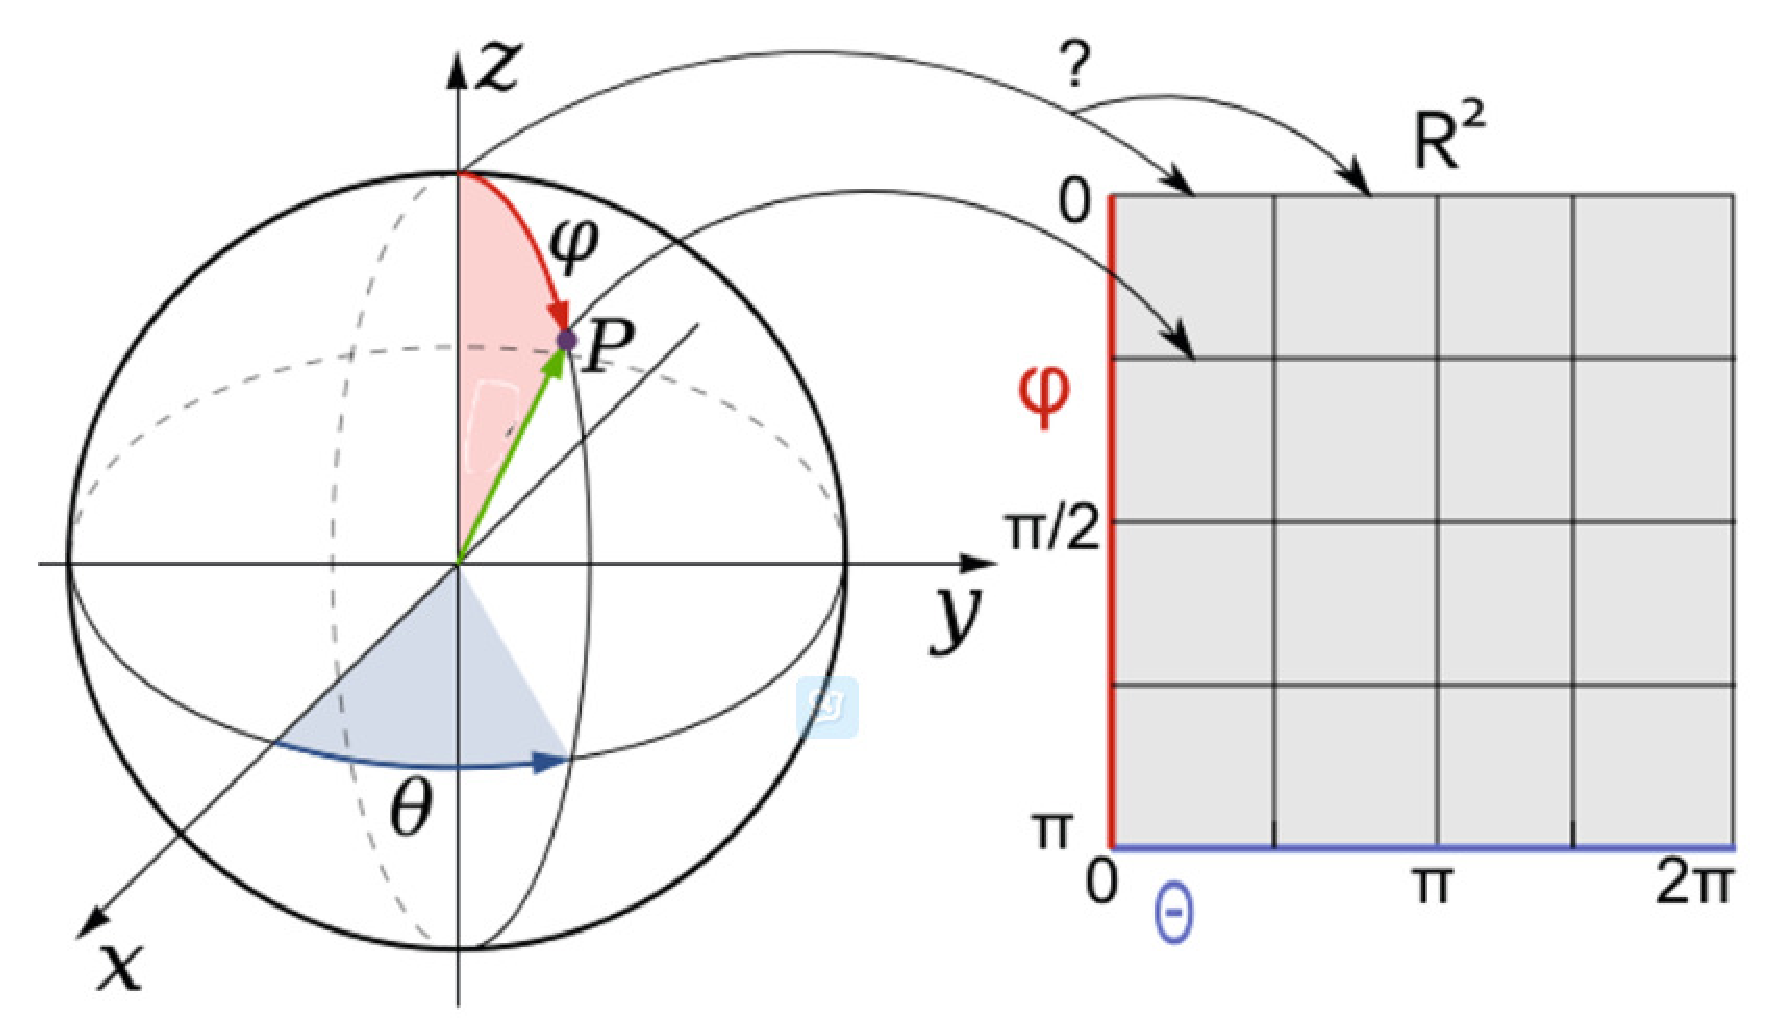
\includegraphics[scale=0.35]{fig3_8.pdf}
    \figcaption{从球面的一个邻域到$\mathbb{R}^2$映射的图示}
}
球面上几乎所有的点都可明确地对应于坐标$(\varphi, \theta)$,几乎所有... 但是极点$\varphi = 0$映射到哪儿?不可能有一对一的点,因为极点对应的是一整条线,在上图已经画出。因此球坐标映射不能覆盖整个球面,还需要一个映射将极点及其邻域映射到$\mathbb{R}^2$。相似的问题还出现在$\theta = 0$对应的半圆处,$\theta = 0$与$\theta = 2\pi$映射到$\mathbb{R}^2$的同一个点,因此也不是一一映射。这说明对流形而言,一般不存在一个覆盖流形所有点的全局坐标系,而只有局域坐标系,即仅覆盖某一邻域的坐标系。不过这没关系,因为流形的特征是局部像$\mathbb{R}^n$。

上面说到,球坐标系映射只对开邻域$0 < \varphi < \pi, 0 < \theta < 2\pi$有效,还需要另外的映射来覆盖整个球面。可以使用第二个球坐标系——坐标轴的指向不同,使得有问题的极点不再对应$\varphi = 0$,在第二个映射补充下,球面上所有的点都可映射到$\mathbb{R}^2$,于是2-球面确实是个流形。

流形的平凡例子是$\mathbb{R}^n$,根据定义容易看出。

%!TEX root = ./../main.tex
%!TEX encoding = UTF-8 Unicode

%——————————————————————————————————————————————————————————
%	CHAPTER 4
%	translator: lh1962
%	proofreader: InSight, SI, laserdog
%——————————————————————————————————————————————————————————
\newcommand\rd{\mathrm d}
\newcommand\ri{\mathrm i}

\chapter[理论框架]{The Framework 理论框架}\label{chap4}
这一章的基本思路是,我们要通过使{\it 某些东西}取极小值,得到正确的关于自然的方程。{\it 某些东西}是什么?至少我们知道一件事:它不应该在 Lorentz 变换下改变,否则我们会在不同的参考系下得到不同的自然规律。在数学意义上,它意味着我们寻找的这个东西是个标量,依照 Lorentz 群的 \( (0,0) \) 表示作变换。再加上到自然对简单规律的偏好,导出关于自然的方程绰绰有余。

从这个想法出发,我们将会引入{\bf 拉格朗日形式(Lagrangian formalism)}。通过使理论的中心对象取极小值,可以得到用以描述问题中的物理系统的运动方程。极小化过程的结果被称作 {\bf 欧拉-拉格朗日方程(Euler-Lagrange equations)}。

通过拉格朗日形式,可以得到物理中最重要的定理之一:{\bf Noether 定理(Noether's Theorem)}。这个定理揭示了对称性和守恒量%
\mpar{守恒量指的是不随时间变化的物理量。例如一个给定体系的能量或动量。数学上意味着\(\rd Q/\rd t = 0 \rightarrow Q = \text{常数}\)。}%
之间的深刻联系。我们将在下一章中利用它来理解,理论是如何来描述实验测量量的。

\section[拉格朗日形式]{Lagrangian Formalism \quad 拉格朗日形式}\label{sec4.1}

拉格朗日形式是在基础物理中被广泛运用的一个强有力的框架%
\mpar{物理中当然有其他框架,例如以{\bf 哈密顿量(Hamiltonian)}为中心对象的{\bf 哈密顿形式(Hamiltonian formalism)}。哈密顿量的问题在于它不是洛伦兹不变的,因为它所代表的能量,仅仅是{\bf 协变能动矢量(covariant energy-impulse vector)}的一个分量}%
。由于理论的基本对象——{\bf 拉格朗日量(Lagrangian)}是一个标量%
\mpar{标量指依照洛伦兹群的 \( (0,0) \) 表示作变换的对象。这意味着它不在洛伦兹变换下改变}%
,它相对简单。如果你希望从对称性的观点考虑问题,这种形式将会是非常有用的。要求拉格朗日量的积分,{\bf 作用量(action)},在某些对称变换下不变,即保证了体系的动力学遵从该对称性。

\subsection{Fermat 原理}\label{sec4.1.1}
\begin{quote}
自然界中不论发生什么过程,由此造成作用量的改变总尽可能的小。


\begin{flushright}
- Pierre de Maupertius
\mpar{Recherche des loix du mouvement (1746)}
\end{flushright}
\end{quote}

拉格朗日形式的思想源于 Fermat 原理:光在两空间点间传播总依耗时最短的路径\(q(t)\)而行。数学上来讲,如果我们定义给定路径\(q(t)\)的作用量为
\[
S_{\text{light}}[{\mathbf q}(t)] = \int ~{\mathrm d}t
\]
而我们的任务便是找到一条特定的路径\(q(t)\)使作用量取极小值%
\mpar{此处的作用量仅仅是沿给定路径对时间的积分,但一般而言作用量会更加复杂,我们待会儿就能见到}%
为了得到一个给定{\bf 函数}的极小值%
\mpar{一般而言,我们希望找到{\bf 极值(extremums)},即极小值{\bf 和}极大值。下一节中的方法足以找到这两者。无论如何,我们将继续谈论极小值}%
,我们可以求得其导函数并令其为零;而为了找到{\bf 泛函}\(S[{\mathbf q}(t)]\)\footnote{译者注:这里的$q(t)$原文一会儿用粗体,一会不用,不知道想表达什么,此处与原文保持一致。}——函数\({\mathbf q}(t)\)的函数\(S\)——的极小值,就得要一个新的数学工具:{\bf 变分法}。

\picmpar{
	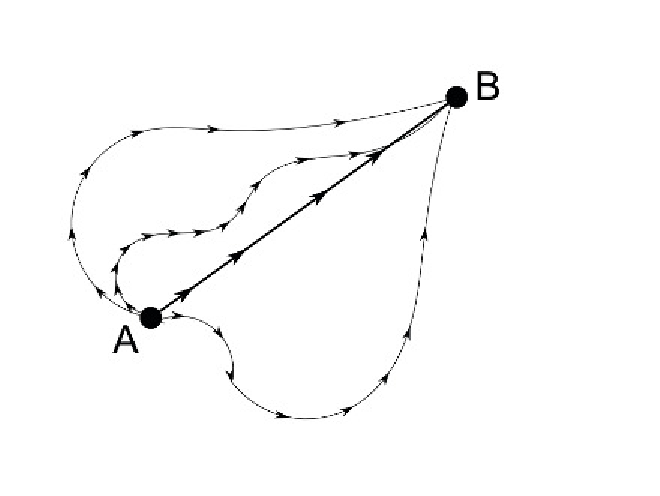
\includegraphics[scale=0.35]{./Figure/fig4_1}
	\caption{对于给定初末端点的路径的扰动}
}

\subsection{变分法:基本思想}\label{sec4.1.2}

在思考如何发展一套能够找到泛函极值的新理论之前,我们需要倒回去想想什么给出一个数学上的极小点。变分法给出的答案是,极小点由极小点邻域的性质决定。例如,让我们尝试寻找一个寻常函数\(f(x)=3x^2+x\)的极小点\(x_{\min}\)。我们从一个特定点\(x=a\)出发,仔细考察其邻域。数学上它意味着\(a + \epsilon\),其中\(\epsilon\)代表无穷小量(可正可负)。我们将\(a\)的变分代入函数\(f(x)\):
\[
f(a+\epsilon) = 3(a+\epsilon)^2+(a+\epsilon) = 3(a^2+2a\epsilon+\epsilon^2)+a+\epsilon \text{。}
\]
如果\(a\)是极小点,\(\epsilon\)的一阶变分必须为零,否则我们可以取\(\epsilon\)为负\(\epsilon < 0\),这样\(f(a+\epsilon)\)就会比\(f(a)\)更小%
\footnote{\textcolor{red}{译注:此处讨论有误。可改作“否则若$\epsilon$的一阶变分为正,我们可以\dots ,反之亦然。”}}%
。因此,我们将线性依赖于\(\epsilon\)的项取出并令其为零。
\[
3 \cdot 2a\epsilon + \epsilon \overset{\text{!}}{=} 0 \rightarrow 6a+1\overset{\text{!}}{=}0\text{。}
\]
由此我们找到极小点
\[
x_{\min} = a = -\frac{1}{6} \text{,}
\]
它自然和我们求导\(f(x)=3x^2+x\rightarrow f'(x)=6x+1\)并令其为零的办法得到的结果一致。对于寻常函数而言,这只是一个用来干同一件事不同方法而已%
\footnote{译注:对于受微元法茶毒的物竞生而言,求导才是用来干这件事的不同方法。}%
,但是变分法却能找到泛函的极值点。我们马上就能看到,应当如何处理一个一般的作用量泛函。

拉格朗日形式的中心思想在于,对于有质量的物体也存在一个与光的 Fermat 原理相类似的原理。当然,它不可能直接遵从费马原理,但是我们可以从一个更一般的形式出发
\[
S[q(t)]=\int {\mathcal L}~{\mathrm d}t
\]
其中\(\mathcal L\)一般是一个非常数的参量,称为拉格朗日量。对于光而言,这个参量是个常数。一般的,拉格朗日量依赖于物体的坐标和速度\({\mathcal L}={\mathcal L}(q(t),\frac{\partial}{\partial t} q(t))\)。下一节中我们将仔细讨论这件事%
\mpar{我们的任务是找到对于给定拉格朗日量和初始条件有着最小作用量的路径\(q(t)\)。在此之前,我们得先找到正确的拉格朗日量,用以描述问题中的物理系统。这是我们在上一章中所讨论的对称性所能发挥作用的地方。通过要求拉格朗日量在洛伦兹群的所有变换下不变,我们就能找到正确的拉格朗日量}%
。在仔细讨论如何对这样一个泛函使用变分法之前,我们需要先讲讲两个小问题。

\section[限制]{Restrictions \quad 限制}\label{sec4.2}
正如\ref{sec1.1}节所提到的,现有理论中有些限制条件无法从第一性原理中得到。我们所能知道是,如果想得到一个有意义的理论,我们必须加上这些限制。

一个重要的限制是,我们仅允许拉格朗日量中出现尽可能低阶的非平凡%
\footnote{译注:原文为`non-trival'. Trival 这个词常包含简单、弱智、无意义之义。}%
导数。这里平凡指的是对于系统的动力学,即运动方程,没有影响。某些理论会包含一阶导数,另外一些带二阶导数。一个给定理论所含的最低阶导数由该条件决定:拉格朗日量在 Lorentz 变换下不变%
\mpar{实际上,作用量才应该是 Lorentz 不变的。但如果拉格朗日量满足这个条件,那作用量自然也是。}%
,否则我们将在不同的参考系下导出不同的运动方程%
\footnote{\textcolor{red}{译注:此处讨论疑有误,作者此前并没有说明积分中的时间是坐标时还是固有时}}%
。对于某些理论,我们无法写出一个仅含一阶导数项的不变量,那么此时二阶导数便成了最低阶导数项。

我们并不清楚如何处理包含高阶导数的理论,它们有一些深刻的、系统性的困难%
\mpar{这些困难称为 Ostrogradski 不稳定性,即包含高阶导数的系统的能量没有下界,以至于系统中的所有态总会自发衰变到能量更低的态上去。这类系统中找不到稳定的状态。}%
。另外,拉格朗日量中的高阶导数会使得运动方程中也包含高阶导数,这样就必须知道更多的初始条件才能决定物体的运动。

有些人会宣称对理论所包含导数阶数的限制源于我们希望得到一个局域%
\mpar{局域性是狭义相对论的基本假定,\ref{sec2.4}节已作阐述}%
理论,但这个要求仅会排除掉那些无穷阶导数。一个非局域相互作用有如下形式%
\mpar{我们将会讨论粒子的拉格朗日理论:寻求粒子的路径;也会讨论场的拉格朗日理论:寻求场函数\(\Phi(x)\)。这将是下一节的主题。}
\begin{equation}
\Phi(x-h)\Phi(x)
\end{equation}
即,时空中距离为\(h\)的两个点的场相互作用。利用 Taylor 展开我们有%
%与前面章节一致,订正公式错误不用红色
\footnote{译注:此式有误,已更正}
\begin{equation}
\Phi(x-h) = \sum\limits_{k=0}^{\infty}\left(\left(\frac{\partial}{\partial x}\right)^k\left.\Phi(x)\right|_{x}\right) \frac{(-h)^k}{k!}
\end{equation}
即包含无穷阶导数会导致一个非局域的理论。

另外一个限制是,要得到一个自由(无相互作用)场/粒子的理论,我们只能写到二次项。这意味着我们只会考虑%
\mpar{从另外一个角度来看,这再次表示我们只引入最低阶的非平凡项。我们随后就会看到,含\(\Phi^0\)和\(\Phi^1\)的项是平凡的,因此我们这次用的是\(\Phi\)的最低阶非平凡项}
\[
\Phi^0, \Phi^1, \Phi^2
\]
这样的项。例如,形如\(\Phi^2 \partial_\mu \Phi\)的项是\(\Phi\)的三阶项,因而不会被包含在我们自由理论的拉格朗日量中。

\section[粒子理论与场论]{Particle Theories vs. Field Theories \quad 粒子理论与场论}\label{sec4.3}
我们目前有两套用以描述自然的理论框架。一套是粒子理论,用依赖于时间的粒子位置描述物理系统,即\(\vec{q}=\vec{q}(t)\)。由于我们不是非得在使用笛卡尔坐标系%
\mpar{例如,我们可以用球坐标系}%
,所以用的是字母\(q\)而不是\(x\)。对于这样的理论,拉格朗日量依赖于坐标\(\vec{q}\),速度\(\partial_t\vec{q}\)和时间\(t\):%
\footnote{译注:严格说来,依赖于坐标函数\(\vec{q}(t)\),速度函数\(\partial_t\vec{q}(t)\)和时间\(t\)}
\begin{equation}
{\mathcal L} = {\mathcal L} (\vec{q},\partial_t\vec{q},t)
\end{equation}

一个著名的拉格朗日量是\({\mathcal L} = \frac{1}{2}m\vec{q}^2\),它能导出经典力学中的 Newton 运动方程。在稍后将进行相当详细的讨论。

另一套是场论:使用场而不是独立粒子的坐标来描述自然%
\mpar{量子场论有一个特别优美的性质是关于如何引进粒子的。我们将在第\ref{chap6}章中看到场有能力产生和湮灭粒子}%
。在这套理论中,时空构成了场\(\Phi(\vec{x},t)\)表演的舞台。利用前面提到过的限制,我们得到%
\mpar{这里我故意使用了不同的符号\({\mathscr L}\),因为在场论中大多数时候我们都在和拉格朗日量密度\({\mathscr L}\)打交道。两者之间满足关系式\({\mathcal L} = \int{\mathrm d}^3\bm{x}~{\mathscr L}\)}
\begin{equation}
{\mathscr L} = {\mathscr L} (\Phi(\vec{x},t), \partial_\mu \Phi(\vec{x},t), \vec{x})
\end{equation}

这里一个著名的拉格朗日量密度\({\mathscr L} = \frac{1}{2}\left(\partial_\mu\Phi\partial^\mu\Phi-m^2\Phi^2\right)\),它可以导出 Klein-Gordon 方程。

场论的一大优点是它将时空等价的对待。在粒子理论中我们使用空间坐标\(\vec{q}(t)\)作为时间的函数来描述粒子。尤其是,拉格朗日量中没有类似于\(\partial_{\vec{q}}t\)的项(如果出现了这类项,我们该怎样理解它呢?)当我们讨论粒子的坐标时,意义是清楚的,但对时间做类似的陈述时,却很难有明确的意义%
\footnote{译注:利用不那么古老的相对论性语言,粒子理论下时空坐标是可以在形式上被同等对待的:用以求导的东西只能是曲线的参数,它可以取作粒子世界线的固有时、某一坐标系的坐标时、或者其他什么东西(只要性质合适,也可以是空间坐标);而时空坐标则被同样的求导。}。

讨论了这么多,我们终于可以回到这章开头所说的极小化问题上来了。我们希望找到某些泛函
\[
S[q(t)] = \int {\mathcal L}~{\mathrm d}t
\]
的极小值,以得到正确的运动方程。

对于粒子而言,方程的解是使得泛函取极小值的正确路径;而对于场而言,解是正确的场函数。

此刻请不用担心\(\mathcal L\)的具体形式,下面数章将详细讨论如何对问题中的系统导出正确的拉格朗日量\({\mathcal L}\)。现在,我们将使用之前所介绍过的变分法,对于一个一般的\(\mathcal L\)导出泛函\(S[q(t)]\)的极小值。极小化过程将给出系统的运动方程。

\section[欧拉-拉格朗日方程]{Euler-Lagrange equation \quad 欧拉-拉格朗日方程}\label{sec4.4}
我们从粒子理论出发,它能让我们搞清楚,在给定初末端点后,粒子是如何在两点间运动的。数学上,即寻找{\bf 函数}\(q(t)\)使得作用量\footnote{译注:此处${\mathcal L}$原文字体有误,已更正}
\[
S = \int_{t_1}^{t_2} {\mathcal L}\left(q(t),\frac{\rd q(t)}{\rd t},t\right)
\]
取极值(极大值或极小值)。

使用记号
\[
\dot q(t) = \frac{\rd q(t)}{\rd t}\text{。}
\]
与之前的例子类似,取\(q(t)=a(t)\)并让对这个函数进行一个扰动
\[
a(t) + \epsilon(t)
\]
其中\(\epsilon\)依旧是一个无穷小量。对于一个粒子而言,我们必须同时改变其速度\(\dot a(t) + \dot\epsilon(t)\),其中\(\dot\epsilon(t) = \frac{\rd \epsilon(t)}{\rd t}\)。

在边界上,扰动后的路径应与原路径相同:
\begin{equation}
0 = \epsilon(t_1) = \epsilon(t_2)
\label{equ4.5}
\end{equation}
这是因为我们寻找的是使作用量积分取极值的{\bf 给定初末端点}的路径。

这个扰动使得泛函变为
\[
S = \int_{t_1}^{t_2} {\mathcal L}\left(q+\epsilon,\dot q + \dot \epsilon, t\right)~\rd t \text{。}
\]
与之前的例子类似,极小值要求线性依赖于扰动\(\epsilon\)的项为零。由于我们处理的是一般的\(\mathcal L\),故将其展开成 Taylor 级数%
\mpar{我们使用的是这个公式的多变量形式,参见附录\ref{appendix.B.3}:
\[
\begin{aligned}
{\mathcal L}\left(q+\epsilon,\dot q + \dot \epsilon, t\right) = {\mathcal L}(q,\dot q,t) + \\
\epsilon\frac{\partial \mathcal{L}}{\partial q} + \dot\epsilon\frac{\partial \mathcal{L}}{\partial \dot q} + \dots
\end{aligned}
\]}%对原文公式有改动
,并令一阶项为零
\begin{equation}
\int_{t_1}^{t_2} \rd t ~ \left[ \epsilon(t) \frac{\partial \mathcal{L}}{\partial q} + \left( \frac{\rd}{\rd t} \epsilon(t) \right)\frac{\partial \mathcal{L}}{\partial \dot q} \right] \overset{\text{!}}{=} 0 \text{。}
\label{equ4.6}
\end{equation}
对后一项做分部积分%
\mpar{分部积分是莱布尼兹律的直接推论,详见附录\ref{appendix.B.2}}%
得到
\[
\begin{aligned}
\int_{t_1}^{t_2} \rd t ~ \left( \frac{\rd}{\rd t} \epsilon(t) \right)\frac{\partial \mathcal{L}(q,\dot q,t)}{\partial \dot q} =\\
\left.\epsilon(t)\frac{\partial \mathcal{L}(q,\dot q,t)}{\partial \dot q}\right|_{t_1}^{t_2} - \int_{t_1}^{t_2} \rd t ~  \epsilon(t) \frac{\rd}{\rd t} \left( \frac{\partial \mathcal{L}(q,\dot q,t)}{\partial \dot q} \right)
\end{aligned}
\]
利用\eqref{equ4.5}式有
\[
\left.\epsilon(t)\frac{\partial \mathcal{L}(q,\dot q,t)}{\partial \dot q}\right|_{t_1}^{t_2} = 0
\]
因此,我们可以将\eqref{equ4.6}改写为
\[
\int_{t_1}^{t_2} \rd t ~\epsilon(t) \left[ \frac{\partial \mathcal{L}}{\partial q} - \frac{\rd}{\rd t} \left( \frac{\partial \mathcal{L}(q,\dot q,t)}{\partial \dot q}\right) \right] \overset{\text{!}}{=} 0
\]
易见上式对于任意扰动\(\epsilon(t)\)为零仅当方括号\([~]\)内的表达式为零。故有%
\mpar{可能你会对于两类不同的导数符号感到困惑。\(\frac{\rd}{\rd t}\)被称作对\(t\)的全导数,而\(\frac{\partial}{\partial t}\)被称为偏导数。全导数给出总改变量,函数\(f\)的变化率,即偏导数,乘以变量自身的改变,之和。
例如,三维空间中的函数\(f(x(t),y(t),z(t))\)的总变化率为\(\frac{\rd f}{\rd t} = \frac{\partial f}{\partial x}\frac{\partial x}{\partial t}+\frac{\partial f}{\partial y}\frac{\partial y}{\partial t}+\frac{\partial f}{\partial z}\frac{\partial z}{\partial t}\)。
即变化率乘以自身的改变量。
相对的,偏导数仅给出总改变量的一部分。对于一个不显式的依赖于\(t\)的函数,其偏导数为零。例如,对于\(f(x(t),y(t))=x^2y+y^3\),我们有\(\frac{\partial f}{\partial t}=0\),但\(\frac{\partial f}{\partial x}=2xy \ne 0, \frac{\partial f}{\partial y}=x^2+3y^2 \ne 0\)。
因此\(\frac{\rd f}{\rd t}=2xy\frac{\partial x}{\partial t}+(x^2+3y^2)\frac{\partial y}{\partial t}\)。
作为对比,对于另一个函数\(g(x(t),y(t),t)=x^2t+y\)我们有\(\frac{\partial g}{\partial t}=x^2\)
}
\begin{equation}
\frac{\partial \mathcal{L}}{\partial q} - \frac{\rd}{\rd t} \left( \frac{\partial \mathcal{L}(q,\dot q,t)}{\partial \dot q} \right)= 0
\label{equ4.7}
\end{equation}
这就是著名的{\bf 欧拉-拉格朗日方程(Euler-Lagrange equation)}

我们可以用类似的办法处理场论。首先,注意到场论将时空同等对待。因此引入拉格朗日量密度:
\begin{equation}
{\mathcal L} = \int{\mathrm d}^3\bm{x}~{\mathscr L}(\Phi^i,\partial_\mu \Phi^i)
\end{equation}
并用拉格朗日量密度来表示作用量
\begin{equation}
S = \int \rd t~{\mathcal L} = \int{\mathrm d}^4\bm{x}~{\mathscr L}(\Phi^i,\partial_\mu \Phi^i)
\end{equation}
依照上面讲过的步骤,我们可以得到场的运动方程组%
\footnote{不对$i$求和}
\mpar{在这里用“组”字是因为对于每一个场分量\(\Phi^1,\Phi^2,\dots\)我们都可以得到一个方程}%
:
\begin{equation}
\frac{\partial \mathscr{L}}{\partial \Phi^i} - \partial_\mu \left( \frac{\partial \mathscr{L}}{\partial (\partial_\mu \Phi^i)} \right)= 0
\label{equ4.10}
\end{equation}

下一节中将在拉格朗日形式下导出近代物理学中重要的一个定理。从中可以看到对称性与守恒量之间的深刻联系。守恒量是描述自然的合适参量%
\mpar{我们将其视做锚定这个复杂的世界之物。不论万事万物如何改变,守恒量依旧是守恒量。}%
,这个定理将教会我们如何和它打交道。

\section[Noether 定理]{Noether's Theorem \quad Noether 定理}\label{sec4.5}
Noether 定理表示,拉格朗日量的每一个对称性都直接对应一个守恒量。换言之,物理学家用于描述自然(守恒量)的记号和对称性直接相关。这确实是科学史上最美的创见之一。

\subsection{粒子理论的Noether 定理}\label{sec4.5.1}
先看看能对粒子理论中的守恒量做点什么。我们限于讨论连续对称性,这样才能使用无穷小变换。如同上一章所言,重复进行无穷小变换可以得到一个有限变换。拉格朗日量在无穷小变换%
\mpar{用符号\(\delta\)来表述小扰动,希望不会和用来表述偏导数的\(\partial\)相混淆。}%
\(q\rightarrow q'=q+\delta q\)下不变的性质用数学表述如下%
\footnote{译者注:该书中$\delta S$,$\delta {\mathcal L}$与平常的约定都差了一个负号。}
\begin{equation}
\begin{aligned}
\delta {\mathcal L} &= {\mathcal L}(q,\frac{\rd q}{\rd t},t) - {\mathcal L}(q+\delta q,\frac{\rd (q+\delta q)}{\rd t},t) \\
&= {\mathcal L}(q,\frac{\rd q}{\rd t},t) - {\mathcal L}(q+\delta q,\frac{\rd q}{\rd t}+\frac{\rd \delta q}{\rd t},t) \overset{\text{!}}{=} 0
\end{aligned}
\label{equ4.11}
\end{equation}

要求拉格朗日量是变换不变的,这个限制太强了。为了保证动力学性质一样,要求不变的应该是作用量而不是拉格朗日量。当然,如果拉格朗日量不变,作用量自然不变:
\begin{equation}
\delta S = \int \rd t~{\mathcal L}(q,\frac{\rd q}{\rd t},t) -  \int \rd t~{\mathcal L}(q+\delta q,\frac{\rd q}{\rd t},t) = \int \rd t~\delta{\mathcal L}\underbrace{=}_{\mathclap{\text{若}~\delta{\mathcal L}=0}} 0
\end{equation}
在什么情况下,拉格朗日量改变而作用量不变呢?答案是,给拉格朗日量加上一个任意函数$G$对时间的全导数
\[
{\mathcal L}\rightarrow{\mathcal L}+\frac{\rd G}{\rd t}
\]
这时作用量不变%
\mpar{用到了$\delta G =\frac{\partial G}{\partial q}\delta q$。这是因为$G=G(q)$而我们改变了$q$,故$G$的扰动等于改变率$\frac{\partial G}{\partial q}$乘上$q$的扰动}
\[
\delta S \rightarrow \delta S' = \delta S + \int_{t_1}^{t_2} {\rd t~\frac{\rd}{\rd t}\delta G} = \delta S + \underbrace{\left.\frac{\partial G}{\partial q} \delta q \right|_{t_1}^{t_2}}_{\mathclap{=0~\text{因为}~\delta q(t_1)=\delta q(t_2)=0}}.
\]
最后一步中用到了扰动$\delta q$在初末时刻\footnote{译注:右侧删去了原文的一对括号,原文为$(t_1,t_2)$}$t_1,t_2$为零。由此可知,拉格朗日量的扰动$\delta {\mathcal L}$不必非要为零,而仅需满足一个更弱的条件
\begin{equation}
\delta {\mathcal L} \overset{\text{!}}{=} \frac{\rd G}{\rd t}\text{。}
\label{equ4.13}
\end{equation}

这意味着拉格朗日量可以在不改变作用量和运动方程的情况下,加减某个函数的全微分$\frac{\rd G}{\rd t}$。将\eqref{equ4.11}式的右端由$0$改作$\frac{\rd G}{\rd t}$,我们有
\begin{equation}
\delta {\mathcal L} =  {\mathcal L}(q,\frac{\rd q}{\rd t},t) - {\mathcal L}(q+\delta q,\frac{\rd q}{\rd t}+\frac{\rd (\delta q)}{\rd t},t) \overset{\text{!}}{=} \frac{\rd G}{\rd t}
\end{equation}
将第二项按 Taylor 级数展开到$\delta q$的一阶项,并使用记号$\frac{\rd q}{\rd t}=\dot q$
\begin{equation}
\begin{aligned}
&\rightarrow \delta {\mathcal L} =  {\mathcal L} - {\mathcal L} -\frac{\partial \mathcal L}{\partial q} \delta q - \frac{\partial \mathcal L}{\partial \dot q} \delta \dot q \overset{\text{!}}{=} \frac{\rd G}{\rd t}  \\
&\rightarrow \delta {\mathcal L} =  -\frac{\partial \mathcal L}{\partial q} \delta q - \frac{\partial \mathcal L}{\partial \dot q} \delta \dot q \overset{\text{!}}{=} \frac{\rd G}{\rd t}
\end{aligned}
\label{equ4.15}
\end{equation}
利用欧拉-拉格朗日方程\mpar{\eqref{equ4.7}式:$\frac{\partial \mathcal L}{\partial q} = \frac{\rd}{\rd t} \left(\frac{\partial \mathcal L}{\partial \dot q}\right)$}重写\eqref{equ4.15}式,有
\[
\rightarrow \delta {\mathcal L} =  -\frac{\rd}{\rd t} \left(\frac{\partial \mathcal L}{\partial \dot q}\right) \delta q - \frac{\partial \mathcal L}{\partial \dot q} \delta \dot q \overset{\text{!}}{=} \frac{\rd G}{\rd t}
\]
利用莱布尼兹律\mpar{如果你对莱布尼兹律仍有疑问,请参考附录\ref{appendix.B.1}},我们有
\begin{equation}
\begin{aligned}
&\rightarrow \delta {\mathcal L} =  -\frac{\rd}{\rd t} \left(\frac{\partial \mathcal L}{\partial \dot q}\delta q\right) \overset{\text{!}}{=} \frac{\rd G}{\rd t} \\
&\rightarrow\frac{\rd}{\rd t} \underbrace{\left(\frac{\partial \mathcal L}{\partial \dot q}\delta q + G\right)}_{\equiv J} \overset{\text{!}}{=} 0
\end{aligned}
\label{equ4.16}
\end{equation}
由此得到了一个不随时间变化的物理量$J$:
\begin{equation}
J = \frac{\partial \mathcal L}{\partial \dot q}\delta q + G\text{,}
\end{equation}
这是因为
\[
\frac{\rd J}{\rd t} = 0 \rightarrow J = \text{常数。}
\]

为了看清楚这一点,先借用一下后面章节的结论:常质量自由粒子的 Newton 第二定律是%
\mpar{如果$q$代表某个物体的位置,则$\frac{\rd q}{\rd t}=\dot q$是这个物体的速度,$\frac{\rd}{\rd t}\frac{\rd q}{\rd t}=\frac{\rd^2 q}{\rd t^2}=\ddot q$是加速度。}
\begin{equation}
m{\ddot{\vec{q}}} = 0 \text{。}
\end{equation}
相应的拉格朗日量是%
\mpar{我们现在处理的是高于一维的问题,所以使用矢量$\vec q$和$\vec a$而不是$q$和$a$。}
\begin{equation}
{\mathcal L}=\frac{1}{2}m\dot\vec{q}^2
\end{equation}
你可以将其代入欧拉-拉格朗日方程(\eqref{equ4.7}式)中去验证它。

让我们从这个拉格朗日量出发,计算不同对称性所分别对应的守恒量。

由于${\mathcal L}=\frac{1}{2}m{\dot\vec q}^2$不依赖于$\vec q$,故此拉格朗日量在空间平移变换$\vec{q}\rightarrow\vec{q}+\vec{a}$不变($\delta{\mathcal L}=0$)。这个对应的守恒量满足条件式\eqref{equ4.13},即$G=0$的情形\footnote{译注:使用了求和约定,见第\ref{chap3}章边注\hyperref[sidenote.3.129]{129}}
\begin{equation}
J_\text{trans} = \frac{\partial\mathcal L}{\partial \dot{\vec q}} \vec a = m {\dot{\vec q}} {\vec a} = \vec{p}\vec{a} \text{,}
\end{equation}
其中$\vec{p}=m{\dot{\vec q}}$是经典力学中的{\bf 动量(momentum)}。由于等式$\frac{\rd J}{\rd t}$对于任意$\vec a$都成立,所以说:{\bf 拉格朗日量的空间平移不变性导致了动量守恒。}

现在考虑旋转变换,这得需要大于一的维度,因为一维上的旋转是没有意义的。下面将不会使用类似$\vec q$的矢量符号,而是更方便的指标记号。我们能将所有方程简单的用$\vec{q}\rightarrow q_i$改写。考虑无穷小旋转%
\mpar{这里我们用 Levi-Civita 符号来写旋转生成元。参见\eqref{equ3.63}式下的文字。}%
$q_i \rightarrow q_i + \epsilon_{ijk} q_j a_k$,由此$\delta q_i=\epsilon_{ijk}q_j a_k$。仍然是因为由于${\mathcal L}=\frac{1}{2}m{\dot\vec q}^2$不依赖于$\vec q$,我们的拉格朗日量在这样的变换下也不改变,其对应的守恒量是%
\mpar{下式由\eqref{equ4.16}式导出,这里对应的依旧是$G=0$的情况}
\begin{equation}
\begin{aligned}
J_\text{rot} =& \frac{\partial {\mathcal L}(q_i, \dot q_i, t)}{\partial \dot q_i}\delta q_i  = \frac{\partial \mathcal L}{\partial \dot q_i} \epsilon_{ijk} q_j a_k \\
  =& m {\dot q_i} \epsilon_{ijk} q_j a_k = m p_i\epsilon_{ijk} q_j a_k \\
  \rightarrow J_\text{rot} =& (\vec{p}\times\vec{q})\cdot\vec{a} \equiv \vec{L}\cdot\vec{a}
\end{aligned}
\end{equation}
在最后一步中我们将表达式用矢量记号重新写出,其中$\times$称作叉乘,而$\vec L$是经典力学中{\bf 角动量(angular momentum)}。即:{\bf 旋转不变性导致了角动量守恒。}

接下来让我们看看时间平移不变性%
\mpar{这意味着物理不会管我们是在昨天、今天还是五十年后做的实验,给定相同的初始条件,物理定律不会变化。}%
。一个无穷小的时间平移$t\rightarrow t'=t+\epsilon$会导致
\begin{equation}
\begin{aligned}
\delta {\mathcal L} &= {\mathcal L}\left(q(t),\frac{\rd q(t)}{\rd t},t\right) - {\mathcal L}\left(q(t+\epsilon),\frac{\rd q(t+\epsilon)}{\rd t},t+\epsilon\right) \\
&= -\frac{\partial \mathcal L}{\partial q}\frac{\partial q}{\partial t}\epsilon -\frac{\partial \mathcal L}{\partial\dot q}\frac{\partial\dot q}{\partial t}\epsilon -\frac{\partial\mathcal L}{\partial t}\epsilon \underbrace{=}_{\mathclap{\text{等式左端正好为全导数}}} -\frac{\rd \mathcal L}{\rd t}\epsilon \text{,}
\end{aligned}
\end{equation}
这表明一般而言$\delta{\mathcal L} \ne 0$,但有$G=-{\mathcal L}$。

将其代入\eqref{equ4.16}式,有\footnote{译注:原文有字体混乱,已更正}
\begin{equation}
\frac{\rd}{\rd t}\underbrace{\left(\frac{\partial\mathcal L}{\partial\dot q}\dot q-{\mathcal L}\right)}_{\equiv\mathcal H} = 0
\end{equation}
守恒量$\mathcal H$称为{\bf 哈密顿量(Hamiltonian)},代表了系统的总能量。对于这个例子,我们有
\begin{equation}
\begin{aligned}
\mathcal H =& \frac{\partial\mathcal L}{\partial\dot q}\dot q-{\mathcal L} = \underbrace{\left(\frac{\partial}{\partial\dot q}\frac{1}{2}m{\dot q}^2\right)}_{\mathclap{=m{\dot q}}}\dot q - \frac{1}{2}m{\dot q}^2 \\
 =& m{\dot q}^2 - \frac{1}{2}m{\dot q}^2 = \frac{1}{2}m{\dot q}^2 \text{,}
\end{aligned}
\end{equation}
正好是系统的动能。由于这里没有势场或外力,故动能就是总能量。能导出在外势场中运动的粒子的 Newton 第二定律$m\ddot q=-\frac{\partial V}{\partial q}$\footnote{\textcolor{red}{原文有误,已更正}}的拉格朗日量是
\[
{\mathcal L} = \frac{1}{2}m{\dot q}^2 - V(q)\text{。}
\]
其哈密顿量为
\[
{\mathcal H} = \frac{1}{2}m{\dot q}^2 + V
\]
的确是正确的总能量(等于动能加势能)。

由{\bf 推动不变性(boost invariance)}导致的守恒量略有些奇怪,相应的计算放在了这一章的附录\ref{sec4.6}中。其结果为
\begin{equation}
\tilde{J}_\text{boost} = \underbrace{pt-\frac{1}{2}mvt}_{\mathclap{\equiv \tilde{p}t}}-mq=\tilde{p}t-mq
\end{equation}
我们可以看到这个量依赖于时间零点,可以通过恰当的选取时间零点使其为零。由于这个量是守恒量,这个守恒律告诉我们零始终都是零。\footnote{译注:这个守恒率没有说的那么平庸,事实上,它等价于质心运动定理;\\ \textcolor{red}{~~~~~\,又注:该结果以及附录\ref{sec4.6}的推导有误,参见\hyperref[note:boost]{译注23}}}
%修改完成后注意调整译注序号!

作为粒子理论的总结,我们得到了如下关系:
\begin{itemize}
\item 空间平移不变性$\Rightarrow$动量守恒
\item 推动不变性\mpar{推动的另一个叫法是动量空间的平移,因为变换$q\rightarrow q+vt$使动量$m\dot q\rightarrow m(\dot q+v)$}$\Rightarrow~\tilde{p}t-mq$守恒
\item 旋转不变性$\Rightarrow$角动量守恒
\item 时间平移不变性$\Rightarrow$能量守恒
\end{itemize}
Noether 定理向我们展示了,为什么这些记号%
\mpar{除了推动不变性导致的守恒量}%
会以这个或那个形式出现在形形色色的物理理论中。只要我们依旧有通常的时空对称性,动量、能量和角动量就是守恒量。在场论中,有两类对称性:一方面,拉格朗日量会在时空变换(如旋转)下不变;另一方面,我们也会有在场自身的变换下的不变性,称为{\bf 内禀对称性(internal symmetries)。}

\subsection{场论中的 Noether 定理——时空对称性}\label{sec4.5.2}
对于场,我们得区分在时空变换下两类不同的改变。当观测者$S$看到场$\Psi(x)$时,观测者$S'$看到的则是场$\Psi'(x')$。这是同一个场,只是从不同的视角来看,会有不同的分量值。这两类描述之间由 Lorentz 群中的一个合适的变换相联系。我们现在将会使用在\ref{sec3.7.11}节中介绍过的场表示%the field representation
。(无穷维)微分算符表示$x$变换到$x'$。这意味着利用这个表示我们能在不同的时空点或者在一个旋转参考系中计算场分量。Lorentz 群的有限维变换使$\Psi$映射到$\Psi'$,即,混合场分量%
\mpar{请回忆这个例子,Weyl 旋量有两个分量而矢量场有四个分量。如果我们从一个不同的视角来考察矢量场$A_\mu=\begin{pmatrix} A_0\\ A_1\\ A_2\\ A_3 \end{pmatrix}$,即,从旋转系看,它会形如$A'_\mu=\begin{pmatrix} A'_0\\ A'_1\\ A'_2\\ A'_3 \end{pmatrix}=\begin{pmatrix} A_0\\ -A_2\\ A_1\\ A_3 \end{pmatrix}$。$A'_\mu$和$A_\mu$描述了从两个相差了绕$z$轴旋转$90^\circ$的坐标系分别观察到的同一个场。}。

对于一个依赖于时空的场的具体变换,需要同时考虑两个部分。我们将分别处理它们,首先来看$x$到$x'$的这一项。对于旋转来说,单由这一个部分推出的守恒量并不会真的守恒,这是因为我们忽略了变换的第二项。仅当将变换的两项$x\rightarrow x'$和$\Psi\rightarrow\Psi'$分别导致的守恒量加起来之后得到的,才是真正守恒的。

为了使上面这段论证更有说服力,我们考虑一个一般的拉格朗日量密度${\mathscr L}\left(\Phi(x_\mu),\partial_\mu \Phi(x_\mu),x_\mu\right)$\footnote{译注:原文多出一左括号}。对称性意味着
\begin{equation}
{\mathscr L}\left(\Phi(x_\mu),\partial_\mu \Phi(x_\mu),x_\mu\right) = {\mathscr L}\left(\Phi'(x'_\mu),\partial_\mu \Phi'(x'_\mu),x'_\mu\right)\text{。}
\end{equation}
一般的,当函数自身发生改变且其计算的点也发生改变时,函数的函数的总改变量由下式给出%
\mpar{如果你对此不熟悉:这常被称为全导数。总改变量等于变化率,即偏导数,乘以变量自身的改变,之和。例如,三维空间中的函数\(f(x,y,z)\)的总该变量为\(\frac{\partial f}{\partial x}\delta x+\frac{\partial f}{\partial y}\delta y+\frac{\partial f}{\partial z}\delta z\),即变化率乘以自身改变的距离。我们考察的是无穷小变化,故我们可以略去 Taylor 展开的高阶项仅考虑第一项。}
\begin{equation}
\delta f(g(x),h(x),\dots)=\frac{\partial f}{\partial g}\delta g + \frac{\partial f}{\partial h}\delta h + \dots +\frac{\partial f}{\partial x}\text{。}
\end{equation}
运用到拉格朗日量上有
\begin{equation}
\delta {\mathscr L} = \frac{\partial\mathscr L}{\partial \Phi}\delta\Phi + \frac{\partial\mathscr L}{\partial(\partial_\mu \Phi)}\delta(\partial_\mu\Phi) + \frac{\partial\mathscr L}{\partial x_\mu}\delta x_\mu\text{,}
\end{equation}
用欧拉-拉格朗日方程\mpar{\eqref{equ4.10}式:\\ $\frac{\partial \mathscr{L}}{\partial \Phi} = \partial_\mu \left( \frac{\partial \mathscr{L}}{\partial (\partial_\mu \Phi)} \right)$}将其改写为
\begin{equation}
\begin{aligned}
\delta {\mathscr L} &= \partial_\mu\left(\frac{\partial\mathscr L}{\partial(\partial_\mu \Phi)}\right)\delta\Phi + \frac{\partial\mathscr L}{\partial(\partial_\mu \Phi)}\underbrace{\delta(\partial_\mu\Phi)}_{\mathclap{=\partial_\mu\delta\Phi}} + \frac{\partial\mathscr L}{\partial x_\mu}\delta x_\mu \\
&\underbrace{=}_{\mathclap{\text{莱布尼兹律}}} \partial_\mu\left(\frac{\partial\mathscr L}{\partial(\partial_\mu \Phi)}\delta\Phi\right) + \frac{\partial\mathscr L}{\partial x_\mu}\delta x_\mu
\end{aligned}
\label{equ4.29}
\end{equation}
其中$\delta\Phi$有两项
\begin{equation}
\delta\Phi = \epsilon_{\mu\nu}S^{\mu\nu}\Phi(x)-\frac{\partial\Phi(x)}{\partial x_\mu}\delta x_\mu \text{,}
\label{equ4.30}
\end{equation}
其中$\epsilon_{\mu\nu}$为旋转参数,$S_{\mu\nu}$为相应的有限维群表示中的旋转算符,额外的负号仅为了方便。$S_{\mu\nu}$是由旋转生成元$S_{i}=\frac{1}{2}\epsilon_{ijk}S_{jk}$和推动生成元$K_i=S_{i0}$构成,类似于\eqref{equ3.165}式中$M_{\mu\nu}$的定义。$S_{\mu\nu}$的这个定义使得我们同时进行旋转和推动。

第一项仅在旋转和推动时较重要,因为平移不会导致场分量的混合。推动所对应的守恒量依旧不是特别有意思,就像在粒子理论中得到的那样。所以实际上这一项只和旋转相关。

让我们从最简单的场变换出发:时空平移,即
\begin{equation}
x_\mu \rightarrow x'_\mu = x_\mu + \delta x_\mu = x_\mu + a_\mu
\label{equ4.31}
\end{equation}
将$\epsilon_{\mu\nu}=0$(在平移下场分量不会混合)代入方程\eqref{equ4.30}
\[
\delta\Phi = -\frac{\partial\Phi(x)}{\partial x_\mu}\delta x_\mu
\]
再由\eqref{equ4.29}式,考察不变性($\delta{\mathscr L}=0$)所导致的守恒量
\begin{eqnarray}
-\partial_\nu\left(\frac{\partial\mathscr L}{\partial(\partial_\nu \Phi)}\frac{\partial\Phi(x)}{\partial x_\mu}\delta x_\mu\right) + \frac{\partial\mathscr L}{\partial x_\mu}\delta x_\mu &= 0 \\
\rightarrow -\partial_\nu\left(\frac{\partial\mathscr L}{\partial(\partial_\nu \Phi)}\frac{\partial\Phi(x)}{\partial x^\mu} - \delta_\mu^\nu{\mathscr L}\right) \delta x^\mu &= 0 \label{equ4.33}
\end{eqnarray}

由\eqref{equ4.31}式我们有$\delta x^\mu = a^\mu$,代入\eqref{equ4.33}式中可得\footnote{译者注:原文上下数式的指标不平衡,现已修正。}
\begin{equation}
-\partial_\nu\left(\frac{\partial\mathscr L}{\partial(\partial_\nu \Phi)}\frac{\partial\Phi(x)}{\partial x^\mu} - \delta_\mu^\nu{\mathscr L}\right) a^\mu = 0 \text{,}
\label{equ4.34}
\end{equation}
我们定义能动张量
\begin{equation}
T_\mu^\nu : = \frac{\partial\mathscr L}{\partial(\partial_\nu \Phi)}\frac{\partial\Phi(x)}{\partial x^\mu} - \delta_\mu^\nu{\mathscr L} \text{。}
\label{equ4.35}
\end{equation}
由于$a_\mu$是任意的,\eqref{equ4.34}式告诉我们$T_\mu^\nu$满足连续性方程
\begin{align}
&\partial_\nu T_\mu^\nu = 0 \label{equ4.36}\\
\rightarrow &\partial_\nu T_\mu^\nu = \partial_0 T_\mu^0 - \partial_i T_\mu^i = 0 \label{equ4.37}
\end{align}
对于所有$\mu$成立。这直接告诉我们有守恒量的存在,例如取$\mu=0$我们有%
\mpar{使用了$\partial_0 = \partial_t$\\ 和$\partial^i T_i^0=\nabla\cdot\vec{T}$,\\以及著名的散度定理$\int_V \rd^3 \bm{x}~\nabla A = \int_{\delta V} \rd^2 \bm{x}~A$,即能让体积分化作面积分。对于散度定理,在那儿叫 Gauss定理,有一个非常有启发性的证明,可以在Richard P. Feynman, Robert B. Leighton, and Matthew Sands.\\ The Feynman Lectures on Physics: Volume 2. Addison-Wesley,\\ 1st edition, 2 1977. \\ISBN 9780201021172 的第三章找到,可在此免费在线查看:\\ \url{http://www.feynmanlectures.caltech.edu/II_03.html}。\\(译注:有中译本:费恩曼,莱顿,桑兹著;李洪芳,王子辅,钟万蘅译.费恩曼物理学讲义,新千年版,第二卷,上海:上海科学技术出版社,4 2013,ISBN 9787547816370)}
\begin{equation*}
\begin{aligned}
\partial_0 T_0^0 - \partial_i T_0^i = 0 \rightarrow \partial_0 T_0^0 = \partial_i T_0^i \\
\partial_t T_0^0 = - \nabla\cdot\vec{T} \underbrace{\rightarrow}_{\mathclap{\text{在某个无限的空间域$V$上积分}}} \int_V \rd^3 \bm{x}~\partial_t T_0^0 = - \int_V \rd^3 \bm{x}~\nabla\cdot\vec{T} %
\end{aligned}
\end{equation*}
\begin{equation}
\partial_t \int_V \rd^3 \bm{x}~T_0^0 = - \int_V \rd^3 \bm{x}~\nabla\cdot\vec{T}\overbrace{\rightarrow}^{\mathclap{\text{散度定理;$\delta V$代表$V$的表面}}} = -\int_{\delta V}\rd^2 \bm{x}~\vec{T} \underbrace{=}_{\mathclap{\text{场在无穷远处为零}}} 0
\end{equation}
\begin{equation}
\rightarrow \partial_t \int_V \rd^3 \bm{x}~T_0^0 = 0 \label{equ4.39}
\end{equation}

最后一步中是这样处理的:考虑一个无限大的空间域,如一个有着无限大半径$r$的球体,我们需要在其表面计算积分,即在$r=\infty$处计算场值。在\ref{sec2.3}节中,我们发现了物理中任何东西都有一个速度上界。由此无穷远处的场不可能对有限远$x$处的物理有任何影响,故我们说场在无穷远处为零\footnote{译注:这段讨论怪怪的,正确性令人起疑。}。

最终的结论是:时空平移不变性导致四个守恒量%
\mpar{因为对于任意$a_\mu$都有$\partial_0 T_\mu^0 a_\mu = \partial_0 T_0^0 a_0 -\partial_0 T_i^0 a^i = 0$成立,所以对于每一个分量我们都能得到一个连续性方程。}%
,\eqref{equ4.39}式告诉我们它们是
\begin{align}
E =& \int\rd^3\bm{x}~T_0^0 \label{equ4.40}\\
P_i =& \int\rd^3\bm{x}~T_i^0 \label{equ4.41}
\end{align}
其中$i=1,2,3$。它们分别被称为系统的总能量——因时间平移$x_0\rightarrow x_0+a_0$不变性而守恒;场的总动量——因空间平移$x_i\rightarrow x_i+a_i$不变性而守恒。

\subsection{旋转和推动}\label{sec4.5.3}
接下来,我们会仔细研究旋转和推动下的不变性。先从\eqref{equ4.30}式的第二项出发,随后讨论第一项的含义。我们将从第一项和第二项分别得到一个量,两项之和是守恒的。标量场没有可以混合的分量,故对于它而言第一项始终为零,即$S_{\mu\nu}=0$;也可以用\ref{sec3.7.4}节的结论解释:我们用标量作为 Lorentz 群一维表示的生成元。故在第一部分中导出的将会是对应于标量场真实守恒量。

变换的第二项由下式给出
\[
x_\mu \rightarrow {x'}_\mu = x_\mu + \delta x_\mu = x_\mu + M_\mu^\sigma x_\sigma
\]
其中$M_\mu^\sigma$是转动和推动的在无穷维表示下的生成元,即在\eqref{equ3.240}式中所定义的微分算符。

将$\delta x_\mu = M_\mu^\sigma x_\sigma$代入\eqref{equ4.33}中得
\begin{eqnarray}
\partial_\nu\left(\frac{\partial\mathscr L}{\partial(\partial_\nu\Phi)}\frac{\partial\Phi(x)}{\partial x^\mu} - \delta_\mu^\nu{\mathscr L}\right) M^{\mu\sigma} x_\sigma = 0 \label{equ4.42} \\
\underbrace{\rightarrow}_{\mathclap{\eqref{equ4.35}\text{式}}} \partial_\nu T_\mu^\nu M^{\mu\sigma} x_\sigma =0 \nonumber
\end{eqnarray}
我们能将它改写成更常见的形式
\begin{eqnarray}
 &=& \frac{1}{2} (\partial^\nu T^\mu_\nu M_{\mu\sigma} x^\sigma + \partial^\nu T^\mu_\nu \underbrace{M_{\mu\sigma}}_{\mathclap{=-M_{\sigma\mu} }} x^\sigma) = \frac{1}{2} (\partial^\nu T^\mu_\nu M_{\mu\sigma}x^\sigma+\partial^\nu T^\mu_\nu - M_{\sigma\mu}x^\sigma) \nonumber\\
 &\underbrace{=}_{\mathclap{\text{替换哑指标}}}& \frac{1}{2}(\partial^\nu T^\mu_\nu M_{\mu\sigma}x^\sigma+\partial^\nu T^\sigma_\nu-M_{\mu\sigma}x^\mu) = \frac{1}{2}(\partial^\nu T^\mu_\nu x^\sigma+\partial^\nu T^\sigma_\nu x^\mu) M_{\mu\sigma} \nonumber\\
 &=&\frac{1}{2}\partial_\nu ( T^{\mu\nu} x^\sigma+\partial^\nu T^{\sigma\nu}x^\mu) M_{\mu\sigma} = 0 \nonumber\\
 &\rightarrow& \text{引入}(J^\nu)^{\sigma\mu} \equiv T^{\mu\nu} x^\sigma-\partial^\nu T^{\sigma\nu}x^\mu \rightarrow \partial_\nu (J^\nu)^{\sigma\mu} = 0 \text{。}
\end{eqnarray}
在最后一步引入的$J^\nu$被称为{\bf Noether 流(Noether current)}。注意到,由于在\eqref{equ3.165}式定义$
M$时引入的反对称性$M_{\mu\sigma}=-M_{\sigma\mu}$,有$M_{\mu\mu}=0$。由此我们找到了六个不同的连续性方程$\partial_\nu (J^\nu) = 0$,分别对应于每一个非零的$M_{\mu\sigma}$\footnote{译注:排除了零元的同时,也将始终互为相反数的一对元视作一个}。使用与\eqref{equ4.39}式一样的方式,我们可以论证如下的量不随时间改变
\begin{equation}
Q^{\mu\sigma} = \int \rd^3 \bm{x}~ \left(T^{\mu 0} x^\sigma- T^{\sigma 0}x^\mu\right)
\end{equation}
由此我们得到了对应于转动%
\mpar{回忆一下\eqref{equ3.165}式中提到的转动生成元$J_i$和$M_{\mu\nu}$之间的关系:$J_i = \frac{1}{2}\epsilon_{ijk}M_{jk}$,这里我们使用拉丁字母$i,j\in \{1,2,3\}$而不是希腊字母$\mu,\nu\in\{0,1,2,3\}$,将其限制在空间分量上。}%
不变性的守恒量
\begin{equation}
L_\text{orbit}^i = \frac{1}{2}\epsilon_{ijk}Q_{jk} = \frac{1}{2}\epsilon_{ijk} \int \rd^3 \bm{x}~ \left(T^{\mu 0} x^\sigma-\partial^\nu T^{\sigma 0}x^\mu\right) \text{,}
\label{equ4.45}
\end{equation}
其被称为场的轨道角动量\mpar{下标 orbit (轨道)的含义马上就会清楚,因为它实际上只是守恒量的一部分,我们马上就会去考察第二项。}。

同样的,我们也有所对应的守恒量\mpar{请回忆推动生成元$K_i$和$M_{\mu\nu}$之间的关系:$K_i=M_{0i}$}
\begin{equation}
Q^{0i}=\int \rd^3 \bm{x}~ \left(T^{i 0} x^0- T^{0 0}x^i\right)
\label{equ4.46}
\end{equation}
将会在附录\ref{sec4.7}节中详细讨论。

\subsection{自旋}\label{sec4.5.4}
接下来我们希望捡回原先在导出守恒量时所丢掉的\eqref{equ4.30}中的第一项。现在考察
\begin{equation}
\delta\Phi = \epsilon_{\mu\nu} S^{\mu\nu}\Phi(x) \text{,}
\end{equation}
其中$S^{\mu\nu}$是问题中的变换%
\mpar{场分量的混合是由有限维表示来进行的。例如转动生成元的二维表示$J_i = \frac{1}{2}\sigma_i$混合了Weyl旋量的分量。}%
的恰当{\bf 有限维表示}表示。这使\eqref{equ4.29}式多了一项
\begin{equation}
\partial_\rho \left(\frac{\partial\mathscr L}{\partial (\partial_\rho \Phi)}\epsilon_{\mu\nu}S^{\mu\nu}\Phi(x)\right)
\end{equation}
同时也使\eqref{equ4.45}式多了一项。完整的守恒量是
\begin{equation}
L^i = \frac{1}{2}\epsilon_{ijk}Q^{jk} = \frac{1}{2}\epsilon_{ijk} \int \rd^3 \bm{x}~ \left(\frac{\partial\mathscr L}{\partial (\partial_0 \Phi)}S^{jk}\Phi(x) + (T^{k 0} x^j-T^{j 0}x^k)\right)
\end{equation}
据此写出
\begin{equation}
L^i = L_\text{spin}^i + L_\text{orbit}^i \text{。}
\end{equation}
第一项是个新东西,但和我们之前考虑的轨道角动量有类似之处,因为这是当我们讨论同一个不变性时出现而加在一起的。标准的观点是这个守恒量是某种内禀%
\mpar{我们随后将会看到场产生湮灭粒子。一个自旋$\frac{1}{2}$场产生自旋$\frac{1}{2}$粒子,这是基本粒子的固有属性。所以说我们用“内禀”这个词。轨道角动量是用来描述两个或更多粒子如何相互旋转的一个量。}%
角动量。

回忆我们曾用某种也叫做自旋(spin)的东西来给 Poincar\'e 群的表示作标签。现在这个记号再一次出现了。我们将在下一章,并在\ref{sec8.5.5}节中相当仔细地,学习如何能测量这类新的角动量,自旋,以及认识到它和我们用以给 Poincar\'e 群的表示作标签的东西,确实是相一致的。

\subsection{场论中的 Noether 定理——内禀对称性}\label{sec4.5.5}
我们现在来仔细研究内禀对称性%
\mpar{毋庸置疑,对于相互作用场论,内禀对称性是相当重要的。除此之外,我们将从最简单的内禀对称性引出的守恒量出发开始学习量子场论}%
。在某些场{\bf 自身}的无穷小变换
\begin{equation}
\Phi_i \rightarrow \Phi'_i = \Phi_i + \delta\Phi_i
\label{equ4.51}
\end{equation}
下拉格朗日量的不变性$({\delta \mathscr L}=0 )$,数学上表达为\footnote{译注:原文上下标混乱,已修改。}
\begin{eqnarray}
\delta {\mathscr L} &=& {\mathscr L}( \Phi_i,\partial_\mu\Phi_i) - {\mathscr L}(\Phi_i+\delta\Phi_i,\partial_\mu(\Phi_i+\delta\Phi_i) ) \nonumber\\
&=& - \frac{\partial\mathscr L}{\partial \Phi_i}\delta\Phi_i - \frac{\partial\mathscr L}{\partial(\partial_\mu \Phi_i)}\partial_\mu\delta\Phi_i \overset{\text{!}}{=} 0 \text{,} \label{equ4.52}
\end{eqnarray}
即因变换是无穷小的,故 Taylor 展开到$\delta\Phi_i$第一项。依场的欧拉-拉格朗日方程\eqref{equ4.10}可知
\[
\frac{\partial \mathscr{L}}{\partial \Phi} = \partial_\mu \left( \frac{\partial \mathscr{L}}{\partial (\partial_\mu \Phi)} \right) \text{。}
\]
代入\eqref{equ4.42}式,我们得到
\begin{equation*}
\delta {\mathscr L} = - \partial_\mu \left( \frac{\partial \mathscr{L}}{\partial (\partial_\mu \Phi_i)} \right)\delta\Phi_i - \frac{\partial\mathscr L}{\partial(\partial_\mu \Phi_i)}\partial_\mu\delta\Phi_i = 0
\end{equation*}
再用上莱布尼兹律,得到
\begin{equation}
\partial_\mu \left( \frac{\partial \mathscr{L}}{\partial (\partial_\mu \Phi_i)} \delta\Phi_i \right) = 0
\label{equ4.53}
\end{equation}

这意味着,如果拉格朗日量在变换$\Phi_i \rightarrow \Phi'_i = \Phi_i + \delta\Phi_i$下不变,那我们又得到一个被称为了 Noether 流的量
\begin{equation}
J^\mu \equiv \frac{\partial \mathscr{L}}{\partial (\partial_\mu \Phi)} \delta\Phi_i \text{,}
\label{equ4.54}
\end{equation}
其满足连续性方程
\begin{equation}
\eqref{equ4.53}\text{式}\rightarrow \partial_\mu J^\mu=0 \text{。}
\end{equation}
更进一步,用导出\eqref{equ4.39}式同样的办法,能得到一个对时间的守恒量
\begin{equation}
\partial_t \int \rd^3 \bm{x}~J^0 = 0 \text{。}
\label{equ4.56}
\end{equation}

我们再来看一个重要的例子:在场自身的平移下不变性%
\mpar{注意此时我们并没有假定场是实的还是复的。常数$\epsilon$是任取的,若我们想让场平移量是实的,我们当然可以令它是虚数。这里用$\ri$是为了使生成元是厄米的(现在来看还没什么意义),这样其本征值就是实的。现在不要太困扰,把这个额外的$\ri$当做是一个约定就好,只要通过定义$\epsilon':=\ri\epsilon$,就能把它吸收到常数里去。}%
,即在\eqref{equ4.51}式中的$\delta\Phi = -\ri\epsilon$:
\begin{equation}
\Phi \rightarrow \Phi' = \Phi -\ri\epsilon \text{。}
\end{equation}
或者对于不止一个分量的场
\begin{equation}
\Phi_i \rightarrow \Phi'_i = \Phi_i -\ri\epsilon_i \text{。}
\end{equation}
%2016/10/5前的稿子漏了一段?
这个变换的生成元是$-i\frac{\partial}{\partial \Phi}$,因为
\begin{equation}
\label{equ4.59}
\Phi'=e^{-i\epsilon \frac{\partial}{\partial \Phi}}\Phi=(1-i\epsilon \frac{\partial}{\partial \Phi}+\dots)\Phi \approx \Phi-i\epsilon
\end{equation}
对应的守恒量被称为{\bf 共轭(conjugate)}动量$\Pi$。方便起见,引入共轭动量密度%
\mpar{这个相当概括的量是量子场论最重要的记号,我们将在第\ref{chap6}章中看到这一点}%
$\pi \equiv J_0$,通过\eqref{equ4.53}、\eqref{equ4.56}式,并利用守恒量中不需要包含$\delta\Phi = -\ri\epsilon$这件事。我们得到%
\mpar{\eqref{equ4.54}式中的$\delta\Phi$成为一个常数$\epsilon$,因为这个量对于任何$\epsilon$都守恒,所以我们在定义守恒量时不需要它。}
\begin{align}
\partial_t \Pi = 0 ~\rightarrow~ \partial_t \Pi = \partial_t\int\rd^3\bm{x}~J_0 = \partial_t\int\rd^3\bm{x}~\pi = 0 \nonumber \\
\text{用到了}~J_0 = \pi = \frac{\partial \mathscr{L}}{\partial (\partial_0 \Phi)}
\label{equ4.60}
\end{align}

注意这和源于{\bf 空间}平移不变性$\Phi(x)\rightarrow\Phi(x')=\Phi(x+\epsilon)${\bf 物理的}场动量密度不同,那东西长这样
\[
p^i = T^{0i} = \frac{\partial \mathscr{L}}{\partial (\partial_0 \Phi)} \frac{\partial\Phi}{\partial x_i} \text{,}
\]
即之前在\eqref{equ4.41}式中导出的东西。下面数章中我们将会看到更多不同的内禀对称性,它们在发展相互作用理论时是无价的。现在来总结一下我们学过的场论中的对称性和守恒量:
\begin{itemize}
\item 空间平移不变性$\Rightarrow$ 物理动量\\$P^i = \int\rd^3\bm{x}~T^{0i}=\int\rd^3\bm{x}~ \frac{\partial \mathscr{L}}{\partial (\partial_0 \Phi)} \frac{\partial\Phi}{\partial x_i}$守恒
\item 推动不变性\mpar{推动又被称为在动量的空间平移}$\Rightarrow$ 能量中心的速度是常数
\item 转动不变性$\Rightarrow$ 总角动量\\$L^i =\frac{1}{2}\epsilon_{ijk} \int \rd^3 \bm{x} \left(\frac{\partial\mathscr L}{\partial (\partial_0 \Phi)}S^{jk}\Phi(x) + (T^{k0} x^j-T^{j0}x^k)\right) $\\$= L_\text{spin}^i + L_\text{orbit}^i $,包含自旋和轨道角动量,守恒
\item 时间平移不变性$\Rightarrow$ 能量\\$E = \int\rd^3\bm{x}~T^{00}=\int\rd^3\bm{x}~\left(\frac{\partial \mathscr{L}}{\partial (\partial_0 \Phi)} \frac{\partial\Phi}{\partial x_i}-\mathscr{L}\right)$守恒
\item 场自身的平移不变性$\Rightarrow$ 共轭动量\\$\Pi = \int\rd^3\bm{x}~\frac{\partial \mathscr{L}}{\partial (\partial_0 \Phi)} = \int\rd^3\bm{x}~\pi$守恒
\end{itemize}

\section*{Further Reading Tips\quad 阅读建议}
\begin{itemize}
\item {\bf Cornelius Lanczos - The Variational Principles of Mechanics}%
\mpar{Cornelius Lanczos. The Variational Principles of Mechanics. Dover Publications, 4th edition, 3 1986. ISBN 9780486650678}%
是一本关于拉格朗日体系在经典力学中的应用的绝妙的书。
\item {\bf Herbert Goldstein - Classical Mechanics}%
\mpar{Herbert Goldstein, Charles P. Poole Jr., and John L. Safko. Classical Mechanics. Addison-Wesley, 3rd edition, 6 2001. ISBN 9780201657029}%
是经典力学的标准教材,其中有许多对拉格朗日体系非常好的解释。
\end{itemize}
\section[附录:粒子理论中的推动不变性与其守恒量]{Appendix: Conserved Quantity from Boost Invariance for Particle Theories\quad 附录:粒子理论中的推动不变性与其守恒量}\label{sec4.6}
此附录中我们想找到对于示例拉格朗日量${\mathcal L}=\frac{1}{2}m \dot\vec{q}^2 $其来自于推动不变性的守恒量。一个推动变换即$q\rightarrow q'=q+\delta q=q+vt$,其中$v$代表一个常值速率。该拉格朗日量在推动下并不是不变的,但正如之前就看到过的,这并不是一个问题:\\
为了使运动方程在变换下不变,拉格朗日量至多允许变化一个任意函数的全导数。这个条件在推动变换$q\rightarrow q'=q+vt \underbrace{\Rightarrow}_{\mathclap{v=\text{常数!}}} \dot q'=\dot q+v$下是显然满足的,即我们的拉格朗日量
\begin{equation*}
{\mathcal L}=\frac{1}{2}m \dot q^2
\end{equation*}
的改变量为
\begin{equation}
\begin{aligned}
\delta {\mathcal L} &={\mathcal L}(q,\dot q,t)-{\mathcal L}(q',\dot q',t) =\frac{1}{2}m \dot q^2 - \frac{1}{2}m \dot q'^2\\
&= \frac{1}{2}m \dot q^2 - \frac{1}{2}m (\dot q+v)^2 = -mq\dot v - \frac{1}{2}mv^2\text{,}
\end{aligned}
\end{equation}
等于下面这个函数的全导数%
\mpar{$\frac{\rd G}{\rd t} =\frac{\rd}{\rd t}(-mqv -\frac{1}{2}mv^2 t)=-mq\dot v - \frac{1}{2}mv^2$,因为$v$和$m$都是常数。}
\begin{equation*}
G \equiv -mqv -\frac{1}{2}mv^2 t\text{。}
\end{equation*}
我们断言运动方程%
\mpar{看到这一点的另一个方法是直接看运动方程:$m\ddot q=0$。我们有变换$q\rightarrow q'=q+\delta q=q+vt$,其中$v$是常数,且有$\dot q\rightarrow \dot q'=\dot q+v$以及$\ddot q\rightarrow \ddot q'=\ddot q$。}%
不变%
\mpar{拉格朗日量改变了,即$\delta {\mathcal L}\ne 0$,但是作用量值最多改变一个全导数,故我们得到了相同的运动方程。}%
,故我们找到了一个守恒量。

对于推动,守恒量是(\eqref{equ4.16}式)\footnote{译注:原文中下式有符号错误,已改正。}
\begin{equation*}
J_\text{boost} = \underbrace{\frac{\partial \mathcal L}{\partial \dot q}}_{\mathclap{\equiv p} }\underbrace{\delta q}_{\mathclap{=vt} } + G = pvt-mvq-\frac{1}{2}mv^2t\text{,}
\end{equation*}
由于$\eqref{equ4.16}$式右端为零,故我们能除去一个$v$的公因子%
\footnote{\textcolor{red}{译注:由于之前关于守恒量的诸多推导都使用了变换是无穷小变换这一条件,故这里$v$必须取无穷小量,即略去$J_\text{boost}$中$v$的二阶项,最后得到的才能是守恒量。否则再利用其它条件我们会得到$t\equiv 0$的荒谬结论。}\label{note:boost}}%
。由此有
\begin{equation}
\tilde{J}_\text{boost} = \underbrace{pt-\frac{1}{2}mvt}_{\mathclap{\equiv \tilde{p}t} }-mq=\tilde{p}t - mq
\end{equation}
这是一个奇怪的守恒量,因为它的值依赖于时间零点的选取。我们能选择一个合适的时间零点使得这个量为零。由于它是守恒量,故这个零始终是零。

\section[附录:场论中的推动不变性与其守恒量]{Appendix: Conserved Quantity from Boost Invariance for Field Theories\quad 附录:场论中的推动不变性与其守恒量}\label{sec4.7}
由场论中的推动不变性,我们有如下守恒量
\begin{equation}
Q^{0i}=\int \rd^3 \bm{x}~ \left(T^{i 0} x^0- T^{0 0}x^i\right)\text{,}
\end{equation}
即在\eqref{equ4.46}式中所导出的,利用了$K_i=M_{0i}$。

我们怎样诠释这个守恒量呢?$Q^{0i}$是守恒的,意味着
\begin{equation*}
\begin{aligned}
0= \frac{\partial Q^{0i}}{\partial t} &= \underbrace{\int \rd^3 \bm{x}~ \frac{\partial T^{i0}}{\partial t} x^0}_{\mathclap{=x^0\frac{\partial}{\partial t}}} + \int \rd^3 \bm{x}~ T^{i 0} \underbrace{\frac{\partial x^0}{\partial t}}_{\mathclap{=1~\text{因为}~x^0=t} }  - \frac{\partial}{\partial t}\int \rd^3\bm{x}~T^{00}x^i \\
&= t\frac{\partial P^i}{\partial t} + P^i - \frac{\partial}{\partial t}\int \rd^3\bm{x}~T^{00}x^i
\end{aligned}
\end{equation*}
由\eqref{equ4.41}式\footnote{译注:原文公式引用有误,已改正。}可知$P^i$是守恒的$\frac{\partial P^i}{\partial t}=0\rightarrow P^i=\text{常量}$,故我们断言
\begin{equation}
\frac{\partial}{\partial t}\int \rd^3\bm{x}~T^{00}x^i = P^i = \text{常数。}
\end{equation}
故这个守恒律告诉我们%
\mpar{不要太在意这一项的意义,因为它并不像其他守恒量那样有用。}%
能量中心以一个恒定的速度运动。或者从另一个视角来看:动量等于总能量乘以质心速度。

不论如何,\eqref{equ4.46}式中导出的守恒量还是显得很奇怪。它能通过恰当选取起始时刻而取作零。我们能选择一个合适的时间零点使得这个量为零。由于它是守恒量,故这个零始终是零。\footnote{译注:很是不能理解作者的意思。毕竟我们可以选取合适的能量零点使能量为零、合适的惯性系使动量为零、以及合适的匀速转动系使角动量为零。其他的守恒量并没有更优越的地方。}


%!TEX encoding = UTF-8 Unicode

\part{The Equations of Nature \\ 自然界的方程}

\begin{partquote}
{\bfseries “如果你正在从给方程添加美感的方面考虑,你就在成功的路上了。”}\marginpar{``If one is working from the point of view of getting beauty into one's equation,\dots one is on a sure line of progress.''}


\begin{flushright}
--- Paul A. M. Dirac\\
in {\itshape The evolution of the
physicist's picture of nature.}
\marginpar{%
Scientific American,\\vol.208
Issue 5,pp.45-53.\\
Publication Date: 05/1963
}
\end{flushright}
\end{partquote}

%!TEX encoding = UTF-8 Unicode

%----------------------------------------------------------------------------------------
%   CHAPTER 5
%   Translator: laserdog
%   Proofreder: SI
%----------------------------------------------------------------------------------------

\chapterimage{chapter_head_1.pdf} % Chapter heading image

\begin{quote}%quote for every part.I have trouble inserting it into the part cover,so it's now there as a workaround.If you have a better way,please tell me.
{\bf “如果你正在从给方程添加美感的方面考虑,你就在成功的路上了。”}\marginpar{"If one is working from the point of view of getting beauty into one’s equation,...one is on a sure line of progress."}


\begin{flushright}
--- Paul A. M. Dirac\\
in {\it The evolution of the
physicist's picture of nature.}
\marginpar{%
Scientific American,\\vol.208
Issue 5,pp.45-53.\\
Publication Date: 05/1963
}
\end{flushright}
\end{quote}

\chapter[测量]{Measuring Nature 测量}\label{chap5}

现在已经发现对称性与守恒量之间的关系了,接下来就可以利用这种联系。用更专业的话说,Noether定理建立了对称变换的生成元与相应守恒量之间的联系。本章将利用这种联系。

守恒量常常被物理学家们用来描述物理系统,因为无论这个系统经历了怎样复杂的变化,守恒量都是一样的。比如,物理学家们为了描述一个实验会使用动量,能量或角动量。Noether定理提示了一个至关重要的思想:描述自然的物理量等同于其对应的生成元:

\begin{align}\label{equ5.1}
\text{物理量}\Rightarrow\text{对应对称性的生成元}
\end{align}

我们会看到这种选择会自然地导出量子理论。下面通过考虑粒子理论来实现。

\section[量子力学中的算符]{Operators of Quantum Mechanics 量子力学中的算符}\label{sec5.1}

{\it 惯例用一个尖帽子$\hat{O}$来表示一个算符}

拉格朗日量在空间平移变换的生成元的作用下不变可导出动量守恒。因此,由此可得\footnote{译者注:这里再次提醒一下,本书中虚数单位与指标经常共用字母$i$,相信聪明的读者有能力分辨。}
\[\text{动量}\hat{p}_i\to\text{空间平移操作的生成元:} - i\partial_i \]

类似的,时间平移生成元带来的不变性给出能量守恒,也就是
\[\text{能量}\hat{E}\to\text{时间平移操作的生成元} - i\partial_0 \]

没有关于``位置守恒''的对称性,所以位置并没有伴随生成元,我们有\mpar{或者说,我们可以观察守恒量与对应的推动下的不变性。注意到我们在\ref{sec4.6}节中得到的非相对论性Galilei推动下的守恒量是从非相对论性的拉格朗日量得出来的。同样,我们可以对相对论性拉格朗日量做一样的事情,得到守恒量$t\vec{p}-\vec{x}E$。相对论性能量由$E=\sqrt{m^2+p^2}$给出。在相对论性极限$c\to\infty$下,我们有$E\approx m$,并且,Lorentz推动下的守恒量回到我们的Galilei推动的结果。因此,粒子理论的守恒量为$M_i = (tp_i-x_iE)$。推动的生成元(见\eqref{equ3.240},其中$K_i = M_{0i}$)为$K_i = i(x_0\partial_i-x_i\partial_0)$。比较两者,其中$x_0=t$,给出$M_i = (tp_i-x_iE)\leftrightarrow K_i = i(t\partial_i-x_i\partial_0)$。因此,利用我们之前的选择,很直观的我们有,坐标:$\hat{x}_i\to x_i$}
\[\text{位置}\hat{x}_i\to x_i \]

上面利用算符给出了描述自然的理论中使用的物理量。接下来我们自然要问:这些算符作用在什么上面?它们是如何与实验中的可观测量联系起来的呢?下一章仔细讨论这件事情,在这里只需要知道物理量,也就是算符,是作用在{\it 某物}上的。不妨就认为它作用于一个抽象的对象上,称之为$\Psi$,后面会探究这个“{\it 某物}”是什么鬼。

现在可以导出一些非常重要的\mpar{如果你完全不了解量子力学,为什么这些简单的式子会如此重要对你来说会看起来比较奇怪。你也许听说过Heisenberg不确定性原理。在第\ref{sec8.3}节,我们会更进一步的研究量子力学的形式与结构,然后就可以看到这个方程表明不能够以任意精度同时测量一个粒子的动量和坐标。我们的物理量的解释是算符的测量,而这个方程告诉我们先测量动量再测量位置与先测量位置再测量动量是完全不一样的。}量子力学的方程了。就像上面已经解释过的那样,我们假定算符作用在抽象的$\Psi$上。于是有
\begin{align}\label{equ5.2}
\begin{split}
[\hat{p}_i, \hat{x}_j] \Psi &= (\hat{p}_i \hat{x}_j - \hat{x}_j \hat{p}_i) \Psi = i(-\partial_i \hat{x}_j + \hat{x}_j \partial_i) \Psi \\
&\underbrace{=}_{\mathclap{\text{莱布尼兹律}}} -i(\partial_i \hat{x}_j) \Psi - \cancel{i\hat{x}_j (\partial_i \Psi)} + \cancel{i\hat{x}_j (\partial_i \Psi)} \underbrace{=}_{\mathclap{\partial_i \hat{x}_j = \frac{\partial x_j}{\partial x_i}}} -i \delta_{ij} \Psi
\end{split}
\end{align}

这个方程对任意的$\Psi$都成立,因为我们没有对$\Psi$做任何假设,因此我们可以不考虑它\mpar{如果你以前没有过这个观念,注意我们可以把{\bf 每}一个矢量方程都写成只包含数的形式。比如,牛顿第二定律$\vec{F} = m\vec{\ddot{x}}$,可以对于任意矢量$\vec{C}$写出$\vec{F}\vec{C} = m\vec{\ddot{x}}\vec{C}$。不仅如此,如果对于任意的$\vec{C}$都成立,那么一直把这个$\vec{C}$写着也就没什么意义了。}而直接的写出
\begin{align}\label{equ5.3}
[\hat{p}_i,\hat{x}_j] = -i\delta_{ij}
\end{align}

\subsection[自旋与角动量]{Spin and Angular Momentum 自旋与角动量}\label{sec5.1.1}

上一章的第\ref{sec4.5.4}节中讲过,对标量理论而言,旋转不变性带来的守恒量有两个部分,第二部分对应轨道角动量,称之为{\bf 无限}维的轨道角动量生成元表示。
\[\text{轨道角动量}\hat{L}_i\to\text{转动生成元(无限维表示)}i\tfrac{1}{2}\epsilon_{ijk}(x^j\partial^k-x^k\partial^j)\]
类似的, 第一部分称作自旋,对应{\bf 有限}维度的生成元\mpar{这是从场的分量的线性组合下的不变性带来的守恒量,因此是有限维的表示。}的表示。
\[\text{自旋}\hat{S}_i\to\text{转动生成元(有限维表示)}S_i \]
如前面\eqref{equ4.30}式解释过的那样,$S_{\mu\nu}$和转动算符生成元$S_i$的关系为$S_i = \tfrac{1}{2}\epsilon_{ijk}S_{jk}$。

比如,当我们考虑自旋$\tfrac{1}{2}$场的时候,我们需要用到我们在\ref{sec3.7.5}节中得到的二维表示:
\begin{align}\label{equ5.4}
\hat{S}_i = i\frac{\sigma_i}{2}
\end{align}
其中$\sigma_i$是Pauli矩阵。在学习如何利用本章导出的这些算符之后,我们在\ref{sec8.5.5}节深入讨论这一有趣而奇怪的类型的角动量。时刻注意,只有这两部分角动量的{\bf 和}是守恒的。

\section[量子场论的算符]{The Operators of Quantum Field Theory 量子场论的算符}\label{sec5.2}

场论的最重要的客体当然就是{\bf 作为时空位置的函数}\mpar{这里,$x = x_0,x_1,x_2,x_3$,包含时间$x_0=t$。}的场了$\Phi = \Phi(x)$。我们接下来希望描述时空上的一个点发生的相互作用,从而我们需要考虑动力学变量$\pi = \pi(x)$的密度,而不是其其总量$\Pi = \int d^3x\pi(x)\neq\Pi(x)$。

我们上一章发现了场自身的平移不变性$\Phi\to\Phi-i\epsilon$产生了一种新的守恒量,称为共轭动量$\Pi$。就像我们上一章做的那样,我们用对应的生成元\eqref{equ4.59}式来表示共轭动量密度:
\[\text{共轭动量密度}\pi(x)\to\text{关于场自身平移的生成元:}-i\frac{\partial}{\partial\Phi(x)} \]
后面会看到量子场论与这里处理的稍稍不同,而现在的处理已经足够了。

就像上一节讨论的那样,我们需要给算符一些作用的对象。这里同样使用抽象的$\Psi$,后面的章节会具体说明。同样可以得到一个针对量子场论\mpar{最后一步的时候我们类似$\tfrac{\partial x_i}{\partial x_j} = \delta_{ij}$给出delta分布$\tfrac{\partial f(x_i)}{\partial f(x_j)} = \delta(x_i-x_j)$,它实际上可以严格的说明的。更具体的内容请看附录D.2。}十分重要的方程。
\begin{align}\label{equ5.5}
\begin{split}
[\Phi(x),&\pi(y)]\Psi = \left[\Phi(x),-i\frac{\partial}{\partial\Phi(y)}
\right]\Psi\\
\underbrace{=}_{\text{莱布尼兹律}}\cancel{-i\Phi(x)\frac{\Psi}{\partial\Phi(y)}} +& \cancel{i\Phi(x)\frac{\Psi}{\partial\Phi(y)}} + i\left(\frac{\partial\Phi(x)}{\partial\Phi(y)}\right)\Psi = i\delta(x-y)\Psi
\end{split}
\end{align}

同样的,由于这个式子对任意的$\Psi$都成立,可以写成:
\begin{align}\label{eq5.6}
[\Phi(x),\pi(y)] = i\delta(x-y)
\end{align}
类似的,对于场有多于一个分量的情况,我们有
\begin{align}\label{eq5.7}
[\Phi_i(x),\pi_j(y)] = i\delta(x-y)\delta_{ij}
\end{align}

后面我们会看到,几乎所有的量子场论的内容都要从这个简单的方程出发。

%!TEX encoding = UTF-8 Unicode

%----------------------------------------------------------------------------------------
%	CHAPTER 6
%       translator: laserdog
%       proofreader: Surgam Identidem
%----------------------------------------------------------------------------------------

\chapterimage{chapter_head_1.pdf} % Chapter heading image

\chapter[自由场理论]{Free Theory \quad 自由场理论}\label{chap6}

本章建立{\bfseries 自由}体系的物理理论,也就是说无相互作用的情况下的对称性给出的场\mpar{尽管这里针对的是场,后面会看到这里得到的方程同样可以用来处理粒子}。我们会
\begin{itemize}
\item 利用Lorentz群的$(0,0)$表示给出Klein-Gordon方程
\item 利用Lorentz群的$(\tfrac{1}{2},0)\oplus(0,\tfrac{1}{2})$表示给出Dirac方程
\item 利用Lorentz群的矢量$(\tfrac{1}{2},\tfrac{1}{2})$表示给出Proca方程,在无质量极限下退化到著名的Maxwell方程组
\end{itemize}

\section[Lorentz协变性与不变量]{Lorentz Covariance and Invariance \quad Lorentz协变性与不变量}\label{sec6.1}

本章会导出粒子物理的标准模型(这是我们拥有的最好的物理理论)中的运动方程。我们期待这些方程在所有的惯性系中都一样,因为如果不这样的话,每一个参考系都有各自的方程,而狭义相对论指出并没有一个特别的参考系,所以各惯性系中方程形式相同。这称为{\bfseries Lorentz协变性}。一个Lorentz协变的对象是说它按照某一种给定的Lorentz群的表示来进行变换。比如说,矢量$A_\mu$,通过$\left(\frac{1}{2},\frac{1}{2}\right)$表示变换,因此是Lorentz协变的;这其实是说,Lorentz变换:$A_\mu \to A'_\mu$,$A_\mu, A'_{\mu}$实际是同一个对象(而非完全不同的)。另一方面,比如说,$A_1+A_3$就不是Lorentz协变的,因为它不按照Lorentz群的某种表示来变换。但这并不是说我们不知道它是如何变换的,因为它的变换规律从$A_\mu$的变换规律里面可以简单地得出,但是在不同的惯性系中它看起来完全不一样。经推动变换到另一个惯性系之后它看起来或许像$A_2+A_4$。只包含Lorentz协变的对象的方程称为Lorentz协变方程,比如
\[A_\mu+7B_\mu+C_\nu A^\nu D_\mu = 0 \]
就是一个Lorentz协变方程,因为在另一个参考系中,它看起来就是
\[A_\mu+7B_\mu+\underbrace{C_\nu A^\nu}_{\mathclap{=\text{一个Lorentz标量,根据$(0,0)$表示来进行变换}}} D_\mu = A'_\mu+7B'_\mu+C_\nu A^\nu D'_\mu = 0 \]
它在不同惯性系看起来是一样的。只有一部分是这样的方程一般不是Lorentz协变的,它在另一个惯性系里面会不一样。

为了导出Lorentz{\bfseries 协变}的方程,我们要求作用量$S$是Lorentz{\bfseries 不变}的。这是说$S$只能包含在参考系变换下保持不变的成分。换句话说,作用量里面只可以包含Lorentz变换下不变的成分。从作用量$S$中我们可以得到运动方程\mpar{回忆一下,我们使作用量取极小值进而得到的欧拉-拉格朗日方程就是系统的运动方程。}。如果$S$依赖于参考系,那么运动方程就不是Lorentz协变的了。

就像前一章提到的,可以用更严格的约束条件——要求拉格朗日量是Lorentz不变的,这样作用量也就肯定是不变的了。

\section[Klein-Gordon 方程]{Klein-Gordon Equation \quad Klein-Gordon 方程}\label{sec6.2}

下面从最简单的情况开始:标量,它按照Lorentz群的$(0,0)$表示变换。我们要找出对应的拉格朗日量来确定标量的运动方程。符合要求的拉格朗日量的一般形式为\mpar{在\ref{sec4.2}节中有所讨论:我们只考虑$0, 1$和$2$阶的$\Phi$。只考虑最低可能的导数项的原因在后面就会说明。}:

\begin{align}
\label{equ6.1}
\mathscr{L} = A\Phi^0+B\Phi+C\Phi^2+D\partial_\mu\Phi+E\partial_\mu\Phi\partial^\mu\Phi+F\Phi\partial_\mu\Phi
\end{align}
注意我们考虑的是拉格朗日量密度$\mathscr{L}$而不是$L$本身,物理理论从作用量
\begin{align}
\label{equ6.2}
S = \int d\mathbf{x} \mathscr{L}
\end{align}
得出,其中$d \mathbf{x}$可以理解为对时间和空间的积分。因此,诸如$\Phi\partial_\mu\partial^\mu\Phi$的项实际是没必要的,因为它等效于$\partial_\mu\Phi\partial^\mu\Phi$,从分部积分就可以直接看出\mpar{分部积分产生的边界项为零,因为在远处场很小。值得注意的是,这是由于我们物理里面的速度是有上限的(第\ref{sec2.3}节)。因此,很远处的场对于有限远的$x$位置的场不会有影响。}。

不仅如此,Lorentz{\bfseries 不变性}要求拉格朗日量必须是标量。因此,所有奇数阶的$\partial_\mu$,比如$\partial_\mu\Phi$是禁止的。值得一提的是,如果常数,比如$a, c$,有一个Lorentz指标的话,这说明这些常数是一个$4$-矢量,标定了时空的方向从而破坏了空间的各向同性。常数项实际上可忽略,也就是$A=0$,因为物理理论从欧拉-拉格朗日方程中导出,因此一个常数项对运动方程没有影响\mpar{考虑\eqref{equ4.10}式:\[\frac{\partial{\mathscr{L}}}{\partial\Phi}-\partial_\mu\left(\frac{\partial{\mathscr{L}}}{\partial(\partial_\mu\Phi)}\right) = 0\]因此$\mathscr{L}\to\mathscr{L}+A$中的常数项$A$并不改变任何东西:$\frac{\partial({\mathscr{L}}+A)}{\partial\Phi}-\partial_\mu\left(\frac{\partial({\mathscr{L}}+A)}{\partial(\partial_\mu\Phi)}\right) = \frac{\partial{\mathscr{L}}}{\partial\Phi}-\partial_\mu\left(\frac{\partial{\mathscr{L}}}{\partial(\partial_\mu\Phi)}\right)$.}。除此之外,我们可以忽略掉$\Phi$的线性项,也就是说$B=0$,因为从欧拉-拉格朗日方程中可以看出这一项只会给运动方程增加一个常数\mpar{$\mathscr{L}\to\mathscr{L}+B\Phi$使得\\$\frac{\partial(\mathscr{L}+B\Phi)}{\partial\Phi}-\partial_\mu\left(\frac{\partial(\mathscr{L}+B\Phi)}{\partial(\partial_\mu\Phi)}\right)=\frac{\partial\mathscr{L}}{\partial\Phi}-\partial_\mu\left(\frac{\partial{\mathscr{L}}}{\partial(\partial_\mu\Phi)}\right)+B=0$,只产生运动方程中的可加常数。}。那么,剩下的项就是:
\begin{align}
\label{equ6.3}
\mathscr{L}=C\Phi^2+E\partial_\mu\Phi\partial^\mu\Phi
\end{align}

本章开始就指明了要建立一个自由场的理论,这意味着只有一个$\Phi$而不会有形如$\Phi_1\Phi_2$这种相互作用形式,这样的项在下一章——描述相互作用的理论中考虑。

还有一件事情需要注意:最后留下了两个常数$C$和$E$,利用变分法可以把它俩最终收为一个常数,因为拉格朗日量整体差一个常数因子并无影响\mpar{$\mathscr{L}\to C\mathscr{L}$得到
\[\begin{split}
\frac{\partial(C\mathscr{L})}{\partial\Phi}&-\partial_\mu\left(\frac{\partial(C\mathscr{L})}{\partial(\partial_\mu\phi)}\right)=0\\
&\updownarrow\\
\frac{\partial(\mathscr{L})}{\partial\Phi}&-\partial_\mu\left(\frac{\partial(\mathscr{L})}{\partial(\partial_\mu\phi)}\right)=0
\end{split} \]}。不仅如此,通常我们都在拉格朗日量前增加一个$\frac{1}{2}$,然后称另外的常数\mpar{后面我们就会明白的看到为什么这样称呼这个常数:它正是拉格朗日量中的粒子质量。}为$-m^2$。因此,我们最终得到了
\begin{align}
\label{equ6.4}
\mathscr{L}=\frac{1}{2}(\partial_\mu\Phi\partial^\mu\Phi-m^2\Phi^2)
\end{align}

现在利用变分法,也就是说把拉格朗日量带入到欧拉-拉格朗日方程\eqref{equ4.10}式,我们就得到了运动方程
\begin{align}
\label{equ6.5}
\begin{split}
&\frac{\partial\mathscr{L}}{\partial\Phi}-\partial_\mu\left(\frac{\partial(\mathscr{L})}{\partial(\partial_\mu\Phi)}\right)=0\\
&\rightarrow\frac{\partial}{\partial\Phi}\left(\frac{1}{2}(\partial_\mu\Phi\partial^\mu\Phi-m^2\Phi^2)\right)-\partial_\mu\left(\frac{\partial}{\partial(\partial_\mu\Phi)}\left(\frac{1}{2}(\partial_\mu\Phi\partial^\mu\Phi-m^2\Phi^2)\right)\right)=0 \\
&\rightarrow(\partial_\mu\partial^\mu+m^2)\Phi=0
\end{split}
\end{align}

这就是著名的{\bfseries Klein-Gordon方程},是描述自旋$0$的自由场/粒子的方程。

\subsection[复Klein-Gordon场]{Complex Klein-Gordon Field \quad 复Klein-Gordon场}\label{sec6.2.1}

%有点自作主张的改了$L$的字体,不知是否妥当。
对于自旋$0$的场可以不用标量场的复共轭构造Lorentz不变的拉格朗日量。然而对于自旋$\frac{1}{2}$场$\Psi$来说就不一样了,这会带来非常有趣的结果\mpar{剧透:每个自旋$\frac{1}{2}$的粒子都有反粒子。用复数场实际上就是同时考虑两个场,接下来会说到。因此,我们强制的令Lorentz不变性同时在{\bfseries 两个}(紧密联系的)场上作要求,这通常就解释为粒子和反粒子场。}。而且,我们甚至也可以像很多教科书一样研究等价的Lorentz不变的拉格朗日量
\[\mathscr{L}=\partial_\mu\phi^\dagger\partial^\mu\phi-m^2\phi^\dagger\phi \]
这实际上与考虑{\bfseries 两个}等质量标量场的相互作用是一样的:
\[\mathscr{L}=\frac{1}{2}\partial_\mu\phi_1\partial^\mu\phi_1-\frac{1}{2}m^2\phi_1^2+\frac{1}{2}\partial_\mu\phi_2\partial^\mu\phi_2-\frac{1}{2}m^2\phi_2^2 \]
因为我们有
\[\phi\equiv\frac{1}{\sqrt2}(\phi_1+i\phi_2) \]
Lorentz对称性决定了拉格朗日量的形式。基本的标量(自旋$0$)粒子非常罕见,事实上,只有Higgs玻色子是实验上验证了的,但是这个拉格朗日量可以描述复合系统,比如介子。因此,下面不再研究这种拉格朗日量了,而且大多数教科书中也仅仅是用它来作为习题。

\section[Dirac方程]{Dirac Equation \quad Dirac 方程}\label{sec6.3}
\begin{quote}
Dirac的另一个故事是他第一次遇到Feynman的时候,在漫长的寂静之后他说:“我有一个方程。你也有吗?”\\
\phantom{Dirac的另一个故事是他第一次遇到}---{\bfseries Anthony Zee\mpar{Anthony Zee.\\{\itshape Quantum Field Theory in a Nutshell}. Princeton University Press, 1st edition, 3 2003. ISBN 9780691010199}}
\end{quote}

我们这节想要研究自由的自旋$\frac{1}{2}$场/粒子的运动方程。我们会使用Lorentz群的$(\frac{1}{2},0)\oplus(0,\frac{1}{2})$表示,因为要描述宇称变换下的对称性的理论必须同时有$(\frac{1}{2},0)$和$(0,\frac{1}{2})$表示\mpar{我们在第\ref{sec3.7.9}节中说明了,宇称变换会把$(\frac{1}{2},0)$表示变成$(0,\frac{1}{2})$表示}。而在这种对称群表示下做变换的对象称为Dirac旋量,包括右手旋量和左手旋量。\ref{sec3.7.9}节讲过,Dirac旋量定义为
\begin{align}
\label{equ6.6}
\Psi\equiv\left(\begin{matrix}\chi_L\\ \xi_R\end{matrix}\right)=\left(\begin{matrix}\chi_a\\ \xi^{\dot{a}}\end{matrix}\right)
\end{align}

现在需要用Dirac旋量构造某个Lorentz不变量,从而放到拉格朗日量里面。第一步是从左手旋量和右手旋量出发构造不变量。

利用在第\ref{sec3.7.7}节介绍的Van-der-Waerden记号。两种可能的形式分别是\mpar{这里实际上有另外两种可能,称为Majorana质量项。我们已经知道如何使用自旋“度规”$\epsilon$来把自旋指标升或者降。我们可以写一个Lorentz不变的项,诸如$\epsilon(\xi_L)^\dagger\xi_L$,因为$\epsilon(\xi_L)^\dagger=\xi^a$的形式,有一个上标的右手旋量;但是这样写的话就会缺少自由度。$\chi_R$和$\xi_L$都有两个分量,因此我们在诸如$(\chi_R)^\dagger\xi_L$的项里面有四个自由度,而在$\epsilon(\xi_L)^\dagger\xi_L=\xi^a\xi_a$中,像右手旋量一样变换的东西并不依赖于$\xi_L$,我们从而只有两个自由度。关于Majorana旋量实际上还有很多可以说的,它到现在还在进行(实验上的)研究来确定中微子到底属于哪一种。再多说一句,Majorana旋量是``实''的Dirac旋量。这里我打引号的原因是通常实的就是说$\Psi^\star\overset{!}{=}\Psi$。对于旋量来说,这个条件并不Lorentz协变(因为Lorentz变换的表示是复的)。如果我们强制要求我们的标准要求($\Psi^\star\overset{!}{=}\Psi$)的话,对于换一个参考系这事情一般来说就不对了。然而,我们还是给一个对Dirac旋量的Lorentz协变的``实''条件:$\left(\begin{matrix}0&\epsilon\\-\epsilon&0\end{matrix}\right)\Psi^\star\overset{!}{=}\Psi$,二者通常诠释为电荷共轭。这种诠释在第\ref{sec7.1.5}中会进行解释。因此,Majorana旋量实际上描述的是一种粒子,它的电荷共轭粒子,通常叫反粒子,就是它自己。Majorana粒子是自己的反粒子,而Majorana旋量就是Dirac旋量再加一个附加条件:$\Psi_M\equiv\left(\begin{matrix}\xi_L\\\epsilon\xi_L^\star\end{matrix}\right)$或$\Psi_M\equiv\left(\begin{matrix}-\epsilon\chi_R^\star\\\chi_R\end{matrix}\right)$}:
\begin{align}
\label{equ6.7}
I_1:=\chi_{\dot{a}}^T\xi^{\dot{a}}=(\chi_a^\star)^T\xi^{\dot{a}}=(\chi_a)^\dagger\xi^{\dot{a}}=(\chi_L)^\dagger\xi_R
\end{align}
和
\begin{align}
\label{equ6.8}
I_2:=(\xi^a)^T\chi_a=((\xi^a)^\star)^T\chi_a=(\xi_R)^\dagger\chi_L
\end{align}
\ref{sec3.7.7}节讲过,Lorentz不变量总是要把带点的下标和带点的上标,或者不带点的下标和不带点的上标结合。这里再次看到右手旋量和左手旋量需要成对出现。

更进一步的,我们可以构造两种组合,其涉及到一阶导数且满足Lorentz协变,我们一会儿就会看到。但是首先需要理解旋量的导数意味着什么。\ref{sec3.7.8}节讲过如何从旋量构造4-矢量
\[v_{a\dot{b}}=v_\nu\sigma^\nu_{a\dot{b}} \]
其中$v_\nu$像4-矢量一样变换。因此,旋量表述下的导数算符就是
\begin{align}
\label{equ6.9}
\partial_{a\dot{b}}=\partial_\nu\sigma^\nu_{a\dot{b}}
\end{align}

惯例上会定义$\bar\sigma^0=I_{2\times2},\bar\sigma^i=-\sigma^i$,因此我们可以构建Lorentz不变的项
\begin{align}
\label{equ6.10}
I_3:=(\chi_{\dot{a}})^T\partial_\mu(\sigma^\mu)^{\dot{a}b}\chi_b=(\chi_L)^\dagger\partial_\mu\bar\sigma^\mu\chi_L
\end{align}
和
\begin{align}
\label{equ6.11}
I_4:=(\xi^a)^T\partial_\mu(\sigma^\mu)_{a\dot{b}}\xi^{\dot{b}}=(\xi_R)^\dagger\partial_\mu\sigma^\mu\xi_R
\end{align}

除了$(\sigma^\mu)_{a\dot{b}}$之外,我们还需要$(\sigma^\mu)^{a \dot{b}}$。\footnote{原文为$(\sigma^\mu)^{\dot{a} b}$,译文已按勘误表改正。}第一个指标必须是不带点的,第二个指标必须是带点的,这样才可以和其它旋量指标合适的组合。我们通过作用旋量度规两次得到$(\sigma^\mu)^{a\dot{b}}$:
\begin{align}
\label{equ6.12}
\begin{split}
(\sigma^\mu)^{a\dot{b}}&=((\sigma^\mu)^T)^{\dot{b}a}=\epsilon^{\dot{b}\dot{c}}((\sigma^\mu)^T)_{\dot{c}d}(\epsilon^{ad})^T\\
&=\left(\begin{matrix}0&1\\-1&0\end{matrix}\right)(\sigma^\mu)^T\left(\begin{matrix}0&1\\-1&0\end{matrix}\right)^T\\
&=\left(\begin{matrix}0&1\\-1&0\end{matrix}\right)(\sigma^\mu)^T\left(\begin{matrix}0&-1\\1&0\end{matrix}\right)=\bar\sigma_\mu
\end{split}\end{align}
比如,对$\sigma_3$来说,
\[\left(\begin{matrix}0&1\\-1&0\end{matrix}\right)\underbrace{\left(\begin{matrix}1&0\\0&-1\end{matrix}\right)}_{=\sigma_3^T}\left(\begin{matrix}0&-1\\1&0\end{matrix}\right)=\underbrace{\left(\begin{matrix}-1&0\\0&1\end{matrix}\right)}_{\mathclap{=\bar\sigma_3=-\sigma_3}} \]
千万别因为$\partial_\mu$只作用在一个旋量上就困惑,因为我们要在拉格朗日量中使用这些不变量,它们总要进行积分\mpar{我们得到运动方程是从作用量来的,作用量就是拉格朗日量的积分。},因此我们可以进行分部积分得到其它的可能的形式。因此这里的选择是不加约束的\mpar{我们得到对应的运动方程的时候会看的更清楚。我们不论在哪里放$\partial_\mu$我们都会得到相同的运动方程,当然我们也可以把两中可能的组合都放到拉格朗日量里面去。这就会使得式子更长,但是并没有什么新的东西。}。

如果我们定义矩阵\mpar{我们得到有下标的矩阵通过使用矢量指标的升降$\gamma_\mu=\eta_{\mu\nu}\gamma^\nu=\eta_{\mu\nu}\left(\begin{matrix}0&\sigma^\nu\\\bar\sigma^\nu&0 \end{matrix}\right)=\left(\begin{matrix}0&\eta_{\mu\nu}\sigma^\nu\\\eta_{\mu\nu}\bar\sigma^\nu&0 \end{matrix}\right)=\left(\begin{matrix}0&\sigma_\nu\\\bar\sigma_\nu&0 \end{matrix}\right)$,因为$\eta_{\mu\nu}\sigma^\nu=\left(\begin{matrix}1&0&0&0\\0&-1&0&0\\0&0&-1&0\\0&0&0&-1\end{matrix}\right)\left(\begin{matrix}\sigma^0\\\sigma^1\\\sigma^2\\\sigma^3\end{matrix}\right) = \left(\begin{matrix}\sigma^0\\-\sigma^1\\-\sigma^2\\-\sigma^3\end{matrix}\right) = \bar\sigma_\mu$}
\begin{align}
\label{equ6.13}
\gamma^\mu=\left(\begin{matrix}0&\sigma_\mu\\\bar\sigma_\mu&0\end{matrix}\right)\to\gamma_\mu=\left(\begin{matrix}0&\bar\sigma_\mu\\\sigma_\mu&0\end{matrix}\right)
\end{align}
我们可以用Dirac旋量的形式来写我们刚刚发现的不变量
\begin{align}
\label{equ6.14}
\Psi^\dagger\gamma_0\Psi \text{\ \ 和\ \ }\Psi^\dagger\gamma_0\gamma^\mu\partial_\mu\Psi,
\end{align}
因为
\[\Psi^\dagger \gamma_0 \Psi = \left(
    \begin{matrix}
        (\chi_L)^\dagger&(\xi_R)^\dagger
    \end{matrix}
\right) \left(
    \begin{matrix}
    0 & \bar\sigma_0\\
    \sigma_0 & 0
    \end{matrix}
\right) \left(
    \begin{matrix}
    \chi_L\\
    \xi_R
    \end{matrix}
\right) = \underbrace{(\chi_L)^\dagger \bar\sigma_0\xi_R}_{=I_1}+\underbrace{(\xi_R)^\dagger\sigma_0\chi_L}_{=I_2} \]
这与我们之前找到的两个不变量完全一致\mpar{$\sigma_0$只是单位矩阵而已,因此$\bar\sigma_0=\sigma_0$。},并且
\[\begin{split}
\Psi^\dagger\gamma_0\gamma^\mu\partial_\mu\Psi &= \left(\begin{matrix}(\xi_L)^\dagger&(\chi_R)^\dagger\end{matrix}\right)\left(\begin{matrix}0&\bar\sigma_0\\\sigma_0&0\end{matrix}\right)\left(\begin{matrix}0&\sigma^\mu\partial_\mu\\\sigma^\mu\bar\partial_\mu&0\end{matrix}\right)\left(\begin{matrix}\xi_L\\\chi_R\end{matrix}\right)\\
& =\underbrace{(\xi_L)^\dagger\bar\sigma_0\bar\sigma^\mu\partial_\mu\chi_R}_{=I_3}+\underbrace{(\chi_R)^\dagger\sigma_0\sigma^\mu\partial_\mu\xi_L}_{=I_4}
\end{split}\]
就想说过的那样给出了另外两个不变量\mpar{注意$\sigma^\mu\partial_\mu=\partial_\mu\sigma^\mu$,因为$\sigma^\mu$仅仅是常数矩阵而已。}。通常引入记号\footnote{译者注:在一些其它教科书里,一般也会写成$\cancel{\Psi}$。}
\begin{align}
\label{equ6.15}
\bar\Psi:=(\Psi)^\dagger\gamma_0
\end{align}

现在可以写出利用Dirac旋量构造的Lorentz不变的拉格朗日量的完整形式了,它符合\ref{sec4.2}节的所有限制\footnote{译者注:这句话太绕口了。直接看英文会好点:Now we have everything we need to construct a Lorentz-invariant Lagrangian that is in agreement with the restrictions discussed in Sec.\,\ref{sec4.2} using Dirac spinors.}:
\[\mathscr{L}=A\Psi^\dagger\gamma_0\Psi+B\Psi^\dagger\gamma_0\gamma^\mu\partial_\mu\Psi=A\bar\Psi\Psi+ B\bar\Psi\gamma^\mu\partial_\mu\Psi\]
带入常数($A=-m,B=i$),我们得到了完整的{\bfseries Dirac拉格朗日量}
\begin{align}
\label{equ6.16}
\mathscr{L}_{\text{Dirac}}=-m\bar\Psi\Psi+ i\bar\Psi\gamma^\mu\partial_\mu\Psi=\bar\Psi(i\gamma^\mu\partial_\mu-m)\Psi
\end{align}
注意$\mathscr{L}_{\text{Dirac}}$里面实际上有两个不同的场,因为$\Psi$是复的\mpar{因此左手旋量和右手旋量也都是复的。}。不然就没法Lorentz不变了。更准确的说,我们有
\[\Psi=\Psi_1+i\Psi_2 \]
其中$\Psi_1,\Psi_2$是实数场。通常我们使用两个不同的复数场$\Psi$和$\bar\Psi$比两个实数场要更方便。
把这个拉格朗日量代入到欧拉-拉格朗日方程(方便起见,这里再写一遍),
\begin{align}
\label{equ6.17}
\frac{\partial\mathscr{L}}{\partial\Psi}-\partial_\mu\left(\frac{\partial\mathscr{L}}{\partial(\partial_\mu\Psi)}\right)=0
\end{align}
我们有
\[-m\bar\Psi-i\partial_\mu\bar\Psi\gamma^\mu=0\to(i\partial^\mu\bar\Psi\gamma_\mu+m\bar\Psi)=0 \]
同样将场$\bar\Psi$带入欧拉-拉格朗日方程
\[\frac{\partial\mathscr{L}}{\partial\bar\Psi}-\partial_\mu\left(\frac{\partial\mathscr{L}}{\partial(\partial_\mu\bar\Psi)}\right)=0 \]
我们有
\begin{align}
\label{equ6.18}
(i\gamma_\mu\partial^\mu-m)\Psi=0
\end{align}
这就是著名的{\bfseries Dirac方程}。注意我们对拉格朗日量进行分部积分也会得到完全一样的东西
\[-m\bar\Psi\Psi+i\bar\Psi\gamma_\mu\partial^\mu\Psi\underbrace{=}_{\mathclap{\text{在作用量积分中分部积分}}}-m\bar\Psi\Psi-(i\partial^\mu\bar\Psi)\gamma_\mu\Psi \]
然后利用欧拉-拉格朗日方程,
\[\to-m\Psi+i\partial_\mu\gamma^\mu\Psi=0 \]
因此拉格朗日量的形式是没有约束的,除了它的反对称性的要求\mpar{你完全可以使用更长的拉格朗日量来包含更多的可能的项,但事实上结果没有区别。}。



\section[Proca方程]{Proca Equation \quad Proca 方程}\label{sec6.4}

现在想找那些根据Lorentz群的$(\frac{1}{2},\frac{1}{2})$表示变换的对象的运动方程。前面已经看到这个表示{\bfseries 是}矢量表示,因此这件事就比较简单了。考虑一个任意的矢量场$A_\mu$,然后构造所有符合第\ref{sec4.2}节约束的Lorentz不变的项。我们必须结合下标和上标,因为我们在第\ref{sec2.4}节定义的Minkowski空间的标量积是这样的,而标量才是拉格朗日量里面需要的。可能的不变量有\mpar{由于可以分部积分,我们再一次扔掉了$\partial_\mu\partial^\mu A^\nu A_\nu$这项,而仅留着$\partial^\mu A^\nu\partial_\mu A_\nu$。}
\[\begin{split}
I_1=\partial^\mu A^\nu\partial_\mu A_\nu\quad &,\quad I_2=\partial^\mu A^\nu\partial_\nu A_\mu\\
I_3=A^\mu A_\mu\quad &,\quad I_4=\partial^\mu A_\mu
\end{split}\]
而拉格朗日量就写为
\begin{align}\label{equ6.19}
\mathscr{L}_{\text{Proka}} = C_1\partial^\mu A^\nu\partial_\mu A_\nu+C_2\partial^\mu A^\nu\partial_\nu A_\mu+C_3A^\mu A_\mu+C_4\partial^\mu A_\mu
\end{align}
我们可以忽略最后一项$\partial^\mu A_\mu$,因为根据欧拉-拉格朗日方程,它只在运动方程里面提供常数项$C_4$,并不产生什么影响。因此,一阶的$\partial_\mu$项是平凡的。

利用欧拉-拉格朗日方程分别计算每个场分量的运动方程,
\[\frac{\partial\mathscr{L}}{\partial A_\rho}=\partial_\sigma\left(\frac{\partial\mathscr{L}}{\partial(\partial_\sigma A_\rho)}\right) \]
需要非常仔细的处理这些指标。我们先看一下欧拉-拉格朗日方程的右边,并计算与$C_1$有关的项:
\[\begin{split}
&\phantom{ \underbrace{=}_{\mathclap{\text{乘积法则}}} } \partial_\sigma\left(\frac{\partial}{\partial(\partial_\sigma A_\rho)}(C_1\partial^\mu A^\nu\partial_\mu A_\nu)\right)\\
&\underbrace{=}_{\mathclap{\text{product rule}}}C_1\partial_\sigma\left((\partial_\mu A_\nu)\frac{\partial(\partial^\mu A^\nu)}{\partial(\partial_\sigma A_\rho)}+(\partial^\mu A^\nu)\frac{\partial(\partial_\mu A_\nu)}{\partial(\partial_\sigma A_\rho)}\right)\\
&\underbrace{=}_{\mathclap{\text{用度规降指标}}}C_a\partial_\sigma\left((\partial_\mu A_\nu)g^{\mu\kappa}g^{\nu\lambda}\frac{\partial(\partial_\kappa A_\lambda)}{\partial(\partial_\sigma A_\rho)}+(\partial^\mu A^\nu)\frac{\partial(\partial_\mu A_\nu)}{\partial(\partial_\sigma A_\rho)}\right)\\
&=C_a\partial_\sigma\left((\partial_\mu A_\nu)g^{\mu\kappa}g^{\nu\lambda}\delta^\sigma_\kappa\delta^\rho_\lambda+(\partial^\mu A^\nu)\delta^\sigma_\mu\delta^\rho_\nu\right)\\
&=C_1\partial_\sigma(\partial^\sigma A^\rho+\partial^\sigma A^\rho)=2C_1\partial_\sigma\partial^\sigma A^\rho
\end{split} \]
类似的,我们可以计算出
\[\partial_\sigma\left(\frac{\partial}{\partial(\partial_\sigma A^\rho)}(C_2\partial^\mu A^\nu\partial_\nu A_\mu)\right)=2C_2\partial^\rho(\partial_\sigma A^\sigma) \]
因此,\eqref{equ6.19}的拉格朗日量得到的运动方程为
\[2C_3A^\rho=2C_1\partial_\sigma\partial^\sigma A^\rho+2C_2\partial^\rho(\partial_\sigma A^\sigma) \]
带入惯例的常数得到
\begin{align}
\label{equ6.20}
\to m^2A^\rho=\frac{1}{2}\partial_\sigma(\partial^\sigma A^\rho-\partial^\rho A^\sigma)
\end{align}

这被称为{\bfseries Proca方程组}\mpar{称为方程组是因为对每一个分量$\rho$都有一个方程},这是有质量自旋为$1$的粒子的波动方程。对于无质量$(m=0)$自旋为$1$的粒子,即光子,方程为
\begin{align}
\label{equ6.21}
\to 0=\frac{1}{2}\partial_\sigma(\partial^\sigma A^\rho-\partial^\rho A^\sigma)
\end{align}

这就是没有电流情况下的{\bfseries 非齐次Maxwell方程组}。通常我们定义电磁张量
\begin{align}
\label{equ6.22}
F^{\sigma\rho}:=\partial^\sigma A^\rho-\partial^\rho A^\sigma
\end{align}
而非齐次Maxwell方程组则是
\begin{align}
\label{equ6.23}
\partial_\rho F^{\sigma\rho}=0
\end{align}
注意我们可以对无质量的自旋$1$场重新写拉格朗日量
\[\mathscr{L}=\frac{1}{2}(\partial^\mu A^\nu\partial_\mu A_\nu - \partial^\mu A^\nu\partial_\nu A_\mu) \]
为
\begin{align}
\label{equ6.24}
\begin{split}
\mathscr{L}_{\text{Maxwell}}&=\frac{1}{4}F^{\mu\nu}F_{\mu\nu}\\
&=\frac{1}{4}(\partial^\mu A^\nu-\partial^\nu A^\mu)(\partial_\mu A_\nu-\partial_\nu A_\mu)\\
&\underbrace{=}_{\mathclap{\text{对哑指标重新命名}}}\frac{1}{4}(\partial^\mu A^\nu\partial_\mu A_\nu - \partial^\mu A^\nu\partial_\nu A_\mu-\partial^\mu A^\nu\partial_\nu A_\mu+\partial^\mu A^\nu\partial_\mu A_\nu)\\
&=\frac{1}{4}(2\partial^\mu A^\nu\partial_\mu A_\nu - 2\partial^\mu A^\nu\partial_\nu A_\mu)\\
&=\frac{1}{2}(\partial^\mu A^\nu\partial_\mu A_\nu - \partial^\mu A^\nu\partial_\nu A_\mu)\quad\checkmark
\end{split}
\end{align}
$\mathscr{L}_{\text{Maxwell}} = \frac{1}{4} F^{\mu \nu} F_{\mu \nu}$是我们惯用的拉格朗日量的形式。等价的,有质量的自旋$1$的场的拉格朗日量可以写成
\begin{align}
\label{equ6.25}
\mathscr{L}_{\text{Proca}} = \frac{1}{4}F^{\mu\nu}F_{\mu\nu}+m^2A_\mu A^\mu=\frac{1}{2}(\partial^\mu A^\nu\partial_\mu A_\nu - \partial^\mu A^\nu\partial_\nu A_\mu)+m^2A_\mu A^\mu
\end{align}

本章导出了描述自由场/粒子们的运动方程。我们想知道这些方程能预言什么实验现象,但在此之前需要更多的方程才行,因为实验永远是涉及相互作用的。比如只能通过其他粒子,比如光子,来测量电子。因此,下一章将推导描述不同的场/粒子之间相互作用的拉格朗日量。

%!TEX root = ../main.tex
%!TEX encoding = UTF-8 Unicode

%——————————————————————————————————————————————————————————-
%	CHAPTER 7
%	translator: lh1962, inempty
%	proofreader: lh1962, SI
%——————————————————————————————————————————————————————————-
\newcommand\ue{\mathrm e}
\newcommand\sutw{$\mathcal{SU}(2)$}
\newcommand\suth{$\mathcal{SU}(3)$}
\newcommand\uo{$\mathcal{U}(1)$}
\newcommand\spint{自旋$\frac{1}{2}$}
\def\Tr{\mathrm Tr\,}
\chapterimage{chapter_head_1.pdf} % Chapter heading image

\chapter[相互作用理论]{Interaction Theory\quad 相互作用理论}\label{chap7}

\section*{Summary\quad 总结}
在这一章中我们将导出不同的场之间的相互作用。例如描述电子是如何和光子作用的%
\mpar{从另外一个视角看:电子(\spint 且有质量)场如何和光子(自旋为$1$)场作用。}。

内禀对称性,或者这里叫做规范%
\mpar{马上就会解释这个奇怪的名字}
对称性,能指引我们得到拉格朗日量的正确形式。我们将从局域%
\mpar{这意味着不仅仅是一个$\ue^{\ri\alpha}$,而是在每一个时空点上作用一个不同的因子,数学上写作$\ue^{\ri\alpha(x)}$。或者这样说:变换参数$\alpha=\alpha(x)$现在是$x$的函数,在不同的时空点上有不同的值。}%
$\mathcal{U}(1)$对称性出发来得到拉格朗日量
\[
{\mathscr L} = -m\bar\Psi\Psi+\ri\bar\Psi\gamma_\mu\partial^\mu\Psi + A_\mu\bar\Psi\gamma^\mu\Psi + \partial^\mu A^\nu\partial_\mu A_\nu - \partial^\mu A^\nu \partial_\nu A_\mu \text{,}
\]
即{\bf 量子电动力学(quantum electrodynamics)}的拉格朗日量。这个拉格朗日量描述了有电荷有质量的场和无质量自旋为$1$的场(光子场)之间的相互作用。只有在排除了形如$mA_\mu A^\mu$的“质量项”后(这和用$A_\mu$来描述的光子是无质量的实验事实相符),拉格朗日量才是局域$\mathcal{U}(1)$不变的%
\footnote{译注:应该为“只有这样才是且仅是”。}%
。利用 Noether 定理,我们能从\uo 对称性中导出一个新的守恒量,它一般称为{\bf 电荷(electric charge)}。

接下来是$\mathcal{SU}(2)$对称性。引入一个二分量的{\bf 二重态(doublet)}
\[
\bar\Psi : = \begin{pmatrix}
\bar\psi_1 & \bar\psi_2
\end{pmatrix}\text{,}
\]
这样一个二重态场中包含了两个\spint 场,例如,电子和电子中微子场在$\mathcal{SU}(2)$的“旋转”变换下相互转换。

我们可以使用二重态记号写下局域$\mathcal{SU}(2)$不变的拉格朗日量%
\mpar{$W_j^{\mu\nu}$这玩意会通过三个$W_j^\mu$定义,就像从\uo 规范场$A^\mu$定义$F_{\mu\nu}$一样。}
\[
{\mathscr L} = \ri\bar\Psi\gamma_\mu\partial^\mu\Psi + \bar\Psi\gamma_\mu\sigma_j W_j^\mu\Psi - \frac{1}{2}(W_{\mu\nu})_i(W^{\mu\nu})_i \text{,}
\]
其中包含了三个自旋为$1$的场$W_j^\mu$。由于\sutw 群的生成元有三个基$J_i=\sigma_i/2$,所以我们需要三个场来保证拉格朗日量是局域\sutw 不变的。我们将看到局域\sutw 对称性仅当形如$m\bar\Psi\Psi$、$mW_\mu W^\mu$的质量项(其中质量$m$是任意给定{\bf 矩阵})不存在时才有可能实现,这是因为$\Psi$现在是二分量对象了。所以此时不仅自旋为$1$的场$W_j^\mu$得是无质量的了,\spint 场也一样。另外一种可能是两个\spint 等质量场,但是它被实验否决了:电子质量远大于电子中微子质量。除此之外,我们从实验知道三个自旋为$1$的场$W_j^\mu$不是无质量的。这常解释成\sutw 对称性被破缺了。

这是随后被引入的{\bf Higgs 机制(Higgs formalism)}的想法来源。这个机制能使我们得到一个包含质量项的\sutw 不变的拉格朗日量。它通过引入一个与零自旋场,即 Higgs 场,的相互作用来达成目标。相同的机制使我们能给\spint 场加上任意的质量项以与实验相符。最后的相互作用拉格朗日量描述了一种新的相互作用:{\bf 弱相互作用(weak interaction)},由三个%
\mpar{准确的讲:我们从${\mathcal U}(1)\otimes{\mathcal SU}(2)$对称破缺到\uo 。这个过程产生了三个有质量矢量 bosons:$W^+$、$W^-$、$Z$,和一个无质量矢量 bosons:$\gamma$光子。所以说为什么常讲电磁学(来自\uo 对称性)和弱相互作用理论(来自\sutw )是统一的。一开始的\uo 对称性和最后留下来的\uo 对称性不是一个东西。光子和$Z$-Bosons可以看做是两个矢量Bosons的线性组合,常记做$B$和$W^3$,用以使拉格朗日量具有局域\uo ($B$-bosons)和\sutw ($W^1$、$W^2$、$W^3$-bosons)不变性。}%
有质量自旋为$1$的场:$W^+$、$W^-$和$Z$,作为传播媒介。利用 Noether 定理,我们能从\sutw 对称性得到一个新的守恒量:{\bf 同位旋(isospin)},它相当于于电磁相互作用中的电荷,是弱相互作用中的荷。

最后,我们将考虑内禀\suth 对称,它将会将我们能描述一类新的相互作用,{\bf 强相互作用(strong interaction)},的拉格朗日量。为此我们将引入一个三重态
\[
Q = \begin{pmatrix}
q_1 \\
q_2 \\
q_3
\end{pmatrix}\text{,}
\]
在\suth 下变换,包含三个\spint 场。这三个\spint 场被解释为有不同{\bf 颜色(color)}的{\bf 夸克(quarks)},这是电磁作用中的电荷、或者弱作用中的同位旋在强相互作用中的对应物。一样,质量项是被禁止的,但这次和实验结论一致:8个相应的 bosons%
\mpar{数字8源于\suth 的生成元有8个基。}%
,称为胶子,是无质量的%
\mpar{作为补充,我们从实验知道\suth 的三重态中的场有相同的质量。这是个好消息,因为局域\suth 对称性禁止形如$m\bar QQ$这样带有任意质量矩阵$m$的项存在,但允许$\bar Q \begin{pmatrix}m&0\\ 0&m\end{pmatrix} Q$这样一项,这代表三重态里的项有相同的质量。由此局域\suth 不变性不会在拉格朗日量的质量项上造成新的障碍,\suth 对称也不没有被破缺。}%
。根据实验我们知道只有夸克(\spint )和胶子(自旋为$1$)携带颜色。最后,拉格朗日量的结果是
\[
{\mathscr L} = -\frac{1}{4}F_{\alpha\beta}^A F_A^{\alpha\beta} + \bar Q(\ri D_\mu\gamma^\mu - m)Q \text{,}
\]
咱仅仅引用一下\sout{装个逼},因为推导太繁琐了,并且和我们之前做过的完全类似。
\\\\
总结一下:
\begin{table}[htbp]
\begin{tabular}{ccccccc}
 \uo & $\rightarrow$ & 1个规范场 & $\rightarrow$ & {\bf 无质量}光子 & $\rightarrow$ & 电荷 \\
 \sutw & $\rightarrow$ & 3个规范场 & $\rightarrow$ & {\bf 有质量}W- 和 Z-bosons (需要 Higgs ) & $\rightarrow$ & 同位旋 \\
 \suth & $\rightarrow$ & 8个规范场 & $\rightarrow$ & {\bf 无质量}胶子 & $\rightarrow$ & 色荷
\end{tabular}
\end{table}

\section[$\mathcal{U}(1)$相互作用]{$\mathcal{U}(1)$ Interaction\quad $\mathcal{U}(1)$相互作用}\label{sec7.1}
为了得到拉格朗日量中正确的相互作用项,我们得使用内禀对称性,或者称作{\bf 规范对称性(gauge symmetries)}。规范对称这个叫法有一些历史上的原因,和我们现在要讨论的东西之间关系不是太大。Weyl 曾尝试将电磁学%
\mpar{Frank Wilczek.\\ {\it Riemann-einstein structure from volume and gauge symmetry.} Phys. Rev. Lett., 80:4851–4854, Jun 1998. doi: 10.1103/PhysRevLett.80.4851}%
“作为时空对称性的结果,特别是在局域尺度变换下的对称性”。将其称作规范对称性是有原因的,因为它意味着,例如,我们能任意改变用于定义长度标准的铂金尺(用来规范\footnote{译注:没有规矩,不成方圆。线长是某个线性空间中的某种范数,将改变线长的定义的变换,称作规范变换,应当是一个合理的称呼。关于 gauge 这个词的命名以及为何翻译成“规范”,可以参见 曹则贤 . Norm and Gauge[J]. 物理, 2013, 42(11): 815-819. }实验中测长的仪器),而不改变物理。这个尝试没有成功,但稍晚些时候,Weyl 找到了能正确导出电磁学的对称性,并仍用这个词来命名。

\subsection{\spint 自由场的内禀对称性}\label{sec7.1.1}
再来看一眼用来导出自由\spint 理论的拉格朗日量(\eqref{equ6.16}式)
\begin{equation}
\label{equ7.1}
{\mathscr L}_\text{Dirac} = -m\bar\Psi\Psi +\ri\bar\Psi\gamma_\mu\partial^\mu\Psi = \bar\Psi(\ri\gamma_\mu\partial^\mu-m)\Psi
\end{equation}
它是在 Lorentz 对称性的要求下导出的,但如果我们仔细观察它,能发现这个拉格朗日量中蕴含着另一个对称性。拉格朗日量在场$\Psi$的如下变换下不变
\begin{align}
\Psi &\rightarrow \Psi' = \ue^{\ri a}\Psi \nonumber \\
\label{equ7.2}
\Rightarrow \bar\Psi &\rightarrow \bar\Psi' = \Psi'^\dag \gamma_0 = (\ue^{\ri a}\Psi)^\dag \gamma_0 =\bar\Psi \ue^{-\ri a} \text{,}
\end{align}
其中负号来源于复共轭\mpar{别忘了$\bar\Psi=\Psi^\dag \gamma_0 $}%
,而$a$是一个任给实数。为了看清这一点,我们将变换后的场的拉格朗日量明确写出
\begin{align}
{\mathscr L}_\text{Dirac}' &= -m\bar\Psi'\Psi' +\ri\bar\Psi'\gamma_\mu\partial^\mu\Psi' \nonumber\\
&= -m(\bar\Psi \ue^{-\ri a})(\ue^{\ri a}\Psi)+\ri(\bar\Psi \ue^{-\ri a})\gamma_\mu\partial^\mu(\ue^{\ri a}\Psi) \nonumber\\
&= -m\bar\Psi\Psi \underbrace{\ue^{-\ri a}\ue^{\ri a}}_{\mathclap{=1}} + \ri\bar\Psi\gamma_\mu\partial^\mu\Psi \underbrace{\ue^{-\ri a}\ue^{\ri a}}_{\mathclap{=1}} \nonumber\\
\label{equ7.3}
&= -m\bar\Psi\Psi +\ri\bar\Psi\gamma_\mu\partial^\mu\Psi ={\mathscr L}_\text{Dirac},
\end{align}
其中我们利用了$\ue^{\ri a}$仅是一个复数这一点来将它自由前后挪动%
\mpar{技术上讲:一个复数和所有矩阵(例如$\gamma_\mu$)对易。}%
。回忆我们在第\ref{chap3}章中曾讲过的,任何单位复数(能写作$\ue^{\ri a}$的形式)构成了一个\uo 群,由此可以将我们刚才发现的事实用数学语言表达出来:拉格朗日量是\uo 不变的。由于它丝毫不涉及时空的变换而只改变场自身,所以说这是一个内禀对称性。猛地一看,这玩意还挺萌的,但好像没什么用。不要走开,稍后的节目会告诉你它有多精彩!

现在咱再来钻深一点。我们刚展示了,给我们的场乘一个任意单位复数什么都不会改变。这个对称变换$\Psi \rightarrow \Psi' = \ue^{\ri a}\Psi$叫做{\bf 全局(global)}变换,因为我们在每一个点$x$给场$\Psi=\Psi(x)$乘上了一个相同的因子$\ue^{\ri a}$。

但是,为什么一个时空点的相位因子会和另一个时空点的相关呢?一个点的选取不应该瞬间改变整个宇宙的情况。这是挺奇怪的,因为正如\ref{sec2.4}节中所述,狭义相对论告诉我们没有信息能比光传播得更快。而全局对称性选择会瞬间应用到在整个宇宙中的每一个点上%
\footnote{译注:引入局域规范的另一种讲法是,我们不能保证外星人里物理学家和我们选取同一套规范(这里的$a$是可以随意选取的,但是必须要选取一个才能得到完整的理论。$a$的选取被称为规范的选取),但是物理定律不应该有区别。}%
。

让我们来检查一下,如果给每一个时空点变换一个不同的因子$a=a(x)$,拉格朗日量是不是还是不变的。这叫做{\bf 局域(local)}变换。

作变换
\begin{align}
\Psi &\rightarrow \Psi' = \ue^{\ri a(x)}\Psi \nonumber \\
\label{equ7.4}
\Rightarrow \bar\Psi &\rightarrow \ue^{-i a(x)} \bar{\Psi},
\end{align}
现在$a=a(x)$依赖于坐标了,我们得到变换后的拉格朗日量%
\mpar{可能你会好奇包含全部可能导数项的拉格朗日量(由简洁性的要求被忽略)是不是局域\uo 不变的:${\mathscr L} = -m\bar\Psi\Psi +\ri\bar\Psi\gamma_\mu\partial^\mu\Psi+\ri(\partial^\mu\Psi)\gamma_\mu\Psi$。你可以检查一下,这个拉格朗日量自然是局域\uo 不变的,但注意第二项和第三项之和为零:$\ri\bar\Psi\gamma_\mu\partial^\mu\Psi+\ri(\partial^\mu\Psi)\gamma_\mu\Psi \underbrace{=}_{\mathclap{\text{分部积分}}} \ri(\partial^\mu\Psi)\gamma_\mu\Psi-\ri(\partial^\mu\Psi)\gamma_\mu\Psi = 0 $。包含了全部可能导数的正确拉格朗日量的两导数项间必须有一个相对负号:${\mathscr L_\text{Dirac}} = -m\bar\Psi\Psi +\ri\bar\Psi\gamma_\mu\partial^\mu\Psi-\ri(\partial^\mu\Psi)\gamma_\mu\Psi$,故它并{\bf 不}是局域\uo 不变的。
}
\begin{align}
{\mathscr L}_\text{Dirac}' &= -m\bar\Psi'\Psi' +\ri\bar\Psi'\gamma_\mu\partial^\mu\Psi' \nonumber\\
&= -m(\bar\Psi \underbrace{\ue^{-\ri a(x)})(\ue^{\ri a(x)}}_{\mathclap{=1}}\Psi)+\ri(\bar\Psi \ue^{-\ri a(x)})\gamma_\mu\partial^\mu(\ue^{\ri a(x)}\Psi) \nonumber\\
&= -m\bar\Psi\Psi + \ri\bar\Psi\gamma_\mu\partial^\mu\Psi \underbrace{\ue^{-\ri a}\ue^{\ri a}}_{\mathclap{=1}} \underbrace{+}_{\mathclap{\text{莱布尼兹律}}} \ri(\ue^{-\ri a(x)}\bar\Psi)\gamma_\mu\Psi(\partial^\mu\ue^{\ri a(x)}) \nonumber\\
&= -m\bar\Psi\Psi +\ri\bar\Psi\gamma_\mu\partial^\mu\Psi + \ri^2(\partial^\mu a(x))\bar\Psi\gamma_\mu\Psi \ne {\mathscr L}_\text{Dirac}
\label{equ7.5}
\end{align}
由于莱布尼兹律导致了一个额外的项,所以说我们的拉格朗日量在局域\uo 对称变换下不是不变的。但按照上面所讨论的,拉格朗日量应该是局域不变的,在这里却不是。这里有一些事情可做,但我们得先研究另一种对称性。
\subsection{自旋为$1$自由场的内禀对称性}\label{sec7.1.2}
接下来,来看看自旋为一的粒子\mpar{见\eqref{equ6.25}式,注意我们为了简明起见而丢掉的$\frac{1}{2}$因子}
\begin{equation}
\label{equ7.6}
{\mathscr L}_\text{Proca} = \partial^\mu A^\nu\partial_\mu A_\nu - \partial^\mu A^\nu \partial_\nu A_\mu + m^2A_\mu A^\mu \text{。}
\end{equation}
这儿也能找到一个全局内禀对称性。如果我们作变换
\begin{equation}
\label{equ7.7}
A_\mu \rightarrow A_\mu' = A_\mu+a_\mu
\end{equation}
其中$a_\mu$为任意常数,拉格朗日量变为
\begin{align}
{\mathscr L}_\text{Proca}' &= \partial^\mu A'^\nu\partial_\mu A_\nu' - \partial^\mu A'^\nu \partial_\nu A_\mu' + m^2A'^\mu A_\mu' \nonumber\\
&= \partial^\mu (A^\nu+a^\nu)\partial_\mu (A_\nu+a_\nu) - \partial^\mu (A^\nu+a^\nu) \partial_\nu ( A_\mu+a_\mu) + m^2( A_\mu+a_\mu) ( A^\mu+a^\mu) \nonumber\\
\label{equ7.8}
&= \partial^\mu A^\nu\partial_\mu A_\nu - \partial^\mu A^\nu \partial_\nu A_\mu + m^2( A_\mu+a_\mu) ( A^\mu+a^\mu)
\end{align}
由此我们作出结论,对于{\bf 无质量}场($m=0$),这个变换是个{\bf 全局}对称的变换。

那{\bf 局域}对称性又会怎么样呢?作变换
\begin{equation}
\label{equ7.9}
A_\mu \rightarrow A_\mu' = A_\mu+a_\mu(x)
\end{equation}
{\bf 无质量}的拉格朗日量变成
\begin{align}
{\mathscr L}_\text{Maxwell}' &= \partial^\mu A'^\nu \partial_\mu A_\nu' - \partial^\mu A'^\nu \partial_\nu A_\mu' \nonumber\\
&= \partial^\mu (A^\nu+a^\nu(x))\partial_\mu (A_\nu+a_\nu(x)) - \partial^\mu (A^\nu+a^\nu(x)) \partial_\nu ( A_\mu+a_\mu(x))  \nonumber\\
&= \partial^\mu A^\nu\partial_\mu A_\nu+\partial^\mu a^\nu(x)\partial_\mu A_\nu+\partial^\mu A^\nu\partial_\mu a_\nu(x) +\partial^\mu a^\nu(x)\partial_\mu a_\nu(x) \nonumber\\
\label{equ7.10}
& \quad - \partial^\mu A^\nu \partial_\nu A_\mu - \partial^\mu A^\nu \partial_\nu a_\mu(x)-\partial^\mu a^\nu(x) \partial_\nu A_\mu - \partial^\mu a^\nu(x) \partial_\nu a_\mu(x)
\end{align}
即没有内禀对称性。

然而,如果作变换$A_\mu\rightarrow A_\mu'+\partial_\mu a(x)$,我们能弄出一个局域内禀对称性来。这意味着我们加的是一个任意函数的导数,而不是一个任意函数。这会导致\footnote{译注:原文缺少一个$(x)$}
\begin{align}
{\mathscr L}_\text{Maxwell}' &= \partial^\mu A'^\nu\partial_\mu A_\nu' - \partial^\mu A'^\nu \partial_\nu A_\mu' \nonumber\\
&= \partial^\mu (A^\mu+\partial^\nu a(x))\partial_\mu (A_\nu+\partial_\nu a(x)) \nonumber \\
&\quad - \partial^\mu (A^\nu+\partial^\nu a(x)) \partial_\nu ( A_\mu+\partial_\mu a(x)) \nonumber\\
&= \partial^\mu A^\nu\partial_\mu A_\nu+\partial^\mu (\partial^\nu a(x)) \partial_\mu A_\nu+\partial^\mu A^\nu\partial_\mu \partial_\nu a(x) \nonumber \\
&\quad +\partial^\mu \partial^\nu a(x)\partial_\mu \partial_\nu a(x) \nonumber\\
& - \partial^\mu A^\nu \partial_\nu A_\mu - \partial^\mu A^\nu \partial_\nu (\partial_\mu a(x)) - \partial^\mu (\partial^\nu a(x)) \partial_\nu A_\mu \nonumber \\
&\quad - \partial^\mu (\partial^\nu a(x)) \partial_\nu (\partial_\mu a(x)) \nonumber \\
&\underbrace{=}_{\mathclap{\partial_\nu\partial_\mu=\partial_\mu\partial_\nu\text{以及重命名哑指标}}} \partial^\mu A^\nu\partial_\mu A_\nu - \partial^\mu A^\nu \partial_\nu A_\mu = {\mathscr L}_\text{Maxwell}\label{equ7.11}
\end{align}
所以说这里的确有一个局域内禀对称变换。这看上去也像是一个技术细节。好的,我们找到了一些局域的、内禀的对称性,然后呢?
\subsection{把奇怪的东西堆一起}\label{sec7.1.3}
总结一下咱现在都干了啥:
\begin{itemize}
\item 我们发现\spint 自由场的拉格朗日量有一个全局的内禀对称性$\Psi\rightarrow\Psi' = \ue^{\ri a}\Psi$。或者这样说:\spint 自由场的拉格朗日量在全局\uo 变换下不变。
\item 这个对称性不是局域的(尽管它应当是),因为在$a=a(x)$的情况下,我们在拉格朗日量中得到如下形式的额外项(\eqref{equ7.5}式)
\begin{equation}
-(\partial_\mu a(x))\bar\Psi\gamma^\mu\Psi \text{。}
\label{equ7.12}
\end{equation}
换言之:拉格朗日量不是局域\uo 不变的。
\item 上一节中我们发现了无质量自旋为一的场的一个局域内禀对称性
\begin{equation}
A_\mu \rightarrow A_\mu' = A_\mu +\partial_\mu a(x) \text{,}
\label{equ7.13}
\end{equation}
它仅当我们加上的是一个任意函数的{\bf 导数}$\partial_\mu a(x)$,而不是一个任意函数$a_\mu(x)$时,才是一个局域对称性。
\end{itemize}
这两坨奇怪的东西看上去真该加在一起:拉格朗日量中的一个额外项$A_\mu\bar\Psi\gamma^\mu\Psi$会变换作
\begin{equation}
\label{equ7.14}
A_\mu\bar\Psi\gamma^\mu\Psi \rightarrow (A_\mu+\partial_\mu a(x))\bar\Psi\gamma^\mu\Psi = A_\mu\bar\Psi\gamma^\mu\Psi + \partial_\mu a(x)\bar\Psi\gamma^\mu\Psi
\end{equation}
比较$\eqref{equ7.12}$式中的第二项\footnote{译注:此处疑引用有误}。拉格朗日量中这个将$\Psi$、$\bar\Psi$和$A_\mu$耦合在一起的新项,正好能干掉那个\sout{不自量力}阻挡\spint 自由场拥有局域\uo 不变性的家伙。换言之:{\bf 通过添加这个新项使得拉格朗日量局域\uo 不变。}

再来仔细研究一下这件事。首先习惯上都会在局域\uo 变换的指数上添一个常数因子$g$:$\ue^{\ri ga(x)}$。这样额外项变成
\begin{equation}
\label{equ7.15}
-(\partial_\mu a(x))\bar\Psi\gamma^\mu\Psi \rightarrow -g(\partial_\mu a(x))\bar\Psi\gamma^\mu\Psi \text{。}
\end{equation}
正如我们下面将看到的,这个额外的因子$g$代表一个任意的耦合常数%
\mpar{耦合常数总能告诉我们相互作用的强度是多少。这里讨论的是电磁相互作用,$g$代表着它的强度。}%
$g$。将这个新项
\[
g A_\mu\bar\Psi\gamma^\mu\Psi
\]
加到\spint 自由场的拉格朗日量上,其中$\gamma^\mu$用来保证这一项的 Lorentz 不变性,否则带有一个自由指标$\mu$的$A_\mu$和拉格朗日量密度这个标量无法匹配,另外也插入了{\bf 耦合常数(coupling constant)}%
\mpar{我们能看到这里$g$决定了$\Psi$、$\bar\Psi$和$A_\mu$耦合在一起的强度。}%
$g$。这样拉格朗日量
\[
{\mathscr L}_\text{Dirac+额外项} = -m\bar\Psi\Psi +\ri\bar\Psi\gamma_\mu\partial^\mu\Psi + g A_\mu\bar\Psi\gamma^\mu\Psi \text{。}
\]
依据$\Psi$、$\bar\Psi$和$A_\mu$局域变换的规则来变换这个拉格朗日量,得到%
\mpar{$\Psi$、$\bar\Psi$和$A_\mu$的联合变换被称作\uo {\bf 规范变换}。}
\begin{align}
{\mathscr L}_\text{Dirac+额外项}' &= -m\bar\Psi'\Psi' +\ri\bar\Psi'\gamma_\mu\partial^\mu\Psi' + g A_\mu'\bar\Psi'\gamma^\mu\Psi' \nonumber\\
&\underbrace{=}_{\mathclap{\text{见\eqref{equ7.5}式}}}  -m\bar\Psi\Psi +\ri\bar\Psi\gamma_\mu\partial^\mu\Psi - g (\partial_\mu a(x))\bar\Psi\gamma^\mu\Psi + g A_\mu'\bar\Psi'\gamma^\mu\Psi' \nonumber \\
&= -m\bar\Psi\Psi +\ri\bar\Psi\gamma_\mu\partial^\mu\Psi - g (\partial_\mu a(x))\bar\Psi\gamma^\mu\Psi \nonumber \\
&\quad + g (A_\mu+\partial_\mu a(x))(\ue^{-\ri ga(x)}\bar\Psi)\gamma^\mu(\ue^{\ri ga(x)}\Psi) \nonumber \\
&= -m\bar\Psi\Psi +\ri\bar\Psi\gamma_\mu\partial^\mu\Psi - \cancel{g (\partial_\mu a(x))\bar\Psi\gamma^\mu\Psi} \nonumber \\
&\quad + g A_\mu\bar\Psi\gamma^\mu\Psi + \cancel{g (\partial_\mu a(x))\bar\Psi\gamma^\mu\Psi}\nonumber \\
\label{equ7.16}
&= -m\bar\Psi\Psi +\ri\bar\Psi\gamma_\mu\partial^\mu\Psi + g A_\mu\bar\Psi\gamma^\mu\Psi = {\mathscr L}_\text{Dirac+额外项} \text{。}
\end{align}

由此,在加上一个额外项后,我们得到了,正如所期待的,一个局域\uo 不变的拉格朗日量。为了描述一个包含了包含有质量\spint 场和无质量自旋为一的场的系统,我们必须将无质量自旋为一的自由场的拉格朗日量也加到拉格朗日量中来。这样就得到了完整的拉格朗日量
\begin{equation}
\label{equ7.17}
{\mathscr L}_\text{Dirac+额外项+Maxwell} = -m\bar\Psi\Psi +\ri\bar\Psi\gamma_\mu\partial^\mu\Psi + g A_\mu\bar\Psi\gamma^\mu\Psi + \partial^\mu A^\nu\partial_\mu A_\nu - \partial^\mu A^\nu \partial_\nu A_\mu \text{。}
\end{equation}
为了方便起见,引入记号
\begin{equation}
\label{equ7.18}
D_\mu \equiv \ri \partial_\mu + gA_\mu\text{,}
\end{equation}
称作{\bf 协变导数(covariant derivative)}\footnote{译注:常见的记号似乎与其差了一个虚数单位}。这样拉格朗日量写作
\begin{align}
{\mathscr L}_\text{Dirac+额外项+Maxwell} &= -m\bar\Psi\Psi +\bar\Psi\gamma_\mu \underbrace{(\ri\partial^\mu+ g A^\mu)}_{\equiv D^\mu} \Psi  + \partial^\mu A^\nu\partial_\mu A_\nu \nonumber\\
\label{equ7.19}
&=  - \partial^\mu A^\nu \partial_\nu A_\mu-m\bar\Psi\Psi +\bar\Psi\gamma_\mu D^\mu\Psi  + \partial^\mu A^\nu\partial_\mu A_\nu - \partial^\mu A^\nu \partial_\nu A_\mu
\end{align}
{\bf 这即为电磁场的量子场论}(常称为量子电动力学){\bf 的正确拉格朗日量}。我们通过观察\spint 自由场和自旋为一的自由场的内禀对称性,简单的得到了它。

我们将要回答的下一个问题是:这个拉格朗日量会导致什么样的运动方程?
\subsection{非齐次麦克斯韦方程和最小耦合}\label{sec7.1.4}
谜底揭晓:这个拉格朗日量给出有电流情况下的非齐次 Maxwell 方程组。

推导是很直白的:将拉格朗日量\footnote{译注:原文下式标记有误,已更正。}
\[
{\mathscr L}_\text{Dirac+额外项+Maxwell} = -m\bar\Psi\Psi +\ri\bar\Psi\gamma_\mu\partial^\mu\Psi + g A_\mu\bar\Psi\gamma^\mu\Psi + \partial^\mu A^\nu\partial_\mu A_\nu - \partial^\mu A^\nu \partial_\nu A_\mu
\]
代入每一个场的拉格朗日方程中
\[
\begin{aligned}
\frac{\partial \mathscr{L}}{\partial \Psi} - \partial_\mu \left( \frac{\partial \mathscr{L}}{\partial (\partial_\mu \Psi)} \right) &= 0 \\
\frac{\partial \mathscr{L}}{\partial \bar\Psi} - \partial_\mu \left( \frac{\partial \mathscr{L}}{\partial (\partial_\mu \bar\Psi)} \right) &= 0 \\
\frac{\partial \mathscr{L}}{\partial A_\rho} - \partial_\sigma \left( \frac{\partial \mathscr{L}}{\partial (\partial_\sigma A_\rho)} \right) &= 0 \text{。}
\end{aligned}
\]
得到
\begin{align}
\label{equ7.20}
\bar\Psi(\ri\gamma_\mu\partial^\mu + m)+gA_\mu\bar\Psi\gamma^\mu &= 0 \\
(\ri\gamma_\mu\partial^\mu - m)\Psi-gA_\mu\gamma^\mu\Psi &= 0 \label{equ7.21} \\
\partial_\sigma(\partial^\sigma A^\rho - \partial^\rho A^\sigma) + g\bar\Psi\gamma^\mu \Psi &= 0 \label{equ7.22}
\end{align}
头两个方程描述了\spint 粒子/场在外加电磁场下的行为。在许多书里这些方程是利用一个叫做{\bf 最小耦合(minimal coupling)}的办法得到的,即当外场存在时,导数$\partial_\mu$应当换成协变导数%
\footnote{译注:此处虚单位$\ri$的位置似有不妥,同后文}
\begin{equation}
\partial_\mu \rightarrow D_\mu = \ri \partial_\mu + A_\mu
\end{equation}
来导出正确的方程。“最小”这个词的意思是,这里只用了一个规范场$A_\mu$的四个分量\footnote{译注:否则,我们可以使用张量场$\bar\Psi\sigma_{\mu\nu}F^{\mu\nu}\Psi$}。

现在我们有了用来描述 Dirac 旋量在外加电磁场中的行为的方程(\eqref{equ7.21}式),所以说可以来兑现在\ref{sec3.7.10}节中许下的承诺了。在那儿我们宣称电荷共轭变换(充满暗示的名字)改变其描述对象的电荷。换言之,如果$\Psi$描述带电荷$+e$的某些东西,而电荷共轭旋量$\Psi^C$描述带电荷$-e$的某些东西。电荷决定了\spint 粒子/场和外加自旋为一的场的耦合强度,我们将考虑$\Psi^C$的运动方程是什么。之后我们将谈谈第三个方程,\eqref{equ7.22}式。
\subsection{再一次电荷共轭变换}\label{sec7.1.5}
为了得到对应的方程,我们需要找到 Dirac 旋量的电荷共轭变换算符确切的形式。我们在\ref{sec3.7.10}节中得到了变换(\eqref{equ3.236}式)
\begin{equation}
\label{equ7.24}
\Psi = \begin{pmatrix}
\chi_L \\ \xi_R
\end{pmatrix} \rightarrow \Psi^C = \begin{pmatrix}
\xi_L \\ \chi_R
\end{pmatrix}\text{。}
\end{equation}
这个变换可以简单地用一个$\gamma_\mu$矩阵来描述。利用\eqref{equ6.13}式中$\gamma_2$的定义,我们有
\begin{equation}
\Psi^C = \ri\gamma_2 \Psi^* = \ri \begin{pmatrix}
0 & \sigma_2 \\
-\sigma_2 & 0\\
\end{pmatrix}\begin{pmatrix}
\chi_L^* \\ \xi_R^*
\end{pmatrix}\text{,}\label{equ7.25}
\end{equation}
利用$\ri\sigma_2=\epsilon$正好就是旋量度规,改写作
\begin{equation}
\label{equ7.26}
=
\begin{pmatrix}
0 & \epsilon \\
-\epsilon & 0\\
\end{pmatrix}\begin{pmatrix}
\chi_L^* \\ \xi_R^*
\end{pmatrix}= \begin{pmatrix}
\epsilon \xi_R^* \\ -\epsilon\chi_L^*
\end{pmatrix} \text{。}
\end{equation}
等价于
\begin{equation}
\label{equ7.27}
= \begin{pmatrix}
\xi_L \\ \chi_R
\end{pmatrix}\text{,}
\end{equation}
正如\ref{sec3.7.7}节,特别是\eqref{equ3.194}式中展示的一样。故我们从\eqref{equ7.21}式开始:
\begin{equation}
\label{equ7.28}
(\ri\gamma_\mu\partial^\mu - m)\Psi-gA_\mu\gamma^\mu\Psi = \left(\gamma_\mu(\ri\partial^\mu-gA^\mu) - m\right)\Psi = 0 \text{,}
\end{equation}
并取其复共轭,作为得到$\Psi^C$的方程的第一步:
\begin{equation}
\label{equ7.29}
\rightarrow \left(\gamma_\mu^*(-\ri\partial^\mu-gA^\mu) - m\right)\Psi^* = 0 \text{。}
\end{equation}
然后左乘一个$\gamma_2$,并在$\Psi$前插入一个$1=\gamma_2^{-1}\gamma_2$:
\begin{align}
\label{equ7.30}
& \rightarrow \gamma_2\left(\gamma_\mu^*(-\ri\partial^\mu-gA^\mu) - m\right)\underbrace{\gamma_2^{-1}\gamma_2}_{=1}\Psi^* = 0 \text{。}\\
\label{equ7.31}
& \rightarrow (\underbrace{\gamma_2\gamma_\mu^*\gamma_2^{-1}}_{=-\gamma_\mu}(-\ri\partial^\mu-gA^\mu) - m\gamma_2\gamma_2^{-1})\gamma_2\Psi^* = 0 \text{。}\\
\label{equ7.32}
& \underbrace{\rightarrow}_{\mathclap{\text{方程乘上}\ri}} \left(-\gamma_\mu(-\ri\partial^\mu-gA^\mu) - m\right)\underbrace{\ri\gamma_2\Psi^*}_{\mathclap{=\Psi^C\text{见\eqref{equ7.25}式}}} = 0 \text{。}\\
\label{equ7.33}
& \rightarrow \left(\gamma_\mu(\ri\partial^\mu + gA^\mu) - m\right)\Psi^C = 0 \text{,}
\end{align}
这和$\Psi$的运动方程只在耦合常数上差了个负号$g\rightarrow -g$。这与其名字,电荷共轭,相符%
\mpar{注意$\Psi^C\ne \bar\Psi$。$\Psi^C=\ri\gamma_2\Psi^*$而$\bar\Psi=\Psi^\dag\gamma_0=(\Psi^*)^T\gamma_0$。电荷共轭变换让我们能用反粒子来解释一些东西,稍后便会详细讨论。}。

接下来,我们转向上一节中的第三个式子,\eqref{equ7.22}式,称为{\bf 有电流情况下的非齐次麦克斯韦方程(inhomogeneous Maxwell equation in the presence of an electric current)}。为了讲清楚这个名字,我们又需要 Noether 定理了。
\subsection{内禀${\mathcal U}(1)$对称性的 Noether 定理}\label{sec7.1.6}
在\ref{sec4.5.5}节中我们得知 Noether 定理将所有内禀对称性和一个守恒量联系了起来。和我们刚才发现的\uo 对称性相联系的守恒量是什么?Noether 定理告诉我们,从如下形式的变换
\[
\Psi \rightarrow \Psi' = \Psi+\delta\Psi
\]
能导出 Noether 流
\[
J^\mu = \frac{\partial \mathscr L}{\partial(\partial_\mu\Psi)}\delta\Psi
\]
其满足连续性方程
\begin{equation}
\label{equ7.34}
\partial_\mu J^\mu =0\text{。}
\end{equation}
一个全局%
\mpar{记住,\spint 自由场的拉格朗日量仅仅是全局\uo 不变的。而上一节最终得到的拉格朗日量是全局\uo 不变的。全局对称性是局域对称性在$a=$常数时的特殊情况。所以说,如果我们有一个局域\uo 不变的拉格朗日量,它自动是全局\uo 不变的。这里考虑的全局\uo 对称性将导出一个对自由场和相互作用场都守恒的量}%
\uo 变换是
\[
\Psi \rightarrow \Psi' = \ue^{\ri ga} = (1+\ri ga+\dots)\Psi
\]
如通常所做的那样,我们仅将指数函数展开到第一项,因为\uo 是一个 Lie 群,而任意变换都可以由无穷小的来生成。一个无穷小的变换写作
\[
\Psi \rightarrow \Psi' = \Psi+\ri ga\Psi
\]
故我们有$\delta\Psi = \ri ga\Psi$。就如\ref{sec4.5.5}节中所做的一样,导出 Noether 流
\begin{align}
J^\mu &= \frac{\partial \mathscr L}{\partial(\partial_\mu\Psi)}\delta\Psi \nonumber\\
&= \frac{\partial( -m\bar\Psi\Psi +\ri\bar\Psi\gamma_\mu\partial^\mu\Psi)}{\partial(\partial_\mu\Psi)}\ri ga\Psi \nonumber\\
\label{equ7.35}
&= -\bar\Psi\gamma^\mu ga\Psi =-ga \bar\Psi\gamma^\mu\Psi\text{。}
\end{align}
由于连续性方程对于任意$a$都成立,故略去%
\mpar{保留常数$g$,它的值由实验决定,而不是任意选取的。}%
任意的常数因子$a$。故,我们定义
\begin{equation}
J^\mu = -g\bar\Psi\gamma^\mu\Psi\label{equ7.36}
\end{equation}
这常被称作{\bf 四电流(electric four-current)}。零分量正是{\bf 电荷密度},其空间积分对时间守恒\mpar{类似的推导参见\eqref{equ4.39}式。}
\begin{equation}
\label{equ7.37}
Q = \int\rd^3\bm{x}\underbrace{\rho}_{\text{电荷密度}} = \int\rd^3\bm{x}~J^0 = -g\int\rd^3\bm{x} \bar\Psi\gamma^0\Psi
\end{equation}
在量子框架下,$\Psi$和概率幅相关,有要求$\int\rd^3\bm{x}~\bar\Psi\gamma^0\Psi=1$,即总概率必须为$100\%=1$。所以说守恒量实际就是耦合强度$g$,在电磁作用意义下正比于电荷。所以,全局\uo 对称性导致了电荷守恒。

注意\eqref{equ7.22}式,我们可以借助\eqref{equ7.36}式将其改写成
\begin{align}
\partial_\sigma(\partial^\sigma A^\rho - \partial^\rho A^\sigma) + \underbrace{g\bar\Psi\gamma^\rho\Psi}_{=-J^\rho} &= 0 \nonumber\\
\label{equ7.38}
\rightarrow \partial_\sigma(\partial^\sigma A^\rho - \partial^\rho A^\sigma) &= J^\rho\text{。}
\end{align}
借助\eqref{equ6.22}式中定义的电磁张量,改写作
\begin{equation}
\label{equ7.39}
\partial_\sigma F^{\rho\sigma} = J^\rho \text{。}
\end{equation}

这即是在有电流情况下的非齐次 Maxwell 方程组。这些方程组%
\mpar{“组”,因为对于每一个分量都有一个方程}%
,和非齐次 Maxwell 方程组(可以由$F^{\rho\sigma}$的定义直接得到%
\mpar{在\ref{chap11}章中将会见到}%
)一起,是经典电动力学的基础。

接下来我们将快速的过一遍有质量自旋为一的场和零自旋场的相互作用。
\subsection{零自旋有质量场的相互作用}\label{sec7.1.7}
注意我们导出的零自旋场的拉格朗日量
\[
{\mathscr L}= \frac{1}{2}(\partial_\mu\Phi\partial^\mu\Phi-m^2\Phi^2)
\]
不是\uo 不变的,做变换$\Phi\rightarrow\Phi'=\ue^{\ri a}\Phi$看一下就知道了。

但是,复标量理论
\begin{equation}
{\mathscr L}= \frac{1}{2}(\partial_\mu\Phi^*\partial^\mu\Phi-m^2\Phi^*\Phi)
\label{equ7.40}
\end{equation}
具有\uo 对称性,因为有$\Phi\rightarrow\Phi'=\ue^{\ri a}\Phi$及$\Phi^*\rightarrow(\Phi^*)'=\ue^{-\ri a}\Phi^*$。所以我们有机会像\ref{sec7.1}节中对\spint 理论所做的那样,导出一个相互作用理论。推导完全是类似的%
\mpar{正确的拉格朗日量可以仅通过做替换$\partial_\mu \rightarrow D_\mu = \ri \partial_\mu + A_\mu$来得到}%
,结果是
\begin{equation}
{\mathscr L}= \frac{1}{2}\left(\left((\partial_\mu-\ri qA_\mu)\Phi^*\right)\left((\partial^\mu+\ri qA^\mu)\Phi\right)-m^2\Phi^*\Phi\right)
\label{equ7.41}
\end{equation}
代入拉格朗日方程
\[
\begin{aligned}
\frac{\partial \mathscr{L}}{\partial \Phi} - \partial_\mu \left( \frac{\partial \mathscr{L}}{\partial (\partial_\mu \Phi)} \right) &= 0 \\
\frac{\partial \mathscr{L}}{\partial \Phi^*} - \partial_\mu \left( \frac{\partial \mathscr{L}}{\partial (\partial_\mu \Phi^*)} \right) &= 0\text{,}
\end{aligned}
\]
最终得到相应的运动方程\footnote{译注:下式符号有误,已更正}
\begin{align}
\label{equ7.42}
(\partial_\mu+\ri qA_\mu)(\partial^\mu-\ri qA^\mu)\Phi^*-m^2\Phi^*&= 0 \\
\label{equ7.43}
(\partial_\mu-\ri qA_\mu)(\partial^\mu+\ri qA^\mu)\Phi-m^2\Phi&= 0 \text{,}
\end{align}
描述了每一个零自旋场和自旋为一的无质量场相耦合。
\subsection{自旋为$1$有质量场的相互作用}\label{sec7.1.8}
自旋为$1${\bf 有质量}场和自旋为$1${\bf 无质量}场的相互作用也可以简单的由对称性得到。自旋为$1$无质量场的拉格朗日量为
\[
{\mathscr L}_\text{Maxwell} = \frac{1}{4}F^{\mu\nu}F_{\mu\nu} \text{。}
\]
为了区分有质量场和无质量场,我们将有质量场命名为$B^\mu$,并定义
\[
G^{\mu\nu} := \partial^\mu B^\nu - \partial^\nu B^\mu
\]
自旋为$1$的有质量场的拉格朗日量写作(\eqref{equ6.19}式)
\[
\mathscr{L}_\text{Proca} = \frac{1}{2}G^{\mu\nu}G_{\mu\nu}+m^2 B^\mu B_\mu
\]
Lorentz 对称性表明拉格朗日量中的相互作用项一定具有形式
\[
{\mathscr L}_\text{Procal-相互作用}=CG_{\mu\nu}F^{\mu\nu}
\]
其中耦合常数$C$需要由实验来定。感兴趣的读者可以借助欧拉-拉格朗日方程自行推导相应的运动方程。
\section[$\mathcal{SU}(2)$相互作用]{$\mathcal{SU}(2)$ Interactions\quad $\mathcal{SU}(2)$相互作用}\label{sec7.2}
\uo 对称性的成功激励着我们提出这个问题:\uo 对称性是我们的拉格朗日量唯一的内禀对称性吗?

事实上,我们能够在两个无质量\spint 粒子上找到另一个内禀对称性。将\ref{sec6.3}节中得到的拉格朗日量作两份加在一起,就是两个无质量\spint 粒子的拉格朗日量了。最后的结果即\eqref{equ6.16}式:
\[
{\mathscr L}_\text{Dirac} = \bar\psi(\ri\gamma_\mu\partial^\mu-m)\psi\text{。}
\]
这里我们将质量项略去,即$m=0$,否则马上就能看到拉格朗日量不是变换不变的。再之后将看到我们是怎么在不破坏对称性的情况下把质量项捡回来的。“作两份加在一起”指的是
\begin{equation}
\label{equ7.44}
{\mathscr L}_{\text{D}_1+\text{D}_2} = \ri\bar\psi_1\gamma_\mu\partial^\mu\psi_1+\ri\bar\psi_2\gamma_\mu\partial^\mu\psi_2
\end{equation}
通过新定义{\bf 二重态(doublet)}$\Psi$
\[
\begin{aligned}
\Psi &:= \begin{pmatrix}
\psi_1 \\ \psi_2
\end{pmatrix} \\
\rightarrow \bar\Psi &:= \begin{pmatrix}
\bar\psi_1 & \bar\psi_2
\end{pmatrix}
\end{aligned}
\]
我们能将前式改写成
\begin{equation}
\label{equ7.45}
{\mathscr L}_{\text{D}_1+\text{D}_2} = \ri\bar\Psi\gamma_\mu\partial^\mu\Psi\text{。}
\end{equation}

这个拉格朗日量在{\bf 全局}\sutw 变换
\begin{align}
\label{equ7.46}
\Psi \rightarrow\Psi' &= \ue^{\ri a_i \frac{\sigma_i}{2}}\Psi \\
\label{equ7.47}
\Rightarrow \bar\Psi \rightarrow\bar\Psi' &= \bar\Psi\ue^{-\ri a_i \frac{\sigma_i}{2}} \text{,}
\end{align}
下不变。其中重复指标$i$代表求和,$a_i$为任意实数而$\frac{\sigma_i}{2}$是\sutw 群的常用生成元,$\sigma_i$是泡利矩阵。

为了看明白不变性,我们将变换后的拉格朗日量写出%
\mpar{这里我们丢掉了质量项。形如$-m_1\bar\Psi\Psi$和$-m_2\bar\Psi\Psi$的项可以借助$\Psi$的二分量定义和质量矩阵
\[
m:= \begin{pmatrix}
m_1 & 0 \\ 0 & m_2
\end{pmatrix}
\]
写作
\[
{\mathscr L}_{\text{D}_1+\text{D}_2} = -\bar\Psi m\Psi\text{。}
\]
不幸的是,这一项并不是\sutw 不变的,即$
{\mathscr L}'_{\text{D}_1+\text{D}_2} = -\bar\Psi' m\Psi'= \ri\bar\Psi\underbrace{\ue^{-\ri a_i \frac{\sigma_i}{2}}m\ue^{\ri a_i \frac{\sigma_i}{2}}}_{\ne m}\Psi\text{。}
$
当质量相等$m_1=m_2$时,它自然是不变的,但是等会能看到我们可以在不违背对称性的情况下包含任意大小的质量。实验告诉我们二重态的两个场并没有产生相同质量的粒子,即$m_1\ne m_2$。稍后会有更加详细的讨论。}\footnote{译注:原文边注公式缺一$'$,已更正}
\begin{equation}
\label{equ7.48}
\begin{aligned}
{\mathscr L}'_{\text{D}_1+\text{D}_2} &= \ri\bar\Psi'\gamma_\mu\partial^\mu\Psi' \\
&=\ri\bar\Psi\ue^{-\ri a_i \frac{\sigma_i}{2}}\gamma_\mu\partial^\mu\ue^{\ri a_i \frac{\sigma_i}{2}}\Psi \\
&=\ri\bar\Psi\gamma_\mu\partial^\mu\Psi = {\mathscr L}_{\text{D}_1+\text{D}_2}\text{,}\quad \checkmark
\end{aligned}
\end{equation}
最后一行源于我们的变换$\ue^{\ri a_i\frac{\sigma_i}{2}}$作用在我们的新定义的二分量对象$\Psi$上,而$\gamma_\mu$作用在二重态里面的对象上,即 Dirac 旋量%
\footnote{译注:用线性代数的话来讲,两个变换分别作用在两个子空间上,而这两个子空间的直积才是二重态所处的线性空间。}%
。我们可以用指标来将其写清楚\footnote{译注:指标真尼玛多。}
\[
\left[\left(\ue^{-\ri a_i\frac{\sigma_i}{2}}\right)_{ab}\delta_{\alpha\beta}\right]\left[\delta_{bc}\gamma_\mu^{\beta\delta}\right]\left[\left(\ue^{\ri a_i\frac{\sigma_i}{2}}\right)_{cd}\delta_{\delta\epsilon}\right]=\left[\delta_{ad}\gamma_\mu^{\alpha\epsilon}\right]
\]

这个对称性也该作为局域对称性。\sutw 变换将二重态的两个分量混合起来。稍后我们将会将这两个场称作电子和电子中微子场。对称性告诉我们,把哪个叫电子哪个叫电子中微子其实无所谓,因为用了\sutw 变换,想怎么换就怎么换。如果这仅仅是一个全局变换,那么当我们确定一个选择%
\mpar{这叫{\bf 规范选取(choosing a gauge)}。}%
,即哪个叫电子哪个叫电子中微子后,这个选择将瞬间适用到整个宇宙上去。故我们得研究局域变换。我们再一次发现它不是的,但正如局域\uo 对称性的情形一样,我们将尽最大努力让拉格朗日量具有局域\sutw 不变性。

问题依旧出在求导上,这会导致额外项:
\begin{equation}
\label{equ7.49}
\begin{aligned}
{\mathscr L}'_{\text{D}_1+\text{D}_2} &= \ri\bar\Psi'\gamma_\mu\partial^\mu\Psi' &\\
&=\ri\bar\Psi\ue^{-\ri a_i(x) \frac{\sigma_i}{2}}\gamma_\mu\partial^\mu\ue^{\ri a_i(x) \frac{\sigma_i}{2}}\Psi &\\
&\underbrace{=}_{\text{莱布尼兹律}} \ri\bar\Psi\gamma_\mu\partial^\mu\Psi-\bar\Psi\gamma_\mu\left(\partial^\mu a_i(x)\frac{\sigma_i}{2}\right)\Psi &\ne {\mathscr L}_{\text{D}_1+\text{D}_2}\text{。}
\end{aligned}
\end{equation}
有着\ref{sec7.1}节中处理\uo 的经验,我们很清楚接下来该做什么。我们将一步一步的导出一个局域\sutw 不变的拉格朗日量,这会花一些时间。为了避免读者陷入迷惑,在这里先列出接下来要进行的步骤:
\begin{itemize}
\item 最后的结论是,加上用以描述两个\spint 场$\begin{pmatrix} \psi_1\\ \psi_2 \end{pmatrix}$和三个有质量自旋为$1$的场$W_i^\mu$相互作用的额外项$\ri\bar\Psi\gamma_\mu W^\mu_i\sigma_i\Psi$后,拉格朗日量成为局域\sutw 不变的。
\item 注意,不变性仅当按照下式变换
\[
(W_\mu)_i\rightarrow (W'_\mu)_i=(W_\mu)_i+\partial_\mu a_i(x)+\epsilon_{ijk}a_j(x)(W_\mu)_k
\]
而不是
\[
(W_\mu)_i\rightarrow (W'_\mu)_i=(W_\mu)_i+\partial_\mu a_i(x)\text{,}
\]
即不同于\uo 对称性时的情况。
\item 仅当自由场拉格朗日量为如下形式\footnote{译注:原文字体错误,已更正。}
\[
{\mathscr L}=\frac{1}{4}(W_{\mu\nu})_i(W^{\mu\nu})^i
\]
其中
\[
(W_{\mu\nu})_i=\partial_\mu(W_\nu)_i-\partial_\nu(W_\mu)_i+\epsilon_{ijk}(W_\mu)_j(W_\nu)_k
\]
而不是
\[
(W_{\mu\nu})_i=\partial_\mu(W_\nu)_i-\partial_\nu(W_\mu)_i\text{。}
\]
时,对称性才存在。换言之,为了得到一个局域\sutw 不变的拉格朗日量,我们必须重新定义三个$W^\mu_i$场的拉格朗日量,使得其在变换
\[
(W_\mu)_i\rightarrow (W'_\mu)_i=(W_\mu)_i+\partial_\mu a_i(x)+\epsilon_{ijk}a_j(x)(W_\mu)_k
\]
下不变。
\end{itemize}

现在我们来具体执行这些步骤。从\eqref{equ7.11}式中我们得知自旋为$1$的场有内禀对称性
\[
A_\mu\rightarrow A'_\mu = A_\mu + \partial_\mu a(x)
\]
而这里我们将会使用三个自旋为$1$的场$W_1^\mu,W_2^\mu$和$W_3^\mu$,这是因为\sutw 有三个生成元$\frac{\sigma_i}{2}$,由指数上的求和$a_i(x)\frac{\sigma_i}{2}$产生的每一个额外项都需要一个场。这导致了局域内禀对称性
\[
W_i^\mu \rightarrow W'^\mu_i= W^\mu_i+\partial^\mu a_i(x)
\]
故我们尝试在拉格朗日量里添加项
\[
\bar\Psi\gamma_\mu\frac{\sigma_j}{2}W^\mu_j\Psi\text{。}
\]
不幸的是,这样并不能得到局域\sutw 不变的拉格朗日量%
\footnote{译注:原文下式上下标混乱,以及最后两行漏$1/2$因子,以及倒数第二个等号应该为不等号,已更正。}
% {\textcolor{blue}{原文的typo + 译文的修改 + 译文的typo让校对君无法区分哪里要改哪里不改,因此该式的修改在终审进行。}} }
\begin{align}
{\mathscr L}'_{\text{D}_1+\text{D}_2+\text{额外项}} &= \ri\bar\Psi'\gamma_\mu\partial^\mu\Psi'+\bar\Psi'\gamma_\mu\frac{\sigma_j}{2} {W'}_j^\mu \Psi' \nonumber\\
&= \ri\bar\Psi\ue^{-\ri a_i(x)\frac{\sigma_i}{2}}\gamma_\mu\partial^\mu\ue^{\ri a_i(x)\frac{\sigma_i}{2}}\Psi \nonumber\\
& \quad +\ri\bar\Psi\ue^{-\ri a_i(x)\frac{\sigma_i}{2}}\gamma_\mu\frac{\sigma_j}{2}\left(W_j^\mu+\partial^\mu a_j(x)\right)\ue^{\ri a_i(x)\frac{\sigma_i}{2}}\Psi \nonumber\\
&= \ri\bar\Psi\gamma_\mu\partial^\mu\Psi - \bar\Psi\gamma_\mu\left(\partial^\mu a_i(x)\frac{\sigma_i}{2}\right)\Psi \nonumber\\
& \quad + \bar\Psi\underbrace{\ue^{-\ri a_i(x)\frac{\sigma_i}{2}}\gamma_\mu\frac{\sigma_j}{2}W_j^\mu\ue^{\ri a_i(x)\frac{\sigma_i}{2}}}_{\mathclap{\ne \gamma_\mu\frac{\sigma_j}{2}W_j^\mu\text{因为}[\frac{\sigma_i}{2},\frac{\sigma_j}{2}]=\epsilon_{ijk}\frac{\sigma_k}{2}\ne 0 }} \Psi \nonumber\\
& \quad +\ri\bar\Psi\ue^{-\ri a_i(x)\frac{\sigma_i}{2}}\gamma_\mu\frac{\sigma_j}{2}\left(\partial^\mu a_j(x)\right)\ue^{\ri a_i(x)\frac{\sigma_i}{2}}\Psi \nonumber\\
&\ne \ri\bar\Psi\gamma_\mu\partial^\mu\Psi -\cancel{\bar\Psi\gamma_\mu\left(\partial^\mu a_i(x)\frac{\sigma_i}{2}\right)\Psi} + \bar\Psi\gamma_\mu\frac{\sigma_i}{2}W^\mu_i\Psi \nonumber\\
& \quad + \cancel{\bar\Psi\gamma_\mu\left(\partial^\mu a_i(x)\frac{\sigma_i}{2}\right)\Psi} \nonumber\\
&= \ri\bar\Psi\gamma_\mu\partial^\mu\Psi + \bar\Psi\gamma_\mu\frac{\sigma_i}{2}W^\mu_i\Psi = {\mathscr L}_{\text{D}_1+\text{D}_2+\text{额外项}} \quad \checkmark \label{equ7.50}
\end{align}
容易发现问题出在\sutw 的生成元不对易上%
\mpar{数学上将有非对易元素的群称为非阿贝尔的。作为对比,\uo 是阿贝尔的,此时一切都相对简单。}%
。我们来仔细研究一下这个困难。正如通常处理 Lie 群的那样,将目光集中在无穷小变换上,略去高阶项:
\begin{equation}
\begin{aligned}
\ue^{-\ri a_i(x)\frac{\sigma_i}{2}}\frac{\sigma_j}{2}\ue^{\ri a_i(x)\frac{\sigma_i}{2}} & \approx \left(1-\ri a_i(x)\frac{\sigma_i}{2}\right)\frac{\sigma_j}{2}\left(1+\ri a_i\frac{\sigma_i}{2}\right)\\
& = \frac{\sigma_j}{2}-a_i(x)\frac{\sigma_i}{2}\frac{\sigma_j}{2}+a_i(x)\frac{\sigma_j}{2}\frac{\sigma_i}{2}+{\mathcal O}(a^2)\\
& = \frac{\sigma_j}{2}+a_i(x)\left[\frac{\sigma_j}{2},\frac{\sigma_i}{2}\right]+{\mathcal O}(a^2)\\
& = \frac{\sigma_j}{2}-a_i(x)\epsilon_{ijk}\frac{\sigma_k}{2}+{\mathcal O}(a^2)\ne\frac{\sigma_j}{2} \label{equ7.51}
\end{aligned}
\end{equation}
作为无穷小变换,${\mathcal O}(n^2)$和更高阶的项都可以略去,拉格朗日量为
\begin{align}
{\mathscr L}'_{\text{D}_1+\text{D}_2+\text{额外项}} &= \ri\bar\Psi'\gamma_\mu\partial^\mu\Psi'+\bar\Psi'\gamma_\mu\frac{\sigma_j}{2} {W'}_j^\mu \Psi'\nonumber \\
&\underbrace{=}_{\mathclap{\text{\eqref{equ7.50}式}}} \ri\bar\Psi\gamma_\mu\partial^\mu\Psi - \bar\Psi\gamma_\mu\left(\partial_\mu a_i(x)\frac{\sigma_i}{2}\right)\Psi\nonumber\\
&\quad + \bar\Psi\ue^{-\ri a_i(x)\frac{\sigma_i}{2}}\gamma_\mu\frac{\sigma_j}{2}W_j^\mu\ue^{\ri a_i(x)\frac{\sigma_i}{2}} \Psi\nonumber \\
&\quad  +\bar\Psi\ue^{-\ri a_i(x)\frac{\sigma_i}{2}}\gamma_\mu\frac{\sigma_j}{2}\left(\partial_\mu a_j(x)\right)\ue^{-\ri a_i(x)\frac{\sigma_i}{2}}\Psi \nonumber\\
&\underbrace{\approx}_{\mathclap{\text{\eqref{equ7.51}式}}}\ri\bar\Psi\gamma_\mu\partial^\mu\Psi - \bar\Psi\gamma_\mu\left(\partial_\mu a_i(x)\frac{\sigma_i}{2}\right)\Psi\nonumber\\
&\quad + \bar\Psi\gamma_\mu \left(\frac{\sigma_j}{2}-a_i(x)\epsilon_{ijk}\frac{\sigma_k}{2}\right) W_j^\mu \Psi \nonumber\\
&\quad  +\bar\Psi\gamma_\mu\left(\frac{\sigma_j}{2}-a_i(x)\epsilon_{ijk}\frac{\sigma_k}{2}\right)\left(\partial_\mu a_j(x)\right)\Psi \nonumber\\
&=\ri\bar\Psi\gamma_\mu\partial^\mu\Psi - \cancel{\bar\Psi\gamma_\mu\left(\partial_\mu a_i(x)\frac{\sigma_i}{2}\right)\Psi} + \bar\Psi\gamma_\mu \frac{\sigma_j}{2} W_j^\mu \Psi  \nonumber\\
&\quad - \bar\Psi\gamma_\mu a_i(x)\epsilon_{ijk}\frac{\sigma_k}{2} W_j^\mu \Psi+ \cancel{\bar\Psi\gamma_\mu\left(\partial^\mu a_j(x)\right)\Psi}\nonumber\\
&\quad - \underbrace{\bar\Psi\gamma_\mu a_i(x)\epsilon_{ijk}\frac{\sigma_k}{2}\left(\partial^\mu a_j(x)\right)\Psi}_{{\mathcal O}(a^2)} \nonumber\\
&=\ri\bar\Psi\gamma_\mu\partial^\mu\Psi + \bar\Psi\gamma_\mu \frac{\sigma_j}{2} W_j^\mu \Psi - \bar\Psi\gamma_\mu a_i(x)\epsilon_{ijk}\frac{\sigma_k}{2} W_j^\mu \Psi \label{equ7.52}
\end{align}
属于$(W_\mu)_i$的能保证\sutw 不变的内禀对称性只能是
\[
(W_\mu)_i\rightarrow (W'_\mu)_i=(W_\mu)_i+\partial_\mu a_i(x)+\epsilon_{ijk}a_j(x)(W_\mu)_k
\]
因为它能够在拉格朗日量中添加一项,恰好抵消掉那个破坏对称性的家伙%
\footnote{译注:原文上下标混乱,且等号注释位置有误,已更正。}
%{\textcolor{blue}{原文的typo + 译文的修改 + 译文的typo让校对君无法区分哪里要改哪里不改,因此该式的修改在终审进行。}} }
\begin{equation}
\label{equ7.53}
\begin{aligned}
{\mathscr L}'_{\text{D}_1+\text{D}_2+\text{额外项}} &= \ri\bar\Psi'\gamma_\mu\partial^\mu\Psi'+\bar\Psi'\gamma_\mu\frac{\sigma_j}{2} {W'}_j^\mu \Psi' \\
&=\ri\bar\Psi\ue^{-\ri a_i(x)\frac{\sigma_i}{2}}\gamma_\mu\partial^\mu\ue^{\ri a_i(x)\frac{\sigma_i}{2}}\Psi \\
& \quad +\ri\bar\Psi\ue^{-\ri a_i(x)\frac{\sigma_i}{2}}\gamma_\mu\frac{\sigma_j}{2}\left(W_j^\mu+\partial^\mu a_j(x)+\epsilon_{jlm}a_l(x)(W^\mu)_m\right)\ue^{\ri a_i(x)\frac{\sigma_i}{2}}\Psi \\
&\underbrace{=}_{\mathclap{\text{\eqref{equ7.52}式}}} \ri\bar\Psi\gamma_\mu\partial^\mu\Psi + \bar\Psi\gamma_\mu \frac{\sigma_j}{2} W_j^\mu \Psi - \cancel{\bar\Psi\gamma_\mu a_i(x)\epsilon_{ijk}\frac{\sigma_k}{2} W_j^\mu \Psi} + \cancel{\bar\Psi\gamma_\mu \frac{\sigma_j}{2} \epsilon_{ilm}a_l(x) W_m^\mu \Psi} \\
&= {\mathscr L}_{\text{D}_1+\text{D}_2+\text{额外项}} \quad \checkmark
\end{aligned}
\end{equation}
接下来得看看这个到底是不是三个自旋为$1$的自由粒子的拉格朗日量的内禀对称性。三个自旋为$1$的粒子的拉格朗日量是
\begin{equation}
\label{equ7.54}
\begin{aligned}
{\mathscr L}_{3\times\text{Maxwell}} &= \frac{1}{4}(W^{\mu\nu})_1(W_{\mu\nu})_1+\frac{1}{4}(W^{\mu\nu})_2(W_{\mu\nu})_2+\frac{1}{4}(W^{\mu\nu})_3(W_{\mu\nu})_3\\
&=\frac{1}{4}(W^{\mu\nu})_i(W_{\mu\nu})_i
\end{aligned}
\end{equation}
其中
\begin{equation*}
(W_{\mu\nu})_i=\partial_\mu(W_\nu)_i-\partial_\nu(W_\mu)_i\text{。}
\end{equation*}

我们希望拉格朗日量在变换
\begin{equation}
\label{equ7.55}
(W_\mu)_i\rightarrow (W'_\mu)_i=(W'_\mu)_i+\partial_\mu a_i(x)+\epsilon_{ijk}a_j(x)(W_\mu)_k
\end{equation}
下不变。变换后的拉格朗日量是
\begin{align}
{\mathscr L}'_{3\times\text{Maxwell}} &= \frac{1}{4}(W'^{\mu\nu})_i(W'_{\mu\nu})_i \nonumber\\
&\underbrace{=}_{\mathclap{\text{见\eqref{equ6.25}式}}} \partial^\mu(W'^\nu)_i\partial_\mu(W'_\nu)_i-\partial^\mu(W'^\nu)_i\partial_\nu(W'_\mu)_i \nonumber\\
&= \partial^\mu\bigg((W^\nu)_i+\partial^\nu a_i(x)+\epsilon_{ijk}a_j(x)(W^\nu)_k\bigg)\nonumber\\
&\quad\quad \partial_\mu\bigg((W_\nu)_i+\partial_\nu a_i(x)+\epsilon_{ijk}a_j(x)(W_\nu)_k\bigg) \nonumber\\
&\quad -\partial^\mu\bigg((W^\nu)_i+\partial^\nu a_i(x)+\epsilon_{ijk}a_j(x)(W^\nu)_k\bigg)\nonumber\\
&\quad\quad\quad \partial_\nu\bigg((W_\mu)_i+\partial_\mu a_i(x)+\epsilon_{ijk}a_j(x)(W_\mu)_k\bigg) \nonumber\\
&\underbrace{=}_{\mathclap{\text{略去${\mathcal O}(a^2)$项}}} \partial^\mu(W^\mu)_i\partial_\mu(W_\nu)_i +\cancel{(\partial^\mu(W^\nu)_i)\partial_\mu\partial_\nu a_i(x)}\nonumber\\
&\quad\quad +(\partial^\mu(W^\nu)_i)\partial_\mu\epsilon_{ijk} a_j(x)(W_\nu)_k \nonumber\\
&\quad\quad +\cancel{\partial^\mu\partial^\nu a_i(x)(\partial_\mu(W_\nu)_i)} + \partial^\mu\epsilon_{ijk}a_j(x)(W^\nu)_k\partial_\mu(W_\nu)_i \nonumber\\
&\quad\quad - \partial^\mu(W^\nu)_i\partial_\nu(W_\mu)_i - \cancel{(\partial^\mu(W^\nu)_i)\partial_\mu\partial_\nu a_i(x)} \nonumber\\
&\quad\quad - \partial^\mu (W^\nu)_i \partial_\nu \epsilon_{ijk} a_j(x) (W_\mu)_k \nonumber\\
&\quad\quad -\cancel{\partial^\mu\partial^\nu a_i(x)(\partial^\nu(W^\mu)_i)} - \partial^\mu\epsilon_{ijk}a_j(x)(W^\nu)_k\partial_\nu(W_\mu)_i \nonumber\\
&= \underbrace{\partial^\mu(W^\nu)_i\partial_\mu(W_\nu)_i-\partial^\mu(W^\nu)_i\partial_\nu(W_\mu)_i}_{\mathclap{{\mathscr L}_{3\times\text{Maxwell}}}} \nonumber\\
&\quad\quad + (\partial^\mu(W^\nu)_i)\partial_\mu\epsilon_{ijk} a_j(x)(W_\nu)_k \nonumber\\
&\quad\quad +\partial^\mu\epsilon_{ijk}a_j(x)(W^\nu)_k\partial_\mu(W_\nu)_i - \partial^\mu (W^\nu)_i \partial_\nu \epsilon_{ijk} a_j(x) (W_\mu)_k \nonumber\\
&\quad\quad - \partial^\mu \epsilon_{ijk} a_j(x) (W^\nu)_k \partial_\nu (W_\mu)_i \nonumber \\
&\underbrace{=}_{\mathclap{\text{莱布尼兹律}}} {\mathscr L}_{3\times\text{自旋}1} - (\partial^\mu(W^\nu)_i)\epsilon_{ijk}(\partial_\mu a_j(x))(W_\nu)_k \nonumber\\
&\quad\quad - \big( \partial^\mu (W^\nu)_i \big) \epsilon_{ijk} a_j(x) \big(\partial_\mu (W_\nu)_k \big)  \nonumber\\
&\quad\quad -\epsilon_{ijk}(\partial^\mu a_j(x))(W^\nu)_k\partial_\mu(W_\nu)_i - \epsilon_{ijk}a_j(x)(\partial^\mu (W^\nu)_k)\partial_\mu(W_\nu)_i \nonumber\\
&\quad\quad + \partial^\mu(W_\nu)_i\epsilon_{ijk}(\partial_\nu a_j(x))(W_\mu)_k + \partial^\nu(W^\nu)_i\epsilon_{ijk}a_j(x)\big(\partial_\nu(W_\mu)_k \big) \nonumber\\
\label{equ7.56}
&\quad\quad + \epsilon_{ijk}\big(\partial^\mu a_j(x)\big)(W^\nu)_k\partial_\nu(W_\mu)_i + \epsilon_{ijk}a_j(x)(\partial^\mu(W^\nu)_k)\partial_\nu(W_\mu)_i
\end{align}
显然没有内禀对称性。

尽管如此,我们可以通过在张量$W_{\mu\nu}$上加一个额外项
\[
-\epsilon_{ijk}(W_\mu)_j(W_\nu)_k
\]
来保证内禀对称性。即
\[
(W_{\mu\nu})_i=\partial_\mu(W_\nu)_i-\partial_\nu(W_\mu)_i-\epsilon_{ijk}(W_\mu)_j(W_\nu)_k\text{,}
\]
这样三个自旋$1$场便有了一个新的拉格朗日量%
\footnote{译注:原文下式多一乘号,已更正}
\begin{align}
\label{equ7.57}
{\mathscr L}_{3\times\text{Maxwell}} &=\frac{1}{4}(W_{\mu\nu})_i(W^{\mu\nu})_i \nonumber\\
&= \bigg(\partial_\mu(W_\nu)_i-\partial_\nu(W_\mu)_i-\epsilon_{ijk}(W_\mu)_j(W_\nu)_k\bigg) \nonumber\\
&\quad \times \bigg(\partial^\mu(W^\nu)_i-\partial^\nu(W^\mu)_i-\epsilon_{ijk}(W^\mu)_j(W^\nu)_k\bigg)
\end{align}

读者可自行完成冗长的计算以验证拉格朗日量的不变性。综上,我们找到了局域\sutw 不变的拉格朗日量,写作
\begin{equation}
\label{equ7.58}
{\mathscr L}_{\text{D}_1+\text{D}_2+\text{相互作用}+3\times\text{Maxwell}} = \ri\bar\Psi\gamma_\mu\partial^\mu\Psi+\bar\Psi\gamma_\mu\frac{\sigma_j}{2} {W}_j^\mu \Psi - \frac{1}{4}(W_{\mu\nu})_i(W^{\mu\nu})_i
\end{equation}
\section[质量项、${\mathcal U}(1)$和$\mathcal{SU}(2)$的统一]{Mass Terms and Unification of ${\mathcal U}(1)$ and $\mathcal{SU}(2)$ \quad 质量项、${\mathcal U}(1)$和$\mathcal{SU}(2)$的统一}\label{sec7.3}
在上一章中,为了防止\sutw 对称性被破坏,我们不能往拉格朗日量中添加形如$m_1\bar\Psi\Psi$或$m_2(W_\mu)_i(W^\mu)_i$的质量项。而从实验中我们知道相应的粒子%
\mpar{例如,由$\Psi$描述的电子$e^-$和电子中微子$\nu_e$,以及由$(W_\mu)_i$描述的三个 bosons 。}%
却有质量,这常被解释为\sutw 对称性的{\bf 破缺}。这意味着对称性在高能标下存在,而在低能标下自发破缺。

之前我们得到了一个局域\uo 不变的拉格朗日量,在这里为方便起见我们将相应的自旋为$1$的场记做$B_\mu$:
\begin{equation}
\label{equ7.59}
{\mathscr L}_\text{局域\uo 不变} = -m\bar\psi\psi +\bar\psi\gamma_\mu(\ri\partial^\mu+ g B_\mu)\psi  -\frac{1}{4}B^{\mu\nu}B_{\mu\nu}
\end{equation}
其中
\[
B^{\mu\nu}:=\partial^\mu B^\nu-\partial^\nu B^\mu
\]
由于自旋为$1$的场$B^\mu$能保证拉格朗日量的\uo 不变性,所以其常被称作\uo {\bf 规范场}。

局域\sutw 不变的拉格朗日量是\mpar{之前为了简明起见略去的三个$W_i^\mu$场的耦合常数,现在记做$g'$。}
\[
{\mathscr L}_\text{局域\sutw 不变} = \bar\Psi\gamma_\mu(\ri\partial^\mu+g'\sigma_j W^\mu_j)\Psi - \frac{1}{4}(W_{\mu\nu})_i(W^{\mu\nu})_i
\]
其中
\[
(W_{\mu\nu})_i = \partial_\mu(W_\nu)_i - \partial_\nu(W_\mu)_i + \epsilon_{ijk}(W_\mu)_j(W_\nu)_k
\]
以及二重态
\[
\Psi := \begin{pmatrix}
\psi_1 \\ \psi_2
\end{pmatrix}
\]
类似的,由于这三个自旋为$1$的场$(W_\nu)_i$能保证拉格朗日量的局域\sutw 不变性,故其常被称为\sutw 规范场。

将它们加到一起我们能得到一个局域\uo {\bf 且}\sutw 不变的拉格朗日量
\begin{equation}
\label{equ7.60}
{\mathscr L}_\text{\sutw 且\uo} = \bar\Psi\gamma_\mu(\ri\partial^\mu+ g B^\mu+g'\sigma_j W^\mu_j)\Psi - \frac{1}{4}(W_{\mu\nu})_i(W^{\mu\nu})_i -\frac{1}{4}B^{\mu\nu}B_{\mu\nu}\text{。}
\end{equation}

现在,该怎么在不破坏\sutw 对称性的前提下加入质量项呢?至今我们还没用过的唯一一个东西是零自旋场,所以来看看这个。零自旋场具有全局\uo 不变性的拉格朗日量由\eqref{equ7.40}式给出
\begin{equation}
\label{equ7.61}
{\mathscr L}_\text{零自旋} = \frac{1}{2}\left(\partial_\mu\phi^\dag\partial^\mu\phi - m^2\phi^\dag\phi\right)\text{。}
\end{equation}
我们还能在不破坏任何对称约束的情况下在这个拉格朗日量中添加$\phi$的高阶项%
\mpar{记住,唯一真正禁止的是高阶导数项,否则无法得到合理的理论。$\phi$的高幂次项描述场$\phi$的自作用,在希望得到一个“自由”理论的时候被略去。}%
。故我们写出下式,其中常数改作了惯用的记号
\begin{equation}
\label{equ7.62}
{\mathscr L}_\text{零自旋+额外项} = \partial_\mu\phi^\dag\partial^\mu\phi + \rho^2\phi^\dag\phi - \lambda(\phi^\dag\phi)^2\text{。}
\end{equation}
从\eqref{equ7.41}已经得知如何在使拉格朗日量局域\uo 不变的前提下,在零自旋场和\uo 规范场$B_\mu$间添加耦合项:
\begin{equation}
\label{equ7.63}
\begin{aligned}
{\mathscr L}_\text{零自旋+额外项+自旋1耦合} &= \bigg( (\partial_\mu-\ri\frac{1}{2}gB_\mu)\phi^\dag\bigg) \bigg( (\partial^\mu+\ri\frac{1}{2}gB^\mu)\phi \bigg) \\
 &+ \rho^2\phi^\dag\phi - \lambda(\phi^\dag\phi)^2
\end{aligned}
\end{equation}
其具有对称性%
\mpar{见\eqref{equ7.13}式,并注意整体乘在拉格朗日量上的一个常数不会影响物理。}
\begin{align}
\label{equ7.64}
B_\mu &\rightarrow B_\mu' = B_\mu+\partial_\mu a(x) \\
\label{equ7.65}
\phi(x) &\rightarrow \phi'(x) = \ue^{\ri a(x)}\phi(x) \text{。}
\end{align}

用我们在上一节中对\spint 场导出局域\sutw 不变拉格朗日量同样的办法,我们能对零自旋场的二重态%
\mpar{\(\Phi = \begin{pmatrix} \phi_1 \\ \phi_2 \end{pmatrix}\)}%
写出一个局域\sutw 不变的拉格朗日量
\begin{equation}
\begin{aligned}
{\mathscr L}_\text{\sutw 且\uo} &= \bigg( (\partial_\mu-\ri g'\sigma_i(W_\mu)_i-\ri\frac{1}{2}gB_\mu)\Phi^\dag \bigg)   \bigg( (\partial^\mu+\ri g'\sigma_i(W^\mu)_i+\ri\frac{1}{2}gB^\mu)\Phi \bigg) \\
 &+ \underbrace{\rho^2\Phi^\dag\Phi - \lambda(\Phi^\dag\Phi)^2}_{\equiv -V(\Phi)}
\label{equ7.66}
\end{aligned}
\end{equation}
其中\(\Phi := \begin{pmatrix} \phi_1 \\ \phi_2 \end{pmatrix}\),对称变换为(\eqref{equ7.55}式)
\begin{equation}
\label{equ7.67}
(W_\mu)_i\rightarrow (W'_\mu)_i=(W'_\mu)_i+\partial_\mu b_i(x)+\epsilon_{ijk}b_j(x)(W_\mu)_k
\end{equation}
和
\begin{equation}
\label{equ7.68}
\Phi \rightarrow \Phi' = \ue^{\ri b_i(x)\sigma_i}\Phi, \quad \bar\Phi \rightarrow \bar\Phi' = \bar\Phi\ue^{-\ri b_i(x)\sigma_i}
\end{equation}

我们从局域\sutw 不变的拉格朗日量出发,研究它是如何为场$W^\mu_i$和$B^\mu_i$给出质量项的。手动添加质量项是不可行的, 因为它会破坏对称性从而导致不可接受的理论%
\mpar{这个理由很复杂,具体讨论不会在本书中给出。技术上讲:我们需要一个局域\sutw 对称的拉格朗日量来得到一个可重整的理论。感兴趣的读者可以参阅本节末给出的参考书目。}。

我们在上面定义了
\begin{equation}
\begin{aligned}
V(\Phi) &= -\rho^2 \Phi^\dag\Phi + \lambda(\Phi^\dag\Phi)^2\\
 &= -\rho^2\phi_1^\dag\phi_1 + \lambda(\phi_1^\dag\phi_1)^2 -\rho^2\phi_2^\dag\phi_2 + \lambda(\phi_2^\dag\phi_2)^2 \\
 &= V(\phi_1) + V(\phi_2)
\label{equ7.69}
\end{aligned}
\end{equation}
这常称作 Higgs 势。其参数$\rho$取不同值而$\lambda > 0$的图绘制于图\ref{fig:7.1}
\picmpar{
	\includegraphics[width=0.4\textwidth]{fig7_1.jpg}
	\caption{Higgs 势取不同参数$\rho$值的图像,$\rho$被认为是由于宇宙暴涨所造成的宇宙冷却而改变。Figure adapted from ``Spontaneous symmetry breaking'' by FT2 (Wikimedia Commons) released under a CC BY-SA 3.0 licence: \url{http://creativecommons.org/licenses/by-sa/3.0/deed.en}. URL:\url{http://commons.wikimedia.org/wiki/File:Spontaneous_symmetry_breaking_(explanatory_diagram).png}, Accessed: 8.12.2014}
	\label{fig:7.1}
}

这个想法是这样的:在相当高的温度下,例如宇宙早期,势能会像图左那样。极小值点,这里成为真空值,毫无疑问的在$\phi=0$处。参数$\lambda$和$\rho$随着温度的下降发生改变,势能的形状也是一样。当温度低于某个临界值时,如图右所示,$\phi=0$处不再是极小点。此时将会有许多点都能取到极小值。

事实上,这个势能有无穷多个极小值点。其可用通常的办法计算得到
\begin{align}
\label{equ7.70}
&V(\phi) = -\rho^2|\phi|^2 + \lambda |\phi|^4 \\
\label{equ7.71}
&\frac{\partial V(\phi)}{\partial \phi} = -2\rho^2|\phi|+4\lambda|\phi|^3 \\
\label{equ7.72}
\rightarrow &|\phi|(-2\rho^2+4\lambda|\phi|^2) \overset{\text{!}}{=} 0\\
\label{equ7.73}
\rightarrow &|\phi|^2  \overset{\text{!}}{=} \frac{\rho^2}{2\lambda} \\
\label{equ7.74}
\rightarrow &|\phi|  \overset{\text{!}}{=} \sqrt{\frac{\rho^2}{2\lambda}} \\
\label{equ7.75}
&\phi_{\min} = \sqrt{\frac{\rho^2}{2\lambda}} \ue^{\ri {\varphi}}\text{。}
\end{align}
这对于$\varphi$的任意取值都是极小值,所以我们有无穷多个极小点。全体极小点躺在了半径为$\sqrt{\frac{\rho^2}{2\lambda}}$的一个圆上。图\ref{fig:7.2}即为 Higgs 的三维图。就如同一粒弹珠从墨西哥草帽顶端自发而随机的滚落,一个新的真空值有无穷多种选择。
\picmpar{
	\includegraphics[width=0.4\textwidth]{Figure/fig7_2.png}
	\caption{Higgs 的三维图。 Figure adapted from ``Mexican hat potential polar'' by Rupert Millard (Wikimedia Commons) released under a public domain licence. URL:\url{http://commons.wikimedia.org/wiki/File:Mexican_hat_potential_polar.svg}, Accessed: 7.5.2014}
	\label{fig:7.2}
}

从\eqref{equ7.69}中我们可知对于二重态,两个分量都需要作出这种选择。则对于二重态其极小点为
\begin{equation}
\label{equ7.76}
\Phi_{\min} = \begin{pmatrix}
\phi_{1\min} \\ \phi_{2\min}
\end{pmatrix}
\end{equation}
一个经济的{\bf 选择}%
\mpar{复习:对称破缺意味着{\bf 一个}极小值有无穷多种选取方式}%
是
\begin{equation}
\label{equ7.77}
\Phi_{\min} = \begin{pmatrix}
0 \\ \sqrt{\frac{\rho^2}{2\lambda}}
\end{pmatrix} \equiv \begin{pmatrix}
0 \\ \frac{v}{\sqrt{2}}
\end{pmatrix} \text{,}
\end{equation}
其中因子$\frac{1}{2}$只是为了使计算简洁而引入,自然有$v\equiv\sqrt{\frac{\rho^2}{\lambda}}$。下一步中我们会将场$\Phi$在极小值附近展开以得到想要的物理。之后我们将会学到,由于得不到精确解,量子场论中的计算总是围绕着极小值点的一系列级数。为了得到有意义的结果,我们必须将场移动到新的极小点。故我们考虑
\begin{equation}
\label{equ7.78}
\Phi = \begin{pmatrix}
\phi_{1r}+\ri \phi_{1c} \\ \frac{v}{\sqrt{2}} + \phi_{2r} + \ri \phi_{2c}
\end{pmatrix}\text{。}
\end{equation}

改写作\mpar{等会就能看到这个形式有多有用了。}
\begin{equation}
\Phi = \ue^{\ri \theta_i \frac{\sigma_i}{2}} \begin{pmatrix}
0 \\ \frac{v+h}{\sqrt{2}}
\end{pmatrix}\text{,}
\label{equ7.79}
\end{equation}
这是由于考虑将指数函数展开成级数,代入泡利矩阵$\sigma_i$矩阵的具体形式,在一阶意义上
\begin{align}
	\ue^{\ri \theta_i \frac{\sigma_i}{2}}
			\begin{pmatrix}
				0 \\ \frac{v+h}{\sqrt{2}}
			\end{pmatrix}
		&\approx (1+\ri \theta_i \frac{\sigma_i}{2})
			\begin{pmatrix}
				0 \\ \frac{v+h}{\sqrt{2}}
			\end{pmatrix}
	\nonumber \\
	&= \big(1 + \ri \theta_1 \frac{\sigma_1}{2}+\ri \theta_2 \frac{\sigma_2}{2}+\ri \theta_3 \frac{\sigma_3}{2} \big)
			\begin{pmatrix}
				0 \\ \frac{v+h}{\sqrt{2}}
			\end{pmatrix}
	\nonumber \\
	&=
		\begin{pmatrix}
			1 + \ri\frac{1}{2}\theta_3 & \frac{1}{2}\theta_1 - \ri \frac{1}{2}\theta_2 \\
			\frac{1}{2}\theta_1 + \ri \frac{1}{2}\theta_2 & 1 - \ri\frac{1}{2}\theta_3
		\end{pmatrix}
		\begin{pmatrix}
			0 \\ \frac{v+h}{\sqrt{2}}
		\end{pmatrix}
	\nonumber \\
	& =
		\begin{pmatrix}
			(\frac{1}{2}\theta_1 - \ri \frac{1}{2}\theta_2)\frac{v+h}{\sqrt{2}} \\ (1 - \ri\frac{1}{2}\theta_3)\frac{v+h}{\sqrt{2}}
		\end{pmatrix}
	\nonumber \\
\label{equ7.80}
	\text{重新定义}\rightarrow & \equiv
		\begin{pmatrix}
			\phi_{1r}+\ri \phi_{1c} \\ \frac{v}{\sqrt{2}}\phi_{2r}+\ri \phi_{2c}
		\end{pmatrix}\text{。}
\end{align}

将零自旋复二重态写成这个形式,有助于利用局域\sutw (规范)对称性化简计算。为了得到物理结果,我们必须选取{\bf 一个}规范,而合适的选择会使生活更美好%
\mpar{不同的规范适用于不同的问题。而这里我们采用的叫做幺正规范,这对理解一个理论的物理内容也是有益的。}。

一个一般的局域\sutw 变换写作
\begin{equation}
\label{equ7.81}
\Phi \rightarrow \Phi' = \ue^{\ri b_i(x)\frac{\sigma_i}{2}}\Phi\text{,}
\end{equation}
通过选取合适的$b_i(x)$,我们可以消去\eqref{equ7.79}式中的指数因子。在{\bf 幺正规范(unitary gauge)}下,复标量二重态为
\begin{equation}
\Phi_{un} = \begin{pmatrix}
0 \\ \frac{v+h}{\sqrt{2}}
\end{pmatrix}\text{。}
\label{equ7.82}
\end{equation}
这件事也可以这样理解:复标量二重态的四个分量和\sutw 规范的自由度恰好相等%
\mpar{注意,这仅在满足如下这些条件下时成立:有一个局域\sutw 理论,场$\theta=\theta(x)$理所应当的依赖于时空坐标。对于一个全局对称性,这些分量怎么也不能被规范掉,此时将其解释为无质量 boson,称为 Goldstein bosons。}%
。这样,这三个场分量便是非物理的%
\mpar{局域\sutw 对称在实验上不存在任何可观测的效应。这仅仅是我们方程的对称性,规范自由度从不在任何实验测量量中出现。否则我们将无法做出预言,因为我们将有无穷多个相同可能性的预言(它们由\sutw 变换相联系)。尽管这样,这个对称性也不是没用的,它能将我们导向拉格朗日量的正确形式。}%
,不可能被实验观测到。最后留下来的便是{\bf 一个}物理场$h$,称作 {\bf Higgs 场}。

接下来,我们希望看看拉格朗日量对称性破缺的具体含义。我们将\eqref{equ7.66}\footnote{译注:原文引用公式有误,已更正}式给出的拉格朗日量重新写在这里,并调整一下记号
\begin{equation}
\label{equ7.83}
\begin{aligned}
{\mathscr L} &= \bigg( (\partial_\mu-\ri g'\frac{1}{2}\sigma_i(W_\mu)_i-\ri\frac{1}{2}gB_\mu)\Phi^\dag \bigg) \bigg( (\partial^\mu+\ri g' \sigma_i(W^\mu)_i+\ri\frac{1}{2}gB^\mu)\Phi \bigg)\\
 & -V(\Phi)
\end{aligned}
\end{equation}
现在将场$\Phi$用平移且取幺正规范的场,即\eqref{equ7.82}式代入。我们对新出现的包含有真空值$v$的项尤其感兴趣。而其他项描述了 Higgs 场的自作用以及 Higgs 场与其他场的相互作用,我们不会再对其做出进一步的讨论。我们将极小值点$\Phi\rightarrow\Phi_{\min}= \begin{pmatrix}
0 \\\frac{v}{\sqrt{2}}
\end{pmatrix}$(即不计入$h$),代入得
\[
\begin{aligned}
& \bigg( (\partial_\mu-\ri g'\frac{1}{2}\sigma_i(W_\mu)_i-\ri\frac{1}{2}gB_\mu)\Phi^\dag_{\min} \bigg)  \bigg( (\partial^\mu+\ri g'\frac{1}{2}\sigma_i(W^\mu)_i+\ri\frac{1}{2}gB^\mu)\Phi_{\min} \bigg) \\
& = \left|(\partial^\mu+\ri g'\frac{1}{2}\sigma_i(W^\mu)_i+\ri\frac{1}{2}gB^\mu)\Phi_{\min}\right|^2 \\
& = \left|(\partial^\mu+\ri g'\frac{1}{2}\sigma_i(W^\mu)_i+\ri\frac{1}{2}gB^\mu)\frac{1}{\sqrt{2}}\begin{pmatrix}
0 \\ v
\end{pmatrix}\right|^2 \\
& = \frac{v^2}{8} \left|( g'\sigma_i(W^\mu)_i+gB^\mu)\begin{pmatrix} 0 \\ 1 \end{pmatrix}\right|^2
\end{aligned}
\]
现在将用$2\times 2$单位阵表出的$B_\mu$和 Pauli 矩阵的具体形式\mpar{$\sigma_iW_i= \begin{pmatrix}
W_3 & W_1-\ri W_2 \\ W_1+\ri W_2 & -W_3
\end{pmatrix}$}代入得
\begin{equation}
\begin{aligned}
& = \frac{v^2}{8} \left|\begin{pmatrix}
g'W_3^\mu+gB^\mu & g'W_1^\mu-\ri g'W_2^\mu \\ g'W_1^\mu+\ri g'W_2^\mu & -g'W_3^\mu+gB^\mu
\end{pmatrix}\begin{pmatrix} 0 \\ 1 \end{pmatrix}\right|^2 \\
& = \frac{v^2}{8} \left|\begin{pmatrix}
g'W_1^\mu-\ri g'W_2^\mu \\  -g'W_3^\mu+gB^\mu
\end{pmatrix}\right|^2 \\
& = \frac{v^2}{8} \bigg( (g')^2 \big((W_1^\mu)^2+ (W_2^\mu)^2 \big) +  (g'W_3^\mu-gB^\mu)^2 \bigg)
\end{aligned}
\label{equ7.84}
\end{equation}

用已有的场定义两个新的自旋为$1$的场:
\begin{align}
\label{equ7.85}
W_+^\mu &\equiv \frac{1}{\sqrt{2}}(W_1-\ri W_2) \\
\label{equ7.86}
W_-^\mu &\equiv \frac{1}{\sqrt{2}}(W_1+\ri W_2)
\end{align}
即$W_+^\mu$是$W_-^\mu$的复共轭。\eqref{equ7.84}式中的第一项可以写作
\begin{equation}
\label{equ7.87}
(W_1^\mu)^2+ (W_2^\mu)^2 = 2 (W^+)_\mu(W^-)^\mu
\end{equation}
把前面的常数添上,有
\begin{equation}
\label{equ7.88}
\left(\underbrace{\frac{g'v}{2}}_{\equiv m_W}\right)(W^+)_\mu(W^-)^\mu
\end{equation}
这就像一个典型的“质量”项。

\eqref{equ7.84}式中的第二项可以写作矩阵形式\footnote{译注:原文下式有误,已更正。}
\begin{equation}
(g'W_3^\mu-gB^\mu)^2 = \begin{pmatrix}
(W_3)^\mu & B^\mu
\end{pmatrix} \underbrace{\begin{pmatrix}
g'^2 & -gg' \\ -gg' & g^2
\end{pmatrix}}_{\equiv G} \begin{pmatrix}
(W_3)_\mu \\ B_\mu
\end{pmatrix}
\label{equ7.89}
\end{equation}
为了将其解释为质量项,我们需要将矩阵$G$对角化%
\mpar{马上就能看到一个对角矩阵会带给我们和其他质量项长得一模一样的项。这使我们能将其对应的场诠释成实验上能够观测到的物理场。我们当然也可以就用$W_3^\mu$和$B^\mu$干活,但是却难以找到其直接的物理意义。}%
。线性代数说我们需要先得到矩阵$G$的本征值$\lambda_1$,$\lambda_2$以及归一%
\mpar{长度为一,即$v\cdot v= 1$。}%
的本征向量$v_1$,$v_2$。简单的计算得到
\[
\begin{aligned}
&\lambda_1 = 0 &\rightarrow v_1 = \frac{1}{\sqrt{g^2+g'^2}} \begin{pmatrix}
g\\ g'
\end{pmatrix} \\
&\lambda_2 = g^2+g'^2 &\rightarrow v_2 = \frac{1}{\sqrt{g^2+g'^2}} \begin{pmatrix}
g'\\ -g
\end{pmatrix}
\end{aligned}
\]
用本征向量排成的矩阵$M$可以将$G$对角化,即$G_\text{diag}=M^{-1}GM$,其中
\begin{equation}
\label{equ7.90}
M = \frac{1}{\sqrt{g^2+g'^2}} \begin{pmatrix}
g & g'\\ g'&-g
\end{pmatrix}
\end{equation}
以及
\begin{equation}
\label{equ7.91}
G_\text{diag} = \begin{pmatrix}
\lambda_1 & 0 \\ 0 & \lambda_2
\end{pmatrix} = \begin{pmatrix}
0 & 0 \\ 0 & g^2+g'^2
\end{pmatrix}
\end{equation}
由于我们用的是归一的本征向量,故矩阵$M$是正交的($M^T = M^{-1}$):
\begin{equation}
\label{equ7.92}
\begin{aligned}
M^TM & = \frac{1}{\sqrt{g^2+g'^2}} \begin{pmatrix}
g & g'\\ g'&-g
\end{pmatrix} \frac{1}{\sqrt{g^2+g'^2}} \begin{pmatrix}
g & g'\\ g'&-g
\end{pmatrix} \\
& = \frac{1}{g^2+g'^2} \begin{pmatrix}
g^2+g'^2 & gg'-gg'\\ gg'-gg'&g^2+g'^2
\end{pmatrix} = \begin{pmatrix}
1 & 0\\ 0 & 1
\end{pmatrix}\text{。}
\end{aligned}
\end{equation}
由此在\eqref{equ7.89}式中插入两个单位阵$1 = M^TM$:
\begin{equation}
\label{equ7.93}
\begin{aligned}
&\begin{pmatrix}
(W_3)^\mu & B^\mu
\end{pmatrix} \underbrace{MM^T}_{=1} G \underbrace{MM^T}_{=1} \begin{pmatrix}
(W_3)_\mu \\ B_\mu
\end{pmatrix} \\ =& \begin{pmatrix}
(W_3)^\mu & B^\mu
\end{pmatrix} M\underbrace{M^TGM}_{=G_\text{diag}}M^T \begin{pmatrix}
(W_3)_\mu \\ B_\mu
\end{pmatrix} \text{。}
\end{aligned}
\end{equation}
剩下的任务即是计算$M^T \begin{pmatrix}
W_3^\mu \\ B_\mu
\end{pmatrix}$,以得到两个新的,有对应质量项的场:
\begin{equation}
\label{equ7.94}
\begin{aligned}
M^T \begin{pmatrix}
W_3^\mu & B_\mu
\end{pmatrix} &= \frac{1}{\sqrt{g^2+g'^2}} \begin{pmatrix}
g & g'\\ g'&-g
\end{pmatrix} \begin{pmatrix}
W_3^\mu \\ B_\mu
\end{pmatrix} \\
& = \frac{1}{\sqrt{g^2+g'^2}} \begin{pmatrix}
gW_3^\mu + g'B^\mu \\ gW_3^\mu - g'B^\mu
\end{pmatrix} \equiv \begin{pmatrix}
A^\mu \\ Z_\mu
\end{pmatrix}
\end{aligned}
\end{equation}
由此将第二项改做\footnote{译注:从而我们再次得到了\eqref{equ7.84}式中的第二项——作者你绕了这么大一个弯子累不累啊?}
\begin{equation}
\label{equ7.95}
\begin{aligned}
\begin{pmatrix}
 A_\mu & Z_\mu
 \end{pmatrix} G_\text{diag} \begin{pmatrix}
 A^\mu \\ Z_\mu
 \end{pmatrix} &= \begin{pmatrix}
 A^\mu & Z_\mu
 \end{pmatrix} \begin{pmatrix}
0 & 0 \\ 0 & g^2+g'^2
\end{pmatrix} \begin{pmatrix}
 A^\mu \\ Z_\mu
 \end{pmatrix} \\
& = (g^2 + g'^2)(Z^\mu)^2 + 0\cdot (A^\mu)^2\text{。}
\end{aligned}
\end{equation}

综上,我们从自旋为$1$的无质量场$W_i^\mu$和$B^\mu$的拉格朗日量出发
\begin{equation}
\label{equ7.96}
(\partial_\mu-\ri g'\frac{1}{2}\sigma_i(W_\mu)_i-\ri\frac{1}{2}gB_\mu)\Phi^\dag(\partial^\mu+\ri g'\frac{1}{2}\sigma_i(W^\mu)_i+\ri\frac{1}{2}gB^\mu)\Phi\text{。}
\end{equation}
通过自发对称性破缺,我们在拉格朗日量中得到了可以被解释成质量项的新项
\begin{equation}
\label{equ7.97}
\underbrace{\frac{1}{8}v^2g'^2}_{=\frac{1}{2}M_W^2}(W^+)_\mu(W^-)^\mu + \underbrace{\frac{1}{8}v^2(g^2+g'^2)}_{=\frac{1}{2}M_Z^2}Z_\mu^2+  \underbrace{ \frac{1}{8}v^2\cdot 0}_{\text{光子质量为0}} \cdot A^2_\mu
\end{equation}

我们能看到其中一个自旋为$1$的场$A_\mu$在对称性自发破缺后仍然是无质量的。这是电磁的光子场,现有的所有实验都表明光子是无质量的%
\mpar{注意,在这一节中,我略去了一些重要的概念:超荷和 Weinberg 角。Weiberg 角 $\theta_W$由$\cos(\theta_W)=\frac{g}{g^2+g'^2}$或$\sin(\theta_W)=\frac{g'}{g^2+g'^2}$来定义。通过它可以简化本节中的一些记号。超荷略复杂一些,感兴趣的读者可以参考量子场论的标准教材,部分推荐数目见第\ref{chap9}章末。}%
。注意对应于 Z-bosons 的$Z_\mu$和对应于光子的$A_\mu$是场$B_\mu$和$W_\mu^3$的正交组合。它们竟有一个同样的起源!

同样的推演可以用来在不破坏局域\sutw 对称性的情况下得到\spint 场的质量项,但在具体讨论这个之前,我们需要先谈谈自然界中一个有趣的事实:宇称破坏。

\section[宇称破坏]{Parity Violation\quad 宇称破坏}
\label{sec7.4}
大自然不遵守宇称对称性,即宇称破坏,是科学史上最为重大的发现之一。通俗地说,宇称破坏使一部分物理实验表现出与其镜像实验所不同的物理现象。吴健雄在“吴实验”中最早发现了宇称破坏现象。这是一个漂亮的实验,但它的具体实现与本节主题无关,因此我们将只关注实验结果。

“吴实验”发现,弱相互作用的媒介子($W^+, W^-, Z$玻色子)仅与左手粒子耦合。换句话说,只有左手粒子才会通过弱作用力相互作用,这一物理机制与宇称破坏的关系将在本节结尾处加以解释。所有在弱相互作用中产生的粒子都是“左手”的。中微子只参与弱相互作用,因此右手中微子可能根本不存在\mpar{我们很快会看到,有质量的左手粒子总会在传播过程中获得右手分量。实验表明中微子有质量,因此也应当包含右手分量。然而这一右手分量不参与任何已知相互作用。}。另一方面,所有其它粒子都能通过另外三种相互作用产生,因此都可以具有“右手性”。

目前为止,我们用“左手性”和“右手性”,标注了对象在经历洛伦兹变换时所依据的群表示。这是一个抽象的概念,但我们却可以实际测量粒子的手性,因为抽象的“手性”概念直接关联于直观的“螺度”概念\mpar{此处我们不讨论这一概念,因其细节与本节叙述的主题无关。读者只需知道类似实验具有可行性。更多精彩的讨论可以参见以下文献:Alessandro Bettini. \textit{Introduction to Elementary Particle Physics}. Cambridge University Press, 2nd edition, 4 2014. ISBN 9781107050402}。

其实在多数情况下,微观粒子并没有确定的手性,也不处于确定的左手或右手态,而是由同时包含两种手性分量的狄拉克旋量所描述。宇称破坏并不是理论预言,相反,它的发现震惊了整个物理学界。即使到了今天,大自然这一奇特的性质依旧令人费解。然而,将这一发现纳入我们的理论框架却并不困难。我们只需利用某些数学工具,确保处理弱相互作用时只考虑左手旋量即可。

我们用$\chi, \xi$表示二分量外尔旋量,而$\psi$代表四分量狄拉克旋量:
\begin{align}
\psi=\begin{pmatrix}\chi_L\\\xi_R\end{pmatrix}
\label{equ7.98}
\end{align}
$\Psi$是狄拉克旋量的双重态:
\begin{align}
\Psi=\begin{pmatrix}\psi_1\\\psi_2\end{pmatrix}
\label{equ7.99}
\end{align}
上面提到的“某些工具”,是投影算符$P_L$:
\begin{align}
P_L\psi=P_L\begin{pmatrix}\chi_L\\\xi_R\end{pmatrix}=\begin{pmatrix}\chi_L\\0\end{pmatrix}\equiv \psi_L
\label{equ7.100}
\end{align}
投影算符可以用如下矩阵构造\mpar{请回忆方程\eqref{equ6.13}中$\gamma_\mu$矩阵的定义,切记并无$\gamma_4$矩阵存在。由于另有规范以$\gamma_4$表示$\gamma_0$。为避免符号混淆,此处特将这一矩阵记为$\gamma_5$。}:
\begin{align}
\gamma_5=i\gamma_0\gamma_1\gamma_2\gamma_3=\begin{pmatrix}-1 & 0 \\ 0 & 1\end{pmatrix}
\label{equ7.101}
\end{align}
矩阵$\gamma_5$被称为{\bf 手性算符},因为单一手性态$\begin{pmatrix}\chi_L\\0\end{pmatrix}$或$\begin{pmatrix}0\\\xi_R\end{pmatrix}$,正是$\gamma_5$本征值为$-1$和$+1$的两个本征态。

于是,投影算符$P_L$可以写为\mpar{读者可能会问,为什么我们要用这样复杂的方式定义$P_L$,而不是直接从矩阵形式出发呢?这样做的目的,是为了保留在其它基下工作的可能性,那时$\gamma_\mu$的矩阵形式可以非常不同。(读者可以在\ref{sec8.10}节中找到更多信息)注意到拉氏量中狄拉克旋量总与$\gamma_\mu$相伴出现。在这两者之间,我们总可以插入$1=\mathcal{U}^{-1}\mathcal{U}$,其中$\mathcal{U}$为任意可逆矩阵。例如$\partial_\mu\bar{\Psi}\gamma_\mu\Psi=\partial_\mu\bar{\Psi}\underbrace{\mathcal{U}^{-1}\mathcal{U}}_{=1}\gamma_\mu\underbrace{\mathcal{U}^{-1}\mathcal{U}}_{=1}\Psi=\partial_\mu\underbrace{\bar{\Psi}\mathcal{U}^{-1}}_{=\bar{\Psi}'}\underbrace{\mathcal{U}\gamma_\mu\mathcal{U}^{-1}}_{\gamma_\mu'}\underbrace{\mathcal{U}\Psi}_{\Psi'}$。物理事实当然独立于这类基矢变换,我们却可以利用它简化计算。本书正文偏好使用的基矢,被称为 Weyl 基。在其它基矢下,狄拉克旋量的两个分量是$\chi_L$与$\xi_R$的混合。尽管如此,通过$P_L=\frac{1-\gamma_5}{2}$定义的投影算符,总能将其投影为左手分量。这是因为$P^\text{Weyl}_L\Psi^\text{Weyl}=\Psi^\text{Weyl}_L\Rightarrow P_L'\Psi'=\frac{1-\gamma_5'}{2}\ \underbrace{\Psi'}_{\mathcal{U}\Psi^\text{Weyl}}=\frac{1-\mathcal{U}i\gamma_0\mathcal{U}^{-1}\mathcal{U}\gamma_1\mathcal{U}^{-1}\mathcal{U}\gamma_2\mathcal{U}^{-1}\mathcal{U}\gamma_3\mathcal{U}^{-1}}{2}\\ \mathcal{U}\Psi^\text{Weyl}=\frac{\mathcal{U}-\mathcal{U}i\gamma_0\gamma_1\gamma_2\gamma_3}{2}\Psi^\text{Weyl}=\mathcal{U}\left(\frac{1-\gamma_5}{2}\right)\Psi^\text{Weyl}=\mathcal{U}\Psi^\text{Weyl}_L=\Psi_L'\quad\checkmark$}
\begin{align}
P_L=\frac{1-\gamma_5}{2}=\begin{pmatrix}1 & 0 \\ 0 & 0\end{pmatrix}
\label{equ7.102}
\end{align}
类似的,我们定义
\begin{align}
P_R=\frac{1+\gamma_5}{2}=\begin{pmatrix}0 & 0 \\ 0 & 1\end{pmatrix}
\label{equ7.103}
\end{align}
现在为了限制只有左手粒子参与弱相互作用,我们必须在拉氏量中,描述各类场与$W^\pm_\mu$与$Z_\mu$相互作用的每一项里都插入$P_L$。这些项已在\ref{sec7.2}节中导出,最终结果参看方程\eqref{equ7.58},我们将其重写如下:
\begin{align}
\mathscr{L}=i\bar{\Psi}\gamma_\mu\partial^\mu\Psi+i\bar{\Psi}\gamma_\mu\sigma_j W_j^\mu \Psi-\frac{1}{4}(W_{\mu\nu})_i(W^{\mu\nu})_i
\label{equ7.104}
\end{align}
其中需要处理的一项是$\bar{\Psi}\gamma_\mu\sigma_j W^\mu_j\Psi$,我们将$P_L$插入:
\begin{align}
\rightarrow\mathscr{L}=i\bar{\Psi}\gamma_\mu\partial^\mu\Psi+i\bar{\Psi}\gamma_\mu\sigma_j W_j^\mu P_L\Psi-\frac{1}{4}(W_{\mu\nu})_i(W^{\mu\nu})_i
\label{equ7.105}
\end{align}
此处$P_L$作用于双重态,得到
\begin{align}
P_L\Psi=\begin{pmatrix}P_L & 0 \\ 0 & P_L\end{pmatrix}\begin{pmatrix}\psi_1\\\psi_2\end{pmatrix}=\begin{pmatrix}(\psi_1)_L\\(\psi_2)_L\end{pmatrix}
\label{equ7.106}
\end{align}

我们断言,只需在表达式中插入一个$P_L$, 就可以将$\bar{\Psi}$和$\Psi$同时投影到左手分量上。为了理解这一点,我们需要以下三个等式:
\begin{itemize}
\item $(P_L)^2 = P_L$,这可以从算符的矩阵形式立即看出,同时也是投影算符必须满足的性质\mpar{投影算符的定义中还包括$P_LP_R=P_RP_L=0$,此处可用$P_L,P_R$和$\gamma_5$的矩阵形式验证成立。}。两次投影应等价于一次投影。
\item $\{\gamma_5,\gamma_\mu\}=\gamma_5\gamma_\mu+\gamma_\mu\gamma_5=0$,这可以通过简单粗暴的展开计算加以证明\mpar{或可用定义$\gamma_5=i\gamma_0\gamma_1\gamma_2\gamma_3$结合以下等式证明:$\{\gamma_\mu,\gamma_\nu\}=\gamma_\mu\gamma_\nu+\gamma_\nu\gamma_\mu=\frac{1}{2}\eta_{\mu\nu}$,其中$\eta_{\mu\nu}$为 Minkowski 度规。}。
\item $(P_L)^\dag=P_L$,因为$\gamma_5$是实矩阵。而这一点可以从$\gamma_5$的矩阵形式直接看出$\gamma_5=\begin{pmatrix}-1 & 0 \\ 0 & 1\end{pmatrix}$。

\end{itemize}

第二个等式直接推出$\gamma_5\gamma_\mu=-\gamma_\mu\gamma_5$,即我们可以交换$\gamma_5$和$\gamma_\mu$矩阵的位置,只需加入一个额外的负号。于是我们有:
\begin{align}
\gamma_\mu P_L=\gamma_\mu\frac{1-\gamma_5}{2}=\frac{1+\gamma_5}{2}\gamma_\mu=P_R\gamma_\mu
\label{equ7.107}
\end{align}

现在我们可以将方程\eqref{equ7.105}中的相关项写为:
\begin{align}
\bar{\Psi}\gamma_\mu\sigma_j W_j^\mu P_L\Psi&=\bar{\Psi}\gamma_\mu\sigma_j W_j^\mu (P_L)^2\Psi\nonumber\\
&=\underbrace{\bar{\Psi}}_{\Psi^\dag\gamma_0}\underbrace{\gamma_\mu P_L}_{P_R\gamma_\mu}\sigma_j W_j^\mu \underbrace{P_L\Psi}_{\Psi_L}\nonumber\\
&=\Psi^\dag\underbrace{\gamma_0P_R}_{P_L\gamma_0}\gamma_\mu\sigma_j W_j^\mu \Psi_L\nonumber\\
&\underbrace{=}_{\mathclap{\text{利用}P_L^\dag=P_L\text{以及}(AB)^\dag=((AB)^T)^*=(B^TA^T)^*=B^\dag A^\dag}}(P_L\Psi)^\dag\gamma_0\gamma_\mu\sigma_j W_j^\mu \Psi_L\nonumber\\
&=(\underbrace{P_L\Psi}_{=\Psi_L})^\dag\gamma_0\gamma_\mu\sigma_j W_j^\mu \Psi_L\nonumber\\
&=\bar{\Psi}_L\gamma_\mu\sigma_j W_j^\mu \Psi_L\text{\hspace{7mm}\checkmark}
\label{equ7.108}
\end{align}
{\bf 至此,我们已经知道了,如何在数学上描述只有左手粒子参与弱相互作用的物理事实。然而,为什么这就意味着宇称破坏?}为了理解这一点,我们需要对相互作用项进行宇称变换。因为在宇称变换下这一项不具有不变性,由这一项描述的物理系统,也将和它的“镜像”有所不同\mpar{这就是说,若一项实验的结果全由拉氏量中的这一项所决定,那么当实验设置全部以镜像方式反转时,实验结果也会有所不同。}。这里我们用到旋量\mpar{旋量宇称算符在\ref{sec3.7.9}节中导出。用$\gamma_\mu$矩阵,我们可以将宇称算符写作$P=\gamma_0=\begin{pmatrix}0 & \sigma_0\\ \sigma_0 & 0\end{pmatrix}=\begin{pmatrix}0 & 1 \\ 1 & 0\end{pmatrix}$}和矢量\mpar{矢量宇称算符即为$P_\text{vector}=\begin{pmatrix}1 & 0 & 0 & 0 \\  0 & -1 & 0 & 0 \\ 0 & 0 & -1 & 0 \\ 0 & 0 & 0 & -1 \\ \end{pmatrix}$,如方程\eqref{equ3.132}所述。}的宇称算符$P_\text{spinor}$, $P_\text{vector}$。在宇称变换下:
\begin{align}
\underbrace{\bar{\Psi}}_{=\Psi^\dag\gamma_0}\gamma_\mu\sigma_j (W_j^\mu) P_L\Psi\rightarrow(P_\text{spinor}&\Psi)^\dag\gamma_0\gamma_\mu\sigma_j (P_\text{vector}W^\mu)_j P_L(P_\text{spinor}\Psi)\nonumber\\
&=(\Psi)^\dag\gamma_0\gamma_0\gamma_\mu\sigma_j (P_\text{vector}W^\mu)_j P_L\gamma_0\Psi\nonumber\\
&\underbrace{=}_{\mathclap{\text{利用}\{\gamma_5,\gamma_0\}=0\text{以及}P_L=\frac{1-\gamma_5}{2}}}(\Psi)^\dag\gamma_0\gamma_0\gamma_\mu\sigma_j (P_\text{vector}W^\mu)_j P_R\Psi.
\label{equ7.109}
\end{align}
我们可以通过矩阵运算得到$\gamma_0\gamma_0\gamma_0=\gamma_0$及$\gamma_0\gamma_i\gamma_0=-\gamma_i$。同时,我们通过$P_\text{vector}$的表达式看出$P_\text{vector}W^0 = W^0$及$P_\text{vector}W^i = -W^i$。此处两负号相互抵消,于是拉氏量中的这一项,在宇称变换下变为
\begin{align}
(P_\text{spinor}\Psi)^\dag\gamma_0\gamma_\mu(P_\text{vector}W^\mu)_jP_L(P_\text{spinor}\Psi)=\bar{\Psi}\gamma_\mu\sigma_j W_j^\mu P_R\Psi\ne\bar{\Psi}\gamma_\mu\sigma_j W_j^\mu P_L\Psi
\label{equ7.110}
\end{align}

\textbf{因此这一项不具有不变性,也就违反了宇称对称性。}

宇称破坏还有一个重要的推论。还记得,我们会把那些在变换下相互转变的东西%
\mpar{详见附录 A 中的解释。}%
竖着放在一起,夹在两个括号之间。比如我们讨论四维矢量,是因为它的分量在空间转动和推动下可以相互转化。在这一节中,我们知道只有左手粒子参与弱相互作用,而描述这一现象的正确拉氏量写作$\bar{\Psi}\gamma_\mu\sigma_j W_j^\mu P_L\Psi=\bar{\Psi}_L\gamma_\mu\sigma_j W_j^\mu\Psi_L$。从物理上说,这一项表明组成左手旋量双重态的两个分量,即两个自旋$1/2$场$(\psi_1)_L,(\psi_2)_L$可以通过弱作用相互转化。而右手场不参与弱相互作用,因而$(\psi_1)_R,(\psi_2)_R$无法相互转化。可见,我们没有理由将两个右手分量写成双重态的形式。在数学上,这意味着右手场构成$\mathcal{SU}(2)${\bf 单态},也就是说,它们在对称操作下将根据$\mathcal{SU}(2)$群的一维表示变换。从\ref{sec3.6.3}节的讨论中我们知道,这等于说右手场实际上在变换下不变。最后我们加以总结:
\begin{itemize}
\item 左手场构成$\mathcal{SU}(2)${\bf 双重态}:$\Psi_L=\begin{pmatrix}(\psi_1)_L\\ (\psi_2)_L\end{pmatrix}$,因为它们都参与弱相互作用,可以互相转化。它们根据$\mathcal{SU}(2)$群的二维表示变换:
\begin{align}
\Psi_L\rightarrow\Psi'_L=e^{i\vec{a}\frac{\vec{\sigma}}{2}}\Psi_L
\label{equ7.111}
\end{align}
\item 右手场由$\mathcal{SU}(2)$单态描述:$(\psi_1)_R$,$(\psi_2)_R$,因为它们不参与弱相互作用,因而不能相互转化。它们根据$\mathcal{SU}(2)$的一维表示变换:
\begin{align}
&(\psi_1)_R\rightarrow (\psi_1)'_R=\mathrm{e}^0(\psi_1)_R=(\psi_1)_R\nonumber\\
&(\psi_2)_R\rightarrow (\psi_2)'_R=\mathrm{e}^0(\psi_2)_R=(\psi_2)_R
\label{equ7.112}
\end{align}
\end{itemize}

下面我们将继续讨论如何在保持原有对称性的前提下,于拉氏量中加入自旋$\frac{1}{2}$粒子的质量项。


\section[轻子质量项]{Lepton Mass Terms\quad 轻子质量项}\label{sec7.5}

在\ref{sec7.2}节开头,我们发现无法既保证$\mathcal{SU}(2)$对称性,又在拉氏量中加入任意的质量项$\bar{\Psi}m\Psi$。在这一节里,我们会看到宇称破坏让问题变得更加复杂。最后我们将再次引入希格斯机制解决这一难题。

在上一节中,我们讨论了耦合项$\bar{\Psi}\gamma_\mu\sigma_jW_j^\mu P_L\Psi$的手性。然而质量项的手性又如何呢?回顾我们在方程\eqref{equ6.7}与\eqref{equ6.8}中导出的,不含导数的旋量不变量:
\begin{align}
I_1:=(\chi_a)^\dag\xi^{\dot a}=(\chi_L)^\dag\xi_R\quad\text{和 }I_2:=(\xi^a)^T\chi_a=(\xi_R)^\dag\chi_L
\label{equ7.113}
\end{align}

我们可以用狄拉克旋量将其写为\mpar{如上节所述,狄拉克旋量$\psi_L$和$\psi_R$由手性投影算符定义:$\psi_L=P_L\psi$和$\psi_R=P_R\psi$。注意$\bar{\psi}=\psi^\dag\gamma_0$}:
\begin{align}
\bar{\psi}\psi&=\bar{\psi}_L\psi_R+\bar{\psi}_R\psi_L\nonumber\\
&=\begin{pmatrix}\chi_L^\dag & 0\end{pmatrix}\begin{pmatrix}0 & \sigma_0 \\ \sigma_0 & 0\end{pmatrix}\begin{pmatrix}0 \\ \xi_R\end{pmatrix}\nonumber\\
&=\chi_L^\dag\xi_R+\xi_R^\dag\chi_L\quad\checkmark
\label{equ7.114}
\end{align}

我们看到,洛伦兹不变的质量项包含左手与右手场的乘积。上节结尾处提到,左手场与右手场在$\mathcal{SU}(2)$变换下有不同的变换性质,这就产生了问题。左手场是双重态,而右手场是单态。双重态和单态的乘积不再是$\mathcal{SU}(2)$不变量。如:
\begin{align}
\underbrace{\bar{\Psi}}_\text{双重态}\underbrace{\psi_R}_\text{单态}\rightarrow \bar{\Psi}'_L\psi'_R=\bar{\Psi}_Le^{-ib_i\frac{\sigma_i}{2}}\psi_R\ne \bar{\Psi}_L\psi_R
\label{equ7.115}
\end{align}

基于处理自旋1场质量项的经验,我们重规叠矩,不加入上述质量项,而是在拉氏量中加入与0自旋场耦合,且满足$\mathcal{SU}(2)$不变的相互作用项。此后通过选择0自旋场的真空期望值,破缺这一对称性,进而制造出质量项。

耦合0自旋双重态与自旋$\frac{1}{2}$场,且保证$\mathcal{SU}(2),\mathcal{U}(1)$与洛伦兹不变性的项,由下式给出:
\begin{align}
\bar{\Psi}_L\Phi\psi_R
\label{7.116}
\end{align}

为验证其不变性,我们将$\mathcal{SU}(2)$变换作用于上式\mpar{注意到$\Phi^L\rightarrow\Phi'^{L}=e^{ib_i(x)\sigma_i}\Phi^L$,及$\sigma_i^\dag=\sigma_i$。}
\begin{align*}
\bar{\Psi}^L\Phi\psi^R\rightarrow\bar{\Psi}'^{L}\Phi\psi'^R=\bar{\Psi}^Le^{-ib_i(x)\sigma_i}\Phi e^{ib_i(x)\sigma_i}\psi^R=\bar{\Psi}^L\Phi\psi^R\quad\checkmark
\end{align*}
同时作用$\mathcal{U}(1)$变换
\begin{align*}
\bar{\Psi}^L\Phi\psi^R\rightarrow\bar{\Psi}'^{L}\Phi\psi'^R=\bar{\Psi}^Le^{-ia(x)}\Phi e^{ia(x)}\psi^R=\bar{\Psi}^L\Phi\psi^R\quad\checkmark
\end{align*}

0自旋场(洛伦兹标量)在洛伦兹变换下不变\mpar{0自旋场根据定义,应随洛伦兹群的$(0,0)$表示变换。在这一表示中,所有洛伦兹变换都是恒等变换。在\ref{sec3.7.4}中我们导出了这一结论。},于是这一项为洛伦兹不变量,因为它的其余因子与方程\eqref{equ7.114}相同。

这类相互作用项被称为{\bf Yukawa耦合}。我们将这一项与其厄米共轭结合,再乘以耦合常数\mpar{稍后,我们会讨论包含$\psi_1^R$和$-\lambda_1$的相互作用项。届时,读者就能明白为什么我们将耦合常数记为$-\lambda_2$,以及下式为何只包含$\psi_2^R$。}$-\lambda_2$,加入到拉氏量之中。
\begin{align}
\mathscr{L}=-\lambda_2(\bar{\Psi}^L\Phi\psi_2^R+\bar{\psi}^R_2\Phi\Psi^L)
\label{7.117}
\end{align}

这一额外项不仅描述了fermion与Higgs场的耦合,也在$\mathcal{SU}(2)$对称性破缺后导致了fermion质量项的产生。我们在真空期望附近展开,选择方程\eqref{equ7.77}
\begin{align*}
\Phi=\sqrt{\frac{1}{2}}\begin{pmatrix}0 \\ v+h\end{pmatrix}
\end{align*}

将其代入拉氏量,得到
\begin{align*}
\mathscr{L}&=-\frac{\lambda_2}{\sqrt{2}}\left(\begin{pmatrix}\bar{\Psi}_1^L,\bar{\Psi}^L_2\end{pmatrix}\begin{pmatrix}0 \\ v+h\end{pmatrix}\psi^R_2+\bar{\psi}^R_2\begin{pmatrix}0,v+h\end{pmatrix}\begin{pmatrix}\Psi^L_1 \\ \Psi^L_2\end{pmatrix}\right)\nonumber\\
&=-\frac{\lambda_2(v+h)}{\sqrt{2}}(\bar{\Psi}_2^L\psi_2^R+\bar{\psi}^R_2\Psi^L_2)
\end{align*}

由方程\eqref{equ7.114}可知上式等价于
\begin{align}
=-\frac{\lambda_2(v+h)}{\sqrt{2}}\bar{\psi}_2\psi_2
\label{equ7.118}
\end{align}
\begin{align}
=\underbrace{-\frac{\lambda_2v}{\sqrt{2}}\bar{\psi}_2\psi_2}_\text{Fermion质量项}-\underbrace{\frac{\lambda_fh}{\sqrt{2}}\bar{\psi}_2\psi_2}_\text{Fermion-Higgs相互作用}
\label{equ7.119}
\end{align}

可见,Higgs机制确实导致了质量项的产生。再一次,我们根据对称性约束为拉氏量添加Higgs耦合项,并在对称破缺后产生出自旋$\frac{1}{2}$场的质量项。值得注意的是,只有双重态中的第二个场$\psi_2$获得了质量项。那么第一个场$\psi_1$怎么办呢?

为了获得$\Psi_1$的质量项,我们考虑电荷共轭\mpar{\ref{sec3.7.10}节探讨了电荷共轭的概念。}Higgs场$\tilde{\Psi}=\epsilon\Psi^*$的耦合项。由于
\begin{align}
\Phi=\begin{pmatrix}0 \\ \frac{v+h}{\sqrt{2}}\end{pmatrix}\rightarrow\tilde{\Phi}=\epsilon\Phi^*=\begin{pmatrix}0 & 1 \\ -1 & 0\end{pmatrix}\begin{pmatrix}0 \\ \frac{v+h}{\sqrt{2}}\end{pmatrix}=\begin{pmatrix} \frac{v+h}{\sqrt{2}} \\ 0\end{pmatrix}
\label{equ7.120}
\end{align}

对电荷共轭Higgs场重复上面的推导步骤,即可获得$\Psi_1$的质量项
\begin{gather*}
\mathscr{L}=-\lambda_f(\bar{\Psi}^L\tilde{\Phi}\psi_1^R+\bar{\psi}^R_1\tilde{\Phi}\Psi^l)\nonumber\\
=-\frac{\lambda_1}{\sqrt{2}}\left(\begin{pmatrix}\bar{\Psi}_1^L,\bar{\Psi}_2^L\end{pmatrix}\begin{pmatrix}\frac{v+h}{\sqrt{2}}\\0\end{pmatrix}\Psi_1^R+\bar{\Psi}_1^R\begin{pmatrix}\frac{v+h}{\sqrt{2}} \\ 0\end{pmatrix}\begin{pmatrix}\Psi^L_1 \\ \Psi^L_2\end{pmatrix}\right)\\
=-\frac{\lambda_1(v+h)}{\sqrt{2}}\left(\bar{\Psi}_1^L\Psi_1^R+\bar{\Psi}_1^R\Psi_1^L  \right)
\end{gather*}


为更好地理解这一抽象的双重态,我们将其重写如下\mpar{$\nu$永远代表中微子。在此处,我们给出双重态$\psi_1$和$\psi_2$中两分量的传统命名:电子场$e$和电子中微子场$\nu_e$。}:
\begin{align}
\Psi=\begin{pmatrix}\nu_e \\ e\end{pmatrix}
\label{7.121}
\end{align}
其它轻子,即$\mu,\nu_\mu$与$\tau,\nu_\tau$也有等价的写法。这一写法是由实验结果所确定的,因为在弱相互作用下,电子要么转化为动量可能不同的另一电子,要么变为电子中微子$\nu_e$与其它粒子的集合。在弱相互作用中,$e$和$\nu_e$(同样包括$\mu,\nu_\mu$与$\tau,\nu_\tau$)总是相伴出现。这一事实可以用耦合项$\bar{\Psi}\gamma_\mu\sigma_jW_j^\mu P_L\Psi$的数学形式加以解释。如前一节所述,这一项可以用Pauli矩阵$\sigma_i$的矩阵形式加以重写\mpar{这再次给出$\sigma_i W_i^\mu=\begin{pmatrix}W_3^\mu & W_1^\mu-iW_2^\mu \\ W_1^\mu+iW_2^\mu & -W_3^\mu\end{pmatrix}$。这可以用下式进行简化:$W_{\pm}=\frac{1}{\sqrt{2}}(W_1\pm W_2)\Rightarrow \sigma_i W_i^\mu=\begin{pmatrix}W_3^\mu & \sqrt{2}W_+ \\ \sqrt{2}W_- & -W_3^\mu\end{pmatrix}$},并给出双重态两分量间的耦合项。
\begin{align}
\bar{\Psi}\gamma_\mu\sigma_jW_j^\mu P_L\Psi&=\begin{pmatrix}\bar{\nu}_e & \bar{e}\end{pmatrix}\gamma_\mu \begin{pmatrix}W_3^\mu & \sqrt{2}W_+ \\ \sqrt{2}W_- & -W^\mu_3\end{pmatrix}P_L\begin{pmatrix}\nu_e \\ e\end{pmatrix}\nonumber\\
&\underbrace{=}_{\mathclap{\text{使用方程\eqref{equ7.105}}}}\begin{pmatrix}(\bar{\nu}_e)_L & (\bar{e})_L\end{pmatrix}\gamma_\mu \begin{pmatrix}W_3^\mu & \sqrt{2}W_+ \\ \sqrt{2}W_- & -W^\mu_3\end{pmatrix}P_L\begin{pmatrix}(\nu_e)_L \\ (e)_L\end{pmatrix}\nonumber\\
&=(\bar{\nu}_e)_L\gamma_\mu W^\mu_3(\nu_e)_L+(\bar{\nu}_e)_L\gamma_\mu\sqrt{2}W_+(e)_L\nonumber\\&\quad+(\bar{e})_L\gamma_\mu\sqrt{2}W_-(\nu_e)_L-(\bar{e})_L\gamma_\mu W^\mu_3(e)_L
\label{7.122}
\end{align}
如果我们想同时考虑包括$e,\mu,\tau$的所有轻子产生过程,需将相应的三个耦合项都写入拉氏量:
\begin{align}
\bar{\Psi}_e\gamma_\mu\sigma_jW_j^\mu P_L\Psi_e+\bar{\Psi}_\mu\gamma_\mu\sigma_jW_j^\mu P_L\Psi_\mu+\bar{\Psi}_\tau\gamma_\mu\sigma_jW_j^\mu P_L\Psi_\tau
\label{7.123}
\end{align}

引入$\Psi_l=\begin{pmatrix} \nu_l \\ l \end{pmatrix}$,其中$l=e,\mu,\tau$,上式可写为更紧凑的形式:
\begin{align*}
\bar{\Psi}_L\gamma_\mu\sigma_jW_j^\mu P_L\Psi_L
\end{align*}

定义$l=\begin{pmatrix} l_L \\ l_R \end{pmatrix}$,质量项可写为:
\begin{align*}
\underbrace{-\frac{\lambda_lv}{\sqrt{2}}(\bar{l}{l})}_{\text{Fermion 质量项}} -\qquad \underbrace{\frac{\lambda_fh}{\sqrt{2}}(\bar{l}{l})}_{\mathclap{\text{Fermion-Higgs 相互作用}}}
\end{align*}

对中微子也有等价的形式。

这一拉氏量可以用来预测有关Higgs场的实验现象。轻子质量由下式给出:
\begin{align}
m_l=\frac{\lambda_lv}{\sqrt{2}}\rightarrow \lambda_l=\frac{m_l\sqrt{2}}{v}
\label{equ7.124}
\end{align}
而轻子与Higgs场的耦合强度为:

\begin{align}
c_l=\frac{\lambda_lh}{\sqrt{2}}\underbrace{=}_{\text{方程\eqref{equ7.124}}}\frac{m_l\sqrt{2}h}{\sqrt{2}v}=\frac{m_lh}{v}
\label{equ7.125}
\end{align}

从这一方程可以看出,Higgs场与给定轻子的耦合强度,正比于这一轻子的质量。轻子质量越大,耦合强度越强。运用类似的推导,我们可将这一结论推广到所有粒子。

参与弱相互作用的自旋$\frac{1}{2}$粒子还包括{\bf 夸克}。同时,夸克还参与第三种相互作用:强相互作用。这一内容将在\ref{sec7.8}节中讨论。首先我们将讨论夸克的质量项,可喜的是,这一主题可用类似引入轻子质量的方法加以处理。

\section[夸克质量项]{Quark Mass Terms\quad 夸克质量项}\label{sec7.6}
在上一节中我们知道,$\mathcal{SU}(2)$双重态包含了两种可通过弱作用力相互转化的粒子。就夸克\mpar{没听说过夸克?请看\ref{sec1.3}节。}而言,这两种粒子是上夸克和下夸克。
\begin{align}
q=\begin{pmatrix}u\\d\end{pmatrix}
\label{equ7.126}
\end{align}
类似的,奇夸克、粲夸克,和顶夸克、底夸克也各自组成双重态。

与前文一样,考虑到只有左手粒子参与弱相互作用的实验事实,我们构造左手双重态和右手单态:
\begin{align}
\underbrace{q_L}_{\text{双重态}}=\begin{pmatrix}u_L\\d_L\end{pmatrix}\quad\rightarrow\quad e^{ia_i\frac{\sigma_i}{2}}q_L
\label{equ7.127}
\end{align}
\begin{align}
\underbrace{u_R}_{\text{单态}}\quad\rightarrow\quad u_R\nonumber\\
\underbrace{d_R}_{\text{单态}}\quad\rightarrow\quad d_R
\label{equ7.128}
\end{align}

右手粒子依旧不参与弱相互作用,不能转化为任何其它粒子,只构成$\mathcal{SU}(2)$单态(单分量的数学对象)。

这里,我们遇到了与处理轻子质量时相同的疑难:为了得到洛伦兹不变量,我们需要组合左、右手旋量。然而,这样的组合却不满足$\mathcal{SU}(2)$不变性,这让我们转而选择引入Higgs机制。换而言之,我们放弃在拉氏量中直接加入质量项:

\begin{align}
\bar{q}_Lu_R+\bar{q}_Ld_R+\bar{u}_Rq_L+\bar{d}_Rq_L
\label{equ7.129}
\end{align}

因为它不满足$\mathcal{SU}(2)$不变性。相反,我们考虑夸克与0自旋场$\Psi$的耦合项:
\begin{align}
\lambda_u\bar{q}_L\tilde{\Phi}u_R+\lambda_d\bar{q}_L\Phi d_R+\lambda_u\bar{u}_R\tilde{\Phi}q_L+\lambda_d\bar{d}_R{\Phi}q_L
\label{equ7.130}
\end{align}
这里我们引入耦合常数$\lambda_u,\lambda_d$和电荷共轭Higgs双重态\mpar{即方程\eqref{equ7.120},$\tilde{\Phi}=\epsilon\Phi^*\underbrace{=}=\begin{pmatrix}\frac{v+h}{\sqrt{2}} \\ 0 \end{pmatrix}$},后者为上夸克提供了质量项\mpar{我们将双重态定义为$\begin{pmatrix}u \\ d \end{pmatrix}$。其与$\Phi=\begin{pmatrix}0 \\ \frac{v+h}{\sqrt{2}}  \end{pmatrix}$的乘积正比于$d$。}。

可见,这里的全部数学构造,都类比于处理轻子质量时所用的方法:我们在最小值附近展开Higgs场\mpar{$\Phi=\begin{pmatrix}0 \\ \frac{v+h}{\sqrt{2}}  \end{pmatrix}$,电荷共轭Higgs场有类似结论。},代入拉氏量,制造出质量项和夸克——Higgs耦合项。

\section[同位旋]{Isospin \quad 同位旋}\label{sec7.7}
现在讨论$\mathcal{SU}(2)$对称性所对应的守恒量。自由拉氏量只具有全局对称性,而加入相互作用项,则为其引入了局域对称性。注意到全局对称性是局域对称性的特例,因此全局对称性也存在于所有局域对称的拉氏量之中,其对应的守恒量也在两种情况下都守恒。由于Noether定理,$\mathcal{SU}(2)$对称性给出了一个新的守恒量:同位旋。同位旋与电荷类似,后者对应全局$\mathcal{U}(1)$对称性。

将Noether定理应用于内部对称性(见\ref{sec4.5.5}节,参考方程\eqref{equ4.56})得到,
\begin{align}
\partial_0\int{d^3x\underbrace{\frac{\partial\mathscr{L}}{\partial(\partial_0\Psi)}\delta\Psi}_{=Q}}=0
\label{equ7.131}
\end{align}
拉氏量在下述形式的变换下不变:
\begin{align}
\Psi\rightarrow e^{ia_i\frac{\sigma_i}{2}}\Psi=(1+ia_i\frac{\sigma_i}{2}+\ldots)\Psi
\label{equ7.132}
\end{align}
于是无穷小变分写为$\delta\Psi=ia_i\frac{\sigma_i}{2}  \Psi$,其中$a_i$为任意系数。可见每个生成元都对应了一个守恒量,因为取$a_i$中任意两个为0、第三个不为0时,拉氏量同样具有不变性。比如$a_2=a_3=0$而$a_1\ne0$,或$a_1=a_2=0$而$a_3\ne0$。当然,取$a_1\ne0,a_2\ne0$且$a_3\ne0$时我们还能得到一个守恒量,但它其实是上述与生成元对应的三个守恒量之和。换而言之,一共有三个独立的守恒量,它们与$\mathcal{SU}(2)$生成元一一对应。

全局不变的自由拉氏量写为(方程\eqref{equ7.45}):
\begin{align*}
\mathscr{L}_\text{D\textsubscript{1}+D\textsubscript{2}}=i\bar{\Psi}\gamma_\mu\partial^\mu\Psi
\end{align*}

对应守恒量为$\mathcal{Q}_i$。举例来说,对电子—中微子双重态,我们有\mpar{见方程\eqref{equ7.131},与往常一样,定义中不含任意常数$a_i$。}
\begin{align}
Q_i&=i\bar{\Psi}\gamma_0\frac{\sigma_i}{2}\Psi\nonumber\\
&=\begin{pmatrix}\nu_e \\ e\end{pmatrix}^\dag\underbrace{\gamma_0\gamma_0}_{=1}\frac{\sigma_i}{2}\begin{pmatrix}\nu_e \\ e\end{pmatrix}
\label{equ7.133}
\end{align}
注意Pauli矩阵中只有$\sigma_3$是对角矩阵。因此对双重态$(\nu_e, e)$的两个分量来说,只有$i=3$的守恒量才有确定的取值。而分量$\nu_e$与$e$不是另两个生成元$\sigma_1$和$\sigma_2$的本征态。当然,可以自由选取基矢以保证如$\sigma_2$处于对角形式。这样一来,我们可以重新定义$\nu_e$和$e$,最终结果也并无不同。这里的重点在于,尽管存在三个与生成元一一对应的守恒量,但每一时刻却只能用其中一个来标记粒子或量子态。

对$i=3$我们有
\begin{align}
Q_3&=\begin{pmatrix}\nu_e \\ e\end{pmatrix}^\dag\frac{\sigma_3}{2}\begin{pmatrix}\nu_e \\ e\end{pmatrix}\nonumber\\
&=\frac{1}{2}\begin{pmatrix}\nu_e \\ e\end{pmatrix}^\dag\begin{pmatrix}1 & 0 \\ 0 & -1\end{pmatrix}\begin{pmatrix}\nu_e \\ e\end{pmatrix}\nonumber\\
&=\frac{1}{2}\nu_e^\dag\nu_e - \frac{1}{2}e^\dag e
\label{equ7.134}
\end{align}
于是可用$Q_3(\nu_e)=\frac{1}{2}$及$Q_3(e)=-\frac{1}{2}$分别标记两种粒子。反过来说,对$i=1$,我们有
\begin{align}
Q_1&=\begin{pmatrix}\nu_e \\ e\end{pmatrix}^\dag\frac{\sigma_1}{2}\begin{pmatrix}\nu_e \\ e\end{pmatrix}\nonumber\\
&=\frac{1}{2}\begin{pmatrix}\nu_e \\ e\end{pmatrix}^\dag\begin{pmatrix}0  & 1 \\ 1 & 0 \end{pmatrix}\begin{pmatrix}\nu_e \\ e\end{pmatrix}\nonumber\\
&=\frac{1}{2}\nu_e^\dag e - \frac{1}{2}e^\dag \nu_e
\label{equ7.135}
\end{align}

矩阵$\sigma_1$不是对角阵,也就无法用来标记粒子。

\subsection[Labelling 态]{Labelling States\quad 标记量子态}\label{sec7.7.1}
在\ref{sec3.5}节中,我们介绍了Cartan生成元的概念,它们是给定群的对角生成元。从上一节中我们知道,在为双重态中的粒子新增标记时,这些生成元十分有用。\mpar{在后续章节中,我们将以同样的方法处理三重态,及$\mathcal{SU}(3)$不变性对应的守恒量。}典型的$\mathcal{SU}(2)$双重态有以下形式
\begin{align}
\begin{pmatrix}\nu_e \\ e\end{pmatrix}
\label{equ7.136}
\end{align}
$\mathcal{SU}(2)$只有一个Cartan生成元$J_3=\frac{1}{2}\sigma_3$,它的本征值为$+\frac{1}{2}$和$-\frac{1}{2}$。(左手)中微子$\begin{pmatrix}\nu_e\\0\end{pmatrix}$是这一生成元的本征态,具有本征值$-\frac{1}{2}$。这些本征值构成了粒子的新标记,亦即中微子和电子的同位旋。

按照同样的方法,我们可以用同位旋标记右手单重态。这些态随$\mathcal{SU}(2)$的一维表示变换。一维表示的生成元就是0\mpar{\ref{sec3.7.4}节解释了右手单重态不参与变换的原因。}:$J_i=0$。因此这些单态正是Cartan生成元$J_3$本征值为$0$的本征态。总之,右手单重态,如$e_R$,具有0同位旋。这与前文中右手场不参与弱相互作用的事实前后呼应。正如不带电的对象不参与电磁相互作用,不带同位旋的场也不参与弱相互作用。

最后,我们为规范场$W_+^\mu,W_-^\mu,W_3^\mu$赋予同位旋,它们构成$\mathcal{SU}(2)$三重态:
\begin{align}
W^\mu=\begin{pmatrix} W^\mu_+ \\ W^\mu_- \\ W^\mu_3\end{pmatrix}
\label{equ7.137}
\end{align}
随$\mathcal{SU}(2)$的三维表示变换。此时,Cartan生成元$J_3$有三个本征值:$+1,-1,0$\mpar{这可由方程\eqref{equ3.121}中$J_3$的矩阵形式直接导出:$J_3=\begin{pmatrix}1 & 0 & 0 \\ 0 & -1 & 0 \\ 0 & 0 & 0 \end{pmatrix}$。},于是我们得出$Q_3(W^\mu_+)=1, Q_3(W^\mu_-)=-1, Q_3(W^\mu_3)=0$。这便是$W_+$与$W_-$玻色子的同位旋。

应注意,三重态$\begin{pmatrix} W^\mu_1 \\ W^\mu_2 \\ W^\mu_3\end{pmatrix}$对应另一组基矢,其中$J_3$不是对角阵。这是引入$W_{\pm}^\mu$的另一个原因。

为了进一步阐明个中联系,我们回顾引入规范场$W^\mu_i$的过程。在拉氏量中,这三个规范场与群的生成元相组合,以$\sigma_iW_i^\mu$的形式出现。这可以看做对象$W^\mu$以$\sigma_i$为基的线性展开:$W^\mu=\sigma_iW_i^\mu=\sigma_3W_3^\mu+\sigma_2W_2^\mu+\sigma_3W_3^\mu$,如同矢量展开为基矢量的线性组合:$\vec{v}=v_1\vec{e}_1+v_2\vec{e}_2+v_3\vec{e}_3$。由于生成元是$\mathcal{SU}(2)$\, Lie代数中的元素\mpar{李代数构成向量空间!},$W^\mu$也应是同一Lie代数中的元素。因此,$W^\mu$的变换规律将由$\mathcal{SU}(2)$在自身Lie代数上的表示所确定。也就是由$\mathcal{SU}(2)$的元素如何作用于自身Lie代数中的元素(生成元)所确定。这一观念看似奇特,实则自然而然。请读者回忆群表示的定义:群表示,是从群到某一线性空间中所有线性算符集合的映射,这些线性算符也构成线性空间\mpar{准确的说,我们要求映射是同态映射,应满足一些限制条件。}。目前为止,我们只关注了“外在”的线性空间,如 Minkowski 空间。而与群相关的唯一\mpar{群本身不是向量空间。我们可以研究群如何作用于自身,但这不是群表示,而是群的具体化(realization)。}内生线性空间却正是群的李代数!由此可见,研究群在这一线性空间上的表示并不奇怪。这一具有特别重要性的群表示,被称为群的{\bf 伴随表示}。

规范场(如$W_+,W_-,W_3$)是规范群伴随表示中的元素。$\mathcal{SU}(2)$ Lie代数是三维的,因为它由三个生成元生成,并具有三维的伴随表示。正如矢量的分量自上而下写在左右括号之间\mpar{$\vec{v}=\begin{pmatrix}v_1 \\ v_2 \\ v_3 \end{pmatrix}$},我们也可以将$W^\mu$的三个分量自上而下写在括号之间\mpar{$W^\mu=\begin{pmatrix}W^\mu_1 \\ W^\mu_2 \\ W^\mu_3 \end{pmatrix}$},并称之为三重态。这些伴随表示下的生成元,可以通过基矢变换与前面导出的三维生成元相联系。

在下一节中,我们将讨论“更高阶”的内部对称群$\mathcal{SU}(3)$。我们将看到,要求拉氏量满足局域$\mathcal{SU}(3)$不变性,可以导出描述强相互作用的拉氏量。

\section[\suth\, 相互作用]{\suth Interactions \quad \suth 相互作用}\label{sec7.8}
和上一节中在两个 fermion 场和\sutw 中干的一样,我们可以在{\bf 三个} fermion 场中找到一个局域\suth 不变的拉格朗日量。这个对称性不会破缺,对应于自旋为$1$的无质量胶子场。\suth 是由全体行列式为$1$的$3\times 3$幺正矩阵构成的群,即
\begin{equation}
{\mathcal U}^\dag {\mathcal U} ={\mathcal U} {\mathcal U}^\dag = I \quad \det {\mathcal U} =1\text{。}
\label{equ7.138}
\end{equation}
如通常处理Lie群时一样,我们能将其写成指数函数%
\mpar{在\ref{sec2.4}中已经提到了,大写罗马字母$A,B,\dots$总是要从$1$到$8$求和。}
\begin{equation}
{\mathcal U} = \ue^{\ri T_A \theta_A}\text{。}
\end{equation}
同\sutw 的情形一样%
\mpar{见\eqref{equ3.80}式以及其后的文字,其基底由$2\times 2$ Pauli 矩阵给出。 }%
,该群的定义式\eqref{equ7.138}要求其生成元是厄米且无迹的。
\begin{align}
T_A^\dag=T_A \\
\mathrm{Tr}\, (T_A) = 0
\end{align}
一组这样的无迹厄米的基底,至少在{\bf 一种}表象下,由如下八个%
\mpar{一般的,${\mathcal SU}(N)$群有$N^2-1$个生成元。生成元的数目常被称为群的{\bf 秩(rank)}。}%
$3\times 3$个矩阵给出,称为 Gell-Mann 矩阵:
\begin{equation}
\begin{aligned}
&\lambda_1= \begin{pmatrix}
0 & 1 & 0 \\ 1 & 0 & 0 \\ 0 & 0 & 0
\end{pmatrix}\quad
\lambda_2= \begin{pmatrix}
0 & -\ri & 0 \\ \ri & 0 & 0 \\ 0 & 0 & 0
\end{pmatrix}\quad
\lambda_3= \begin{pmatrix}
1 & 0 & 0 \\ 0 & -1 & 0 \\ 0 & 0 & 0
\end{pmatrix}\\
&\lambda_4= \begin{pmatrix}
0 & 0 & 1 \\ 0 & 0 & 0 \\ 1 & 0 & 0
\end{pmatrix}\quad
\lambda_5= \begin{pmatrix}
0 & 0 & \ri \\ 0 & 0 & 0 \\ -\ri & 0 & 0
\end{pmatrix}\quad
\lambda_6= \begin{pmatrix}
0 & 0 & 0 \\ 0 & 0 & 1 \\ 0 & 1 & 0
\end{pmatrix}\\
&\lambda_7= \begin{pmatrix}
0 & 0 & 0 \\ 0 & 0 & -\ri \\ 0 & \ri & 0
\end{pmatrix}\quad
\lambda_8= \frac{1}{\sqrt{3}}\begin{pmatrix}
1 & 0 & 0 \\ 0 & 1 & 0 \\ 0 & 0 & -2
\end{pmatrix}\text{。}
\end{aligned}
\end{equation}
该群的生成元与 Gell-Mann 矩阵通过$T_A=\frac{1}{2}\lambda_A$相联系,就如同 Pauli 矩阵与\sutw 群的生成元%
\mpar{$J_i=\frac{\sigma_i}{2}$,见\eqref{equ3.82}式以及其后的解释。 }
相关联一样。这个群的 Lie 代数由下式给出
\begin{equation}
[T^A,T^B]=\ri f^{ABC}T^C\text{,}
\end{equation}
这里仍约定诸如$A,B,C$的大写字母取遍$1$到$8$的全部值。$f^{ABC}$称为\suth 群的结构常数,对于\sutw 群它就是 Levi-Civita 符号$\epsilon_{ijk}$。这些系数可以直接暴力算出%
\mpar{这个结果不是很优美,但为了完整性我们还是将其列出}
\begin{align}
f^{123}=1\\
f^{147}=-f^{156}=f^{246}=f^{257}=f^{345}=-f^{367}=\frac{1}{2}\\
f^{458}=f^{678}=\frac{\sqrt{3}}{2}\text{,}
\end{align}
剩下的都可以根据结构常数$f^{ABC}$对于指标是交换反对称的这一性质算出。例如
\begin{equation}
f^{ABC}=-f^{BAC}=-f^{CBA}\text{。}
\end{equation}
还剩下一些不能通过重新给指标排序得到的项都是零。

类似于我们在\ref{sec7.2}节中对\sutw 干过的事,引入\spint 场的三重态
\begin{equation}
Q = \begin{pmatrix}
q_1 \\ q_2 \\ q_3
\end{pmatrix}
\end{equation}
同\sutw 的情形一样,我们给三重态中的对象赋予了新的指标,在下一小节中会仔细讨论。

为了使拉格朗日量
\begin{equation}
{\mathscr L}=\ri \bar{Q}\partial_\mu\gamma^\mu Q -\bar{Q}mQ
\end{equation}
局域\suth 不变要求添加\spint 场和新的自旋$1$场的耦合项。推导类似于\sutw 的情形,但具体计算会更加麻烦,所以我们仅给出最后的拉格朗日量%
\mpar{记得对大写字母($A,B,C,\dots$)从$1$到$8$求和。\sout{作者貌似已经重复三遍了}}
\begin{equation}
{\mathscr L}=-\frac{1}{4}F^A_{\alpha\beta}F_A^{\alpha\beta}+\bar{Q}(\ri D_\mu\gamma^\mu-m) Q\text{,}
\end{equation}
自旋$1$胶子场$G^A_\alpha$的场强张量$F^A_{\alpha\beta}$定义为
\begin{equation}
F^A_{\alpha\beta} = \partial_\alpha G^A_\beta - \partial_\beta G^A_\alpha - gf^{ABC}G^B_\alpha G^C_\beta
\end{equation}
其中$f^{ABC}$为前面在生成元的对易子中出现过的\suth 群的结构常数。此外,$D_\alpha$定义为
\begin{equation}
D_\alpha = \partial_\alpha +\ri gT^CG^C_\alpha
\end{equation}
其中$T_C$是此节一开始定义的\suth 群的生成元。可以看到,除了生成元和对易关系有一点区别,这里每一项都完全和\sutw 的情形相类似。
\subsection[色]{Color\quad 色}\label{sec7.8.1}
类似于\ref{sec7.7}节中对\sutw 的讨论,我们可以通过 Noether 定理从\suth 对称性中得到新的守恒量。完全相同的思路,这里我们有$8$个守恒量,每个生成元对应一个。同样也只能使用对角生成元的守恒量来标记粒子。\suth 群有两个 Cartan \mpar{回忆, Cartan 生成元$=$对角生成元。}生成元$\frac{1}{2}\lambda_3$和$\frac{1}{2} \lambda_8$。是故,每个通过强作用力相互作用的粒子携带两个额外的指标,对应于这两个 Cartan 生成元的本征值。

$\frac{1}{2}\lambda_3=\frac{1}{2} \begin{pmatrix}
1 & 0 & 0 \\ 0 & -1 & 0 \\ 0 & 0 & 0
\end{pmatrix}$的本征值%
\mpar{本征向量自然是$\begin{pmatrix}
1 \\ 0 \\ 0
\end{pmatrix}$、$\begin{pmatrix}
0 \\ 1 \\ 0
\end{pmatrix}$和$\begin{pmatrix}
0 \\ 0 \\ 1
\end{pmatrix}$。}%
是$+\frac{1}{2}$、$-\frac{1}{2}$和$0$。

对于\footnote{\textcolor{red}{译注:原文少了一$\frac{1}{2}$,已更正。}}$\frac{1}{2}\lambda_8= \frac{1}{2\sqrt{3}}\begin{pmatrix}
1 & 0 & 0 \\ 0 & 1 & 0 \\ 0 & 0 & -2
\end{pmatrix}$,其本征值%
\mpar{分别对应本征向量$\begin{pmatrix}
1 \\ 0 \\ 0
\end{pmatrix}$、$\begin{pmatrix}
0 \\ 1 \\ 0
\end{pmatrix}$和$\begin{pmatrix}
0 \\ 0 \\ 1
\end{pmatrix}$。}%
为$\frac{1}{2\sqrt{3}}$、$\frac{1}{2\sqrt{3}}$和$\frac{-1}{\sqrt{3}}$。

若将强相互作用 fermions 配成三重态(在由 Cartan 生成元的本征向量构成的基下),可以给它们指定如下带有任意旋量$\psi$的指标:
\[
\left(+\frac{1}{2},\frac{1}{2\sqrt{3}}\right) \text{给} \begin{pmatrix}
1 \\ 0 \\ 0
\end{pmatrix}\psi
\]
人们常定义{\bf 红色(red)}$:=\left(+\frac{1}{2},\frac{1}{2\sqrt{3}}\right)$。这说的是具有$\begin{pmatrix}
\psi \\ 0 \\ 0
\end{pmatrix}$形式的东西叫做红的。

类似的
\[
\left(-\frac{1}{2},\frac{1}{2\sqrt{3}}\right) \text{给} \begin{pmatrix}
0 \\ 1 \\ 0
\end{pmatrix}\psi
\]
并定义{\bf 蓝色(blue)}$:=\left(-\frac{1}{2},\frac{1}{2\sqrt{3}}\right)$,同样的{\bf 绿色(green)}$:=\left(0,\frac{-1}{\sqrt{3}}\right)$。将这些东西称作颜色的想法来自于如下事实:如果将三种色加在一起,即
\[
\begin{pmatrix}
1 \\ 1 \\ 1
\end{pmatrix}\psi\text{,}
\]
我们便得到一个零荷的态(无色态),因为
\[
\lambda_3\begin{pmatrix}
1 \\ 1 \\ 1
\end{pmatrix}=0 \quad \text{以及} \quad \lambda_8\begin{pmatrix}
1 \\ 1 \\ 1
\end{pmatrix}=0\text{,}
\]
就像包含了所有颜色光的日光却是无色的一样。

完全类似于我们在\sutw 上干的,将全体\suth 单态的色荷取做零,这样这些粒子间就不存在强相互作用了。细节上有点区别:它们是无色的。另外,也能通过完全类似于\ref{sec7.7}节中给 W-Bosons 指定赝自旋的步骤,利用\suth 群的($8$维%
\mpar{由于我们有$8$个生成元,所以说\suth 群的伴随表示是$8$维的。}%
)伴随表示来给规范场$G_A^\mu$(胶子)来指定颜色。
\subsection[夸克描述]{Quark Description \quad 夸克描述}\label{sec7.8.2}
通过强力相互作用的\spint 粒子%
\mpar{由\spint 场产生,在第\ref{chap6}章中已经详细讨论}%
称为夸克。如果要对夸克进行讨论,我们得考虑一大堆事情:
\begin{itemize}
\item 夸克们是\suth 的三重态,用$Q$表示。一个三重态里有不同颜色的同类夸克,例如上夸克:${\mathcal U}= \begin{pmatrix}
u_r \\ u_g \\ u_b
\end{pmatrix}$。为了保证\suth 不变,三重态总是以$\bar{Q}Q$的形式成对出现。我们也可以用指标记号将其写作$\bar{Q}Q=\bar{q}_cq_c$,其中指标$c$代表色$c=r,g,b$。
\item 另外,夸克之间还有弱相互作用,所以也是\sutw 的二重态。二重态%
\mpar{每一个二重态里有两个不同的夸克,例如一个上夸克和一个下夸克,或者一个顶夸克和一个底夸克。}%
中的每一个元($=$每一个夸克)是一个三重态:$q= \begin{pmatrix}
u_c \\ d_c
\end{pmatrix}$。这很是困扰人,所以说除非需要考虑强相互作用力,色指标$c$通常省略。
\item 这还不够,要记得每一个夸克都由一个 Dirac 旋量描述,这又是一个二分量的对象$u_c= \begin{pmatrix}
(\chi_u^L)_c \\ (\xi_u^R)_c
\end{pmatrix}$。上分量描述右手夸克而下分量描述一个同样的左手夸克。
\end{itemize}

说了这些,再回到\suth 相互作用上来。令人开心的是,全部实验都表明\suth 的规范 boson ,即胶子,是无质量的,故不需要给拉格朗日量添加一项规范 boson 的质量项。那么\suth 就不需要破缺。

除此之外, fermion 的质量项在\suth 对称性下也不是问题,因为如下形式的项
\begin{equation}
\bar{Q}mQ
\end{equation}
当三重态中的全部粒子都是等质量时是\suth 不变的。即$m$正比于单位阵%
\mpar{$m= m\begin{pmatrix}
1 & 0 & 0 \\ 0 & 1 & 0 \\ 0 & 0 & 1
\end{pmatrix}$而不是$m = \begin{pmatrix}
m_1 & 0 & 0 \\ 0 & m_2 & 0 \\ 0 & 0 & m_3
\end{pmatrix}$}%
。三重态中的东西描述了处于不同颜色的同样的夸克,应当有着相同的质量。例如,对于一个上夸克,其三重态为
\begin{equation}
{\mathcal U} = \begin{pmatrix}
u_r \\ u_b \\ u_g
\end{pmatrix}\text{,}
\end{equation}
其中$u_r$、$u_b$、$u_g$分别代表一个红色、蓝色和绿色的上夸克,都有着相同的质量。

其他的\spint 粒子,像是电子和中微子,不携带色,故不能与胶子相耦合。由于其耦合常数比电磁相互作用(\uo)和弱相互作用(\sutw)大得多,从局域\suth 不变性导出的相互作用称为{\bf 强相互作用(strong interaction)}。

\section[Bosons 和 Fermions 间的游戏]{The Interplay Between Fermions and Bosons\quad Bosons 和 Fermions 间的游戏}\label{sec7.9}

在这一节我们将使用更加物理的语言,对本章得到的所有内容作一个总结。我们之后将学到\spint 场能产生/湮灭\spint 粒子,自旋$1$的场也能产生和湮灭自旋$1$的粒子。这一章中我们导出用于描述不同的场以及对应的粒子相互作用的拉格朗日量。

在\ref{sec1.3}节中就已经提到,我们称\spint 粒子为 fermion ,自旋为$1$粒子为 boson 。标准的说法是 fermion 构成了物质而 boson 作为物质间相互作用的媒介。现在我们能搞明白这句话说的是什么了。

这一章从第\ref{chap6}章得到的自由场的拉格朗日量出发,发现了单个、两个、或三个自由的\spint 场的拉格朗日量的内禀对称性;这些都只是全局对称性,由于狭义相对论的约束看上去相当不可信;而局域对称性则显得更加自然。

接着,我们发现能通过添加耦合项来保持拉格朗日量局域不变。这些耦合项描述了原有的\spint 场和新的自旋为$1$的场的相互作用。由于一些历史上的原因,这里的内禀对称性被称为规范对称性,相应的自旋为$1$的场也称为规范场。通过 Noether 定理,我们能从每一个内禀对称性得到一个新的守恒量。类似于从\uo 对称性中得到的电荷,它们被诠释为荷。

\begin{itemize}
\item 为了得到一个局域\uo 不变的拉格朗日量,我们需要一个规范场$A^\mu$。最终的拉格朗日量正确的描述了电磁相互作用。\uo 对称性告诉我们电荷是守恒的。
\item 为了得到一个局域\sutw 不变的拉格朗日量,我们需要三个规范场$W_1^\mu,W_2^\mu,W_3^\mu$。最终的拉格朗日量正确的描述了弱相互作用。\sutw 对称性告诉我们同位旋是守恒的。
\item 为了得到一个局域\suth 不变的拉格朗日量,我们需要八个规范场$G_1^\mu,G_2^\mu,\dots$最终的拉格朗日量正确的描述了强相互作用。\suth 对称性告诉我们色是守恒的。
\end{itemize}

不同种类的力由不同的 boson (自旋为$1$的粒子)负责。电磁力的媒介是光子,由\uo 规范场$A_\mu$产生。弱力的媒介是$W^+$、$W^-$和$Z$ boson ,而强力是$8$个不同的胶子,分别由相应的\sutw 和\suth 规范场产生。

此外,我们发现\sutw 对称性禁止拉格朗日量中的质量项。而从实验中我们得知这是不对的。在不破坏任何对称性的前提先添加质量项的解决方案是 Higgs 机制。它通过添加描述已有的自旋为$1$场、\spint 场与一个新的零自旋场(Higgs 场)的相互作用来实现。通过\sutw 对称性的自发破缺,并将 Higgs 场在一个新的非对称极小点处展开,我们能得到拉格朗日量中所需要的质量项。


%!TEX encoding = UTF-8 Unicode

\part{Applications 应用}

\begin{partquote}
{\bfseries “中用的东西都不中看”}\marginpar{``There is nothing truly beautiful but that which can never be of any use whatsoever;everything useful is ugly.''}


\begin{flushright}
--- Theophile Gautier\\
in {\itshape Mademoiselle de Maupin.}\marginpar{%
Mademoiselle de Maupin.
Wildside Press,11 2007.
ISBN 9781434495556%
}
\end{flushright}
\end{partquote}

%!TEX root = ./../main.tex
%!TEX encoding = UTF-8 Unicode

%----------------------------------------------------------------------------------------
%   CHAPTER 8
%   translator: laserdog, 日始之音, SI
%   proofreader: SI, lh1962
%----------------------------------------------------------------------------------------
\def\pmm{\begin{pmatrix}}
\def\pmme{\end{pmatrix}}

\chapterimage{chapter_head_1.pdf}

\chapter[量子力学]{Quantum Mechanics \quad 量子力学}\label{chap8}

\section*{Summary\quad 总结}
本章讲述量子力学,基于第\ref{chap5}章讲过的对应关系\footnote{物理量$\to$ 对称性生成元,见\eqref{equ5.1}式。},由此首先可导出{\bfseries 相对论性能量-动量关系}。

在建立量子力学的基本框架后,我们就对Klein-Gordon方程(最简单的标量型粒子的运动方程)取非相对论极限,得到著名的{\bfseries Schr\"{o}dinger方程},方程的解被诠释为概率幅,随后我们用{\bfseries 波动力学}的方法分析两个简单例子。

之后呢,我们引入了{\bfseries Dirac符号},这对于理解量子力学的结构十分有帮助。系统的初始态被一个抽象的态矢量$|i\rangle$标记,称之为右矢。测量该初始态得到某一特定末状态的概率幅可以用左矢(记作$\langle f|$,表示末态)乘以右矢$|i \rangle$计算。左矢与右矢的乘积$\langle f | i \rangle$是一个复数,即为状态$i \to f$的概率幅,发生这个过程的概率就是$|A|^2$。之后讨论{\bfseries 投影算符}。我们会看到它是如何与{\bfseries 完备性关系}一起用来把任意状态用任意一个算符的本征态来进行展开的。之前常用的波动力学方法可以视为将态矢在坐标基底展开的特例。在 Dirac 符号下, Schr\"{o}dinger 方程用于计算态的时间演化。为了阐明这一联系,我们会用 Dirac 符号来重新讨论一个前面用波动力学求解过的例子。

\section[对应到粒子理论]{Particle Theory Identifications \quad 对应到粒子理论}\label{sec8.1}
前面导出的方程\mpar{Klein-Gordon, Dirac, Proca, Maxwell方程}可以用在粒子理论和场理论中。本章考虑它们应用于粒子理论的情形。因此动力学变量就是粒子(们)的坐标、能量和动量。第\ref{chap5}章讲过,这些物理量可视为相应对称性的生成元:\mpar{见\eqref{equ3.240},\eqref{equ3.244}和第\ref{chap5}章。}
\begin{itemize}
\item 动量$\hat{p}_i=-i\partial_i$\\
\item 坐标$\hat{x}_i=x_i$\\
\item 能量$\hat{E}=i\partial_0$\\
\item 角动量$\hat{L}_i=i\frac{1}{2}\epsilon_{ijk}(x^j\partial^k-x^k\partial^j)$
\end{itemize}

在讨论这些算符是如何应用于量子力学之前,我们先用它们来将现代物理最重要的方程之一导出。
\section[相对论性能量-动量关系]{Relativistic Energy-Momentum Relation \quad 相对论性能量-动量关系}\label{sec8.2}
第\ref{sec6.2}节推导了自旋$0$自由场的运动方程—— Klein-Gordon 方程:
\[(\partial_\mu\partial^\mu+m^2)\Phi=0, \]

利用上一节的那些对应关系\mpar{$p_\mu=\left(\begin{matrix}p_0\\p_1\\p_2\\p_3\end{matrix}\right)=\left(\begin{matrix}p_0\\\vec{p}\end{matrix}\right)=\left(\begin{matrix}E\\\vec{p}\end{matrix}\right)$},
\begin{align}
  (\partial_\mu\partial^\mu+m^2)\Phi&=(\partial_0\partial_0-\partial_i\partial_i+m^2)\Phi \notag \\
  &=\left(\left(\frac{1}{i}E\right)\left(\frac{1}{i}E\right)-\left(-\frac{1}{i}p_i\right)\left(-\frac{1}{i}p_i\right)+m^2\right)\Phi \notag \\
\label{equ8.1}
  &=(-E^2+\vec{p}^{\,2}+m^2)\Phi=0 \\
\label{equ8.2}
  \to\ E^2=\vec{p}^{\,2}+m^2 & \quad\text{ 或者用4-矢量表示:}p_\mu p^\mu=m^2
\end{align}
这就是著名的狭义相对论{\bfseries 能量-动量关系(energy-momentum relation)}。上式应用于静止粒子($\vec{p} = 0$)即得到 Einstein 著名的质能方程:
\[E^2=m^2\to E=mc^2 \]
其中为了明确起见我们把$c^2$写了回来。现在就理解了 Poincar\'e 群的第一个 Casimir 算符$p_\mu p^\mu$的标量值(见\eqref{equ3.258}式)为何要用$m^2$这样的符号来标记了。$p_\mu p^\mu$就代表着粒子质量的平方,而通过实验,比如说测量粒子的能量和动量,就可测量质量$m=\sqrt{E^2-\vec{p}^{\,2}}$。同理,我们也可以理解为什么\ref{sec6.2}节要把拉格朗日量里面的系数常数记作$m^2$。

\section[量子力学的数学形式]{The Quantum Formalism\quad 量子力学的数学形式}
\label{sec8.3}

前面说过,物理量用算符表示,这些算符作用于什么对象?首先需要注意每个算符都有一组本征函数,就像矩阵的本征向量一样。矩阵是有限维的,因此矩阵有有限多个本征向量;而算符通常作用在无限维的矢量空间中,而得到无穷多个本征函数。比如,动量算符的本征函数满足的本征方程为
\begin{align}
\label{equ8.3}
	\underbrace{-i\partial_i}_{\mathclap{\text{算符}}}\Psi=\underbrace{p_i}_{\mathclap{\text{本征值}}}\overbrace{\Psi}^{\mathclap{\text{本征函数}}}
\end{align}
其中,$p_i$是一个数。一个显然的解为
\begin{align}
	&\underbrace{C}_{\mathclap{=\text{常数}}}e^{ip_ix_i} \notag \\
\label{equ8.4}
	&\to-i\partial_iCe^{ip_ix_i}=p_iCe^{ip_ix_i}\quad \checkmark
\end{align}
但要注意,对于任意的$p_i$,这都是一个解。因此我们发现有无穷多个动量算符$\hat{p}_i=-i\partial_i$的本征函数。能量本征函数也能用同样的办法来得到
\begin{align}
i\partial_0\Phi=E\Phi
\end{align}
角动量的本征函数也是一样%
\mpar{角动量本征函数的求解更加复杂,因为角动量算符比其它算符本身就更复杂。我们找不到一组三个角动量分量共同的本征态,因为$[\hat{L}_i,\hat{L}_j]\neq0$。这在后面就会详细讨论,最终选取的本征函数是角动量第三个方向$\hat{L}_3$(和角动量算符的平方$\hat{L}^2$,它与其它的角动量分量都对易$[\hat{L}^2,\hat{L}_j]=0$)的完备归一基,即著名的{\bfseries 球谐函数基}。}%
。类比于矩阵的本征矢量,这些本征函数可以看做基%
\mpar{在矩阵中,本征矢量是矩阵对应的矢量空间的基}%
,而这就意味着我们可以把任意的函数$\Psi$按照这些基进行展开。例如,在动量本征函数%
\mpar{注意,这其实就是我们在附录\ref{appendix.D.1}中介绍的Fourier变换,因子$\frac{1}{\sqrt{2\pi}}$是出于习惯约定。}%
进行展开(简明起见,考虑一维情形)
\begin{align}
\label{equ8.6}
	\Psi=\frac{1}{\sqrt{2\pi}}\int_{-\infty}^\infty dp\Psi_pe^{-ipx}
\end{align}
其中,$\Psi_p$是展开系数,类似于矢量$\vec{v}=v_1\vec{e}_1+v_2\vec{e}_2+v_3\vec{e}_3$中的$v_1,v_2,v_3$。对于一些系统来说,我们的边界条件使得最后得到的基是离散而不连续的。我们可以,比如说,用能量本征态$\Phi_{E_c}$进行展开:
\begin{align}
\label{equ8.7}
	\Psi=\sum_n c_n\Phi_{E_n}
\end{align}
注意,一般来说,一个算符的本征函数并不是另一个算符的本征函数。只有当两个算符对易,即$[A,B]=AB-BA=0$时,才可以找到一组同时是两个算符本征函数的基。下面证明这个命题。设$[C,D]\neq0\to CD\neq DC$,而对于$C$的某个本征函数$\Psi$,有$C\Psi=c\Psi$,其中$c$是它的本征值。如果$\Psi$同时也是$D$的本征函数$D\Psi=d\Psi$,则有
\[CD\Psi=Cd\Psi\underbrace{=}_{\mathclap{\text{因为$d$只是一个数}}}dC\Psi=dc\Psi \]
\[DC\Psi=Dc\Psi=cD\Psi=cd\Psi\underbrace{=}_{\mathclap{\text{因为数之间互相对易}}}dc\Psi \]
\begin{align}
\label{equ8.8}
	\to DC=CD\quad \text{这与$[C,D]\neq0$矛盾,因而不存在共同的本征函数。}
\end{align}

一般来说,物理量算符作用在描述物理系统的{\bfseries 态(state)}\mpar{这里使用$\Psi$是出于量子力学的惯例,尽管前面只用它表示描述自旋$0$粒子的旋量。}$\Psi$上,通过求解运动方程得到$\Psi$。

一般的解按照某组基展开都会超过一项。举个例子,考虑两个能量本征态\footnote{即能量算符(哈密顿算符)$\hat{H}$的本征态,能量本征值为$E$的本征态记作$\Phi_E$.}$\Psi = c_1 \Phi_{E_1} + c_2 \Phi_{E_2}$\mpar{这意味着所有的展开系数$\Psi=\sum_nc_n\Phi_{E_n}$是零。},能量算符作用于它可得
\begin{align}
\label{equ8.9}
	\hat{E}\Psi = \hat{E}(c_1\Phi_{E_1} + c_2\Phi_{E_2})=c_1E_1\Phi_{E_1}+c_2E_2\Phi_{E_2}\neq E(c_1\Phi_{E_1}+c_2\Phi_{E_2})
\end{align}
由此可见不同能量(的能量本征态){\bfseries 叠加(superposition)}形成的态一般不是能量算符的本征态,因为本征态需要满足定义——存在某个数$E$使得$\hat{E}\Psi=E\Psi$。不过,处于$\Psi$状态系统的能量是多少呢?两个能量本征态的叠加态又意味着什么呢?它的物理意义是什么?

首先我们能从拉格朗日量的$\mathcal{U}(1)$对称性中得到一点提示,它表明从$\Psi$的运动方程得到的解没有直接的物理意义\mpar{如果假定$\Psi$直接描述粒子,那么它的$\mathcal{U}(1)$变换$\Psi'=e^{i\alpha}\Psi$(也是运动方程的解)描述的是什么呢?}。

另一方面,注意到运动方程所有的解都是$\vec{x},t$的函数\mpar{下一节会对这点详细说明。},即$\Psi=\Psi(\vec{x},t)$。

标准诠释是,{\bfseries 波函数}$\Psi(\vec{x},t)$的模方$|\Psi(\vec{x},t)|^2$表示粒子位置的概率密度。注意$\mathcal{U}(1)$变换对于$|\Psi|^2=\Psi^\dagger\Psi\to(\Psi')^\dagger(\Psi')=\Psi^\dagger e^{-i\alpha}e^{i\alpha}\Psi=\Psi^\dagger\Psi$这样的量是没有影响的。换句话说(以一维情形为例),$\Psi(x,t)$是在$[x, x+dx]$区间内测量到粒子的概率密度\footnote{即在区间$[x, x + dx]$测量到粒子的概率为$|\Psi(x, t)|^2 dx$.}。因此,如果对整个空间积分的话,必定有
\begin{align}
\label{equ8.10}
	\int dx\Psi^*(x,t)\Psi(x,t)\overset{!}{=}1
\end{align}
这称为波函数的归一化,因为在全空间中找到一个粒子的概率必定为$100\%=1$。

如果要预言其他物理量,则必须把波函数用相应的本征函数基展开。比如说用能量本征基展开:$\Psi=c_1\Phi_{E_1}+c_2\Phi_{E_2}+\cdots$。标准的量子力学诠释是,测量$\Psi$状态的体系的能量,所得结果只能为能量本征值,测量结果为本征值$E_1$的概率为$\Psi$与能量本征函数$\Phi_{E_1}$的“交叠”(的绝对值平方):
\[P(E_1)=\left|\int dx\Phi^*_{E_1}(x,t)\Psi(x,t)\right|^2 \]
在上面的例子中,它就是
\begin{align}
\label{equ8.11}
	\begin{split}
	P(E_1)&=\left|\int dx\Phi^*_{E_1}(x,t)\Psi(x,t)\right|^2 =\left|\int dx\Phi^*_{E_1}(x,t)(c_1\Phi_{E_1}+c_2\Phi_{E_2}+\cdots)\right|^2 \\
	&=\left|c_1\underbrace{\int dx\Phi^*_{E_1}(x,t)\Phi_{E_1}}_{=1\text{ 如之前所讲}}+\underbrace{\int dx\Phi^*_{E_1}(x,t) (c_2\Phi_{E_2}+\cdots)}_{\mathclap{=0\text{ 因为本征态是正交的}}}\right|^2\\
	&=|c_1|^2
	\end{split}
\end{align}
类似的,可以将$\Psi(\vec{x}, t)$用动量本征函数展开:
\[\Psi(\vec{x},t)=\frac{1}{\sqrt{2\pi}}\int_{-\infty}^{\infty}d^3 p\Psi(\vec{p},t)e^{-i\vec{p}\cdot\vec{x}}, \]
则$\Psi(\vec{p},t)$是系统动量处于$[p,p+dp]$区间内的概率幅。

这种解释可以用来对系统做几率性预测,比如用下一节介绍的统计期望值的办法。之后我们会导出非相对论性量子力学的运动方程,并看两个例子。

\subsection[期望值]{Expectation Value \quad 期望值}\label{sec8.3.1}

统计学中,期望值是类比于加权平均定义的。比如,如果掷骰子十次得到的结果为$2,4,1,3,3,6,3,1,4,5$,那么它的平均值就是
\[\langle x \rangle = (2+4+1+3+3+6+3+1+4+5)\cdot\frac{1}{10}=3.2 \]
而另一种计算这个的方法是先将相同结果放在一起,通过权重给出平均值
\[\langle x \rangle = \frac{2}{10}\cdot1+\frac{1}{10}\cdot2+\frac{3}{10}\cdot3+\frac{2}{10}\cdot4+\frac{1}{10}\cdot5+\frac{1}{10}\cdot6=3.2 \]
一般的,我们可以写
\begin{align}
\label{equ8.12}
	\langle x\rangle = \sum_i\rho_i x_i
\end{align}
其中$\rho_i$表示几率。对一个连续分布的情况同样有
\begin{align}
\label{equ8.13}
	\langle x\rangle = \int dx\rho(x)x
\end{align}

类比上面的形式,在量子力学中物理量$\hat{\mathcal{O}}$期望值的定义为
\begin{align}
\label{equ8.14}
	\langle \hat{\mathcal{O}}\rangle = \int d^3x\Psi^*\hat{\mathcal{O}}\Psi
\end{align}
一般的,要把$\Psi$按照$\hat{\mathcal{O}}$的本征函数展开,比如说动量本征函数。然后,把算符$\hat{\mathcal{O}}$作用在这些态上,得到对应的本征值,这样就得到了加权和。

举个例子,处于$\Psi$态的粒子的坐标期望值为
\begin{align}
\label{equ1.15}
	\langle \hat{x}\rangle = \int d^3x\Psi^*\hat{x}\Psi= \int d^3x\Psi^*{x}\Psi= \int d^3x\, x\underbrace{\Psi^*\Psi}_{\mathclap{\text{在位置}x\text{的几率密度}}}
\end{align}

为了计算方便,下面取Klein-Gordon方程的非相对论极限。


\section[Schr\"{o}dinger 方程]{Schr\"{o}dinger Equation \quad Schr\"{o}dinger 方程}\label{sec8.4}
Klein-Gordon方程有平面波解
\[\Phi = \mathrm{e}^{\pm ip_\mu x^\mu} \equiv \mathrm{e}^{\pm ip\cdot x} \]
其中,$p_\mu=(E,\vec{p})^T$,是粒子四动量(满足守恒律):
\begin{align}
	0&=(\partial_\mu\partial^\mu+m^2)\Phi \notag \\
	&=(\partial_\mu\partial^\mu+m^2) \mathrm{e}^{\pm ip_\mu x^\mu} \notag \\
	&=(i^2 p_\mu p^\mu+m^2) \mathrm{e}^{\pm ip_\mu x^\mu}=0 \notag \\
\label{equ8.16}
	&=(-m^2+m^2) \mathrm{e}^{\pm ip_\mu x^\mu}=0\quad \checkmark
\end{align}

我们可以把解写成稍不同的形式
\[\Phi = \mathrm{e}^{\pm ip_\mu x^\mu}=\Phi= \mathrm{e}^{i(-Et+\vec{x}\cdot\vec{p})} \]
$\Phi$的时间部分是$\mathrm{e}^{-iEt}$,即$\Phi\propto \mathrm{e}^{-iEt}$。从\eqref{equ8.2}式可知
\[E=\sqrt{\vec{p}^2+m^2}=\sqrt{m^2\left(\frac{\vec{p}^2}{m^2}+1\right)}=m\sqrt{\frac{\vec{p}^2}{m^2}+1}. \]
在非相对论极限$|\vec{p}|\ll m$下,即研究对象的移动速度比光速要慢很多,从而其动量比质量也要小很多的情形下,可以对能量进行Taylor展开:
\[\begin{split}
E&=m\left(1+\frac{1}{2}\frac{\vec{p}^2}{m^2}+\cdots\right)\\
&\to E\approx\underbrace{m}_{\mathclap{\text{静质量}}}+\underbrace{\frac{\vec{p}^2}{2m}}_{\mathclap{\text{动能}}}.
\end{split} \]
于是
\begin{align}
\label{equ8.17}
	\Phi=\mathrm{e}^{i(-Et+\vec{x}\cdot\vec{p})}\approx \mathrm{e}^{-imt}\underbrace{\mathrm{e}^{i\vec{p}\cdot\vec{x}-i(p^2/2m)t}}_{\equiv\phi(\vec{x},t)}=\mathrm{e}^{-imt}\phi(\vec{x},t)
\end{align}

由$|\vec{p}|\ll m$可知静质能远大于粒子动能,因此$\phi(\vec{x}, t)$的振动频率远低于$\mathrm{e}^{-imt}$. 把$\mathrm{e}^{-imt}\phi(\vec{x},t)$作为试探解\footnote{译者注:ansatz是个很奇怪的词,我不知道怎么翻译。。。比如Bethe-Ansatz,叫Bethe近似嘛也不对,叫啥都不对。}带入Klein-Gordon方程可得\footnote{原文下式有误,译文已按勘误表修改。}
\[(\partial_\mu\partial^\mu+m^2) \mathrm{e}^{-imt}\phi(\vec{x},t)=(\partial_0\partial^0 - \partial_i\partial^i+m^2) \mathrm{e}^{-imt}\phi(\vec{x},t)=0. \]
根据莱布尼兹律,$\partial_t \mathrm{e}^{-imt}(\dots)= \mathrm{e}^{-imt}(-im+\partial_t)(\dots)$,即简单的把微分算符作用出来,我们得到
\[\mathrm{e}^{-imt} \big( (-im + \partial_t)^2 + \partial_i\partial^i + m^2 \big) \phi(\vec{x},t) = 0, \]
两边可以除掉$\mathrm{e}^{-imt}$,因为它肯定不是零。因此,
\begin{align}
&\to \big((-im+\partial_t)^2+\nabla^2+m^2 \big)\phi(\vec{x},t)=0\\ \notag
7\to \big( -m^2 - 2im\partial_t + (\partial_t)^2 + \nabla^2 + m^2 \big) \phi(\vec{x},t)=0. \notag
\end{align} 
把第三项
\begin{align}
	(\partial_t)^2 \phi(\vec{x},t) &= (\partial_t)^2 \exp\big[i\vec{p}\cdot\vec{x}-i(\vec{p}^2/2m)t \big] \notag \\
\label{equ8.18}
	&= \left(\frac{\vec{p}^2}{2m}\right)^2 \exp\big[ i\vec{p}\cdot\vec{x} - i(\vec{p}^2/2m)t \big] \propto\frac{p^4}{m^2}.
\end{align}
与第二项对比
\begin{align}
	im\partial_t\phi(\vec{x},t) &= im\partial_t\exp \big[i\vec{p}\cdot\vec{x} - i(\vec{p}^2/2m)t \big] \notag \\
\label{equ8.19}
	&= m \left( \frac{\vec{p}^2}{2m} \right) \exp\big[i\vec{p}\cdot\vec{x}-i(\vec{p}^2/2m)t \big] \propto p^2.
\end{align}
这表明,在$|\vec{p}|\ll m$的极限下,第三项可忽略,因此\footnote{原文下式有误,译文已按勘误表修改}
\begin{align}
	(-2im\partial_t+\nabla^2)\phi(\vec{x},t)=0 \notag \\
	\underbrace{\to}_{\mathclap{\text{除以}(-2m)}}\left(i\partial_t-\frac{1}{2m}\nabla^2\right)\phi(\vec{x},t)=0 \notag \\
\label{equ8.20}
	\to \left( i \partial_t + \frac{\nabla^2}{2m} \right) \phi(\vec{x}, t) = 0,
\end{align}
这就是著名的{\bfseries Schr\"{o}dinger 方程}。利用本章开头物理量与算符的对应关系,Schr\"{o}dinger方程写为\footnote{原文下式有误,译文已按勘误表修改}
\begin{align}
	& \to \bigg( E - \underbrace{\frac{\vec{p}^2}{2m} }_{=\text{动能}} \bigg) \phi (\vec{x}, t) = 0  \notag \\
\label{equ8.21}
	& \to E = \frac{\vec{p}^2}{2m}.
\end{align}
此即为{\bfseries 非相对论性能量—动量关系}。

从该式出发很容易考虑粒子位于外势场$V$中的情况,因为外势场中粒子的能量就是动能加势能:
\[
	\to E = \frac{\vec{p}^2}{2m} + V.
\]
典型的例子有谐振子势$V = -k x^2$.  Schr\"{o}dinger 方程通常用所有能量算符之和(例如动能\footnote{\textcolor{red}{译注:原文缺负号,已更正。}}$-\frac{\nabla^2}{2m}$加势能$\hat{V}$)——哈密顿算符$\hat{H}$表示,即:
\begin{align}
	i \partial_t \phi(\vec{x}, t) = \underbrace{-\frac{\nabla^2}{2m} }_{\equiv \hat{H}} \phi(\vec{x}, t) \notag \\
\label{equ8.22}
	\to i \partial_t \phi(\vec{x}, t) = \hat{H} \phi(\vec{x}, t).
\end{align}
Dirac 方程的非相对论极限的计算过程类似,所得结果称为 Pauli 方程。



\subsection[有外场的 Schr\"{o}dinger 方程]{Schr\"{o}dinger Equation with External Field\quad 有外场的 Schr\"{o}dinger 方程}\label{sec8.4.1}

此外,我们可以对有{\bfseries 相互作用}的 Klein-Gordon 方程\eqref{equ7.43}式,即描述有质量的$0$自旋场与无质量的自旋$1$场(光子场)相互作用的方程,做同样的非相对论性近似。所得结果为
\begin{align}
\label{equ8.23}
	\left(i\partial_t+\frac{1}{2m}\left(\nabla-ia\vec{A}\right)^2+q\Phi\right)\phi(\vec{x},t)=0
\end{align}

\section[从波动方程到粒子的运动]{From Wave Equations to Particle Motion \quad 从波动方程到粒子的运动}\label{sec8.5}
本节讨论量子力学标准诠释的两个典型例子。

\subsection[例:自由粒子]{Example: Free Particle \quad 例:自由粒子}\label{sec8.5.1}
自由粒子(无外部势场)Schr\"{o}dinger方程\eqref{equ8.20}式的一个特解(称为平面波解)为:
\begin{equation}
\label{equ8.24}
	\Psi = \mathrm{e}^{-i (Et - \vec{p} \cdot \vec{x})},
\end{equation}
验证:
\begin{align}
	i \partial_t \mathrm{e}^{-i (Et - \vec{p} \cdot \vec{x}) } &= -\frac{\nabla^2}{2m} \mathrm{e}^{-i (Et - \vec{p} \cdot \vec{x}) } \notag \\
\label{equ8.25}
	\to E \mathrm{e}^{-i(Et - \vec{p} \cdot \vec{x}) } &= \frac{\vec{p}^2}{2m} \mathrm{e}^{-i(Et - \vec{p} \cdot \vec{x}) }.
\end{align}
其中$E$是自由粒子总能量的值,$E = \frac{\vec{p}^2}{2m}$(\eqref{equ8.21}式)。各特解的线性组合为更一般的解:
\[ \Psi = A \mathrm{e}^{-i(Et - \vec{p} \cdot \vec{x}) } + B \mathrm{e}^{-i (E' t + \vec{p}' \cdot \vec{x}) } + \dots . \]

	\picmpar{
		\centering
		\includegraphics[width = 5cm]{fig8_1.pdf}
		\caption{自由高斯波包图示。 Figure by Inductiveload (Wikimedia Commons) released under
		a public domain license. URL: \url{https://upload.wikimedia.org/wikipedia/commons/4/49/Travelling_Particle_Wavepacket.svg}}\label{fig8.1}
		}

波函数$\Psi$被诠释为概率幅,因此描述真实粒子的波函数必定是归一化的,因为在粒子在全空间的概率为$100\% = 1$. 上面的波函数不能归一化,它散布在全空间。因此采用平面波的合适的线性组合(称为波包(wave-packet))来描述一个真实的自由粒子:
\begin{equation}
\label{equ8.26}
	\Psi_{WP} (\vec{x}, t) = \int d^3 p A(\vec{p}) \mathrm{e}^{i (\vec{p} \cdot \vec{x} - Et)},
\end{equation}
其中系数$A(\vec{p})$为复数,由归一化条件求出。典型的波包是高斯波包,它的$A(\vec{p})$服从高斯分布:
\[
	\Psi_{GWP} = \int d^3 p\, A(\vec{p}) \mathrm{e}^{i (\vec{p} \cdot \vec{x} - Et)} = \int d^3 p\, \psi_0 \mathrm{e}^{i (\vec{p} - \vec{\tilde{p}})^2 / 4\sigma^2} \mathrm{e}^{i (\vec{p} \cdot \vec{x} - Et)}.
\]
其中$\vec{\tilde{p}}$为常数向量。

典型的高斯波包如图\ref{fig8.1}。在实际计算中经常采用特殊技巧避免求解复杂波包,而是处理更简单的波函数。

\subsection[例:盒子中的粒子]{Example: Particle in a Box \quad 例:盒子中的粒子}\label{sec8.5.2}
	\picmpar{
		\centering
		\includegraphics[width = 4.2cm]{fig8_2.pdf}
		\caption{一维无限深势阱(硬盒)。Figure by Benjamin D. Esham (Wikimedia Commons) released under a public domain licence. URL: \url{https://upload.wikimedia.org/wikipedia/commons/2/27/Infinite_potential_well.svg}, Accessed: 4.5.2014 }\label{fig8.2}
	}

下面讨论量子力学的标准例子\footnote{几乎任何一本量子力学教材都会有吧……}:一个粒子被限制在一维的、势垒无限高的硬盒内,即,盒子内的势能为零,盒外的势能为无穷大,如图\ref{fig8.2}。

无限深势阱数学上用一个分段函数表示:
\begin{equation}
\label{equ8.27}
	V =
		\begin{cases}
			0, & 0 < x < L, \\
			\infty, & \text{其它}.
		\end{cases}
\end{equation}
因此需要分段求解Schr\"{o}dinger方程
\[
	i \partial_t \Psi(\vec{x}, t) = -\frac{1}{2m} \partial_x^2 \Psi(x, t) + V(x) \Psi(x, t).
\]
\begin{itemize}
	\item 势阱内$V = 0, 0 < x < L$,方程的解即为自由粒子波函数。
	\item 势阱外$V = \infty$,具有物理意义的解仅有$\Psi(x, t) = 0$,即由于势垒无穷大,粒子不可能在势阱外出现。
\end{itemize}

将自由粒子波函数的一般形式写为\mpar{下式利用了$\sin x = \frac{1}{2i} (\mathrm{e}^{ix} - \mathrm{e}^{-ix}$以及$\cos x = \frac{1}{2} (\mathrm{e}^{ix} + \mathrm{e}^{-ix})$, 这两个式子可以从$\cos x, \sin x, \mathrm{e}^{ix}$的级数展开式导出,详见附录\ref{appendix.B.4.1}。}:
\begin{align*}
	\Psi (x, t) &= A \mathrm{e}^{-i (Et - \vec{p} \cdot \vec{x})} + B \mathrm{e}^{-i (Et + \vec{p} \cdot \vec{x})} \\
	&= \Big( C \sin (\vec{p} \cdot \vec{x}) + D \cos (\vec{p} \cdot \vec{x}) \Big) \mathrm{e}^{-iEt},
\end{align*}
利用\eqref{equ8.21}式表示的非相对论能量-动量关系,上式写为:
\begin{align}
	E &= \frac{\vec{p}^2}{2m} \to |\vec{p}| = \sqrt{2mE} \notag \\
\label{equ8.28}
	\Psi (x, t) &= \Big( C \sin (\sqrt{2mE} x) + D \cos (\sqrt{2mE} x) \Big) \mathrm{e}^{-iEt}
\end{align}
利用波函数的连续性\mpar{如果波函数在某处不连续,则粒子动量$\hat{p}_x \Psi = -i\partial_x \Psi$为无穷大(跃变点处的导数无穷大),不符合基本法。}可得边界条件为$Psi(0) = \Psi(L) \stackrel{!}{=} 0.$ 带入上式,由于$\cos 0 = 1$故而$D \stackrel{!}{=} 0$. 此外还有
\begin{equation}
\label{equ8.29}
	\sqrt{2mE} \stackrel{!}{=} \frac{n\pi}{L}, \quad n = 1, 2, 3, \dots
\end{equation}
于是满足边界条件的波函数为\mpar{注意下面给波函数添加了编号$n$,因为由上式可见每个$n$都对应一个解。}:
\begin{equation}
\label{equ8.30}
	\Phi_n (x, t) = C \sin \left( \frac{n \pi}{L} x \right) \mathrm{e}^{-i E_n t}.
\end{equation}
验证:
\begin{align*}
	\to \Phi_n (L, t) &= C \sin \left( \frac{n\pi}{L} L \right) \mathrm{e}^{-i E_n t} = C \sin(n \pi) \mathrm{e}^{-i E_n t} = 0 \quad \checkmark \\
	\to \Phi_n (0, t) &= C \sin \left( \frac{n\pi}{L} 0 \right) \mathrm{e}^{-i E_n t} = C \sin (0) \mathrm{e}^{-i E_n t} = 0 \quad \checkmark
\end{align*}
不难求出归一化常数$C = \sqrt{ \frac{2}{L} }$,注意在盒内($0 < x < L$)找到粒子的概率为$100 \% = 1$,而盒外的概率为零:
\begin{align*}
	P &= \int_0^L dx\, \Phi^*_n (x, t) \Phi_n (x, t) \stackrel{!}{=} 1 \\
	P &= \int_0^L dx\, C^2 \sin \left( \frac{n \pi}{L} x \right) \mathrm{e}^{+iEt} \sin \left( \frac{n \pi}{L} x \right) \mathrm{e}^{-iEt} \\
	&= C^2 \int_0^L dx\, \sin^2 \left( \frac{n \pi}{L} x \right) = C^2 \left[ \frac{x}{2} - \frac{ \sin\big( \frac{2n\pi}{L} x \big) }{ 4 \frac{n \pi}{L} } \right]_0^L \\
	&= C^2 \left( \frac{L}{2} - \frac{ \sin \left(\frac{2n\pi}{L} L \right) }{ 4 \frac{n \pi}{L} } \right) = C^2 \frac{L}{2} \stackrel{!}{=} 1 \\
	\to C^2 &\stackrel{!}{=} \frac{2}{L} \quad \checkmark
\end{align*}
解\eqref{equ8.29}式得到盒中粒子的能级为
\begin{equation}
\label{equ8.31}
	E_n \stackrel{!}{=} \frac{n^2 \pi^2}{L^2 2m}.
\end{equation}
{\bfseries 粒子可能具有的能量是量子化的},即能量只能是某个常量(这里是$\frac{\pi^2}{L^2 2m}$)的整数倍,这就是量子力学名字的来历。

每个$n$都对应一个解,解的线性组合
\[
	\Phi (x, t) = A \Phi_1 (x, t) + B \Phi_2 (x, t) + \dots
\]
仍然是Schr\"{o}dinger方程的解。各线性系数$A, B, \dots$要满足归一化条件\mpar{大于$1 = 100\%$的概率没有意义。}。

下面考虑能量的问题\mpar{前面讨论的是粒子位置的概率分布。},例如,测量一个(归一化的)状态为
\[
	\Psi (x, t) = \sqrt{\frac{3}{5}} \Phi_2 (x, t) + \sqrt{\frac{2}{5}} \Phi_3 (x, t).
\]
的粒子,测得能量$E = E_2 = \frac{2^2 \pi^2}{L^2 2m}$的概率是多少?

量子力学经典诠释给出的答案是:概率$P (E = E_2)$等于粒子状态$\Psi$与$E_2$对应的本征态$\Phi_2$“重叠”绝对值的平方:
\[
	P ( E = \frac{2^2 \pi^2}{L^2 2m} ) = \left| \int dx\, \Phi_2^* (x, t) \Psi (x, t) \right|^2.
\]
$\Phi_2$与$\Psi$的重叠可以视为它们的标量积\mpar{实际上,$\Psi, \Phi_n$是Hilbert空间的向量,$(\Psi, \Phi_n)$正是它们的标量积。}:
\[
	(\Phi_2, \Psi) = \int dx\, \Phi_2^* \Psi = \underbrace{c}_{\mathclap{\text{复数}} }.
\]
上述积分可以利用本征状态的正交归一性大大简化计算
\[
	\int dx\, \Phi_n^* (x, t) \Phi_{n'} (x, t) = \delta_{n n'}
\]
例如\mpar{不难用分部积分或者Wolframalpha检验计算结果。}:
\begin{align*}
	\int_0^L dx\, \Phi_2^* \Phi_3 (x, t) &= \int_0^L dx\, C \sin \left( \frac{2\pi}{L} x \right) \mathrm{e}^{+iEt} C \sin \left( \frac{3\pi}{L} x \right) \mathrm{e}^{-iEt} \\
	&= C^2 \int_0^L dx\, \sin \left( \frac{2\pi}{L} x \right) \sin \left( \frac{3\pi}{L} x \right) = 0.
\end{align*}
因此测量得到能量$E = \frac{2^2 \pi^2}{L^2 2m}$的概率为
\begin{align}
	P ( E = \frac{2^2 \pi^2}{L^2 2m} ) &= \left| \int dx\, \Phi_2^* (x, t) \Psi(x, t) \right|^2 \notag \\
	&= \left| \int dx\, \Phi_2^* (x, t) \left( \sqrt{\frac{3}{5}} \Phi_2 (x, t) + \sqrt{\frac{2}{5}} \Phi_3 (x, t) \right) \right|^2 \notag \\
	&= \left| \int dx\, \left( \sqrt{\frac{3}{5}} \underbrace{ \Phi_2^* (x, t) \Phi_2 (x, t) }_{ \text{积分后等于}1 } + \sqrt{\frac{2}{5}} \underbrace{ \Phi_2^* (x, t) \Phi_3(x, t) }_{ \text{积分后等于}0 } \right) \right|^2 \notag \\
\label{equ8.32}
	&= \left( \sqrt{\frac{3}{5}} \right)^2.
\end{align}

\eqref{equ8.30}式的波函数解称为能量算符$i \partial_t$的本征态,或者哈密顿算符\mpar{这可以从Schr\"{o}dinger方程直接导出:\[ i\partial_t \Phi = -\frac{\partial^2_x}{2m} \Phi \equiv \hat{H} \Phi. \]} $\hat{H} \equiv -\frac{\partial^2_x}{2m}$的本征态,因为
\begin{equation}
\label{equ8.33}
	\hat{H} \Phi_n = E_n \Phi_n.
\end{equation}
能量算符作用于能量本征态得到的结果为该本征态的常数倍,这个常数即为该状态的能量。注意能量算符(或哈密顿算符)作用于一般状态造成的变化不止变成常数倍这么简单。例如,考虑如下能量本征态的线性组合:
\[
	\Psi = \sqrt{\frac{3}{5}} \Phi_2 + \sqrt{\frac{2}{5}} \Phi_3.
\]
哈密顿算符作用其上得到:
\[
	\hat{H} \Psi = \hat{H} \left( \sqrt{\frac{3}{5}} \Phi_2 + \sqrt{\frac{2}{5}} \Phi_3 \right) \underbrace{=}_{\mathclap{ \eqref{equ8.33}\text{式}} } \sqrt{\frac{3}{5}} E_2 \Phi_1 + \sqrt{\frac{2}{5}} E_3 \Phi_3.
\]
作用后的结果不能再写成$\Psi$的常数倍了,因为$E_2 \neq E_3$. 因此$\Psi$不是能量算符的本征态。然而$\Psi$可以表示为各$\Phi_n$的线性组合,因为能量本征态$\{ \Phi_n \}$构成一组完备基。

下一节介绍由Dirac发明的十分便捷的Dirac符号,它有助于我们理解量子力学的框架结构。

\subsection[Dirac符号]{Dirac Notation \quad Dirac符号}\label{sec8.5.3}
Dirac符号中,系统状态由{\bfseries 右矢 (ket)}\mpar{它的含义稍后会进一步说明。}表示,记作
\begin{equation}
\label{equ8.34}
	|\Psi \rangle,
\end{equation}
例如,一个硬盒中的状态为$\Phi_n$的粒子的能量本征方程用Dirac符号写为
\[
	\hat{H} |\Phi_n \rangle = E_n |\Phi_n \rangle.
\]
每个右矢可以定义相应的{\bfseries 左矢 (bra)},记作$\langle \Psi|$,定义为
\begin{equation}
\label{equ8.35}
	\langle \Psi|^\dag = |\Psi \rangle,
\end{equation}
其中符号$\dag$表示厄米共轭,即转置+复共轭。左矢是作用于右矢的数学对象,右矢之间的内积定义为
\[
	(|\Phi \rangle, |\Psi \rangle) \equiv \langle \Phi | | \Psi \rangle.
\]
左矢作用与右矢产生的结果为一个复数,记作
\begin{equation}
\label{equ8.36}
	\langle \Phi || \Psi \rangle = c.
\end{equation}
复数$c$即为$|\Psi \rangle$状态的粒子观测位于$|\Phi\rangle$状态的概率幅,即相应的概率为$| \langle \Phi || \Psi \rangle |^2$. 例如测量一个$|\Psi \rangle$状态的粒子位于$[x, x + dx]$的概率为
\[
	\langle x | | \Psi \rangle \equiv \Psi(x).
\]
$\Psi(x)$即为前面使用的波函数。再比如,观测粒子的动量位于$[p, p + dp]$的概率幅是多少?答案用 Dirac 符号表示为
\[
	\langle p || \Psi \rangle \equiv \Psi(p).
\]
我们一直采用的是概率性诠释,因而物理状态必须是归一化的\mpar{粒子在全空间中出现的的概率为$100\% = 1$,或等价地说,粒子的动量取任意值的概率为$100\% = 1$. 换句话说,所有状态的概率之和等于$1$.},例如
\begin{align}
\label{equ8.37}
	\int dx\, |\Psi(x, t)|^2 &= \int dx \Psi^\dag(x, t) \Psi(x, t) \stackrel{!}{=} 1 \\
\label{equ8.38}
	\int dp\, |\Phi (p, t)|^2 &= \int dp\, \Phi^\dag (p, t) \Phi(p, t) \stackrel{!}{=} 1.
\end{align}
上两式用Dirac符号表示为
\begin{align}
\label{equ8.39}
	\int dx\, | \langle x||\Psi \rangle|^2 &= \int dx\, \big( \langle x||\Psi \rangle \big)^\dag \langle x|| \Psi \rangle = \int dx\, \langle \Psi || x \rangle \langle x|| \Psi \rangle \stackrel{!}{=} 1 \\
\label{equ8.40}
	\int dp\, | \langle p||\Phi \rangle|^2 &= \int dp\, \big( \langle p||\Phi \rangle \big)^\dag \langle p|| \Phi \rangle = \int dp\, \langle \Phi || p \rangle \langle p|| \Phi \rangle \stackrel{!}{=} 1.
\end{align}
上面出现了一种新算符:$|p \rangle \langle p|$与$|x \rangle \langle x|$,这种形式的算符称为{\bfseries 投影算符 (projection operators)}\mpar{就像前面介绍过的左手旋量、右手旋量的投影算符那样,这些投影算符也满足条件$P^2 = P.$}。它们是算符,因为它们作用于右矢,得到新的右矢。例如
\[
	|x \rangle \underbrace{ \langle x || \Psi \rangle}_{\mathclap{\text{等于某个复数,记作}\Psi(x)} } = |x\rangle \Psi(x),
\]
等号右侧是复数乘以右矢,因而作用结果是一个右矢,而算符就是作用于右矢得到右矢的东西。由\eqref{equ8.39}式可以引入一个新算符:
\begin{equation}
\label{equ8.41}
	\int dx\, \langle \Psi || x \rangle \langle x || \Psi \rangle = \big\langle \Psi \underbrace{ \left( \int dx\, |x\rangle \langle x| \right)}_{\equiv \hat{I} } | \Psi \rangle = \langle \Psi | \hat{I} | \Psi \rangle \stackrel{!}{=} 1.
\end{equation}
由此可得
\begin{equation}
\label{equ8.42}
	\hat{I} | \Psi \rangle \stackrel{!}{=} | \Psi \rangle.
\end{equation}
任何表示物理状态的$|\Psi\rangle$都满足$\langle \Psi || \Psi \rangle = 1$,因为观测一个处于$|\Psi\rangle$状态的系统,所得结果为$|\Psi\rangle$的概率为$100\% = 1$. 例如,在$x_0$处放置一个粒子,即在$x_0$处观测到该粒子的概率为$1$,则$\langle x_0 || x_0 \rangle = 1$. $\hat{I}$由此称为单位算符,它的地位就像数字$1$在数字乘法中那样。关系式
\begin{equation}
\label{equ8.43}
	\int dx\, | x \rangle \langle x| = \hat{I},
\end{equation}
或者当基矢为离散的情况下
\begin{equation}
\label{equ8.44}
	\sum_i |i\rangle \langle i| = \hat{I}
\end{equation}
称为{\bfseries 完备性关系(completeness relations)}。一般的右矢$|a\rangle$在基$\{ |i\rangle\}$下的分量为
\[
	|i\rangle^\dag |a\rangle \equiv \langle i || a\rangle \equiv a_i,
\]
分量$a_i$是复数。利用完备性关系,即$\sum_i |i \rangle \langle i| = \hat{I}$可得
\[
	|a\rangle = \sum_i |i\rangle \langle i || a \rangle = \sum_i |i \rangle a_i.
\]
这可以看做是$|a \rangle$在基$\{ |i \rangle \}$下的展开式\mpar{这与三维矢量用基向量展开(例如$\vec{v} = v_1 \vec{e}_1 + v_2 \vec{e}_2 + v_3 \vec{e}_3$)相似,详见附录\ref{appendix.A.1}。},$a_i$可以视为展开系数。对于连续基,展开式写为
\[
	|\Psi \rangle = \int dx\, |x\rangle \underbrace{ \langle x|| \Psi \rangle}_{\mathclap{\equiv \Psi(x), \text{复数}}} = \int dx\, |x\rangle \Psi(x).
\]
\ref{sec8.3.1}节介绍的期望值用Dirac符号表示为
\[
	\langle \hat{O} \rangle = \langle \Psi | \hat{O} | \Psi \rangle.
\]
下面重新回顾一下硬盒中的粒子,用Dirac符号表述。


\subsection[例:盒子中的粒子,续]{Example: Particle in a Box, Again \quad 例:盒子中的粒子,续}
\label{sec8.5.4}
考虑前面求解过的问题:观测位于$|\Psi\rangle$状态粒子的能量,所得结果为$E = E_2 = \frac{n^2 \pi^2}{2mL^2}$的概率是多少?这个问题用Dirac符号可以简明地表示,概率为
\begin{align*}
	P(E_2) &= \left\langle E = \frac{n^2 \pi^2}{2mL^2} \bigg|\bigg| \Psi \right\rangle = \left\langle E = \frac{n^2 \pi^2}{2mL^2} \bigg| \underbrace{ \left( \int dx\, |x\rangle \langle x| \right) }_{= \hat{I}} \bigg| \Psi \right\rangle \\
	&= \int dx\, \langle E = \frac{n^2 \pi^2}{2mL^2} || x \rangle \langle x || \Psi \rangle = \int dx\, \Phi_2^* (x) \Psi(x)
\end{align*}
答案与\ref{sec8.5.2}节用波动力学标准方法的结果相同。


\subsection[自旋]{Spin 自旋}
\label{sec8.5.5}
本节讨论\ref{sec5.1.1}节所导出的新的角动量——自旋。关于自旋目前我们有两条线索。首先,我们用自旋标记了 Lorentz 群的表示。例如描述自旋$\frac{1}{2}$的基本粒子需要用按照 Lorentz 群$\frac{1}{2}$表示进行变换的对象。其次,自旋是旋转对称性对应守恒量的一部分\mpar{见\ref{sec4.5.4}节。}。\ref{sec5.1.1}节导出的自旋算符作用于态矢给出粒子的自旋。对于标量表示(所描述的粒子),自旋算符$\hat{S} = 0$,即标量粒子任意状态的自旋为$0$.

再考虑$(\frac{1}{2}, 0)$表示,用二维矩阵表示的旋转生成元为(推导见\ref{sec3.7.5}节):
\begin{equation}
\label{equ8.45}
	\hat{S}_i = \frac{\sigma_i}{2}
\end{equation}
其中$\sigma_i$为Pauli矩阵。描述粒子自旋的状态记作$\Psi$,下面将自旋算符作用与$\Psi$. 例如算符$\hat{S}_3$作用的结果是粒子自旋在第$3$方向,通常称为$z$方向的分量。同样$\hat{S}_2$表示自旋$y$分量,$\hat{S}_1$表示$x$分量。
\picmpar{
	\centering
	\includegraphics[width = 4.4cm]{fig8_3.pdf}
	\caption{Stern-Gerlach实验图示。实验在最初使用银原子,它的自旋仅由原子轨道最外层电子的自旋决定,因此实验结果与电子相同。一束粒子流通过不均匀磁场,对于经典类型的轨道角动量,粒子在磁场偏离形成连续分布。然而实验只观测到两种偏离,即粒子流经磁场后只分为两束,一束为自旋$\frac{1}{2}$,另一束为$-\frac{1}{2}$。 图片作者为Theresa Knott (Wikimedia Commons)distributed under a CC BY-SA 3.0 license: \url{http://creativecommons.org/
	licenses/by-sa/3.0/deed.en} 图片地址:\url{https://upload.wikimedia.org/wikipedia/commons/e/ee/Stern-Gerlach_experiment_svg.svg} }
	\label{fig:8.3}
}


算符$\hat{S}_3$的显式形式为
\begin{equation}
	\hat{S}_3 = \frac{\sigma_3}{2} =
		\begin{pmatrix}
			\frac{1}{2} & 0 \\
			0 & -\frac{1}{2}
		\end{pmatrix}
\label{equ8.46}
\end{equation}
相应的本征态为
\begin{equation}
	v_{\frac{1}{2}} =
		\begin{pmatrix}
			1 \\ 0
		\end{pmatrix}
	\quad
	v_{-\frac{1}{2}} =
		\begin{pmatrix}
			0 \\ 1
		\end{pmatrix}
\label{equ8.47}
\end{equation}
相应的本征值分别为$\frac{1}{2}, -\frac{1}{2}$。这意味着旋量\mpar{回顾:旋量是坐标变换下按照Lorentz群的$(\frac{1}{2}, 0)$表示或$(0, \frac{1}{2})$表示或$(\frac{1}{2}, 0) \oplus (0, \frac{1}{2})$表示变换的量。}描述的粒子的自旋为$\frac{1}{2}$,方向与坐标轴平行或反向。自旋$\frac{1}{2}$表示的名字正是来源于此。量子理论诠释为自旋只能取$\frac{1}{2}$或$-\frac{1}{2}$。\ref{sec4.5.4}节讲过,自旋与轨道角动量有些相似,它们都源自旋转不变性。从上面的讨论可见自旋的观测结果有着奇特的性质,该性质最著名的实验验证是 Stern-Gerlach 实验(见图\ref{fig:8.3})。

自旋的这一性质在任意方向都成立。测量自旋的$x, y$或$z$分量的结果都只可能有$\frac{1}{2}$或$-\frac{1}{2}$.

下面看一个用量子理论描述自旋测量的例子。前面(\eqref{equ5.4}式)说过,自旋算符(以$z$分量为例)的显式形式为:
\begin{equation}
\label{equ8.48}
	\hat{S}_z = \frac{1}{2} \sigma_3 =
		\begin{pmatrix}
			\frac{1}{2} & 0 \\
			0 & -\frac{1}{2}
		\end{pmatrix}
\end{equation}
本征态为$|\frac{1}{2}\rangle_z \hat{=} \begin{pmatrix} 1 \\ 0 \end{pmatrix}$以及$|-\frac{1}{2}\rangle_z \hat{=} \begin{pmatrix} 0 \\ 1 \end{pmatrix}$,其中下标$z$表示与$\hat{S}_z$有关。一般的旋量并非本征态自旋,而是它们的线性叠加,即$|X\rangle = a |\frac{1}{2}\rangle_z + b |-\frac{1}{2}\rangle_z$. 系数决定特定状态。如果观测一束粒子流的$z$分量,并“过滤”掉自旋$-\frac{1}{2}$的部分\footnote{这可以用前面提到的Stern-Gerlach实验装置完成。},则筛选后的粒子自旋状态的系数$b = 0, a = 1$,在筛选之前,状态为$a = b = \frac{1}{\sqrt{2}}$,这意味着两种自旋的概率\mpar{系数$a, b$与概率幅直接相关,下面就会看到。}相等均为$\frac{1}{2}$。先后测量粒子自旋在不同方向分量(例如,先测量$S_z$再测量$S_x$)的结果十分有趣。即便把所有自旋$-\frac{1}{2}$粒子都剔除出去,其余的仍有$S_x = -\frac{1}{2}$的粒子。

自旋算符$\hat{S}_z$作用于态矢意味着测量自旋的$z$分量。对于一般状态$|X \rangle$,测量结果为$\frac{1}{2}$或$-\frac{1}{2}$的概率由系数$a, b$决定。如果测量结果为$-\frac{1}{2}$的概率已知,则相应的概率幅为
\begin{equation}
	\ _z\langle -\frac{1}{2} || X \rangle = a\underbrace{ \ _z\langle -\frac{1}{2} || \frac{1}{2} \rangle_z }_{ = 0} + b \underbrace{ \ _z \langle -\frac{1}{2} || -\frac{1}{2} \rangle_z }_{=1} = b.
\label{equ8.49}
\end{equation}
因此测量自旋$z$分量所得结果为$-\frac{1}{2}$的概率为$P_{z = -\frac{1}{2}} = |b|^2$. 测量其他方向的分量,例如$x$轴,即用自旋算符$\hat{S}_x$作用于态矢,$S_x$的矩阵形式为(\eqref{equ5.4}式):
\begin{equation}
	S_x =
		\begin{pmatrix}
			0 & \frac{1}{2} \\
			\frac{1}{2} & 0
		\end{pmatrix}
\label{equ8.50}
\end{equation}
它的本征值仍为$\pm \frac{1}{2}$,本征矢分别为$|\frac{1}{2} \rangle_x \hat{=} \frac{1}{\sqrt{2}} \begin{pmatrix} 1 \\ 1 \end{pmatrix}$以及$|-\frac{1}{2} \rangle_x \hat{=} \frac{1}{\sqrt{2}} \begin{pmatrix} 1 \\ -1 \end{pmatrix}$,要计算$S_x = -\frac{1}{2}$的概率,需要将$|\frac{1}{2} \rangle_z$与$|-\frac{1}{2} \rangle_z$用$|\frac{1}{2} \rangle_x, |-\frac{1}{2} \rangle_x$表示:
\begin{align}
	\underbrace{|\frac{1}{2} \rangle_z}_{\begin{pmatrix} 1 \\ 0 \end{pmatrix} } = \frac{1}{\sqrt{2}} \Big( \underbrace{ |\frac{1}{2} \rangle_x }_{ \frac{1}{\sqrt{2}} \begin{pmatrix} 1 \\ 1 \end{pmatrix} } + \underbrace{ |-\frac{1}{2} \rangle_x}_{\frac{1}{\sqrt{2}} \begin{pmatrix} 1 \\ -1 \end{pmatrix} } \Big)
\label{equ8.51} \\
	\underbrace{-|\frac{1}{2} \rangle_z}_{\begin{pmatrix} 0 \\ 1 \end{pmatrix} } = \frac{1}{\sqrt{2}} \Big( \underbrace{ |\frac{1}{2} \rangle_x }_{ \frac{1}{\sqrt{2}} \begin{pmatrix} 1 \\ 1 \end{pmatrix} } - \underbrace{ |-\frac{1}{2} \rangle_x}_{\frac{1}{\sqrt{2}} \begin{pmatrix} 1 \\ -1 \end{pmatrix} } \Big)
\label{equ8.52}
\end{align}
因此
\begin{equation}
	|X\rangle = a|\frac{1}{2}\rangle_z + b |-\frac{1}{2} \rangle_z = a\frac{1}{\sqrt{2}} \left( |\frac{1}{2} \rangle_x + |-\frac{1}{2} \rangle_x \right) + b \frac{1}{\sqrt{2}} \left( |\frac{1}{2} \rangle_x - |-\frac{1}{2} \rangle_x \right).
\label{equ8.53}
\end{equation}
测量自旋$x$分量所得结果为$-\frac{1}{2}$的概率幅为
\begin{equation}
\begin{split}
	\ _x \langle -\frac{1}{2} || X \rangle &= \ _x \langle -\frac{1}{2} | \left( a\frac{1}{\sqrt{2}} \left( |\frac{1}{2} \rangle_x + |-\frac{1}{2} \rangle_x \right) + b\frac{1}{\sqrt{2}} \left( |\frac{1}{2}_x - |-\frac{1}{2} \rangle_x \right) \right) \\
	&= \frac{a}{\sqrt{2}} - \frac{b}{\sqrt{2}}
\label{equ8.54}
\end{split}
\end{equation}
即$P_{S_x = -\frac{1}{2}} = |\frac{a}{\sqrt{2}} - \frac{b}{\sqrt{2}}|^2$.

现在考虑开头提出的问题。将所有$S_z = -\frac{1}{2}$的粒子剔除后,粒子的状态为
\begin{equation}
	|X\rangle_{z\text{方向筛选后}} = |\frac{1}{2} \rangle_z.
\label{equ8.55}
\end{equation}
即$a = 1, b = 0$,因此$S_x = -\frac{1}{2}$的概率为$P_{S_x = -\frac{1}{2}} = |\frac{1}{\sqrt{2}} - \frac{0}{\sqrt{2}}|^2 = \frac{1}{2}$. 现在再筛选掉$S_x = -\frac{1}{2}$的粒子,然后测量$S_z$,所得结果十分神奇。筛选掉所有$S_x = -\frac{1}{2}$后粒子的状态为
\begin{equation}
	|X \rangle_{x\text{方向筛选后}} = |\frac{1}{2} \rangle_x.
\label{equ8.56}
\end{equation}
要计算测量$S_z$所得结果为$-\frac{1}{2}$的概率需要将状态$|\frac{1}{2} \rangle_x$用$|\frac{1}{2} \rangle_z, |-\frac{1}{2} \rangle_z$展开:
\begin{equation}
	|X \rangle_{x\text{方向筛选后}} = \underbrace{ |\frac{1}{2} \rangle_x }_{\frac{1}{\sqrt{2}} \begin{pmatrix} 1 \\ 1 \end{pmatrix} } = \frac{1}{\sqrt{2}} \Big(  \underbrace{ |\frac{1}{2} \rangle_z}_{ \begin{pmatrix} 1 \\ 0 \end{pmatrix}} + \underbrace{|-\frac{1}{2} \rangle_z}_{\begin{pmatrix} 0 \\ 1 \end{pmatrix}} \Big)
\label{equ8.57}
\end{equation}
于是$P_{z = -\frac{1}{2}} = | \langle -\frac{1}{2} |_z |X\rangle|^2 = \frac{1}{2}$. 将上述观测结果进行总结:

\begin{itemize}
\item	初始时粒子(流)的状态任意,观测自旋的$z$分量,筛选掉所有$S_z = -\frac{1}{2}$的粒子,筛选后粒子的状态为
	\begin{equation}
		|X\rangle_{z\text{方向筛选后}} = |\frac{1}{2} \rangle_z.
	\label{equ8.58}
	\end{equation}
\item	测量筛选后粒子的自旋$z$分量的结果自然是全部为$+\frac{1}{2}$:
	\begin{align}
		\ _z\langle \frac{1}{2} || X \rangle_{z\text{方向筛选后}} &= 1.
	\label{equ8.59} \\
		\ _z \langle -\frac{1}{2} | |X \rangle_{z\text{方向筛选后}} &= 0
	\label{equ8.60}
	\end{align}
\item	再测量粒子的自旋$x$分量发现其中一半为$S_x = \frac{1}{2}$,另一半为$-\frac{1}{2}$。剔除其中所有$S_x = -\frac{1}{2}$的粒子后粒子的状态为$|X\rangle_{x\text{方向筛选后}} = |\frac{1}{2} \rangle_x$.
\item 	现在再次测量粒子的自旋$z$分量,我们得到令人吃惊的测量结果:一半粒子为$S_z = \frac{1}{2}$,另一半为$S_z = -\frac{1}{2}$. 尽管在第一步已经筛选掉所有$S_z = -\frac{1}{2}$的粒子!
\end{itemize}
关于这部分内容的精彩讨论(包括实际的观测仪器)可见Feynman物理学讲义第三卷\mpar{ Richard P. Feynman, \\ Robert B.Leighton, and Matthew Sands. {\itshape The Feynman Lectures on Physics, Volume 3.} Addison Wesley, 1st edition, 1 1971. ISBN 9780201021189}。

\section[Heisenberg 不确定性原理]{Heisenberg's Uncertainty Principle \quad Heisenberg 不确定性原理}\label{sec8.6}

现在可以讨论量子力学中最奇妙的特征之一了。从上节可知,对粒子自旋$x$分量的测量会破坏已知的自旋$z$分量的信息,这一情况在量子力学的很多测量中都存在。我们可以从\mpar{我们把自旋算子和对应的有限维旋转生成元认同,其满足对易关系$[J_i,J_j]=J_i J_j -J_j J_i=i\epsilon_{ijk}J_k\ne 0 \to J_i J_j \ne J_j J_i$。 举个例子来说,描述自旋1/2的粒子应采用对应的二维表示$J_i=\frac{\sigma_i}{2}$。} $\hat S_x \hat S_z \ne \hat S_z \hat S_x$ 出发来考察这一点,此式说明先对自旋$z$分量后对$x$分量进行测量和先对$x$分量后对$z$分量进行测量的结果是不同的。这一点并不令人惊奇,因为对$z$方向自旋进行测量后,系统应处于$\hat S_z$ 的一个本征态上,而对$x$方向自旋进行测量后,系统应处于$\hat S_x$ 的本征态上,$\hat S_z$ 和$\hat S_x$的本征态均不同,最后的结果也就不同。


上述现象可以从另一视角描述:{\bfseries 自旋的$x$分量与$z$分量不能同时确定!}每次测量$z$方向的自旋时,都会让$x$方向的自旋信息再次变为未知,反之亦然。这一结论对于$z$ 方向/$x$方向和$y$方向的自旋也是一样的。

你也许觉得自旋是比较奇怪的物理量,但在粒子位置和动量的测量上也发现了同样的结果。回顾一下式\eqref{equ5.3},为了方便重写一遍:
\begin{equation}
\label{equ8.61}
	[\hat p_i,\hat x_j]=\hat p_i \hat x_j - \hat x_j \hat p_j =i \delta_{ij}
\end{equation}
由上可见,对粒子位置的$x$分量进行测量,会导致之前对动量$x$分量的测量结果变得不确定。换句话说,我们不能同时{\itshape 足够精确地}确定粒子在同一方向上的位置与动量。注意,只有沿相同方向的位置和动量算符的对易子才不为零\mpar{Kronecker delta函数$\delta_{ij}$在$i\ne j$时为0,$i=j$时为1,其定义在附录\ref{appendix.B.5.5}。},所以测量动量的$y$分量不会干扰对位置的$x$分量的测量。

每次测量动量会使位置信息变得不确定,反之亦然,这就是著名的{\bfseries Heisenberg 不确定原理}。同样的现象也发生在的角动量的不同分量之间,因为它们的对易子不为零。总而言之,我们可以计算任意两个物理量的对易性,如果它们不对易,它们就不能同时{\itshape 足够精确地}被确定。

这其实不太奇怪。量子力学使用相应对称性的生成元作为测量算符,比如说,对动量的测量等价于平移生成元的作用\mpar{复习:系统的平移不变性导出动量守恒定律。},这一生成元将我们的系统平移了一小点,所以粒子的位置也被改变了。真正令人惊奇的是大自然就是这么运作的,许多年来有很多实验验证Heisenberg不确定原理,它们都证明了这个原理的正确性。



\section[对几种诠释的评议]{Comments on Interpretations \quad 对几种诠释的评议}\label{sec8.7}
本章采用的都是量子力学的标准诠释与通用符号,然而还有其他同样有效的体系。例如,就结果而言,Feynman路径积分体系\mpar{这方面内容可参考Richard P. Feynman and Albert R. Hibbs. {\itshape Quantum Mechanics and Path Integrals}: Emended Edition. Dover Publications, emended editon edition, 7\ 2010. ISBN 9780486477220}与本章描述的波动力学完全等价。但二者的计算过程相当不同。在路径积分体系中计算粒子从点$a$到$b$的概率,需要将从$a$到$b$的所有可能的路径叠加。尽管听起来很奇怪,但是可以证明它的计算结果和波动力学相同。Freeman Dyson曾经讲过关于路径积分的一个故事\mpar{Harry Woolf, editor. {\itshape Some Strangeness in the Proportion}. Addison-Wesley, 1st edition, 2\ 1981. ISBN 9780201099249}:

\begin{quote}
Dick Feynman向我讲述他量子力学“历史态叠加”的新理论。 “电子它想干啥就干啥”,他说:“它朝着任意方向以任何速度往过去或未来行进,不管它怎么跑,你把这些的振幅全加起来,就能得到波函数。”我对他说:“你疯啦。”但实际上他没疯。
\end{quote}

量子力学基本方程的另一种基本诠释(比起路径积分更加偏离主流)是 Bohm 诠释。它的出发点是在 Schr\"{o}dinger 方程中加入拟设项$R \mathrm{e}^{St}$. 方程的实部与虚部构成两个方程,其中一个可以类比为经典力学中的 Hamilton-Jacobi 方程(有附加项,附加项可以解释为与量子效应有关的额外势能),进一步的计算就与经典力学非常相似。对额外势求梯度得到新的力,可以带入 Newton 的经典方程$F = ma$中。因此在Bohm诠释中仍然存在经典的粒子轨道。据我所知, Bohm 诠释的计算结果与标准非相对论量子力学的计算结果相同。然而由于额外势的非定域性使得它不受欢迎。


\section*{阅读建议}
\begin{itemize}
\item {\bfseries Richard P. Feynman - The Feynman Lectures on Physics, Vol. 3}\mpar{Richard P. Feynman, Robert B. Leighton, and Matthew Sands. {\itshape The Feynman Lectures on Physics, Volume 3}. Addison Wesley, 1st edition, 1\ 1971. ISBN 9780201021189}\footnote{译注:此书新版可在此免费在线查看: \url{http://www.feynmanlectures.caltech.edu/III_toc.html}。\\另有新版中译本:费恩曼,莱顿,桑兹著;李洪芳,王子辅,钟万蘅译。费恩曼物理学讲义,新千年版,第三卷,\\上海:上海科学技术出版社,4 2013,ISBN 9787547816387。} 是量子力学入门的出色教材。量子力学的大部分概念都在此书中有更清楚的解释。
\item {\bfseries  David J. Griffiths - Introduction to Quantum Mechanics}\mpar{ David J. Griffiths. Introduction to Quantum Mechanics. Pearson Prentice Hall, 2nd edition, 4\ 2004. ISBN 9780131118928}\footnote{译注:国内有由机械工业出版社出版的影印本和中译本,\\影印本ISBN为9787111182948,贾瑜等的中译本ISBN为9787111278771。}
是非常易读的、具有启发性的教材。
\item {\bfseries  J. J. Sakurai - Modern Quantum Mechanics}\mpar{ J. J. Sakurai.{\itshape  Modern Quantum Mechanaics}. Addison Wesley, 1st edition, 9 \1993. ISBN 9780201539295}\footnote{译注:本书第二版在国内有由世界图书出版公司出版的影印本,\\ISBN为9787510035067。}是一本精彩著作,它提供了量子力学的独特视角。
\item {\bfseries Paul A. M. Dirac - Lectures on Quantum Mechanics}\mpar{Paul A. M. Dirac and Physics. {\itshape Lectures on Quantum Mechanics.} Dover Publications, 1st edition, 3\ 2001. ISBN 9780486417134}\footnote{译注:国内有科学出版社的影印本。}是量子力学的原始文献之一。尽管古老,但时至今日它的评价依然很高,因为阅读量子力学创始人的思想是非常具有启示意义。
\item Dirac旋量的分量意义的详细诠释可参考附录\ref{sec8.8}。
\end{itemize}


\section[附录:Dirac旋量分量的诠释]{Appendix: Interpretation of the Dirac Spinor Components \quad 附录:Dirac旋量分量的诠释}\label{sec8.8}
{\itshape 在接下来的附录中,$\mathbf{u}, \mathbf{v}$表示Dirac旋量里面的二分量对象,$u, v$表示四分量对象。例如,$u_1, u_2$描述两个不同的四分量对象。一个一般的四分量对象$u$相应的二分量对象记作$\mathbf{u}_1, \mathbf{u}_2$,即$u = \begin{pmatrix} \mathbf{u}_1 \\ \mathbf{u}_2 \end{pmatrix}$.
}

目前我们对Dirac旋量中的两个Weyl旋量的认识还比较模糊。它们究竟代表什么?应该被诠释成什么?此外,Dirac旋量里的Weyl旋量也具有两个分量,这该怎么解释?下面就来讨论。

{\itshape 简言之:}

\begin{itemize}
\item Dirac旋量$\psi \begin{pmatrix} \chi_L \\ \xi_R \end{pmatrix}$中的两个Weyl旋量$\chi_L, \xi_R$描述“不同的粒子”。然而惯例上仍然称它们是相同的粒子,只是手征性不同,例如对电子而言:
\begin{itemize}
\item[-] $\chi_L$描述左手电子(left-chiral electron)。
\item[-] $\xi_R$描述右手电子(right-chiral electron)。
\end{itemize}
实际上它们是十分不同的粒子或场\mpar{它们由不同的量子数标记,因此实验性质相当不同!},因为它们不能由宇称变换或电荷共轭相联系。因此采用不同的符号$\chi, \xi$表示它们。当然它们存在某些关系,不然为啥写在同一个旋量里呢,这一点稍后再详述。

\item Weyl旋量的两个分量描述粒子不同的自旋构型\mpar{自旋构型在\ref{sec8.5.5}节讨论。复习一下,自旋与普通角动量的测量方法相似,只是例如自旋$\frac{1}{2}$粒子自旋所有方向分量的测量结果只能是$\frac{1}{2}$或$-\frac{1}{2}$,它们通常称作{\bfseries 自旋向上}与{\bfseries 自旋向下}。}。
\begin{itemize}
\item[-] 正比于$\begin{pmatrix} 1 \\ 0 \end{pmatrix}$的Weyl旋量描述{\bfseries 自旋向上(spin-up)}的粒子。
\item[-] 正比于$\begin{pmatrix} 0 \\ 1 \end{pmatrix}$的Weyl旋量描述{\bfseries 自旋向下(spin-down)}的粒子。
\item[-] 其他Weyl旋量仅仅是自旋向上/向下状态的叠加。
\end{itemize}
\end{itemize}

{\itshape 下面进行详细推导:}

弱相互作用和宇称破缺使得我们明白了左手手性和右手手性是截然不同的粒子这一重要观点。左手手性的粒子携带弱荷(同位旋),因此通过弱力来相互作用。右手手性的粒子则不携带,因此不相互作用,我们在\ref{sec7.7.1}节中有过解释。

我们自然界中的每一个粒子都有它对应的反粒子,而其反粒子的描述就是通过对粒子的荷进行共轭操作。荷的共轭操作会翻转所有的粒子的标签,当然包括同位旋。我们可以看看,对应于电子,其对应什么样的粒子。我们有
\begin{itemize}
\item 一个左手手性的{\itshape 电子}$\chi_L$,同位旋$-\frac{1}{2}$,带电$-e$,处于双重态。
\item 一个右手手性的{\itshape 反-左手手性电子}$(\chi_L)^c=\chi_R$,将有同位旋$\frac{1}{2}$,电荷$+e$,也同样是处于双重态。这种特性不会因为荷共轭就消失。这可能看起来有点迷茫,但是到现在为止我们只讨论粒子\footnote{而不是反粒子,切记切记}间弱力带来的耦合。右手反粒子也会被弱相互作用耦合。
\item 右手{\itshape 电子}$\xi_R$,同位旋$0$,电荷$-e$。
\item 左手{\itshape 反-右手手性电子}$(\xi_R)^c=\xi_L$,同位旋$0$,电荷$+e$。
\end{itemize}

因此,当讨论电子的时候,我们实际上有{\bfseries 四}种不同的需要考虑的“东西”。因为他们都是不同的粒子,我们实际上需要给他们不同的名字!一般我们只会说两种:电子和正电子,我们马上会看到这意味着什么。

{\itshape 我们接下来的讨论仅限于问题中的粒子静止的参考系。在其他的参考系中,这些讨论是类似的,但是会有琐碎的细节。}

Dirac旋量和其荷共轭与这四种粒子直接相关。{\bfseries 物理的电子}和{\bfseries 物理的正电子}一般被认为是DIrac方程的解。Dirac方程是运动方程,也就是决定粒子的动力学的方程,其解为DIrac旋量的时间演化。我们需要求出来我们的粒子的时间演化,这就需要我们同时考虑这两种粒子。

附录\ref{sec8.9}节中有严格的推导,这里仅给出结论。 Dirac 方程有四个线性无关的解,其中两个有形式
\begin{align}
\psi_i=\left(\begin{matrix}\text{u}_i\\\text{u}_i\end{matrix}\right)
\end{align}
比如\mpar{这实际上是一种基的选取。任何选取只需要线性无关就可以。}$\text{u}_1=\left(\begin{matrix}1\\0\end{matrix}\right)e^{-imt}$和$\text{u}_2=\left(\begin{matrix}0\\1\end{matrix}\right)e^{-imt}$,而另外两个有形式
\begin{align}
\bar{\psi}_i=\left(\begin{matrix}-\text{v}_i\\\text{v}_i\end{matrix}\right)
\end{align}
比如$\text{v}_1=\left(\begin{matrix}1\\0\end{matrix}\right)e^{+imt}$和$\text{v}_2=\left(\begin{matrix}0\\1\end{matrix}\right)e^{+imt}$。

Dirac方程告诉我们两个粒子的自旋由Dirac旋量里面的上下Weyl旋量来描述。不仅如此,他们的时间依赖必须一样。这些解就是我们通常认为的不同自旋的{\bfseries 物理电子( physical electron)}和{\bfseries 物理正电子(physical positron)}\mpar{注意这些解彼此之间的荷共轭。利用荷共轭算符来仔细计算:$\psi_1^c=i\gamma_2\psi_1^*$,因此$(\psi_1)^c=\bar{\psi}_2$,而$(\psi_2)^c=\bar{\psi}_1$。}。

\begin{itemize}
\item $\psi_1$是自旋向上的电子
\item $\psi_2$是自旋向下的电子
\item $\bar{\psi}_1$是自旋向上的电子
\item $\bar{\psi}_2$是自旋向下的电子
\end{itemize}

我们可以看到一个物理电子有一个左手(上面的两分量)和右手(下面的两分量)成分。一个物理电子的左右手成分的自旋、时间依赖必须是一样的。就如上面所讨论的,左手和右手成分的行为是非常不一样的,因为他们有不同的弱荷!而为了描述他们的动力学,物理电子必须同时有这两个成分。

注意这些解并不意味着我们用来描述物理电子用的是严格的上和下分量。只需要他们的自旋和时间依赖必须一样。上部分仍然是双重态,而下部分则不是。上部分按照$SU(2)$变化而下部分不是。用前面的符号来看的话,我们有
\begin{align}
\text{物理电子}=\left(\begin{matrix}\chi_L\\\xi_R\end{matrix}\right)\propto\left(\begin{matrix}\text{u}\\\text{u}\end{matrix}\right)
\end{align}
这并不说明$\chi_L=\xi_R$。Weyl旋量$\chi_L$是有同位旋的双重态,而由$\xi_R$描述的粒子则没有同位旋。不仅如此,我们也知道了Dirac旋量里面的上和下Weyl旋量在Lorentz推动下是不一样变化的。因此,我们使用不同的记号是非常有必要的。换句话说,左手电子$\chi_L$带一个$SU(2)$指标,因为$\chi_L$按照$SU(2)$双重态的一部分来变换。$\xi_R$则没有指标,按照$SU(2)$单重态来变化呢。

一样的 ,我们有
\begin{align}
\text{物理正电子}=\left(\begin{matrix}-\xi_L\\\chi_R\end{matrix}\right)\propto\left(\begin{matrix}-\text{v}\\\text{v}\end{matrix}\right)
\end{align}
我们可以通过荷共轭看到\mpar{见第\ref{sec7.1.5}节,并利用\eqref{equ6.13}定义的矩阵的精确形式:$\gamma_2=\left(\begin{matrix}0&\bar{\sigma_2}\\\sigma_2&0\end{matrix}\right)=\left(\begin{matrix}0&-{\sigma_2}\\\sigma_2&0\end{matrix}\right)$。}
\begin{align}
\begin{split}
(\text{物理电子})^c&=i\gamma_2\left(\begin{matrix}\xi_L\\\chi_R\end{matrix}\right)^*=\left(\begin{matrix}-\chi_L\\\xi_R\end{matrix}\right)\propto i\gamma_2\left(\begin{matrix}\text{u}\\\text{u}\end{matrix}\right)^*=\left(\begin{matrix}-\text{u}^c\\\text{u}^c\end{matrix}\right)\\
&=\text{物理正电子}
\end{split}
\end{align}

这告诉我们我们自然界中观测到的物理电子实际上大部分时候都是两种粒子的叠加:携带同位旋的左手电子和无同位旋的右手电子!一样的我们知道,物理正电子也是由携带同位旋的反-左手电子和无同位旋的反-右手粒子的混合。

Dirac方程的解则告诉我们粒子如何进行时间演化。比如说我们考虑在一个弱相互作用下出现的一个自旋向上的电子,然后它如何进行时间演化呢?首先他是一个纯的左手电子,可以写为
\begin{align}
e_L^\uparrow=\left(\begin{matrix}1\\0\\0\\0\end{matrix}\right)
\end{align}
而它并不是Dirac方程的解,因此,为了得到它的时间演化,我们可以用Dirac方程的解展开:
\begin{align}
e_L^\uparrow=\left(\begin{matrix}1\\0\\0\\0\end{matrix}\right)=\frac{1}{2}\left(\left(\begin{matrix}1\\0\\1\\0\end{matrix}\right)-\left(\begin{matrix}-1\\0\\1\\0\end{matrix}\right)\right)=\Psi_1(t=0)-\bar{\Psi}_1(t=0)
\end{align}
我们知道$\Psi_1$和$\bar{\Psi}_1$如何时间演化
\begin{align}
\Psi_1(t)-\bar{\Psi}_1(t)=\to\frac{1}{2}\left(\left(\begin{matrix}1\\0\\1\\0\end{matrix}\right)e^{-imt}-\left(\begin{matrix}-1\\0\\1\\0\end{matrix}\right)e^{imt}\right)
\end{align}
对于$t=0$,这就是左手态,但是演化了一段时间,比如$t=\frac{\pi}{2m}$之后,我们有
\begin{align}
\to\frac{1}{2}\left(\left(\begin{matrix}1\\0\\1\\0\end{matrix}\right)\underbrace{e^{-i\frac{\pi}{2}}}_{=-i}-\left(\begin{matrix}-1\\0\\1\\0\end{matrix}\right)\underbrace{e^{i\frac{\pi}{2}}}_{=i}\right)=-i\left(\begin{matrix}0\\0\\1\\0\end{matrix}\right)=-ie_R^\uparrow
\end{align}
这描述了一个自旋向上的右手电子!这里我们了解到,随着时间演化,左手粒子会变成右手粒子,反之亦然。为了描述电子的演化,我们必须有$e_L$和$e_R$,这也就是我们把它们在一起写成Dirac旋量的原因。对正电子亦然。

记得两种不同的粒子$e_L$,$e_R$有不同的弱荷,即同位旋,而时间演化可以使二者互相转换。大多数时候它们都是两种的混合物,而不是确切的处于某个本征态。同位旋和手性因此在时间演化中就不守恒。

我们现在可以看到Dirac旋量的符号是必须的,因为我们有一个封闭的将本节开始提到的四种粒子中任意两种联系起来的动力学行为。手性和同位旋在传播过程中也就不守恒了。可以发现,同一个电子,随着时间演化有时处于左手态,有时也会处于右手态。




\section[附录:解Dirac 方程]{Appendix: Solving the Dirac Equation\quad 附录:解Dirac 方程}\label{sec8.9}
{\itshape 和上节一样,我们把Dirac自旋量中的二分量量记做{\rm u}和{\rm v},把四分量量记做$u$和$v$。也就是说例如$u_1,u_2$的记号代表的是四分量量,在不特别区分这些量的时候我们只写$u$。同时${\rm u_1}$和${\rm u_2}$是这个四分量量中的两个二分量量:$u=\pmm \rm u_1 \\ \rm u_2 \pmme $}。
\par
本附录中我们将在{\itshape 手性基底}上解{\itshape 静止参考系}下的Dirac方程。其他任意参考系的解能够通过本节解做伪转动变换得到。除了我们在上一节的讨论,我们在第\ref{chap9}章讨论量子场论的时候也会用到这些解。\par
Dirac方程为:
\begin{equation}
(i\partial_\mu \gamma^\mu -m)\psi=0
\end{equation}
我们考虑其平面波解,设$\Psi=ue^{-ipx}$,其中$u$是一四分量量,因为矩阵$\gamma_\mu$是$4 \times 4$的。在静止参考系中,三维动量$\vec{p}=0$,指数项因此变为$-ipx=-i(p_0x_0-\vec{p}\vec{x})=-ip_0x_0$。现在使用我们本章初推导得到的相对论能量动量关系$E=\sqrt{|\vec{p}|^2+m^2}$,已知$p_0=E$和$x_0=t$,我们得到$-ipx=-iEt=-i\sqrt{|\vec{p}|^2+m^2}t=-imt$。把此式带入到Dirac方程中:
\begin{equation}
\begin{split}
&(i\partial_\mu\gamma^\mu-m)ue^{-imt}=0\\
&\to (i(\partial_0\gamma^0-\partial_i\gamma_i)-m)ue^{-imt}=0\\
&\to (i(-im)\gamma^0-m)ue^{-imt}=0\\
&\to (m\gamma^0-m)u=0\\
&\to (\pmm 0 & 1 \\ 1 & 0 \pmme -\pmm 1 & 0 \\ 0 & 1 \pmme)u=0\\
&\to \pmm -1 & 1 \\ 1 & -1 \pmme \pmm \rm u_1 \\ \rm u_2 \pmme =0\\
&\to \pmm \rm -u_1+u_2 \\ \rm u_1-u_2 \pmme =0
\end{split}
\end{equation}
注意这里矩阵中的1实际上代表的是$2 \times 2$的单位矩阵,所以$\rm u_1$和$\rm u_2$是二分量量。我们看出我们假设的平面波解在$\rm u_1 =u_2$的条件下符合方程,由此我们找到了Dirac方程两个线性独立的解:
\begin{equation}
\Psi_1=\pmm 1\\0\\1\\0 \pmme e^{-imt},~~~\Psi_2=\pmm 0\\1\\0\\1 \pmme e^{-imt}
\end{equation}
我们可以通过设$\tilde \Psi =ve^{ipx}$来得到另外两个解,在静止参考系下这一解形式化为$\tilde \Psi=ve^{imt}$,带入方程得
\begin{equation}
\begin{split}
&(i\partial_\mu\gamma^\mu-m)ve^{imt}=0\\
&\to (-m\gamma^0-m)v=0\\
&\to \pmm -1 & -1 \\ -1 & -1 \pmme \pmm \rm v_1 \\ \rm v_2 \pmme =0\\
&\to \pmm \rm -v_1-v_2 \\ \rm -v_1-v_2 \pmme =0
\end{split}
\end{equation}
我们由此得到时间依赖为$e^{imt}$的两个解,其满足$\rm -v_1=v_2$的条件。此时两个线性独立的解为:
\begin{equation}
\tilde \Psi_1=\pmm 1\\0\\-1\\0 \pmme e^{imt},~~~\tilde \Psi_2=\pmm 0\\1\\0\\-1 \pmme e^{imt}
\end{equation}



\section[附录:Dirac 旋量的不同的基]{Appendix: Dirac Spinors in Different Bases\quad 附录:Dirac 旋量的不同的基}\label{sec8.10}

在拉格朗日量中,Dirac 旋量$\psi$总是和矩阵$\gamma_\mu$组合出现。
这个特性可以通过转换到一个不同的基来简化计算。
这种简化之所以行得通,是因为对于任意的可逆矩阵$N$,我们都可以通过在$\psi$和$\gamma_\mu$之间插入形如$1=N^{-1}N$的项来重新定义两者。
\begin{align}
  \partial_\mu\bar{\psi}\gamma_\mu\psi = \partial_\mu\bar{\psi}\underbrace{N^{-1}N}_{\mathclap{=1}}\gamma_\mu\underbrace{N^{-1}N}_{\mathclap{=1}}\psi = \partial_\mu\underbrace{\bar{\psi}N^{-1}}_{\mathclap{\equiv\bar{\psi}'}}\underbrace{N\gamma_\mu N^{-1}}_{\mathclap{\equiv\gamma'_\mu}}\underbrace{N\psi}_{\mathclap{\equiv\psi'}}
\end{align}
目前为止我们在本书中使用的基被称为手性基或者 Weyl 基。
而习惯上 Dirac 方程的求解中用的是另一种基,被称为质量基或者 Dirac 基。
在我们目前为止使用的手性或 Weyl 基中,Dirac 拉格朗日量
\begin{align}
  \mathcal{L}_D=i\chi_L^\dagger\sigma^\mu\partial_\mu \chi_L+i\xi_R^\dagger\bar{\sigma}^\mu\partial_\mu \xi_R-m\chi_L^\dagger\xi_R-m\xi_R^\dagger\chi_L
\end{align}
具有非对角的质量项——也就是混合了不同的态的质量项。
我们可以利用选择基的自由度来找到一组使得质量项对角的基,并将之称为质量基。

这意味着我们想要形如$\psi^\dagger m\psi$的质量项,其中$m=\begin{pmatrix}m_1&0\\0&m_2\end{pmatrix}$,
于是我们就得到了质量项的形式是\footnote{此处原书中不带',应为印刷错误,但是勘误表中没有。带‘应为正确形式,故改正并说明。}
\begin{align}
  \bar{\psi}'M'\psi'=(\psi')^\dagger
  \gamma'_0M'\psi'=\begin{pmatrix}u'\\v'\end{pmatrix}^\dagger\begin{pmatrix}m_1&0\\0&m_2\end{pmatrix}
  \begin{pmatrix}u'\\v'\end{pmatrix}=(u')^\dagger m_1u'+(v')^\dagger m_2v',
\end{align}
而我们正在处理的是
\begin{align}
  \bar{\psi}M\psi=\psi^\dagger\gamma_0M\psi=\begin{pmatrix}\chi_L\\\xi_R\end{pmatrix}^\dagger\begin{pmatrix}0&m\\m&0\end{pmatrix}
  \begin{pmatrix}\chi_L\\\xi_R\end{pmatrix}=m\chi_L^\dagger\xi_R+m\xi_R^\dagger\chi_L.
\end{align}
我们目前为止一直使用的后一个基很容易体现出手性,然而质量基下的 Dirac 旋量会更容易和物理中的传播粒子建立联系。

为了得到第二个形式和第一个形式间的关系,我们需要把矩阵$M=\begin{pmatrix}0&m\\m&0\end{pmatrix}=m\begin{pmatrix}0&1\\1&0\end{pmatrix}$对角化。
这可以通过矩阵$N=\frac{1}{\sqrt{2}}\begin{pmatrix}-1&1\\1&1\end{pmatrix}$来实现,也就是说
\begin{align}
  N^{-1}\underbrace{\begin{pmatrix}-m&0\\0&m\end{pmatrix}}_{\mathclap{\equiv M'}}N=M
\end{align}
\begin{align}
  \rightarrow m\frac{1}{\sqrt{2}}\begin{pmatrix}-1&1\\1&1\end{pmatrix}^{-1}\begin{pmatrix}-1&0\\0&1\end{pmatrix}\frac{1}{\sqrt{2}}
  \begin{pmatrix}-1&1\\1&1\end{pmatrix}=m\begin{pmatrix}0&1\\1&0\end{pmatrix}
\end{align}
于是我们就可以相应地重新定义 Dirac 旋量
\begin{align}
\begin{split}
  \bar{\psi}M\psi=&\bar{\psi}\underbrace{NN^{-1}}_{\mathclap{=-1}}M\underbrace{NN^{-1}}_{\mathclap{=-1}}\psi\\
  =&\underbrace{\bar{\psi}N}_{\mathclap{\equiv\bar{\psi}'}}
  \underbrace{N^{-1}MN}_{\mathclap{\equiv M'}}\underbrace{N^{-1}\psi}_{\mathclap{\equiv\psi'}}\\
  =&\bar{\psi}'M'\psi'
  \end{split}
\end{align}

观察一下在这个基下手性投影算符$P_L=\frac{1-\gamma_5}{2}$的形式是很有帮助的。
因此我们需要得出相应的$\gamma_5$矩阵
\begin{align}
\begin{split}
  \bar{\gamma}_5=N^{-1}\gamma_5N=&\frac{1}{\sqrt{2}}\begin{pmatrix}1&1\\1&-1\end{pmatrix}\begin{pmatrix}1&0\\0&-1\end{pmatrix}
  \frac{1}{\sqrt{2}}\begin{pmatrix}1&1\\1&-1\end{pmatrix}\\
  =&\frac{1}{2}\begin{pmatrix}1&1\\1&-1\end{pmatrix}\begin{pmatrix}1&1\\-1&1\end{pmatrix}\\
  =&\begin{pmatrix}0&1\\1&0\end{pmatrix}
\end{split}
\end{align}
与此对应的本征向量是$\frac{1}{\sqrt{2}}\begin{pmatrix}1\\-1\end{pmatrix}$和$\frac{1}{\sqrt{2}}\begin{pmatrix}1\\1\end{pmatrix}$。
这表示手性本征态现在由具有上下分量的 Dirac 旋量描述,
例如,左手态在这个基下的形式就是$\frac{1}{\sqrt{2}}\begin{pmatrix}1\\-1\end{pmatrix}$
相比之下,在手性基下$\gamma_5$是对角的,左手本征态由只有上分量的 Dirac 旋量$\psi_L=\begin{pmatrix}\chi_L\\0\end{pmatrix}$给出,
右手本征态则由只有下分量的 Dirac 旋量$\psi_R=\begin{pmatrix}0\\\xi_R\end{pmatrix}$给出。

在这个基下手性投影算符写成
\begin{align}
  P_L=\frac{1-\gamma_5}{2}=\frac{1}{2}\begin{pmatrix}1&-1\\-1&1\end{pmatrix}
\end{align}

\subsection[质量基下 Dirac 方程的解]{Solutions of the Dirac Equation in the Mass Basis\quad 质量基下 Dirac 方程的解}\label{sec8.10.1}

我们可以求解质量基下的 Dirac 方程
\begin{align}
  (i\gamma_\mu\partial^\mu-m)\Psi=0
\end{align}
通过假设$\psi=ue^{-ipx}$,可以导出
\[(\gamma_\mu p^\mu-m)ue^{-ipx}=0\]
\[\rightarrow(\gamma_\mu p^\mu-m)u=0.\]
等价地,我们可以假设$\psi=ve^{-ipx}$导出
\[(-\gamma_\mu p^\mu-m)ve^{ipx}=0\]
\[\rightarrow(-\gamma_\mu p^\mu-m)v=0.\]
类似在手性基中的解,我们这里也在静止坐标系中求解,也就是$\vec{p}=0$。
我们做这样的选择之所以可行,是因为物理规律在所有参照系中都是相同的,所以我们可以选择最符合我们需求的一个。
在这个参照系中,由于$p_i=0$,所以我们有
\[\rightarrow(\gamma_0p^0-m)u=0\]
\[\rightarrow(-\gamma_0p^0-m)v=0.\]
此外还有$p_0=E$,并且我们可以使用我们在本章开头(式\eqref{equ8.2})推导的相对论能-动量关系。
在静止参照系中我们有$E=\sqrt{(p_i)^2+m^2}=m$。
现在我们可以利用上面给出的矩阵$N$和$\gamma'_0=N^{-1}\gamma_0N$计算出$\gamma_0$在质量基或 Dirac 基中的精确形式。
要记得在$m$中我们还包含着一个单位矩阵,因此
\[\rightarrow\left(\begin{pmatrix}1&0\\0&-1\end{pmatrix}m-m\begin{pmatrix}1&0\\0&1\end{pmatrix}\right)u=0\]
\[\rightarrow\left(-\begin{pmatrix}1&0\\0&-1\end{pmatrix}m-m\begin{pmatrix}1&0\\0&1\end{pmatrix}\right)v=0.\]
\[\rightarrow\begin{pmatrix}0&0\\0&-2\end{pmatrix}u=0\]
\[\rightarrow\begin{pmatrix}-2&0\\0&0\end{pmatrix}v=0.\]
要记得每个 Dirac 旋量都包含两个二分量的变量,我们可以推出$u$的下面的二分量变量和$v$的上面的二分量变量必定是0:
\[\rightarrow\begin{pmatrix}0&0\\0&-2\end{pmatrix}\begin{pmatrix}u_1\\u_2\end{pmatrix}=\begin{pmatrix}0\\-2u_2\end{pmatrix}=0\rightarrow u_2=0\]
\[\rightarrow\begin{pmatrix}-2&0\\0&0\end{pmatrix}\begin{pmatrix}v_1\\v_2\end{pmatrix}=\begin{pmatrix}-2v_1\\0\end{pmatrix}=0\rightarrow v_1=0.\]

我们可以看到在这个基下物理的传播粒子(也就是 Dirac 方程的解)可以用只含有上分量的旋量描述,而等价地对于反粒子则只含有下分量。
从而我们可以再次得到四个线性独立的解
\begin{align}
\Psi'_1=\begin{pmatrix}1\\0\\0\\0\end{pmatrix}e^{-imt}~~~~~~\Psi'_2=\begin{pmatrix}0\\1\\0\\0\end{pmatrix}e^{-imt}
\end{align}
和

\begin{align}
\Psi'_3=\begin{pmatrix}0\\0\\1\\0\end{pmatrix}e^{imt}~~~~~~\Psi'_4=\begin{pmatrix}0\\0\\0\\1\end{pmatrix}e^{imt}
\end{align}

在这个参照系中这个基下的一般解,可以写成线性组合的形式
\begin{align}
\psi=ue^{-ipx}+ve^{ipx}=\begin{pmatrix}u_1\\0\end{pmatrix}e^{-ipx}+\begin{pmatrix}0\\v_1\end{pmatrix}e^{ipx}
\end{align}
并且我们可以通过将这个解做一个 Lorentz 推动变换得到任意一个参照系中的解。
此外,最一般的解是所有动量和自旋态\mpar{注意 Weyl 旋量的两个分量代表不同的自旋态。}的解的叠加

\begin{align}
\Psi=\sum_r\sqrt{\frac{m}{(2\pi)^3}}\int\frac{d^3p}{\sqrt{E_p}}\left(c_r(p)u_r(p)e^{-ipx}+d^\dagger_r(p)v_r(p)e^{+ipx}\right)
\end{align}

%!TEX encoding = UTF-8 Unicode

%----------------------------------------------------------------------------------------
%   CHAPTER 9
%   translator: inempty, 不变态的海森堡
%   proofreader: inempty, SI
%----------------------------------------------------------------------------------------

\chapterimage{chapter_head_1.pdf} % Chapter heading image

\chapter[量子场论]{Quantum Field Theory \quad 量子场论}
\label{chap9}

\section*{总结\, \sout{剧透}}
{\itshape 译注:本节的内容是介绍本章将要做些什么\sout{也就是剧透},第一遍读不懂属于正常情况。}

本章介绍量子场论的基本框架。由第\ref{chap5}章导出的公式
$$ [\Phi(x), \pi(y)] = i \delta(x - y) $$
可见场本身就是算符。自旋为$0, 1/2, 1$的场的运动方程的解是用场的{\bfseries Fourier展开}\mpar{Fourier变换背后的思想在附录\ref{appendix.D.1}中进行了解释.}写出来的。从上式的对易关系可见Fourier系数也是算符。之后,我们会看到这些{\bfseries 算符}(当然还包括导出它们的场)是如何{\bfseries 产生和湮灭粒子}的,用对应场的拉格朗日量可以导出代表能量的哈密顿算符。

之后建立{\bfseries 相互作用理论},它是量子场论的核心。 我们会看到在相互作用理论中,哈密顿量是由自由场的哈密顿量和{\bfseries 相互作用的哈密顿量}线性组合而成的。这一思路之后可应用于{\bfseries 相互作用绘景}中,在这个绘景下场的时间演化是由自由哈密顿量主导的,而态的时间演化是由相互作用哈密顿量主导的。在这个绘景下,能够推导出散射过程的几率幅,用Dirac记号可以表示成
$$\langle f | \hat{S} | i\rangle,$$

这里$\hat{S}$表示描述散射过程的算符,$|i\rangle$是初态,$\langle f|$是末态。 我们会发现算子$\hat{S}$可以用相互作用哈密顿量$H_{I}$写成
$$\hat{S}(t,t_{i}) = \mathrm{e}^{-i\int_{t_{i}}^{t} dt' H_{I}}.$$

这个式子解不出来,因此采用级数展开式来计算这个指数。对于大多数实验而言,前面几项就足以精确的描述了。

级数展开中的每一项可以解释为描述不同种类的散射过程。相互作用哈密顿量包含了场的线性组合,就如上面提到的,是用来产生或者湮灭场的。对于最低的非平凡阶次,我们得到8项,且第一项描述了一个从$e^{-} e^{+} \to \gamma$的散射过程。这意味着我们从一个由电子和正电子组成的初态$|e^{-}e^{+} \rangle$出发,这个初态被自旋1/2的场算符湮灭,并且之后一个光子$\langle \gamma |$由光子场产生。其他项作用在初态$|e^{-}e^{+} \rangle$时的结果是0。

这个级数的下一阶由许多项组成,我们只考虑其中的一项,同样地,从初态$|e^{-}e^{+} \rangle$开始,其中的一项描述了过程$e^{-}e^{+} \to \gamma \to e^{-}e^{+}$, 这里初末的正负电子对一般具有不同的动量。

同样地,所有这些项可以理解成所有的相互作用哈密顿量。一种简化这类计算的图形化方法是著名的Feynman图。在这个图中每一条线,每一个顶点代表了上面计算的东西的一个因子。

\section[对应到场理论]{Field Theory Identifications \quad 对应到场理论}
\label{sec9.1}
本节探究从对称性限制得到的拉格朗日量是怎样应用到场论的框架中的。要得到一个描述自然界的场论,第一步是将拉格朗日量和第\ref{chap5}章内容,尤其是\eqref{equ5.5}式\footnote{译注:似乎应该为\eqref{eq5.6}式。}结合起来,为了方便,将\eqref{equ5.5}式重写一遍:
\begin{equation}
\label{equ9.1}
    [\Phi(x), \pi(y)] = i\delta(x - y)
\end{equation}
其中共轭动量密度$\pi(y)$为
\begin{equation}
\label{equ9.2}
    \pi(y)=\frac{\partial \mathscr{L}}{\partial(\partial_{0}\Phi(y))}
\end{equation}
\section[自旋为$0$的自由场理论]{Free Spin 0 Field Theory \quad 自旋为$0$的自由场理论}
\label{sec9.2}
{\small “一个产生的艺术首先是一个毁灭的艺术。”\\\rightline{——{\bfseries Pablo Picasso}}}\mpar{引自Rollo May,\textit{The Courage to Create}.W.W.Norton and Company,reprint edition,3 1994. ISBN 9780393311068}

从最简单的例子——自由的$0$自旋场——出发,它由在Lorentz变换下不变的标量来描述(在\ref{sec3.7.4}节推导)。我们已经在\ref{sec6.2}节中推出了相对应的拉格朗日量\footnote{原文下式有误,译文已按勘误表修改。}
\begin{equation} \label{equ9.3}
    \mathscr{L}=\frac{1}{2}(\partial_{\mu}\Phi \partial^{\mu}\Phi-m^{2}\Phi^{2})
\end{equation}
它的运动方程叫做Klein-Gordon方程
\begin{equation} \label{equ9.4}
    (\partial_{\mu}\partial^{\mu}+m^{2})\Phi=0
\end{equation}
可直接计算出共轭动量
\[
    \pi(x)=\frac{\partial \mathscr{L}}{\partial( \partial_{0}\Phi(x))}=\frac{\partial}{\partial(\partial_{0}\Phi(x))} \frac{1}{2} \Big(\partial_{\mu}\Phi(x)\partial^{\mu}\Phi(x)-m^{2}\Phi^{2}(x) \Big) = \partial_{0}\Phi(x)
\]
Klein-Gordon方程的最一般的解可以写成Fourier展开的形式\mpar{如果想知道关于积分测度的详细的计算过程,以及为什么写出这种形式的解的验证请看本章最后\ref{sec9.6}的附录。}
\begin{equation} \label{equ9.5}
	\Phi(x)=\int dk^{3}\, \frac{1}{(2\pi)^{3}2\omega_{k}} \big( a(k) e^{-ikx} + b(k) e^{ikx} \big)
\end{equation}
其中\footnote{原文此式有误,译文已按勘误表修改。}$\omega_k^{2} \equiv \vec{k}^{2} + m^{2}$,如果限制在实标量场的情况上式可写为
\begin{equation} \label{equ9.6}
	\Phi(x)=\int dk^{3}\, \frac{1}{(2\pi)^{3}2\omega_{k}} \big( a(k)e^{-ikx}+a^{\dag}(k)e^{ikx} \big)
\end{equation}
因为$c+c^{\dag}=\underbrace{\text{Re}(c)+i \cdot \text{Im}(c)}_{c}+\underbrace{\text{Re}(c)-i \cdot \text{Im}(c)}_{c^{\dag}}=2\text{Re}(c)$.

现在考虑方程\eqref{equ9.1},即不为零的对易子$[\Phi(x),\pi(y)]\neq 0$有什么含义。这意味着$\Phi(x)$和$\pi(y)$不是普通的函数而必须是算符,因为一般的函数是对易的:$(3+x)(7xy)=(7xy)(3+x)$。由方程\eqref{equ9.6}可以得到结论:Fourier系数$a(k)$和$a(k)^{\dag}$是算符,因为$e^{\pm ikx}$只是复数,而复数是对易的。

从方程\eqref{equ9.1}可以计算出\mpar{例如可以参考Lewis H.Ryder书的4.1节,{\itshape Quantum Field Theory}. Cambridge University Press, 2nd edition, 6 1996. ISBN 9780521478114}
\begin{align}
	[a(k),a^{\dag}(k')]=(2\pi)^{3}\delta^{3}(\vec{k}-\vec{k'}) \label{equ9.7} \\
	[a(k),a(k')]=0 \label{equ9.8} \\
	[a^{\dag}(k),a^{\dag}(k')]=0 \label{equ9.9}
\end{align}
既然已经知道场就是算符,接下来自然要问:{\bfseries 它作用在什么上面?}在粒子理论中,动力学变量与算符相等同,算符作用的数学对象(波函数,抽象的Dirac右矢等等)描述粒子。在场论中,目前没有什么东西来描述粒子。在这一点上,粒子是怎么出现在场论中是完全不清楚的。然而,通过考虑场的展开系数$a(k)$和$a^{\dag}(k)$作用于什么抽象的数学对象上,就可以知道场作用在什么对象上的了。为了建立直观认识,我们从熟悉的能量入手。

一个标量场的能量$E$由时间平移不变性导出的方程\eqref{equ4.40}给出:
\begin{align}
	E &= \int d^{3}x T^{00} \notag \\
	&= \int d^{3}x \left(\frac{\partial \mathscr{L}}{\partial(\partial_{0}\Phi)}\underbrace{\frac{\partial \Phi}{\partial x_{0}}}_{\partial_{0}\Phi}-\mathscr{L} \right) \notag \\
	&= \int d^{3}x \left( \partial_{0}\Phi)^{2} - \frac{1}{2}(\partial_{\mu}\Phi \partial^{\mu}\Phi-m^{2}\Phi^{2} \right) \notag \\
	&\underbrace{=}_{ \mathclap{ \partial_{\mu}\partial^{\mu}=\partial_{0} \partial_{0}-\partial_{i}\partial_{i} } } \frac{1}{2}\int d^{3}x \Big( (\partial_{0}\Phi)^{2}+(\partial_{i}\Phi)^{2}+m^{2}\Phi^{2} \Big) \label{equ9.10}
\end{align}
将方程\eqref{equ9.6}代入方程\eqref{equ9.10},并利用对易关系$\eqref{equ9.7} \sim \eqref{equ9.9}$式可得
\begin{align}
	E &= \frac{1}{2} \int dk^{3}\, \frac{1}{(2\pi)^{3}} \omega_{k} \Big( a^{\dag}(k)a(k)+a(k)a^{\dag}(k) \Big) \nonumber\\ 
	&\underbrace{=}_{\mathclap{\eqref{equ9.7}\text{式} } } \int dk^{3}\,\frac{1}{(2\pi)^{3}} \omega_{k} \left( a^{\dag}(k)a(k)+\frac{1}{2}(2\pi)^{3}\delta^{3}(0) \right) \label{equ9.11}
\end{align}
这时我们的理论发散了,积分中的第二项是无穷大的。我们可以在这里停下并且说这个理论无效。然而,一些勇敢的人进行了深入的探索,忽略无穷大项并且发现了一个精确描述自然的理论。从这里继续的标准的做法就是忽略第二项,这种做法的可行性尚未得到解释。不过这里的关键在于发散项出现在每个系统的能量中,并且我们只能测量能量的差值。因此这个无穷大的常数项不会对测量造成影响。

按照习惯,写作算符的能量叫做哈密顿量$\hat{H}$, 我们可以计算$\hat{H}$和Fourier系数$a(k)$以及$a^{\dag}(k)$的对易子\mpar{之后会看到它有什么用。}。我们得到了
\begin{align}
	[\hat{H},a^{\dag}(k')] &= \int dk^{3}\, \frac{1}{(2\pi)^{3}} \omega_{k}[a^{\dag}(k)a(k),a^{\dag}(k')]\nonumber\\
	&\underbrace{=}_{\mathclap{[a^{\dag}(k),a^{\dag}(k')]=0}} \int dk^{3}\,\frac{1}{(2\pi)^{3}} \omega_{k} a^{\dag}(k) [a(k),a^{\dag}(k')]\nonumber\\
	&=\int dk^{3}\,\omega_{k}a^{\dag}(k)\delta^{3}(k-k')\nonumber\\
	&\underbrace{=}_{ \mathclap{\text{见附录D.2}}} \omega_{k'}a^{\dag}(k') \label{equ9.12}
\end{align}
同样的
\begin{equation}
\label{equ9.13}
	[\hat{H}, a(k')] = -\omega_{k'} a(k')
\end{equation}
量子理论中的算符作用于描述系统状态的数学对象上(见\ref{sec8.3}节)。在这个情况下,如果用能量算符,即哈密顿算符$\hat{H}$作用在抽象的对象$| ? \rangle$上来描述物理系统,就能得到系统的能量:
\begin{equation} \label{equ9.14}
	\hat{H} |?\rangle=E | ?\rangle
\end{equation}
现在回到开始的那个问题:{\bfseries 场\mpar{记住:场=算符}是如何作用于物理系统的?}先来考虑\mpar{这里我们采取了非常聪明的处理方式,它是Dirac在处理量子力学中谐振子的问题时首先被引入的}第一个Fourier系数(它是个算符)对于系统能量的影响:
\begin{align}
	\hat{H} \Big( a(k')| ?\rangle \Big) &= \Big( a(k')\hat{H} + \underbrace{\hat{H}a(k')-a(k')\hat{H}}_{[\hat{H},a(k')]} \Big) |?\rangle \notag \\
	&= a(k')\underbrace{\hat{H}| ?\rangle}_{= E |?\rangle}+[\hat{H},a(k')]| ?\rangle \notag \\
	&= \Big( a(k')E+[\hat{H},a(k')] \Big) |?\rangle \notag \\
	&\underbrace{=}_{ \mathclap{\text{方程\eqref{equ9.13}}}} \Big( a(k')E-\omega_{k'}a(k') \Big)| ?\rangle \notag \\
	&= (E-\omega_{k'}) a(k')| ? \rangle \label{equ9.15}
\end{align}
同样地,对于第二个Fourier系数有
\begin{equation} 
\label{equ9.16}
	\hat{H}a^{\dag}(k')| ?\rangle=(E+\omega_{k'})a^{\dag}(k')| ?\rangle
\end{equation}
它们该如何解释?我们看到$a(k')| ?\rangle$可以理解成一个具有能量$E-\omega_{k}$的新系统。更确切的,我们定义
\begin{align*}
	|?_{2} \rangle &\equiv a(k')| ?\rangle
\end{align*}
于是
\[
	\hat{H} |?_{2} \rangle \underbrace{=}_{\mathclap{\text{\eqref{equ9.15}式} }}(E-\omega_{k'}) |?_{2}\rangle
\]
它暗示了场的作用效果。想象一个真空态系统$|0\rangle$,依定义有$H| 0\rangle=0| 0\rangle$。 如果用$a^{\dag}(k')$作用于真空态$|0\rangle$,由上可知它将真空的体系变到了一个具有能量$\omega_{k'}$的体系
\begin{equation}
\label{equ9.17}
	\hat{H}a^{\dag}(k')| 0\rangle\underbrace{=}_{\mathclap{\text{\eqref{equ9.16}式} } }\omega_{k'}a^{\dag}(k')|0\rangle
\end{equation}
可见$a^{\dag}(k')$在一个全空的体系中产生了一些具有能量为$\omega_{k'}$的东西,我们把它叫做{\bfseries 一个动量为$k'$的粒子}!如果再用$a^{\dag} (k')$作用在这个系统上一次,就得到了具有相同动量的第二个粒子。如果用$a^{\dag}(k'')$作用,就可以得到具有动量$k''$的粒子等等。因此,$a^{\dag}$称为{\bfseries 产生算符}。与$a^{\dag}(k')$的理解过程类似,$a(k')$破坏或者湮灭一个具有能量为$\omega_{k'}$的粒子,所以叫做{\bfseries 湮灭算符}或{\bfseries 消灭算符}。为了使其更加精确,我们引入关于粒子态的记号
\begin{align}
	a^{\dag}(k)| 0\rangle &\equiv | 1_{k}\rangle \label{equ9.18} \\ 
	a^{\dag}(k) |1_{k} \rangle &\equiv |2_{k} \rangle \label{equ9.19} \\
	a^{\dag}(k') |2_{k} \rangle &\equiv |2_{k},1_{k'} \rangle \label{equ9.20}
\end{align}
再来看一下能量
$$E=\int dk^{3}\,\frac{1}{(2\pi)^{3}}\omega_{k}a^{\dag}(k)a(k).$$
如果这个算符作用在像$|2k_{1},k_{2} \rangle$这样的态上会发生什么呢?结果应该是
$$E=2\omega_{k_{1}}+\omega_{k_{2}}$$
它是两个能量为$\omega_{k_{1}}$和一个能量为$\omega_{k_{2}}$的粒子的能量之和。因此,出现在这里的算符
\begin{equation}
\label{equ9.21}
	N(k) \equiv a^{\dag}(k)a(k)
\end{equation}
是粒子数算符,记作$N(k)$,它可以从一个态中提取出动量为$k$的粒子的数目
\begin{equation}
\label{equ9.22}
	N(k)| n_{k}, n'_{k}, \dots \rangle = n_{k}| n_{k},n'_{k}, \dots \rangle.
\end{equation}
这时,能量算符可以写成
$$E=\int dk^{3}\,\frac{1}{(2\pi)^{3}}\omega_{k}N(k)$$
此外,注意到有些物理系统的动量谱是离散而非连续的\mpar{例如硬盒中的粒子,它的动量谱是离散的。假设问题中的系统是局限在有限的体积$V$中是量子场论中一个常用的技巧,在计算的最后我们再取$V\to\infty$这个极限。},对于这些系统,所有的积分变成了求和,比如能量的形式为
$$E=\sum_{k}\omega_{k}N(k).$$
对易关系变成了
\begin{equation}
\label{equ9.23}
	[a(k),a^{\dag}(k')]=\delta_{k,k'}
\end{equation}
注意量子场论就像量子力学一样,是一个做概率性预言的理论。因此物理态需要归一化$\langle k,k',\dots | k,k',\dots\rangle=1$,因为超过$100\% = 1$的概率没有意义。如果用一个像$a^\dag(k)$这样的算符作用在右矢上,所得新的右矢的模不一定是$1$,因此可以写为
\begin{equation} \label{equ9.24}
	a^{\dag}(k) |n_{k}\rangle=C | n_{k}+1 \rangle
\end{equation}
其中$n_{k}$是动量为$k$的粒子数,C是某个常数。
上式取厄米共轭得到\mpar{$|n_{k}\rangle^{\dag}=\langle n_{k}|$, 当然也有$(a^{\dag})^{\dag}=a$.}:
\begin{align}
	(a^{\dag}(k)| n_{k} \rangle)^{\dag}&=(C |n_{k}+1\rangle)^{\dag}\nonumber\\
	\to \langle n_{k} | a(k)&=\langle n_{k}+1| C^{\dag} \label{equ9.25}
\end{align}
由此可得
\begin{equation}
\label{equ9.26}
	\underbrace{\langle n_{k} | a(k)}_{\text{方程\eqref{equ9.25}}}\underbrace{a^{\dag}(k) | n_{k}\rangle}_{\text{方程\eqref{equ9.24}}} =\langle n_{k}+1|\underbrace{C^{\dag}C}_{\mathclap{\text{一个数而不是算符}}} |n_{k}+1 \rangle=C^{\dag}C \underbrace{ \langle n_{k}+1|| n_{k}+1\rangle}_{=1}
\end{equation}
或者用离散的对易关系(方程\eqref{equ9.23})写为
\begin{align}
	\langle n_{k} | a(k)a^{\dag}(k)| n_{k}\rangle&=\langle n_{k} |(\underbrace{a^{\dag}(k)a(k)}_{=N(k), \text{见\eqref{equ9.21}式} }+\underbrace{\delta_{k,k}}_{=1})|n_{k}\rangle \notag\\
	& \overbrace{=}^{\text{方程\eqref{equ9.22}}} \langle n_{k}|\underbrace{(n_{k}+1) }_{ \mathclap{\text{一个数而不是算符}}}| n_{k}\rangle=(n_{k}+1)\underbrace{\langle n_{k}||n_{k}\rangle}_{= 1} \label{equ9.27}
\end{align}
结合方程\eqref{equ9.26}和\eqref{equ9.27}得到
\begin{equation}\label{equ9.28}
	C^{\dag}C=n_{k}+1 \to C=\sqrt{n_{k}+1}
\end{equation}
从而有
\begin{equation} \label{equ9.29}
	a^{\dag}(k)| n_{k}\rangle=\sqrt{n_{k}+1} |n_{k}+1 \rangle
\end{equation}
同样的步骤可得\footnote{原文此式有误,译文已按勘误表修改。}
\begin{equation}
\label{equ9.30}
	a(k) |n_{k}\rangle=\sqrt{n_{k}} |n_{k}-1\rangle
\end{equation}
这时出现了两个问题。首先,如果在全空的系统中湮灭一个粒子会发生什么?第二:能量守恒和电荷守恒怎么办?如何能够从真空产生一些东西而不违背守恒律?首先,守恒律从来没有被违背,但是这一点只有在进一步深入这个理论之后才会变的清晰起来。Richard Feymann也有同样的问题\mpar{Feynman的Nobel演讲(December11,1965)},看一看或许对我们有帮助\\
\begin{center}
\parbox{0.9\textwidth}{\small 我记得当某个人教我关于产生和湮灭算符的时候,当说到这个算符产生了一个电子,我说:“你怎么能够产生一个电子?它不符合电荷守恒。”就这样,我从思想上的抵触阻碍了学习一个非常实际的计算方法。}
\end{center}\vspace{4mm}
第二,我们当然永远不能湮灭那些一开始就不存在的东西,如果湮灭算符作用到一个全空的体系$|0\rangle$,从方程\eqref{equ9.30}得到
\begin{equation}
\label{equ9.31}
	a(k)|0_{k} \rangle=\sqrt{0}|0_{k}-1_{k} \rangle=0
\end{equation}
或者,同样地
\begin{equation}
\label{equ9.32}
	a(k')|1_{k} \rangle=\sqrt{0}|1_{k}, 0_{k'} - 1_{k'} \rangle=0
\end{equation}
由此可见,如果湮灭算符$a(k')$作用到一个不包含动量$k'$的粒子的右矢(例如$|k\rangle$)上,结果依然是$0$.产生算符和湮灭算符出现在场的Fourier展开中,这个Fourier展开包含了对于所有可能动量的积分(或求和),因此当这些场作用到一个像$|k\rangle$的右矢上时,只有一个湮灭算符会导致不为0的结果。这一点在我们试图用量子场论来描述相互作用的时候是非常重要的。

在开始研究相互作用之前,我们先来简单的看看自旋1/2和自旋1的自由场。

\section[自由的自旋$\frac{1}{2}$理论]{Free Spin $\frac{1}{2}$ Theory \quad 自旋$\frac{1}{2}$的自由场理论}
\label{sec9.3}
在\ref{sec6.3}节已经推导了自旋$\frac{1}{2}$自由场的运动方程——Dirac方程:
$$(i\gamma_{\mu}\partial^{\mu}-m)\Psi=0$$
Dirac方程的一般解可以写成如下形式\mpar{Dirac方程的求解过程见\eqref{equ8.9}节,这与上节Klein-Gordon方程的过程相似。}
\begin{align}
	\Psi &= \sum_{r} \sqrt{ \frac{m}{(2\pi)^{3}} }\int \frac{d^{3}p}{\sqrt{\omega_{p}}} \Big( c_{r}(p)u_{r}(p)e^{-ipx}+d_{r}(p)v_{r}(p)e^{+ipx} \Big)  \label{equ9.33} \\
	& =\Psi^{+}+\Psi^{-} \notag
\end{align}
与前面不同,这里不局限于实数场,因为\ref{sec6.3}节表明Lorentz不变的拉格朗日量需要复的自旋$\frac{1}{2}$场。按照惯例将通解写成
\begin{equation}\label{equ9.34}
	\Psi = \sum_{r} \sqrt{\frac{m}{(2\pi)^{3}}}\int \frac{d^{3}p}{\sqrt{\omega_{p}}} \Big( c_{r}(p)u_{r}(p)e^{-ipx}+d^{\dagger}_{r}(p)v_{r}(p)e^{+ipx} \Big)
\end{equation}
因为这样,$d^{\dagger}_{r}(p)$可以看作是产生了一个反粒子。如果在解中把它命名为$d_{r}(p)$会导致混淆,因为$c^{\dagger}_{r}(p)$产生而$c_{r}(p)$湮灭粒子。将Fourier系数命名为$d_{r}^{\dagger}(p)$而非$d_{r}(p)$,使得反粒子也有相似的解释:$d^{\dagger}_{r}(p)$产生而$d_{r}(p)$湮灭.

\ref{sec6.3}节还导出了伴随Dirac方程:
$$(i\partial^{\mu}\bar{\Psi} \gamma_{\mu}+m\bar{\Psi})=0$$
其解为
\begin{align} 
	\Psi &= \sum_{r} \sqrt{\frac{m}{(2\pi)^{3}}}\int \frac{d^{3}p}{\sqrt{\omega_{p}} } \Big( c^{\dagger}_{r}(p) \bar{u}_{r}(p)e^{+ipx}+d_{r}(p) \bar{v}_{r}(p) e^{-ipx} \Big) \label{equ9.35}  \\
	&= \Psi^{+} + \Psi^{-} \notag  
\end{align}
其中$u_{1}$,$u_{2}$,$v_{1}$,$v_{2}$是任意参考系下的“旋量基底”。\mpar{\ref{sec8.10}节导出了静止参考系$(p_i = 0)$下的旋量基底,任意参考系下的旋量基底可以通过把静止参考系下的旋量基底做一个推动变换得到。}

\begin{align}
    u_1 &= \sqrt{ \frac{E + m}{2m} }
        \begin{pmatrix}
            1 \\ 0 \\ \frac{p_3}{E + m} \\ \frac{p_1 + i p_2}{E + m}
        \end{pmatrix}, \quad
    u_2 = \sqrt{ \frac{E + m}{2m} }
        \begin{pmatrix}
            0 \\ 1 \\ \frac{p_1 - ip_2}{E + m} \\ \frac{-p_3}{E + m}
        \end{pmatrix}  \label{equ9.36} \\
    v_1 &= \sqrt{ \frac{E + m}{2m} }
        \begin{pmatrix}
            \frac{p_1 - ip_2}{E + m} \\ \frac{-p_3}{E + m} \\ 0 \\ 1
        \end{pmatrix}, \quad
    v_2 = \sqrt{ \frac{E + m}{2m} }
        \begin{pmatrix}
            \frac{p_3}{E + m} \\ \frac{p_1 + ip_2}{E + m} \\ 1 \\ 0
        \end{pmatrix}. \label{equ9.37}
\end{align}

自旋$\frac{1}{2}$自由场理论其余的推导过程和标量理论相似,但是有一点小的不同。\mpar{这微小的差异及其重要!如果自旋$\frac{1}{2}$场和标量场完全相同,那么宇宙中没有任何东西是稳定的。}可以看出标量场中用到的对易关系并不适用于自旋$\frac{1}{2}$场。在运动方程(即Dirac方程)的通解中系数 $c^{\dagger}$产生粒子,而$d^{\dagger}$产生反粒子。利用{\bfseries 对易关系}\mpar{$[\Phi(x),\pi(y)]\\=\Phi(x)\pi(y)-\pi(y)\Phi(x)=i\delta(x-y)$.}计算自旋$\frac{1}{2}$场的哈密顿量,会得到如下形式:
$$H\sim \int c^{\dagger}c-d^{\dagger}d$$
这一形式表明反粒子的能量是负的。这是一个严重的问题,因为任意一个态都可以无休止的衰变到更低能量的状态,宇宙中的任何东西都不能是稳定的。和标量情况不同,这里的哈密顿量不是有下界的。但如果用{\bfseries 反对易关系}来替代:
$$\{ \Phi(x), \pi(y) \}=\Phi(x)\pi(y)+\pi(y)\Phi(x)=i\delta(x-y)$$
则哈密顿量含有反粒子产生和湮灭算符的那一项变成了正的,问题也就解决了。

这个看上去很笨拙的技巧,却产生了非常有趣的结果。例如\mpar{下式类似于标量场的\eqref{equ9.9}式,但是现在用反对易子替换了对易子$[,]\to \{,\}$}
$$\{c^{\dagger}(k),c^{\dagger}(k') \}=0$$
由此可得
\begin{align}
	&\{ c^{\dagger}(k),c^{\dagger}(k) \}=c^{\dagger}(k)c^{\dagger}(k)+c^{\dagger}(k)c^{\dagger}(k)=2c^{\dagger}(k)c^{\dagger}(k)=0 \notag \\
	\Rightarrow &c^{\dagger}(k)c^{\dagger}(k)=0 \label{equ9.38}
\end{align}
{\bfseries 两个相同的产生算符作用得到的结果总是$0$!}\mpar{对于自旋为0的场,对应的方程不是很令人吃惊,因为这里我们用了对易子$[c^{\dagger}(k),c^{\dagger}(k)]=c^{\dagger}(k)c^{\dagger}(k)-c^{\dagger}(k)c^{\dagger}(k)=0$}。这意味着不能产生两个相同的自旋$\frac{1}{2}$粒子,这就是著名的{\bfseries Pauli不相容原理}。


其他的Fourier系数反对易关系可以通过场和共轭动量的反对易关系得到:
\begin{equation} \label{equ9.39}
\begin{split}
	\{c_{r}(p),c_{s}^{\dagger}(p') \} &= \delta_{rs}\delta(p-p') \\  
	\{d_{r}(p),d_{s}^{\dagger}(p') \} &= \delta_{rs}\delta(p-p') 
\end{split}
\end{equation}
其他可能的组合都等于$0$. 因此,这些系数与上一节自旋$0$的场的系数具有相同的性质。它们产生和湮灭粒子,不同的是相同的算符作用两次的结果是$0$。自旋$\frac{1}{2}$自由场的哈密顿量可以和自旋$0$的自由标量场用相似的方式得到
\begin{equation} \label{equ9.40}
	H^{\frac{1}{2}}_{\text{free}}=\int d^{3}x(-i\bar{\Psi}\gamma_{i}\partial^{i} \Psi-m\bar{\Psi}\Psi)
\end{equation}
或者用Fourier系数来表示
\begin{equation} \label{equ9.41}
	\mathscr{H}^{\frac{1}{2}}_{\text{free}} = \sum_{r}\int d^{3}p \omega_{p} \Big( c_{r}^{\dagger}c_{r}(p)+d^{\dagger}_{r}(p)d_{r}(p) + \text{const} \Big)
\end{equation}
这里常数项导致了一项无穷大的项,同样地,我们忽略它。

\section[自旋$1$的自由场理论]{Free Spin $1$ Theory \quad 自旋$1$的自由场理论}
\label{sec9.4}
\ref{sec6.4}节导出了自旋$1$自由场的运动方程——Proca方程:
\begin{equation} \label{equ9.42}
	m^{2}A^{\rho}=\frac{1}{2}\partial_{\sigma}(\partial^{\sigma}A^{\rho}-\partial^{\rho}A^{\sigma})
\end{equation}
它的解和自旋$0$场的解是类似的,形式为
\begin{align} 
	A_{\mu} &= \int \frac{d^{3}k}{ \sqrt{(2\pi)^{3}2\omega_{k}}}\Big( \epsilon_{r,\mu}(k) a_{r}(k)e^{-ikx}+\epsilon_{r,\mu}(k)a_{r}^{\dagger}(k)e^{ikx} \Big) \label{equ9.43} \\
	A_{\mu} &= A^{+}_{\mu}+A^{-}_{\mu} \label{equ9.44}
\end{align}

这里$\epsilon_{r,\mu}(k)$是{\bfseries 基矢量},叫做{\bfseries 偏振矢量}。对于自旋1的场,可以使用对易子而非反对易子,因此系数$a_{r}$, $a_{r}^{\dagger}$和自旋$0$的场的系数具有相同的性质。

\section[相互作用场论]{Interacting Field Theory \quad 相互作用场论}\label{sec9.5}
下一步考虑不同自旋的场之间的相互作用。相应拉格朗日量已经在先前章节中,通过Lorentz对称性与规范对称性导出。举例来说,有质量自旋$\frac{1}{2}$场与无质量自旋$1$场之间的相互作用,可用以下拉格朗日量描述(方程\eqref{equ7.17})
\begin{align}\label{equ9.45}
\mathscr{L}_\text{Dirac+Extra-Term}=-m\bar{\Psi}\Psi+i\bar{\Psi}\gamma_\mu\partial^\mu\Psi+gA_\mu\bar{\Psi}\gamma^\mu\Psi
\end{align}
由此可导出哈密顿量\mpar{很快会用到这一哈密顿量!}
\begin{align}
H&=\int{d^3x T^{00}}\nonumber\\
&=\int{d^3x\Bigl(\underbrace{\frac{\partial\mathscr{L}}{\partial(\partial_0\Psi)} }_{i\bar{\Psi}\gamma_0}\partial_0\Psi-\mathscr{L} \Bigl)}\nonumber\\
&=\int d^3x\Bigl( i\bar{\Psi}\gamma_0\partial_0\Psi+m\bar{\Psi}\Psi-i\bar{\Psi}\underbrace{\gamma_\mu\partial^\mu}_{\mathclap{\gamma_0\partial_0-\gamma_i\partial_i}}\Psi-gA_\mu\bar{\Psi}\gamma^\mu\Psi \Bigl)\nonumber\\
&=\underbrace{\int d^3x( m\bar{\Psi}\Psi+i\bar{\Psi}\gamma_i\partial^i\Psi)}_{=H^{\frac{1}{2}}_\text{free}}- \underbrace{\int d^3x (gA_\mu\bar{\Psi}\gamma^\mu\Psi )}_{\equiv-H_I}\nonumber\\
&=H_\text{free}^{\frac{1}{2}}+H_I \label{equ9.46}
\end{align}

\subsection[散射振幅]{Scatter Amplitudes \quad 散射振幅}\label{sec9.5.1}
计算动量为$p_1,p_2,\ldots,p_n$的$n$个粒子\mpar{这便是物理学家在对撞实验中所制备的。}转变为动量为$q_1,q_2,\ldots,q_{n'}$的数量、动量都可能不同的$n'$个粒子的概率,是量子场论的基本目标之一。概率幅用Dirac符号写为:
\begin{align}\label{equ9.47}
\langle q_1,q_2,\ldots,q_{n'}|\hat{S}|p_1,p_2,\ldots,p_n\rangle
\end{align}
其中$\hat{S}$为描述散射过程的算符。下一节将导出这一算符的具体形式。在上式描述的过程中,初始时刻$t_i$时有数个粒子存在于空间点$x_i$,而在相互作用后的$t_f$时刻,(可能不同的)新粒子则存在于新位置$x_f$。

于是问题来了:量子场论如何描述量子态(记作$|?\rangle$)的演化?

\subsection[态的时间演化]{Time Evolution of States \quad 态的时间演化}\label{sec9.5.2}
为了解答这个问题,注意到能量算符一方面由时间平移算符$i\partial_0$给出,另一方面也是系统的哈密顿量。举例来说,自旋$0$场有哈密顿量
\begin{align}\label{equ9.48}
H_\text{free}^0=\frac{1}{2}\int d^3x \Big( (\partial_0\Phi)^2+(\partial_i\Phi)^2+m\Phi^2 \Big)
\end{align}
而自旋$\frac{1}{2}$场有
\begin{align}\label{equ9.49}
H_\text{free}^{\frac{1}{2}}=\int d^3x(m\bar{\Psi}\Psi+i\bar{\Psi}\gamma_i\partial^i\Psi)
\end{align}
考虑到“能量算符”在场论中的两种表示,可以写出
\begin{align}\label{equ9.50}
i\partial_0|?(t)\rangle=H|?(t)\rangle
\end{align}
这也是量子场论中态的演化方程。从这一方程出发,可以定义相应的时间演化算符$\mathcal{U}(t)$,其效果是将某一时刻的量子态变换到另一时刻。为了简便,我们可取初始时刻$t=0$,于是有\mpar{一般来说$|?(t)\rangle=\mathcal{U}(t=t')|?(t')\rangle$}
\begin{align}\label{equ9.51}
|?(t)\rangle=\mathcal{U}(t)|?(0)\rangle
\end{align}
代入方程\eqref{equ9.50}有
\begin{align}\label{equ9.52}
i\partial_0\mathcal{U}(t)|?(0)\rangle=H\mathcal{U}(t)|?(0)\rangle
\end{align}
这一方程对任意$|?(0)\rangle$成立,因此\mpar{我们在\ref{sec5.1}节的边注中讨论过这一思路。}
\begin{align}\label{equ9.53}
i\partial_0\mathcal{U}(t)=H\mathcal{U}(t)
\end{align}
可以找到通解
\begin{align}\label{equ9.54}
\mathcal{U}(t)=\text{e}^{-i\int_0^tdx_0H}
\end{align}
代入即可验证:
\begin{align}
i\partial_0\mathcal{U}(t) = H \mathcal{U}(t) &\to i\partial_0\mathrm{e}^{-i\int_0^tdx_0H}=H\mathrm{e}^{-i\int_0^t dx_0H}\nonumber\\
&\to i(-iH)\text{e}^{-i\int_0^tdx_0H}=H\mathrm{e}^{-i\int_0^tdx_0H}\nonumber\\
&\to H\text{e}^{-i\int_0^tdx_0H}=H\mathrm{e}^{-i\int_0^tdx_0H}\quad\checkmark \label{equ9.55}
\end{align}
实验无法测量右矢$|?(t)\rangle$,而只能测左矢与右矢的乘积,一般来说,也就是下述形式的对象:
\begin{align}\label{equ9.56}
\langle f(t)|\hat{O}|i(t)\rangle,
\end{align}
其中$\hat{O}$是某个算符,$|i(t)\rangle$是初态,$\langle f(t)|$是末态。此处量子态在$\mathcal{U}$的作用下演化,而算符则不含时。这一稍有些任意的选择被称为\textbf{Schr\"{o}dinger绘景},下面将讨论其它不同的绘景。

将上式用时间演化算符表出,得到\mpar{记得$\langle f|=|f\rangle^\dag$}
\begin{align}\label{equ9.57}
\langle f(0)|\mathcal{U}^\dag(t)\hat{O}\mathcal{U}(t)|i(0)\rangle
\end{align}
这里有一个重要的思想:我们可以改变观点,认为算符$\hat{O}$按照$\mathcal{U}^\dag(t) \hat{O}\mathcal{U}(t)$的形式随时间演化,而左右矢都不含时。这种新观点被称为{\bfseries Heisenberg绘景}。

下面讲一个在相互作用理论中非常有用的传统技巧。哈密顿量总可以写成自由哈密顿量和相互作用哈密顿量的和(方程\eqref{equ9.46})
\begin{align}\label{equ9.58}
H=H_\text{free}+H_I
\end{align}
这里的技巧便是混用上述两种观点:让量子态随$H_I$演化,而让算符随$H_\text{free}$演化\mpar{注意在量子场论中场即是算符}。这个技巧非常有用,因为在这一观点下自由场论中的所有结果都可以加以利用。这种观点称为{\bfseries 相互作用绘景}。在相互作用绘景中,量子态是
\begin{align}\label{equ9.59}
|i(t)\rangle_I\equiv\mathcal{U}^\dag_\text{free}|i(t)\rangle_S
\end{align}
其中$U_\text{free}=\text{e}^{-i\int_0^tdx_0 H_\text{free}}$,指标$S$表示\textbf{Schr\"{o}dinger绘景},也就是量子态随总哈密顿量演化,且算符不含时的标准观点。

将方程\eqref{equ9.59}与\eqref{equ9.50}合并可得\mpar{这一形式的方程在Schr\"{o}dinger绘景下成立。因此需由$|i(t)\rangle_I\equiv \mathcal{U}^\dag_\text{free}|i(t)\rangle_S$求解$|i(t)\rangle_S$。在方程两边乘$\mathcal{U}_\text{free}$,注意$\mathcal{U}_\text{free}\mathcal{U}_\text{free}^\dag=1$。由此可得$|i(t)\rangle_S=\mathcal{U}_\text{free}|i(t)\rangle_{I}$。这一结果随后可代入方程\eqref{equ9.50}。}相互作用绘景下的演化方程。
\begin{gather}
i\partial_0|i(t)\rangle_S=H|i(t)\rangle_S\nonumber\\
\to i\partial_0\mathcal{U}_\text{free}|i(t)\rangle_I=H\mathcal{U}_\text{free}|i(t)\rangle_I\nonumber\\
\to i\partial_0\text{e}^{-i\int_0^tdx_0 H_\text{free}}|i(t)\rangle_I=(H_\text{free}+H_I)\text{e}^{-i\int_0^tdx_0 H_\text{free}}|i(t)\rangle_I\nonumber\\
\underbrace{\to}_{\mathclap{\text{莱布尼兹律}} } \cancel{H_\text{free}\text{e}^{-i\int_0^tdx_0 H_\text{free}}|i(t)\rangle_I}+i\text{e}^{-i\int_0^tdx_0 H_\text{free}}\partial_0|i(t)\rangle_I\nonumber\\
\quad=(\cancel{H_\text{free}}+H_I)\text{e}^{-i\int_0^tdx_0 H_\text{free}}|i(t)\rangle_I\nonumber\\
\to i\text{e}^{-i\int_0^tdx_0 H_\text{free}}\partial_0|i(t)\rangle_I=H_I\text{e}^{-i\int_0^tdx_0 H_\text{free}}|i(t)\rangle_I\nonumber\\
\to i\partial_0|i(t)\rangle_I=\underbrace{\text{e}^{i\int_0^tdx_0H_\text{free}} H_I\text{e}^{-i\int_0^tdx_0 H_\text{free}}}_{\mathclap{=H^\text{int}_I, \text{相互作用绘景下的相互作用哈密顿量}}}|i(t)\rangle_I\nonumber\\
\to i\partial_0|i(t)\rangle_I=H^\text{int}_I|i(t)\rangle_I \label{equ9.60}
\end{gather}
总之,此时量子态的时间演化实际上由相互作用哈密顿量$H_I^\text{int}$决定。这一简短的方程在后续讨论中价值连城。

现在回到最初的问题:怎么计算散射过程
\begin{align}\label{equ9.61}
\langle f(t_f)|\hat{S}(t_f,t_i)|i(t_i)\rangle\quad ?
\end{align}
算符$\hat{S}(t_f,t_i)$将$t_i$时刻的初态$|i(t_i)\rangle$变换为$t_f$时刻的末态$|\Psi(t_f)\rangle$。一般来说,末态不是一个确定的粒子态,而是多种可能结果的叠加。反过来说,若非如此则粒子物理学未免太过无聊:相互作用会永远导致同样的结果。好在现实中的情况更加多变,任意线性叠加都可能存在。这一点在详细讨论算符$\hat{S}$后就能明了。

具体来说,$\hat{S}$将一个初态变换为一系列末态的线性叠加。为简洁起见,下面用$t$来表示$t_f$,有\mpar{这可以看成量子态$|\Psi(t)\rangle$对粒子态$|f(t)\rangle$的级数展开。}
\begin{align}\label{equ9.62}
\hat{S}(t_f,t_i)|i(t_i)\rangle=|\Psi(t)\rangle=\sum_f \underbrace{S_{fi}}_\text{复数}|f(t)\rangle
\end{align}
左乘$\langle f'(t)|$,只有一项非0
\begin{align}\label{equ9.63}
\langle f(t)|\sum_f S_{fi}|f(t)\rangle=\sum_f S_{fi}\underbrace{\langle f'(t)||f(t)\rangle}_{\mathclap{=\delta_{ff'}\text{因为作为基矢的量子态正交}}}=\sum_fS_{fi}\delta_{ff'}=S_{f'i}
\end{align}
于是这一过程发生的概率为$|S_{f'i}|^2$。

现在详述散射算符$\hat{S}$。出于这一目的,请回顾上面导出的时间演化方程\mpar{即方程\eqref{equ9.60}。为避免符号混乱我们省略“int”,即相互作用绘景的脚标。}
\begin{align}\label{equ9.64}
\to i\partial_t|\Psi(t)\rangle_I=H^\text{int}_I|\Psi(t)\rangle_I
\end{align}
利用方程\eqref{equ9.62},上式可用初态和算符$\hat{S}$重写为
\begin{gather*}
\to i\partial_t\hat{S(t,t_i)}|i(t_i)\rangle_I=H_I\hat{S}|i(t_i)\rangle_I\\
\underbrace{\to}_{\mathclap{\text{莱布尼兹律}}} i(\partial_t\hat{S(t,t_i)})|i(t_i)\rangle_I+i\hat{S(t,t_i)}\underbrace{\partial_t|i(t_i)\rangle_I}_{\mathclap{=0, \text{因为}|i(t_i)\rangle_I\text{不含时}}}=H_I\hat{S}|i(t_i)\rangle_I
\end{gather*}
这对任意初态适用,于是
\begin{align}\label{equ9.65}
i\partial_t\hat{S}(t, t_i) = H_I\hat{S}
\end{align}
有通解\mpar{此处我们忽略了一个重要因素:编时性。这将在下一节讨论。}
\begin{align}\label{equ9.66}
\hat{S}(t,t_i)=\text{e}^{-i\int_{t_i}^t dt' H_I}
\end{align}
乍一看问题很简单。已知$H_I$求上述积分,就得到了算符$\hat{S}(t,t_i)$,再将其作用到初态上就得到了不同过程的散射振幅。可惜这一积分却无法求解。为在数学上简化问题的形式,初始时刻可取为$t_i=-\infty$,末尾时刻可取为$t=\infty$。这样就避免了散射振幅的时间依赖性。比如说,在粒子散射实验中,特定过程发生的概率在“碰撞”发生后$10^{-24}$秒时,与“碰撞”后$2\cdot10^{-24}$秒时就不尽相同,因为相互作用还在持续!将时间尺度取得很大可以帮助避免这类问题,因为这样一来,测量结果就是相互作用完全结束后的数据。

\subsection[Dyson级数]{Dyson Series \quad Dyson级数}\label{sec9.5.3}
由于散射振幅的指数积分无法解析求解,我们把它展开成Taylor级数\mpar{这在附录B.4.1中导出:$e^x=1+x+\frac{x^2}{2!}+\frac{x^3}{3!}+\frac{x^4}{4!}+\ldots$}
\begin{align}\label{equ9.67}
\hat{S}(-\infty,\infty)&=\text{e}^{-i\int_{-\infty}^\infty dt' H_I(t')}\nonumber\\
&=1-i\int_{-\infty}^\infty dt_1 H_I(t_1)\nonumber\\
&\quad-\frac{1}{2!}\left(\int_{-\infty}^{\infty}dt_1 H_I(t_1)\right)\left(\int_{-\infty}^{\infty}dt_2 H_I(t_2)\right)+\ldots
\end{align}
这被称为{\bfseries Dyson级数}。注意第三项,$H_I(t_1)$与$H_I(t_2)$不是数值而是作用于右矢的算符。所以应保证时间靠前的算符先作用于右矢,之后再由时间靠后的算符作用。即算符应按照时间顺序依次作用于右矢。反过来说,先将$H_I(t=5\text{s})$,再将$H_I(t=2\text{s})$作用于量子态是没有意义的。在上述级数中,若$t_1<t_2$
\begin{gather*}
\left(\int_{-\infty}^{\infty}dt_2 H_I(t_2)\right)\left(\int_{-\infty}^{\infty}dt_1 H_I(t_1)\right)
\end{gather*}
而当$t_2<t_1$时则有
\begin{gather*}
\left(\int_{-\infty}^{\infty}dt_1 H_I(t_1)\right)\left(\int_{-\infty}^{\infty}dt_2 H_I(t_2)\right)
\end{gather*}
为此可定义抽象化的编时算符$T$:
\begin{align}\label{equ9.68}
T\{A(x)B(y)\}\coloneqq\begin{array}{c}A(t_1)B(t_2)\quad\text{若}\quad t_1>t_2\\B(t_2)A(t_1)\quad\text{若}\quad t_1<t_2\end{array}
\end{align}
于是级数展开变成
\begin{align}\label{equ9.69}
\hat{S}(\infty,-\infty)&=\underbrace{1}_{S^{(0)}}\underbrace{-i\int_{-\infty}^{\infty}dt_1H_I(t_1)}_{S^(1)}\nonumber\\
&=\underbrace{\quad-\frac{1}{2!}T\left\{\left(\int_{-\infty}^{\infty}dt_1 H_I(t_1)\right)\left(\int_{-\infty}^{\infty}dt_2 H_I(t_2)\right)\right\}}_{S^{(2)}}+\ldots
\end{align}
或者写为求和形式\footnote{原文下式有误,译文已修改。}
\begin{align}
	\hat{S} (\infty,-\infty) =& \sum_{n=0}^\infty \frac{(-i)^n}{n!} \int_{-\infty}^\infty dt_1\, \int_{-\infty}^\infty dt_2\, \cdots \int_{-\infty}^\infty dt_n\, T H_I(t_1) H_I(t_2) \dots H_I(t_n) \nonumber \\
	=&\sum_{n=0}^\infty S^{(n)} \label{equ9.70}
\end{align}
这一级数可用于实际计算,因为$H_I$包含一个数值因子\mpar{见方程\eqref{equ9.46},其中耦合常数记作$e$。}:对应相互作用的耦合常数,即$H_I\propto g$。如在电磁相互作用中,这一耦合常数小于一。于是级数展开中第二项$S^{(2)}\propto(H_I)^2\propto g^2$,贡献小于第一项$S^{(1)}\propto g$。更高阶项贡献更小。为了描述考察的系统,计算级数展开的前几项常常就足够了。更高阶项导致的修正往往超出了实验测量的范围。

然而沿这一思路深挖,需要进行繁冗的代数运算。第一步是建立Wick定理,将算符的编时乘积表示为算符对易子的组合。接下来需要计算这些对易子,得到著名的Feynman传播子。尽管如此,我们也确实希望继续讨论\mpar{因为有趣的部分才刚要开始啊!},所以我们略去证明、直接使用这些结果。感兴趣的读者可以参考量子场论的标准文献。\mpar{本章最后一节列出了推荐的参考书目。}

\subsection[计算级数]{Evaluating the Series \quad 计算级数}\label{sec9.5.4}
回到本节开始的例子:有质量自旋$\frac{1}{2}$场与无质量自旋$0$场的相互作用。相互作用哈密顿量为(方程\eqref{equ9.46})
\begin{gather*}
H_I=-\int d^3x g A_\mu\bar{\Psi}\gamma^\mu\Psi
\end{gather*}
如上所述,我们单独考察级数中的每一项。

级数的第一项是平凡项,直接等于恒等算符
\begin{align}\label{equ9.71}
S^{(0)}=I
\end{align}
第二项更令人激动
\begin{align}\label{equ9.72}
S^{(1)}=-i\int_{-\infty}^\infty dt H_I = ig\int_{-\infty}^\infty d^4x A_\mu \bar{\Psi}\gamma^\mu\Psi
\end{align}
这可以用方程\eqref{equ9.33}和\eqref{equ9.44}重写为
\begin{align}\label{equ9.73}
S^{(1)}=ig\int_{-\infty}^\infty d^4x (A_\mu^++A_\mu^-) (\bar{\Psi}^++\bar{\Psi}^-)\gamma^\mu(\Psi^++\Psi^-)
\end{align}
可以看出,第二项实际含有8项。考虑将其中一项$S_1^{(1)}$作用于由一个电子和一个正电子组成的量子态$|e^+(p_1),e^-(p_2)\rangle$上
\begin{gather*}
ig\int_{-\infty}^{\infty}d^4xA^+_\mu\bar{\Psi}^+\gamma^\mu\Psi^+|e^+(p_1),e^-(p_2)\rangle
\end{gather*}
$\Psi^+$包括所有动量上\mpar{我们对所有可能动量积分!}粒子湮灭\mpar{记住带有$\dag$的算符是产生算符,没有的就是湮灭算符。$\Psi^+$由方程\eqref{equ9.33}定义}算符与常数和$e^{-ip x_1}$因子的乘积。
\begin{gather*}
\Psi^+\propto\int d^3p c_r(p) \text{e}^{-ipx}
\end{gather*}
除$c_r(p)=c_r(p_2)$一项外,上式中所有算符都摧毁这一右矢,即作用后得数为0,因这些项所湮灭的粒子动量态并不存在于右矢之中。于是算符作用的结果是
\begin{gather*}
\Psi^+|e^+(p_1),e^-(p_2)\rangle\propto \text{e}^{-ip_2x}|e^+,0\rangle
\end{gather*}
同样的,作用$\bar{\Psi}^+$于右矢得到
\begin{gather*}
\bar{\Psi}^+e^{-ip_2x}|e^+(p_1), 0\rangle\propto \text{e}^{-ip_2 x}\text{e}^{-ip_1x}|0,0\rangle
\end{gather*}
剩下纯粹的真空态与数个常数的乘积。最后$A^+_\mu$作用于右矢,产生所有动量的光子。
{\picmpar{
    \centering
    \includegraphics[scale=0.5]{fig9_1.png}
    \caption{过程$e^+e^-\to \gamma$的Feynman图}
    \label{fig9.1}
}}

定性来说,这一项对产生一个动量$k'$光子态$\langle \gamma|$的散射振幅有贡献
\begin{align}\label{equ9.74}
\langle f|S^{(1)}_1|i\rangle &= \langle \gamma_{k'}|S^{(1)}_1|e^+(p_1),e^-(p_2)\rangle\\
&=\int_{-\infty}^\infty d^4x\langle\gamma_{k'}|\sum_k\text{constant}(k)|\gamma_k\rangle \text{e}^{-ix(p_1+p_2-k)}\nonumber\\
&=\int_{-\infty}^\infty d^4x\sum_k\text{constant}(k)\underbrace{\langle\gamma_{k'}||\gamma_k\rangle}_{\delta_{kk'}} \text{e}^{-ix(p_1+p_2-k)}\nonumber\\
&=\int_{-\infty}^{\infty} d^4x\, \text{constant}(k')\text{e}^{-ix(p_1+p_2-k)}\nonumber
\end{align}
对$x$积分导致delta函数$\delta(p_1+p_2-k)$,它代表了动量守恒条件\mpar{$e^-$的4-动量($p_0=\text{能量}E$, 空间部分为通常的动量$p_i$)与$e^+$的4-动量之和,必须等于光子$\gamma$4-动量:$p_1+p_2-k\stackrel{!}{=}0$。否则由附录\ref{appendix.D.2}中的解释,有$\delta(p_1+p_2-k)=0$。}。实验中无法测量、制备确定动量的粒子,真实动量总处于一个范围内。因此在计算的最后,应将散射振幅对相应的动量范围积分。

注意到其它七项对$\hat{S}^(1)$贡献为0,因为他们湮灭初态中不存在的粒子,如一个光子。若选取其它初态,如一个光子和一个正电子$|\gamma,e^+\rangle$,那么第一项贡献将为0,其余项则非0。

下面我们定性考察$\hat{S}$级数展开的第三项。
\begin{align}
S^{(2)}&=-\frac{1}{2!}T\left\{ \left( \int_{-\infty}^\infty d^4x_1\mathscr{H}_I(x_1)\right)\left( \int_{-\infty}^\infty d^4x_2\mathscr{H}_I(x_2)\right)\right\} \nonumber \\
&=-\frac{1}{2!}T\bigg\{\left( \int_{-\infty}^\infty d^4x_1gA_\mu(x_1)\bar{\Psi}(x_1)\gamma^\mu\Psi(x_1)\right) \nonumber \\
&\left( \int_{-\infty}^\infty d^4x_2gA_\mu(x_2)\bar{\Psi}(x_2)\gamma^\mu\Psi(x_2)\right)\bigg\} \label{equ9.75}
\end{align}
其中编时乘积可用Wick定理重写为对易子的正规序乘积之和,记为$N\{\}$。正规序意味着将所有产生算符放到左侧,湮灭算符则放到右侧。比如,$N\{aa^\dag a^\dag a\}=a^\dag a^\dag aa$。举例来说,求和中的一项是
\begin{gather*}
-\frac{1}{2!}g^2\int\int d^4x_1 d^4x_2 N\Big\{ \bar{\Psi}(x_1)\gamma^\mu\Psi(x_1) \big[A_\mu(x_1),A_\mu(x_2)\big]\bar{\Psi}(x_2)\gamma^\mu\Psi(x_2)\Big\}
\end{gather*}
其中对易子可由$A_\mu$的显式解求出,被称为光子传播子\mpar{传播子是量子场论中最难推导的对象之一。比如考虑标量传播子,推导的出发点是$i\Delta=\langle0|T\{\Phi(x)\Phi^\dag(y)\}|0\rangle$,即从真空中创造一个$y$处的粒子,再于$x$处令其湮灭。这可以重写为对易子$i\Delta=\langle0|[\Phi^{\dag+}(y),\Phi^-(x)]|0\rangle$。通过繁杂的数学计算可以得到$i\Delta=\frac{-i}{2\pi^3}\int\frac{d^3k}{\omega_k}\text{e}^{-ik(x-y)}$,这也是实际计算中使用的表达式。这些粗略描述有多处不完全正确,但它表达了这些数学构造的基本思想。}$[A_\mu(x_1),A_\mu(x_2)]\equiv iD_\mu(x_1-x_2)$。
展开这一项后会得到许多项,因为每一个$\Psi,\bar{\Psi}$等算符都是两项之和,现在只考虑其中一项。如果再次选择包含电子和正电子的初态,可以定性得到其中一项\mpar{我们又选择了电子和正电子碰撞时非零的一项}的表达式,如下所示:
\begin{align}\label{equ9.76}
-\frac{1}{2!}g^2\int\int d^4x_1 d^4x_2 \bar{\Psi}^-(x_1)\Psi^-(x_1)D_\mu(x_1-x_2)\bar{\Psi}^+(x_2)\Psi^+(x_2)|e^+,e^-\rangle
\end{align}
这可以从物理角度加以理解:
\begin{itemize}
\item 初态中的两个粒子在$x_2$处被$\bar{\Psi}^+(x_2)\Psi^+(x_2)$湮灭。
\item 之后传播子在$x_2$处产生一个“虚”光子,虚光子传播到$x_1$湮灭。
\item 最后$\bar{\Psi}^-(x_1)\Psi^-(x_1)$再次于$x_1$处产生一个电子和一个正电子。
\end{itemize}
通过这一项可以计算出反应$e^+e^-\to e^+ e^-$的概率幅,其中入射和岀射粒子的动量当然可以完全不同,但总动量保持守恒。所有其它项也同样可以诠释为有质量\mpar{此处是电子和正电子。其它可能性也包括夸克和另两种轻子$\mu$和$\tau$。}自旋$\frac{1}{2}$场和无质量\mpar{此处为光子}自旋$0$场。
{\picmpar{
    \centering
    \includegraphics[scale=0.5]{fig9_2.png}
    \caption{过程$e^+e^-\to \gamma\to e^+e^-$的Feynman图}
    \label{fig9.2}
}}

计算中得到的这类概率幅可以直接在实验中加以检验,因为概率幅直接联系于实验可测量量:散射截面。

本章描述的技术可以用于推导量子场论中的许多重要结果。之前导出的其它相互作用项也可被加入相互作用哈密顿量,而后对应的概率幅也可类似求出。不行的是,针对$\mathcal{SU}(3)$规范对称性导致的相互作用项,这一思路并不总是有效,因为强相互作用的耦合常数过大,以致无法用级数展开加以计算。若耦合常数大于1,高阶项大于低阶项,便不能用级数的前几项近似级数和。这一物理学分支被称为量子色动力学,在这门学科中需要用到其他计算方案,超出了本书讨论的范围。

\section*{Further Reading Tips 进一步的阅读建议}
\begin{itemize}
\item \textbf{Robert D. Klauber - 简明量子场论(Student Friendly Quantum Field Theory)\mpar{Robert D. Klauber. Student Friendly Quantum Field Theory. Sandtrove
Press, 2nd edition, 12 2013. ISBN
9780984513956}}在我看来是最好的量子场论导论教材。所有章节都极富教学技巧,因为作者曾花费许多时间考虑读者学习量子场论时的难点。
\item \textbf{Francis Halzen, Alan D. Martin - 夸克与轻子:现代粒子物理学导论(Quarks and Leptons: An Introductory Course in Modern Particle Physics)\mpar{Francis Halzen and Alan D. Martin. Quarks and Leptons: An Introductory
Course in Modern Particle Physics. Wiley,
1st edition, 1 1984. ISBN 9780471887416}}是一本聚焦于应用量子场论计算方案的极佳之作。
\item \textbf{Anthony Zee - 果壳中的量子场论(Quantum Field Theory in a Nutshell)\mpar{Anthony Zee. Quantum Field Theory in
a Nutshell. Princeton University Press,
1st edition, 3 2003. ISBN 9780691010199}}包含许多独具匠心的论述。不过有些章节太短,初学者很难理解。对用其它书籍学过量子场论的读者,这本书十分值得一读。
\item \textbf{Franz Mandl, Graham Shaw - 量子场论(Quantum Field Theory)\mpar{Franz Mandl and Graham Shaw. Quantum Field Theory. Wiley, 2nd
edition, 5 2010. ISBN 9780471496847}}是学习弱、强相互作用理论的绝佳起点。
\item \textbf{Michele Maggiore - 量子场论现代导引(A Modern Introduction to Quantum Field Theory)\mpar{Michele Maggiore. A Modern Introduction to Quantum Field Theory. Oxford
University Press, 1st edition, 2 2005.
ISBN 9780198520740}}是一本极好的导论书籍,着重讨论了场论中的群论概念。
\item \textbf{Ian J. R. Aitchison and Anthony J. G. Hey - 粒子物理学中的规范场论(Gauge Theories in
Particle Physics)\mpar{Ian J.R. Aitchison and Anthony J.G.
Hey. Gauge Theories in Particle Physics.
CRC Press, 4th edition, 12 2012. ISBN
9781466513174}}非常清晰地诠释了规范场论的思想。
\end{itemize}

\section[Klein-Gordon 方程的一般解]{Appendix: Most General Solution of the Klein-Gordon Equation \quad Klein-Gordon 方程的一般解}\label{sec9.6}
不难得到Klein-Gordon方程的\textbf{一个解}:平面波即满足方程。
\begin{gather*}
\Phi(x)=a\text{e}^{i(px-Et)}=\text{e}^{-ip_\mu x^\mu}
\end{gather*}
由狭义相对论能量-动量关系\eqref{equ8.2}式可得:
\begin{gather*}
E^2=\vec{p}^2+m^2\to p_\mu p^\mu=m^2
\end{gather*}
于是有
\begin{align}
(\partial_\mu\partial^\mu+m^2)\Phi&=(\partial_\mu\partial^\mu+m^2)\text{e}^{-ip_\mu x^\mu} \notag \\
&=(-p_\mu p^\mu+m^2)\text{e}^{-ip_\mu x^\mu} \notag \\
&=(-m^2+m^2)\text{e}^{-ip_\mu x^\mu} \notag \\
&=0\quad\checkmark \label{equ9.77}
\end{align}
由于推导中对场求导两次,指数中的符号不会影响最终结果。因而,
\begin{gather*}
\Phi^\dag(x)=a^\dag \text{e}^{-i(px-Et)}=a^\dag \text{e}^{ip_\mu x^\mu}
\end{gather*}
也是方程的解。将以上两解线性叠加,可以得到更多解。一般解由所有可能解得叠加得出,亦可写为解的Fourier展开\mpar{这便是$2\pi$因子的来源。同时,这也是解构成正交集的条件:$\int dk \text{e}^{ikx}\text{e}^{-ikx'}=\int dk \text{e}^{ik(x-x')}=2\pi\delta(x-x')$。于是$2\pi$因子即为归一化常数。}
\begin{gather*}
\Phi(x)=\int \frac{dp^4}{(2\pi)^4}\Big( a(p)\text{e}^{-i(p_\mu x^\mu)}+a^\dag(p)\text{e}^{i(p_\mu x^\mu)} \Big)
\end{gather*}
注意到$a=a(p)$,因为不同$p$值可以对应不同的乘积因子,求和中每一项都是各自独立的解。

在文献中,波数$k_i=\frac{p_i}{\hbar}$和频率$k_0=w=\frac{E}{\hbar}$常被用以代替能量和动量。由于我们使用单位制$\hbar=1$,只需将上面公式中的变量重新命名,即可得到标准教科书中的表达式。同时,缩写$kx\equiv k_\mu x^\mu$也很常用。于是可以写出
\begin{gather*}
\Phi(x)=\int \frac{dk^4}{(2\pi)^4}\left(a(k)\text{e}^{-i(kx)}+a^\dag(k)\text{e}^{i(kx)}\right)
\end{gather*}
注意到并非所有Klein-Gordon方程的解都适用于描述自然,因为需满足\textbf{“质壳”条件(``mass-shell'' condition)}
\begin{align}
\label{equ9.78}
p_\mu p^\mu=k_\mu k^\mu=m^2\to k_0^2-k_i^2\stackrel{!}{=}m^2\to k^2\stackrel{!}{=}m^2
\end{align}
只有满足质壳条件的解才与相对论能量-动量关系相协调(方程\eqref{equ8.2})。通过插入delta分布排除非物理(不在壳里面)解后\mpar{解释见附录 \ref{appendix.D.2}},这一条件可被纳入上面的方程中。
\begin{gather*}
\Phi(x)_\text{physical}=\int\frac{dk^4}{(2\pi)^4}2\pi\delta(k^2-m^2)\left(a(k)\text{e}^{-i(kx)}+a^\dag(k)\text{e}^{i(kx)}\right)
\end{gather*}
除此之外,只有正能解有物理意义,原因前面已经提到过,否则能量没有下限、系统无法处于稳定态。利用Heavside函数$\theta(k_0)$($k_0<0$时为0,$k_0\ge0$时为1)可将这一约束纳入方程。方程中的积分变为:
\begin{gather*}
\Phi(x)_\text{physical}=\int \frac{1}{(2\pi)^3}\underbrace{dk^4\delta(k^2-m^2)\theta(k_0)}_{\text{测度}}\left(a(k)\text{e}^{-i(kx)}+a^\dag(k)\text{e}^{i(kx)}\right)
\end{gather*}
等式中的测度可以重写为
\begin{align}
dk^4\delta(k^2-m^2)\theta(k_0)&=dk^4\delta(k_0^2 \underbrace{-\vec{k}^2-m^2}_{\mathclap{ \text{定义为} -\omega_k^2 } } )\theta(k_0)
\nonumber\\
&=dk^4\delta(k_0^2-\omega_k^2)\theta(k_0)\nonumber\\
&=dk^4\delta \Big( (k_0-\omega_k)(k_0+\omega_k) \Big)\theta(k_0)
\nonumber\\
&\underbrace{=}_{\mathclap{\text{使用}\delta\left(f(x)\right)=\sum_i\frac{\delta(x-a_i)}{\left|\frac{df}{dx}(a_i)\right|}\text{,其中}a_i \text{为函数f的根,即}f(a_i)=0}}dk^4\frac{1}{2k_0}\Big(\delta(k_0-\omega_k)+\delta(k_0+\omega_k) \Big)\theta(k_0)\nonumber\\
&\underbrace{=}_{\mathclap{\text{因为}\delta(k_0+\omega_k)\text{的参数在}k_0\ge0\text{时永不为0}}}dk^4\frac{1}{2k_0}\delta(k_0-\omega_k)\nonumber\\
&=dk^3dk_0\frac{1}{2k_0}\delta(k_0-\omega_k)\nonumber\\
&\underbrace{=}_{\text{对}k_0\text{积分}}dk^3\frac{1}{2\omega_k} \label{equ9.79}
\end{align}
最终得到满足物理条件的Klein-Gordon方程一般解
\begin{align}
\label{equ9.80}
\Phi(x)=\int dk^3\frac{1}{(2\pi)^32\omega_k}\left(a(k)\text{e}^{-i(kx)}+a^\dag(k)\text{e}^{i(kx)}\right)
\end{align}








%!TEX root = ..\main.tex
%!TEX encoding = UTF-8 Unicode
%----------------------------------------------------------------------------------------
%	CHAPTER 4
%	Translator: SI(= Surgam Identidem)
%	Proofreader: lh1962
%----------------------------------------------------------------------------------------

\chapterimage{chapter_head_1.pdf} % Chapter heading image






\chapter[经典力学]{Classical Mechanics \quad 经典力学}
\label{chap10}
本章探究量子力学与经典力学之间的联系,我们会看到动量算符期望值对时间的导数正是 Newton 第二定律(经典力学的基础之一)的形式。

力学量算符$\hat{\mathcal{O}}$的期望值为(\eqref{equ8.14}式):
\[
    \langle \hat{\mathcal{O}} \rangle = \int d^3 x \Psi^* \hat{\mathcal{O}} \Psi
\]
势场$V$中单粒子的 Schr\"{o}dinger 方程(\eqref{equ8.22}式):
\[
\begin{split}
    (i \frac{d}{dt} + \frac{\nabla^2}{2m}) \Psi - V \Psi = 0 \\
    \to i \frac{d}{dt} \Psi = \underbrace{ \left( -\frac{\nabla^2}{2m} + V \right) }_{=: H} \Psi \\
    \to \frac{d}{dt} \Psi = \frac{1}{i} H \Psi \\
    \underbrace{ \to }_{\mathclap{H^\dag = H}} \frac{d}{dt} \Psi^* = - \frac{1}{i} \underbrace{\Psi^*}_{\mathclap{\Psi^\dag = \Psi^*}} H
\end{split}
\]

期望值对时间的导数为:
\[
    \frac{d}{dt} \langle \hat{\mathcal{O}} \rangle = \int d^3 x \left( \left( \frac{d}{dt} \Psi^* \right) \hat{\mathcal{O}} \Psi + \Psi^* \left( \frac{d}{dt} \hat{\mathcal{O}} \right) \Psi + \Psi^* \hat{\mathcal{O}} \left( \frac{d}{dt} \Psi \right) \right)
\]
对大部分算符都有$\frac{d}{dt} \hat{\mathcal{O}} = 0$,例如动量$\hat{\mathcal{O}} = \hat{\vec{p}} = -i \vec{\nabla} \neq \hat{\mathcal{O}} (t)$. 我们还利用Schr\"{o}dinger方程来重写上式中波函数及其共轭对时间的导数项:
\begin{align}
    \frac{d}{dt} \langle \hat{\mathcal{O}} \rangle  &= \int d^3 x \left( \left( - \frac{1}{i} \Psi^* H \right) \hat{\mathcal{O}} \Psi + \Psi^* \hat{\mathcal{O}} \left( \frac{1}{i} H \Psi \right) \right) \notag \\
    &= \frac{1}{i} \int d^3 x \big( ( -\Psi^* H) \hat{\mathcal{O}} \Psi + \Psi^* \hat{\mathcal{O}} (H\Psi) \big) \notag \\
    &= \frac{1}{i} \int d^3 x \Psi^* [\hat{\mathcal{O}}, H] \Psi \notag \\
\label{equ10.1}
    &= \frac{1}{i} \langle [\hat{\mathcal{O}}, H] \rangle
\end{align}
上式是著名的{\bfseries Ehrenfest 定理}。比如,考虑$\hat{\mathcal{O}} = \hat{p}$,$H = \frac{p^2}{2m} + V$:
\begin{align}
    \frac{d}{dt} \langle \hat{p} \rangle &= \frac{1}{i} \langle [\hat{p}, H] \rangle \notag \\
    &= \frac{1}{i} \left\langle [ \hat{p}, \frac{\hat{p}^2}{2m} + V] \right\rangle \notag \\
    &= \frac{1}{i} \left\langle \underbrace{ [\hat{p}, \frac{\hat{p}^2}{2m}] }_{ = 0} + [\hat{p}, V] \right\rangle \notag \\
    &= \frac{1}{i} \langle [\hat{p}, V] \rangle \notag \\
    &= \frac{1}{i} \int d^3 x \Psi^* [\hat{p}, V] \Psi \notag \\
    &= \frac{1}{i} \int d^3 x \Psi^* \hat{p} V \Psi - \frac{1}{i} \int d^3 x \Psi^* V \hat{p} \Psi \notag \\
    &= \frac{1}{i} \int d^3 x \Psi^* (-i \nabla) V\Psi - \frac{1}{i} \int d^3 x \Psi^* V (-i \nabla) \Psi \notag \\
    &\underbrace{=}_{\text{乘积法则}}  - \int d^3 x \Psi^* (\nabla V) \Psi - \int d^3 x \Psi^* V \nabla \Psi + \int d^3 x \Psi^* V \nabla \Psi \notag \\
    &= - \int d^3 x \Psi^* (\nabla V) \Psi \notag \\
\label{equ10.2}
    &= \langle - \nabla V \rangle = \langle F \rangle
\end{align}
上式意味着动量期望对时间的导数等于负的势能梯度(也就是力)的期望值,这正是{\bfseries Newton 第二定律}\mpar{在\ref{sec4.5}节由 Noether 定理解释守恒量的时候直接用过这个式子(没推导),这里正式把它推倒(无误)啦。}。它可以计算宏观物体的运动轨迹。历史上这个关于力的定律是从实验中总结的唯象定律,作用于一个物体上的力在方程的右端线性相加。定义唯象的物理量{\bfseries 动量} $p_{\text{mak}} = mv$, Newton 第二定律可写为$\frac{d}{dt} p_{\text{mak}} = \frac{d}{dt} mv$,当物体的质量不变时等号右侧即为$m \frac{d}{dt} v$。速度就是坐标对时间的导数\mpar{换句话说,速度$v = \frac{d}{dt} x(t) = \dot{x}(t)$是物体坐标的时间变化率,同理,加速度$a = \frac{d}{dt} \frac{d}{dt} x(t) = \ddot{x}(t)$ 是速度的时间变化率。},综上可得:
\begin{equation}
\label{equ10.3}
    m \frac{d^2}{d t^2} x = F_1 + F_2 + \dots
\end{equation}
解这个微分方程就得到物体的运动轨迹$x = x(t)$。下一章有一个关于经典力学这方面的例子。

\section[相对论力学]{Relativistic Mechanics \quad 相对论力学}
\label{sec10.1}
拉格朗日形式提供了有关经典力学相当不同的一种视角。描述一个粒子的运动需要一个方程。本书总是假设正确的方程是使{\itshape 某物}取极小值而导出的。第\ref{chap4}章中已经讲过它必须是Lorentz变换下的不变量,否则不同惯性系的运动规律会不同。

在狭义相对论中有一个现成的Lorentz不变量:时空间隔(在\ref{sec2.1}节推导)
\begin{equation}
\label{equ10.4}
    (ds)^2 = (c d\tau)^2 = (c dt)^2 - (dx)^2 - (dy)^2 - (dz)^2
\end{equation}
其中$\tau$是固有时(见\ref{sec2.2}节)。$(ds)^2$的平方根自然是不变量,由此可以构造一个用来取极小值,并且形式上最简单的量:
\begin{equation}
\label{equ10.5}
    S = \int C d \tau,\  \text{其中}C\text{是常数,} d\tau = \frac{1}{c} \sqrt{(cdt)^2 - (dx)^2 - (dy)^2 - (dz)^2}
\end{equation}
正确的常数应当是$C = -mc^2$,即我们要使
\begin{equation}
\label{equ10.6}
    S = -mc^2 \int d\tau
\end{equation}
取极小值。

简明起见,只考虑一维情形:
\begin{align}
    d \tau &= \frac{1}{c} \sqrt{ (c dt)^2 - (dx)^2} = \frac{1}{c} \sqrt{ (cdt)^2 \left( 1 - \frac{(dx)^2}{ c^2 (dt)^2 } \right) } \notag \\
\label{equ10.7}
    &= \frac{1}{c} (c dt) \sqrt{ 1 - \frac{1}{c^2} \left( \frac{dx}{dt} \right)^2 } \underbrace{=}_{\mathclap{\frac{dx}{dt} = \dot{x}, \text{即为粒子速度。}}} dt \sqrt{ 1 - \frac{\dot{x}^2}{c^2} }.
\end{align}
带入\eqref{equ10.6}式可得:
\begin{equation}
\label{equ10.8}
    S = \int \underbrace{-mc^2 \sqrt{1 - \frac{\dot{x}^2}{c^2} }}_{\equiv \mathcal{L}} dt
\end{equation}

像以前那样,通过将$\mathcal{L}$带入欧拉-拉格朗日方程\eqref{equ4.7}式就可得到使$S$取极小值的方程:
\begin{align}
    \frac{\partial \mathcal{L}}{\partial x} - \frac{d}{dt} \left( \frac{\partial \mathcal{L}}{\partial \dot{x}} \right) &= 0 \notag \\
    \to \underbrace{ \frac{\partial}{\partial x} \left( -mc^2 \sqrt{1 - \frac{\dot{x}^2}{c^2}} \right) }_{ = 0} - \frac{d}{dt} \left( \frac{\partial}{\partial \dot{x}} \left( -mc^2 \sqrt{1 - \frac{ \dot{x}^2}{c^2} } \right) \right) &= 0 \notag \\
\label{equ10.9}
    \to c^2 \frac{d}{dt} \left( \frac{ -m \frac{\dot{x}}{c^2} }{\sqrt{1 - \frac{ \dot{x}^2}{c^2} } } \right) = 0 \rightarrow \frac{d}{dt} \left( \frac{m \dot{x}}{\sqrt{1 - \frac{\dot{x}^2}{c^2}}} \right) &= 0
\end{align}
这正是相对论下的{\bfseries 自由}粒子的运动方程。若粒子在外势场$V(x)$中运动,则在拉格朗日量中附上势能项就可以了\mpar{实际上添加的是$-V(x)$而非$V(x)$,这是为了保证待会儿根据 Noether 定理计算体系的能量时,势能项为$+ V ( x )$.}:
\begin{equation}
\label{equ10.10}
    \mathcal{L} = -mc^2 \sqrt{1 - \frac{\dot{x}^2}{c^2} } - V(x)
\end{equation}
这个拉格朗日量带入欧拉-拉格朗日方程得到:
\begin{equation}
\label{equ10.11}
    \frac{d}{dt} \left( \frac{m \dot{x}}{ \sqrt{1 - \frac{\dot{x}^2}{c^2} } } \right) = - \frac{dV}{dx} \equiv F
\end{equation}
注意在非相对论极限$\dot{x} \ll c$之下$\sqrt{1 - \frac{\dot{x}^2}{c^2} } \approx 1$,于是上式化为Newton第二定律形式(\eqref{equ10.3})式。

\section[非相对论力学的拉格朗日量]{The Lagrangian of Non-Relativistic Mechanics \quad 非相对论力学的拉格朗日量}
\label{sec10.2}
上一节导出的拉格朗日量在非相对论极限下的行为非常值得讨论,非相对论极限指粒子速度远小于光速的情形:$\dot{x} \ll c$. 由此可利用Taylor公式\mpar{Taylor公式的简介见附录B.3.}:
\begin{equation}
\label{equ10.12}
    -mc^2 \sqrt{1 - \frac{\dot{x}^2}{c^2}} = -mc^2 \left( 1 - \frac{1}{2} \frac{\dot{x}^2}{c^2} + \dots \right).
\end{equation}
在$\dot{x} \ll c$的极限下可以忽略$\dot{x}/c$的高阶小量,于是拉格朗日量化为:
\begin{equation}
\label{equ10.13}
    \mathcal{L} = -mc^2 + \frac{1}{2} m \dot{x}^2 - V(x)
\end{equation}
前面说过,拉格朗日量中$-mc^2$这样的常数对运动方程没有影响,因此{非相对论力学的拉格朗日量}为:
\begin{equation}
\label{equ10.14}
    \mathcal{L} = \frac{1}{2} m \dot{x}^2 - V(x)
\end{equation}
在外势场为零,即$V(x) = 0$的情形下,$\mathcal{L} = \frac{1}{2} m \dot{x}^2$正是\ref{sec4.5.1}节中由Noether定理导出守恒量所用的拉格朗日量。把\eqref{equ10.14}式的拉格朗日量带入欧拉-拉格朗日方程\eqref{equ4.7}式可得:
\begin{align}
    \frac{\partial \mathcal{L}}{\partial x} - \frac{d}{dt} \left( \frac{\partial \mathcal{L}}{\partial \dot{x}} \right) = 0 \notag \\
    \to \frac{\partial}{\partial x} \left( \frac{1}{2} m \dot{x}^2 \right) - \frac{d}{dt} \left( \frac{\partial}{\partial \dot{x}} \left( \frac{1}{2} m \dot{x}^2 - V(x) \right) \right) = 0 \notag \\
    \to -\frac{\partial}{\partial x} V(x) - \frac{d}{dt} (m \dot{x}) = 0 \notag \\
\label{equ10.15}
    \to \frac{d}{dt} (m \dot{x}) = - \frac{\partial}{\partial x} V(x)
\end{align}
这正是本章开头导出的Newton第二定律\eqref{equ10.3}式。

%!TEX root = ..\main.tex
%!TEX encoding = UTF-8 Unicode

%——————————————————————————————————————————————————————————-
%   CHAPTER 11
%   Translator:SI
%   Proofread : lh1962
%——————————————————————————————————————————————————————————-
\chapterimage{chapter_head_1.pdf} % Chapter heading image


\chapter[电动力学]{Electrodynamics \quad 电动力学}
\label{chap11}
第\ref{chap7}章已经导出了经典电动力学最重要的方程——非齐次Maxwell方程(组)\eqref{equ7.22}式:
\begin{equation}
\label{equ11.1}
    \partial_\sigma (\partial^\sigma A^\rho - \partial^\rho A^\sigma ) = J_\rho
\end{equation}
利用电磁张量\mpar{电磁张量\\ $F^{\sigma \rho} \equiv (\partial^\sigma A^\rho - \partial^\rho A^\sigma)$.}可将上式写为更紧凑的形式:
\begin{equation}
\label{equ11.2}
    \partial_\sigma F^{\sigma \rho} = J^\rho
\end{equation}
\ref{sec7.1.6}节导出了$J_\rho$为Noether流,即$\partial_\rho J^\rho = 0$. 这一守恒流即为宏观理论中的四维电流。电磁张量$F^{\sigma \rho}$是反称张量($F^{\sigma \rho} = -F^{\rho \sigma}$),这可以从定义式$F^{\sigma \rho} \equiv \partial^\sigma A^\rho - \partial^\rho A^\sigma$直接看出,因此$F^{\sigma \rho}$只有$6$个独立分量,其中三个是
\begin{equation}
\label{equ11.3}
    F^{i0} = \partial^{i} A^0 - \partial^0 A^i
\end{equation}
另外三个是
\begin{equation}
\label{equ11.4}
    F^{ij} = \partial^i A^j - \partial^j A^i = (\delta^i_\ell \delta^j_m - \delta^i_m \delta^j_\ell) \partial^\ell A^m \underbrace{=}_{\mathclap{ \delta^i_\ell \delta^j_m - \delta^i_m \delta^j_\ell = \epsilon^{ijk} \epsilon^{k\ell m}, \text{证明作为习题} }} \epsilon^{ijk} \epsilon^{k\ell m} \partial_\ell A^m
\end{equation}
这些独立分量通常记为:
\begin{align}
\label{equ11.5}
    \partial^i A^0 - \partial^0 A^i &\equiv E^i \\
\label{equ11.6}
    \epsilon^{ijk} \partial^j A^k  &\equiv -B^i
\end{align}
因此
\begin{align}
\label{equ11.7}
    F^{i0} &= E^i \\
\label{equ11.8}
    F^{ij} &= \epsilon^{ijk} \epsilon^{k\ell m} \partial^\ell A^m = -\epsilon^{ijk} B^k
\end{align}
将非齐次Maxwell方程组\mpar{\eqref{equ11.2}式称为方程组是因为它代表了$\rho = 0, 1, 2, 3$一共四个方程。}重新写为:
\begin{equation}
\label{equ11.9}
    \partial_\sigma F^{\rho \sigma} = \partial_0 F^{\rho 0} - \partial_k F^{\rho k} = J^\rho
\end{equation}
对于三个空间分量($\rho \to i$)有\mpar{$\epsilon^{jk\ell} \partial_k B^\ell = \big( \nabla \times \vec{B} \big)^j$,后者就是向量分析里面的旋度运算(nabla算子叉乘向量)。}:
\begin{align}
    &\partial_0 F^{i0} - \partial_k F^{ik} = \partial_0 E^i + \epsilon^{ik\ell} \partial_k B^\ell = J_i \notag \\
\label{equ11.10}
    &\to \partial_t \vec{E} + \nabla \times \vec{B} = \vec{J}
\end{align}
对于时间分量($\rho = 0$分量):
\begin{align}
   & \partial_0 \underbrace{F^{00}}_{\mathclap{ =0, \text{见} F^{\rho \sigma} \text{定义式} }} - \partial_k F^{0k} &\overbrace{=}^{F^{\mu \nu} = -F^{\nu \mu}} \partial_k F^{k0} \underbrace{=}_{\eqref{equ11.7} \text{式}} \partial_k E^k = J^0 \notag \\
\label{equ11.11}
   & \to \nabla \cdot \vec{E} &= J_0
\end{align}
这是非齐次 Maxwell 方程组在工程等领域中的常用形式。

\section[齐次 Maxwell 方程组]{The Homogeneous Maxwell Equations \quad 齐次Maxwell方程组}
\label{sec11.1}
定义{\bf 对偶(dual)电磁张量}$\tilde{F}^{\mu \nu}$为四维Levi-Civita符号%
\mpar{四维Levi-Civita符号$\epsilon^{\mu \nu \rho \sigma}$的定义见附录\ref{appendix.B.5.5}。}%
与电磁张量的缩并:
\begin{equation}
\label{equ11.12}
    \tilde{F}^{\mu \nu} = \epsilon^{\mu \nu \rho \sigma} F^{\rho \sigma}
\end{equation}
从$F^{\mu \nu}$的定义可以导出,$F^{\mu \nu}$与任意全反称张量(比如$\epsilon^{\mu \nu \rho \sigma}$)缩并后的导数为零,即:
\begin{equation}
\label{equ11.13}
    \partial_\mu \tilde{F}^{\mu \nu} = \partial_\mu \epsilon^{\mu \nu \rho \sigma} (\partial_\sigma A_\rho - \partial_\rho A_\sigma) = 0
\end{equation}
这一结论实际是如下命题的特殊情形:两个对称指标与两个反对称指标缩并\footnote{例如,张量$A^{\alpha \beta \mu \nu} = A^{\alpha \beta \nu \mu}$, $\mu, \nu$是一对对称指标;张量$B_{\rho \sigma \eta \delta} = -B_{\sigma \rho \eta \delta}$, $\rho, \sigma$是一对反称指标。一对对称指标与反称指标的缩并结果必为零(即所得张量分量均为$0$):$C^{\alpha \beta}_{\eta \delta} \equiv A^{\alpha \beta \gamma \varphi} B_{\gamma \varphi \eta \delta} = 0.$}所得结果为零%
\mpar{详见附录\ref{appendix.B.5.4}。}。%
以\eqref{equ11.13}式括号内的第一项为例:
\begin{align}
    \epsilon^{\mu \nu \rho \sigma} \partial_\mu \partial_\sigma A_\rho &= \frac{1}{2} ( \epsilon^{\mu \nu \rho \sigma} \partial_\mu \partial_\sigma A_\rho + \epsilon^{\mu \nu \rho \sigma} \partial_\mu \partial_\sigma A_\rho) \notag \\
    & \underbrace{=}_{\mathclap{ \text{重命名哑指标} }} \frac{1}{2} ( \epsilon^{\mu \nu \rho \sigma} \partial_\mu \partial_\sigma A_\rho + \epsilon^{\sigma \nu \rho \mu} \partial_\sigma \partial_\mu A_\rho) \notag \\
\label{equ11.14}
    & \underbrace{=}_{\mathclap{ \epsilon^{\mu \nu \rho \sigma} = -\epsilon^{\sigma \nu \rho \mu}, \partial_\mu \partial_\sigma = \partial_\sigma \partial_\mu } } \frac{1}{2} (\epsilon^{\mu \nu \rho \sigma} \partial_\mu \partial_\sigma A_\rho - \epsilon^{\mu \nu \rho \sigma} \partial_\mu \partial_\sigma A_\rho) = 0 \quad \surd
\end{align}
同理可导出括号中的第二项为零。方程组%
\mpar{下式代表$\nu = 0, 1, 2, 3$四个方程组成的方程组。}%
\begin{equation}
\label{equ11.15}
    \partial_\mu \tilde{F}^{\mu \nu} = 0
\end{equation}
称为{\bf 齐次Maxwell方程组(homogeneous Maxwell equations)}。从推导过程可见它源自电磁张量$F^{\mu \nu}$的定义。下面将它写成用电场$\vec{E}$与磁场$\vec{B}$表示的形式,考虑$\nu = 0$对应的方程:
\begin{align}
    0 &= \partial_\mu \tilde{F}^{\mu 0} \notag \\
    &= \partial_\mu \epsilon^{\mu 0 \rho \sigma} F^{\rho \sigma} \notag \\
    &= \partial_0 \underbrace{\epsilon^{00 \rho \sigma}}_{= 0} F^{\rho \sigma} - \partial_i \epsilon^{i0\rho \sigma} F^{\rho \sigma} \notag \\
    & \underbrace{=}_{\mathclap{ \epsilon^{i 0 \rho \sigma} = 0, \text{对于} \rho = 0 \text{或} \sigma = 0 }} -\partial_i \epsilon^{i0jk} F^{jk} \notag \\
    &= \partial_i \epsilon^{0ijk} F^{jk} \notag \\
    &\underbrace{=}_{ \eqref{equ11.8} \text{式} } -\partial_i \underbrace{\epsilon^{0ijk} \epsilon^{\ell jk} }_{= 2\delta^{i \ell}} B^\ell \notag \\
    &= -2 \partial_i \delta_{i\ell} B^\ell = -2 \partial_i B^i \notag \\
\label{equ11.16}
    \Rightarrow & \partial_i B^i = 0, \text{用向量记号表示:} \nabla \cdot \vec{B} = 0
\end{align}
考虑空间分量:$\nu = i$对应的方程可以导出:
\begin{equation}
\label{equ11.17}
    \nabla \times \vec{E} + \partial_t \vec{B} = 0
\end{equation}
这是齐次 Maxwell 方程组在应用领域中的常见形式。

\section[Lorentz力]{The Lorentz Force \quad Lorentz力}
\label{sec11.2}
利用上一章导出的量子力学与经典力学的联系(Ehrenfest定理)可以推导出著名的Lorentz力公式。考虑在电磁场中运动的非相对论性且无自旋的粒子,其Schr\"{o}dinger方程包含电磁场的耦合项(\eqref{equ8.23}式)%
\mpar{该式是从与外电磁场耦合的Klein-Gordon方程导出,亦即,从\ 与自旋$1$无质量场(电磁场)耦合的自旋$0$的粒子的拉格朗日量导出的。因此推导的出发点还是用来导出拉格朗日量的Lorentz对称性与规范对称性。}%:
\begin{equation}
\label{equ11.18}
    i \partial_t \Psi = \underbrace{ \left( \frac{1}{2m} (\vec{p} - q\vec{A})^2 + q \Phi \right)}_{\equiv H} \Psi
\end{equation}
定义该系统的动量%
\mpar{这个定义来自Noether定理:系统的平移不变性对应守恒量-动量,$\frac{\partial L}{\partial \dot{x}} = \Pi$.}%
为$\vec{\Pi} = \vec{p} - q \vec{A}$, 则系统的哈密顿量为:
\begin{equation*}
    H = \frac{1}{2m} |\vec{\Pi}|^2 + q \Phi
\end{equation*}
有了哈密顿量,再重复与上一章相同的过程,就能得到类似\eqref{equ10.1}式的结果。因为这里涉及到依赖于时间的算符,因而推导中包含对时间的偏导数项:
\begin{align*}
    \frac{d}{dt} \langle \hat{O} \rangle &= \frac{1}{i} \langle [O, H] \rangle + \langle \frac{\partial \hat{O}}{\partial t} \rangle \\
    \to \frac{d}{dt} \langle \vec{\Pi} \rangle &= \frac{1}{i} \langle [\vec{\Pi}, H] \rangle + \langle \frac{\partial \vec{\Pi}}{\partial t} \rangle,
\end{align*}
$\partial \vec{\Pi} / \partial t \neq 0$, 因为$\vec{A}$显含时间。将$H$的具体形式带入得:
\begin{align*}
    \to \frac{d}{dt} \langle \vec{\Pi} \rangle &= \frac{1}{i} \langle [\vec{\Pi}, \frac{1}{2m} |\vec{\Pi}|^2 + q \Phi] \rangle + \langle \frac{\partial \vec{\Pi}}{\partial t} \rangle \\
    \to \frac{d}{dt} \langle \vec{\Pi} \rangle &= \frac{1}{i} \langle [\vec{\Pi}, \frac{1}{2m} |\vec{\Pi}|^2 \rangle + \underbrace{ \frac{1}{i} \langle [\vec{\Pi}, q\Phi] \rangle }_{ = \langle q \nabla \Phi \rangle } + \langle \frac{\partial \vec{\Pi}}{\partial t} \rangle .
\end{align*}
最后一步中$[\vec{\Pi}, q\Phi]$的推导可类比于上一章中$[\hat{p}, V]$的推导(因为$[\vec{A}, \Phi] = 0$)。接下来计算$[|\vec{\Pi}|^2, \vec{\Pi}]$,它不等于零,因为各分量$\Pi_i$之间不对易:
\begin{equation}
\label{equ11.19}
    [\Pi_i, \Pi_j] = -\frac{q}{i} \left( \frac{\partial A_j}{\partial x_i} - \frac{\partial A_i}{\partial x_j} \right) = -\frac{q}{i} \epsilon_{ijk} \underbrace{B_k}_{\mathclap{= \epsilon_{k\ell m}\frac{\partial}{\partial x_\ell} A_m }}
\end{equation}
上面利用了磁场定义$\vec{B} = \nabla \times \vec{A}$的指标形式。粒子的速度%
\mpar{(Newton极限下)动量除以质量即为速度:$p = mv$。}%
定义为$\vec{v} \equiv \vec{\Pi} / m$,由此可得:
\begin{align*}
    \frac{d}{dt} \langle \vec{\Pi} \rangle = \langle q \nabla \Phi \rangle - \langle q (\vec{v} \times \vec{B}) \rangle +  \underbrace{\left\langle \frac{\partial \vec{\Pi}}{\partial t} \right\rangle}_{= -q \frac{\partial \vec{A}}{\partial t}} \\
    \frac{d}{dt} = -q \langle (\vec{v} \times \vec{B}) \rangle + q \underbrace{\left\langle \nabla \Phi - \frac{\partial \vec{A}}{\partial t} \right\rangle}_{ = \langle E \rangle, \text{见}\eqref{equ11.5}\text{式} }
\end{align*}
最终得到
\begin{equation}
\label{equ11.20}
    \frac{d}{dt} \langle \vec{\Pi} \rangle \equiv F_{\text{Lorentz}} = -q \big( \langle \vec{v} \times \vec{B} \rangle + \langle E \rangle \big).
\end{equation}
上式即为带电粒子在外电磁场中的运动方程,其解即为粒子轨迹。

\section[Coulomb 势]{Coulomb Potential \quad Coulomb 势}
\label{sec11.3}
第\ref{chap7}章讲过拉格朗日量具有内禀对称性,可以利用这一自由度简化计算,也就是说将场进行内禀变换以使计算大大简化。只要进行规范变换(使拉格朗日量不变),则变换前后的场蕴含的物理规律是相同的。通常选择的规范是关于光子场$A^\mu$的,规定%
\mpar{可以证明这一规范条件的存在性(略),相关细节可参见电动力学教材。}%
$\partial_\mu A^\mu = 0$,这称为 Lorentz 规范。利用这一规范条件将非齐次 Maxwell 方程组简化为:
\begin{equation}
\label{equ11.21}
    \partial_\sigma (\partial^\sigma A^\rho - \partial^\rho A^\sigma) = \partial_\sigma \partial^\sigma A^\rho = J^\rho
\end{equation}
考虑静电情况,静止的电荷关于坐标系原点对称分布。求解外部区域(无源,即$J\rho = 0$)的电磁场,外部区域的Maxwell方程组为\footnote{原文下式等号右侧上下标有误,译文已更正。}:
\begin{equation}
\label{equ11.22}
    \partial_\sigma \partial^\sigma A^\rho = \partial_0 \partial^0 A^\rho - \partial_i \partial^i A^\rho = 0.
\end{equation}
考虑到系统是静态($\partial_0 A^\rho = 0$)、对称的,因此将方程用球坐标表示%
\mpar{除了用直角坐标$x, y, z$表示物体的位置外,还可用球坐标$r, \theta, \phi$表示。 $\partial_i \partial^i A^\rho = \frac{\partial^2}{\partial r^2} (r A^\rho) + \frac{1}{r^2 \sin \theta} \frac{\partial}{\partial \theta} \left( \sin \theta \frac{\partial A^\rho}{\partial \theta} \right) + \frac{1}{r^2 \sin^2 \theta} \frac{\partial^2 A^\rho}{\partial \phi^2}$. 当系统具有球对称性时选择球坐标十分方便,因为物理量只与$r$(到原点的距离)有关。}%
。这样可以忽略除了包含$\partial_r$之外的所有项%
\mpar{对于球对称性的场,$\partial_\theta A = \partial_\phi A = 0$.}%
,由此可得:
\begin{equation}
\label{equ11.23}
    \to \frac{\partial^2}{\partial r^2} (r A^\mu) = 0.
\end{equation}
上式具有通解:
\begin{equation}
\label{equ11.24}
    A^\mu = \epsilon^\mu \frac{C}{r} + \epsilon^\mu D
\end{equation}
其中$\epsilon^\mu$表示某个常数4-向量,$C, D$表示常数。场$A^\mu$在无穷远处为零,故$D = 0$,$A^\mu$的$0$分量即为著名的Coulomb势:
\begin{equation}
\label{equ11.25}
    A^0 = \Phi = \frac{C}{r} = \frac{Ze}{r},
\end{equation}
其中$Z$为整数,$e$为元电荷(电子电荷)。由于电子电荷是量子化的,故常数$C$写为$Ze$的形式。标准模型不能对电荷量子化做出满意的解释。

\section*{Further Reading Tips \quad 阅读建议}
\begin{itemize}
    \item {\bf Richard P. Feynman - The Feynman Lectures on Physics Volume 2}%
    \mpar{Richard P. Feynman, Robert B. Leighton, and Matthew Sands. The Feynman Lectures on Physics: Volume 2. Addison-Wesley, 1st edition, 2 1977. ISBN 9780201021172}\footnote{译注:此书新版可在此免费在线查看: \url{http://www.feynmanlectures.caltech.edu/II_toc.html}。\\另有新版中译本:费恩曼,莱顿,桑兹著;李洪芳,王子辅,钟万蘅译.费恩曼物理学讲义,新千年版,第三卷,\\上海:上海科学技术出版社,4 2013,ISBN 9787547816370。} %
    是不错的电动力学入门教材。
    \item {\bf David J. Griffiths - Introduction to Electrodynamics}%
    \mpar{David J. Griffiths. Introduction to Electrodynamics. Addison-Wesley, 4th edition, 10 2012. ISBN 9780321856562}\footnote{译注:国内有由机械工业出版社出版的影印本和中译本,\\影印本ISBN为9787506272896,贾瑜等的中译本ISBN为9787111444046。}%
    是更详细的电动力学优秀入门教材。
\end{itemize}

%!TEX root = ..\main.tex
%!TEX encoding = UTF-8 Unicode

%——————————————————————————————————————————————————————————-
%	CHAPTER 12
%   Translator:SI
%   Proofread : lh1962
%——————————————————————————————————————————————————————————-

\chapterimage{chapter_head_1.pdf} % Chapter heading image

\chapter[引力]{Gravity \quad 引力}
\label{chap12}
{\it 非常不幸,目前最靠谱的引力理论与本书其他部分(对称性)的三观不合。这是现代物理学的最大问题之一,本章尝试使读者对这一疑难有所认识。}

现代的引力理论是{\bf Einstein}的{\bf 广义相对论(general relativity)}。广相的基本思想是引力为时空弯曲的结果。质量/能量改变时空的曲率,变化了的曲率进而影响质量/能量的运动。能量与曲率的这一互动由著名的Einstein场方程描述:
\begin{equation}
\label{equ12.1}
    G_{\mu \nu} = 8 \pi G T_{\mu \nu}.
\end{equation}
等号左侧是描述曲率的Einstein张量$G_{\mu \nu}$,右侧是能量-动量张量%
\mpar{能量-动量张量是与平移对称性直接相关的量,见\ref{equ4.36}式。}%
$T_{\mu \nu}$,$G$是引力常数。

在现代观点——引力 = 时空曲率的指导思想下,Einstein场方程的形式比较容易导出%
\mpar{100年前,Einstein经过大概6年导出了场方程的正确形式。100年后,在现代的较高观点之下,场方程的导出更加直接明快。}%
。怎么导出?首先,能量-动量守恒是最重要的物理定律之一,这可以从时空的均匀性直接推导(见第四章),在均匀时空中物理规律在时空的平移变换下不变。因此,将时空的均匀性作为基本假设的话,能量与动量自然就是守恒的,这一守恒定律的数学形式为(\ref{equ4.36}式):
\begin{equation}
\label{equ12.2}
    \partial^\mu T_{\mu \nu} = 0.
\end{equation}
下面介绍描述关于曲率的数学工具,它是广义相对论繁琐计算的根源。我们已经见过关于曲率的重要的量——度规,它用于计算两点间距离%
\mpar{目前为止用到的度规包括 Minkowski 度规$\eta^{\mu \nu} = \begin{pmatrix} 1 & 0 & 0 & 0 \\ 0 & -1 & 0 & 0 \\ 0 & 0 & -1 & 0 \\ 0 & 0 & 0 & -1 \end{pmatrix}$和 Euclidean 度规$\delta^{ij} = \begin{pmatrix} 1 & 0 & 0 \\ 0 & 1 & 0 \\ 0 & 0 & 1 \end{pmatrix}.$}%
。由图\ref{fig12.1}可见,弯曲空间中的两点间距与平直时空的两点不同,因而度规在曲率的数学描述中起到十分重要的作用。

\marginpar{
	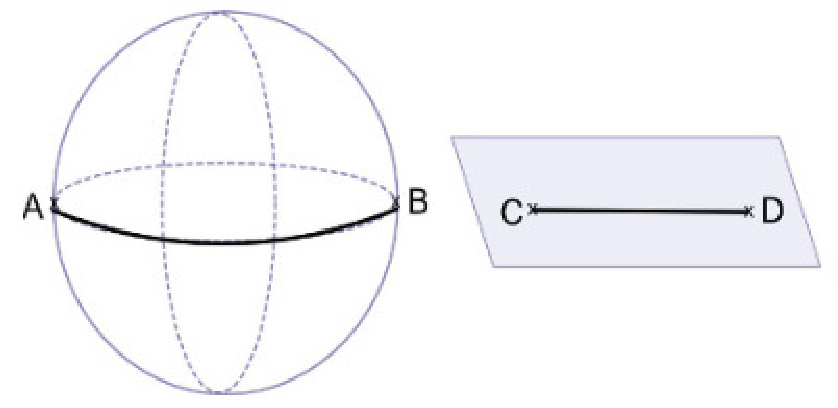
\includegraphics[scale=0.35]{fig12_1.pdf}
	\figcaption{弯曲空间与平直空间中的两点间距}
    \label{fig12.1}
}

现在就能“导出” Einstein 场方程了,因为能放在能动张量对面的量只有一个:Einstein张量$G_{\mu \nu}$。这是因为 Einstein 张量是度规$g_{\mu \nu}$及其一阶、二阶导数的函数中唯一\footnote{译注:至多差一常数与度规张量的乘积,即著名的宇宙学常数$Lambda$} 的无散度%
\mpar{即$\partial^\mu G_{\mu \nu} = 0$.}%
函数。不管其多复杂,放到等号一边描述曲率的量只能是它,因为
\begin{equation}
\label{equ12.3}
    T_{\mu \nu} = C G_{\mu \nu}, \quad \text{由} \partial^\mu T_{\mu \nu} = 0 \to \partial^\mu G_{\mu \nu} = 0.
\end{equation}
Einstein 张量是二阶张量%
\mpar{二阶张量是指它有两个指标$\mu \nu$,这与散度为零一样也是限制之一,因为$T_{\mu \nu}$是二阶张量。}%
,正好符合要求。

Einstein张量通过Ricci张量$R_{\mu \nu}$、Ricci标量$R$(即Ricci张量的迹:$R \equiv R^\nu_\nu$)和度规张量$g_{\mu \nu}$定义:
\begin{equation}
\label{equ12.4}
    G_{\mu \nu} = R_{\mu \nu} - \frac{1}{2} R g_{\mu \nu}.
\end{equation}
其中Ricci张量由Christoffel符号$\Gamma^\mu_{\nu \rho}$定义:
\begin{equation}
\label{equ12.5}
    R_{\alpha \beta} = \partial_\rho \Gamma^\rho_{\beta \alpha} - \partial_\beta \Gamma^\rho_{\rho \alpha} + \Gamma^\rho_{\rho \lambda} \Gamma^\lambda_{\beta \alpha} - \Gamma^\rho_{\beta \lambda} \Gamma^\lambda_{\rho \alpha}
\end{equation}
其中 Christoffel 符号通过度规张量定义:
\begin{equation}
\label{equ12.6}
    \Gamma^d_{ab} = \frac{1}{2} g^{cd} \left( \frac{\partial g_{ca}}{\partial x^b} + \frac{\partial g_{cb}}{\partial x^a} - \frac{\partial g_{ab}}{\partial x^c} \right) = \frac{1}{2} g^{cd} (\partial_b g_{ca} + \partial_a g_{cb} - \partial_c g_{ab}).
\end{equation}
上面的式子复杂得吓人,这稍微揭示了广义相对论计算的繁复程度。

现在考虑物体在弯曲时空中的行为。设自由物体经过弯曲时空中的$A, B$两点,物体在$A, B$之间的轨迹是怎样的?容易猜想物体沿弯曲时空中两点间的最短路径(称为短程线)运动,确实如此(证明略)。这样,给定质能分布$T_{\mu \nu}$之后就可根据Einstein场方程计算度规与Christoffel符号,从而得到自由质点的轨迹——{\bf 短程线方程(geodesic equation)}:
\begin{equation}
\label{equ12.7}
    \frac{d^2 x^\lambda}{dt^2} + \Gamma^\lambda_{\mu \nu} \frac{d x^\mu}{dt} \frac{d x^\nu}{dt} = 0.
\end{equation}
测地线是流形上的两点间局域最短%
\mpar{这一说法是过于简单的,正确的概念需要微分几何的相关知识,超出本书范围。}%
的连线。

有趣的是,Einstein将Christoffel符号视作引力场%
\mpar{一般将度规视为引力场。}%
:
\begin{quote}
若$\Gamma^\mu_{\nu \rho}$消失,则(自由)质点沿直线匀速运动,因此$\Gamma^\mu_{\nu \rho}$描述了关于匀速直线的偏离,它们是引力场的分量。
\end{quote}
\begin{flushright}
-- {\bf Albert Einstein}\mpar{Albert Einstein. The foundation of the general theory of relativity. 1916}
\end{flushright}
从\ref{equ12.7}式就能理解Einstein所说的,令$\Gamma^\mu_{\nu \rho} = 0$,测地线方程退化为:
\begin{equation}
\label{equ12.8}
    \frac{d^2 x^\lambda}{dt^2} = 0.
\end{equation}
方程的解是一条直线。

弯曲时空的另一有趣事实是微分符号的变化。平直时空中的导数利用下式定义:
\begin{equation}
\label{equ12.9}
    f'(a) = \lim_{h \to 0} \frac{f(a + h) - f(a)}{h}.
\end{equation}
上式用到了函数$f$在两个不同点的值。弯曲时空的情形不像平直时空那样简单。如图12.2,如果想比较球面上不同位置的两个向量的差值,怎样才能得到它们真正的差而除去弯曲空间造成的影响?微分几何告诉我们可以进行平移,将一个向量平移到另一个向量的位置,从而可以%
\mpar{实际上,微分几何中的坐标系都是局域的。\ref{sec3.11}节讲过,流形的主要特征是局域平直(像Euclidean空间)。因此,流形上对象的坐标只在一个坐标域内有效,同样只能在同一坐标域内比较不同对象的坐标差值。}%
比较它们。

\marginpar{
	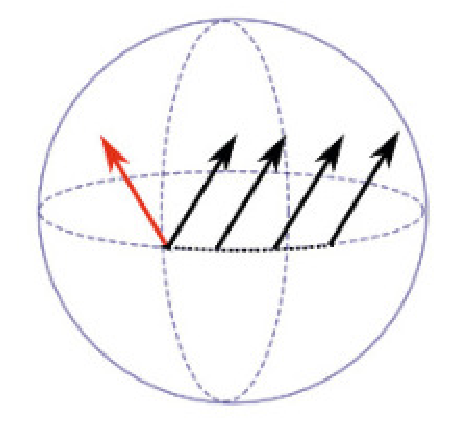
\includegraphics[scale=0.5]{fig12_2.pdf}
	\figcaption{为了比较红色箭头与黑色箭头,我们将黑色箭头平移到红色箭头的位置。}
}

弯曲空间中的导数称为{\bf 协变导数 (covariant derivative)}%
\mpar{这里的Christoffel符号$\Gamma^a_{\phantom{a}bc}$通常称为联络系数,因为它们联系了进行比较的两点。}%
:
\begin{equation}
\label{equ12.10}
    D_b v^a \equiv \partial_b v^a + \Gamma^a_{\phantom{a}bc} v^c.
\end{equation}
因此,弯曲时空中的方程需要将普通导数替换为协变导数:
\begin{equation}
\label{equ12.11}
    \partial_b \to D_b = \partial_b + \Gamma^a_{\phantom{a}bc}.
\end{equation}
这很眼熟。见\ref{equ7.18}式,我们在先前的章节中讲过,自旋$0$或自旋$\frac{1}{2}$场拉格朗日量的局域$\mathcal{U}(1)$不变性要求与自旋$1$的场有特定的耦合。这一耦合可以用下式描述:
\begin{equation}
\label{equ12.12}
    \partial_\mu \to D_\mu \equiv \partial_\mu + i \mathrm{e} A_\mu.
\end{equation}
注意这不只是个数学技巧,它导出了正确的电磁学理论。弱相互作用的情形也类似:
\begin{equation}
\label{equ12.13}
    \partial_\mu \to D_\mu \equiv \partial_\mu + i g \underbrace{W_\mu}_{\mathclap{= W_\mu^i \sigma^i}}.
\end{equation}
强相互作用也是:
\begin{equation}
\label{equ12.14}
    \partial_\mu \to D_\mu = \partial_\mu + i g' \underbrace{G_\mu}_{\mathclap{= T^C G^C_\mu}}.
\end{equation}
尽管上面各式的形式相似,但引力无法像其他相互作用那样量子化。其他相互作用都是用量子理论描述的,都给出概率性的实验预言。而广义相对论是经典理论,因为广相中的粒子沿确定的轨迹运动,没有概率性因素。

更糟糕的是目前没有任何实验能检测引力与其他力之间的相互作用。基本粒子间的引力太小,无法测量。因此忽视了引力,只考虑强、弱与电磁相互作用的标准模型就可以与实验符合得相当好。大质量物体的广义相对论效应实验上可以测量,但量子效应却十分微弱,因为大质量物体包含大量基本粒子,所有量子效应被平均掉了。第\ref{chap10}章导出了平均值的运动方程,它正是经典物理的形式,毫无量子效应。

引力的量子化的困难可以列出长长的列表,不过Einstein简明地论述了引力与其他相互作用的差异:
\begin{quote}
$\dots$ 根据广义相对论,引力与其他相互作用(特别是电磁力)相比地位特殊,因为描述引力场的十个方程\footnote{或许指Einstein场方程,代表十个方程。——译者}同时确定了时空的度量性质。
\end{quote}
\begin{flushright}
-- {\bf Albert Einstein}\mpar{Albert Einstein and Francis A. Davis.
{\it The Principle of Relativity}. Dover Publications, reprint edition, 6 1952. ISBN 9780486600819}
\end{flushright}

将普通导数替换为协变导数就能描述弯曲时空中的量子粒子,但这并非引力的动力学理论。Einstein场方程等号右侧(能动张量)容易量子化,选定合适的生成元就行了。困难的是等号左边的Einstein张量,它用Christoffel符号写为:
\begin{equation}
\label{equ12.15}
    G_{\alpha \beta} = (\delta^\gamma_\alpha \delta^\zeta_\beta - \frac{1}{2} g_{\alpha \beta} g^{\gamma \zeta}) (\partial_\varepsilon \Gamma^\varepsilon_{\gamma \zeta} - \partial_\zeta \Gamma^\varepsilon_{\gamma \varepsilon} + \Gamma^\varepsilon_{\varepsilon \sigma} \Gamma^\sigma_{\gamma \zeta} - \Gamma^\varepsilon_{\zeta \sigma} \Gamma^\sigma_{\varepsilon \gamma}).
\end{equation}
由此猜想Einstein场方程或许是$\Gamma^\varepsilon_{\zeta \sigma}$的场方程%
\mpar{就像Maxwell方程组与电磁场的关系那样。}%
,并且$\partial_b \to D_b = \partial_b + \Gamma^a_{\phantom{a} bc}$描述引力场$\Gamma^\varepsilon_{\zeta \sigma}$与其他场的耦合。

无论将度规张量(两个指标)还是Christoffel符号(三个指标)视为引力场,描述它们都需要Poincar\'e群的$(1, 1)$以及更高维的表示,或者说自旋$2, 3, \dots$表示。目前大多数物理学家认为引力场量子化后的引力子(graviton)是自旋为$2$的boson。

目前为止,没有靠谱的量子引力理论%
\mpar{许多尝试过程产生了无穷多个无穷大项,这对概率性预言来说十分要命。}%
能比下一节列出教科书上的标准引力理论给出进一步的信息。

\section*{Further Reading Tips \quad 阅读建议}
引力的标准理论——Einstein的广义相对论的更多信息可以参考以下文献:
\begin{itemize}
    \item {\bf  Ta-Pei Cheng - Relativity, Gravitation and Cosmology}%
    \mpar{Ta-Pei Cheng. {\it Relativity, Gravitation and Cosmology: A Basic Introduction.} Oxford University Press, 2nd edition, 1. 2010. ISBN 9780199573646}%
    是一本内容丰富、起点低的广义相对论入门教材,其中有大量启发性的论述。是快速入门的首选。
    \item {\bf  A. Zee - Einstein Gravity in a Nutshell}%
    \mpar{Anthony Zee. {\it Einstein Gravity in a Nutshell.} Princeton University Press, 1st edition, 5. 2013. ISBN 9780691145587}%
    是广义相对论的最佳教材。此书从基本概念开始,避免不必要而复杂的数学概念,精彩地解释了广义相对论的起源与应用。
    \item {\bf  Charles W. Misner, Kip S. Thorne, John Archibald Wheeler - Gravitation}%
    \mpar{ Charles W. Misner, Kip S. Thorne, and John Archibald Wheeler. {\it Gravitation.} W.H. Freeman, 1st edition, 9. 1973. ISBN 9780716703440}%
    是一本关于引力的鸿篇巨著,其中阐明了有大量其他教材未深入讨论的问题。
\end{itemize}
关于尝试引力量子化的更多信息可见
\begin{itemize}
    \item {\bf John C. Baez, Javier P. Muniain - Gauge Fields, Knots, and Gravity}%
    \mpar{ John C. Baez and Javier P. Muniain. {\it Gauge Fields, Knots, and Gravity.} World Scientific Pub Co Inc, 1st edition, 9. 1994. ISBN 9789810220341}%
    以面向物理学家的方式介绍了引力量子化的数学工具。
\end{itemize}

\input{./Chaps/Chap13}

%!TEX root = main.tex
%!TEX encoding = UTF-8 Unicode

\appendix

\part{Appendix 附录}
\chapter[矢量代数]{Vector calculus 矢量代数}\label{appendix.A}
物理中常用三个数$ \begin{pmatrix}
x \\ y \\ z
\end{pmatrix}$来描述一个东西的位置。我们将其称作矢量$\vec{v}$,在它头上放了一个箭头。这三个数称作矢量沿三个坐标轴的分量。第一个数说了这个矢量沿$x$方向走了多远,第二个是沿$y$方向以及第三个是沿$z$方向。例如,$\vec{w}= \begin{pmatrix}
0 \\ 4 \\ 0
\end{pmatrix}$是一个指向$y$轴方向的矢量。

\marginpar{
	\includegraphics[width=.4\textwidth]{fig_appendix_A_1.png}
}

矢量间可以相加
\begin{equation}
\vec{v} = \begin{pmatrix}
v_x \\ v_y \\ v_z
\end{pmatrix} \quad
\vec{w} = \begin{pmatrix}
w_x \\ w_y \\ w_z
\end{pmatrix} \quad \rightarrow \quad
\vec{v}+\vec{w}= \begin{pmatrix}
v_x+w_x \\ v_y+w_y \\ v_z+w_z
\end{pmatrix}
\end{equation}
也可以相乘
\begin{equation}
\vec{v}\cdot\vec{w} = \begin{pmatrix}
v_x \\ v_y \\ v_z
\end{pmatrix} \cdot \begin{pmatrix}
w_x \\ w_y \\ w_z
\end{pmatrix} =
v_xw_x +v_yw_y +v_zw_z\text{。}
\end{equation}

乘法的结果是一个数($=$标量)而不是矢量,其有特定的名称:{标量积(scalar product)}。计算矢量与自身的标量积可以得到其长度:
\begin{equation}
\text{长度}(\vec{v}) = \sqrt{\vec{v}\cdot\vec{v}}\text{。}
\end{equation}
注意并不是随便三个量都可以写在一起,用括号包起来,作为一个矢量。例如,把一个房间里的温度$T$,压强$P$和湿度$H$放在一起:
\begin{equation}
\begin{pmatrix}
T \\ P \\ H
\end{pmatrix}\text{。}
\end{equation}
没人阻止我们把他们放在一起,但这结果毫无意义,而且显然不是一个矢量,因为不存在能将它们混在一起的线性关系。而如果我们仅仅是换一个视角\footnote{译注:本意,即视线的角度。}去考察一个矢量,它的坐标分量将会互相转换%
\mpar{这一点等会儿会有更清楚的说明。}%
。故将这些坐标分量写在一起用括号包起来是有用的。另外,如果分量会因视角的改变而发生混合的话,将其写成位置矢量的形式是有用的。

从现在开始,我们将完全按照位置矢量$\vec{v}$的变换方式的量称为一个矢量。这句话的意思是,如果在某种变换下我们有$\vec{v}\rightarrow\vec{v}'=M\vec{v}$,则任何依$\vec{w}\rightarrow\vec{w}'=M\vec{w}$作变换的量都是矢量。动量和加速度是典型的例子。

物理中我们将经常碰到这种思路。当我们把一些量写在一起放在一对括号中时,它们未必是矢量,但一定是在某些线性算符下相互变换的量。线性算符常通过与矩阵的乘法来表示。

\section[基矢]{Basis Vectors 基矢}\label{appendix.A.1}
我们可以通过引入基矢来更一般的讨论沿坐标轴的分量这件事。基矢是一组线性独立%
\mpar{一组矢量$\{\vec{a},\vec{b},\vec{c}\}$被称为是线性独立的,若方程$c_1\vec{a}+c_2\vec{b}+c_3\vec{c}=0$成立当且仅当$c_1=c_2=c_3=0$。这说的其实就是其中任何一个矢量不能表达为其他矢量的线性组合:如果有$c_1\vec{a}+c_2\vec{b}+c_3\vec{c}=0$对非零的系数成立,则有$c_1\vec{a}+c_2\vec{b}=-c_3\vec{c}$。}%
且长度为一%
\footnote{译注:一般资料上并不要求最后一条;满足这一条的称为单位基矢。}%
的矢量。三维里我们需要三个基矢,从而能将任何矢量都用基矢量的组合来表达。一个简单的选择是:
\begin{equation}
\vec{e}_1 = \begin{pmatrix}
1 \\ 0 \\ 0
\end{pmatrix}\text{,}\quad
\vec{e}_2 = \begin{pmatrix}
0 \\ 1 \\ 0
\end{pmatrix} \text{,}\quad
\vec{e}_3 = \begin{pmatrix}
0 \\ 0 \\ 1
\end{pmatrix}
\end{equation}
这样任意三维矢量$\vec{v}$都能用基矢表出
\begin{equation}
\vec{v} = \begin{pmatrix}
v_x \\ v_y \\ v_z
\end{pmatrix} = v_1\vec{e}_1 + v_2\vec{e}_2 + v_3\vec{e}_3 =
v_1 \begin{pmatrix}
1 \\ 0 \\ 0
\end{pmatrix}+
v_2  \begin{pmatrix}
0 \\ 1 \\ 0
\end{pmatrix} +
v_3  \begin{pmatrix}
0 \\ 0 \\ 1
\end{pmatrix}\text{。}
\end{equation}
$v_1,v_2,v_3$三个数叫做$\vec{v}$的分量。注意分量是依赖于基矢的。

前面提到的矢量\mpar{$\vec{w}= \begin{pmatrix}
0\\4\\0
\end{pmatrix}$}$\vec{w}$由此可以写成$\vec{w}= 0\vec{e}_1 + 4\vec{e}_2 + 0\vec{e}_3$。对基矢另一个同样好的选法是
\begin{equation}
\tilde\vec{e}_1 = \frac{1}{\sqrt{2}} \begin{pmatrix}
1 \\ 1 \\ 0
\end{pmatrix}\text{,}\quad
\tilde\vec{e}_2 = \frac{1}{\sqrt{2}} \begin{pmatrix}
1 \\ -1 \\ 0
\end{pmatrix} \text{,}\quad
\tilde\vec{e}_3 = \begin{pmatrix}
0 \\ 0 \\ 1
\end{pmatrix}\text{。}
\end{equation}
在这组基下矢量$\vec{w}$看起来会有点不同:
\begin{equation}
\vec{w}= 2\sqrt{2}\tilde\vec{e}_1 -2\sqrt{2}\tilde\vec{e}_2 + 0\tilde\vec{e}_3
= 2\sqrt{2} \frac{1}{\sqrt{2}} \begin{pmatrix}
1 \\ 1 \\ 0
\end{pmatrix}-2\sqrt{2}
\frac{1}{\sqrt{2}} \begin{pmatrix}
1 \\ -1 \\ 0
\end{pmatrix} =\begin{pmatrix}
0\\4\\0
\end{pmatrix} \text{。}
\end{equation}
从而将$\vec{w}$用在新基矢下的分量写出
\[
\tilde\vec{w} = \begin{pmatrix}
2\sqrt{2} \\ -2\sqrt{2} \\ 0
\end{pmatrix}\text{。}
\]
这并不是一个不同的矢量,而只是一个不同的描述!准确地讲,$\tilde\vec{w}$是原坐标系中的矢量$\tilde\vec{w}$在一个相对有旋转的坐标系下描述。%
\footnote{译注:在整个附录\ref{appendix.A}里作者就没说过几句准确的话,这句话也说得挺糙的。}

\section[坐标系变换]{Change of Coordinate Systems 坐标系变换}\label{appendix.A.2}
通过矩阵,我们可以更精确地描述不同坐标系间的联系。两个不同的坐标系可以代表实验中两个持不同视角的观察者,或者仅仅是{\bf 一个}想使用一套新的基矢的观察者。这些描述之间的关系是什么?为了避免复杂的讨论,让我们假定这两个坐标系的原点和$z$轴都是一样的。这样的话就只是$x$和$y$轴有区别了。进一步假定实验中某个重要的量用矢量$\vec{v}$描述。

如果第一个观察者看到的是矢量$\vec{v}= \begin{pmatrix}
v_x \\ v_y \\ v_z
\end{pmatrix}$,我们能通过三角函数$\sin(\phi)$,$\cos(\phi)$和$\tan(\phi)=\frac{\sin(\phi)}{\cos(\phi)}$来计算出第二个观察者看到的$\vec{v}= \begin{pmatrix}
v_{x'} \\ v_{y'} \\ v_{z'}
\end{pmatrix}$,如图\ref{fig:appendix.A.1} 所示:
\picmpar{
	\includegraphics[width=\textwidth]{fig_appendix_A_3.png}
	\caption{矢量在两个不同的坐标系下分量的示意图。细节见正文。}
	\label{fig:appendix.A.1}
}

计算$v_x$和$v_{x'}$的关系,由
\[
\cos(\phi)=\frac{v_{x'}}{v_x+a} \rightarrow v_{x'}=(v_x+a)\cos(\phi)
\]
以及
\[
\tan(\phi)=\frac{a}{v_y}\rightarrow a=v_y\tan(\phi)\text{。}
\]
得到
\[
\begin{aligned}
v_{x'}=(v_x+v_y\tan(\phi))\cos(\phi)&=\left(v_x+v_y\frac{\sin(\phi)}{\cos(\phi)}\right)\cos(\phi) \\
 & = v_x\cos(\phi)+v_y\sin(\phi)\text{。}
\end{aligned}
\]
类似的,利用
\[
\cos(\phi) = \frac{v_y}{v_{y'}+b}\rightarrow v_{y'}=v_y\frac{1}{\cos(\phi)}-b
\]
和
\[
\tan(\phi)=\frac{v_y}{v_{y'}+b}\rightarrow b=v_{x'}\tan(\phi)
\]
再借助$\sin^2(\phi)+\cos^2(\phi)=1$导出
\[\begin{split}
v_{y'}&=v_y\frac{1}{\cos(\phi)}-v_{x'}\tan(\phi)=v_y\frac{1}{\cos(\phi)}-(v_x\cos(\phi)+v_y\sin(\phi))\frac{\sin(\phi)}{\cos(\phi)}  \\
&= v_y\frac{\sin^2(\phi)+\cos^2(\phi)}{\cos(\phi)}-v_x\sin(\phi)-v_y\frac{\sin^2(\phi)}{\cos(\phi)} = v_y\cos(\phi)-v_x\sin(\phi)
\end{split}\]
最终有$v_{y'}=-v_x\sin(\phi)+v_y\cos(\phi)$。

我们能将其用一个旋转矩阵来表达:
\begin{equation}
\begin{aligned}
\begin{pmatrix}
v_{x'} \\ v_{y'} \\ v_{z'}
\end{pmatrix} &= R_z(\phi)\vec{v} =
\begin{pmatrix}
\cos(\phi) & \sin(\phi) & 0 \\
-\sin(\phi) & \cos(\phi) & 0 \\
0 & 0 & 1
\end{pmatrix}
\begin{pmatrix}
v_x \\ v_y \\ v_z
\end{pmatrix} \\
&= \begin{pmatrix}
\cos(\phi)v_x+\sin(\phi)v_y \\ -\sin(\phi)v_x+\cos(\phi)v_y \\ v_z
\end{pmatrix}\text{。}
\end{aligned}
\end{equation}
将矩阵的每一行与未旋转的矢量相乘,便得到了旋转后的矢量。如之前所提到的,沿$z$轴的分量$v_3$对于不同的观察者而言是相同的。矩阵$R_z(\phi)$描述了一个绕$z$轴转动了角度$\phi$的旋转。

\section[矩阵乘法]{Matrix Multiplication 矩阵乘法}\label{appendix.A.3}
像这样通过矩阵来作计算是一个极大的简化。矩阵乘法的规则就是行乘列。如果将一个矢量看做一个一列三行的矩阵(一个$3\times 1$矩阵),则标量积也可以看做是矩阵乘法的一种特殊情况。即
\begin{equation}
\vec{v}\cdot\vec{w} = \vec{v}^T\vec{w}= \begin{pmatrix}
v_x & v_y & v_z
\end{pmatrix} \begin{pmatrix}
w_x \\ w_y \\ w_z
\end{pmatrix} = v_xw_x +v_yw_y +v_zw_z\text{,}
\end{equation}
其中$T$代表转置,即行变成列,列变成行。那么$\vec{v}^T$便是一个$1$行$3$列的矩阵。这样写的话标量积就也成了行乘列的矩阵乘法。

类似的,两个矩阵的乘法也就是左边矩阵的每一行乘右边矩阵的每一列,如图\ref{fig:appendix.A.2}。下面是一个具体的例子

\picmpar{
	\includegraphics[width=.4\textwidth]{fig_appendix_A_4.png}
	\caption{矩阵乘法示意图。时时刻刻记住{\bf 行乘列}。第一个指标代表所在的行数,第二个代表列数。在例子中,乘积矩阵红色的元素$c_{1,2}=a_{1,1}b_{1,2}+a_{1,2}b_{2,2}$,蓝色的元素$c_{3,3}=a_{3,1}b_{1,3}+a_{3,2}b_{2,3}$。一般的,$c_{i,j}=a_{i,k}b_{k,j}=a_{i,1}b_{1,j}+a_{i,2}b_{2,j}+\dots$ Figure by Olivier Perrin (Bilou Wikimedia Commons) released under a CC BY-SA 3.0 licence: \url{http://creativecommons.org/licenses/by-sa/3.0/deed.en}. URL: \url{http://commons.wikimedia.org/wiki/File:Matrix_multiplication_diagram_2.svg}, Accessed: 28.1.2015}
	\label{fig:appendix.A.2}
}

\begin{equation}
\begin{aligned}
M= \begin{pmatrix}
2 & 3 \\ 1 & 0
\end{pmatrix} \quad N =
\begin{pmatrix}
0 & 1 \\ 4 & 8
\end{pmatrix} \\
MN = \begin{pmatrix}
2 & 3 \\ 1 & 0
\end{pmatrix}
\begin{pmatrix}
0 & 1 \\ 4 & 8
\end{pmatrix} =
\begin{pmatrix}
2\cdot 0+3\cdot 4 & 2\cdot 1+3\cdot 8 \\ 1\cdot 0+0\cdot 4 & 1\cdot 1+0\cdot 8
\end{pmatrix} =
\begin{pmatrix}
12 & 26 \\ 0 & 1
\end{pmatrix}
\end{aligned}
\end{equation}
时刻把{\bf 行乘列}记在脑子里\footnote{译注:说起来,什么是行什么是列也是一个需要记牢的东西,尤其是与台湾友人交流时。}。注意两个矩阵的乘法是不对易的,即一般来说$MN\ne NM$。

\section[标量]{Scalars 标量}\label{appendix.A.4}
另一个值得注意的事情是,两个矢量标量积的结果对于所有观察者而言都是相同的。这看起来可以作为标量的定义:标量是对于全部观察者都相同的量。这不只是简单的在说每一个数都是标量,因为矢量的每一个分量都是一个数,但是它们对于不同的观察者而言却不一样。作为对比,两个矢量的标量积对于全体观察者却是相同的。这源于,矢量的长度与其与自身的标量积直接相关这一事实。改变观察的视角或位置并不会改变任何东西的长度。矢量的长度被称作旋转下的不变量,即无论我们怎样旋转系统其都保持原样。

\section[左手/右手坐标系]{Right-handed and Left-handed Coordinate Systems 左手/右手坐标系}\label{appendix.A.5}
当我们谈论两个观察者时,我们默认了它们对坐标系的定义都是相同的。而事实上,我们有两种可能的选择,它们这是依旧能通过矩阵乘法相联系,却不能靠转动了。两个观察者可能是一个选择了所谓的右手坐标系,而另一个选择了左手坐标系。

\picmpar{
	\includegraphics[width=.4\textwidth]{fig_appendix_A_5.png}
	\caption{右手坐标系和左手坐标系。 Figure by Primalshell (Wikimedia Commons) released under a CC-BY-SA-3.0 licence: \url{http://creativecommons.org/licenses/by-sa/3.0/deed.en}. URL:\url{http://commons.wikimedia.org/wiki/File:3D_Cartesian_Coodinate_Handedness.jpg}, Accessed: 1.12.2014}
}

我们无法将一个左手系旋转成一个右手系。事实上,这两类坐标系通过镜面反射相关联。这就是说,右手系和左手系由如下形式的变换相联系%
\footnote{译注:原文这里给出的其实是一个相对原点的反射,而不是镜面反射。当然,这两种反射之间只差一个转动。}
\begin{equation}
\begin{pmatrix}
v_1 \\ v_2 \\ v_3
\end{pmatrix} \rightarrow
\begin{pmatrix}
-v_1 \\ -v_2 \\ -v_3
\end{pmatrix}\text{,}
\end{equation}
就是说把全部空间坐标都反一个号。人们也习惯于将这类变换称作{\bf 宇称变换(parity transformation)}。我们可以用如下方式来表示一个宇称变换
\begin{equation}
\vec{v} \rightarrow \vec{v}' = P\vec{v} = \begin{pmatrix}
-1 & 0 & 0 \\ 0 & -1 & 0 \\ 0 & 0 & -1
\end{pmatrix}
\begin{pmatrix}
v_1 \\ v_2 \\ v_3
\end{pmatrix} =
\begin{pmatrix}
-v_1 \\ -v_2 \\ -v_3
\end{pmatrix}\text{。}
\end{equation}

\chapter[微积分]{Calulus 微积分}\label{appendix.B}

\section[Product Rule]{Product Rule 莱布尼兹律}\label{appendix.B.1}
莱布尼兹律\footnote{译注:直译为“乘积规则”,鉴于这种叫法在中文文本中较罕见,故译作“莱布尼兹律”。}
\begin{equation}
\frac{\rd}{\rd x} \left(f(x)g(x)\right) = \left(\frac{\rd f(x)}{\rd x}\right) g(x) + f(x) \left(\frac{\rd g(x)}{\rd x}\right) \equiv f'g + fg'
\label{equB.1}
\end{equation}
可直接由导数的定义得到
\begin{equation*}
\begin{aligned}
\frac{\rd}{\rd x} \left[f(x)g(x)\right] &= \lim_{h\rightarrow 0} \frac{f(x+h)g(x+h)-f(x)g(x)}{h} \\
 &= \lim_{h\rightarrow 0} \frac{\left[f(x+h)g(x+h)-f(x+h)g(x)\right]+\left[f(x+h)g(x)-f(x)g(x)\right]}{h} \\
 &= \lim_{h\rightarrow 0}{f(x+h)\frac{g(x+h)-g(x)}{h} +g(x)\frac{f(x+h)-f(x)}{h}} \\
 &= f(x)g'(x)+g(x)f'(x)
\end{aligned}
\end{equation*}
\section[分部积分]{Integration by Parts 分部积分}\label{appendix.B.2}
\begin{quote}
据说, Peter Lax 被授予美国国家科学奖章时,其他获奖人(可能不是数学家)问他凭借什么拿到的这个奖。 Lax 回答:“我做了个分部积分。” 
\begin{flushright}
	--- Willie Wrong\mpar{是他在\url{www.math.stackexchange.com}上说的。}
\end{flushright}
\end{quote}

从莱布尼兹律可以直接得到一个重要的积分手段。将莱布尼兹律一式积分%
\mpar{见\eqref{equB.1}式,并利用微积分基本定理$\int_a^b h'(x)=h(b)-h(a)$。}
\begin{equation}
\underbrace{\int_a^b \rd x\, \frac{\rd}{\rd x}\left(f(x)g(x)\right)}_{=\left.f(x)g(x)\right|_a^b} = \int_a^b\rd x\, \left(\frac{\rd f(x)}{\rd x}\right)g(x) + \int_a^b\rd x\, f(x)\left(\frac{\rd g(x)}{\rd x}\right)
\end{equation}
移项,得到
\begin{equation}
\int_a^b \rd x\, \left(\frac{\rd f(x)}{\rd x}\right)g(x) = \left.f(x)g(x)\right|_a^b - \int_a^b\rd x\, f(x)\left(\frac{\rd g(x)}{\rd x}\right)\text{。}
\label{equB.3}
\end{equation}
当讨论场的物理时,这个手段很是有用:在全空间作积分时,即$a=-\infty,b=\infty$,由于一切场量在无穷远处都必须为零%
\mpar{\ref{sec2.4}节中我们说到了没什么能比光速还快,故无穷远处的场一定不会对有限$x$处的物理产生影响。}%
,边界项为零$\left.f(x)g(x)\right|_a^b=0$。

\section[Taylor 级数]{The Taylor Series\quad Taylor 级数}\label{appendix.B.3}
Taylor 级数使我们能将任何无穷阶可微函数写成幂级数形式
\begin{equation}
f(x) = f(a) + (x-a)f'(a) + \frac{1}{2}(x-a)^2f''(a)+\dots
\end{equation}
\begin{itemize}
\item 一方面我们能用它来求某些函数的级数形式。这可以用来,例如,说明$\ue^{\ri x}=\cos (x)+\ri\sin (x)$。
\item 另一方面,也能用它来得到函数在某点附近的近似值。当出于某些原因我们可以略去高阶项,不用考虑无穷多项时,这公式的用处会很大。比如说我们要算函数$f(x)$在$y$的邻域中一点$y+\Delta y$的值,可以写出%
\mpar{不要被这些变量的名字搞混了。上面的公式里我们是从$a$出发计算函数在$x$处的值。而这里我们是希望利用$y$处的信息来得到$f$在$y+\Delta y$处的性质。准确的关系是:$x=y+\Delta y$和$a=y$。}
\end{itemize}
\begin{equation}
f(y+\Delta y) = f(y)+(y+\Delta y-y)f'(y)+\dots =f(y)+\Delta y f'(y)+\dots
\end{equation}
这就是说,通过在$y$处函数的性质,我们能得到其在$y+\Delta y$处的近似值。对于无穷小邻域%
\footnote{译注:原文有误,已更正。}%
$\Delta y=\epsilon\rightarrow 0$的极端情况,函数的改变量可以仅用 Taylor 级数的一(线性)项来表示
\begin{equation}
\Delta f =f(y+\epsilon)-f(y)=f(y)+\epsilon f'(y)+\dots -f(y)=\epsilon f'(y) + \underbrace{\dots}_{\mathclap{\approx 0\text{由于}\epsilon^2\approx 0}}
\end{equation}

这个式子是最有用的数学工具之一,它也能通过微积分基本定理和分部积分推出来。基本定理说
\begin{equation}
\int_a^x\rd t\, f'(t) = f(x) - f(a) \rightarrow f(x)=f(a)+\int_a^x\rd t\, f'(t)\text{。}
\end{equation}
可以将第二项用分部积分写开:在$f'(t)$前面补一个$1$成$1f'(t)$,利用\eqref{equB.3}式取$g'(t)=1$的情况。分部积分能改写积分%
\mpar{译注:原文有误,已更正。}%
$\int_a^b v'u = \left.vu\right|_a^b-\int_a^b vu'$,积掉一项而对另一项微分。这里我们积$g'(t)=1$而微分$f'(t)$,即式子里$g'=v'$及$f'=u$。求得
\begin{equation}
f(x) = f(a)+\int_a^x\rd t\, f'(t) = f(a) + \left.g(t)f(t)\right|_a^x - \int_a^b \rd t g(t)f''(t) \text{。}
\end{equation}

现在的问题是$g(t)$是啥。我们目前只知道$g'(t)=1$,但却有无穷多个函数的导数都是这个:对于任意常数$c$,函数$g=t+c$都满足$g'(t)=1$。我们选取%
\mpar{方程对任意$c$都成立,我们自然可以随便选一个,但那样就推不出我们想要的公式了。选取恰当的$c$是为了得到一个有用的关于$f(x)$的公式。否则$f(x)$将会同时出现在等式两侧。}%
$g=t-x$,即将积分上界的负值$-x$作为我们的常数$c$。从而上式的第二项就可以写作
\begin{equation}
\left.g(t)f(t)\right|_a^x = \left.(t-x)f(t)\right|_a^x = \underbrace{(x-x)}_{=0}f(x) -(a-x)f(a) =(x-a)f(a)
\end{equation}
从而整个式子现在写作
\begin{equation}
f(x) = f(a) + (x-a)f'(a)+\int_a^x\rd t\, (x-t)f''(t)\text{。}
\end{equation}
对最后一项再次使用分部积分,现在是%
\mpar{注意$v='(x-t)$对$t$的积分会出一个符号:$v=-(x-t)^2+d$积分常数$d$取作零。}
$v'=(x-t)$和$u=f''(t)$:
\begin{equation*}
\rightarrow \int_a^x \rd t\, \underbrace{(x-t)}_{\mathclap{=v'}}\underbrace{f''(t)}_{=u} = \left.\underbrace{-\frac{1}{2}(x-t)^2}_{=v} \underbrace{f''(t)}_{=u}\right|_a^x - \int_a^x \rd t\, \underbrace{\left(-\frac{1}{2}(x-t)^2\right)}_{=v}\underbrace{f'''(t)}_{=u'}
\end{equation*}
边界项同样简单的是零
\begin{equation*}
\left.-\frac{1}{2}(x-t)^2f''(t)\right|_a^x = -\frac{1}{2}\underbrace{(x-x)^2}_{=0}f''(x) + \frac{1}{2}(x-a)^2f''(a)\text{。}
\end{equation*}
得到公式
\begin{equation}
f(x)=f(a)+(x-a)f'(a)+\frac{1}{2}(x-a)^2f''(a)+\int_a^x \rd t\, \frac{1}{2}(x-t)^2 f'''(t)\text{。}
\end{equation}
可以继续将最后一项分部积分,但是我们应该能直接肉眼观察出规律了。Taylor 级数可以利用求和号$\Sigma$写成更紧凑的形式:
\begin{equation}
\begin{aligned}
f(x) =& \sum_{n=0}^\infty\frac{f^{(n)}(a)(x-a)^n}{n!} \\
 =& \frac{f^{(0)}(a)(x-a)}{0!} + \frac{f^(1)(a)(x-a)^1}{1!} + \frac{f^{(2)}(a)(x-a)^2}{2!} \\
 =& \frac{f^{(3)}(a)(x-a)^3}{3!}+\dots \text{,}
\end{aligned}
\label{equ.appendix.B.12}
\end{equation}
其中$f^{(n)}$代表$f$的$n$阶导数,例如$f^{(2)}=f''$,$n!$代表$n$的阶乘,即$n!=1\cdot 2\cdot 3\dots n$。比如对$n=5$有$5!=5\cdot 4\cdot 3\cdot 2\cdot 1=120$,$2!=2\cdot 1=2$,以及定义$0!=1$。级数是下一节的主题。
\section[级数]{Series 级数}\label{appendix.B.4}
上一节中我们碰巧发现了含有无穷求和的一个重要等式。在这一节里将介绍关于求和的一些小技巧和几个重要级数。
\subsection[几个重要的级数]{Important Series 几个重要的级数}\label{appendix.B.4.1}
从上一节中我们学到了任意无穷可微的函数都可以写成级数的形式%
\footnote{译注:一个典型的反例是$f(x)=\exp(-1/x^2)$,它在原点处(补充定义后)任意阶导数都为零。}%
。让我们从最重要的例子开始:指数函数$\ue^{x}$。它的泰勒展开式可以直接写出:
\begin{equation}
\ue^x  = \sum\limits_{n=0}^{\infty} \frac{x^n}{n!} \text{,}
\end{equation}
用到了指数函数的%
\footnote{译注:某一种}
定义,导函数等于自身:$(\ue^x)'=\ue^x$。将$a=0$带入 Taylor 级数,利用$\ue^0=1$,便得到指数函数的 Taylor 级数(\eqref{equ.appendix.B.12}式):
\begin{equation}
\ue^x = \sum\limits_{n=0}^\infty \frac{\ue^0(x-0)^n}{n!} = \sum\limits_{n=0}^\infty \frac{x^n}{n!}
\end{equation}

这个级数也可以作为$\ue^x$的定义式。

另外两个无穷可微的重要函数是$\sin(x)$和$\cos(x)$。利用$(\sin(x))'=\cos(x)$,$(\cos(x))'=-\sin(x)$,$\cos(0)=1$以及$\sin(0)=0$,可以推得它们的泰勒级数。
\begin{equation*}
\sin(x) = \sum\limits_{n=0}^\infty \frac{\sin^{(n)}(0)(x-0)^n}{n!}\text{。}
\end{equation*}
由于$\sin(0)=0$,故全部偶数$n$项都为零,由此可以将求和分开:注意到
\begin{equation}
\begin{aligned}
\sum_{n=0}^{\infty}n &= \sum_{n=0}^\infty (2n+1) + \sum_{n=0}^\infty (2n) \\
1+2+3+4+5+6\dots &= 1+3+5\dots + 2+4+6+\dots
\end{aligned}
\end{equation}
将$\sin(x)$的求和分裂开来
\begin{equation}
\begin{aligned}
\sin(x) &= \sum\limits_{n=0}^\infty \frac{\sin^{(2n+1)}(0)(x-0)^{2n+1}}{(2n+1)!}+ \underbrace{\sum\limits_{n=0}^\infty \frac{\sin^{(2n)}(0)(x-0)^{2n}}{(2n)!}}_{=0} \\
 &= \sum\limits_{n=0}^\infty \frac{\sin^{(2n+1)}(0)(x-0)^{2n+1}}{(2n+1)!}\text{。}
\end{aligned}
\label{equ.appendix.B.16}
\end{equation}
$\sin(x)$的全部偶数阶导数,$\sin^{(2n)}$也是$\sin(x)$(除去可能有的负号),由于$\sin(0)=0$所以说第二项为零。$\sin(x)$全部奇数阶导数是$\cos(x)$,除去可能的负号。我们有
\begin{equation}
\begin{aligned}
\sin(x)^{(1)}&=\cos(x) \\
\sin(x)^{(2)}&=\cos'(x)=-\sin(x) \\
\sin(x)^{(3)}&=-\sin'(x)=-\cos(x) \\
\sin(x)^{(4)}&=-\cos'(x)=\sin(x) \\
\sin(x)^{(5)}&=\sin'(x)=\cos(x) \\
\end{aligned}
\end{equation}
规律是$\sin^{(2n+1)}(x)=(-1)^n\cos(x)$,你可以将任意整数$n$带入验证%
\mpar{\begin{align}
\sin(x)^{(1)}=&\sin(x)^{(2\cdot 0+1)}\nonumber \\
&=(-1)^0\cos(x)\nonumber \\
&=\cos(x),\sin(x)^{(3)}\nonumber \\
&=\sin(x)^{(2\cdot 1+1)}\nonumber \\
&=(-1)^1\cos(x)\nonumber \\
&=-\cos(x)\nonumber
\end{align}}%
。由此将\eqref{equ.appendix.B.16}式改写作
\begin{equation}
\begin{aligned}
\sin(x) &= \sum\limits_{n=0}^{\infty}\frac{\sin^{(2n+1)}(0)(x-0)^{2n+1}}{(2n+1)!} \\
&= \sum\limits_{n=0}^{\infty}\frac{(-1)^n\cos(0)(x-0)^{2n+1}}{(2n+1)!} \\
&\underbrace{=}_{\cos(0)=1} \sum\limits_{n=0}^\infty \frac{(-1)^n(x)^{2n+1}}{(2n+1)!}
\end{aligned}
\label{equ.appendix.B.18}
\end{equation}
这就是$\sin(x)$的 Taylor 级数,也可以作为$\sin(x)$的定义式。类似的,我们可以得到
\begin{equation}
\cos(x)= \sum\limits_{n=0}^{\infty}\frac{(-1)^n(x)^{2n}}{(2n)!}\text{,}
\label{equ.appendix.B.19}
\end{equation}
其奇数阶导数都正比于$\sin(0)=0$。

\subsection[分裂求和]{Splitting Sums 分裂求和}\label{appendix.B.4.2}
上一节中我们提到了一个有用的计算技巧。那儿我们用了下面这个例子
\begin{equation}
\begin{aligned}
\sum\limits_{n=0}^{\infty}n &= \sum\limits_{n=0}^\infty (2n+1) + \sum\limits_{n=0}^\infty (2n) \\
1+2+3+4+5+6\dots &= 1+3+5\dots + 2+4+6+\dots
\end{aligned}
\end{equation}
来表明我们可以将任何求和分解成偶数和奇数项。$2n$总是偶数,而$2n+1$总是奇数。在上一节中我们就看到了这很有用,但现在可以再看看另一个例子。如果将带有复变量$\ri x$的指数函数的级数分裂开来会怎样?
\begin{equation}
\begin{aligned}
\ue^{\ri x}= &\sum\limits_{n=0}^\infty \frac{(\ri x)^n}{n!}\\
 =& \sum\limits_{n=0}^\infty \frac{(\ri x)^{2n}}{(2n)!}+\sum\limits_{n=0}^\infty \frac{(\ri x)^{2n+1}}{(2n+1)!}
\end{aligned}
\end{equation}
用$(\ri x)^{2n}=\ri^{2n}x^{2n}$和$\ri^{2n}=(\ri^2)^n=(-1)^n$来写开。另外也需要$\ri^{2n+1}=\ri\cdot \ri^{2n}=\ri(-1)^n$。由此有
\begin{equation}
\begin{aligned}
\ue^{\ri x}= &\sum\limits_{n=0}^\infty \frac{(\ri x)^n}{n!}\\
 =& \sum\limits_{n=0}^\infty \frac{(-1)^n(x)^{2n}}{(2n)!}+\ri\sum\limits_{n=0}^\infty \frac{(-1)^n(x)^{2n+1}}{(2n+1)!}\\
 =& \underbrace{\sum\limits_{n=0}^\infty \frac{(-1)^n(x)^{2n}}{(2n)!}}_{=\cos(x)\text{ 见\eqref{equ.appendix.B.19}式}}+\ri\underbrace{\sum\limits_{n=0}^\infty \frac{(-1)^n(x)^{2n+1}}{(2n+1)!}}_{=\sin(x)\text{ 见\eqref{equ.appendix.B.18}式}}\\
 =& \cos(x)+\ri\sin(x)
\end{aligned}
\end{equation}

\subsection[Einstein 求和约定]{Einstein's Sum Convention\quad Einstein 求和约定}\label{appendix.B.4.3}
物理中经常有求和,老是写大大的求和号$\Sigma$是很烦人的一件事。所以说某个聪明人引入了一个约定,叫 Einstein 求和约定。根据这个约定每当一个指标在某些项中重复出现两次,如同上面的$n$,那么就意味着一个隐藏的求和号。即
\begin{equation}
a_na_n \equiv \sum\limits_n a_nb_n \text{。}
\end{equation}
其他形式的例子
\begin{equation}
a_nb_nc_m \equiv \sum\limits_n a_nb_nc_m \text{。}
\end{equation}
\begin{equation}
a_mb_nc_m \equiv \sum\limits_m a_mb_nc_m \text{。}
\end{equation}
但是
\begin{equation}
a_nb_m \ne \sum\limits_n a_nb_m\text{,}
\end{equation}
因为一般而言$n\ne m$。没有同伴的指标叫做{\bf 自由指标(free index)},而有同伴要求和的叫做{\bf 哑指标(dummy index)}。具体原因会在下一节中解释。

在$a_nb_nc_m \equiv \sum\limits_n a_nb_nc_m$一例中,$n$是哑指标,而$m$是自由指标。对于$a_mb_nc_m \equiv \sum\limits_m a_mb_nc_m$,指标$m$是哑的而$n$是自由的。
\section[指标记号]{Index Notation 指标记号}\label{appendix.B.5}
\subsection[哑指标]{Dummy Indices 哑指标}\label{appendix.B.5.1}
一定要注意到的一点是,有伴的指标事实上什么用处都没有。将$n$重命名为$k$,什么事都不改变%
\mpar{当然我们不能将一个指标改成另一{\bf 类}指标。例如,我们可以将改$i\rightarrow j$但不能改$i\rightarrow \mu$,因为$\mu$这样的希腊字母指标总是从$0$加到$3$,而$i$这样的罗马数字指标是从$1$加到$3$。}%
,即$n$已经被缩并掉了
\begin{equation}
a_n b_n c_m = a_k b_k c_m \equiv \sum\limits_n a_nb_nc_m \equiv \sum\limits_k a_kb_kc_m \text{。}
\end{equation}
另一方面,自由指标却不能自由的被重命名。将$m$改写作$q$会造成区别,因为等式另一端也必须有相同的自由指标。这就是说当我们单独考察类似于$a_nb_nc_m$这样的项时,总需要将其他带有自由指标$m$的项拉进来,指标要改名就得一起改名。我们来看一个例子
\begin{equation}
F_i = \epsilon_{ijk}a_jb_k\text{。}
\end{equation}
这里除了一个新东西$\epsilon_{ijk}$,带着多个指标,我们暂且不去管它,待会儿会仔细讨论。这里我们能将$\epsilon_{ijk}a_jb_k$的指标$j,k$随意重命名,因为它们被缩并掉了。例如$j\rightarrow u$,$k\rightarrow z$,这样得到$\epsilon_{iuz}a_ub_z$和之前的完全是一样的。另一头,$i$就不是一个哑指标了,我们不能将其重命名$i\rightarrow m$:$\epsilon_{muz}a_ub_z$,因为这样的话上式就会变成
\begin{equation}
F_i = \epsilon_{muz}a_ub_z \text{。}
\end{equation}
再看之前那句话这就显得有点迂腐了,因为很明显得将$F_i$里的$i$改掉来得到一个有意义的等式。但一般来说我们都会单独的讨论一个对象,那就得清楚我们不能去改变哪些东西。
\subsection[带多个指标的对象]{Objects with more than One Index 带多个指标的对象}\label{appendix.B.5.2}
现在可以谈谈那些有多个指标的对象。带两个指标的自然就是矩阵了。第一个指标告诉我们变量是在哪一行而第二个指标代表哪一列。例如
\begin{equation}
M_{ij} \equiv \begin{pmatrix}
M_{11} & M_{12} \\ M_{21} & M_{22}
\end{pmatrix}\text{。}
\end{equation}
对于$M_{12}$就是在第一行第二列。

利用指标可以简单的写出矩阵乘法。两个矩阵的乘积是
\begin{equation}
MN = (MN)_{ij} = M_{ik}N_{kj}\text{。}
\end{equation}

在左边是矩阵乘积$(MN)$的$i$行$j$列的元素,可以由$M$的第$i$行和$N$的第$j$列相乘得到。指标$k$出现了两次,代表一个隐含的求和。有时我们会给一个对象两个或更多的指标(张量)。在这本书中,两个一般就够用了,唯一的例外将在下面几节中讨论到。

\subsection[对称/反对称指标]{Symmetric and Antisymmetric Indices 对称/反对称指标}\label{appendix.B.5.3}
一个矩阵被称为是对称的,若$M_{ij}=M_{ji}$。对于二维情形来说就是$M_{12}=M_{21}$,一个对称矩阵的例子如下
\begin{equation}
\begin{pmatrix}
9 & 3 \\ 3 & 17 \\
\end{pmatrix}
\end{equation}
一个矩阵被称为是{\bf 全反对称的(totally antisymmetric)},若$M_{ij}=-M_{ji}$对于{\bf 全体}$i,j$成立。一个示例是
\begin{equation}
\begin{pmatrix}
0 & 3 \\ -3 & 0
\end{pmatrix}
\end{equation}
注意对角元都是零,这是因为$M_{11}=-M_{11}$仅当$M_{11}=0$时成立,对于$M_{22}$也一样。
\subsection[对称和反对称求和]{Antisymmetric $\times$ Symmetric Sums 对称和反对称求和}\label{appendix.B.5.4}
一个重要的事实:当我们将带有完全相同的指标的对称和反对称的对象乘起来求和时,结果为零:
\begin{equation}
\sum\limits_{ij}a_{ij}b_{ij} = 0
\end{equation}
若有$a_{ij}=-a_{ji}$和$b_{ij}=b_{ji}$对于全部$i,j$成立。这个结论很容易看出来:改写
\begin{equation}
\sum\limits_{ij}a_{ij}b_{ij} = \frac{1}{2}\left(\sum\limits_{ij}a_{ij}b_{ij}+\sum\limits_{ij}a_{ij}b_{ij}\right)
\end{equation}
正如之前解释过的,我们能自由的将哑指标重命名$i\rightarrow j$及$j\rightarrow i$,仅对第二项作用
\begin{equation}
\rightarrow \sum\limits_{ij}a_{ij}b_{ij} = \frac{1}{2}\left(\sum\limits_{ij}a_{ij}b_{ij}+\sum\limits_{ij}a_{ji}b_{ji}\right)
\end{equation}
然后利用$b_{ij}$的对称性和$a_{ij}$的反对称性,来翻转第二项中的指标,得到%
\mpar{如果你觉得这是一个无聊的把戏,算几个真实的例子来验证其正确性。}
\begin{equation}
\begin{aligned}
\rightarrow \sum\limits_{ij}a_{ij}b_{ij} &= \frac{1}{2}\left(\sum\limits_{ij}a_{ij}b_{ij}+\sum\limits_{ij}\underbrace{a_{ji}}_{=-a_{ij}}\underbrace{b_{ji}}_{=b_{ij}}\right)\\
 &= \frac{1}{2}\left(\sum\limits_{ij}a_{ij}b_{ij}-\sum\limits_{ij}a_{ij}b_{ij}\right) = 0
\end{aligned}
\end{equation}
\subsection[两个重要的符号]{Two Important Symbols 两个重要的符号}\label{appendix.B.5.5}
第一个是单位矩阵。二维情形下为
\begin{equation}
1= \begin{pmatrix}
1 & 0 \\ 0 & 1
\end{pmatrix}\text{。}
\end{equation}
单位矩阵用指标记号来标记时称 Kronecker 符号$\delta_{ij}$,对任意维度都可由下式定义
\begin{equation}
\delta_{ij} = \begin{cases}
1 & i=j \\
0 & i\ne j
\end{cases}
\end{equation}
Kronecker符号是对称的,有$\delta_{ij}=\delta_{ji}$。

第二个是 Levi-Civita 符号$\epsilon_{ijk}$,在二维下由下式定义
\begin{equation}
\epsilon_{ij} = \begin{cases}
1 & (i,j)={(1,2)} \\
0 & i=j \\
-1 & (i,j)={(2,1)}
\end{cases}
\end{equation}
矩阵形式写作
\begin{equation}
\epsilon_{ij} = \begin{pmatrix}
0 & 1 \\ -1 & 0
\end{pmatrix}
\end{equation}

三维下的 Levi-Civita 符号是
\begin{equation}
\epsilon_{ijk} = \begin{cases}
1 & (i,j,k)={(1,2,3),(2,3,1),(3,1,2)} \\
0 & i=j\text{或}j=k\text{或}j=i \\
-1 & (i,j,k)={(1,3,2),(3,2,1),(2,1,3)}
\end{cases}
\end{equation}
对于四维
\begin{equation}
\epsilon_{ijkl} = \begin{cases}
1 & \text{若}(i,j,k,l)\text{是}{(1,2,3,4)}\text{的偶置换} \\
-1 & \text{若}(i,j,k,l)\text{是}{(1,2,3,4)}\text{的奇置换}\\
0 & \text{其他}
\end{cases}
\end{equation}
例如$(1,2,4,3)$和$(2,1,4,3)$就分别是$(1,2,3,4)$的奇置换(换了一个)和偶置换(换了两个)。

Levi-Civita 符号是全反对称的:根据定义,当置换两个指标时,总是多一个负号:

$\epsilon_{ijk}=-\epsilon_{jik}$,$\epsilon_{ijk}=-\epsilon_{ikj}$等。或者二维下$\epsilon_{ij}=\epsilon_{ji}$。


%\chapterimage = {
\chapter[线性代数]{Linear Algebra 线性代数}
\label{appendix.C}
利用矩阵等线性代数工具可以大幅简化计算,下面从基本变换开始对线性代数做一回顾。



\section[基本变换]{Basic Transformations 基本变换}
\label{appendix.C.1}
{\bf 矩阵的复共轭}定义为:
\begin{equation}
\label{equc.1}
	M^*_{ij} =
		\begin{pmatrix}
			M^*_{11} & M^*_{12} \\
			M^*_{21} & M^*_{22}
		\end{pmatrix},
\end{equation}
即对每个矩阵元取复共轭%
\mpar{复数$z = a + ib$($a$为$z$的实部,$b$为虚部,$a, b$均为实数)的复共轭为$z^* = a - ib$。}%
。

{\bf 矩阵的转置}定义为$M^T_{ij} = M_{ji}$,用矩阵形式表示为:
\begin{equation}
\label{equC.2}
	M_{ij} =
		\begin{pmatrix}
			M_{11} & M_{12} \\
			M_{21} & M_{22}
		\end{pmatrix}
	\ \to \
	M^T_{ij} =
		\begin{pmatrix}
			M_{11} & M_{21} \\
			M_{12} & M_{22}
		\end{pmatrix},
\end{equation}
即交换矩阵的行与列。两个矩阵的乘积的转置$(MN)^T \neq M^T N^T$,而是$(MN)^T = N^T M^T$,即乘积的转置需要调换乘积顺序,这用指标记号不难证明:
\begin{align}
	MN \equiv (MN)_{ij} = M_{ik} N_{kj} \notag \\
	(MN)^T \equiv \big( (MN)_{ij} \big)^T = (MN)_{ji} = (M_{ik} N_{kj})^T \notag \\
\label{equC.3}
	(M_{ik} N_{kj})^T = M^T_{ik} N^T_{kj} = M_{ki} N_{jk} = N_{jk} M_{ki} \equiv N^T M^T,
\end{align}
其中最后一步利用了矩阵乘法的指标记号,左侧矩阵的行乘以右侧矩阵的列。我们将$M_{ki} N_{jk}$写为$N_{jk} M_{ki}$的形式,后者即为左侧矩阵的行乘以右侧矩阵的列的形式,这样就能用矩阵乘法记作$N^T M^T$.

注意在指标记号下乘积中的各项顺序可自由颠倒,例如$M_{ki} N_{jk} = N_{jk} M_{ki}$,因为各$M_{ki}$与$N_{jk}$只代表数字。


\section[矩阵指数函数]{Matrix Exponential Function 矩阵指数函数}
\label{appendix.C.2}
前面已经导出了指数函数的级数形式,由此可定义矩阵的指数函数$\mathrm{e}^M$,其中$M$为任意方阵:
\begin{equation}
\label{equC.4}
	\mathrm{e}^M = \sum_{n = 0}^\infty \frac{M^n}{n!}.
\end{equation}
必须注意,一般$\mathrm{e}^M \mathrm{e}^N \neq \mathrm{e}^{M + N}$。$\mathrm{e}^M \mathrm{e}^N = \mathrm{e}^{M + N}$当且仅当$MN = NM$.

\section[行列式]{Determinants 行列式}
\label{appendix.C.3}
矩阵行列式的概念不太直观,但是相当有用。例如,若矩阵的行列式非零,则该矩阵可逆%
\mpar{若矩阵$M$可逆,则它存在逆矩阵,记作$M^{-1}$,满足$M^{-1} M = M M^{-1} = \mathbf{1}\text{(单位矩阵)}$.}%
。这个命题的证明有点复杂,读者可在任何一本线性代数教材中查阅。

$3 \times 3$矩阵的行列式$\det (A)$可以用Levi-Civita符号定义:
\begin{equation}
\label{equC.5}
	\det (A) = \sum_{i = 1}^3 \sum_{j = 1}^3 \sum_{k = 1}^3 \epsilon_{ijk} A_{1i} A_{2j} A_{3k},
\end{equation}
$n \times n$矩阵的行列式的定义类似:
\begin{equation}
\label{equC.6}
	\det (A) = \sum_{i_1 = 1}^n \sum_{i_2 = 1}^n \cdots \sum_{i_n = 1}^n \epsilon_{i_1 i_2 \dots i_n} A_{1 i_1} A_{2 i_2} \dots A_{n i_n}.
\end{equation}
例:$2 \times 2$矩阵的行列式
\[
	\det (A) = \det
		\begin{pmatrix}
			3 & 1 \\
			5 & 2
		\end{pmatrix}
	= (3 \cdot 2) - (5 \cdot 1) = 1
\]
一般$3 \times 3$矩阵的行列式:
\begin{equation}
\label{equC.7}
	\det
		\begin{pmatrix}
			a_1 & a_2 & a_3 \\
			b_1 & b_2 & b_3 \\
			c_1 & c_2 & c_3
		\end{pmatrix}
	= a_1 (b_2 c_3 - b_3 c_2) - a_2 (b_1 c_3 - b_3 c_1) + a_3 (b_1 c_2 - b_2 c_1).
\end{equation}


\section[本征值与本征向量]{Eigenvalues and Eigenvectors 本征值与本征向量}
\label{appendix.C.4}
本征值与本征向量是物理学中大用特用的线性代数概念。矩阵$M$的特征值$\lambda$与特征向量$\vec{v}$满足:
\begin{equation}
\label{equC.8}
	M \vec{v} = \lambda \vec{v}.
\end{equation}
上式两侧作用的是同一向量$\vec{v}$,这意味着$\vec{v}$经矩阵$M$变换后只改变原来的常数$\lambda$倍。每一本征向量对应一个本征值。计算本征值与本征向量的过程有点繁复,可以参考任何一本线性代数教材。

本征向量重要性的一个例子是旋转变换,我们用旋转矩阵描述旋转操作,用旋转矩阵的本征向量定义各旋转轴。


\section[对角化]{Diagonalization 对角化}
\label{appendix.C.5}
利用本征值与本征向量可以使矩阵对角化,这能简化计算,并且有助于解释方程的物理意义。可以证明任意可对角化的矩阵$M$能写为如下形式%
\mpar{一般情况,变换$M' = N^{-1} M N$意味着基的变换,$M'$是$M$在新坐标系中的形式。因此矩阵对角化的含义就是可以找到一个坐标系使得矩阵$M$在该坐标系中的形式简单(对角矩阵)。}%
:
\begin{equation}
\label{equC.9}
	M = N^{-1} D N,
\end{equation}
其中矩阵$N$由$M$的本征向量组成,矩阵$D$是以$M$的本征值为对角元的对角矩阵:
\begin{equation}
\label{equC.10}
	\begin{pmatrix}
		M_{11} & M_{12} \\
		M_{21} & M_{22}
	\end{pmatrix}
	= N^{-1}
		\begin{pmatrix}
			\lambda_1 & 0 \\
			0 & \lambda_2
		\end{pmatrix}
	N = \Big( \vec{v}_1, \vec{v}_2 \Big)^{-1}
		\begin{pmatrix}
			\lambda_1 & 0 \\
			0 & \lambda_2
		\end{pmatrix}
	\Big( \vec{v}_1, \vec{v}_2 \Big).
\end{equation}


\chapter[其他数学概念]{Additional Mathematical
Notions \quad 其他数学概念}\label{appendix.D}
\section{Fourier变换}\label{appendix.D.1}
Fourier变换的思想类似于把一个任意向量按照一组基底矢量$(\vec{e_1},\vec{e_2},\vec{e_3})$做展开\footnote{关于后者的详细介绍参见附录A.1},在三维欧氏空间下最常见的基底选择为
\begin{equation}
\vec{e_1}=\pmm 1\\0\\0 \pmme,~~
\vec{e_2}=\pmm 0\\1\\0 \pmme,~~
\vec{e_3}=\pmm 0\\0\\1 \pmme
\end{equation}
任意三维矢量$\vec{v}$可以按这组基底展开为
\begin{equation}
\vec{v}=\pmm v_1\\v_2\\v_3 \pmme =v_1\vec{e_1}+v_2\vec{e_2}+v_3\vec{e_3}=v_1\pmm 1\\0\\0 \pmme+v_2\pmm 0\\1\\0 \pmme +v_3\pmm 0\\0\\1 \pmme
\end{equation}
傅里叶变换的概念就是对函数做类似的展开\footnote{从更抽象的层面来说,函数是广义上的矢量,也就是说它们是一个矢量空间中的元素。对于不同种类的函数它们所组成的矢量空间也是不同的。这种广义矢量空间的定义和通常欧氏矢量空间的类似(后者就是我们常见的带小箭头$\vec{~}$的位置矢量构成的空间),比如说,你可以像加两个向量一样把两个函数加起来,并可以对函数定义标量积。},对于周期函数来说展开的基底是$\sin(kx)$和$\cos(kx)$,也就是说任意周期函数都可以写成如下形式\footnote{在某些点上未必如此,具体取决于函数和边界条件。更详细的介绍可以参见任意一本数学物理方法教材(鉴于大多数读者都是物理系而非数学系的学生)——译者}
\begin{equation}
  f(x)=\sum^{\infty}_{k=0}(a_k\cos(kx)+b_k\sin(kx))
\end{equation}
其中$a_k$和$b_k$为常系数。\par
任意(无需周期条件)函数可以按基底$e^{ikx}$和$e^{-ikx}$展开,但是这时候求和号被积分号代替\footnote{复习一下,积分实际上就是求和的极限过程,$\sum_k$ 中分立变量k在$\int dk$中变成了连续变量。}:
\begin{equation}
  f(x)=\int^\infty_0 dk(a_k e^{ikx}+b_k e^{-ikx})
\end{equation}
我们也可以把上式写成
\begin{equation}
  f(x)=\int^\infty_{-\infty} dk f_k e^{-ikx}
\end{equation}
展开系数$f_k$可以写成$\tilde f(k)$,其常被称为$f(x)$的傅里叶变换。
\section{$\delta$分布函数}\label{appendix.D.2}
从某种角度上来说,$\delta$分布函数在积分中起的作用和Kronecker$\delta$符号
\footnote{Kronecker$\delta$符号定义见附录B.5.5}在求和中起的作用类似。举个例子,考虑
\begin{equation}
  \sum_{i=1}^3 a_i b_j=a_1 b_j+a_2 b_j+a_3 b_j
\end{equation}
现在我们想把求和的第二项提取出来,我们可以利用Kronecker$\delta$符号$\delta_{2i}$,这样得到
\begin{equation}
  \sum_{i=1}^3 \delta_{2i} a_i b_j=\delta_{21} a_1 b_j+\delta_{22} a_2 b_j+\delta_{23} a_3 b_j=a_2 b_j
\end{equation}
写成更一般的式子即为
\begin{equation}
  \int^3_{i=3} \delta_{ik} a_i b_j=a_k b_j
\end{equation}
$\delta$分布函数$\delta(x-y)$由下式定义:
\begin{equation}
    \int dx f(x)\delta(x-y)=f(y)
\end{equation}
和Kronecher$\delta$符号非常类似,$\delta$分布函数从积分中提取出了一项
\footnote{即$x=y$的一项,例如,$\int dx f(x)\delta(x-2)=f(2)$.},我们还可以通过相似性从式
\begin{equation}
  \frac{\partial x_i}{\partial x_j}=\delta_{ij}
\end{equation}
推出
\begin{equation}
    \frac{\partial f(x_i)}{\partial f(x_j)}=\delta(x_i-x_j)
\end{equation}
通过相似性来导出此式当然不能算是一个证明,如果你愿意你也可以通过严格的数学推导得到这个式子。关于$\delta$分布函数还有很多内容可以讲,但就此书的目的而言你只需要知道它是干什么的就足够了。事实上,这也是Dirac最早引入这一函数的方式。


%----------------------------------------------------------------------------------------
%	INDEX
%----------------------------------------------------------------------------------------

%\cleardoublepage
%\phantomsection
%\setlength{\columnsep}{0.75cm}
%\addcontentsline{toc}{chapter}{\textcolor{ocre}{Index}}
%\printindex

%----------------------------------------------------------------------------------------
%\cleardoublepage
%\bibliographystyle{apsrev4-1}
%\bibliography{bibliography}



\end{document}
